\documentclass[a4paper, 10.5pt, oneside, openany, uplatex]{jsbook}

% 余白の設定.
% 参考文献:Latex2e 美文書作成入門, 14.3ページレイアウトの変更

% 行長の変更
\setlength{\textwidth}{40zw}           %全角40文字分

% 行間を制御するコマンド
\renewcommand{\baselinestretch}{0.9}

% 左マージンを変更
\setlength{\oddsidemargin}{25truemm}   % 左余白
\addtolength{\oddsidemargin}{-1truein} % 左位置デフォルトから-1inch

% 上マージンを変更
\setlength{\topmargin}{15truemm}       % 上余白
\addtolength{\topmargin}{-1truein}     % 上位置デフォルトから-1inch

% 本文領域の縦横の長さ変更
\setlength{\textheight}{242truemm}     % テキスト高さ: 297-(25+30)=242mm
\setlength{\textwidth}{160truemm}      % テキスト幅:  210-(25+25)=160mm
\setlength{\fullwidth}{\textwidth}     % ページ全体の幅


% 図・表の個数などの設定.
%% 図・表を入りやすさを制御するパラメーター
\setcounter{topnumber}{4}
\setcounter{bottomnumber}{4}
\setcounter{totalnumber}{4}
\setcounter{dbltopnumber}{3}
\setcounter{tocdepth}{1} % 項レベルまで目次に反映させるコマンド.
\renewcommand{\topfraction}{.95}
\renewcommand{\bottomfraction}{.90}
\renewcommand{\textfraction}{.05}
\renewcommand{\floatpagefraction}{.95}

% 使用するパッケージを記述.
\usepackage{amsmath} % 複雑な数式を使うときに便利
\usepackage{dcolumn}
\usepackage{color}
\usepackage{tabularx, dcolumn}
\usepackage{bm} % 数式環境内で太字を使うときに便利.
\usepackage{subcaption}  % 関連した複数の図を並べる時に使う
\usepackage[dvipdfmx]{graphicx} % 画像を挿入したり,テキストや図の拡大縮小・回転を行う.
\usepackage{verbatim} % 入力どおりの出力を行う.
\usepackage{makeidx} % 索引を作成できる.
\usepackage{dcolumn} % 表の数値を小数点で桁を揃える.
\usepackage{lscape} % 図表を90度横に倒して配置する.
\usepackage{setspace} % 行間調整.

\def\mbf#1{\mbox{\boldmath ${#1}$}}

% \newcolumntype{d}{D{+}{\,\pm\,}{4,5}}
% \newcolumntype{i}{D{+}{\,\pm\,}{-1}}
% \newcolumntype{.}{D{.}{.}{6,3}}


\begin{document}

\renewcommand{\input}[1]{}           % \input を無効化
\renewcommand{\documentclass}[2]{}   % \documentclassを無効化

\frontmatter
\begin{titlepage}
    \title{分子シミュレーションノート}
    \date{2021/08/21}
    \author{山内 仁喬}
    \maketitle
    \thispagestyle{empty}
\end{titlepage}

\newcommand{\maketitle}{}            % \maketitleを無効果
\newcommand{\title}[1]{\chapter{#1}} % \titleを\chapterに読み替える
%\include{preface}

\tableofcontents
\clearpage

%
% Main part
%
\mainmatter

\part{物理の復習}
\documentclass[a4paper, 10.5pt, oneside, openany, uplatex]{jsarticle}

\author{山内 仁喬}
% 余白の設定.
% 参考文献:Latex2e 美文書作成入門, 14.3ページレイアウトの変更

% 行長の変更
\setlength{\textwidth}{40zw}           %全角40文字分

% 行間を制御するコマンド
\renewcommand{\baselinestretch}{0.9}

% 左マージンを変更
\setlength{\oddsidemargin}{25truemm}   % 左余白
\addtolength{\oddsidemargin}{-1truein} % 左位置デフォルトから-1inch

% 上マージンを変更
\setlength{\topmargin}{15truemm}       % 上余白
\addtolength{\topmargin}{-1truein}     % 上位置デフォルトから-1inch

% 本文領域の縦横の長さ変更
\setlength{\textheight}{242truemm}     % テキスト高さ: 297-(25+30)=242mm
\setlength{\textwidth}{160truemm}      % テキスト幅:  210-(25+25)=160mm
\setlength{\fullwidth}{\textwidth}     % ページ全体の幅


% 図・表の個数などの設定.
%% 図・表を入りやすさを制御するパラメーター
\setcounter{topnumber}{4}
\setcounter{bottomnumber}{4}
\setcounter{totalnumber}{4}
\setcounter{dbltopnumber}{3}
\setcounter{tocdepth}{1} % 項レベルまで目次に反映させるコマンド.
\renewcommand{\topfraction}{.95}
\renewcommand{\bottomfraction}{.90}
\renewcommand{\textfraction}{.05}
\renewcommand{\floatpagefraction}{.95}

% 使用するパッケージを記述.
\usepackage{amsmath} % 複雑な数式を使うときに便利
\usepackage{dcolumn}
\usepackage{color}
\usepackage{tabularx, dcolumn}
\usepackage{bm} % 数式環境内で太字を使うときに便利.
\usepackage{subcaption}  % 関連した複数の図を並べる時に使う
\usepackage[dvipdfmx]{graphicx} % 画像を挿入したり,テキストや図の拡大縮小・回転を行う.
\usepackage{verbatim} % 入力どおりの出力を行う.
\usepackage{makeidx} % 索引を作成できる.
\usepackage{dcolumn} % 表の数値を小数点で桁を揃える.
\usepackage{lscape} % 図表を90度横に倒して配置する.
\usepackage{setspace} % 行間調整.

\def\mbf#1{\mbox{\boldmath ${#1}$}}

% \newcolumntype{d}{D{+}{\,\pm\,}{4,5}}
% \newcolumntype{i}{D{+}{\,\pm\,}{-1}}
% \newcolumntype{.}{D{.}{.}{6,3}}

\begin{document}


\title{解析力学の復習}
\maketitle

ここでは解析力学について簡単にまとめる.
詳しくは解析力学の教科書を参照のこと\cite{Goldstein1, Goldstein2, 1986LandauLifshitz, 1959Yamauchi, 2014Hata, 1998Yamamoto1, 1998Yamamoto2, 2010Tuckerman, 2010Hoover}.

\section{ラグランジュ形式}
\subsection{一般化座標}
空間における粒子の位置は直交座標での位置ベクトル$\bm{r}$であらわすことができる.
一般に$N$個の粒子の位置を決めるには$N$個の位置ベクトル
\begin{equation}
 \bm{r} \equiv (x_{1}, x_{2}, \cdots, x_{3N})^{t}
\end{equation}
が必要になる. ここで上付きの$t$は転置を表す. $N$個の粒子の位置ベクトルを表す方法は
一つではない. 例えば極座標や曲線座標などを用いても良い.
粒子系の座標を決めるのに必要な$g$個の量
\begin{equation}
 \bm{q} \equiv (q_{1}, q_{2}, \cdots, q_{g})^{t}
\end{equation}
をその系の一般化座標といい, $g$を自由度という.
もし拘束条件が$k$ 個ある場合, $g = 3N - k$となる.
一般化座標$\bm{q}$の時間微分
\begin{equation}
 \dot{\bm{q}} = \frac{d \bm{q}}{d t}
\end{equation}
を一般速度と言う.
ここで, 運動エネルギー$K$とポテンシャルエネルギー$U$の差としてラグランジアン$\mathcal{L}$を以下のように定義する:
\begin{equation}
 \mathcal{L} = K - U
\end{equation}
一般にラグランジアン$\mathcal{L}$は$q$, $\dot{q}$, $t$の関数である.

ラグランジュ形式の利点は拘束があるような系に対して特に発揮される.
Newton形式で拘束がある系を考える場合, (i)そのままでは運動方程式が独立ではないこと,
(ii)拘束を生み出す力は問題を解かないと決まらないという問題点がある.
一方でラグランジュ形式では一般化座標を扱うため,
拘束力が消えるように定式化することができるという利点がある.

系はラグランジアンにより特徴づけられる.
その運動の与え方には2つの方法がある.
1つ目は, 系の瞬間的な状態の微小変化を考える微分原理に基づく方法である.
この方法ではD'Alembertの原理$\sum_{i} (\bm{F}_{i}^{\mathrm{(ex)}} - \dot{\bm{p}}) \cdot \delta \bm{r}_{i}$
から運動を与える.
2つ目は, 時刻$t_{1}$から$t_{2}$までの系の運動全体から力学法則を導く積分原理に基づく方法である.
この方法では最小作用の原理(ハミルトンの原理)により運動が与えられる.

\subsection{ラグランジュの運動方程式}
\subsubsection{最小作用の原理とラグランジュ運動方程式}
時刻$t = t_{1}$および$t = t_{2}$において系の座標がそれぞれ$\bm{q}_{1}$, $\bm{q}_{2}$であるとする.
作用$S$を
\begin{equation}
 S \equiv \int_{t_{1}}^{t_{2}}~dt~\mathcal{L}(\bm{q}, \dot{\bm{q}}, t)
\end{equation}
と定義する.
作用$S$は関数の関数であることから汎関数と呼ばれる.
2点$\bm{q}_{1}$, $\bm{q}_{2}$間の可能な経路のうち作用$S$が最小(極小)になるような運動が実際に起こる.
これを最小作用の原理という. 
最小作用の原理からラグランジュ運動方程式
\begin{equation}
 \frac{d}{d t}
 \frac{\partial \mathcal{L}}{\partial \dot{q}_{i}}
-\frac{\partial \mathcal{L}}{\partial q_{i}}
= 0
\end{equation}
が得られる.

\subsubsection{運動方程式の導出}
最小作用の原理から運動方程式を導く. 
$q=q(t)$を作用$S$を最小にするような経路とする.
微小変位$\delta q(t)$を加えた経路
\begin{equation}
 q(t) + \delta q(t)
\end{equation}
を考える.
この経路では作用$S$の値は増加する.
ここで$\delta q(t_{1}) = \delta q(t_{2}) = 0$とする.
\begin{align}
  \delta S
&=\int_{t_{1}}^{t_{2}} ~dt~ \mathcal{L} (q+\delta q, \dot{q} + \delta \dot{q}, t)
 -\int_{t_{1}}^{t_{2}} ~dt~ \mathcal{L} (q, \dot{q}, t)
 \notag
 \\
&=\int_{t_{1}}^{t_{2}} ~dt
  \left\{ \mathcal{L} (q, \dot{q}, t)
         +\frac{\partial \mathcal{L}}{\partial q} \delta q
         +\frac{\partial \mathcal{L}}{\partial \dot{q}} \delta \dot{q}
  \right\}
 -\int_{t_{1}}^{t_{2}} ~dt~ \mathcal{L} (q, \dot{q}, t)
 \notag
 \\
&=\int_{t_{1}}^{t_{2}}~dt
 \left\{
         \frac{\partial \mathcal{L}}{\partial q} \delta q
        +\frac{\partial \mathcal{L}}{\partial \dot{q}} \delta \dot{q}
 \right\}
 \notag
\end{align}
ここで第1式から第2式で1次のテイラー展開をした.
作用$S$が最小であるためには$\delta S = 0$が必要条件である.
第2項について計算を進めて部分積分をすると
\begin{align}
  \int_{t_{1}}^{t_{2}}~dt
  \frac{\partial \mathcal{L}}{\partial \dot{q}} \delta \dot{q}
&=\int_{t_{1}}^{t_{2}}~dt
  \frac{\partial \mathcal{L}}{\partial \dot{q}} \frac{d}{dt} (\delta q)
  \notag
  \\
&=\left[
  \frac{\partial \mathcal{L}}{\partial \dot{q}} \delta q
  \right]_{t_1}^{t_{2}}
 -\int_{t_{1}}^{t_{2}}~dt \frac{d}{dt}
  \left(\frac{\partial \mathcal{L}}{\partial \dot{q}}\right) \delta q
  \notag
\end{align}
となる.
$\delta q(t_{1}) = \delta q(t_{2}) = 0$から第1項目はゼロとなる.
ゆえに
\begin{equation}
 \delta S
=\int_{t_{1}}^{t_{2}} ~dt
 \left[
       \frac{\partial \mathcal{L}}{\partial q}
      -\frac{d}{dt}
       \left(\frac{\partial \mathcal{L}}{\partial \dot{q}} \right)
 \right] \delta q
=0
\end{equation}
を得る.
任意の$\delta q$に対してこの恒等式が成り立つには, 被積分関数が常にゼロである.
したがって
\begin{equation}
 \frac{d}{dt} \left( \frac{\partial \mathcal{L}}{\partial \dot{q}} \right)
-\frac{\partial \mathcal{L}}{\partial q}
=0
\end{equation}
を得る.
これをLegendreの運動方程式という.
自由度の数が1以上の場合にも, 経路の成分$q_{i}(t)$を独立に変えることで
\begin{equation}
  \frac{d}{dt} \left( \frac{\partial \mathcal{L}}{\partial \dot{q}_{i}} \right)
-\frac{\partial \mathcal{L}}{\partial q_{i}}
=0
\end{equation}
となる.

ここで例として, 粒子間に相互作用があるが, 他の物体とは相互作用しないような孤立系を
考える.
ラグランジアンは直交座標を用いて
\begin{equation}
 \mathcal{L}
=\sum_{i} \frac{1}{2} m_{i} \bm{r}_{i}^{2}
-U(\bm{r}_{1}, \bm{r}_{2}, \cdot)
\end{equation}
となる. ルジャンドルの運動方程式に代入すると
\begin{equation}
 m_{i} \ddot{\bm{r}}_{i} = - \frac{\partial U}{\partial \bm{r}_{i}}
\end{equation}
を得る.
これはニュートンの運動方程式と一致する.

\subsection{保存量}
ラグランジュの運動方程式から, 系がある条件を満たしている時には保存量が存在することを示す.

\subsubsection{エネルギー}
ラグランジアンが時間を陽に含んでいない時,
\begin{equation}
 \mathcal{L} = \mathcal{L}(\bm{q}, \dot{\bm{q}})
\end{equation}
とかける.
ラグランジアンの時間についての全微分は
\begin{equation}
 \frac{d \mathcal{L}}{d t}
=\sum_{i}\frac{\partial \mathcal{L}}{\partial q_{i}} \dot{q}_{i}
+\sum_{i}\frac{\partial \mathcal{L}}{\partial q_{i}} \ddot{q}_{i}
\end{equation}
である.
ラグランジュの運動方程式
\begin{equation}
 \frac{d}{dt}
 \frac{\partial \mathcal{L}}{\partial \dot{q}_{i}}
=\frac{\partial \mathcal{L}}{\partial q_{i}}
\end{equation}
を用いると,
\begin{align}
  \frac{d \mathcal{L}}{dt}
&=\sum_{i} \frac{d}{dt} \frac{\partial \mathcal{L}}{\partial \dot{q}_{i}}
 +\sum_{i} \frac{\partial \mathcal{L}}{\partial \dot{q}_{i}} \ddot{q}_{i}
  \notag
  \\
 &=\frac{d}{dt} \left(\sum_{i} \frac{\partial \mathcal{L}}{\partial \dot{q}_{i}} \dot{q}_{i} \right)
\end{align}
を得る.
これより
\begin{equation}
 \frac{d}{dt}
 \left(
        \sum_{i} \frac{\partial \mathcal{L}}{\partial \dot{q}_{i}} \dot{q}_{i} - \mathcal{L}
 \right)
=0
\end{equation}
を得る.
したがって, $()$の中の量
\begin{equation}
 E \equiv \sum_{i} \frac{\partial \mathcal{L}}{\partial \dot{q}_{i}} \dot{q}_{i} - \mathcal{L}
\end{equation}
は一定に保たれる.
$E$をこの系のエネルギーという.
$E$の時間微分がゼロであることからエネルギーが保存される(エネルギー保存則)ことがわかる.
では
$\sum_{i}\frac{\partial \mathcal{L}}{\partial \dot{q}_{i}} \dot{q}_{i} -\mathcal{L} = E$
はどのように確認できるのであろうか?
ポテンシャルエネルギーが陽に速度$\dot{\bm{q}}$に依存していない場合, ラグランジアンは
\begin{equation}
 \mathcal{L}
= K(\bm{q}, \dot{\bm{q}}) - U(\bm{q})
\end{equation}
とかける. 直交座標における運動エネルギーは
\begin{equation}
 K = \sum_{i} \frac{1}{2} m_{i} \dot{x}_{i}^{2}
\end{equation}
である.
ここで$x_{i}$と$q_{i}$(直交座標と一般座標は)
\begin{equation}
 x_{i} = x_{i} (q_{1}, q_{2}, \cdots, q_{g})
\end{equation}
より, 連鎖律より
\begin{equation}
 \frac{d x_{i}}{d t}
=\dot{x}_{i}
=\sum_{j}\frac{\partial x_{i}}{\partial q_{j}} \dot{q}_{j}
\end{equation}
となる. これを運動エネルギーに代入すると
\begin{align}
  K
&=\sum_{i} \frac{1}{2} m_{i}
  \left(\sum_{j} \frac{\partial x_{i}}{\partial q_{j}} \dot{q}_{j} \right)
  \left(\sum_{k} \frac{\partial x_{i}}{\partial q_{k}} \dot{q}_{k} \right)
  \\
&=\sum_{i} \sum_{j} \sum_{k} \frac{1}{2} m_{i}
  \frac{\partial x_{i}}{\partial q_{j}}
  \frac{\partial x_{i}}{\partial q_{k}}
  \dot{q}_{j} \dot{q}_{k}
  \\
&=\sum_{j} \sum_{k}
  \left\{
          \sum_{i} \frac{1}{2} m_{i}
          \frac{\partial x_{i}}{\partial q_{j}}
          \frac{\partial x_{i}}{\partial q_{k}}
  \right\}
  \dot{q}_{j} \dot{q}_{k}
\end{align}
と計算される.
\begin{equation}
 A \equiv
 \sum_{i} \frac{1}{2} m_{i}
 \frac{\partial x_{i}}{\partial q_{j}}
 \frac{\partial x_{i}}{\partial q_{k}}
\end{equation}
を定義すると, 運動エネルギー$K$は
\begin{equation}
 K = \sum_{j} \sum_{k} A_{jk} \dot{q}_{j} \dot{q}_{k}
\end{equation}
のように2次形式で書くことができる.
更に
\begin{align}
  \frac{\partial \mathcal{L}}{\partial \dot{q}_{i}}
&=\frac{\partial K}{\partial \dot{q}_{i}}
  \notag
  \\
&=\frac{\partial}{\partial \dot{q}_{i}}
  \left\{
          \sum_{i} \sum_{k} A_{jk} \dot{q}_{j} \dot{q}_{k}
  \right\}
  \notag
  \\
&=\sum_{k} A_{ik} \dot{q}_{k} + \sum_{j} A_{ji} \dot{q}_{j}
  \notag
  \\
&=2\sum_{k} A_{ik} \dot{q}_{k}
\end{align}
であるから
\begin{align}
  \sum_{i} \frac{\partial \mathcal{L}}{\partial \dot{q}_{i}} \dot{q}_{i}
&=2\sum_{i} \left\{ \sum_{k} A_{ik} \dot{q}_{k} \right\} \dot{q}_{i}
  \notag
  \\
&=2\sum_{i}\sum_{k} A_{ik} \dot{q}_{k} \dot{q}_{i}
  \notag
  \\
&=2K
\end{align}
となる.
故に
\begin{align}
 \sum_{i} \frac{\partial \mathcal{L}}{\partial \dot{q}_{i}} \dot{q}_{i} - \mathcal{L}
=\sum_{i} \frac{\partial \mathcal{L}}{\partial \dot{q}_{i}} \dot{q}_{i} - (K-U)
=K+U=E
\end{align}
を得る.

\subsubsection{運動量}
孤立系(系に外場がかかっていない場合), 平行移動に対してラグランジアンは不変である.
平行移動とは系の全粒子を同じ方向に同じ距離だけ変位させることである:
\begin{equation}
 \bm{r}_{i} \to \bm{r}_{i} + \epsilon
\end{equation}
速度を変えずに座標を変化させたときのラグランジアンの変化は
\begin{align}
  \delta \mathcal{L}
&=\mathcal{L}(\bm{r}_{i} + \epsilon) - \mathcal{L}(\bm{r}_{i})
  \notag
  \\
&=\mathcal{L}(\bm{r}_{i})
 +\sum_{i} \frac{\partial \mathcal{L}}{\partial \bm{r}_{i}} \cdot \epsilon
 -\mathcal{L}(\bm{r}_{i})
  \notag
  \\
&=\sum_{i} \frac{\partial \mathcal{L}}{\partial \bm{r}_{i}} \cdot \epsilon
\end{align}
である.
任意の変位$\epsilon$に対してラグランジアンは不変($\delta \mathcal{L} = 0$)なので
\begin{equation}
 \sum_{i} \frac{\partial \mathcal{L}}{\partial \bm{r}_{i}} = 0
\end{equation}
である.
ラグランジュの運動方程式を用いると
\begin{equation}
 \sum_{i} \frac{d}{dt}
 \left(\frac{\partial \mathcal{L}}{\partial \dot{\bm{r}}_{i}} \right)
=\frac{d}{dt} \sum_{i} \left(\frac{\partial \mathcal{L}}{\partial \dot{\bm{r}}_{i}}\right)
=0
\end{equation}
よって, 孤立系であはベクトル量
\begin{equation}
 \bm{P} \equiv \sum_{i} \frac{\partial \mathcal{L}}{\partial \dot{\bm{r}}_{i}}
\end{equation}
は一定となる.
$\bm{P}$は系の全運動量であるから,
これは全運動量が保存することを意味する.

運動が一般座標$\bm{q}$で表されている時には
\begin{equation}
 p_{i} \equiv \frac{\partial \mathcal{L}}{\partial \dot{q}_{i}}
\end{equation}
を一般運動量といい,
\begin{equation}
 F_{i} \equiv \frac{\partial \mathcal{L}}{\partial q_{i}}
\end{equation}
を一般力という.
これらを使うとラグランジュの運動方程式は
\begin{equation}
 \dot{p}_{i} = F_{i}
\end{equation}
とかける.

\section{ハミルトン形式}
ラグランジュ形式では一般座標と一般速度を使って運動を記述した.
ハミルトン形式では一般座標と一般運動量(=位相空間)を使って運動を記述する.

時刻$t$を一定としてラグランジアンの微分を計算すると
\begin{align}
  d \mathcal{L}
&=\sum_{i} \frac{\partial \mathcal{L}}{\partial q_{i}} dq_{i}
 +\sum_{i} \frac{\partial \mathcal{L}}{\partial \dot{q}_{i}} d \dot{q}_{i}
  \notag
  \\
&=\sum_{i} \dot{p}_{i} dq_{i} + \sum_{i} p_{i} d \dot{q}_{i}
\end{align}
となる.
ここでラグランジュの運動方程式と一般運動量の表式を利用した.
右辺第2項は
\begin{equation}
 \sum_{i} p_{i} d \dot{q}_{i}
 = d \left(\sum_{i} p_{i} q_{i}\right) - \sum_{i} \dot{q}_{i} dp_{i}
\end{equation}
であるから
\begin{equation}
 d \left(\sum_{i} p_{i} q_{i} - \mathcal{L}\right)
=\sum_{i} \dot{q}_{i} d p_{i} - \sum_{i} \dot{p}_{i} d q_{i}
 \label{eq:dLagarangian}
\end{equation}
となる.
左辺の()の中はエネルギーの量であり, かつ$\mathcal{L}$に対して
独立な変数を$(q, \dot{q}, t)$から$(q, p, t)$にするLegendre変換である.
右辺は独立変数が$p$と$q$であることを表している.
式(\ref{eq:dLagarangian})の左辺はラグランジアンのLegendre変換であり,
これがハミルトニアンの定義となる:
\begin{equation}
 \mathcal{H} \equiv \sum_{i} p_{i} \dot{q}_{i} - \mathcal{L}
\end{equation}
ハミルトニアンを用いると式(\ref{eq:dLagarangian})は
\begin{equation}
 d \mathcal{H}
=\sum_{i} \dot{q}_{i} d p_{i} - \sum_{i} \dot{p}_{i} d q_{i}
\end{equation}
となるので,

\begin{alignat}{3}
 & \dot{\bm{q}}_{i}
 =&& \frac{\partial \mathcal{H}}{\partial \bm{p}_{i}}
 \\
 & \dot{\bm{p}}_{i}
 =-&&\frac{\partial \mathcal{H}}{\partial \bm{q}_{i}}
\end{alignat}
が導かれる.
この式はハミルトンの運動方程式あるいは正準方程式と呼ばれる.
ラグランジュ方程式は$g$個の一般座標$q$についての2階微分方程式で記述されていた.
これに対し, ハミルトンの運動方程式では$2g$個の$p$, $q$についての1階微分方程式から成り立っている.
ハミルトンの変分原理からハミルトンの正準方程式を導くこともできる.
ラグランジアンをハミルトニアンを用いて
\begin{equation}
 \mathcal{L} = \sum_{i} p_{i} \dot{q}_{i} - \mathcal{H}
\end{equation}
と表す. 作用$S$は
\begin{equation}
 S[q, p]
=\int_{t_{1}}^{t_{2}}~ dt~\mathcal{L}
=\int_{t_{1}}^{t_{2}}~ dt~ \left(\sum_{i} p_{i} \dot{q}_{i} - \mathcal{H}(q, p, t) \right)
\end{equation}
とかける.
ここで$q(t_{1})$と$q(t_{2})$は固定されているとする.
作用$S$を関数$q(t)$と$p(t)$について変分を計算し, 部分積分をすると
\begin{align}
 \delta S
&=\int_{t_{1}}^{t_{2}}~dt
  \left(
         \delta p_{i} \dot{q_{i}} + p_{i} \delta \dot{q_{i}}
        -\frac{\partial \mathcal{H}}{\partial q_{i}} \delta q_{i}
        -\frac{\partial \mathcal{H}}{\partial p_{i}} \delta p_{i}
  \right)
  \notag
  \\
&=\left[p_{i} \delta q_{i}\right]_{t=t_{1}}^{t=t_{2}}
 +\int_{t_{1}}^{t_{2}} ~dt
  \left\{
          \left(\dot{q}_{i} - \frac{\partial \mathcal{H}}{\partial p_{i}} \right) \delta p_{i}
         -\left(\dot{p}_{i} - \frac{\partial \mathcal{H}}{\partial q_{i}} \right) \delta q_{i}
  \right\}
\end{align}
を得る.
$q(t_{1})$と$q(t_{2})$は固定されていることから, 第1項目はゼロとなる.
また, 任意の$\delta q(t)$と$\delta p(t)$に対して作用の停留条件$\delta S = 0$となるべきであることから,
ハミルトンの正準方程式が導かれる.

ハミルトニアンの時間についての全微分は
\begin{equation}
 \frac{d \mathcal{H}}{d t}
=\frac{\partial \mathcal{H}}{\partial t}
+\sum_{i}\frac{\partial \mathcal{H}}{\partial q_{i}} \dot{q}_{i}
+\sum_{i}\frac{\partial \mathcal{H}}{\partial p_{i}} \dot{p}_{i}
=\frac{\partial \mathcal{H}}{\partial t}
\end{equation}
となる.
第2式から第3式の変形においてハミルトンの運動方程式を利用した
もしハミルトニアン$\mathcal{H}$が時間$t$に陽に依存していなければ
\begin{equation}
 \frac{d \mathcal{H}}{dt} = 0
\end{equation}
である. これはエネルギー保存則である.


\section{拘束条件付きの運動方程式}

\subsection{拘束条件について}
拘束条件は, 位相空間に関する変数間の数学的関係として記述することができる. 
$N_{\mathrm{c}}$個の拘束を持つ系は, $3N - N_{\mathrm{c}}$の自由を持ち, $N_{\mathrm{c}}$個の位相空間中の変数についての拘束を記述する関数を満たしながら運動する. 
拘束条件は, ホロノミックな拘束と非ホロノミックな拘束の2つに分類することができる. 


\subsubsection{ホロノミックな拘束}

拘束条件が質点の座標(時間を含む場合もあり得る)の間での等式
\begin{equation}
  \sigma(q_1, \cdots, q_{3N}, t) = 0
\end{equation}
で表される拘束を\textbf{ホロノミックな拘束}と呼ぶ. 
単純な例として剛体があげられる. 剛体内部の2質点間の拘束は, 
\begin{eqnarray}
  (\bm{r}_{i} - \bm{r}_{j})^{2} - d_{ij}^{2} = 0
\end{eqnarray}
で記述できる. ここで$d_{ij}$は2質点間の距離である. 


\subsubsection{非ホロノミックな拘束}

ホロノミックな拘束条件でない拘束を\textbf{非ホロノミックな拘束}と呼ぶ. 
例えば, 
\begin{equation}
  r^2 - a^2 \ge 0
\end{equation}
のような拘束条件は不等式を含むためホロノミックではない. 
他の例として, 平面上を滑らずに転がる球の運動なども挙げられる. 
この場合, 球には中心の平面運動と中心と接触点とを結ぶ直線の周りの回転運動の3個の自由度を持っている. 
しかし, その可能な位置を表すには, 中心の座標2個と, 3個のオイラー角の計5つの変数を必要とする. 5個の変数は独立ではなく, 球が滑らず転がることを表す2個の束縛条件がある. 

温度, 圧力, 熱流のような粒子の速度を含む複雑な束縛条件なども非ホロノミックな拘束条件であり, 多体シミュレーションによって力学を巨視的統計力学と流体力学に結びつけるために課すことがある. 
このように非ホロノミックな拘束条件の中でも, 粒子の座標と速度を共に含むような拘束
\begin{equation}
  \zeta(q_1, \cdots, q_{3N}, \dot{q}_{1}, \cdots, \dot{q}_{3N}, t) = 0
\end{equation}
は\textbf{半ホロノミックな拘束}とも呼ばれる. 
半ホロノミックな拘束の代表的な例である運動量の拘束(温度の拘束)は

\begin{equation}
  \sum_{i = 1}^{N} \frac{1}{2} m_{i} \dot{\bm{r}}_{i}^{2} - C = 0
\end{equation}
と記述される. ここで$C$は拘束条件である. 

\subsubsection{拘束の式}
拘束条件は一般に, 変数$q_{1}, \cdots, q_{3N}$の微小変化に関する微分形式の関係式

\begin{equation}
  \sum_{i = 1}^{3N} a_{ki} dq_{i} + a_{kt} dt = 0,~~~~~~ k = 1,\cdots, N_{\mathrm{c}}
  \label{eq:eq-of-constrain}
\end{equation}
で書くことができる. これを拘束の式という. 係数$a_{ki}, a_{kt}$は$q_{1}, \cdots, q_{3N}, t$の関数であり, 添字$i$は拘束の式の番号を表す. 

ホロノミックな拘束の場合, 拘束条件の全微分
\begin{equation}
  \frac{d}{d t} \sigma_{k} (q_1, \cdots, q_{3N}, t)
  =
  \sum_{i = 1}^{3N} \frac{\partial \sigma_{k}}{\partial q_{i}} d q_{i}
  + \frac{\partial \sigma_{k}}{\partial t} dt
  = 0
\end{equation}
から, 拘束の式(\ref{eq:eq-of-constrain})の係数が以下のように得られる:

\begin{align}
  a_{ki} &= \frac{\partial \sigma_{k}}{\partial q_{i}}, \\
  a_{kt} &= \frac{\partial \sigma_{k}}{\partial t}
\end{align}
つまり, 拘束の式(\ref{eq:eq-of-constrain})の左辺が完全導関数となっており, この拘束の式は積分可能である. 

一方, 非ホロノミックな拘束の多くの場合, 拘束の式(\ref{eq:eq-of-constrain})の左辺は, ある座標の関数の時間についての完全導関数にならず, この方程式は積分不可能な関係式となる. 非ホロノミックな拘束条件は, いくつかの座標の間の関係式に還元して, 現実の自由度の数よりも少数の自由度で物体の位置を表現するということはできない. このように非ホロノミックな拘束は座標の数を減らすのに使うことができないため, 全てが独立とは言えない座標を使うことが避けられない. この場合に対応するラグランジュの運動方程式を求めるには, 最小作用の原理を使わなければならない. 例外として, 運動量の拘束が挙げられる. 運動量の拘束条件は
\begin{equation}
  \zeta(\bm{r}, \dot{\bm{r}}, t)
  = \sum_{i = 1}^{N} \frac{1}{2} m_{i} \dot{\bm{r}}_{i}^{2} - C
  = \sum_{i = 1}^{N} \frac{1}{2} m_{i} \dot{\bm{r}}_{i} \cdot \frac{d \bm{r}_{i}}{dt} - C
  = 0
\end{equation}
であることから, 右から見て2つの式に両辺に$dt$をかけることで, 微分形式
\begin{equation}
  \sum_{i = 1}^{N} \frac{1}{2} m_{i} \dot{\bm{r}}_{i} \cdot d \bm{r} - C dt = 0
\end{equation}
を得る. したがって, 拘束の式(\ref{eq:eq-of-constrain})の係数は
\begin{align}
  \bm{a}_{1i} &= \frac{1}{2} m_{i} \dot{\bm{r}}_{i}, \\
  a_{1t} &= C
\end{align}
と求められる. 

\subsubsection{拘束条件付き運動方程式の導出}
非ホロノミックな拘束に最小作用を適用するには, 座標の変分の可能な値に対して一定の制限を課す必要がある. これは, 摂動を受けた経路$Q(t) + \delta Q(t)$が拘束を満たすことが保証されていないためである. 
拘束の式に$\delta t$をかけると, 変分$\delta q_{i}$は独立ではなく, 

\begin{equation}
  \sum_{i = 1}^{3N} a_{ki} \delta q_{i} = 0, ~~~~~~~~ k = 1,\cdots, N_{\mathrm{c}}
  \label{eq:delta-q}
\end{equation}
という関係式で互いに結ばれていることがわかる. 
$a_{kt}$は時間に対して変位しないため, この変分形式には表れない. 
続いて, 条件付き極地を見つけるためにラグランジュの未定乗数法を使う. 
式(\ref{eq:delta-q})にラグランジュの不定乗数(座標の関数)$\lambda_{k}$を作用の変分$\delta S$を計算する際に考慮すると
\begin{align}
  \delta S
  &=
  \int_{t_1}^{t_2}
  \left[ \mathcal{L} +
         \sum_{k=1}^{N_{\mathrm{c}}}
         \lambda_{k} \sum_{i = 1}^{3N} a_{ki} \delta q_{i}(t)
  \right] dt
  \\
  &=
  \int_{t_1}^{t_2}
  \sum_{i=1}^{3N}
  \left[
         \frac{\partial \mathcal{L}}{\partial q_{i}}
       - \frac{d}{dt} \left( \frac{\partial \mathcal{L}}{\partial \dot{q}_{i}}\right)
       + \sum_{k=1}^{N_{\mathrm{c}}} \lambda_{k} a_{ki}
  \right] \delta q_{i}(t) ~dt
\end{align}
となる. 作用の変分$\delta S$がゼロになる条件から, 拘束条件付き運動方程式が得られる:
\begin{equation}
  \frac{d}{dt} \left( \frac{\partial \mathcal{L}}{\partial \dot{q}_{i}}\right)
 -\frac{\partial \mathcal{L}}{\partial q_{i}}
 =
 \sum_{k=1}^{N_{\mathrm{c}}} \lambda_{k} a_{ki}
\label{eq:lagrange-eq-constrains}
\end{equation}
拘束の式(\ref{eq:eq-of-constrain})と拘束条件付き運動方程式(\ref{eq:lagrange-eq-constrains})は, $3N+N_{\mathrm{c}}$個の未知の量$q_{1},\cdots,q_{3N}, \lambda{1}, \cdots, \lambda_{N_{\mathrm{c}}}$に対する方程式の完全な系を構成する. 

物理系が時間に依存しないホロノミックな拘束を課されている場合($a_{kt} = 0)$, ハミルトニアンは保存する. 実際, この時の拘束の式(\ref{eq:eq-of-constrain})と拘束条件付き運動方程式(\ref{eq:lagrange-eq-constrains})のハミルトン形式は

\begin{align}
  \dot{q}_{i} &=  \frac{\partial \mathcal{H}}{\partial p_{i}}
  \\
  \dot{p}_{i} &= -\frac{\partial \mathcal{H}}{\partial q_{i}}
                 -\sum_{k=1}^{N_{\mathrm{c}}} \lambda_{k} a_{ki}
  \\
  0 &= \sum_{i=1}^{3N} a_{ki} \frac{\partial \mathcal{H}}{\partial p_{i}}
\end{align}
であるため, ハミルトニアンの時間微分は

\begin{align}
  \frac{d \mathcal{H}}{dt}
  &=
  \sum_{i=1}^{3N}
  \left[
      \frac{\partial \mathcal{H}}{\partial q_{i}} \dot{q}_{i}
    + \frac{\partial \mathcal{H}}{\partial p_{i}} \dot{p}_{i}
  \right]
  \\
  &=
  \sum_{i=1}^{3N}
  \left[
      \frac{\partial \mathcal{H}}{\partial q_{i}}
      \frac{\partial \mathcal{H}}{\partial p_{i}}
    - \frac{\partial \mathcal{H}}{\partial p_{i}}
      \left(
              \frac{\partial \mathcal{H}}{\partial q_{i}}
            + \sum_{k=1}^{N_{\mathrm{c}}} \lambda_{k} a_{ki}
      \right)
  \right]
  \\
  &=
  \sum_{k=1}^{N_{\mathrm{c}}} \lambda_{k}
  \sum_{i=1}^{3N} \frac{\partial \mathcal{H}}{\partial p_{i}} a_{ki}
  \\
  &=
  0
\end{align}
と計算され, ハミルトニアンが時間に依存しないことが確認できる. 
\bibliographystyle{junsrt}
\bibliography{analytical-mechanics}

\end{document}


\documentclass[a4paper, 10.5pt, oneside, openany, uplatex]{jsarticle}

\author{山内 仁喬}
% 余白の設定.
% 参考文献:Latex2e 美文書作成入門, 14.3ページレイアウトの変更

% 行長の変更
\setlength{\textwidth}{40zw}           %全角40文字分

% 行間を制御するコマンド
\renewcommand{\baselinestretch}{0.9}

% 左マージンを変更
\setlength{\oddsidemargin}{25truemm}   % 左余白
\addtolength{\oddsidemargin}{-1truein} % 左位置デフォルトから-1inch

% 上マージンを変更
\setlength{\topmargin}{15truemm}       % 上余白
\addtolength{\topmargin}{-1truein}     % 上位置デフォルトから-1inch

% 本文領域の縦横の長さ変更
\setlength{\textheight}{242truemm}     % テキスト高さ: 297-(25+30)=242mm
\setlength{\textwidth}{160truemm}      % テキスト幅:  210-(25+25)=160mm
\setlength{\fullwidth}{\textwidth}     % ページ全体の幅


% 図・表の個数などの設定.
%% 図・表を入りやすさを制御するパラメーター
\setcounter{topnumber}{4}
\setcounter{bottomnumber}{4}
\setcounter{totalnumber}{4}
\setcounter{dbltopnumber}{3}
\setcounter{tocdepth}{1} % 項レベルまで目次に反映させるコマンド.
\renewcommand{\topfraction}{.95}
\renewcommand{\bottomfraction}{.90}
\renewcommand{\textfraction}{.05}
\renewcommand{\floatpagefraction}{.95}

% 使用するパッケージを記述.
\usepackage{amsmath} % 複雑な数式を使うときに便利
\usepackage{dcolumn}
\usepackage{color}
\usepackage{tabularx, dcolumn}
\usepackage{bm} % 数式環境内で太字を使うときに便利.
\usepackage{subcaption}  % 関連した複数の図を並べる時に使う
\usepackage[dvipdfmx]{graphicx} % 画像を挿入したり,テキストや図の拡大縮小・回転を行う.
\usepackage{verbatim} % 入力どおりの出力を行う.
\usepackage{makeidx} % 索引を作成できる.
\usepackage{dcolumn} % 表の数値を小数点で桁を揃える.
\usepackage{lscape} % 図表を90度横に倒して配置する.
\usepackage{setspace} % 行間調整.

\def\mbf#1{\mbox{\boldmath ${#1}$}}

% \newcolumntype{d}{D{+}{\,\pm\,}{4,5}}
% \newcolumntype{i}{D{+}{\,\pm\,}{-1}}
% \newcolumntype{.}{D{.}{.}{6,3}}

\begin{document}


\title{統計力学の復習}
\maketitle

ここでは統計力学について簡単にまとめる.
詳しくは統計力学の教科書を参照のこと\cite{1978Toda, 1998Kubo, Goldstein1, Goldstein2,Tuckerman}.

\section{分布関数, リウビルの定理}
\subsection{分布関数}
古典粒子系を考える.
系の微視的状態は位相空間$\bm{\Gamma} = (\bm{q}, \bm{p})$上の1つの点で指定できる.
これを代表点という.
多数の同様な力学系を考え, それらの代表点(微視的状態)が位相空間内に分布していると考える.
この集団(代表点の集まり)を統計集団あるいはアンサンブルと呼ぶ.
系の数が多い時, 位相空間中の代表点の密度を考えることができる.
代表点の位相空間における分布を分布関数, あるいは確率密度といい$f(\bm{q}, \bm{p})$であらわす.
アンサンブルはそれを特徴付ける分布関数で定義される.

位相空間中の点が実現する確率は
\begin{equation}
 \int_{\Delta \bm{\Gamma}}~ d\bm{q} d\bm{p}~ f(\bm{q}, \bm{p})
\end{equation}
である.
ここで$\int d\bm{q} d\bm{p}$は全ての粒子の座標と運動量に関する積分
\begin{equation}
 \int~ d\bm{q} d\bm{p}
=\int~ dq_{1}dq_{2} \cdots dq_{3N}dp_{1}dp_{2} \cdots dp_{3N}
\end{equation}
を意味する.

分布関数が与えられれば物理量$A(\bm{q}, \bm{p})$の平均値$\langle A \rangle$は
\begin{equation}
 \langle A \rangle
=\int~ d\bm{q} d\bm{p}~ A(\bm{q}, \bm{p}) f(\bm{q}, \bm{p})
\end{equation}
と計算することができる.

\subsection{リウヴィルの定理}
時間が経過すると代表点の集合は位相空間内を流体のように流れる.
つまり, 分布関数$f(\bm{q}, \bm{p})$は位相空間内を流れていく.
そこで, 位相空間内の$f(\bm{q},\bm{p})$の時間変化を考えよう.
位相空間内のある点$\bm{\Gamma} = (\bm{q}, \bm{p})$における分布関数の変化について連続の式が成り立つ.
\begin{equation}
 \frac{\partial f}{\partial t} + \mathrm{div}(\dot{\bm{\Gamma}} f) = 0
 \label{eq:GeneralizedLiouvilleEquation}
\end{equation}
これを一般化されたリウヴィル方程式と呼ぶ.
ここで$\mathrm{div}$は座標空間での発散でなはく位相空間での発散である.
すなわち
\begin{equation}
 \mathrm{div} = \frac{\partial}{\partial \bm{\Gamma}}
\end{equation}
である.
式(\ref{eq:GeneralizedLiouvilleEquation})の左辺第1項目は位相空間内のある点
$\bm{\Gamma} = (\bm{q}, \bm{p})$周りの微小体積に含まれる代表点の数の単位時間あたりの変化を意味する.
一方, 左辺の第2項目は位相空間上での流れを表すベクトル場の発散量であり,
単位時間に流入した代表点の数と流出した代表点の数の差を意味する.
つまり一般化されたリウヴィル方程式は代表点に関する局所的な保存則であり, 代表点が生成消滅
することはないことを意味する.
式(\ref{eq:GeneralizedLiouvilleEquation})左辺第2項は
\begin{align}
  \mathrm{div}(\dot{\bm{\Gamma}})
&=\frac{\partial}{\partial \bm{\Gamma}} \cdot (\dot{\bm{\Gamma}} f)
  \notag
  \\
& =\dot{\bm{\Gamma}} \cdot \frac{\partial f}{\partial \bm{\Gamma}}
 +\left( \frac{\partial}{\partial \bm{\Gamma}} \cdot \dot{\bm{\Gamma}} \right) f
\end{align}
と計算される.
ハミルトンの正準方程式より, 最後の式の第2項は0になる:
\begin{align}
  \frac{\partial}{\partial \bm{\Gamma}} \cdot \dot{\bm{\Gamma}}
&=\sum_{i=1}^{N}
  \left(
         \frac{\partial}{\partial q_{i}} \dot{q}_{i}
        +\frac{\partial}{\partial p_{i}} \dot{p}_{i}
  \right)
  \notag
  \\
&=\sum_{i=1}^{N}
  \left(
         \frac{\partial}{\partial q_{i}} \frac{\partial \mathcal{H}}{\partial p_{i}}
        -\frac{\partial}{\partial p_{i}} \frac{\partial \mathcal{H}}{\partial q_{i}}
  \right)
 =0
  \label{eq:GeneralizedLiouvilleEq2}
\end{align}
これを式(\ref{eq:GeneralizedLiouvilleEquation})に代入すると
\begin{equation}
 \frac{\partial f}{\partial t} + \dot{\bm{\Gamma}} \cdot \frac{\partial f}{\partial \bm{\Gamma}}
=\frac{d f}{dt}
=0
 \label{eq:LiouvilleEquation}
\end{equation}
が導かれる. この式(\ref{eq:LiouvilleEquation})をリウヴィル方程式という.
左辺第2項目にあらわれた演算子はリウビル演算子である.
全微分$df/dt$は位相空間内の$f$の流れに沿って$f$の時間変化を計算した量である.
一方, 偏微分$\partial f/\partial t$は観察する点$\bm{\Gamma}$を固定して
$f$の時間変化を計算した量である.
$df/dt=0$は流れに沿った$f$の時間変化が0であることを意味する.
式$(\ref{eq:LiouvilleEquation})$は位相空間における確率密度$f(\bm{\Gamma})$の流れに沿ったてみた時,
確率密度は時間が経っても一定であり非圧縮流体のように振る舞うということを意味する.
これをリウヴィルの定理という.
式(\ref{eq:LiouvilleEquation})はPoisson括弧を用いて
\begin{align}
  \frac{\partial f}{\partial t}
 +\dot{\bm{\Gamma}} \cdot \frac{\partial f}{\partial \bm{\Gamma}}
&=\frac{\partial f}{\partial t}
 +\sum_{i}
  \left\{
         \frac{\partial f}{\partial q_{i}} \frac{\partial \mathcal{H}}{\partial p_{i}}
        -\frac{\partial f}{\partial p_{i}} \frac{\partial \mathcal{H}}{\partial q_{i}}                     \right\}
 \notag
 \\
 &=\frac{\partial f}{\partial t} + \left[f, \mathcal{H} \right]
  = 0
\end{align}
と書くこともできる.

分子動力学シミュレーションで使う運動方程式のなかにはハミルトニアンから正準方程式として
導かれるものではないものもある.
この場合, 式(\ref{eq:GeneralizedLiouvilleEq2})の第2項は0にならず,
リウヴィル方程式(\ref{eq:LiouvilleEquation})は成立しない.
例えば, 温度制御のベレンゼン法や速度スケーリング法による時間発展は正準変換を満たさないため
リウヴィルの定理を満たさない.
また, 現実時間に対する能勢の方程式も時間刻みが速くなったり遅くなったりし体積素が伸び縮みするため
リウヴィルの定理を満たさない. ただし, 仮想時間における能勢の方程式は正準方程式から導かれているため
リウヴィルの定理を満たすことに注意.


\section{等重率の原理とミクロカノニカルアンサンブル}
ここでは熱平衡にある孤立系を考える.
この系のエネルギー$E$, 体積$V$, 粒子数$N$は一定である.
これが与えられた巨視的条件である.

\subsection{等重率の原理}
エネルギーの等しい状態は全て等しい重みを持つと考える.
これを等重率の原理といい, 統計力学の基本原理として仮定する.

\subsection{ミクロカノニカルアンサンブル}
体系のエネルギーが狭い範囲$E$から$E+\delta E$の間にあるとする.
等重率の原理からこの間にある状態は等しい確率で実現すると考える.
したがって, 孤立系の分布関数$f(\bm{q}, \bm{p})$は次のように書かれる:
\begin{equation}
 f(\bm{q}, \bm{p})
=\frac{1}{\int_{E < \mathcal{H}(q, p) < E+\delta E} ~d \bm{q}~d\bm{p}}
 \label{eq:f-MicroCanonical}
\end{equation}
ここで$\delta E$は不確定程度の幅である.
系に幅を持たせるのは, 分布関数の分母の積分が0にならないようにするためである.
分布関数が式(\ref{eq:f-MicroCanonical})であるアンサンブルをミクロカノニカルアンサンブル
あるいは小正準集団という.

エネルギー$E \sim E+\delta E$, 粒子数$N$, 体積$V$のミクロカノニカルアンサンブルにおいて許される
微視的状態数は
\begin{equation}
 W(E, \delta E, N, V)
=\frac{1}{N!h^{3N}} \int_{E < \mathcal{H}(q, p) < E + \delta E} ~ d\bm{q} ~ d\bm{p}
\end{equation}
である.
古典力学では微視的状態数は$[\text{(距離)} \times \text{(運動量)}]^{3N}$の次元を持ち,
定義に曖昧さが残る. 量子力学的には和で分配関数が定義されるため無次元化するのが望ましい.
一方で不確定原理によると, 座標と運動量を同時に決定することはできず$\Delta q \Delta p \sim h$
の不確定性が残る.
これにより$\Gamma$空間の最小単位は$h^{3N}$となる.
3次元空間に$N$個の粒子が存在する$6N$次元の位相空間上では$h^{3N}$の体積が古典的な微視的状態数に対応する.
したがって量子論的な微視的状態数に対応させるために$h^{3N}$で割る必要がある.
また$N!$は量子力学的に$N$個の同種粒子は互いに識別不可能であることに由来する.
$N!$は粒子の順列の数である.
もし$N!$で割らない場合, 古典点状理想気体のエントロピーが示量性にならないという問題が生じる.
これをGibbsのパラドクスと言う.
以上は一応の説明であるが, 厳密にやるには量子論的な考えが$\hbar \to 0$の極限で古典統計に一致することを
みる.
$\mathcal{H} = \sum \bm{p}^{2}/2m + V(\bm{r}_{1} \cdots \bm{r}_{N})$に対応する密度行列
$\exp(-\beta \mathcal{H})$の$\bm{r}$表示
$\langle \bm{r}_{1}^{\prime} \cdots \bm{r}_{N}^{\prime} | \exp(-\beta \mathcal{H}) | \bm{r}_{1}^{\prime \prime} \cdots \bm{r}_{N}^{\prime \prime} \rangle$を作り$\hbar \to 0$の極限において分配関数
$\mathrm{Tr}[\exp(-\beta \mathcal{H})]$が古典分配関数に一致することを確認すればよい.
詳しくは久保亮五演習書6章問題33を参照のこと.

エネルギー$0$と$E$の間にある微視的状態の総数を状態数という.
状態数は,
\begin{equation}
 \Omega_{0} (E, N, V)
=\frac{1}{N! h^{3N}}\int_{\mathcal{H}(q, p) < E} ~ d\bm{q} ~ d\bm{p}
\end{equation}
と表される. 状態数を$E$で微分した量を状態密度という:
\begin{equation}
 \Omega(E, N, V)
=\frac{d\Omega_{0}(E, N, N)}{dE}
\end{equation}
$\delta E$が小さいとき
\begin{equation}
 W(E, \delta E, N, V)
=\Omega(E, N, V)\delta E
\end{equation}
である.

\subsection{ボルツマンの関係式}
微視的状態数$W$からエントロピー$S$が定義される:
\begin{equation}
 S(E, N, V) = k_{\mathrm{B}} \log W(E, \delta E, N, V).
\end{equation}
これをボルツマンの関係式という.
$k_{\mathrm{B}}$はボルツマン定数という.
ボルツマンの関係式は, 熱力学な量であるエントロピー$S(E, N, V)$が統計力学的な
微視的な量である$W(E, \delta E, N, V)$と関係づけられる統計力学の基本原理の一つである.

\section{カノニカルアンサンブル}
熱浴に接触していて温度が制御されている系を考える.
このときは温度$T$, 体積$V$, 粒子数$N$を指定することにより巨視的条件が与えられる.
カノニカルアンサンブル(正準集団)における分布関数$f(\bm{q}, \bm{p})$は
\begin{equation}
 f(\bm{q}, \bm{p})
=\frac{\frac{1}{N! h^{3N}}\exp\{-\beta \mathcal{H}(\bm{q}, \bm{p})\} }{Z}
\end{equation}
とかける. ここで規格化因子$Z$は分配関数と呼ばれ
\begin{equation}
 Z = \frac{1}{N! h^{3N}} \int d\bm{q} \int d\bm{p} ~ \exp\{-\beta \mathcal{H}(\bm{q}, \bm{p})\}
\end{equation}
である. また$\beta$ は逆温度と呼ばれ
\begin{equation}
 \beta = \frac{1}{k_{\mathrm{B}} T}
\end{equation}
と書かれる. 分配関数はヘルムホルツの自由エネルギー$F$と
\begin{equation}
 F = - k_{\mathrm{B}} T \log Z
\end{equation}
の関係がある.

\section{定温定圧アンサンブル}
熱浴および圧力浴(ピストン)に接触している系を考える.
つまり温度と圧力が制御されている系を考える.
このとき温度$T$, 圧力$P$, 粒子数$N$を指定することにより巨視的条件が与えられる.
ここでは$\bm{q}$, $\bm{p}$だけでなく圧力の共役な量である体積$V$も微視的状態数を指定する変数になる.
定温定圧アンサンブルにおける分布関数$f(\bm{q}, \bm{p}, V)$は
\begin{equation}
 f(\bm{q}, \bm{p}, V)
=\frac{\frac{1}{N! h^{3N}}
       \exp \left[-\beta \left\{ \mathcal{H}(\bm{q}, \bm{p}, V) + PV \right\} \right]}{Y}
\end{equation}
と書かれる. ここで規格化因子$Y$は分配関数と呼ばれ
\begin{equation}
 Y
=\frac{1}{N! h^{3N}} \int d\bm{q} \int d\bm{p} \int dV
 \exp \left[-\beta \left\{ \mathcal{H}(\bm{q}, \bm{p}, V) + PV \right\} \right]
\end{equation}
である. 分配関数$Y$はギブスの自由エネルギー$G$と
\begin{equation}
 G = -k_{\mathrm{B}} T \log Y
\end{equation}
の関係がある.


\section{熱力学量: 温度}
微視的な立場からの温度の表式を導くことで, 分子シミュレーションにおいて温度を計算する方法を与える.
ここでは, カノニカルアンサンブルにおける表式を導くが, 他のアンサンブルでも同じ表式を使えることが知られている. 

体積$V$の立方体中に$N$個の粒子が入っている系を考える.
系のハミルトニアンを
\begin{equation}
 \mathcal{H} = \sum_{i=1}^{N}\frac{\bm{p}_{i}^{2}}{2m_{i}} + U(\bm{r})
\end{equation}
とする.
ここで運動エネルギーのアンサンブル平均を計算すると
\begin{align}
  \left\langle \sum_{i=1}^{N}\frac{\bm{p}_{i}^{2}}{2 m_{i}} \right\rangle
&=\frac {
          \int d\bm{r} \int d\bm{p} \sum_{i=1}^{N} \frac{\bm{p}_{i}^{2}}{2 m_{i}}
          \exp \left[
                     -\beta \left\{\sum_{j=1}^{N} \frac{\bm{p}_{j}^{2}}{2m_{j}} + U (\bm{r}) \right\}
               \right]
         }
         {
           \int d\bm{r} \int d\bm{p}
           \exp \left[
                      -\beta \left\{\sum_{j=1}^{N} \frac{\bm{p}_{j}^{2}}{2m_{j}} + U (\bm{r}) \right\}
                \right]
         }
  \notag
  \\
  \notag
  \\
&=\frac {
          \int d\bm{p} \sum_{i=1}^{N} \frac{\bm{p}_{i}^{2}}{2 m_{i}}
          \exp \left[
                     -\beta \left\{\sum_{j=1}^{N} \frac{\bm{p}_{j}^{2}}{2m_{j}} \right\}
               \right]
         }
         {
           \int d\bm{p}
           \exp \left[
                      -\beta \left\{\sum_{j=1}^{N} \frac{\bm{p}_{j}^{2}}{2m_{j}} \right\}
                \right]
         }
  \notag
  \\
&=\sum_{i=1}^{N} \frac{3}{2 m_{i}}
  \frac {
          \int d p_{i}~ p_{i}^{2} \exp \left\{-\beta \frac{p^{2}}{2m_{i}} \right\}
        }
        {
          \int d p_{i}~ \exp \left\{-\beta \frac{p^{2}}{2m_{i}} \right\}
        }
  \notag
  \\
&=\sum_{i=1}^{N} \frac{3}{2 m_{i}}
  \frac {
          \frac{2m_{i}}{2\beta} \sqrt{\frac{2m_{i}\pi}{\beta}}
        }
        {
          \sqrt{\frac{2m_{i}\pi}{\beta}}
        }
  \notag
  \\
&=\frac{3}{2} N k_{\mathrm{B}} T
  \notag
\end{align}
と計算される.
第1行目から第2行目の展開では$\bm{r}$に関する積分を約分した.
また第3行目から第4行目の積分ではガウス積分
\begin{align}
  \int_{-\infty}^{\infty}~dx~ \exp(-\alpha x^{2})
&=\sqrt{\frac{\pi}{\alpha}}
  \notag
  \\
  \int_{-\infty}^{\infty}~dx~ x^{2} \exp(-\alpha x^{2})
&=\frac{1}{2\alpha}\sqrt{\frac{\pi}{\alpha}}
  \notag
\end{align}
を用いた. よって系の温度$T$は
\begin{equation}
 T
=\frac{1}{3N k_{\mathrm{B}}}
 \left\langle \sum_{i=1}^{N} \frac{\bm{p}_{i}^{2}}{m_{i}} \right\rangle
\end{equation}
とかける.
つまり, 系の温度は運動エネルギーのアンサンブル平均あるいは時間平均である.
ここで, 温度は統計平均量で決まることに注意する必要がある.
時々刻々の運動エネルギーから計算される
\begin{equation}
 T(t)
=\frac{1}{3N k_{\mathrm{B}}}
 \sum_{i=1}^{N} \frac{\bm{p}_{i}^{2}}{m_{i}}
\end{equation}
は瞬間温度といい, 熱力学的な温度$T$とは区別する.

\section{熱力学量: 圧力}
一般的に, 圧力は3行3列の二階のテンソル量であり, 
\begin{equation}
  \bm{P}
  =
  \left(
    \begin{array}{ccc}
       P_{xx} & P_{xy} & P_{xz} \\
       P_{yx} & P_{yy} & P_{yz} \\
       P_{zx} & P_{zy} & P_{zz}
    \end{array}
\right)
\end{equation}
と表される. 対角成分$P_{xx}$, $P_{yy}$, $P_{zz}$はそれぞれ, $x$軸, $y$軸, $z$軸方向の圧力である. 例えば, $P_{xx}$は$yz$軸を押すような圧力である. 
一方, 圧力テンソルの非対角項$P_{\alpha\beta}$は基本セルをずらそうとする圧力である. 例えば, $P_{xz}$は$z$軸に垂直な平面(つまり$xy$平面)を$x$軸方向にずらそうとする力である. 

レナード・ジョーンズ流体のような単原子分子で構成されて, 異方性のない等方的な体積の揺らぎをもつ場合は, 単位テンソル成分しか持たないため, 圧力はスカラー量となる.
一方で, 脂質二重膜や固体結晶のような非方性のある系では, 軸によって圧力が異なるため, 圧力はテンソル量となる. 

本節では, 微視的な立場から圧力の表式を導く.ここではカノニカルアンサンブルにおける表式を導くが,
他のアンサンブルでも同じ表式を使えることが知られている.
はじめに系が等方的な場合の圧力の計算表式を導出した後に, 系が非等方的の場合を考える. 非等方的なセルとして, 原子分子が平行六面体の中に含まれる場合を説明する.

% 続いて, 原子圧力と分子圧力についても説明する. 分子中の原子がバネで結ばれたような, フレキシブルモデルに基づいた分子系の圧力も同様に 原子圧力で計算される. しかし, 分子が四元数など一般化座標で記述されるような剛体回転子モデルであったり, SHAKE 法のような拘束の動力学を使う場合は, 分子圧力の取り扱いに注意が必要である.

\subsection{セルの揺らぎが等方的な場合の圧力の表式}
圧力を$\bm{r}$と$\bm{p}$で表す.
ヘルツホルムの自由エネルギーは分配関数$Z$を用いて
\begin{equation}
 F = -k_{\mathrm{B}} T \ln Z
\end{equation}
と表せる. ヘルムホルツの自由エネルギーの微分が
\begin{align}
 dF &= dU - TdS - SdT           \notag \\
    &= (TdS - PdV) - TdS - SdT  \notag \\
    &= -PdV -S dT               \notag
\end{align}
であるので, 圧力は温度$T$をある値に定めた時の体積$V$に関する偏微分で与えられる:
\begin{equation}
 P = -\left(\frac{\partial F}{\partial V}\right)_{T}
\end{equation}
カノニカルアンサンブルにおける分配関数$Z$は
\begin{align}
  Z
&=\frac{1}{N! h^{3N}}
  \int ~d\bm{r}~d\bm{p}
  \exp \left[ -\beta \left\{ \sum_{i=1}^{N} \frac{\bm{p}_{i}^{2}}{2m} + U(\bm{r}) \right\}\right]
  \notag
  \\
&=\left(\frac{2 \pi m k_{\mathrm{B}} T}{h^{2}}\right)^{\frac{3N}{2}}
  \frac{1}{N!}
  \int ~d\bm{r} \exp\left\{-\beta U(\bm{r}) \right\}
\end{align}
である.
第1行目から第2行目に展開する際, $\bm{p}$に関してガウス積分を実行した.
また右辺の座標に関する積分を配置分配関数$Q$という:
\begin{equation}
 Q
=\frac{1}{N!}
 \int ~d\bm{r} \exp\left\{-\beta U(\bm{r}) \right\}
\end{equation}
したがって圧力は配置積分を用いて
\begin{align}
  P
&=-\left(\frac{\partial F}{\partial V}\right)_{T}
 =k_{\mathrm{B}} T \left(\frac{\partial \ln Q}{\partial V}\right)_{T}
 =k_{\mathrm{B}} T \frac{1}{Q} \left(\frac{\partial Q}{\partial V}\right)_{T}
\end{align}
とかける.
ここで式変形において$\bm{p}$の積分部分は$V$に依存しない定数であることを用いた.
続いて, $Q$の$V$に関する偏微分を考える.
以下の議論は, 立方体のような, 全ての軸方向の辺の長さが同じようなボックスを考える.
$Q$の積分範囲は$ 0 \le r_{i} \le V^{\frac{1}{3}}$であり,
積分範囲が体積$V$に依存するため容易に微分を実行できない.
そこで戸田・ボルン・グリーンの方法を用いて, この問題を回避する.
この方法では座標$\bm{r}$を一辺の長さ$V^{\frac{1}{3}}$を用いて
\begin{equation}
 \bm{r} = V^{\frac{1}{3}} \tilde{\bm{r}}
\end{equation}
と変換する.
$\tilde{\bm{r}}$は$V$に依存しない無次元量であり$0 \le \tilde{r}_{i} \le 1$の範囲を持つ.
\begin{equation}
 d \bm{r} = V^{N} d \tilde{\bm{r}}
\end{equation}
より配置分配関数$Q$は
\begin{equation}
 Q
=\frac{V^{N}}{N!} \int~ d\tilde{\bm{r}} \exp \left\{ -\beta U(V^{\frac{1}{3}}\tilde{\bm{r}})\right\}
 \label{eq:ConfPartitionFunc}
\end{equation}
とかける. よって$V$に関する偏微分は
\begin{align}
  \frac{\partial Q}{\partial V}
&=\frac{\partial}{\partial V}
  \left[
         \frac{V^{N}}{N!} \int~ d\tilde{\bm{r}} \exp \left\{ -\beta U(V^{\frac{1}{3}}\tilde{\bm{r}})\right\}
  \right]
  \notag
  \\
&=\frac{N V^{N-1}}{N!}
  \int~ d\tilde{\bm{r}} \exp \left\{ -\beta U(V^{\frac{1}{3}}\tilde{\bm{r}}) \right\}
 -\frac{V^{N}}{N!} \beta
  \int~ d\tilde{\bm{r}}
  \frac{\partial U(V^{\frac{1}{3}} \tilde{\bm{r}})}{\partial V}
  \exp \left\{ -\beta U(V^{\frac{1}{3}}\tilde{\bm{r}}) \right\}
  \notag
  \\
 &=\frac{N}{V}Q
  -\frac{1}{k_{\mathrm{B}} T} \frac{V^{N}}{N!}
   \int ~d\tilde{\bm{r}} \frac{1}{3V}
   \sum_{i=1}^{N} \bm{r}_{i} \cdot \frac{\partial U}{\partial \bm{r}_{i}}
   \exp \left\{ -\beta U(V^{\frac{1}{3}} \tilde{\bm{r}})\right\}
\end{align}
と計算される.
途中,
\begin{equation}
 \frac{\partial U (V^{\frac{1}{3}} \tilde{\bm{r}})}{\partial V}
=\sum_{i}\frac{\partial U}{\partial \bm{r}_{i}}
 \cdot   \frac{\partial \bm{r}_{i}}{\partial V}
=\sum_{i}\frac{\partial U}{\partial \bm{r}_{i}}
 \cdot   \left(\frac{1}{3}V^{-\frac{2}{3}}\tilde{\bm{r}}_{i}\right)
=\sum_{i}\frac{\partial U}{\partial \bm{r}_{i}}
 \cdot   \left(\frac{1}{3V}V^{\frac{1}{3}}\tilde{\bm{r}}_{i}\right)
=\sum_{i}\frac{\partial U}{\partial \bm{r}_{i}}
 \cdot   \left(\frac{1}{3V}\bm{r}_{i}\right)
\end{equation}
であることを使用した.
スケールされた座様$\tilde{\bm{r}}$から座標$\bm{r}$に戻すと
\begin{equation}
  \frac{\partial Q}{\partial V}
 =\frac{N}{V}Q
 -\frac{1}{k_{\mathrm{B}} T} \frac{1}{3V} \frac{1}{N!}
  \int ~d\bm{r}
  \sum_{i=1}^{N} \bm{r}_{i} \cdot \frac{\partial U}{\partial \bm{r}_{i}}
  \exp \left\{ -\beta U(\bm{r})\right\}
\end{equation}
となる.
これを式(\ref{eq:ConfPartitionFunc})に代入すると
\begin{align}
  P
&=k_{\mathrm{B}} T \frac{1}{Q} \frac{\partial Q}{\partial V}_{T}
  \notag
  \\
&=k_{\mathrm{B}} T
  \frac{
         \frac{N}{V}Q
        -\frac{1}{k_{\mathrm{B}} T} \frac{1}{3V} \frac{1}{N!}
         \int d\bm{r}
         \sum_{i=1}^{N} \bm{r}_{i} \cdot \frac{\partial U(\bm{r})}{\partial \bm{r}_{i}}
         \exp \left\{ -\beta U(\bm{r})\right\}
       }{Q}
  \notag
  \\
&=\frac{N k_{\mathrm{B}} T}{V}
 -\frac{1}{3V}
  \frac{
         \frac{1}{N!}
         \int d\bm{r}
         \sum_{i=1}^{N} \bm{r}_{i} \cdot \frac{\partial U(\bm{r})}{\partial \bm{r}_{i}}
         \exp \left\{ -\beta U(\bm{r})\right\}
       }
       {
         \frac{1}{N!}
         \int d\bm{r}
         \exp \left\{ -\beta U(\bm{r})\right\}
       }
   \notag
   \\
 &=\frac{N k_{\mathrm{B}} T}{V}
  -\frac{1}{3N}
   \left\langle \sum_{i=1}^{N} \bm{r}_{i} \cdot \frac{\partial U(\bm{r})}{\partial \bm{r}_{i}} \right\rangle
\end{align}
と変形される.
さらに温度の計算式
\begin{equation}
 k_{\mathrm{B}} T
=\frac{1}{3N}
 \left\langle \sum_{i=1}^{N} \frac{\bm{p}_{i}^{2}}{m_{i}} \right\rangle
\end{equation}
を用いると
\begin{equation}
  P
=\frac{1}{3V}
 \left\{
         \left\langle \sum_{i=1}^{N} \frac{\bm{p}_{i}^{2}}{m_{i}} \right\rangle
        -\left\langle \sum_{i=1}^{N} \bm{r}_{i} \cdot \frac{\partial U(\bm{r})}{\partial \bm{r}_{i}} \right\rangle
 \right\}
 \label{eq:Pressure}
\end{equation}
を得る.
式(\ref{eq:Pressure})の右辺第2項
\begin{equation}
 \left\langle \sum_{i=1}^{N} \bm{r}_{i} \cdot \frac{\partial U(\bm{r})}{\partial \bm{r}_{i}} \right\rangle
=\left\langle \sum_{i=1}^{N} \bm{r}_{i} \cdot \bm{F}_{i} \right\rangle
\end{equation}
をヴィリアルという.
ここで温度と同様, 圧力も統計平均あるいは時間平均で得られる量であることに注意する必要がある.
時々刻々の運動エネルギー及びヴィリアルから求まる圧力を瞬間圧力という:
\begin{equation}
 P(t)
=\frac{1}{3V}
 \left\{
         \left\langle \sum_{i=1}^{N} \frac{\bm{p}_{i}^{2}(t)}{m_{i}} \right\rangle
        -\left\langle \sum_{i=1}^{N} \bm{r}_{i}(t) \cdot \frac{\partial U(\bm{r}(t))}{\partial \bm{r}_{i}(t)} \right\rangle
 \right\}
\end{equation}
ここでヴィリアウがどう解釈されるか, 定性的な説明を与える.
系の中にある基準点$O$を考える.
ここで粒子の座標$\bm{r}_{i}$は基準点からの位置ベクトルとする.
もし$\bm{r}_{i}$と$\bm{F}_{i}$が同じ向きの時, 粒子は壁に向かって力を加えることになる.
この時, $\bm{r}_{i} \cdot \bm{F}_{i} > 0$となり圧力$P$を増加させる向きに寄与させる.
一方$\bm{r}_{i}$と$\bm{F}_{i}$が反対向きの時, 粒子は基準点方向に力を加えることになる.
この時, $\bm{r}_{i} \cdot \bm{F}_{i} < 0$となり圧力$P$を減少させる向きに寄与させる.

例として2体ポテンシャル$u(r_{ij})$を考える.
粒子$i$と粒子$j$の距離を$r_{ij} \equiv |\bm{r}_{i} - \bm{r}_{j}|$として
ポテンシャルエネルギーが2体ポテンシャルエネルギー$u(r_{ij})$の和で表されるとする:
\begin{equation}
 U(\bm{r})
=\sum_{i=1}^{N-1}\sum_{j > i}^{N} u(r_{ij})
\end{equation}
この時, 圧力$P$は
\begin{align}
  P
&=\frac{1}{3N}
  \left(
         \left\langle \sum_{i=1}^{N} \frac{\bm{p}_{i}^{2}}{m_{i}} \right\rangle
        -\left\langle \sum_{i=1}^{N-1} \sum_{j>i}^{N} r_{ij} \frac{\partial u(r_{ij})}{\partial r_{ij}} \right\rangle
  \right)
  \\
&=\frac{1}{3N}
  \left(
         \left\langle \sum_{i=1}^{N} \frac{\bm{p}_{i}^{2}}{m_{i}} \right\rangle
        -\left\langle \sum_{i=1}^{N-1} \sum_{j>i}^{N} r_{ij} f_{ij} \right\rangle
  \right)
\end{align}
となる.
粒子間に斥力が働いている場合,
$\bm{r}_{ij}$と$\bm{f}_{ij}$(粒子$i$が粒子$j$に及ぼす力)は同じ向であるため圧力に対してヴィリアルは正の寄与となる.
一方で粒子間に引力が働いている場合,
$\bm{r}_{ij}$と$\bm{f}_{ij}$は反対向きであるため圧力に対してヴィリアルは負の寄与となる.
すなわち理想気体と比較して圧力を下げるように寄与するのである.

\subsection{セルの揺らぎが非等方的な場合の圧力の表式}
\subsubsection{平行六面体の数学的基礎}

まず初めに平行六面体の数学的表現を与える. 
平行六面体は3つの基本並進ベクトル
\begin{align}
\bm{a}_{1} &= (a_{1x}, a_{1y}, a_{1z})^{t}, \notag \\
\bm{a}_{2} &= (a_{2x}, a_{2y}, a_{2z})^{t}, \notag \\
\bm{a}_{3} &= (a_{3x}, a_{3y}, a_{3z})^{t}   \notag
\end{align}
で張られる. 
基本セルはセル行列$\bm{L}$を使って
\begin{align}
\bm{L}
=
\left(\bm{a}_{1}~ \bm{a}_{2}~ \bm{a}_{3} \right)
=
\left(
       \begin{array}{ccc}
        a_{1x} & a_{2x} & a_{3x} \\
        a_{1y} & a_{2y} & a_{3y} \\
        a_{1z} & a_{2z} & a_{3z} \\
       \end{array}
\right)
\notag
\end{align}
と表すことができる.
軸$\bm{a}_{2}$と軸$\bm{a}_{3}$のなす角を$\alpha$,
軸$\bm{a}_{1}$と軸$\bm{a}_{3}$のなす角を$\beta$,
軸$\bm{a}_{1}$と軸$\bm{a}_{2}$のなす角を$\gamma$とする.
系の体積$V$は
\begin{equation}
  V = \bm{a}_{1} \cdot \bm{a}_{2} \times \bm{a}_{3}
    = \det \bm{L}
\end{equation}
と計算される.


\subsubsection{圧力テンソルの熱統計力学的表式}

ヘルムホルツの自由エネルギーは
\begin{equation}
  F = F(N, \bm{L}, T)
\end{equation}
とセル行列に依存する形になるため, 圧力は3行3列の二階のテンソル量となる:
\begin{align}
  P_{\alpha\beta}
 &=
  -\frac{1}{\det \bm{L}}
  \sum_{\eta = 1}^{3} L_{\beta\eta}
  \left(\frac{\partial F}{\partial L_{\alpha\eta}} \right)_{T}
  \label{Eq:pressure-tensor1}
  \\
 &=
  \frac{k_{\mathrm{B}}T}{\det \bm{L}}
  \sum_{\eta = 1}^{3} L_{\beta\eta}
  \left(\frac{\partial \ln Q}{\partial L_{\alpha\eta}} \right)_{T}
  \\
 &=
  \frac{k_{\mathrm{B}}T}{V}
  \sum_{\eta = 1}^{3} L_{\beta\eta}
  \left(\frac{\partial \ln Q}{\partial L_{\alpha\eta}} \right)_{T}.
\end{align}

\subsubsection{圧力テンソルの熱統計力学的表式(\ref{Eq:pressure-tensor1})の導出}

系が立方体である時の圧力は, ヘルムホルツの自由エネルギーの体積$V$の微分で計算される. 
系が非等方的な時の圧力は, 歪みテンソル$\bm{\epsilon}$の微分として計算される. 
歪みテンソルとは, 「基本セルが変形する時のセルの各辺の単位長さ当たりの伸縮の大きさ, および, 二辺のなす角の変化の大きさ」を表す物理量であり, 基本セルの変形によって座標ベクトル$\bm{r}$が$\bm{r}^{\prime}$に移動した時の変位ベクトル$\bm{u} = \bm{r} - \bm{r}^{\prime}$を用いて, 
\begin{equation}
  \bm{\epsilon}
  =
  \frac{1}{2}
  \left[
    \frac{\partial \bm{u}}{\partial \bm{r}} +
    \left(\frac{\partial \bm{u}}{\partial \bm{r}}\right)^{t}
  \right]
  \label{Eq:strain-tensor1}
\end{equation}
と定義される. 各成分は
\begin{equation}
  \epsilon_{\alpha\beta}
  =
  \frac{1}{2}
  \left[
    \frac{\partial u_{\beta}}{\partial r_{\alpha}} +
    \frac{\partial u_{\alpha}}{\partial r_{\beta}}
  \right]
  \label{Eq:strain-tensor2}
\end{equation}
と書き下される. 
したがって歪みテンソル$\bm{\epsilon}$の微分として計算される圧力テンソルは
\begin{equation}
  P_{\alpha \beta}
  =
  - \frac{1}{\det \bm{L}}
  \left(
    \frac{\partial F}{\partial \epsilon_{\alpha \beta}}
  \right)_{T}
  =
  - \frac{1}{\det \bm{L}}
  \left(
    \sum_{\chi} \sum_{\eta}
    \frac{\partial F}{\partial L_{\chi \eta}}
    \frac{\partial L_{\chi \eta}}{\partial \epsilon_{\alpha \beta}}
  \right)_{T}
  \label{Eq:pressure-tensor2}
\end{equation}
となる. 最後の式変形で微分に関する連鎖律を用いた. 
続いて, 最右辺$\partial L_{\chi \eta}/\partial \epsilon_{\alpha \beta}$の具体的な計算を考えていくが, そのためには$\bm{L}$を$\epsilon$で表す必要がある.
変形前後のセル行列をそれぞれ$\bm{L}$, $\bm{L}^{\prime}$と置く. 
セル行列でスケールされた座標を$\tilde{\bm{r}}$とすると, 変形前後における点Aの位置ベクトル$\bm{r}$, $\bm{r}^{\prime}$はそれぞれ
\begin{align}
  \bm{r} &= \bm{L} \tilde{\bm{r}} \\
  \bm{r}^{\prime} &= \bm{L}^{\prime} \tilde{\bm{r}}
\end{align}
とかける.
ここで行列$\bm{\Gamma} = \bm{L}^{\prime} \bm{L}^{-1}$を導入すると, セル変形後における点Aの位置ベクトルは
\begin{equation}
  \bm{r}^{\prime}
  =
  \bm{L}^{\prime} \tilde{\bm{r}}
  =
  \bm{L}^{\prime} \bm{r}^{-1} \bm{r}
  =
  \bm{\Gamma} \bm{r}
\end{equation}
と表せる.
したがって, セル変形による, ある点Aの変位ベクトル$\bm{u}$は
\begin{equation}
  \bm{u}
  =
  \bm{r}^{\prime}
  =
  \bm{\Gamma} \bm{r} - \bm{r}
  =
  (\bm{\Gamma} - \bm{I}) \bm{r}
  =
  (\bm{L}^{\prime} \bm{L}^{-1} - \bm{I}) \bm{r}
\end{equation}
と$\bm{u}$を$\bm{r}^{\prime}$, $\bm{L}$, $\bm{L}^{\prime}$で表すことができた.
ここで$\bm{I}$は単位行列である.
これより 歪みテンソル(\ref{Eq:strain-tensor1}), (\ref{Eq:strain-tensor2})は
\begin{align}
  \epsilon_{\alpha \beta}
  =&
  \frac{1}{2}
  \left(
    \frac{\partial u_{\beta}}{\partial r_{\alpha}} +
    \frac{\partial u_{\alpha}}{\partial r_{\beta}}
  \right)
  \\
  =&
  \frac{1}{2}
  \left\{
    \frac{\partial [(\bm{\Gamma} - \bm{I})\bm{r}]_{\beta}}
         {\partial r_{\alpha}}
    +
    \frac{\partial [(\bm{\Gamma} - \bm{I})\bm{r}]_{\alpha}}
         {\partial r_{\beta}}
  \right\}
  \\
  =&
  \frac{1}{2}
  \left\{
    \frac{\partial [\sum_{\chi}(\Gamma_{\beta\chi} - \delta_{\beta \chi})r_{\chi}]}{\partial r_{\alpha}}
    +
    \frac{\partial [\sum_{\chi}(\Gamma_{\alpha\chi} - \delta_{\alpha\chi})r_{\chi}]}{\partial r_{\beta}}
  \right\}
  \\
  =&
  \frac{1}{2}
  \left(
      \Gamma_{\beta\alpha} - \delta_{\beta\alpha}
      +
      \Gamma_{\alpha\beta} - \delta_{\alpha\beta}
  \right)
  %\\
  %=&
  %\frac{1}{2}
  %\left( \bm{\Gamma}^{t} + \bm{\Gamma} \right) - \bm{I}
  %\\
  %=&
  %\frac{1}{2}
  %\left(
  %  \sum_{\chi} L_{\beta\chi}^{\prime} L_{\chi\alpha}^{-1} - \delta_{\beta\alpha}
  %  +
  %  \sum_{\chi} L_{\alpha\chi}^{\prime} L_{\chi\alpha}^{-1} - \delta_{\alpha\beta}
  %\right)
\end{align}
とかける.
$\Gamma_{\alpha\beta} = \sum_{\chi} L_{\alpha\chi}^{\prime} L_{\chi\beta}^{-1}$であるので, $\bm{\epsilon}$はセル行列$\bm{L}$の関数で書かれることがわかる.
行列形式に表し直すと
\begin{equation}
  \bm{\epsilon}
  =
  \frac{1}{2}
  \left( \bm{\Gamma}^{t} + \bm{\Gamma} \right) - \bm{I}
  \label{Eq:tensor-epsilon}
\end{equation}
となる.
微分を計算すると,
\begin{equation}
  \mathrm{d} \bm{\epsilon}
  =
  \frac{1}{2}
  \left( \mathrm{d}\bm{\Gamma}^{t} + \mathrm{d}\bm{\Gamma} \right)
  \label{Eq:diff-tensor-epsilon}
\end{equation}
となる.
$\mathrm{d}\bm{\epsilon}$は$\mathrm{d}\bm{\Gamma}$の対称部分を表している.
以降の計算を分かりやすくするために, 反対称部分
\begin{equation}
  \mathrm{d}\bm{\omega}
  =
  \frac{1}{2}
  \left( \mathrm{d}\bm{\Gamma}^{t} - \mathrm{d}\bm{\Gamma} \right)
  \label{Eq:diff-tensor-omega}
\end{equation}
を定義する.
式(\ref{Eq:diff-tensor-epsilon}), (\ref{Eq:diff-tensor-omega})の和と差をそれぞれ計算すると
\begin{alignat}{2}
  &\mathrm{d}\bm{\Gamma}^{t} &&= \mathrm{d}\bm{\epsilon} + \mathrm{d}\bm{\omega} \\
  &\mathrm{d}\bm{\Gamma}     &&= \mathrm{d}\bm{\epsilon} - \mathrm{d}\bm{\omega}
\end{alignat}
を得る. 転置を取り直すとそれぞれ
\begin{alignat}{2}
&\mathrm{d}\bm{\Gamma} &&= (\mathrm{d}\bm{\epsilon} + \mathrm{d}\bm{\omega})^{t} \\
&\mathrm{d}\bm{\Gamma} &&=  \mathrm{d}\bm{\epsilon} - \mathrm{d}\bm{\omega}
\end{alignat}
となる.
$\mathrm{d}{\bm{\epsilon}}$の対称性$\mathrm{d}\bm{\epsilon} = \mathrm{d}\bm{\epsilon}^{t}$と$\mathrm{d}{\bm{\omega}}$の反対称性$\mathrm{d}\bm{\omega} = -\mathrm{d}\bm{\omega}^{t}$を用いると,
\begin{equation}
  \mathrm{d}\bm{\Gamma} = \mathrm{d} \bm{\epsilon} + \mathrm{d} \bm{\omega}
\end{equation}
を得る. 左辺に$\bm{\Gamma} = \bm{L}^{\prime}\bm{L}^{-1}$を具体的に代入することで
\begin{equation}
  \mathrm{d} \bm{L}^{\prime}
  =
  \mathrm{d} (\bm{\epsilon} + \bm{\omega}) \bm{L}
\end{equation}
を得る. 成分で表示すると
\begin{equation}
  \mathrm{d} L_{\mu\chi}^{\prime}
  =
  \sum_{\nu} (\mathrm{d}\epsilon_{\mu\nu} + \mathrm{d}\omega_{\mu\nu})
  L_{\mu\chi}
\end{equation}
であるので, 
\begin{equation}
  \frac{\mathrm{\partial} L_{\mu\chi}^{\prime}}{\partial \epsilon_{\eta\nu}}
  =
  \delta_{\mu\eta} L_{\nu\chi}
\end{equation}
と計算される.
変形前後でのセル行列$\bm{L}$, $\bm{L}^{\prime}$が無限に近づいたとすれば,
$\bm{L}$と$\bm{L}^{\prime}$の区別がなくなるため
\begin{equation}
  \frac{\mathrm{\partial} L_{\mu\chi}}{\partial \epsilon_{\eta\nu}}
  =
  \delta_{\mu\eta} L_{\nu\chi}
\end{equation}
となる.
したがって, 圧力テンソル(\ref{Eq:pressure-tensor2})は
\begin{align}
  P_{\alpha \beta}
  =&
  - \frac{1}{\det \bm{L}}
  \left(
    \sum_{\chi} \sum_{\eta}
    \frac{\partial F}{\partial L_{\chi \eta}}
    \frac{\partial L_{\chi \eta}}{\partial \epsilon_{\alpha \beta}}
  \right)_{T}
  \\
  =&
  - \frac{1}{\det \bm{L}}
  \left(
    \sum_{\chi} \sum_{\eta}
    \frac{\partial F}{\partial L_{\chi \eta}}
    \delta_{\chi\alpha} L_{\beta\eta}
  \right)_{T}
  \\
  =&
  - \frac{1}{\det \bm{L}}
  \left(
    \sum_{\eta} L_{\beta\eta}
    \frac{\partial F}{\partial L_{\alpha \eta}}
  \right)_{T}
\end{align}
と展開することができ, 圧力テンソルの熱統計力学的表式(\ref{Eq:pressure-tensor1})を得ることができた. 

\subsubsection{圧力テンソルの具体的表式の導出}

微視的描像に基づいた圧力テンソルの具体的な表式を導出するために, 配置積分の表式, つまり系のハミルトニアンを知る必要がある. 
ラグランジアンからハミルトニアンを導出するために, まず初めにスケールした座標と速度を導入する:
\begin{align}
  \bm{r}_{i} &= \bm{L} \tilde{\bm{r}}_{i}
  \\ \notag
  \dot{\bm{r}}_{i} &= \bm{L} \dot{\tilde{\bm{r}}}_{i}
\end{align}
続いて, 計量テンソル
\begin{equation}
  \bm{G}
  =
  \bm{L}^{\mathrm{t}} \bm{L}
  =
  \left(
       \begin{array}{c}
        \bm{a}_{1}^{\mathrm{t}}  \\
        \bm{a}_{2}^{\mathrm{t}}  \\
        \bm{a}_{3}^{\mathrm{t}}  \\
       \end{array}
  \right)
  \left(\bm{a}_{1} \bm{a}_{2} \bm{a}_{3}\right)
  =
  \left(
       \begin{array}{ccc}
          \bm{a}_{1}\cdot\bm{a}_{1}
        & \bm{a}_{1}\cdot\bm{a}_{2}
        & \bm{a}_{1}\cdot\bm{a}_{3} \\
          \bm{a}_{2}\cdot\bm{a}_{1}
        & \bm{a}_{2}\cdot\bm{a}_{2}
        & \bm{a}_{2}\cdot\bm{a}_{3} \\
          \bm{a}_{3}\cdot\bm{a}_{1}
        & \bm{a}_{3}\cdot\bm{a}_{2}
        & \bm{a}_{3}\cdot\bm{a}_{3}
       \end{array}
  \right)
\end{equation}
を導入する. 計量テンソル$\bm{G}$を用いると速度の二乗は
\begin{equation}
  \dot{\bm{r}}_{i}^{2}
  =
  \dot{\bm{r}}_{i}^{\mathrm{t}} \dot{\bm{r}}_{i}
  =
  \left(\bm{L} \dot{\tilde{\bm{r}}} \right)^{\mathrm{t}} \bm{L} \dot{\tilde{\bm{r}}}
  =
  \dot{\tilde{\bm{r}}}_{i}^{\mathrm{t}} \bm{L}^{\mathrm{L}} \bm{L} \dot{\tilde{r}}_{i}
  =
  \dot{\tilde{\bm{r}}}_{i}^{\mathrm{t}} \bm{G} \dot{\tilde{r}}_{i}
\end{equation}
とかける. ここで任意の行列$A$と$B$について
\begin{equation}
  A^{\mathrm{t}} B^{\mathrm{t}} = (BA)^{\mathrm{t}}
\end{equation}
の関係が成り立つことを用いた. 

\paragraph{物理系のラグランジアン}
スケール座標$\tilde{\bm{r}}$と$\bm{L}$を用いて物理系のラグランジアン
\begin{equation}
  \mathcal{L} (\tilde{\bm{r}}, \dot{\tilde{\bm{r}}})
  =
  \frac{1}{2}
  \sum_{i=1}^{N}
  m_{i} \dot{\tilde{\bm{r}}}_{i}^{\mathrm{t}} \bm{G} \dot{\tilde{r}}_{i}
  -
  U(\tilde{\bm{r}}, \bm{L})
\end{equation}
を導入する.
ここでテンソル計算の便利のために$\tilde{\bm{r}}_{i}$の$\alpha$成分を$\tilde{r}_{i\alpha}$と書き$\bm{L}$の$(\alpha,~\beta)$成分を$L_{\alpha \beta}$と書くことにする. 
$\alpha,\beta,\cdots$は1,2,3の値をとる. 
この記法を用いると座標と速度はそれぞれ
\begin{align}
  r_{i \alpha}
 &=
  \sum_{\beta = 1}^{3} L_{\alpha \beta} \tilde{r}_{i\beta}
  \\
  \notag
  \dot{r}_{i \alpha}
 &=
  \sum_{\beta = 1}^{3} L_{\alpha \beta} \dot{\tilde{r}}_{i\beta}
\end{align}
とかける. 
この記法を用いてラグランジアンを書き直せば
\begin{align}
  \mathcal{L} (\tilde{\bm{r}}, \dot{\tilde{\bm{r}}})
 &=
  \frac{1}{2}
  \sum_{i=1}^{N} m_{i}
  \sum_{\alpha,\beta,\gamma}
  L_{\alpha\beta}\dot{\tilde{r}}_{i\beta} L_{\alpha\gamma}\dot{\tilde{r}}_{i\gamma}
  -
  U(\tilde{\bm{r}}, \bm{L})
  \\
  \notag
 &=
  \frac{1}{2}
  \sum_{\alpha,\beta,\gamma}
  L_{\alpha\beta} L_{\alpha\gamma}
  \sum_{i=1}^{N} m_{i}
  \dot{\tilde{r}}_{i\beta} \dot{\tilde{r}}_{i\gamma}
  -
  U(\tilde{\bm{r}}, \bm{L})
\end{align}
となる. 

スケール座標$\tilde{\bm{r}}_{j}$に共役な運動量$\bm{\pi}_{j}$は
\begin{equation}
  \pi_{j\lambda} = \frac{\partial \mathcal{L}}{\partial \dot{\tilde{r}}_{j\lambda}}
\end{equation}
と計算される. 具体的に計算すると
\begin{align}
  \pi_{j\lambda}
 &=
  \frac{\partial}{\partial \dot{\tilde{r}}_{j\lambda}}
  \left\{
        \frac{1}{2}
        \sum_{\alpha,\beta,\gamma} L_{\alpha\beta} L_{\alpha\gamma}
        \sum_{i=1}^{N} m_{i} \dot{\tilde{r}}_{i\beta} \dot{\tilde{r}}_{i\gamma}
        -
        U(\tilde{\bm{r}}, \bm{L})
  \right\}
  \\
  \notag
  &=
  \frac{1}{2}
  \sum_{\alpha,\beta,\gamma} L_{\alpha\beta} L_{\alpha\gamma}
  \sum_{i=1} m_{i}
  \left(
         \delta_{ij}\delta_{\beta\gamma} \dot{\tilde{r}}_{i\gamma}
       + \dot{\tilde{r}}_{i\beta} \delta_{ij}\delta_{\gamma\lambda}
  \right)
  \\
  \notag
  &=
  \frac{1}{2} m_{j}
  \left(
    \sum_{\alpha,\gamma} L_{\alpha\lambda} L_{\alpha\gamma} \dot{\tilde{r}}_{i\gamma}
  + \sum_{\alpha,\beta}  L_{\alpha\beta}   L_{\alpha\gamma} \dot{\tilde{r}}_{i\beta}
  \right)
  \\
  \notag
  &=
  m_{j}
  \notag
  \sum_{\alpha,\gamma} L_{\alpha\lambda} L_{\alpha\gamma} \dot{\tilde{r}}_{i\gamma}
\end{align}
を得る.
ここで計量テンソル$\bm{G}$の縮約表記は$G_{\beta\gamma} = \sum_{\alpha}L_{\alpha\beta}L_{\alpha\gamma}$であるので, これを用いれば
\begin{equation}
  \pi_{j\lambda}
  =
  m_{j}
  \sum_{\alpha,\gamma} L_{\alpha\lambda} L_{\alpha\gamma} \dot{\tilde{r}}_{i\gamma}
  =
  m_{j}
  \sum_{\gamma} G_{\lambda\gamma} \dot{\tilde{r}}_{i\gamma}
  =
  m_{j} (\bm{G} \dot{\tilde{\bm{r}}})_{\lambda}
\end{equation}
とかける. 一方, スケール前の座標を用いると
\begin{equation}
  \pi_{j\lambda}
  =
  m_{j}
  \sum_{\alpha,\gamma} L_{\alpha\lambda} L_{\alpha\gamma} \dot{\tilde{r}}_{i\gamma}
  =
  m_{j}
  \sum_{\alpha} \dot{r}_{j\alpha} L_{\alpha\lambda}
  =
  m_{j} (\dot{\bm{r}}_{i} \bm{L})_{\lambda}
  =
  (\bm{p}_{i} \bm{L})_{\lambda}
\end{equation}
とかける. これより, スケール前の運動量とスケール座標に共役な運動量は
\begin{align}
  \bm{\pi}_{j} &= \bm{p}_{j}   \bm{L}      \label{Eq:Momentum-pi-p} \\
  \bm{p}_{j}   &= \bm{\pi}_{j} \bm{L}^{-1} \label{Eq:Momentum-p-pi}
\end{align}
で変換できることがわかる. 

\paragraph{物理系のハミルトニアン}
ハミルトニアンを導出する. ラグランジアンのルジャンドル変換よりハミルトニアンは
\begin{equation}
  \mathcal{H}(\tilde{\bm{r}}, \bm{\pi})
  =
  \sum_{i=1}^{N} \bm{\pi}_{i} \cdot \dot{\tilde{\bm{r}}} - \mathcal{L}
  =
  \sum_{i=1}^{N} \sum_{\alpha} \pi_{i\alpha} \dot{\tilde{r}}_{i\alpha} - \mathcal{L}
\end{equation}
である. 
$\dot{\tilde{\bm{r}}} = \bm{L}^{-1} \dot{\bm{r}}_{i} = \bm{L}^{-1}\bm{p}_{i}/m_{i} = \bm{L}^{-1}\bm{\pi}_{i} \bm{L}^{-1}/m_{i}$であることを用いると, 
\begin{align}
  \mathcal{H}(\tilde{\bm{r}}~, \bm{\pi})
 &=
  \sum_{i=1}^{N} \sum_{\alpha} \pi_{i\alpha} \dot{\tilde{r}}_{i\alpha} - \mathcal{L}
  \\
  \notag
 &=
  \sum_{i=1}^{N} \sum_{\alpha} \pi_{i\alpha} \dot{\tilde{r}}_{i\alpha}
   - \left\{
          \frac{1}{2}
          \sum_{i=1}^{N} m_{i}
          \sum_{\alpha,\beta,\gamma}
           L_{\alpha\beta}  \dot{\tilde{r}}_{i\beta}
           L_{\alpha\gamma} \dot{\tilde{r}}_{i\gamma}
         - U(\tilde{\bm{r}}, \bm{L})
   \right\}
  \\
  \notag
 &=
  \frac{1}{2}
  \sum_{i=1}^{N} \sum_{\alpha\gamma} \pi_{i\alpha} \dot{\tilde{r}}_{i\alpha}
  +U(\tilde{\bm{r}}, \bm{L})
  \\
  \notag
 &=
 \frac{1}{2}
 \sum_{i=1}^{N} \sum_{\alpha,\beta,\gamma}
 \frac{1}{m_{i}}
 \pi_{i\alpha} L_{\alpha\beta}^{-1} \pi_{i\gamma} L_{\gamma\beta}^{-1}
 +U(\tilde{\bm{r}}, \bm{L})
\end{align}
を得る.
最終的に, 平行六面体のシミュレーションボックスを用いる時の物理系のハミルトニアン
\begin{equation}
  \mathcal{H}(\tilde{\bm{r}}, \bm{\pi})
  =
  \sum_{i=1}^{N} \sum_{\mu, \nu, \lambda}
  \frac{\pi_{i\mu} \pi_{i\nu} L_{\mu\lambda}^{-1} L_{\nu\lambda}^{-1}}{2m_{i}}
  +
  U(\tilde{\bm{r}}, \bm{L})
\end{equation}
を得る. 
ここで, この後の導出で多くのインデックスが必要になるのに備えて ハミルトニアン中の和のインデックスに使用する文字を変更した. 
圧力テンソルの表式は, 
\begin{align}
  P_{\alpha\beta} &=
  \frac{k_{\mathrm{B}}T}{\det(\bm{L})}
  \sum_{\gamma=1}^{3} L_{\beta\gamma}\frac{\partial \ln Q(N,\bm{L},T)}{\partial L_{\alpha\gamma}}
  \\ &=
  \frac{1}{Q(N,\bm{L},T)}\frac{k_{\mathrm{B}}T}{\det(\bm{L})}
  \sum_{\gamma=1}^{3} L_{\beta\gamma}\frac{\partial Q(N,\bm{L},T)}{\partial L_{\alpha\gamma}}
  \\ &=
  \frac{k_{\mathrm{B}}T}{\det(\bm{L})}\frac{1}{Q(N,\bm{L},T)}
  \int d\bm{\pi}~d\bm{s}~\sum_{\gamma=1}^{3} L_{\beta\gamma}
  \left(-\beta \frac{\partial \mathcal{H}}{\partial L_{\alpha\gamma}}\right) e^{-\beta \mathcal{H}}
  \\&=
  \left\langle
  - \frac{1}{\det(\bm{L})} \sum_{\gamma=1}^{3} L_{\beta\gamma} \frac{\partial \mathcal{H}}{\partial L_{\alpha\gamma}}
  \right\rangle
  \label{Eq:Pressure-Tensor-NVT}
\end{align}
である. 続いてハミルトニアン$\mathcal{H}$の$L$に関する微分を計算していく:
\begin{align}
  \frac{\partial \mathcal{H}}{\partial L_{\alpha\gamma}} =
  \sum_{i} \sum_{\mu,\nu,\lambda} \frac{\pi_{i\mu}\pi_{i\nu}}{2m_{i}}
  \left(
    \frac{\partial L_{\mu\lambda}^{-1}}{\partial L_{\alpha\gamma}} L_{\nu\lambda}^{-1} +
    L_{\mu\lambda}^{-1} \frac{\partial L_{\nu\lambda}^{-1}}{\partial L_{\alpha\gamma}}
  \right) +
  \frac{\partial U(\tilde{\bm{r}}, \bm{L})}{L_{\alpha\gamma}}
\end{align}
$\partial L_{\mu\lambda}^{-1}/\partial L_{\alpha\gamma}$の計算を実行するために, 行列$\bm{M}(\lambda)$の恒等式に関する微分を考える:
\begin{align}
  &\bm{M}(\lambda)\bm{M}^{-1}(\lambda) = \bm{I} \\
  &\frac{d\bm{M}(\lambda)}{\lambda} \bm{M}^{-1}(\lambda) + \bm{M}(\lambda)\frac{d\bm{M}^{-1}(\lambda)}{d\lambda} = 0
\end{align}
$d\bm{M}^{-1}(\lambda)/d\lambda$について解くと, 
\begin{equation}
  \frac{d\bm{M}^{-1}(\lambda)}{\lambda} = - \bm{M}^{-1}(\lambda)\frac{d\bm{M}(\lambda)}{d\lambda} \bm{M}^{-1}(\lambda)
\end{equation}
を得る. この恒等式を用いると, ハミルトニアン$\mathcal{H}$の$L$に関する微分は, 
\begin{align}
  \frac{\partial \mathcal{H}}{\partial L_{\alpha\gamma}} =&
  -\sum_{i} \sum_{\mu,\nu,\lambda} \frac{\pi_{i\mu}\pi_{i\nu}}{2m_{i}}
  \sum_{\rho,\sigma}
  \left(
    L_{\mu\rho}^{-1} \frac{\partial L_{\rho\sigma}}{\partial L_{\alpha\gamma}} L_{\sigma\lambda}^{-1} L_{\nu\lambda}^{-1} +
    L_{\mu\lambda}^{-1} L_{\mu\rho}^{-1} \frac{\partial L_{\rho\sigma}}{\partial L_{\alpha\gamma}} L_{\sigma\lambda}^{-1}
  \right) +
  \frac{\partial U(\tilde{\bm{r}}, \bm{L})}{L_{\alpha\gamma}}
\end{align}
となる. $\partial L_{\rho\sigma}/\partial_{\alpha\gamma} = \delta_{\alpha\rho}\delta_{\sigma\gamma}$を用いて, $\rho$と$\sigma$に関する和をとると,
\begin{align}
  \frac{\partial \mathcal{H}}{\partial L_{\alpha\gamma}} =&
  -\sum_{i} \sum_{\mu,\nu,\lambda} \frac{\pi_{i\mu}\pi_{i\nu}}{2m_{i}}
  \sum_{\rho,\sigma}
  \left(
    L_{\mu\alpha}^{-1} L_{\gamma\lambda}^{-1} L_{\nu\lambda}^{-1} +
    L_{\mu\lambda}^{-1} L_{\nu\alpha}^{-1} L_{\gamma\lambda}^{-1}
  \right) +
  \frac{\partial U(\tilde{\bm{r}}, \bm{L})}{L_{\alpha\gamma}}
\end{align}
を得る. 一方, ポテンシャルに対する微分は, 
\begin{align}
  \frac{\partial U(\tilde{\bm{r}}, \bm{L})}{L_{\alpha\gamma}} =
  \frac{\partial U(\bm{L}\tilde{\bm{r}}_{1},\ldots,\bm{L}\tilde{\bm{r}}_{N})}{L_{\alpha\gamma}} &=
  \sum_{i}\sum_{\mu,\nu}
  \frac{\partial U}{\partial (\bm{L}\tilde{\bm{r}}_{i})_{\mu}}
  \frac{\partial L_{\mu\nu}}{\partial L_{\alpha\gamma}}\tilde{\bm{r}}_{i\nu} \\ &=
  \sum_{i}\sum_{\mu,\nu}
  \frac{\partial U}{\partial (\bm{L}\tilde{\bm{r}}_{i})_{\mu}}
  \delta_{\alpha\mu}\delta_{\gamma\nu}\tilde{\bm{r}}_{i\nu} \\ &=
  \sum_{i} \frac{\partial U}{\partial (\bm{L}\tilde{\bm{r}}_{i})_{\alpha}} \tilde{\bm{r}}_{i\gamma}
\end{align}
以上の計算によって, ハミルトニアン$\mathcal{H}$の$L$に関する微分を
\begin{align}
  \frac{\partial \mathcal{H}}{\partial L_{\alpha\gamma}} =
  -\sum_{i} \sum_{\mu,\nu,\lambda} \frac{\pi_{i\mu}\pi_{i\nu}}{2m_{i}}
  \sum_{\rho,\sigma}
  \left(
    L_{\mu\alpha}^{-1} L_{\gamma\lambda}^{-1} L_{\nu\lambda}^{-1} +
    L_{\mu\lambda}^{-1} L_{\nu\alpha}^{-1} L_{\gamma\lambda}^{-1}
  \right) +
  \sum_{i} \frac{\partial U}{\partial (\bm{L}\tilde{\bm{r}}_{i})_{\alpha}} \tilde{\bm{r}}_{i\gamma}
  \label{Eq:partial-H-partial-L}
\end{align}
と計算することができた. 圧力テンソルの表式(\ref{Eq:Pressure-Tensor-NVT})より, 式(\ref{Eq:partial-H-partial-L})に$L_{\beta\gamma}$を乗じて$\gamma$について和をとる. 
$\sum_{\gamma} L_{\beta\gamma}L_{\gamma\lambda}^{-1} = \delta_{\beta\lambda}$を用いて, $\gamma$に関して和を計算した後に$\lambda$について和を計算する:
\begin{align}
  \sum_{\gamma=1}^{3} L_{\beta\gamma} \frac{\partial \mathcal{H}}{\partial L_{\alpha\gamma}} =&
  -\sum_{i} \sum_{\mu,\nu,\lambda} \frac{\pi_{i\mu}\pi_{i\nu}}{2m_{i}}
  \sum_{\rho,\sigma} \sum_{\gamma=1}^{3} L_{\beta\gamma}
  \left(
    L_{\mu\alpha}^{-1} L_{\gamma\lambda}^{-1} L_{\nu\lambda}^{-1} +
    L_{\mu\lambda}^{-1} L_{\nu\alpha}^{-1} L_{\gamma\lambda}^{-1}
  \right) \\ &+
  \sum_{i} \sum_{\gamma=1}^{3} \frac{\partial U}{\partial (\bm{L}\tilde{\bm{r}}_{i})_{\alpha}} \tilde{\bm{r}}_{i\gamma}
  \\
  =&
  -\sum_{i} \sum_{\mu,\nu,\lambda} \frac{\pi_{i\mu}\pi_{i\nu}}{2m_{i}}
  \sum_{\rho,\sigma}
  \left(
    L_{\mu\alpha}^{-1} L_{\nu\lambda}^{-1} \delta_{\beta\lambda} +
    L_{\mu\lambda}^{-1} L_{\nu\alpha}^{-1} \delta_{\beta\lambda}^{-1}
  \right) +
  \sum_{i} \sum_{\gamma=1}^{3} \frac{\partial U}{\partial (\bm{L}\tilde{\bm{r}}_{i})_{\alpha}} \tilde{\bm{r}}_{i\gamma}
  \\
  =&
  -\sum_{i} \sum_{\mu,\nu} \frac{\pi_{i\mu}\pi_{i\nu}}{2m_{i}}
  \sum_{\rho,\sigma}
  \left(
    L_{\mu\alpha}^{-1} L_{\nu\beta}^{-1} +
    L_{\mu\beta}^{-1} L_{\nu\alpha}^{-1}
  \right) +
  \sum_{i} \sum_{\gamma=1}^{3} \frac{\partial U}{\partial (\bm{L}\tilde{\bm{r}}_{i})_{\alpha}} \tilde{\bm{r}}_{i\gamma}
\end{align}
最後に, スケール座標からスケールされていない座標への変換式
\begin{align}
  \sum_{\mu} \pi_{i\mu} L_{\mu\alpha}^{-1} &= p_{i\alpha} \\
  \sum_{\nu} \pi_{i\nu} L_{\nu\beta}^{-1} &= p_{i\beta} \\
  \frac{\partial U}{\partial (\bm{L}\tilde{\bm{r}}_{i})} &= \frac{\partial U}{\partial \bm{r}_{i}} \\
  \sum_{\gamma} L_{\beta\gamma} \tilde{\bm{r}}_{i\gamma} &= \bm{r}_{i\beta}
\end{align}
を用いることで, 
\begin{equation}
  P_{\alpha\beta} =
  \left\langle
    \frac{1}{\det(\bm{L})} \sum_{i=1}^{N}
    \left(\frac{p_{i\alpha} p_{i\beta}}{m_{i}} + F_{i\alpha}r_{i\beta}\right)
  \right\rangle
\end{equation}
のように圧力テンソルの表式を得ることができた. 
\bibliographystyle{junsrt}
\bibliography{statistical-mechanics}
\end{document}



\part{分子シミュレーションの方法論}
\label{part:MDmethod}

\documentclass[a4paper, 10.5pt, oneside, openany, uplatex]{jsarticle}

\author{山内 仁喬}
% 余白の設定.
% 参考文献:Latex2e 美文書作成入門, 14.3ページレイアウトの変更

% 行長の変更
\setlength{\textwidth}{40zw}           %全角40文字分

% 行間を制御するコマンド
\renewcommand{\baselinestretch}{0.9}

% 左マージンを変更
\setlength{\oddsidemargin}{25truemm}   % 左余白
\addtolength{\oddsidemargin}{-1truein} % 左位置デフォルトから-1inch

% 上マージンを変更
\setlength{\topmargin}{15truemm}       % 上余白
\addtolength{\topmargin}{-1truein}     % 上位置デフォルトから-1inch

% 本文領域の縦横の長さ変更
\setlength{\textheight}{242truemm}     % テキスト高さ: 297-(25+30)=242mm
\setlength{\textwidth}{160truemm}      % テキスト幅:  210-(25+25)=160mm
\setlength{\fullwidth}{\textwidth}     % ページ全体の幅


% 図・表の個数などの設定.
%% 図・表を入りやすさを制御するパラメーター
\setcounter{topnumber}{4}
\setcounter{bottomnumber}{4}
\setcounter{totalnumber}{4}
\setcounter{dbltopnumber}{3}
\setcounter{tocdepth}{1} % 項レベルまで目次に反映させるコマンド.
\renewcommand{\topfraction}{.95}
\renewcommand{\bottomfraction}{.90}
\renewcommand{\textfraction}{.05}
\renewcommand{\floatpagefraction}{.95}

% 使用するパッケージを記述.
\usepackage{amsmath} % 複雑な数式を使うときに便利
\usepackage{dcolumn}
\usepackage{color}
\usepackage{tabularx, dcolumn}
\usepackage{bm} % 数式環境内で太字を使うときに便利.
\usepackage{subcaption}  % 関連した複数の図を並べる時に使う
\usepackage[dvipdfmx]{graphicx} % 画像を挿入したり,テキストや図の拡大縮小・回転を行う.
\usepackage{verbatim} % 入力どおりの出力を行う.
\usepackage{makeidx} % 索引を作成できる.
\usepackage{dcolumn} % 表の数値を小数点で桁を揃える.
\usepackage{lscape} % 図表を90度横に倒して配置する.
\usepackage{setspace} % 行間調整.

\def\mbf#1{\mbox{\boldmath ${#1}$}}

% \newcolumntype{d}{D{+}{\,\pm\,}{4,5}}
% \newcolumntype{i}{D{+}{\,\pm\,}{-1}}
% \newcolumntype{.}{D{.}{.}{6,3}}

\begin{document}


\title{分子動力学シミュレーションの基礎}
\maketitle

\section{ミクロカノニカルアンサンブルでのシミュレーション}
一般に物理系の位相空間は座標$\bm{r}$と運動量$\bm{p}$で張られ,
そのハミルトニアンは
\begin{equation}
 \mathcal{H}
 =
 \sum_{i=1}^{N} \frac{\bm{p}_{i}^{2}}{2 m_{i}} + U(\bm{r})
\end{equation}
と表される. このハミルトニアン$\mathcal{H}$に対する運動方程式は, 正準方程式より
\begin{alignat}{3}
   \frac{d \bm{r}_{i}}{dt}
&=&\frac{\partial{\mathcal{H}}}{\partial{\bm{p}_{i}}}
 =&\frac{\bm{p}_{i}}{m_{i}}
  \label{eq:HamiltonEq1}
   \\
   \frac{d \bm{p}_{i}}{dt}
&=&-\frac{\partial{\mathcal{H}}}{\partial{\bm{r}_{i}}}
 =&-\frac{\partial{U(\bm{r})}}{\partial{\bm{r}}_{i}}
 =\bm{F}_{i}
  \label{eq:HamiltonEq2}
\end{alignat}
で書かれる. $\bm{F}_{i}$は$i$番目の粒子に働く力である.
運動方程式を数値的に解くことでミクロカノニカルアンサンブルが得られる.

\section{2体力近似}
粒子間の相互作用に2体力近似
\begin{equation}
 U(\bm{r}_{1}, \bm{r}_{2}, \cdots, \bm{r}_{N})
=\sum_{i=1}^{N-1} \sum_{j > i}^{N} u(r_{ij})
\end{equation}
を用いることが多い.
特によく用いられる2体相互作用としてレナード・ジョーンズポテンシャル
\begin{equation}
 u(r)
=4\epsilon
  \left\{
          \left(\frac{\sigma}{r}\right)^{12}
         -\left(\frac{\sigma}{r}\right)^{6}
 \right\}
\end{equation}
が用いられる.
第1項目は斥力を表している.
この項の12乗は物理に基づいて得られた乗数ではないため実際には13乗や14乗
を用いても良い.
一方, 第2項目は分散力に基づく項である.
電子雲の揺らぎによる一時的多極子-誘起双極子間の相互作用から得られるため必ず6乗を使用する.
レナードジョーンズポテンシャルは希ガスの気体・液体・固体の相転移などの現象をよく
再現することが知られている.

\section{単位の無次元化・単位換算}
計算機シミュレーションでは, 様々な物理量を無次元化した換算単位で表すことが多い.
これは実単位系における値が計算機で扱うには大きい, あるいは小さすぎることがあるからである.
問題とする系に対して代表的な量を単位として表すことで, 全ての量が物質に依存する
パラメータを一切含まない形で調べることができる.
エネルギーと時間の次元は
\begin{align}
  [\mathrm{エネルギー}]
&=\frac{[\mathrm{質量}][\mathrm{長さ}]^{2}}{[\mathrm{時間}]^2}
\end{align}
であるから, 時間の次元は
\begin{align}
  [\mathrm{時間}]
&=\sqrt{\frac{[\mathrm{質量}] \cdot [\mathrm{長さ}]^{2}}{[\mathrm{エネルギー}]}}
\end{align}
と表せる. この次元をもとに換算単位を求める.

\subsection{SI単位系}

SI単位系での基本単位の定義は以下の通りになる:
\begin{alignat}{4}
  [\mathrm{長さ}] =&  \mathrm{m}  ~(\mathrm{メートル}) ~~~~ &&
  [\mathrm{重さ}] =&& \mathrm{kg} ~(\mathrm{キログラム})
  \notag \\
  [\mathrm{時間}] =& \mathrm{s}  ~(\mathrm{秒}) ~~~~ &&
  [\mathrm{温度}] =&& \mathrm{K} ~(\mathrm{ケルビン})
  \notag \\
  [\mathrm{電流}] =& \mathrm{A}  ~(\mathrm{アンペア})
  \notag
\end{alignat}

エネルギーの単位は次のようになる:
\begin{alignat}{4}
  &\mathrm{J}   ~(\mathrm{ジュール})   &&= 1 \mathrm{kg}~\mathrm{m^{2}}~\mathrm{s^{-2}}
  \\
  &\mathrm{eV}  ~(\mathrm{電子ボルト}) &&= 1 e \mathrm{J}
  \\
  &\mathrm{cal} ~(\mathrm{カロリー})   &&= 4.184 ~\mathrm{J}
\end{alignat}

その他の物理系の単位は次のようになる:
\begin{alignat}{4}
  &\mathrm{力 (N)}    &&= \mathrm{m}~\mathrm{kg}~\mathrm{s^{-2}}
  \\
  &\mathrm{圧力 (Pa)} &&= \mathrm{N}~\mathrm{m^{-2}}
  \\
  &\mathrm{仕事 (J)}  &&= \mathrm{N}~\mathrm{m}
  \\
  &\mathrm{電荷 (C)}  &&= \mathrm{A}~\mathrm{s}
  \\
  &\mathrm{電位 (V)}  &&= \mathrm{J}~\mathrm{C^{-1}}
\end{alignat}


\subsection{LJ単位系}
レナードジョーンズパラメータの$\epsilon$はLJポテンシャルの深さ, $\sigma$はLJの直径, $M$は粒子の質量
をそれぞれエネルギー, 長さ, 質量の単位とする:
\begin{align}
 \epsilon &= [\mathrm{エネルギー}] \notag \\
 \sigma   &= [\mathrm{長さ}]       \notag \\
 M        &= [\mathrm{質量}]       \notag
\end{align}
したがって, 時間の単位は$\tau$は
\begin{align}
 \tau
=\sqrt{\frac{M \sigma^{2}}{\epsilon}}
\end{align}
となる. 例えばAr原子の場合,
\begin{align}
 \sigma   &= 0.34 \times 10^{-9} \mathrm{m}
 \notag
 \\
 \epsilon &= 120k_{\mathrm{B}} = 1.66 \times 10^{-21} \mathrm{J}
 \notag
 \\
 M        &= 6.6 \times 10^{-26} \mathrm{kg}
 \notag
 \\
 \tau     &= 2.15 \times 10^{-12} \mathrm{s}
 \notag
\end{align}
である.
その他の物理量を$\epsilon$, $\sigma$, $M$単位系で表すと
\begin{align}
 [\mathrm{速度}] &= \frac{[\mathrm{長さ}]}{[\mathrm{時間}]} = \frac{\sigma}{\tau}
 \notag \\
 [\mathrm{温度}] &= \frac{[\mathrm{エネルギー}]}{k_{\mathrm{B}}} = \frac{\epsilon}{k_{\mathrm{B}}}
 \notag \\
 [\mathrm{運動量}] &= [\mathrm{質量}][\mathrm{速度}] = \frac{M \sigma}{\tau}
 \notag \\
 [\mathrm{圧力}]  &= \frac{[\mathrm{力}]}{[\mathrm{面積}]} = \frac{[\mathrm{質量}][\mathrm{加速度}]}{\mathrm{面積}}
                   = \frac{M \frac{\sigma}{\tau^{2}}}{\sigma^{2}} = \frac{\epsilon}{\sigma^{3}}
 \notag
\end{align}
となる.
以上を用いると様々な物理量$A$の無次元量$A^{*}$を以下のように表せる.
\begin{alignat}{3}
&\mathrm{時間:\ }  && t^{*} &&= \frac{t}{\tau}
 \notag \\ \notag \\
&\mathrm{ハミルトニアン:\ } && \mathcal{H}^{*} &&= \frac{\mathcal{H}}{\epsilon}
 \notag \\ \notag \\
&\mathrm{温度:\ } && T^{*} &&= \frac{\epsilon}{k_{\mathrm{B}}}
 \notag \\ \notag \\
&\mathrm{長さ:\ } && r^{*} &&= \frac{r}{\epsilon}
 \notag \\ \notag \\
&\mathrm{運動量:\ } && p^{*} &&= \frac{p}{\frac{M\epsilon}{\tau}}
 \notag \\ \notag \\
&\mathrm{圧力:\ } && P^{*} &&= \frac{P}{\frac{\epsilon}{\sigma^{3}}}
 \notag \\ \notag \\
&\mathrm{質量:\ } && m^{*} &&= \frac{m}{M}
 \notag
\end{alignat}
となる.
これらの無次元量をハミルトンの正準方程式(\ref{eq:HamiltonEq1})(\ref{eq:HamiltonEq2})
に代入すれば無次元量に対するハミルトンの正準方程式が導かれる.

\subsection{全原子生体分子モデルに対する無次元化}
全原子生体分子シミュレーションでは
\begin{alignat}{3}
 [\mathrm{エネルギー}] &= \mathrm{kcal/mol} &&= 4.184~\mathrm{kJ/mol}
 \notag \\
 [\mathrm{長さ}]       &= \mathrm{\AA} &&= 10^{-10}~\mathrm{m}
 \notag \\
 [\mathrm{質量}]       &= \mathrm{amu} &&= \mathrm{g/mol}
 \notag
\end{alignat}
を基本単位系とする.
全原子分子動力学シミュレーションではpsあるいはfsを単位時間とすることが多い.
ここではpsを単位時間にすることを考える.
基本単位系を用いて時間を表すと
\begin{align}
  [\mathrm{s}]
&=\sqrt{\frac{[\mathrm{kg}][\mathrm{m}]^{2}}{[\mathrm{J}]}}
 =\sqrt{\frac{1}{10^{-3}}\frac{[\mathrm{kg}][\mathrm{m}]^{2}}{[\mathrm{kJ}]}}
 =\sqrt{\frac{1}{10^{-3}}\frac{[\mathrm{kg/mol}][\mathrm{m}]^{2}}{[\mathrm{kJ/mol}]}}
 =\sqrt{\frac{10^{3}}{(10^{-3}/4.184)}\frac{[\mathrm{g/mol}][\mathrm{m}]^{2}}{[\mathrm{kcal/mol}]}}
  \notag \\
&=\sqrt{4.184 \times 10^{26}} \sqrt{\frac{[\mathrm{g/mol}][\mathrm{\AA}]^{2}}{[\mathrm{kcal/mol}]}}
  \notag
\end{align}
となる. $[\mathrm{s}] = 10^{12}[\mathrm{ps}]$だから
\begin{align}
 [\mathrm{ps}]
=10\sqrt{4.184} \sqrt{\frac{[\mathrm{g/mol}][\mathrm{\AA}]^{2}}{[\mathrm{kcal/mol}]}}
\end{align}
となる.

\subsection{単位換算: エネルギー}
エネルギーの単位換算をまとめる. なおここでは$T=298\mathrm{K}$を想定する.
\begin{alignat}{3}
  1~\mathrm{kcal/mol}
  &= 0.04337 &&~\mathrm{eV}      \notag \\
  &= 349.75  &&~\mathrm{cm^{-1}} \notag \\
  &= 1.689   &&~k_{\mathrm{B}}T  \notag \\
  &= 4.184   &&~\mathrm{kal/mol} \notag
\end{alignat}

\begin{alignat}{3}
  1~\mathrm{eV}
  &= 23.06   &&~\mathrm{kcal/mol}      \notag \\
  &= 8064.6  &&~\mathrm{cm^{-1}} \notag \\
  &= 38.94   &&~k_{\mathrm{B}}T  \notag \\
  &= 96.49   &&~\mathrm{kal/mol} \notag
\end{alignat}

\begin{alignat}{3}
  1~~k_{\mathrm{B}}T
  &= 0.5922  &&~\mathrm{kcal/mol} \notag \\
  &= 0.02568 &&~\mathrm{eV}      \notag \\
  &= 207.1   &&~\mathrm{cm^{-1}} \notag \\
  &= 2.476   &&~\mathrm{kal/mol} \notag
\end{alignat}

\subsection{単位換算: 静電相互作用の係数}
エネルギーの単位をkcal/molとした時の静電相互作用にかかる係数$1/(4\pi \epsilon_{0})$の単位換算を考える.
ここで$\epsilon_{0}$は真空での誘電率である.

\begin{align}
  \epsilon_{0} &= 8.8542 \times 10^{-12}
               ~~ \mathrm{kg}^{-1} \mathrm{m}^{-3} \mathrm{s}^{4} \mathrm{A}^{4}
  \notag \\
               &= 8.8542 \times 10^{-12}
               ~~ \mathrm{J}^{-1} \mathrm{m}^{-1} \mathrm{C}^{2}
  \notag
\end{align}
またアボガドロ定数$N_{\mathrm{A}}$, 電気素量$e$はそれぞれ
\begin{align}
  N_{\mathrm{A}} &= 6.022 140 76 \times 10^{23}
                 ~~ \mathrm{mol}^{-1}
  \notag \\
  e &= 1.602 176 634 \times 10^{-19} ~~ \mathrm{C}
  \notag
%  \notag \\
%    &= 4.803204673 ~~ \mathrm{esu}
\end{align}
である. 電気素量$e$を1とする単位系を考え, 具体的に計算をすると

\begin{align}
  \frac{1}{4 \pi \epsilon_{0}}
  &=
  \frac{1}{4 \pi (8.8542 \times 10^{-12})} ~~ [\mathrm{Jm/C^{2}}]
  \notag \\
  &=
  \frac
  {N_{\mathrm{A}} \times (4184^{-1} ~\mathrm{kcal}) \times (10^{10} ~\mathrm{\AA}) \times e^{2}}
  {4 \pi (8.8542 \times 10^{-12})}
  \notag \\
  &=
  \frac
  {(6.0221 \times 10^{23} \times 4184^{-1} \mathrm{kcal/mol}) \times (10^{10}~\mathrm{\AA}) \times (1.6022 \times 10^{-19})^{2}}
  {4 \pi (8.8542 \times 10^{-12})}
  \notag \\
  &\simeq
  332 ~~ \mathrm{[\AA~kcal/mol]}
  \notag
\end{align}
を得る. エネルギーの単位を$k_{\mathrm{B}}T$に取り直す場合, 温度$T=300$Kでは
\begin{align}
  1 k_{\mathrm{B}}T
  &=
  (1.380658 \times 10^{-23} ~\mathrm{JK^{-1}})
  \times
  (300~\mathrm{K})
  \notag \\
  &=
  (1.380658 \times 10^{-23} ~\mathrm{K^{-1}})
  \times
  (1.43930 \times 10^{20} ~\mathrm{kcal/mol})
  \times
  (300~\mathrm{K})
  \notag \\
  &=
  0.5961~\mathrm{kcal/mol}
  \notag
\end{align}
であるので.
\begin{align}
  \frac{1}{4 \pi \epsilon_{0}}
  =
  332 ~~ \times 0.5961^{-1}
  =
  556.95~~[\mathrm{\AA}~k_{\mathrm{B}}T]
  \notag
\end{align}
となる.

\section{周期境界条件}
分子シミュレーションでは境界条件として周期境界条件を課すことが多い.
つまり, 考えているシミュレーションボックスの周り(前, 後, 左,右, 手前, 奥)に
そのコピーが並んでいるよう状況を考えるのである.
運動の結果, 原子がシミュレーションボックスの外に飛び出た場合,
反対側から入ってくるようにする.

3つの基本並進ベクトル
\begin{align}
 \bm{a}_{1} &= (a_{1x}, a_{1y}, a_{1z})^{t}, \\
 \bm{a}_{2} &= (a_{2x}, a_{2y}, a_{2z})^{t}, \\
 \bm{a}_{3} &= (a_{3x}, a_{3y}, a_{3z})^{t}
\end{align}
で張られる平行六面体を基本セルとして考えた場合,
基本セル中の粒子$j$のイメージセルにおける位置ベクトル$\bm{r}_{j}^{\prime}$は
$\bm{L}=(\bm{a}_{1}~\bm{a}_{2}~\bm{a}_{3})$と,
ある整数の組のベクトル$\bm{n}=(n_{1},n_{2},n_{3})^{\mathrm{t}}$を用いて
\begin{align}
   \bm{r}_{j}^{\prime}
 = \bm{r}_{j} - \bm{Ln}
 = \bm{r}_{j}
  -(n_{1} \bm{a}_{1} +  n_{2}  \bm{a}_{2} + n_{3} \bm{a}_{3})
\end{align}
と書ける.

ミクロカノニカルアンサンブルでは, エネルギー保存則, 運動量保存則, 角運動保存則が成立する.
しかし, 周期境界条件を課した場合, 角運動量保存則は成立しなくなる.
これは, 周期境界条件により原子・分子が箱の端から端へ移動すると, 角運動量が不連続に変化するためである. 

\section{相互作用のカットオフ}
遠くの粒子との相互作用が十分小さくポテンシャルエネルギーに含めてもあまり意味がない場合,
計算コストを削減のために粒子間の相互作用を無視することがある.
例えば, 距離$r_{\mathrm{c}}$以上はなれている粒子間の相互作用を無視する.
これを相互作用のカットオフといい, $r_{\mathrm{c}}$をカットオフ半径とかカットオフ距離
と言う. カットオフ半径はシミュレーションセルの一辺の長さ$L$の半分よりも短く設定する:
\begin{equation}
 r_{c} < \frac{L}{2}
\end{equation}

相互作用のカットオフについては様々な方法が提案されている.
ここではレナードジョーンズ相互作用$u_{\mathrm{LJ}} (r)$に対するカットオフを考える.
\begin{description}
 \item[単純なカットオフ] \mbox{}\\
 ポテンシャルをカットオフ半径$r_{\mathrm{c}}$で打ち切るものである.
 この方法では$r=r_{\mathrm{c}}$でポテンシャルが不連続になる.
 \begin{equation}
  u_{\mathrm{r}} (r) =
  \begin{cases}
   u_{\mathrm{LJ}}(r) & \text{$r \le r_{\mathrm{c}}$の時} \\
   0                  & \text{$r  > r_{\mathrm{c}}$の時}
  \end{cases}
\end{equation}

 \item[カットオフ\&シフト] \mbox{}\\
 カットオフに加えて, ポテンシャルをシフトすることで$r=r_{\mathrm{c}}$で
 ポテンシャル関数を連続にする. この方法はポテンシャルの深さが元のポテンシャルと
 異なることと, $r=r_{\mathrm{c}}$でも1階微分は不連続であることに気をつけな
 けらばならない.
 \begin{equation}
  u_{\mathrm{r}} (r) =
  \begin{cases}
   u_{\mathrm{LJ}}(r) - r_{\mathrm{LJ} (r_{\mathrm{c}})} & \text{$r \le r_{\mathrm{c}}$の時} \\
   0                  & \text{$r  > r_{\mathrm{c}}$の時}
  \end{cases}
\end{equation}

\item[スイッチング関数を用いた方法] \mbox{}\\
なめらかに0から1まで変化するスイッチング関数$S(r)$を用いて, スイッチング開始距離$r_{\mathrm{s}}$から
$r_{\mathrm{c}}$の間でなめらかに0に近づくようにする.
 \begin{equation}
  u_{\mathrm{r}} (r) =
  \begin{cases}
   u_{\mathrm{LJ}}(r) & \text{$r \le r_{\mathrm{s}}$の時} \\
   u_{\mathrm{LJ}}(r) * S(r) & \text{$r_{\mathrm{s}} < r \le r_{\mathrm{c}}$の時} \\
   0                  & \text{$r_{\mathrm{c}} < r$の時}
  \end{cases}
 \end{equation}
スイッチング関数としては, 例えば
 \begin{equation}
  S(r) = \frac{(r_{\mathrm{c}}^{2} - r^{2})^{2} (r_{\mathrm{c}}^{2} + 2r^{2} - 3 r_{\mathrm{s}}^{2})}
              {r_{\mathrm{c}}^{2} - r_{\mathrm{s}}^{2}}^{3}
 \end{equation}
などが使われる\cite{1994Steinbach}. このスイッチング関数は
$S(r_{\mathrm{s}}) = 1$,
$S(r_{\mathrm{c}}) = 0$,
$dS/dr(r_{\mathrm{s}}) = 0$,
$dS/dr(r_{\mathrm{c}}) = 0$
を満たしていることが確認できる.
その他のスイッチング関数としては
\begin{equation}
  S(r) = 1
       - 3 \left(\frac{r - r_{\mathrm{s}}}{r_{\mathrm{c}} - r_{\mathrm{s}}} \right)^{3}
       + 3 \left(\frac{r - r_{\mathrm{s}}}{r_{\mathrm{c}} - r_{\mathrm{s}}} \right)^{6}
       - 3 \left(\frac{r - r_{\mathrm{s}}}{r_{\mathrm{c}} - r_{\mathrm{s}}} \right)^{9}
\end{equation}
なども用いられる\cite{2013Sakaguchi}. この関数では$r=r_{\mathrm{c}}$と$r=r_{\mathrm{s}}$で二階微分可能なことが確認できる.
\end{description}


\section{分子動力学シミュレーションの手順}
分子シミュレーションを実行するための基本的な手順は以下の通りとなる.

\begin{description}
 \item[1. 初期構造の生成] \mbox{}\\
 分子動力学シミュレーションを行うため, 粒子の座標と運動量の初期条件を決める.
 運動量はボルツマン分布にしたがって生成することが多い.
 通常, 重心に関する並進速度と角速度はゼロとなるように設定する.

 \item[2. 平衡化] \mbox{}\\
 調べたい状態を作るため, 温度の制御をして平衡状態にする.

 \item[3. 本番] \mbox{}\\
 本番のシミュレーションを実行する. つまり, 運動方程式を数値的に解く.
 粒子配置に対して力を計算して, その力にしたがって運動量や座標を更新する.
 必要なステップだけ繰り返したら, 得られた物理量の統計平均をとるなど結果を解析する.
\end{description}

\bibliographystyle{junsrt}
\bibliography{simulation-basic}
\end{document}


\documentclass[a4paper, 10.5pt, oneside, openany, uplatex]{jsarticle}

\author{山内 仁喬}
% 余白の設定.
% 参考文献:Latex2e 美文書作成入門, 14.3ページレイアウトの変更

% 行長の変更
\setlength{\textwidth}{40zw}           %全角40文字分

% 行間を制御するコマンド
\renewcommand{\baselinestretch}{0.9}

% 左マージンを変更
\setlength{\oddsidemargin}{25truemm}   % 左余白
\addtolength{\oddsidemargin}{-1truein} % 左位置デフォルトから-1inch

% 上マージンを変更
\setlength{\topmargin}{15truemm}       % 上余白
\addtolength{\topmargin}{-1truein}     % 上位置デフォルトから-1inch

% 本文領域の縦横の長さ変更
\setlength{\textheight}{242truemm}     % テキスト高さ: 297-(25+30)=242mm
\setlength{\textwidth}{160truemm}      % テキスト幅:  210-(25+25)=160mm
\setlength{\fullwidth}{\textwidth}     % ページ全体の幅


% 図・表の個数などの設定.
%% 図・表を入りやすさを制御するパラメーター
\setcounter{topnumber}{4}
\setcounter{bottomnumber}{4}
\setcounter{totalnumber}{4}
\setcounter{dbltopnumber}{3}
\setcounter{tocdepth}{1} % 項レベルまで目次に反映させるコマンド.
\renewcommand{\topfraction}{.95}
\renewcommand{\bottomfraction}{.90}
\renewcommand{\textfraction}{.05}
\renewcommand{\floatpagefraction}{.95}

% 使用するパッケージを記述.
\usepackage{amsmath} % 複雑な数式を使うときに便利
\usepackage{dcolumn}
\usepackage{color}
\usepackage{tabularx, dcolumn}
\usepackage{bm} % 数式環境内で太字を使うときに便利.
\usepackage{subcaption}  % 関連した複数の図を並べる時に使う
\usepackage[dvipdfmx]{graphicx} % 画像を挿入したり,テキストや図の拡大縮小・回転を行う.
\usepackage{verbatim} % 入力どおりの出力を行う.
\usepackage{makeidx} % 索引を作成できる.
\usepackage{dcolumn} % 表の数値を小数点で桁を揃える.
\usepackage{lscape} % 図表を90度横に倒して配置する.
\usepackage{setspace} % 行間調整.

\def\mbf#1{\mbox{\boldmath ${#1}$}}

% \newcolumntype{d}{D{+}{\,\pm\,}{4,5}}
% \newcolumntype{i}{D{+}{\,\pm\,}{-1}}
% \newcolumntype{.}{D{.}{.}{6,3}}

\begin{document}

\graphicspath{{../figure/forcefield/}{../../figure/forcefield/}}

\title{原子間・分子間相互作用}
\maketitle

分子シミュレーションを行うために, 事前に計算を行う系をモデル化して相互作用
の関数を定める必要がある. 本章では, 生体分子系に対するポテンシャル関数や
力・ビリアルの計算方法を解説する.

\section{生体分子に対する全原子モデル}
現在, 生体分子のモデルにはAMBER~\cite{1995Cornell}やCHARMM~\cite{1983Brooks},
GROMOS, OPLS~\cite{1988Jorgensen}といった様々なモデルが提案されている.
タンパク質などの生体分子で広く使われるポテンシャルは一般に次のような関数形で与えられる. 
\begin{align}
    U_{\mathrm{total}}
 &=
    \sum_{\mathrm{bonds}} k_{r} (r_{ij} - r_{\mathrm{eq}})^{2}
   +\sum_{\mathrm{angles}} k_{\theta} (\theta_{jik} - \theta_{\mathrm{eq}})^{2}
   +\sum_{\mathrm{dihedrals}}
    \frac{V_{n}}{2} [1 + \cos(n\phi_{ijkl} - \gamma)]
 \notag
 \\
 &~~~~
   +\sum_{\mathrm{nonbonds}}
    \left[
           4\epsilon_{ij}
           \left\{
                   \left(\frac{\sigma_{ij}}{r_{ij}}\right)^{12}
                  -\left(\frac{\sigma_{ij}}{r_{ij}}\right)^{6}
           \right\}
          +\frac{q_{i} q_{j}}{4 \pi \epsilon_{0} r_{ij}}
 \right]
 \label{eq:BioMolde1}
\end{align}
第1項から第3項までは結合性の相互作用を表し, 第4項目は非結合性の相互作用を表す. 
第1項目は結合長, 2項目は結合角, 第3項目は二面角に関するエネルギーである. 
第4項目はファンデル・ワールス相互作用と静電相互作用エネルギーである. 
ファンデル・ワールス相互作用には通常レナード・ジョーンズ(LJ)ポテンシャルを使用する. 
式(\ref{eq:BioMolde1})で表される生体分子モデルを図\ref{Fig:BioModel}に示す. 
以下, 各相互作用項について具体的に取り扱っていく. 
静電相互作用については別途扱う.

 \begin{figure}
 \begin{center}
  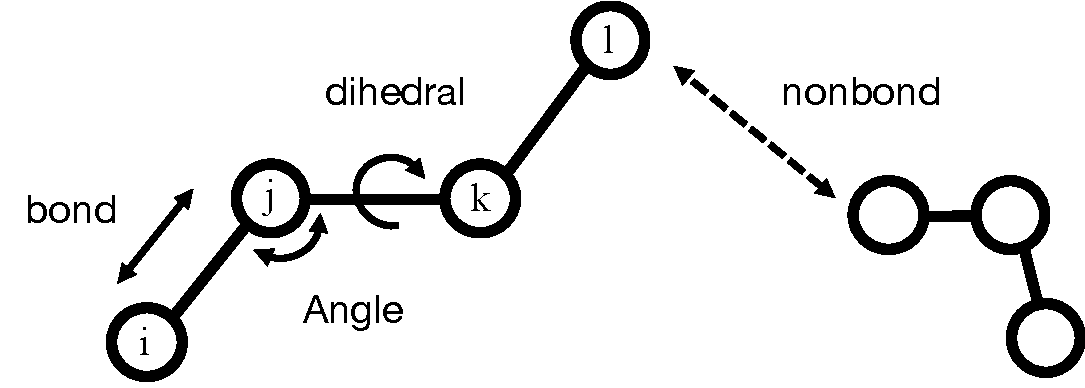
\includegraphics[width=0.5\hsize]{fig_biomol_model.pdf}
  \caption{生体分子の相互作用の模式図.}
  \label{Fig:BioModel}
 \end{center}
\end{figure}

\clearpage
\section{様々なポテンシャル関数: 力・ヴィリアルの表式}
この章では, 様々なポテンシャル関数を詳しく見ている.
また分子動力学シミュレーションの時間積分に必要な力や圧力計算に必要となるヴィリアルの
表式を解説する.
このノートでは位置ベクトルとして$\bm{r}_{ij} = \bm{r}_{j} - \bm{r}_{i}$の定義を使用する.

\subsection{結合長ポテンシャル: 調和振動子型}
\paragraph{結合長ポテンシャル}  \

共有結合をしている2原子間の相互作用は, 調和振動子で近似したポテンシャル関数
\begin{equation}
 U_{\mathrm{bond}}(r_{ij}) = k_{r} (r_{ij} - r_{\mathrm{eq}})^{2}
 \label{eq:BioModel2}
\end{equation}
を用いる. 
ここで, $k_{r}$はばね定数, $r_{ij}$は原子$i$と原子$j$の距離, $r_{\mathrm{eq}}$は平衡結合距離である.

\paragraph{結合長ポテンシャルの力} \

結合長による力は以下のように計算される:
\begin{alignat}{3}
    \bm{F}_{i}^{\mathrm{bond}}
 &= 
     -\frac{d U_{\mathrm{bond}}(r_{ij})}{d \bm{r}_{i}}
 &&= &
     2 k_{r} (r_{ij} - r_{\mathrm{eq}}) \frac{\bm{r}_{ij}}{r_{ij}}
 \label{eq:BioModel3}
 \\
 \bm{F}_{j}^{\mathrm{bond}}
 &=
   -\frac{d U_{\mathrm{bond}}(r_{ij})}{d \bm{r}_{j}}
 &&= -&
     2 k_{r} (r_{ij} - r_{\mathrm{eq}}) \frac{\bm{r}_{ij}}{r_{ij}}
 \label{eq:BioModel4}
\end{alignat}
ここで, 
\begin{equation}
 \bm{r}_{ij} = \bm{r}_{j} - \bm{r}_{i}
 \label{eq:BioModel4.5}
\end{equation}
とした.

\paragraph{結合長ポテンシャルのヴィリアル} \

ヴィリアルは
\begin{equation}
  -\left\langle
   \sum_{i=1}^{N} \bm{r}_{i}
   \cdot \frac{\partial U(\bm{r})}{\partial \bm{r}_{i}}
   \right\rangle
=
   \left\langle
   \sum_{i=1}^{N} \bm{r}_{i}
   \cdot \bm{F}_{i}
   \right\rangle
 \label{eq:BioModel5}
\end{equation}
で定義される. したがって, 結合長ポテンシャルに由来するヴィリアルは
\begin{align}
 \left\langle
   \sum_{i=1}^{N} \bm{r}_{i}
   \cdot \bm{F}_{i}
 \right\rangle
 &=
 \left\langle
   \sum_{\mathrm{bonds}}
   \left(
     \bm{r}_{i} \cdot \bm{F}_{i}^{\mathrm{bond}}
   + \bm{r}_{j} \cdot \bm{F}_{j}^{\mathrm{bond}}
 \right)
 \right\rangle
 \\
  &=
 \left\langle
   \sum_{\mathrm{bonds}}
   \left(
     \bm{r}_{ij} \cdot \bm{F}_{j}^{\mathrm{bond}}
 \right)
 \right\rangle
 \\
 &=
 \left\langle
      -\sum_{\mathrm{bonds}} 2 k_{r} (r_{ij} - r_{\mathrm{eq}}) r_{ij}
 \right\rangle
 \label{eq:BioModel6}
\end{align}
と計算される.

\clearpage

\subsection{結合長ポテンシャル: ガウス分布型}

\paragraph{ガウス分布型結合長ポテンシャル} \

共有結合をしている3つの原子$i,~j,~k$の結合角ポテンシャルを$i,~k$原子間の結合の相互作用として表すときにガウス分布型のポテンシャル関数

\begin{equation}
   U_{\mathrm{gauss}} (r_{ij})
   =
   \epsilon
   e^{-\frac{1}{2\sigma^{2}}(r_{ij} - r_{0})^{2}}
\end{equation}
を用いることがある. ここで, $r_{ij}$は原子$i$と原子$j$の距離, $r_{0}$は平行結合距離, $\epsilon$はポテンシャルの深さ, $\sigma$はポテンシャルの幅を表す.

\paragraph{ガウス分布型結合長ポテンシャルの力} \

ガウス分布型結合長ポテンシャルの力は以下のように計算される:

\begin{alignat}{3}
   \bm{F}_{i}^{\mathrm{gauss}}
   &=
   -&&
   \frac{\epsilon}{\sigma^{2}}
   (r_{ij} - r_{0})
   \cdot
   e^{-\frac{1}{2\sigma^{2}}(r_{ij} - r_{0})^{2}}
   \frac{\bm{r}_{ij}}{r_{ij}}
   \\
   \bm{F}_{j}^{\mathrm{gauss}}
   &=&&
   \frac{\epsilon}{\sigma^{2}}
   (r_{ij} - r_{0})
   \cdot
   e^{-\frac{1}{2\sigma^{2}}(r_{ij} - r_{0})^{2}}
   \frac{\bm{r}_{ij}}{r_{ij}}
\end{alignat}
ここで,
\begin{equation}
   \bm{r}_{ij} = \bm{r}_{j} - \bm{r}_{i}
\end{equation}
とした.


\paragraph{ガウス分布型結合長ポテンシャルのヴィリアル} \

ガウス分布型結合長ポテンシャルに由来するヴィリアルは
\begin{alignat}{3}
   \left\langle
      \bm{r}_{i} \cdot \bm{F}_{i}^{\mathrm{gauss}}
   \right\rangle
   =
   \left\langle
      \sum_{\mathrm{bonds}}
      \frac{\epsilon}{\sigma^{2}} r_{ij} (r_{ij} - r_{0})
      \cdot
      e^{-\frac{1}{2\sigma^{2}}(r_{ij} - r_{0})^{2}}
   \right\rangle
   \notag
\end{alignat}
と計算される.

\clearpage

\subsection{結合角ポテンシャル: 調和振動子型}
\paragraph{結合角ポテンシャル} \

共有結合をしている3つの原子間に関しては調和振動子で近似したポテンシャル関数
\begin{equation}
    U_{\mathrm{angle}}(\theta_{ijk})
  = k_{\theta} (\theta_{ijk} - \theta_{\mathrm{eq}})^{2}
 \label{eq:BioModel7}
\end{equation}
を用いる. ここで, $k_{\theta}$はばね定数, $\theta_{\mathrm{eq}}$は平衡結合角, 
$\theta_{ijk}$は結合角である. 
また, 
\begin{align}
  &\bm{r}_{ji}
 = \bm{r}_{i} - \bm{r}_{j}
 \label{eq:BioModel8}
 \\
  &\bm{r}_{jk}
 = \bm{r}_{k} - \bm{r}_{j}
 \label{eq:BioModel9}
 \\
  &\theta_{ijk}
 = \arccos \left(
                  \frac{\bm{r}_{ji} \cdot \bm{r}_{jk}}{r_{ji} r_{jk}}
           \right)
 \label{eq:BioModel10}
\end{align}
と定義した.

\paragraph{結合角ポテンシャルの力} \

 結合角による力は以下のように計算される:
\begin{alignat}{3}
     \bm{F}_{i}^{\mathrm{angle}}
 &= 
    -\frac{d U_{\mathrm{angle}}(\theta_{ijk})}{d \bm{r}_{i}}
 &&=
     2k_{\theta} (\theta_{ijk} - \theta_{\mathrm{eq}})
     \frac{1}{r_{ji} \sin \theta_{ijk}}
     \left(
            \frac{\bm{r}_{jk}}{r_{jk}} - \cos \theta_{ijk} \frac{\bm{r}_{ji}}{r_{ji}}
     \right)
 \label{eq:BioModel11}
 \\
     \bm{F}_{k}^{\mathrm{angle}}
 &= 
    -\frac{d U_{\mathrm{angle}}(\theta_{ijk})}{d \bm{r}_{k}}
 &&=
    2k_{\theta} (\theta_{ijk} - \theta_{\mathrm{eq}})
    \frac{1}{r_{jk} \sin \theta_{ijk}}
    \left(
           \frac{\bm{r}_{ji}}{r_{ji}} - \cos \theta_{ijk} \frac{\bm{r}_{jk}}{r_{jk}}
    \right)
 \label{eq:BioModel12}
 \\
     \bm{F}_{j}^{\mathrm{angle}}
 &= 
    -\frac{d U_{\mathrm{angle}}(\theta_{ijk})}{d \bm{r}_{j}}
 &&=
    -\bm{F}_{i}^{\mathrm{angle}} - \bm{F}_{k}^{\mathrm{angle}}
 \label{eq:BioModel13}
\end{alignat}

\paragraph{結合角ポテンシャルのヴィリアル} \

結合角ポテンシャルに由来するヴィリアルは, 
\begin{align}
    \bm{r}_{i} \cdot \bm{F}_{i}^{\mathrm{angle}}
   +\bm{r}_{j} \cdot \bm{F}_{j}^{\mathrm{angle}}
   +\bm{r}_{i} \cdot \bm{F}_{i}^{\mathrm{angle}}
 &=
    (\bm{r}_{i} - \bm{r}_{j}) \cdot \bm{F}_{i}^{\mathrm{angle}}
   +(\bm{r}_{k} - \bm{r}_{j}) \cdot \bm{F}_{k}^{\mathrm{angle}}
 \notag
 \\
 &=
    2k_{\theta} (\theta_{ijk} - \theta_{\mathrm{eq}}) \frac{1}{\sin \theta_{ijk}}
 \notag
 \\
 &~~~~ \times
    \left(
           \frac{\bm{r}_{ji} \cdot \bm{r}_{jk}}{r_{ji} r_{jk}} - \cos \theta_{ijk}
          +\frac{\bm{r}_{jk} \cdot \bm{r}_{ji}}{r_{jk} r_{ji}} - \cos \theta_{ijk}
    \right)
 \notag
 \\
 &=
    0
 \notag
\end{align}
であることからヴィリアルの値はゼロとなる. 

\clearpage

\subsection{角度に対するフィルター関数}

特定の角度周辺でのみポテンシャルを課すために, 次のようなフィルター関数をポテンシャル関数に乗じることがある:
\begin{align}
   f(K, \Delta \theta)
   =
   \begin{cases}
      1 &
      (\text{when}~\frac{-\pi}{2K} \le \Delta \theta \le \frac{\pi}{2K})\\
      1 - \cos^{2} (K \Delta \theta) &
      (\text{when}~\frac{-\pi}{K} < \Delta \theta < \frac{-\pi}{2K}~
       \text{or}~  \frac{\pi}{2K} < \Delta \theta < \frac{\pi}{K}) \\
      0 &
      (\text{when}~ \Delta \theta \le \frac{-\pi}{K}~
       \text{or}~ \Delta \theta \ge \frac{\pi}{K})
   \end{cases}
\end{align}
ここで, $K$はフィルター関数の幅を指定するパラメータ, $\Delta \theta = \theta_{ijk} - \theta_{0}$は目的の角度$\theta_{0}$からのずれである.
目的の角度周辺では1, 離れた領域では0, そしてそれらの領域の間を滑らかに繋いだ, 丘のような形をした関数となっている. なお, ここでは角度を
\begin{align}
   \bm{r}_{ji}
   &= \bm{r}_{i} - \bm{r}_{j}
   \\
   \bm{r}_{jk}
   &= \bm{r}_{k} - \bm{r}_{j}
   \notag \\
    \theta_{ijk}
   &= \arccos \left( \frac{\bm{r}_{ji} \cdot \bm{r}_{jk}}{r_{ji} r_{jk}} \right)
   \\
   \cos(\theta_{ijk})
   &= \frac{\bm{r}_{ji} \cdot \bm{r}_{jk}}{r_{ji} r_{jk}}
   = \frac{(\bm{r}_{i} - \bm{r}_{j}) \cdot (\bm{r}_{k} - \bm{r}_{j})}
         {\left\{(\bm{r}_{i} - \bm{r}_{j})\right\}^{\frac{1}{2}}
          \left\{(\bm{r}_{k} - \bm{r}_{j})\right\}^{\frac{1}{2}}}
\end{align}
と定義する.

\paragraph{フィルター関数に由来する力} \

フィルター関数に由来する力は
\begin{align}
   \bm{F}_{i}^{\mathrm{filter}}
   &=
   \frac{2K \sin (2K \Delta \theta)}{r_{ji} \sin\theta_{ijk}}
   \left(
            \frac{\bm{r}_{jk}}{r_{jk}}
          - \cos\theta_{ijk} \frac{\bm{r}_{ji}}{r_{ji}}
   \right)
   \\
   \bm{F}_{k}^{\mathrm{filter}}
   &=
   \frac{2K \sin (2K \Delta \theta)}{r_{jk} \sin\theta_{ijk}}
   \left(
           \frac{\bm{r}_{ji}}{r_{ji}}
         - \cos\theta_{ijk} \frac{\bm{r}_{jk}}{r_{jk}}
   \right)
   \\
   \bm{F}_{j}^{\mathrm{filter}}
   &=
   - \bm{F}_{i}^{\mathrm{filter}} - \bm{F}_{k}^{\mathrm{filter}}
\end{align}
のように計算することができる.



\clearpage
\subsection{二面角ポテンシャル: フーリエ級数型}
\paragraph{二面角ポテンシャル} \

共有結合した4原子が作る二面角に対するポテンシャルを,
\begin{equation}
    U_{\mathrm{dihedral}}(\phi_{ijkl})
  =
    \frac{V}{2} [1 + \cos(n\phi_{ijkl} - \gamma)]
 \label{eq:BioModel14}
\end{equation}
で表すことができる.
ここで, $V$はエネルギーバリア, $n$は周期, $\gamma$は位相である. 二面角$\phi_{ijkl}$は
\begin{alignat}{2}
 &\bm{r}_{ji} &&= \bm{r}_{i} - \bm{r}_{j}
 \label{eq:BioModel15}
 \\
 &\bm{r}_{kj} &&= \bm{r}_{j} - \bm{r}_{k}
 \label{eq:BioModel16}
 \\
 &\bm{r}_{lk} &&= \bm{r}_{k} - \bm{r}_{l}
 \label{eq:BioModel17}
 \\
 &\bm{n}_{j}  &&= \bm{r}_{ji} \times \bm{r}_{jk}
 \label{eq:BioModel18}
 \\
 &\bm{n}_{k}  &&= \bm{r}_{kj} \times \bm{r}_{kl}
 \label{eq:BioModel19}
 \\
 &\phi_{ijkl} &&=
 - \mathrm{sign}
   \left[
         \arccos \left( \frac{\bm{n}_{j} \cdot \bm{n}_{k}}{n_{j} n_{k}}\right)
         ,~
         \bm{r}_{kj} \cdot \bm{n}_{j} \times \bm{n}_{k}
   \right]
 \label{eq:BioModel20}
\end{alignat}
で定義される. 
ただし, $\mathrm{sign}[a,b]$は$(\mathrm{bの符号}) \times (\mathrm{aの絶対値})$と計算される. 

\paragraph{二面角ポテンシャルの力} \

二面角による力は以下のように計算される:
\begin{alignat}{3}
     \bm{F}_{i}^{\mathrm{dihedral}}
 &=
    -\frac{d U_{\mathrm{dihedral}}(\phi_{ijkl})}{d \bm{r}_{i}}
 &&=
     f_{0} (\bm{r}_{kj} \times \bm{f}_{\mathrm{kj}})
 \label{eq:BioModel21}
 \\
     \bm{F}_{j}^{\mathrm{dihedral}}
 &=
    -\frac{d U_{\mathrm{dihedral}}(\phi_{ijkl})}{d \bm{r}_{j}}
 &&=
     f_{0}
     \left( \bm{r}_{lk} \times \bm{f}_{jk}
           -\bm{r}_{kj} \times \bm{f}_{kj}
           -\bm{r}_{ji} \times \bm{f}_{kj}
     \right)
 \label{eq:BioModel22}
 \\
     \bm{F}_{k}^{\mathrm{dihedral}}
 &=
    -\frac{d U_{\mathrm{dihedral}}(\phi_{ijkl})}{d \bm{r}_{k}}
 &&=
    f_{0}
    \left( \bm{r}_{ji} \times \bm{f}_{kj}
          -\bm{r}_{lk} \times \bm{f}_{jk}
          -\bm{r}_{kj} \times \bm{f}_{jk}
    \right)
 \label{eq:BioModel23}
 \\
 \bm{F}_{l}^{\mathrm{dihedral}}
 &=
     -\frac{d U_{\mathrm{dihedral}}(\phi_{ijkl})}{d \bm{r}_{l}}
 &&=
     f_{0} ( \bm{r}_{kj} \times \bm{f}_{jk} )
 \label{eq:BioModel24}
\end{alignat}
ただし, 
\begin{align}
 f_{0}
 &=
    \frac{nV}{2} \frac{\sin(n \phi - \gamma)}{\sin \phi}
 \label{eq:BioModel25}
 \\
 \bm{f}_{kj}
 &=
    \frac{1}{n_{j}}
    \left(
           \frac{\bm{n}_{k}}{n_{k}} - \cos \phi \frac{\bm{n}_{j}}{n_{j}}
    \right)
 \label{eq:BioModel26}
 \\
 \bm{f}_{jk}
 &=
    \frac{1}{n_{k}}
    \left(
          \frac{\bm{n}_{j}}{n_{j}} - \cos \phi \frac{\bm{n}_{k}}{n_{k}}
    \right)
 \label{eq:BioModel27}
\end{align}
である. $\bm{f}_{\alpha}$($\alpha = 1, 2, 3, 4$)を
\begin{align}
 \bm{f}_{1} &= f_{0} ( \bm{r}_{kj} \times \bm{f}_{kj}) \\
 \bm{f}_{2} &= f_{0} ( \bm{r}_{lk} \times \bm{f}_{jk}) \\
 \bm{f}_{3} &= f_{0} ( \bm{r}_{ji} \times \bm{f}_{kj}) \\
 \bm{f}_{4} &= f_{0} ( \bm{r}_{kj} \times \bm{f}_{jk})
\end{align}
のように定義すると, 二面角による力は
\begin{align}
 \bm{F}_{i}^{\mathrm{dihedral}} &= \bm{f}_{1} \\
 \bm{F}_{j}^{\mathrm{dihedral}} &= \bm{f}_{2} - \bm{f}_{1} - \bm{f}_{3} \\
 \bm{F}_{k}^{\mathrm{dihedral}} &= \bm{f}_{3} - \bm{f}_{2} - \bm{f}_{4} \\
 \bm{F}_{l}^{\mathrm{dihedral}} &= \bm{f}_{4}
\end{align}
と書くことができる. 
 
\paragraph{二面角ポテンシャルのヴィリアル} \

ベクトル三重積の公式
\begin{align}
   \bm{A} \times (\bm{B} \times \bm{C})
 =
   (\bm{A} \cdot \bm{C}) \bm{B}
  -(\bm{A} \cdot \bm{B}) \bm{C}
\end{align}
を用いると, $\bm{f}_{kj}$と$\bm{f}_{jk}$は
\begin{align}
    \bm{f}_{kj}
 &=
    \frac{1}{n_{j}^{3} n_{k}}
    \left\{
            \bm{n}_{j} \times (\bm{n}_{k} \times \bm{n}_{j})
     \right\}
 \\
    \bm{f}_{jk}
 &=
    \frac{1}{n_{j} n_{k}^{3}}
    \left\{
            \bm{n}_{k} \times (\bm{n}_{j} \times \bm{n}_{k})
    \right\}
\end{align}
と書き直せる. さらに, 右辺に2つある$\bm{n}_{j}$あるいは$\bm{n}_k$に定義式(\ref{eq:BioModel18}), (\ref{eq:BioModel19})を代入して, 
ベクトル三重積の公式を繰り返し適用させると, 
\begin{align}
    \bm{n}_{j} \times (\bm{n}_{k} \times \bm{n}_{j})
 &=
   -(\bm{n}_{k} \cdot \bm{r}_{ji})
    \left\{
            (\bm{r}_{jk} \cdot \bm{r}_{jk})\bm{r}_{ji}
           -(\bm{r}_{jk} \cdot \bm{r}_{ji})\bm{r}_{jk}
    \right\}
 \\
    \bm{n}_{k} \times (\bm{n}_{j} \times \bm{n}_{k})
 &=
   -(\bm{n}_{j} \cdot \bm{r}_{kl})
    \left\{
            (\bm{r}_{kj} \cdot \bm{r}_{kl})\bm{r}_{kj}
           -(\bm{r}_{kj} \cdot \bm{r}_{kj})\bm{r}_{kl}
    \right\}
\end{align}
が得られ, 
\begin{align}
    \bm{f}_{1}
 &= 
    \frac{f_{0}}{n_{j}^{3}n_{k}}
    (\bm{n}_{k} \cdot \bm{r}_{ji})
    (\bm{r}_{jk} \cdot \bm{r}_{jk})
    (\bm{r}_{kj} \times \bm{r}_{ji})
 \\
    \bm{f}_{2}
 &= 
    \frac{-f_{0}}{n_{j}n_{k}^{3}}
    (\bm{n}_{j} \cdot \bm{r}_{kl})
    (\bm{r}_{kj} \cdot \bm{r}_{kl})
    (\bm{r}_{lk} \times \bm{r}_{kj})
 \\
    \bm{f}_{3}
 &= 
    \frac{-f_{0}}{n_{j}^{3}n_{k}}
    (\bm{n}_{k} \cdot \bm{r}_{ji})
    (\bm{r}_{jk} \cdot \bm{r}_{ji})
    (\bm{r}_{ji} \times \bm{r}_{jk})
 \\
    \bm{f}_{3}
 &= 
    \frac{f_{0}}{n_{j}n_{k}^{3}}
    (\bm{n}_{j} \cdot \bm{r}_{kl})
    (\bm{r}_{kj} \cdot \bm{r}_{kj})
    (\bm{r}_{kj} \times \bm{r}_{kl})
\end{align}
と計算される. これらを用いると,
\begin{align}
   \bm{r}_{i} \cdot \bm{F}_{i}^{\mathrm{dihedral}}
 + \bm{r}_{j} \cdot \bm{F}_{j}^{\mathrm{dihedral}}
 + \bm{r}_{k} \cdot \bm{F}_{k}^{\mathrm{dihedral}}
 + \bm{r}_{l} \cdot \bm{F}_{l}^{\mathrm{dihedral}}
 = 0
\end{align}
となることが確認できるため, 二面角ポテンシャルに由来するヴィリアルはゼロとなる. 

\clearpage

\subsection{二面角ポテンシャル: ガウス分布型}

\paragraph{ガウス分布型二面角ポテンシャル} \

共有結合をしている3つの原子$i,~j,~k,~l$の二面角ポテンシャルをガウス分布型のポテンシャル関数
\begin{equation}
   U_{\mathrm{gauss}} (\phi_{ijkl})
   =
   \epsilon
   e^{-\frac{1}{2\sigma^{2}}(\phi_{ijkl} - \phi_{0})^{2}}
\end{equation}
を用いて表すことがある. ここで, $r_{ij}$は原子$i$と原子$j$の距離, $r_{0}$は平行結合距離, $\epsilon$はポテンシャルの深さ, $\sigma$はポテンシャルの幅を表す. ここで二面角は
\begin{alignat}{1}
   \bm{r}_{ji} &= \bm{r}_{i} - \bm{r}_{j}
   \notag \\
   \bm{r}_{kj} &= \bm{r}_{j} - \bm{r}_{k}
   \notag \\
   \bm{r}_{lk} &= \bm{r}_{k} - \bm{r}_{l}
   \notag \\
   \bm{n}_{j}  &= \bm{r}_{ji} \times \bm{r}_{jk}
   \notag \\
   \bm{n}_{k}  &= \bm{r}_{kj} \times \bm{r}_{kl}
   \notag
   \\
   \phi_{ijkl} &=
   - \mathrm{sign}
     \left[
           \arccos \left( \frac{\bm{n}_{j} \cdot \bm{n}_{k}}{n_{j} n_{k}}\right),
           \bm{r}_{kj} \cdot \bm{n}_{j} \times \bm{n}_{k}
     \right]
   \notag
\end{alignat}
と定義する.

\paragraph{ガウス分布型二面角ポテンシャルの力} \

ガウス分布型二面角ポテンシャルの力は係数を除いて, フーリエ級数型ポテンシャルと同じように計算することができる.
すなわち, 
\begin{align}
   f_{0}
   &\equiv
   \frac{\epsilon(\phi_{ijkl} - \phi_{0})}{\sigma^{2} \sin \phi_{ijkl}}
   e^{-\frac{1}{2\sigma^{2}}(\phi_{ijkl} - \phi_{0})^{2}}
   \\
   \bm{f}_{kj}
   &\equiv
   \left\{
      \frac{1}{n_{j}}
      \left(
             \frac{\bm{n}_{k}}{n_{k}} - \cos\phi \frac{\bm{n}_{j}}{n_{j}}
      \right)
   \right\}
   \\
   \bm{f}_{jk}
   &\equiv
   \left\{
      \frac{1}{n_{k}}
      \left(
             \frac{\bm{n}_{j}}{n_{j}} - \cos\phi \frac{\bm{n}_{k}}{n_{k}}
      \right)
   \right\}
\end{align}
と置いた時に, 各粒子に加わる力は
\begin{alignat}{5}
   \bm{F}_{i}
   &=
   &&
   f_{0} (\bm{r}_{kj} \times \bm{f}_{kj})
   \\
   \bm{F}_{j}
   &=
   &&
   f_{0} (\bm{r}_{lk} \times \bm{f}_{jk} - \bm{r}_{ki} \times \bm{f}_{kj})
   &=
   f_{0}
   ( \bm{r}_{lk} \times \bm{f}_{jk}
   - \bm{r}_{kj} \times \bm{f}_{kj}
   - \bm{r}_{ji} \times \bm{f}_{kj} )
   \\
   \bm{F}_{k}
   &=&&
   f_{0} (\bm{r}_{ji} \times \bm{f}_{kj} - \bm{r}_{lj} \times \bm{f}_{jk})
   &=
   f_{0}
   ( \bm{r}_{ji} \times \bm{f}_{kj}
   - \bm{r}_{lk} \times \bm{f}_{jk}
   - \bm{r}_{kj} \times \bm{f}_{jk})
   \\
   \bm{F}_{l}
   &=&&
   f_{0} (\bm{r}_{kj} \times \bm{f}_{jk})
\end{alignat}
と計算できる.


\paragraph{ガウス分布型二面角ポテンシャルのヴィリアル} \

ガウス分布型二面角ポテンシャルの力の表式が, 係数$f_{0}$を除いてフーリエ級数型の二面角ポテンシャルと同じであることに注目すると, フーリエ級数型の二面角ポテンシャルの時と同様の計算によって
\begin{align}
   \bm{r}_{i} \cdot \bm{F}_{i}^{\mathrm{dihedral}}
 + \bm{r}_{j} \cdot \bm{F}_{j}^{\mathrm{dihedral}}
 + \bm{r}_{k} \cdot \bm{F}_{k}^{\mathrm{dihedral}}
 + \bm{r}_{l} \cdot \bm{F}_{l}^{\mathrm{dihedral}}
 = 0
\end{align}
となることが確認できる. すなわち, ガウス分布型二面角ポテンシャルのヴィリアルはゼロとなる.

\clearpage
\subsection{ファンデル・ワールス相互作用: 12-6型}
\paragraph{ファンデル・ワールス相互作用} \

ファンデル・ワールス相互作用によるポテンシャルは, レナード・ジョーンズポテンシャル用いて
\begin{equation}
    U_{\mathrm{LJ}}(r_{ij})
 =
   4\epsilon_{ij}
   \left\{
           \left(\frac{\sigma_{ij}}{r_{ij}}\right)^{12}
          -\left(\frac{\sigma_{ij}}{r_{ij}}\right)^{6}
   \right\}
 \label{eq:BioModel29}
\end{equation}
と与えられる.
ここで, $\epsilon_{ij}$はポテンシャルの深さ, $\sigma_{ij}$は粒子間の最小相互作用距離, 
$r_{ij}$は粒子間の距離を表している. 
第1項目は電子雲の重なりに起因する反発項, 第2項目は分散力に起因する引力項である. 
$\epsilon_{ij}$と$\sigma_{ij}$はローレンツ・ベルテロー則を用いて
各原子についてのポテンシャルの深さ$\epsilon_{i}$と粒子の直径$\sigma_{i}$から
\begin{align}
 \epsilon_{ij} &= \sqrt{\epsilon_{i} \epsilon_{j}}
 \\
 \sigma  _{ij} &= \frac{\sigma_{i} + \sigma_{j}}{2}
 \label{eq:BioModel30}
\end{align}
で与えられることが多い.
LJ相互作用の計算は$\mathcal{O}(N^2)$となり計算コストがかかる. 
しかし, 収束の速い関数であるため通常はカットオフを設定し, カットオフ半径内に存在する粒子対のみ計算することで
計算コストを抑えることができる. 
カットオフ半径$r_{c}$は系のボックスサイズの半分以下の大きさの値に設定する. 

\paragraph{ファンデル・ワールス相互作用の力} \

レナード・ジョーンズ相互作用による力は以下のように計算される:
\begin{alignat}{3}
    \bm{F}_{i}^{\mathrm{LJ}}
 &=
   -\frac{d U_{\mathrm{LJ}}(r_{ij})}{d \bm{r}_{i}}
  =
   -&&
   24 \epsilon_{ij}
   \left\{
           2\left( \frac{\sigma_{ij}}{r_{ij}} \right)^{12}
          - \left( \frac{\sigma_{ij}}{r_{ij}} \right)^{6}
   \right\}
   \frac{\bm{r}_{ij}}{r_{ij}^{2}}
 \label{eq:BioModel31}
 \\
    \bm{F}_{j}^{\mathrm{LJ}}
 &=
   -\frac{d U_{\mathrm{LJ}}(r_{ij})}{d \bm{r}_{j}}
 =
   &&
   24 \epsilon_{ij}
   \left\{
           2\left( \frac{\sigma_{ij}}{r_{ij}} \right)^{12}
          - \left( \frac{\sigma_{ij}}{r_{ij}} \right)^{6}
   \right\}
   \frac{\bm{r}_{ij}}{r_{ij}^{2}}
 \label{eq:BioModel32}
\end{alignat}

\paragraph{ファンデル・ワールス相互作用のヴィリアル} \

ファンデル・ワールス相互作用に由来するヴィリアルは, 
\begin{align}
 &\left\langle
  \sum_{i=1}^{N} \sum_{j > i}^{N}
  24 \epsilon_{ij}
  \left\{
        2 \left( \frac{\sigma_{ij}}{r_{ij}} \right)^{12}
        - \left( \frac{\sigma_{ij}}{r_{ij}} \right)^{6}
  \right\}
 \right\rangle
 \\
 =
  &\left\langle
   \sum_{\mathrm{nonbonds}}
   24 \epsilon_{ij}
   \left\{
           2\left( \frac{\sigma_{ij}}{r_{ij}} \right)^{12}
          - \left( \frac{\sigma_{ij}}{r_{ij}} \right)^{6}
   \right\}
   \right\rangle
 \label{eq:BioModel33}
\end{align}
で計算される. 

\clearpage

\subsection{モースポテンシャル}
\paragraph{モースポテンシャル} \

モースポテンシャルは2原子の結合・解離を記述するときに使用されるポテンシャルである.
具体的なポテンシャル関数は,

\begin{equation}
   U_{\mathrm{morse}} (r_{ij})
   =
   \epsilon
   \left\{
      1 - e^{-\alpha(r_{ij} - r_{0})}
   \right\}^{2}
\end{equation}
とかける. ここで, $r_{ij}$は2原子間の距離, $\epsilon$はポテンシャルの深さ, $\alpha$はポテンシャルの幅, $r_{i}$は2原子の平衡結合距離を表す.

\paragraph{モースポテンシャルによる力} \

モースポテンシャルによって原子がうける力は以下のように計算される.
\begin{alignat}{3}
   \bm{F}_{i}^{\mathrm{morse}}
   =
   -
   \frac{d U_{\mathrm{morse}}(r_{ij})}{d \bm{r}_{i}}
   &=&&
   2\epsilon \alpha
   \left\{
      e^{-\alpha(r_{ij} - r_{0})}
      -
      e^{-2\alpha(r_{ij} - r_{0})}
   \right\}
   \frac{\bm{r}_{ij}}{r_{ij}}
   \\
   \bm{F}_{j}^{\mathrm{morse}}
   =
   -
   \frac{d U_{\mathrm{morse}}(r_{ij})}{d \bm{r}_{j}}
   &=
   -&&
   2\epsilon \alpha
   \left\{
      e^{-\alpha(r_{ij} - r_{0})}
      -
      e^{-2\alpha(r_{ij} - r_{0})}
   \right\}
   \frac{\bm{r}_{ij}}{r_{ij}}
\end{alignat}
ただし,
\begin{align}
   \bm{r}_{ij} = \bm{r}_{j} - \bm{r}_{i}
\end{align}
と定義した.

\paragraph{モースポテンシャルに由来するヴィリアル} \

モースポテンシャル相互作用に由来するヴィリアルは, 
\begin{align}
   \left\langle
        \sum_{i=1}^{N} \bm{r}_{i} \cdot \bm{F}_{i}^{\mathrm{morse}}
   \right\rangle
 =
   \left\langle
        \sum_{\mathrm{nonbonds}}
        -2\epsilon \alpha r_{ij}
        \left\{
           e^{-\alpha(r_{ij} - r_{0})}
           -
           e^{-2\alpha(r_{ij} - r_{0})}
        \right\}
   \right\rangle
\end{align}
と計算できる.

\clearpage

\subsection{静電相互作用}
\paragraph{静電ポテンシャル} \

電磁気でよく知られるように静電ポテンシャルは

\begin{equation}
U_{\mathrm{elec}}(r_{ij}) = \frac{q_{i}q_{j}}{4 \pi \epsilon_{0}}
                            \frac{1}{r_{ij}}
\end{equation}
とかける.
$q_{i}$と$q_{j}$はそれぞれ原子$i$と原子$j$の電荷, $\epsilon_{0}$は真空中の誘電率, 
$r_{ij}$は原子$i$と原子$j$の距離である.

静電相互作用はレナードジョーンズ相互作用と比較して, 減衰が遅いポテンシャル関数である.
そのため計算コストを減少するためのカットオフをしてしまうと誤差を生み出す原因となる.
このような問題を回避するための方法として, Ewald法やParticle Mesh Ewald法,
多極子展開法など様々な取扱方法がこれまでに提案されてきている\cite{2014Cisneros}.

\paragraph{静電ポテンシャルによる力} \

静電相互作用による力は以下のように計算される.
\begin{alignat}{3}
   \bm{F}_{i}^{\mathrm{elec}}
 &=
   -\frac{d U_{\mathrm{elec}}(r_{ij})}{d \bm{r}_{i}}
&&=&
   -\frac{q_{i}q_{j}}{4 \pi \epsilon_{0} r_{ij}^{2}}
    \frac{\bm{r}_{ij}}{r_{ij}}
 \\
    \bm{F}_{j}^{\mathrm{elec}}
 &=
   -\frac{d U_{\mathrm{elec}}(r_{ij})}{d \bm{r}_{j}}
&&=&
    \frac{q_{i}q_{j}}{4 \pi \epsilon_{0} r_{ij}^{2}}
    \frac{\bm{r}_{ij}}{r_{ij}}
 \\
\end{alignat}

\paragraph{静電ポテンシャルによるヴィリアル} \

静電相互作用に由来するヴィリアルは,
\begin{align}
  \left\langle
  \sum_{i=1}^{N} \sum_{j > i}^{N}
  \frac{q_{i}q_{j}}{4 \pi \epsilon_{0}}
  \frac{1}{r_{ij}}
  \right\rangle
 =
  \left\langle
  \sum_{\mathrm{nonbonds}}
  \frac{q_{i}q_{j}}{4 \pi \epsilon_{0}}
  \frac{1}{r_{ij}}
  \right\rangle
\end{align}
となる.

\clearpage
\section{計算ノート: 微分・力・ヴィリアルの導出}
\subsection{力の計算の基本的な手順}
粒子$\alpha$に加わる力は, ポテンシャルを座標ベクトル$\bm{r}_{\alpha}$に関して微分すれば良い. すなわち

\begin{align}
   \bm{F}_{\alpha}
   =
   -
   \frac{d U}{d \bm{r}_{\alpha}}
\end{align}
と計算できる.
代表的なポテンシャル関数として(1)調和振動子, (2)ガウス関数, (3) フーリエ級数 ($\cos$関数, $\sin$関数), (4) レナード・ジョーンズポテンシャル, (5) モースポテンシャル, (6)静電相互作用がある.
さらに, 多くの場合でポテンシャル関数は内部座標を用いて表されることが多い.
例えば, 2体相互作用であれば, 2点間の距離$r_{ij}$, 3体相互作用であれば, 3点間の角度$\theta_{ijk}$, 4体相互作用であれば4点間の二面角$\phi_{ijkl}$の関数で表されることが多い.

微分の連鎖率を用いると, 力の計算は(i)ポテンシャルの変数に関する微分, (ii)ポテンシャルの変数の座標ベクトル微分の積で書くことができる. すなわち
\begin{align}
   \bm{F}_{\alpha}
   =
   -
   \frac{d U}{d \lambda}
   \frac{d \lambda}{d \bm{r}_{\alpha}}
\end{align}
となる. 第1項目はポテンシャル関数形ごとに計算される項である. 第2項目は内部座標に依存する項で, 力の向きに関係してくる.


\subsection{2点間の距離$r_{ij}$を粒子の位置ベクトル$\bm{r}_{\alpha}$で微分する}
\subsubsection{ベクトルの定義}
質点の位置$\bm{r}_{i}$から$\bm{r}_{j}$に向かうベクトルを
\begin{align}
   \bm{r}_{ij}
&= \bm{r}_{j} - \bm{r}_{i}
\end{align}
と定義する. 2点間の距離は
\begin{align}
   r_{ij} = \left(\bm{r}_{ij} \cdot \bm{r}_{ij} \right)^{\frac{1}{2}}
\end{align}
と計算される.
\subsubsection{座標ベクトル微分の計算}
\begin{align}
\frac{d r_{ij}}{d \bm{r}_{i}}
&=
\left[
   \frac{d}{d \bm{r}_{i}}
   \left\{ (\bm{r}_{j} - \bm{r}_{i} )^{2} \right\}^{\frac{1}{2}}
\right]
=
\frac{1}{2}
\frac{ -2 (\bm{r}_{j} - \bm{r}_{i}) }
     { \left\{ ( \bm{r}_{j} - \bm{r}_{i} )^{2} \right\}^{\frac{1}{2}} }
=
-
\frac{\bm{r}_{ij}}{r_{ij}}
\label{Eq:dr_ij-dr_i}
\\
\frac{d r_{ij}}{d \bm{r}_{j}}
&=
\left[
   \frac{d}{d \bm{r}_{j}}
   \left\{ (\bm{r}_{j} - \bm{r}_{i} )^{2} \right\}^{\frac{1}{2}}
\right]
=
\frac{1}{2}
\frac{ 2 (\bm{r}_{j} - \bm{r}_{i}) }
     { \left\{ ( \bm{r}_{j} - \bm{r}_{i} )^{2} \right\}^{\frac{1}{2}} }
=
\frac{\bm{r}_{ij}}{r_{ij}}
\label{Eq:dr_ij-dr_j}
\end{align}

\subsection{3点間の角度$\theta_{ijk}$を粒子の位置ベクトル$\bm{r}_{\alpha}$で微分する}
\subsubsection{ベクトルと角度の定義}
3点間の角度$\theta_{ijk}$を
\begin{align}
   \bm{r}_{ji}
&= \bm{r}_{i} - \bm{r}_{j}
\\
   \bm{r}_{jk}
&= \bm{r}_{k} - \bm{r}_{j}
\\
   \theta_{ijk}
&= \arccos \left( \frac{\bm{r}_{ji} \cdot \bm{r}_{jk}}{r_{ji} r_{jk}} \right)
\\
   \cos(\theta_{ijk})
&= \frac{\bm{r}_{ji} \cdot \bm{r}_{jk}}{r_{ji} r_{jk}}
 = \frac{(\bm{r}_{i} - \bm{r}_{j}) \cdot (\bm{r}_{k} - \bm{r}_{j})}
        {\left\{(\bm{r}_{i} - \bm{r}_{j})\right\}^{\frac{1}{2}}
         \left\{(\bm{r}_{k} - \bm{r}_{j})\right\}^{\frac{1}{2}}}
\end{align}
と定義する.

\subsubsection{座標ベクトル微分の計算}
3点間の角度$\theta_{ijk}$を粒子の位置ベクトル$\bm{r}_{\alpha}$で微分すると
\begin{align}
    \frac{d \theta_{ijk}}{d \bm{r}_{\alpha}}
 &=
    \frac{d}{d \bm{r}_{\alpha}}
    \arccos \left( \frac{\bm{r}_{ji} \cdot \bm{r}_{jk}}{r_{ji} r_{jk}} \right)
 \notag \\
 &=
   -\frac{1}
         {\sqrt{1- \left(\frac{\bm{r}_{ji} \cdot \bm{r}_{jk}}{r_{ji} r_{jk}}\right)^{2}}}
    \left\{
            \frac{d}{d \bm{r}_{\alpha}}
            \left(\frac{\bm{r}_{ji} \cdot \bm{r}_{jk}}{r_{ji} r_{jk}}\right)
    \right\}
 \notag \\
 &=
   -\frac{1}{\sin\theta_{ijk}}
    \left\{
            \frac{d}{d \bm{r}_{\alpha}}
            \left(\frac{\bm{r}_{ji} \cdot \bm{r}_{jk}}{r_{ji} r_{jk}}\right)
    \right\}
  \notag
\end{align}
を得る. 第2式から第3式において, $\arccos(x)$の微分公式
\begin{equation}
\frac{d}{dx}\arccos(x) = - \frac{1}{\sqrt{1-x^2}}
\notag
\end{equation}
を用いた. 続いて
\begin{equation}
 \frac{d}{d \bm{r}_{\alpha}}
 \left(\frac{\bm{r}_{ji} \cdot \bm{r}_{jk}}{r_{ji} r_{jk}}\right)
 \notag
\end{equation}
を各粒子$i$,$j$,$k$について計算していく.

\paragraph{$\alpha = i$のとき}
\begin{align}
    \frac{d}{d \bm{r}_{i}}
    \left(\frac{\bm{r}_{ji} \cdot \bm{r}_{jk}}{r_{ji} r_{jk}}\right)
 &=
    \frac{d}{d \bm{r}_{i}}
    \left[\frac{(\bm{r}_{i} - \bm{r}_{j}) \cdot (\bm{r}_{k} - \bm{r}_{j})}
               {\left\{ (\bm{r}_{i} - \bm{r}_{j})^{2} \right\}^{\frac{1}{2}}
                \left\{ (\bm{r}_{k} - \bm{r}_{j})^{2} \right\}^{\frac{1}{2}}}
    \right]
 \notag \\
 &=
    \frac{d}{d \bm{r}_{i}}
    \left[(\bm{r}_{i} - \bm{r}_{j}) \cdot (\bm{r}_{k} - \bm{r}_{j})
           \left\{ (\bm{r}_{i} - \bm{r}_{j})^{2} \right\}^{-\frac{1}{2}}
           \left\{ (\bm{r}_{k} - \bm{r}_{j})^{2} \right\}^{-\frac{1}{2}}
    \right]
 \notag \\
 &=
     \frac{(\bm{r}_{k} - \bm{r}_{j})}{r_{ji} r_{jk}}
   - \frac{1}{2}
     \frac{2(\bm{r}_{i} - \bm{r}_{j})
           \{(\bm{r}_{i} - \bm{r}_{j}) \cdot (\bm{r}_{k} - \bm{r}_{j})\}}
          {\left\{ (\bm{r}_{i} - \bm{r}_{j})^{2} \right\}^{\frac{3}{2}}
           \left\{ (\bm{r}_{k} - \bm{r}_{j})^{2} \right\}^{\frac{1}{2}}}
 \notag \\
 &=
     \frac{\bm{r}_{jk}}{r_{ji} r_{jk}}
   - \frac{(\bm{r}_{ji} \cdot \bm{r}_{jk}) \bm{r}_{ji}}{r_{ji}^{3} r_{jk}}
 \notag \\
 &=
     \frac{1}{r_{ji}}
     \left\{
              \frac{\bm{r}_{jk}}{r_{jk}}
            - \cos\theta_{ijk} \frac{\bm{r}_{ji}}{r_{ji}}
     \right\}
\notag
\end{align}
と計算できる.

\paragraph{$\alpha = k$のときの$\bm{F}^{\mathrm{angle}}$の導出} \

$\alpha=i$と同様の計算により, 
\begin{align}
   \frac{d}{d \bm{r}_{k}}
   \left(\frac{\bm{r}_{ji} \cdot \bm{r}_{jk}}{r_{ji} r_{jk}}\right)
&=
   \frac{1}{r_{jk}}
   \left(
           \frac{\bm{r}_{ji}}{r_{ji}}
         - \cos\theta_{ijk} \frac{\bm{r}_{jk}}{r_{jk}}
   \right)
\notag
\end{align}
と計算される. \\

\paragraph{$\alpha = j$のときの$\bm{F}^{\mathrm{angle}}$の導出} \
\begin{align}
    \frac{d}{d \bm{r}_{j}}
    \left(\frac{\bm{r}_{ji} \cdot \bm{r}_{jk}}{r_{ji} r_{jk}}\right)
 =&
    \frac{d}{d \bm{r}_{j}}
    \left[\frac{(\bm{r}_{i} - \bm{r}_{j}) \cdot (\bm{r}_{k} - \bm{r}_{j})}
               {\left\{ (\bm{r}_{i} - \bm{r}_{j})^{2} \right\}^{\frac{1}{2}}
                \left\{ (\bm{r}_{k} - \bm{r}_{j})^{2} \right\}^{\frac{1}{2}}}
    \right]
 \notag \\
 =&
    \frac{d}{d \bm{r}_{j}}
    \left[(\bm{r}_{i} - \bm{r}_{j}) \cdot (\bm{r}_{k} - \bm{r}_{j})
           \left\{ (\bm{r}_{i} - \bm{r}_{j})^{2} \right\}^{-\frac{1}{2}}
           \left\{ (\bm{r}_{k} - \bm{r}_{j})^{2} \right\}^{-\frac{1}{2}}
    \right]
 \notag \\
 =&
   - \frac{(\bm{r}_{k} - \bm{r}_{j})}{r_{ji} r_{jk}}
   - \frac{1}{2}
     \frac{-2(\bm{r}_{i} - \bm{r}_{j})
            \{(\bm{r}_{i} - \bm{r}_{j}) \cdot (\bm{r}_{k} - \bm{r}_{j})\}}
          {\left\{ (\bm{r}_{i} - \bm{r}_{j})^{2} \right\}^{\frac{3}{2}}
           \left\{ (\bm{r}_{k} - \bm{r}_{j})^{2} \right\}^{\frac{1}{2}}}
 \notag \\
 & - \frac{(\bm{r}_{k} - \bm{r}_{j})}{r_{ji} r_{jk}}
   - \frac{1}{2}
     \frac{-2(\bm{r}_{k} - \bm{r}_{j})
            \{(\bm{r}_{i} - \bm{r}_{j}) \cdot (\bm{r}_{k} - \bm{r}_{j})\}}
          {\left\{ (\bm{r}_{i} - \bm{r}_{j})^{2} \right\}^{\frac{1}{2}}
           \left\{ (\bm{r}_{k} - \bm{r}_{j})^{2} \right\}^{\frac{3}{2}}}
 \notag \\
 =& - \left\{
               \frac{\bm{r}_{jk}}{r_{ji} r_{jk}}
             - \frac{(\bm{r}_{ji} \cdot \bm{r}_{jk}) \bm{r}_{ji}}{r_{ji}^{3} r_{jk}}
      \right\}
    - \left\{
               \frac{\bm{r}_{ji}}{r_{ji} r_{ji}}
             - \frac{(\bm{r}_{ji} \cdot \bm{r}_{jk}) \bm{r}_{jk}}{r_{ji} r_{jk}^{3}}
      \right\}
 \notag \\
 =&
   - \frac{1}{r_{ji}}
     \left\{
              \frac{\bm{r}_{jk}}{r_{jk}}
            - \cos\theta_{ijk} \frac{\bm{r}_{ji}}{r_{ji}}
     \right\}
   - \frac{1}{r_{jk}}
     \left\{
              \frac{\bm{r}_{ji}}{r_{ji}}
            - \cos\theta_{ijk} \frac{\bm{r}_{jk}}{r_{jk}}
     \right\}
\notag
\end{align}
と計算できる.

\paragraph{まとめ}
以上をまとめると, 3点間の角度$\theta_{ijk}$の粒子の位置ベクトル$\bm{r}_{\alpha}$微分は,

\begin{alignat}{3}
   \frac{d \theta_{ijk}}{d \bm{r}_{i}}
   &=
   -&&
   \frac{1}{r_{ji} \sin\theta_{ijk}}
   \left(
            \frac{\bm{r}_{jk}}{r_{jk}}
          - \cos\theta_{ijk} \frac{\bm{r}_{ji}}{r_{ji}}
   \right)
   \label{Eq:dtheta_dri}
   \\
   \frac{d \theta_{ijk}}{d \bm{r}_{j}}
   &=&&
   \frac{1}{r_{ji} \sin\theta_{ijk}}
   \left(
            \frac{\bm{r}_{jk}}{r_{jk}}
          - \cos\theta_{ijk} \frac{\bm{r}_{ji}}{r_{ji}}
   \right)
   +
   \frac{1}{r_{jk} \sin\theta_{ijk}}
   \left(
            \frac{\bm{r}_{ji}}{r_{ji}}
          - \cos\theta_{ijk} \frac{\bm{r}_{jk}}{r_{jk}}
   \right)
   \label{Eq:dtheta_drj}
   \\
   \frac{d \theta_{ijk}}{d \bm{r}_{k}}
   &=
   -&&
   \frac{1}{r_{jk} \sin\theta_{ijk}}
   \left(
           \frac{\bm{r}_{ji}}{r_{ji}}
         - \cos\theta_{ijk} \frac{\bm{r}_{jk}}{r_{jk}}
   \right)
   \label{Eq:dtheta_drk}
\end{alignat}
と計算される. 

\subsection{二面角$\phi_{ijkl}$を粒子の位置ベクトル$\bm{r}_{\alpha}$で微分する}
\subsubsection{ベクトルと二面角の定義}
二面角$\phi_{ijkl}$を
\begin{alignat}{1}
   \bm{r}_{ji} &= \bm{r}_{i} - \bm{r}_{j}
   \notag \\
   \bm{r}_{kj} &= \bm{r}_{j} - \bm{r}_{k}
   \notag \\
   \bm{r}_{lk} &= \bm{r}_{k} - \bm{r}_{l}
   \notag \\
   \bm{n}_{j}  &= \bm{r}_{ji} \times \bm{r}_{jk}
   \notag \\
   \bm{n}_{k}  &= \bm{r}_{kj} \times \bm{r}_{kl}
   \notag
   \\
   \phi_{ijkl} &=
   - \mathrm{sign}
     \left[
           \arccos \left( \frac{\bm{n}_{j} \cdot \bm{n}_{k}}{n_{j} n_{k}}\right),
           \bm{r}_{kj} \cdot \bm{n}_{j} \times \bm{n}_{k}
     \right]
   \notag
\end{alignat}
と定義する.

\subsubsection{座標ベクトル微分の計算}

$\cos$の微分 
\begin{align}
 d \cos\phi &= -\sin\phi d\phi
 \notag
\end{align}
から, 二面角$\phi_{ijkl}$の位置座標ベクトル微分は
\begin{align}
     \frac{d \phi_{ijkl}}{d \bm{r}_{\alpha}}
 = - \frac{1}{\sin\phi_{ijkl}} \frac{d \cos\phi_{ijkl}}{d \bm{r}_{\alpha}}
 = - \frac{1}{\sin\phi_{ijkl}} \frac{d} {d \bm{r}_{\alpha}}
     \left(
           \frac{\bm{n}_{j} \cdot \bm{n}_{k}} {n_{j} n_{k}}
     \right)
 \notag
\end{align}
と計算できる. よって, $\alpha = i, j, k, l$に対する二面角$\phi_{ijkl}$の位置座標ベクトル微分は
\begin{align}
    \frac{d}{d \bm{r}_{\alpha}}
    \left( \frac{\bm{n}_{j} \cdot \bm{n}_{k}} {n_{j} n_{k}} \right)
 =
    \frac{1}{n_{j}n_{k}}
    \left\{
           \frac{d}{d \bm{r}_{\alpha}} (\bm{n}_{j} \cdot \bm{n}_{k})
    \right\}
  +
    \frac{\bm{n}_{k} \cdot \bm{n}_{k}}{n_{k}}
    \left\{
           \frac{d}{d \bm{r}_{\alpha}} \frac{1}{n_{j}}
    \right\}
  +
    \frac{\bm{n}_{j} \cdot \bm{n}_{k}}{n_{j}}
    \left\{
           \frac{d}{d \bm{r}_{\alpha}} \frac{1}{n_{k}}
    \right\}
 \notag
\end{align}
を求めることに帰着する. ここで, 
\begin{alignat}{3}
 \bm{n}_{j} &=  \bm{r}_{ji} \times \bm{r}_{jk}
 \notag \\
                &=  \bm{r}_{i} \times \bm{r}_{k}
                  - \bm{r}_{i} \times \bm{r}_{j}
                  - \bm{r}_{j} \times \bm{r}_{k}
 \notag \\
 \bm{n}_{k} &=  \bm{r}_{kj} \times \bm{r}_{kl}
 \notag \\
                &=  \bm{r}_{j} \times \bm{r}_{l}
                  - \bm{r}_{j} \times \bm{r}_{k}
                  - \bm{r}_{k} \times \bm{r}_{l}
 \notag \\
 \frac{1}{n_{j}} &= \left\{(  \bm{r}_{i} \times \bm{r}_{k}
                            - \bm{r}_{i} \times \bm{r}_{j}
                            - \bm{r}_{j} \times \bm{r}_{k} )^{2}
                    \right\}^{-\frac{1}{2}}
 \notag \\
 \frac{1}{n_{k}} &= \left\{(  \bm{r}_{j} \times \bm{r}_{l}
                            - \bm{r}_{j} \times \bm{r}_{k}
                            - \bm{r}_{k} \times \bm{r}_{l} )^{2}
                    \right\}^{-\frac{1}{2}}
 \notag
\end{alignat}
と書き下せる. 
\\

\paragraph{いくつかの便利な公式} \
今後の計算の便利のためにベクトルの微分に関する公式を導出する. ベクトル$\bm{a}, \bm{b}, \bm{c}$を考える. 
\begin{align}
 \bm{a}= \left(
              \begin{array}{c}
               a_{x} \\
               a_{y} \\
               a_{z} 
              \end{array}
              \right)
 ,~~~
 \bm{b}= \left(
              \begin{array}{c}
               b_{x} \\
               b_{y} \\
               b_{z} 
              \end{array}
              \right)
 ,~~~
 \bm{c}= \left(
              \begin{array}{c}
               c_{x} \\
               c_{y} \\
               c_{z} 
              \end{array}
              \right)
\notag
\end{align}
ベクトルの内積は
\begin{align}
   \bm{a} \cdot \bm{b}
 =
   a_{x}b_{x} + a_{y}b_{y} + a_{z}b_{z} 
\notag
\end{align}
であるので, 
\begin{align}
 \frac{d}{d \bm{a}} (\bm{a} \cdot \bm{b}) &= \bm{b}
 \notag \\
 \frac{d}{d \bm{b}} (\bm{a} \cdot \bm{b}) &= \bm{a}
 \notag
\end{align}
と計算できる. 
また, 
\begin{align}
   \frac{d}{d \bm{a}} (\bm{a} \times \bm{b})
 &=
   \left(
              \begin{array}{ccc}
               \frac{d A_{x}}{d a_{x}} & \frac{d A_{y}}{d a_{x}} & \frac{d A_{z}}{d a_{x}} \\
               \frac{d A_{x}}{d a_{y}} & \frac{d A_{y}}{d a_{y}} & \frac{d A_{z}}{d a_{y}} \\
               \frac{d A_{x}}{d a_{z}} & \frac{d A_{y}}{d a_{z}} & \frac{d A_{z}}{d a_{z}} \\
              \end{array}
   \right)
 =
  \left(
              \begin{array}{ccc}
                   0  & -b_{z} &  b_{y} \\
                b_{z} &      0 & -b_{x} \\
               -b_{y} &  b_{x} &     0  \\
              \end{array}
  \right)
 \notag
 \\
   \frac{d}{d \bm{b}} (\bm{a} \times \bm{b})
 &=
   \left(
              \begin{array}{ccc}
               \frac{d A_{x}}{d b_{x}} & \frac{d A_{y}}{d b_{x}} & \frac{d A_{z}}{d b_{x}} \\
               \frac{d A_{x}}{d b_{y}} & \frac{d A_{y}}{d b_{y}} & \frac{d A_{z}}{d b_{y}} \\
               \frac{d A_{x}}{d b_{z}} & \frac{d A_{y}}{d b_{z}} & \frac{d A_{z}}{d b_{z}} \\
              \end{array}
   \right)
 =
  \left(
              \begin{array}{ccc}
                   0  & -a_{z} &  a_{y} \\
                a_{z} &      0 & -a_{x} \\
               -a_{y} &  a_{x} &     0  \\
              \end{array}
  \right)
 \notag
\end{align}
であるので, 
\begin{alignat}{3}
   \left\{ \frac{d}{d \bm{a}} (\bm{a} \times \bm{b}) \right\} \cdot \bm{c}
&=
   \left(
         \begin{array}{ccc}
             0  & -b_{z} &  b_{y} \\
          b_{z} &      0 & -b_{x} \\
         -b_{y} &  b_{x} &     0  \\
         \end{array}
   \right)
   \left(
         \begin{array}{ccc}
           c_{x}  \\
           c_{y} \\
           c_{z}  \\
         \end{array}
   \right)
&&=
   \left(
         \begin{array}{ccc}
          b_{y}c_{z} - b_{z}c_{y} \\
          b_{z}c_{x} - b_{x}c_{z} \\
          b_{x}c_{y} - b_{y}c_{x} \\
         \end{array}
   \right)
&&=
   \bm{b} \times \bm{c}
 \notag
 \\
   \left\{ \frac{d}{d \bm{b}} (\bm{a} \times \bm{b}) \right\} \cdot \bm{c}
&=
   \left(
         \begin{array}{ccc}
             0  & -a_{z} &  a_{y} \\
          a_{z} &      0 & -a_{x} \\
         -a_{y} &  a_{x} &     0  \\
         \end{array}
  \right)
  \left(
         \begin{array}{ccc}
           c_{x}  \\
           c_{y} \\
           c_{z}  \\
         \end{array}
  \right)
&&=
  \left(
        \begin{array}{ccc}
         c_{y}a_{z} - c_{z}a_{y} \\
         c_{z}a_{x} - c_{x}a_{z} \\
         c_{x}a_{y} - c_{y}a_{x} \\
        \end{array}
  \right)
&&=
  \bm{c} \times \bm{a}
 \notag
\end{alignat}
を得る. 
\\

\paragraph{$\alpha = i$のとき} \
\begin{align}
    \frac{d} {d \bm{r}_{i}} (\bm{n}_{j} \cdot \bm{n}_{k})
 &=
    \frac{d} {d \bm{r}_{i}}
    \left\{
           (  \bm{r}_{i} \times \bm{r}_{k}
            - \bm{r}_{i} \times \bm{r}_{j}
            - \bm{r}_{j} \times \bm{r}_{k}
            ) \cdot \bm{n}_{k}
   \right\}
 \notag \\
 &=
   \frac{d}{d \bm{r}_{i}}
   \left\{
           (\bm{r}_{i} \times \bm{r}_{jk}) \cdot \bm{n}_{k}
   \right\}
 \notag \\
 &=
   \left\{
          \frac{d}{d \bm{r}_{i}}
          (\bm{r}_{i} \times \bm{r}_{jk})
   \right\}
   \cdot \bm{n}_{k}
 \notag \\
 &=
   \bm{r}_{jk} \times \bm{n}_{k}
 \notag
\end{align}

\begin{align}
    \frac{d}{d \bm{r}_{i}} \left(\frac{1}{n_{j}} \right)
 &=
    \frac{d}{d \bm{r}_{i}}
    \left\{(  \bm{r}_{i} \times \bm{r}_{k}
            - \bm{r}_{i} \times \bm{r}_{j}
            - \bm{r}_{j} \times \bm{r}_{k} )^{2}
    \right\}^{-\frac{1}{2}}
 \notag \\
 &=
   -\frac{1}{2} \frac{1}{n_{j}^{3}}
    \left\{
           \frac{d}{d \bm{r}_{i}}
           \left(  \bm{r}_{i} \times \bm{r}_{k}
                 - \bm{r}_{i} \times \bm{r}_{j}
                 - \bm{r}_{j} \times \bm{r}_{k}
            \right)^{2}
    \right\}
 \notag \\
 &=
   - \frac{1}{2} \frac{1}{n_{j}^{3}}
    2\bm{n}_{j} \cdot
    \left\{
           \frac{d}{d \bm{r}_{i}} (\bm{r}_{i} \times \bm{r}_{jk})
    \right\}
 \notag \\
 &=
   - \frac{1}{n_{j}^{3}} \bm{r}_{jk} \times \bm{n}_{j}
\notag
\end{align}
\begin{align}
    \frac{d}{d \bm{r}_{i}} \left(\frac{1}{n_{k}} \right)
 =
    \frac{d}{d \bm{r}_{i}}
    \left\{(  \bm{r}_{j} \times \bm{r}_{l}
            - \bm{r}_{j} \times \bm{r}_{k}
            - \bm{r}_{k} \times \bm{r}_{l} )^{2}
    \right\}^{-\frac{1}{2}}
 =
   0
\notag
\end{align}
であるので, 
\begin{align}
     \frac{d}{d \bm{r}_{i}}
     \left( \frac{\bm{n}_{j} \cdot \bm{n}_{k}} {n_{j} n_{k}} \right)
 &=
     \frac{1}{n_{j}n_{k}} (\bm{r}_{jk} \times \bm{n}_{k})
   - \frac{\bm{n}_{j} \cdot \bm{n}_{k}}{n_{j}^{3}n_{k}} (\bm{r}_{jk} \times \bm{n}_j)
 \notag
 \\
 &=
     \bm{r}_{jk} \times
     \left\{
            \frac{1}{n_{j}}
            \left(
                   \frac{\bm{n}_{k}}{n_{k}} - \cos\phi \frac{\bm{n}_{j}}{n_{j}}
            \right)
     \right\}
\notag
\end{align}
を得る.
\\

\paragraph{$\alpha = j$のとき} \
\begin{align}
    \frac{d} {d \bm{r}_{j}} (\bm{n}_{j} \cdot \bm{n}_{k})
 =&
      \left( \frac{d}{d \bm{r}_{j}} \bm{n}_{j} \right) \cdot \bm{n}_{k}
    + \left( \frac{d}{d \bm{r}_{j}} \bm{n}_{k} \right) \cdot \bm{n}_{j}
 \notag
 \\
 =&
    \left\{
            \frac{d} {d \bm{r}_{j}}
            (  \bm{r}_{i} \times \bm{r}_{k}
             - \bm{r}_{i} \times \bm{r}_{j}
             - \bm{r}_{j} \times \bm{r}_{k}
             )
    \right\} \cdot \bm{n}_{k}
 \notag
 \\
 &~~
 + 
    \left\{
            \frac{d} {d \bm{r}_{j}}
           (  \bm{r}_{j} \times \bm{r}_{l}
            - \bm{r}_{j} \times \bm{r}_{k}
            - \bm{r}_{k} \times \bm{r}_{l}
            ) 
   \right\} \cdot \bm{n}_{j}
 \notag
 \\
 =&
   \left\{
          \frac{d}{d \bm{r}_{j}}
          (\bm{r}_{j} \times \bm{r}_{ki})
   \right\} \cdot \bm{n}_{k}
  +
   \left\{
          \frac{d}{d \bm{r}_{j}}
          (\bm{r}_{j} \times \bm{r}_{kl})
   \right\} \cdot \bm{n}_{j}
 \notag
 \\
 =&
   \bm{r}_{ki} \times \bm{n}_{k} + \bm{r}_{kl} \times \bm{n}_{j}
 \notag
\end{align}

\begin{align}
    \frac{d}{d \bm{r}_{j}} \left(\frac{1}{n_{j}} \right)
 &=
    \frac{d}{d \bm{r}_{j}}
    \left\{(  \bm{r}_{i} \times \bm{r}_{k}
            - \bm{r}_{i} \times \bm{r}_{j}
            - \bm{r}_{j} \times \bm{r}_{k} )^{2}
    \right\}^{-\frac{1}{2}}
 \notag
 \\
 &=
   -\frac{1}{2} \frac{1}{n_{j}^{3}}
    \left\{
           \frac{d}{d \bm{r}_{j}}
           \left(  \bm{r}_{i} \times \bm{r}_{k}
                 - \bm{r}_{i} \times \bm{r}_{j}
                 - \bm{r}_{j} \times \bm{r}_{k}
            \right)^{2}
    \right\}
 \notag
 \\
 &=
   - \frac{1}{2} \frac{1}{n_{j}^{3}}
    2\bm{n}_{j} \cdot
    \left\{
           \frac{d}{d \bm{r}_{j}} (\bm{r}_{j} \times \bm{r}_{ki})
    \right\}
 \notag
 \\
 &=
   - \frac{1}{n_{j}^{3}} \bm{r}_{ki} \times \bm{n}_{j}
\notag
\end{align}
\begin{align}
    \frac{d}{d \bm{r}_{j}} \left(\frac{1}{n_{k}} \right)
 &=
    \frac{d}{d \bm{r}_{j}}
    \left\{(  \bm{r}_{j} \times \bm{r}_{l}
            - \bm{r}_{j} \times \bm{r}_{k}
            - \bm{r}_{k} \times \bm{r}_{l} )^{2}
    \right\}^{-\frac{1}{2}}
 \notag
 \\
 &=
   -\frac{1}{2} \frac{1}{n_{k}^{3}}
    \left\{
           \frac{d}{d \bm{r}_{j}}
           \left(  \bm{r}_{j} \times \bm{r}_{l}
                 - \bm{r}_{j} \times \bm{r}_{k}
                 - \bm{r}_{k} \times \bm{r}_{l}
            \right)^{2}
    \right\}
 \notag
 \\
 &=
   - \frac{1}{2} \frac{1}{n_{k}^{3}}
    2\bm{n}_{k} \cdot
    \left\{
           \frac{d}{d \bm{r}_{j}} (\bm{r}_{j} \times \bm{r}_{kl})
    \right\}
 \notag
 \\
 &=
   - \frac{1}{n_{k}^{3}} \bm{r}_{kl} \times \bm{n}_{k}
\notag
\end{align}
であるので, 
\begin{align}
     \frac{d}{d \bm{r}_{j}}
     \left( \frac{\bm{n}_{j} \cdot \bm{n}_{k}} {n_{j} n_{k}} \right)
 &=
     \frac{1}{n_{j}n_{k}}
      (\bm{r}_{ki} \times \bm{n}_{k} + \bm{r}_{kl} \times \bm{n}_{j})
   - \frac{\bm{n}_{j} \cdot \bm{n}_{k}}{n_{j}^{3}n_{k}}
      (\bm{r}_{ki} \times \bm{n}_{j})
   - \frac{\bm{n}_{j} \cdot \bm{n}_{k}}{n_{j}n_{k}^{3}}
      (\bm{r}_{kl} \times \bm{n}_{k})
 \notag
 \\
 &=
     \bm{r}_{kl} \times
     \left\{
            \frac{1}{n_{k}}
            \left(
                   \frac{\bm{n}_{j}}{n_{j}} - \cos\phi \frac{\bm{n}_{k}}{n_{k}}
            \right)
     \right\}
   +
     \bm{r}_{ki} \times
     \left\{
            \frac{1}{n_{j}}
            \left(
                   \frac{\bm{n}_{k}}{n_{k}} - \cos\phi \frac{\bm{n}_{j}}{n_{j}}
            \right)
     \right\}
 \notag
\end{align}
を得る.
\\
\paragraph{$\alpha = k$のとき} \
\begin{align}
    \frac{d} {d \bm{r}_{k}} (\bm{n}_{j} \cdot \bm{n}_{k})
 =&
      \left( \frac{d}{d \bm{r}_{k}} \bm{n}_{j} \right) \cdot \bm{n}_{k}
    + \left( \frac{d}{d \bm{r}_{k}} \bm{n}_{k} \right) \cdot \bm{n}_{j}
 \notag
 \\
 =&
    \left\{
            \frac{d} {d \bm{r}_{k}}
            (  \bm{r}_{i} \times \bm{r}_{k}
             - \bm{r}_{i} \times \bm{r}_{j}
             - \bm{r}_{j} \times \bm{r}_{k}
             )
    \right\} \cdot \bm{n}_{k}
 \notag
 \\
 &~~
 + 
    \left\{
            \frac{d} {d \bm{r}_{k}}
           (  \bm{r}_{j} \times \bm{r}_{l}
            - \bm{r}_{j} \times \bm{r}_{k}
            - \bm{r}_{k} \times \bm{r}_{l}
            ) 
   \right\} \cdot \bm{n}_{j}
 \notag
 \\
 =&
   \left\{
          \frac{d}{d \bm{r}_{k}}
          (\bm{r}_{ji} \times \bm{r}_{k})
   \right\} \cdot \bm{n}_{k}
  +
   \left\{
          \frac{d}{d \bm{r}_{k}}
          (\bm{r}_{jl} \times \bm{r}_{k})
   \right\} \cdot \bm{n}_{j}
 \notag
 \\
 =&
   - \bm{r}_{ji} \times \bm{n}_{k} - \bm{r}_{jl} \times \bm{n}_{j}
 \notag
\end{align}

\begin{align}
    \frac{d}{d \bm{r}_{k}} \left(\frac{1}{n_{j}} \right)
 &=
    \frac{d}{d \bm{r}_{k}}
    \left\{(  \bm{r}_{i} \times \bm{r}_{k}
            - \bm{r}_{i} \times \bm{r}_{j}
            - \bm{r}_{j} \times \bm{r}_{k} )^{2}
    \right\}^{-\frac{1}{2}}
 \notag
 \\
 &=
   -\frac{1}{2} \frac{1}{n_{j}^{3}}
    \left\{
           \frac{d}{d \bm{r}_{k}}
           \left(  \bm{r}_{i} \times \bm{r}_{k}
                 - \bm{r}_{i} \times \bm{r}_{j}
                 - \bm{r}_{j} \times \bm{r}_{k}
            \right)^{2}
    \right\}
 \notag
 \\
 &=
   - \frac{1}{2} \frac{1}{n_{j}^{3}}
    2\bm{n}_{j} \cdot
    \left\{
           \frac{d}{d \bm{r}_{k}} (\bm{r}_{ji} \times \bm{r}_{k})
    \right\}
 \notag
 \\
 &=
    \frac{1}{n_{j}^{3}} \bm{r}_{ji} \times \bm{n}_{j}
\notag
\end{align}
\begin{align}
    \frac{d}{d \bm{r}_{k}} \left(\frac{1}{n_{k}} \right)
 &=
    \frac{d}{d \bm{r}_{k}}
    \left\{(  \bm{r}_{j} \times \bm{r}_{l}
            - \bm{r}_{j} \times \bm{r}_{k}
            - \bm{r}_{k} \times \bm{r}_{l} )^{2}
    \right\}^{-\frac{1}{2}}
 \notag
 \\
 &=
   -\frac{1}{2} \frac{1}{n_{k}^{3}}
    \left\{
           \frac{d}{d \bm{r}_{k}}
           \left(  \bm{r}_{j} \times \bm{r}_{l}
                 - \bm{r}_{j} \times \bm{r}_{k}
                 - \bm{r}_{k} \times \bm{r}_{l}
            \right)^{2}
    \right\}
 \notag
 \\
 &=
   - \frac{1}{2} \frac{1}{n_{k}^{3}}
    2\bm{n}_{k} \cdot
    \left\{
            \frac{d}{d \bm{r}_{k}} (\bm{r}_{jl} \times \bm{r}_{k})
    \right\}
 \notag
 \\
 &=
    \frac{1}{n_{k}^{3}} \bm{r}_{jl} \times \bm{n}_{k}
\notag
\end{align}
であるので, 
\begin{align}
     \frac{d}{d \bm{r}_{k}}
     \left( \frac{\bm{n}_{j} \cdot \bm{n}_{k}} {n_{j} n_{k}} \right)
 &=
     \frac{1}{n_{j}n_{k}}
      (- \bm{r}_{ji} \times \bm{n}_{k} - \bm{r}_{jl} \times \bm{n}_{j})
   + \frac{\bm{n}_{j} \cdot \bm{n}_{k}}{n_{j}^{3}n_{k}}
      (\bm{r}_{ji} \times \bm{n}_{j})
   + \frac{\bm{n}_{j} \cdot \bm{n}_{k}}{n_{j}n_{k}^{3}}
      (\bm{r}_{jl} \times \bm{n}_{k})
 \notag
 \\
 &=
   - \bm{r}_{ji} \times
     \left\{
            \frac{1}{n_{j}}
            \left(
                   \frac{\bm{n}_{k}}{n_{k}} - \cos\phi \frac{\bm{n}_{j}}{n_{j}}
            \right)
     \right\}
   -
     \bm{r}_{jl} \times
     \left\{
            \frac{1}{n_{k}}
            \left(
                   \frac{\bm{n}_{j}}{n_{j}} - \cos\phi \frac{\bm{n}_{k}}{n_{k}}
            \right)
     \right\}
 \notag
\end{align}
を得る.
\\


\paragraph{$\alpha = l$のとき} \
\begin{align}
    \frac{d} {d \bm{r}_{l}} (\bm{n}_{j} \cdot \bm{n}_{k})
 =&
    \frac{d} {d \bm{r}_{l}}
    \left\{
            \bm{n}_{j} \cdot
            (  \bm{r}_{j} \times \bm{r}_{l}
             - \bm{r}_{j} \times \bm{r}_{k}
             - \bm{r}_{k} \times \bm{r}_{l}
             )
    \right\}
 \notag
 \\
 =&
   \left\{
          \frac{d}{d \bm{r}_{l}}
          (\bm{r}_{kj} \times \bm{r}_{l})
   \right\} \cdot \bm{n}_{j}
 \notag
 \\
 =&
   - \bm{r}_{kj} \times \bm{n}_{j}
 \notag
\end{align}

\begin{align}
    \frac{d}{d \bm{r}_{l}} \left(\frac{1}{n_{j}} \right)
 =
    \frac{d}{d \bm{r}_{l}}
    \left\{(  \bm{r}_{i} \times \bm{r}_{k}
            - \bm{r}_{i} \times \bm{r}_{j}
            - \bm{r}_{j} \times \bm{r}_{k} )^{2}
    \right\}^{-\frac{1}{2}}
 =
   0
 \notag
\end{align}
\begin{align}
    \frac{d}{d \bm{r}_{l}} \left(\frac{1}{n_{k}} \right)
 &=
    \frac{d}{d \bm{r}_{l}}
    \left\{(  \bm{r}_{j} \times \bm{r}_{l}
            - \bm{r}_{j} \times \bm{r}_{k}
            - \bm{r}_{k} \times \bm{r}_{l} )^{2}
    \right\}^{-\frac{1}{2}}
 \notag
 \\
 &=
   -\frac{1}{2} \frac{1}{n_{k}^{3}}
    \left\{
           \frac{d}{d \bm{r}_{l}}
           \left(  \bm{r}_{j} \times \bm{r}_{l}
                 - \bm{r}_{j} \times \bm{r}_{k}
                 - \bm{r}_{k} \times \bm{r}_{l}
            \right)^{2}
    \right\}
 \notag
 \\
 &=
   - \frac{1}{2} \frac{1}{n_{k}^{3}}
    2\bm{n}_{k} \cdot
    \left\{
           \frac{d}{d \bm{r}_{l}} (\bm{r}_{kj} \times \bm{r}_{l})
    \right\}
 \notag
 \\
 &=
   \frac{1}{n_{k}^{3}} \bm{r}_{kj} \times \bm{n}_{k}
\notag
\end{align}
であるので, 
\begin{align}
     \frac{d}{d \bm{r}_{l}}
     \left( \frac{\bm{n}_{j} \cdot \bm{n}_{k}} {n_{j} n_{k}} \right)
 &=
     \frac{1}{n_{j}n_{k}}
      (- \bm{r}_{kj} \times \bm{n}_{j})
   + \frac{\bm{n}_{j} \cdot \bm{n}_{k}}{n_{j}n_{k}^{3}}
      (\bm{r}_{kj} \times \bm{n}_{k})
 \notag
 \\
 &=
   - \bm{r}_{kj} \times
     \left\{
            \frac{1}{n_{k}}
            \left(
                   \frac{\bm{n}_{j}}{n_{j}} - \cos\phi \frac{\bm{n}_{k}}{n_{k}}
            \right)
     \right\}
 \notag
\end{align}
を得る.
\\

\paragraph{まとめ}
以上をまとめると, 二面角$\phi_{ijkl}$の粒子の位置ベクトル$\bm{r}_{\alpha}$微分は
\begin{alignat}{4}
   \frac{d \phi_{ijkl}}{d \bm{r}_{i}}
   &=
   -&&
   \frac{1}{\sin \phi_{ijkl}}
   \bm{r}_{jk} \times
   \left\{
          \frac{1}{n_{j}}
          \left(
                 \frac{\bm{n}_{k}}{n_{k}} - \cos\phi \frac{\bm{n}_{j}}{n_{j}}
          \right)
   \right\}
   \label{Eq:dphi_dri}
   \\
   \frac{d \phi_{ijkl}}{d \bm{r}_{j}}
   &=
   -&&
   \frac{1}{\sin \phi_{ijkl}}
   \left[
      \bm{r}_{kl} \times
      \left\{
      \frac{1}{n_{k}}
             \left(
                    \frac{\bm{n}_{j}}{n_{j}} - \cos\phi \frac{\bm{n}_{k}}{n_{k}}
             \right)
      \right\}
    +
      \bm{r}_{ki} \times
      \left\{
             \frac{1}{n_{j}}
             \left(
                    \frac{\bm{n}_{k}}{n_{k}} - \cos\phi \frac{\bm{n}_{j}}{n_{j}}
             \right)
      \right\}
   \right]
   \label{Eq:dphi_drj}
   \\
   \frac{d \phi_{ijkl}}{d \bm{r}_{k}}
   &=&&
   \frac{1}{\sin \phi_{ijkl}}
   \left[
      \bm{r}_{ji} \times
      \left\{
             \frac{1}{n_{j}}
             \left(
                    \frac{\bm{n}_{k}}{n_{k}} - \cos\phi \frac{\bm{n}_{j}}{n_{j}}
             \right)
      \right\}
    +
      \bm{r}_{jl} \times
      \left\{
             \frac{1}{n_{k}}
             \left(
                    \frac{\bm{n}_{j}}{n_{j}} - \cos\phi \frac{\bm{n}_{k}}{n_{k}}
             \right)
      \right\}
   \right]
   \label{Eq:dphi_drk}
   \\
   \frac{d \phi_{ijkl}}{d \bm{r}_{l}}
   &=&&
   \frac{1}{\sin \phi_{ijkl}}
   \bm{r}_{kj} \times
   \left\{
          \frac{1}{n_{k}}
          \left(
                 \frac{\bm{n}_{j}}{n_{j}} - \cos\phi \frac{\bm{n}_{k}}{n_{k}}
          \right)
   \right\}
   \label{Eq:dphi_drl}
\end{alignat}
と計算できる. 

\clearpage
\subsection{結合長ポテンシャル: 調和振動子型}
\paragraph{ポテンシャル} \

\begin{equation}
  U_{\mathrm{bond}}(r_{ij}) = k_{r} (r_{ij} - r_{\mathrm{eq}})^{2}
  \notag
\end{equation}

\paragraph{力の導出} \
$\alpha = i, j$について, ポテンシャルを座標ベクトルで微分する. 連鎖律を使うと
\begin{equation}
   \bm{F}_{\alpha}^{\mathrm{bond}}
   =
   -
   \frac{d U_{\mathrm{gauss}}(r_{ij})}{d \bm{r}_{\alpha}}
   =
   -
   \frac{d U_{\mathrm{gauss}}(r_{ij})}{d r_{ij}}
   \frac{d r_{ij}}{d \bm{r}_{\alpha}}
   \notag
\end{equation}
となる. 具体的に計算をすると,
\begin{align}
   \frac{d U_{\mathrm{bond}}(r_{ij})}{d \bm{r}_{i}}
   &=
   2 k_{r} (r_{ij} - r_{\mathrm{eq}})
   \notag
\end{align}
を得る. また2点間の距離を座標ベクトル$\bm{r}_{\alpha}$で微分すると, 式(\ref{Eq:dr_ij-dr_i}), (\ref{Eq:dr_ij-dr_j})より
\begin{alignat}{3}
   \frac{d r_{ij}}{d \bm{r}_{i}}
   &=
   -&&
   \frac{\bm{r}_{ij}}{r_{ij}}
   \notag
   \\
   \frac{d r_{ij}}{d \bm{r}_{j}}
   &=&&
   \frac{\bm{r}_{ij}}{r_{ij}}
   \notag
\end{alignat}
であるので, 粒子$i$, $j$に加わる力はそれぞれ
\begin{alignat}{3}
   \bm{F}_{i}^{\mathrm{bond}}
   &=&&
   2 k_{r} (r_{ij} - r_{\mathrm{eq}})
   \frac{\bm{r}_{ij}}{r_{ij}}
   \notag \\
   \notag \\
   \bm{F}_{j}^{\mathrm{bond}}
   &=
   -&&
   2 k_{r} (r_{ij} - r_{\mathrm{eq}})
   \frac{\bm{r}_{ij}}{r_{ij}}
 \notag
\end{alignat}
と計算される.

\paragraph{ヴィリアルの導出}  \
\begin{align}
    \bm{r}_{i} \cdot \bm{F}_{i}^{\mathrm{bond}}
   +\bm{r}_{j} \cdot \bm{F}_{j}^{\mathrm{bond}}
 &=
    (\bm{r}_{i} -\bm{r}_{j} ) \cdot \bm{F}_{i}^{\mathrm{bond}}
 \notag \\
 &=
    2 k_{r} (r_{ij} - r_{\mathrm{eq}})
    \frac{\bm{r}_{ji} \cdot \bm{r}_{ij}}{r_{ij}}
 \notag \\
 &=
    -2 k_{r} (r_{ij} - r_{\mathrm{eq}}) r_{ij}
 \notag
\end{align}
であるので, ヴィリアルは, 
\begin{align}
   \left\langle
   \sum_{i=1}^{N} \bm{r}_{i} \cdot \bm{F}_{i}
   \right\rangle
 =
 - \left\langle
   \sum_{\mathrm{bonds}} 2 k_{r} (r_{ij} - r_{\mathrm{eq}}) r_{ij}
   \right\rangle
   \notag
\end{align}
\clearpage

\subsection{結合長ポテンシャル: ガウス分布型}
\paragraph{ポテンシャル}
\begin{equation}
   U_{\mathrm{gauss}} (r_{ij})
   =
   \epsilon
   e^{-\frac{1}{2\sigma^{2}}(r_{ij} - r_{0})^{2}}
   \notag
\end{equation}

\paragraph{力の導出}
$\alpha = i, j$について, ポテンシャルを座標ベクトルで微分する. 連鎖律を使うと
\begin{equation}
   \bm{F}_{\alpha}
   =
   -
   \frac{d U_{\mathrm{gauss}}(r_{ij})}{d \bm{r}_{\alpha}}
   =
   -
   \frac{d U_{\mathrm{gauss}}(r_{ij})}{d r_{ij}}
   \frac{d r_{ij}}{d \bm{r}_{\alpha}}
   \notag
\end{equation}
となる. 具体的に計算すると
\begin{align}
   \frac{d U_{\mathrm{gauss}}(r_{ij})}{d r_{ij}}
   &=
   -
   \frac{1}{2\sigma^{2}}
   \cdot 2
   (r_{ij} - r_{0})
   \cdot
   \epsilon
   e^{-\frac{1}{2\sigma^{2}}(r_{ij} - r_{0})^{2}}
   \notag
   \\
   &=
   -
   \frac{\epsilon}{\sigma^{2}}
   (r_{ij} - r_{0})
   \cdot
   e^{-\frac{1}{2\sigma^{2}}(r_{ij} - r_{0})^{2}}
   \notag
\end{align}
を得る. また2点間の距離を座標ベクトル$\bm{r}_{\alpha}$で微分すると, 式(\ref{Eq:dr_ij-dr_i}), (\ref{Eq:dr_ij-dr_j})より
\begin{alignat}{3}
   \frac{d r_{ij}}{d \bm{r}_{i}}
   &=
   -&&
   \frac{\bm{r}_{ij}}{r_{ij}}
   \notag
   \\
   \frac{d r_{ij}}{d \bm{r}_{j}}
   &=&&
   \frac{\bm{r}_{ij}}{r_{ij}}
   \notag
\end{alignat}
であるので, 粒子$i$, $j$に加わる力はそれぞれ
\begin{alignat}{3}
   \bm{F}_{i}^{\mathrm{gauss}}
   &=
   -&&
   \frac{\epsilon}{\sigma^{2}}
   (r_{ij} - r_{0})
   \cdot
   e^{-\frac{1}{2\sigma^{2}}(r_{ij} - r_{0})^{2}}
   \frac{\bm{r}_{ij}}{r_{ij}}
   \notag \\
   \bm{F}_{j}^{\mathrm{gauss}}
   &=&&
   \frac{\epsilon}{\sigma^{2}}
   (r_{ij} - r_{0})
   \cdot
   e^{-\frac{1}{2\sigma^{2}}(r_{ij} - r_{0})^{2}}
   \frac{\bm{r}_{ij}}{r_{ij}}
   \notag
\end{alignat}
と計算される.

\paragraph{ヴィリアルの導出}
\begin{alignat}{3}
   \bm{r}_{i} \cdot \bm{F}_{i}^{\mathrm{gauss}}
   +
   \bm{r}_{j} \cdot \bm{F}_{j}^{\mathrm{gauss}}
   &=&&
   (\bm{r}_{i} - \bm{r}_{j}) \cdot \bm{F}_{i}^{\mathrm{gauss}}
   \notag \\
   &=&&
   \bm{r}_{ji} \cdot \bm{F}_{i}^{\mathrm{gauss}}
   \notag \\
   &=
   -&&
   \frac{\epsilon}{\sigma^{2}} (r_{ij} - r_{0})
   \cdot
   e^{-\frac{1}{2\sigma^{2}}(r_{ij} - r_{0})^{2}}
   \frac{\bm{r}_{ji} \cdot \bm{r}_{ij}}{r_{ij}}
   \notag \\
   &= &&
   \frac{\epsilon}{\sigma^{2}} r_{ij} (r_{ij} - r_{0})
   \cdot
   e^{-\frac{1}{2\sigma^{2}}(r_{ij} - r_{0})^{2}}
   \notag
\end{alignat}
と計算できるので, ヴィリアルは
\begin{alignat}{3}
   \left\langle
      \bm{r}_{i} \cdot \bm{F}_{i}^{\mathrm{gauss}}
   \right\rangle
   =
   \left\langle
      \sum_{\mathrm{bonds}}
      \frac{\epsilon}{\sigma^{2}} r_{ij} (r_{ij} - r_{0})
      \cdot
      e^{-\frac{1}{2\sigma^{2}}(r_{ij} - r_{0})^{2}}
   \right\rangle
   \notag
\end{alignat}
と計算できる.
\clearpage

\subsection{結合角ポテンシャル: 調和振動子型}
\paragraph{ポテンシャル} \
\begin{equation}
   U_{\mathrm{angle}}(\theta_{ijk})
   =
   k_{\theta} (\theta_{ijk} - \theta_{\mathrm{eq}})^{2}
   \notag
\end{equation}
ここで,
\begin{align}
   \bm{r}_{ji}
   &= \bm{r}_{i} - \bm{r}_{j}
   \notag \\
   \bm{r}_{jk}
   &= \bm{r}_{k} - \bm{r}_{j}
   \notag \\
    \theta_{ijk}
   &= \arccos \left( \frac{\bm{r}_{ji} \cdot \bm{r}_{jk}}{r_{ji} r_{jk}} \right)
   \notag \\
   \cos(\theta_{ijk})
   &= \frac{\bm{r}_{ji} \cdot \bm{r}_{jk}}{r_{ji} r_{jk}}
   = \frac{(\bm{r}_{i} - \bm{r}_{j}) \cdot (\bm{r}_{k} - \bm{r}_{j})}
         {\left\{(\bm{r}_{i} - \bm{r}_{j})\right\}^{\frac{1}{2}}
          \left\{(\bm{r}_{k} - \bm{r}_{j})\right\}^{\frac{1}{2}}}
   \notag
\end{align}
である.

\paragraph{力の導出} \

$\alpha = i, j, k$について, ポテンシャルを座標ベクトルで微分する. 連鎖律を使うと
\begin{align}
   \bm{F}_{\alpha}^{\mathrm{angle}}
   =
   -
   \frac{d U_{\mathrm{angle}}(\theta_{ijk})}{d \bm{r}_{\alpha}}
   =
   -
   \frac{d U_{\mathrm{angle}}(\theta_{ijk})}{d \theta_{ijk}}
   \frac{d \theta_{ijk}}{d \bm{r}_{\alpha}}
   \notag
\end{align}
となる. 具体的に計算すると,
\begin{align}
   \frac{d U_{\mathrm{angle}}(\theta_{ijk})}{d \theta_{ijk}}
   =
   2 k_{\theta} (\theta_{ijk} - \theta_{\mathrm{eq}})
   \notag
\end{align}
となる. また, 3点間の角度$\theta_{ijk}$を粒子の位置ベクトル$\bm{r}_{\alpha}$で微分すると, 式(\ref{Eq:dtheta_dri}), (\ref{Eq:dtheta_drj}), (\ref{Eq:dtheta_drk})より
\begin{alignat}{3}
   \frac{d \theta_{ijk}}{d \bm{r}_{i}}
   &=
   -&&
   \frac{1}{r_{ji} \sin\theta_{ijk}}
   \left(
            \frac{\bm{r}_{jk}}{r_{jk}}
          - \cos\theta_{ijk} \frac{\bm{r}_{ji}}{r_{ji}}
   \right)
   \notag
   \\
   \frac{d \theta_{ijk}}{d \bm{r}_{j}}
   &=&&
   \frac{1}{r_{ji} \sin\theta_{ijk}}
   \left(
            \frac{\bm{r}_{jk}}{r_{jk}}
          - \cos\theta_{ijk} \frac{\bm{r}_{ji}}{r_{ji}}
   \right)
   +
   \frac{1}{r_{jk} \sin\theta_{ijk}}
   \left(
            \frac{\bm{r}_{ji}}{r_{ji}}
          - \cos\theta_{ijk} \frac{\bm{r}_{jk}}{r_{jk}}
   \right)
   \notag
   \\
   \frac{d \theta_{ijk}}{d \bm{r}_{k}}
   &=
   -&&
   \frac{1}{r_{jk} \sin\theta_{ijk}}
   \left(
           \frac{\bm{r}_{ji}}{r_{ji}}
         - \cos\theta_{ijk} \frac{\bm{r}_{jk}}{r_{jk}}
   \right)
   \notag
\end{alignat}
であるため, 各粒子$i$, $j$, $k$にかかる力は
\begin{align}
   \bm{F}_{i}^{\mathrm{angle}}
   &=
   2 k_{\theta} (\theta_{ijk} - \theta_{\mathrm{eq}})
   \frac{1}{r_{ji} \sin\theta_{ijk}}
   \left(
            \frac{\bm{r}_{jk}}{r_{jk}}
          - \cos\theta_{ijk} \frac{\bm{r}_{ji}}{r_{ji}}
   \right)
   \notag \\
   \bm{F}_{k}^{\mathrm{angle}}
   &=
   2 k_{\theta} (\theta_{ijk} - \theta_{\mathrm{eq}})
   \frac{1}{r_{jk} \sin\theta_{ijk}}
   \left(
           \frac{\bm{r}_{ji}}{r_{ji}}
         - \cos\theta_{ijk} \frac{\bm{r}_{jk}}{r_{jk}}
   \right)
   \notag \\
   \bm{F}_{j}^{\mathrm{angle}}
   &=
   - \bm{F}_{i}^{\mathrm{angle}} - \bm{F}_{k}^{\mathrm{angle}}
   \notag
\end{align}
と計算できる.

\paragraph{ヴィリアルの導出}
\begin{align}
 &~  \bm{r}_{i} \cdot \bm{F}_{i}^{\mathrm{angle}}
   + \bm{r}_{j} \cdot \bm{F}_{j}^{\mathrm{angle}}
   + \bm{r}_{k} \cdot \bm{F}_{k}^{\mathrm{angle}}
 \notag \\
 =&~
     \bm{r}_{i} \cdot \bm{F}_{i}^{\mathrm{angle}}
   + \bm{r}_{j} \cdot (-\bm{F}_{i}^{\mathrm{angle}} -\bm{F}_{k}^{\mathrm{angle}})
   + \bm{r}_{k} \cdot \bm{F}_{k}^{\mathrm{angle}}
 \notag \\
 =&~
     (\bm{r}_{i} - \bm{r}_{j}) \cdot \bm{F}_{i}^{\mathrm{angle}}
   + (\bm{r}_{k} - \bm{r}_{j}) \cdot \bm{F}_{k}^{\mathrm{angle}}
 \notag \\
 =&~
     \bm{r}_{ji} \cdot \bm{F}_{i}^{\mathrm{angle}}
   + \bm{r}_{jk} \cdot \bm{F}_{k}^{\mathrm{angle}}
 \notag \\
 =&~
   2k_{\theta} (\theta_{ijk} - \theta_{\mathrm{eq}}) \frac{1}{\sin \theta_{ijk}}
 \notag \\
 &~~\times
   \left\{
           \frac{\bm{r}_{ji}}{r_{ji}} \cdot 
           \left(
                  \frac{\bm{r}_{jk}}{r_{jk}} - \cos\theta_{ijk} \frac{\bm{r}_{ji}}{r_{ji}}
           \right)
          +\frac{\bm{r}_{jk}}{r_{jk}} \cdot 
           \left(
                 \frac{\bm{r}_{ji}}{r_{ji}} - \cos\theta_{ijk} \frac{\bm{r}_{jk}}{r_{jk}}
           \right)
  \right\}
 \notag \\
 =&~
   2k_{\theta} (\theta_{ijk} - \theta_{\mathrm{eq}}) \frac{1}{\sin \theta_{ijk}}
 \notag \\
 &~~\times
   \left(
          \frac{\bm{r}_{ji} \cdot \bm{r}_{jk}}{r_{ji} r_{jk}} - \cos \theta_{ijk}
         +\frac{\bm{r}_{jk} \cdot \bm{r}_{ji}}{r_{jk} r_{ji}} - \cos \theta_{ijk}
   \right)
 \notag \\
 =&~
   0
 \notag 
\end{align}
であることから, 結合角ポテンシャルに由来するヴィリアルはゼロである. 
\clearpage

\subsection{角度に対するフィルター関数}
\paragraph{ポテンシャル}
\begin{align}
   f(K, \Delta \theta)
   =
   \begin{cases}
      1 &
      (\text{when}~\frac{-\pi}{2K} \le \Delta \theta \le \frac{\pi}{2K})\\
      1 - \cos^{2} (K \Delta \theta) &
      (\text{when}~\frac{-\pi}{K} < \Delta \theta < \frac{-\pi}{2K}~
       \text{or}~  \frac{\pi}{2K} < \Delta \theta < \frac{\pi}{K}) \\
      0 &
      (\text{when}~ \Delta \theta \le \frac{-\pi}{K}~
       \text{or}~ \Delta \theta \ge \frac{\pi}{K})
   \end{cases}
   \notag
\end{align}
ここで, $K$はフィルター関数の幅を指定するパラメータ, $\Delta \theta = \theta_{ijk} - \theta_{0}$は目的の角度$\theta_{0}$からのずれである.
角度については,
\begin{align}
   \bm{r}_{ji}
   &= \bm{r}_{i} - \bm{r}_{j}
   \notag \\
   \bm{r}_{jk}
   &= \bm{r}_{k} - \bm{r}_{j}
   \notag \\
    \theta_{ijk}
   &= \arccos \left( \frac{\bm{r}_{ji} \cdot \bm{r}_{jk}}{r_{ji} r_{jk}} \right)
   \notag \\
   \cos(\theta_{ijk})
   &= \frac{\bm{r}_{ji} \cdot \bm{r}_{jk}}{r_{ji} r_{jk}}
   = \frac{(\bm{r}_{i} - \bm{r}_{j}) \cdot (\bm{r}_{k} - \bm{r}_{j})}
         {\left\{(\bm{r}_{i} - \bm{r}_{j})\right\}^{\frac{1}{2}}
          \left\{(\bm{r}_{k} - \bm{r}_{j})\right\}^{\frac{1}{2}}}
   \notag
\end{align}
と定義する.

\paragraph{力の導出}
$\alpha = i, j, k$について, ポテンシャルを座標ベクトルで微分する. 連鎖律を使うと
\begin{align}
   \bm{F}_{\alpha}
   =
   -
   \frac{d f(K, \Delta \theta)}{d \bm{r}_{\alpha}}
   =
   \frac{d f(K, \Delta \theta)}{d \Delta \theta}
   \frac{d \Delta \theta}{d \bm{r}_{\alpha}}
   \notag
\end{align}
となる. $\frac{-\pi}{K} < \Delta \theta < \frac{-\pi}{2K}$, あるいは$\frac{\pi}{2K} < \Delta \theta < \frac{\pi}{K}$の場合について, 具体的に計算すると
\begin{align}
   \frac{d f(K, \Delta \theta)}{d \bm{r}_{\alpha}}
   &=
   \frac{d}{d \Delta \theta}
   \left[
      1 - \cos^{2} (K \Delta \theta)
   \right]
   \notag \\
   &=
   - 2K \left\{-\sin(K \Delta \theta) \cos(K \Delta \theta)\right\}
   \notag \\
   &=
   2K \sin(K \Delta \theta) \cos(K \Delta \theta)
   \notag \\
   &=
   2K \sin (2K \Delta \theta)
   \notag
\end{align}
を得る.
一方,
\begin{align}
   \frac{d \Delta \theta}{d \bm{r}_{\alpha}}
   =
   \frac{d (\theta_{ijk} - \theta_{0})}{d \bm{r}_{\alpha}}
   =
   \frac{d \theta_{ijk}}{d \bm{r}_{\alpha}}
   \notag
\end{align}
である. 3点間の角度$\theta_{ijk}$に対する粒子の位置ベクトル$\bm{r}_{\alpha}$微分は, 式(\ref{Eq:dtheta_dri}), (\ref{Eq:dtheta_drj}), (\ref{Eq:dtheta_drk})より
\begin{alignat}{3}
   \frac{d \theta_{ijk}}{d \bm{r}_{i}}
   &=
   -&&
   \frac{1}{r_{ji} \sin\theta_{ijk}}
   \left(
            \frac{\bm{r}_{jk}}{r_{jk}}
          - \cos\theta_{ijk} \frac{\bm{r}_{ji}}{r_{ji}}
   \right)
   \notag
   \\
   \frac{d \theta_{ijk}}{d \bm{r}_{j}}
   &=&&
   \frac{1}{r_{ji} \sin\theta_{ijk}}
   \left(
            \frac{\bm{r}_{jk}}{r_{jk}}
          - \cos\theta_{ijk} \frac{\bm{r}_{ji}}{r_{ji}}
   \right)
   +
   \frac{1}{r_{jk} \sin\theta_{ijk}}
   \left(
            \frac{\bm{r}_{ji}}{r_{ji}}
          - \cos\theta_{ijk} \frac{\bm{r}_{jk}}{r_{jk}}
   \right)
   \notag
   \\
   \frac{d \theta_{ijk}}{d \bm{r}_{k}}
   &=
   -&&
   \frac{1}{r_{jk} \sin\theta_{ijk}}
   \left(
           \frac{\bm{r}_{ji}}{r_{ji}}
         - \cos\theta_{ijk} \frac{\bm{r}_{jk}}{r_{jk}}
   \right)
   \notag
\end{alignat}
であるため, 各粒子$i$, $j$, $k$にかかる力は
\begin{align}
   \bm{F}_{i}^{\mathrm{filter}}
   &=
   \frac{2K \sin (2K \Delta \theta)}{r_{ji} \sin\theta_{ijk}}
   \left(
            \frac{\bm{r}_{jk}}{r_{jk}}
          - \cos\theta_{ijk} \frac{\bm{r}_{ji}}{r_{ji}}
   \right)
   \notag \\
   \bm{F}_{k}^{\mathrm{filter}}
   &=
   \frac{2K \sin (2K \Delta \theta)}{r_{jk} \sin\theta_{ijk}}
   \left(
           \frac{\bm{r}_{ji}}{r_{ji}}
         - \cos\theta_{ijk} \frac{\bm{r}_{jk}}{r_{jk}}
   \right)
   \notag \\
   \bm{F}_{j}^{\mathrm{filter}}
   &=
   - \bm{F}_{i}^{\mathrm{filter}} - \bm{F}_{k}^{\mathrm{filter}}
   \notag
\end{align}
と計算できる.

\clearpage
\subsection{二面角ポテンシャル: フーリエ級数型}
\paragraph{ポテンシャル} \
\begin{alignat}{1}
   U_{\mathrm{dihedral}}(\phi_{ijkl})
  &=
  \frac{V}{2} [1 + \cos(n\phi_{ijkl} - \gamma)]
  \notag
\end{alignat}
ここで, 
\begin{alignat}{1}
 \bm{r}_{ji} &= \bm{r}_{i} - \bm{r}_{j}
 \notag \\
 \bm{r}_{kj} &= \bm{r}_{j} - \bm{r}_{k}
 \notag \\
 \bm{r}_{lk} &= \bm{r}_{k} - \bm{r}_{l}
 \notag \\
 \bm{n}_{j}  &= \bm{r}_{ji} \times \bm{r}_{jk}
 \notag \\
 \bm{n}_{k}  &= \bm{r}_{kj} \times \bm{r}_{kl}
 \notag
 \\
 \phi_{ijkl} &=
 - \mathrm{sign}
   \left[
         \arccos \left( \frac{\bm{n}_{j} \cdot \bm{n}_{k}}{n_{j} n_{k}}\right),
         \bm{r}_{kj} \cdot \bm{n}_{j} \times \bm{n}_{k}
   \right]
 \notag
\end{alignat}
である. 

\paragraph{力の導出} \
$\alpha = i, j, k, l$について, ポテンシャルを座標ベクトルで微分する. 連鎖律を使うと
\begin{equation}
   \bm{F}_{\alpha}
   =
   -
   \frac{d U_{\mathrm{gauss}}(r_{ij})}{d \bm{r}_{\alpha}}
   =
   -
   \frac{d U_{\mathrm{gauss}}(\phi_{ijkl})}{d \phi_{ijkl}}
   \frac{d \phi_{ijkl}}{d \bm{r}_{\alpha}}
   \notag
\end{equation}
となる. 具体的に計算すると
\begin{align}
   \frac{d U_{\mathrm{gauss}}(\phi_{ijkl})}{d \phi_{ijkl}}
   &=
   \frac{d}{d \phi_{ijkl}}
   \left[
          \frac{V}{2}
          \left\{ 1 + \cos(n\phi_{ijkl} - \gamma) \right\}
   \right]
   \notag \\
   &=
   -
   \frac{nV}{2} \sin(n\phi_{ijkl} - \gamma)
   \notag
\end{align}
と計算される. さらに, 二面角$\phi_{ijkl}$を粒子の位置ベクトル$\bm{r}_{\alpha}$で微分すると,
式(\ref{Eq:dphi_dri}), (\ref{Eq:dphi_drj}), (\ref{Eq:dphi_drk}), (\ref{Eq:dphi_drl})より
\begin{alignat}{4}
   \frac{d \phi_{ijkl}}{d \bm{r}_{i}}
   &=
   -&&
   \frac{1}{\sin \phi_{ijkl}}
   \bm{r}_{jk} \times
   \left\{
          \frac{1}{n_{j}}
          \left(
                 \frac{\bm{n}_{k}}{n_{k}} - \cos\phi \frac{\bm{n}_{j}}{n_{j}}
          \right)
   \right\}
   \notag
   \\
   \frac{d \phi_{ijkl}}{d \bm{r}_{j}}
   &=
   -&&
   \frac{1}{\sin \phi_{ijkl}}
   \left[
      \bm{r}_{kl} \times
      \left\{
             \frac{1}{n_{k}}
             \left(
                    \frac{\bm{n}_{j}}{n_{j}} - \cos\phi \frac{\bm{n}_{k}}{n_{k}}
             \right)
      \right\}
    +
      \bm{r}_{ki} \times
      \left\{
             \frac{1}{n_{j}}
             \left(
                    \frac{\bm{n}_{k}}{n_{k}} - \cos\phi \frac{\bm{n}_{j}}{n_{j}}
             \right)
      \right\}
   \right]
   \notag
   \\
   \frac{d \phi_{ijkl}}{d \bm{r}_{k}}
   &=&&
   \frac{1}{\sin \phi_{ijkl}}
   \left[
      \bm{r}_{ji} \times
      \left\{
             \frac{1}{n_{j}}
             \left(
                    \frac{\bm{n}_{k}}{n_{k}} - \cos\phi \frac{\bm{n}_{j}}{n_{j}}
             \right)
      \right\}
    +
      \bm{r}_{jl} \times
      \left\{
             \frac{1}{n_{k}}
             \left(
                    \frac{\bm{n}_{j}}{n_{j}} - \cos\phi \frac{\bm{n}_{k}}{n_{k}}
             \right)
      \right\}
   \right]
   \notag
   \\
   \frac{d \phi_{ijkl}}{d \bm{r}_{l}}
   &=&&
   \frac{1}{\sin \phi_{ijkl}}
   \bm{r}_{kj} \times
   \left\{
          \frac{1}{n_{k}}
          \left(
                 \frac{\bm{n}_{j}}{n_{j}} - \cos\phi \frac{\bm{n}_{k}}{n_{k}}
          \right)
   \right\}
   \notag
\end{alignat}
と計算される. ここで
\begin{align}
   f_{0}
   &\equiv
   \frac{nV}{2}
   \frac{\sin(n\phi - \gamma)}{\sin \phi}
   \notag \\
   \bm{f}_{kj}
   &\equiv
   \left\{
      \frac{1}{n_{j}}
      \left(
             \frac{\bm{n}_{k}}{n_{k}} - \cos\phi \frac{\bm{n}_{j}}{n_{j}}
      \right)
   \right\}
   \notag \\
   \bm{f}_{jk}
   &\equiv
   \left\{
      \frac{1}{n_{k}}
      \left(
             \frac{\bm{n}_{j}}{n_{j}} - \cos\phi \frac{\bm{n}_{k}}{n_{k}}
      \right)
   \right\}
   \notag
\end{align}
を定義する. 各粒子$i$, $j$, $k$, $l$にかかる力はそれぞれ
\begin{align}
   \bm{F}_{i}^{\mathrm{dihedral}}
 &=
   -\frac{nV}{2} \frac{\sin(n\phi - \gamma)}{\sin{\phi}}
    \left[
              \bm{r}_{jk} \times
     \left\{
            \frac{1}{n_{j}}
            \left(
                   \frac{\bm{n}_{k}}{n_{k}} - \cos\phi \frac{\bm{n}_{j}}{n_{j}}
            \right)
     \right\}
    \right]
 \notag
 \\
 &=
   \frac{nV}{2} \frac{\sin(n\phi - \gamma)}{\sin{\phi}}
   \left[
              \bm{r}_{kj} \times
     \left\{
            \frac{1}{n_{j}}
            \left(
                   \frac{\bm{n}_{k}}{n_{k}} - \cos\phi \frac{\bm{n}_{j}}{n_{j}}
            \right)
     \right\}
   \right]
 \notag
 \\
 &=
  f_{0} (\bm{r}_{kj} \times \bm{f}_{kj})
 \notag
\end{align}

\begin{align}
   \bm{F}_{j}^{\mathrm{dihedral}} &
   \notag
   \\
   =&
     -\frac{nV}{2} \frac{\sin(n\phi - \gamma)}{\sin{\phi}}
      \left[
              \bm{r}_{kl} \times
              \left\{
              \frac{1}{n_{k}}
              \left(
                     \frac{\bm{n}_{j}}{n_{j}} - \cos\phi \frac{\bm{n}_{k}}{n_{k}}
              \right)
              \right\}
            +
              \bm{r}_{ki} \times
              \left\{
              \frac{1}{n_{j}}
              \left(
                     \frac{\bm{n}_{k}}{n_{k}} - \cos\phi \frac{\bm{n}_{j}}{n_{j}}
              \right)
              \right\}
      \right]
   \notag
   \\
   =&
      \frac{nV}{2} \frac{\sin(n\phi - \gamma)}{\sin{\phi}}
      \left[
              \bm{r}_{lk} \times
              \left\{
              \frac{1}{n_{k}}
              \left(
                     \frac{\bm{n}_{j}}{n_{j}} - \cos\phi \frac{\bm{n}_{k}}{n_{k}}
              \right)
              \right\}
            -
              \bm{r}_{ki} \times
              \left\{
              \frac{1}{n_{j}}
              \left(
                     \frac{\bm{n}_{k}}{n_{k}} - \cos\phi \frac{\bm{n}_{j}}{n_{j}}
              \right)
              \right\}
      \right]
   \notag
   \\
   =&
     f_{0} (\bm{r}_{lk} \times \bm{f}_{jk} - \bm{r}_{ki} \times \bm{f}_{kj})
   \notag
   \\
   =&
     f_{0} (  \bm{r}_{lk} \times \bm{f}_{jk}
            - \bm{r}_{kj} \times \bm{f}_{kj}
            - \bm{r}_{ji} \times \bm{f}_{kj} )
   \notag
\end{align}

\begin{align}
   \bm{F}_{k}^{\mathrm{dihedral}} &
 \notag
 \\
 =&
   -\frac{nV}{2} \frac{\sin(n\phi - \gamma)}{\sin{\phi}}
    \left[
          - \bm{r}_{ji} \times
            \left\{
            \frac{1}{n_{j}}
            \left(
                   \frac{\bm{n}_{k}}{n_{k}} - \cos\phi \frac{\bm{n}_{j}}{n_{j}}
            \right)
            \right\}
          -
            \bm{r}_{jl} \times
            \left\{
            \frac{1}{n_{k}}
            \left(
                   \frac{\bm{n}_{j}}{n_{j}} - \cos\phi \frac{\bm{n}_{k}}{n_{k}}
            \right)
            \right\}
    \right]
 \notag
 \\
 =&
    \frac{nV}{2} \frac{\sin(n\phi - \gamma)}{\sin{\phi}}
    \left[
            \bm{r}_{ji} \times
            \left\{
            \frac{1}{n_{j}}
            \left(
                   \frac{\bm{n}_{k}}{n_{k}} - \cos\phi \frac{\bm{n}_{j}}{n_{j}}
            \right)
            \right\}
          -
            \bm{r}_{lj} \times
            \left\{
            \frac{1}{n_{k}}
            \left(
                   \frac{\bm{n}_{j}}{n_{j}} - \cos\phi \frac{\bm{n}_{k}}{n_{k}}
            \right)
            \right\}
    \right]
 \notag
 \\
 =&
   f_{0} (\bm{r}_{ji} \times \bm{f}_{kj} - \bm{r}_{lj} \times \bm{f}_{jk})
 \notag
 \\
 =&
   f_{0} (  \bm{r}_{ji} \times \bm{f}_{kj}
          - \bm{r}_{lk} \times \bm{f}_{jk}
          - \bm{r}_{kj} \times \bm{f}_{jk})
 \notag
\end{align}

\begin{align}
   \bm{F}_{l}^{\mathrm{dihedral}}
 &=
   -\frac{nV}{2} \frac{\sin(n\phi - \gamma)}{\sin{\phi}}
    \left[
          - \bm{r}_{kj} \times
            \left\{
            \frac{1}{n_{k}}
            \left(
                   \frac{\bm{n}_{j}}{n_{j}} - \cos\phi \frac{\bm{n}_{k}}{n_{k}}
            \right)
            \right\}
    \right]
 \notag
 \\
 &=
   f_{0} (\bm{r}_{kj} \times \bm{f}_{jk})
 \notag
\end{align}
と計算される.

\paragraph{ヴィリアルの導出}
\subparagraph{$\bm{f}_{kj}$の展開} \

$\bm{f}_{kj}$を以下のように展開する. 
\begin{align}
    \bm{f}_{kj}
 &=
    \frac{1}{n_j}
    \left(
           \frac{\bm{n}_{k}}{n_{k}} - \cos\phi \frac{\bm{n}_{j}}{n_{j}}
    \right)
 \notag
 \\
 &=
    \frac{\bm{n}_{k}}{n_{j}n_{k}}
   -\frac{\bm{n}_{j} \cdot \bm{n}_{k}}{n_{j}n_{k}}
    \frac{\bm{n}_{j}}{n_{j}^{2}}
 \notag
 \\
 &=
    \frac{1}{n_{j}^{3}n_{k}}
    \left\{
            (\bm{n}_{j} \cdot \bm{n}_{j}) \bm{n}_{k}
           -(\bm{n}_{j} \cdot \bm{n}_{k}) \bm{n}_{j}
    \right\}
 \notag
 \\
 &=
    \frac{1}{n_{j}^{3}n_{k}}
    \left\{
            \bm{n}_{j} \times (\bm{n}_{k} \times \bm{n}_{j})
    \right\}
 \notag
\end{align}
最後の変形において, ベクトル三重積の公式
$\bm{A} \times (\bm{B} \times \bm{C}) = (\bm{A} \cdot \bm{C})\bm{B}
 - (\bm{A} \cdot \bm{B})\bm{C}$を用いた.
続いて, 最後の変形によって現れた2つの$\bm{n}_{j}$に対して, 
その定義式を代入して, ベクトル三重積の公式を適用していく. 
\begin{align}
    \bm{n}_{k} \times \bm{n}_{j}
 &=
    \bm{n}_{k} \times (\bm{r}_{ji} \times \bm{r}_{jk})
 \notag
 \\
 &=
    (\bm{n}_{k} \cdot \bm{r}_{jk}) \bm{r}_{ji}
   -(\bm{n}_{k} \cdot \bm{r}_{ji}) \bm{r}_{jk}
 \notag
 \\
 &=
   -(\bm{n}_{k} \cdot \bm{r}_{ji}) \bm{r}_{jk}
 \notag
\end{align}
$\bm{n}_{k}$と$\bm{r}_{jk}$は直交するベクトルのため, その内積がゼロになることを使用した. 
さらに計算を進めていくと, 
\begin{align}
    \bm{n}_{j} \times (\bm{n}_{k} \times \bm{n}_{j})
 &=
   -\bm{n}_{j} \times (\bm{n}_{k} \cdot \bm{r}_{ji}) \bm{r}_{jk}
 \notag
 \\
 &=
   -(\bm{n}_{k} \cdot \bm{r}_{ji})
    (\bm{n}_{j} \times \bm{r}_{jk})
 \notag
 \\
 &=
   -(\bm{n}_{k} \cdot \bm{r}_{ji})
   \left\{
          (\bm{r}_{ji} \times \bm{r}_{jk}) \times \bm{r}_{jk}
   \right\}
 \notag
 \\
 &=
   -(\bm{n}_{k} \cdot \bm{r}_{ji})
   \left\{
           (\bm{r}_{jk} \cdot \bm{r}_{ji}) \bm{r}_{jk}
          -(\bm{r}_{jk} \cdot \bm{r}_{jk}) \bm{r}_{ji}
   \right\}
 \notag
 \\
 &=
   (\bm{n}_{k} \cdot \bm{r}_{ji})
   \left\{
           (\bm{r}_{jk} \cdot \bm{r}_{jk}) \bm{r}_{ji}
          -(\bm{r}_{jk} \cdot \bm{r}_{ji}) \bm{r}_{jk}
   \right\}
   \notag
\end{align}
を得る. したがって, 
\begin{align}
  \bm{f}_{kj}
 =
  \frac{(\bm{n}_{k} \cdot \bm{r}_{ji})}{n_{j}^{3}n_{k}}
  \left\{
          (\bm{r}_{jk} \cdot \bm{r}_{jk}) \bm{r}_{ji}
         -(\bm{r}_{jk} \cdot \bm{r}_{ji}) \bm{r}_{jk}
  \right\}
  \notag
\end{align}
と書き下すことができる. 
\\

\subparagraph{$\bm{f}_{jk}$の展開} \

$\bm{f}_{jk}$を以下のように展開する. 
\begin{align}
    \bm{f}_{jk}
 &=
    \frac{1}{n_k}
    \left(
           \frac{\bm{n}_{j}}{n_{j}} - \cos\phi \frac{\bm{n}_{k}}{n_{k}}
    \right)
 \notag
 \\
 &=
    \frac{\bm{n}_{j}}{n_{j}n_{k}}
   -\frac{\bm{n}_{j} \cdot \bm{n}_{k}}{n_{j}n_{k}}
    \frac{\bm{n}_{k}}{n_{k}^{2}}
 \notag
 \\
 &=
    \frac{1}{n_{j}n_{k}^{3}}
    \left\{
            (\bm{n}_{k} \cdot \bm{n}_{k}) \bm{n}_{j}
           -(\bm{n}_{j} \cdot \bm{n}_{k}) \bm{n}_{k}
    \right\}
 \notag
 \\
 &=
    \frac{1}{n_{j}n_{k}^{3}}
    \left\{
            \bm{n}_{k} \times (\bm{n}_{j} \times \bm{n}_{k})
    \right\}
 \notag
\end{align}
最後の変形において, ベクトル三重積の公式
$\bm{A} \times (\bm{B} \times \bm{C}) = (\bm{A} \cdot \bm{C})\bm{B}
 - (\bm{A} \cdot \bm{B})\bm{C}$を用いた.
続いて, 最後の変形によって現れた2つの$\bm{n}_{k}$に対して, 
その定義式を代入して, ベクトル三重積の公式を適用していく. 
\begin{align}
    \bm{n}_{j} \times \bm{n}_{k}
 &=
    \bm{n}_{j} \times (\bm{r}_{kj} \times \bm{r}_{kl})
 \notag
 \\
 &=
    (\bm{n}_{j} \cdot \bm{r}_{kl}) \bm{r}_{kj}
   -(\bm{n}_{j} \cdot \bm{r}_{kj}) \bm{r}_{kl}
 \notag
 \\
 &=
   -(\bm{n}_{j} \cdot \bm{r}_{kl}) \bm{r}_{kj}
 \notag
\end{align}
$\bm{n}_{j}$と$\bm{r}_{kj}$は直交するベクトルのため, その内積がゼロになることを使用した. 
さらに計算を進めていくと, 
\begin{align}
    \bm{n}_{k} \times (\bm{n}_{j} \times \bm{n}_{k})
 &=
    \bm{n}_{k} \times (\bm{n}_{j} \cdot \bm{r}_{kl}) \bm{r}_{kj}
 \notag
 \\
 &=
    (\bm{n}_{j} \cdot \bm{r}_{kl})
    (\bm{n}_{k} \times \bm{r}_{kj})
 \notag
 \\
 &=
   (\bm{n}_{j} \cdot \bm{r}_{kl})
   \left\{
          (\bm{r}_{kj} \times \bm{r}_{kl}) \times \bm{r}_{kj}
   \right\}
 \notag
 \\
 &=
   (\bm{n}_{j} \cdot \bm{r}_{kl})
   \left\{
           (\bm{r}_{kj} \cdot \bm{r}_{kj}) \bm{r}_{kl}
          -(\bm{r}_{kj} \cdot \bm{r}_{kl}) \bm{r}_{kj}
   \right\}
 \notag
\end{align}
を得る. 
したがって, 
\begin{align}
  \bm{f}_{jk}
 =
  \frac{(\bm{n}_{j} \cdot \bm{r}_{kl})}{n_{j}n_{k}^{3}}
  \left\{
          (\bm{r}_{kj} \cdot \bm{r}_{kj}) \bm{r}_{kl}
         -(\bm{r}_{kj} \cdot \bm{r}_{kl}) \bm{r}_{kj}
  \right\}
 \notag
\end{align}
と書き下すことができる. 
\\
\subparagraph{$\bm{f}_{1} = f_{0} (\bm{r}_{kj} \times \bm{f}_{kj})$の展開} \
\begin{align}
    \bm{r}_{kj} \times \bm{f}_{kj}
 &=
    \bm{r}_{kj} \times
    \left[
          \frac{(\bm{n}_{k} \cdot \bm{r}_{ji})}{n_{j}^{3}n_{k}}
          \left\{
                  (\bm{r}_{jk} \cdot \bm{r}_{jk}) \bm{r}_{ji}
                 -(\bm{r}_{jk} \cdot \bm{r}_{ji}) \bm{r}_{jk}
          \right\}
    \right]
 \notag
 \\
 &=
    \frac{1}{n_{j}^{3}n_{k}}
    (\bm{n}_{k} \cdot \bm{r}_{ji})
    (\bm{r}_{jk} \cdot \bm{r}_{jk})
    (\bm{r}_{kj} \times \bm{r}_{ji})
 \notag
\end{align}
と計算できる.
ここで, 第2式から第3式の展開で$\bm{r}_{kj} \times \bm{r}_{jk} = 0$であることを使用した.
したがって, $\bm{f}_{1}$は定数$C_{1}$を用いて
\begin{align}
 \bm{f}_{1} \equiv C_{1} (\bm{r}_{kj} \times \bm{r}_{ji})
 \notag
\end{align}
と書くことができる. 
\\

\subparagraph{$\bm{f}_{2} = f_{0} (\bm{r}_{lk} \times \bm{f}_{jk})$の展開} \

\begin{align}
    \bm{r}_{lk} \times \bm{f}_{jk}
 &=
    \bm{r}_{lk} \times
    \left[
          \frac{(\bm{n}_{j} \cdot \bm{r}_{kl})}{n_{j}n_{k}^{3}}
          \left\{
                  (\bm{r}_{kj} \cdot \bm{r}_{kj}) \bm{r}_{kl}
                 -(\bm{r}_{kj} \cdot \bm{r}_{kl}) \bm{r}_{kj}
          \right\}
    \right]
 \notag
 \\
 &=
    - \frac{1}{n_{j}n_{k}^{3}}
    (\bm{n}_{j} \cdot \bm{r}_{kl})
    (\bm{r}_{kj} \cdot \bm{r}_{kl})
    (\bm{r}_{lk} \times \bm{r}_{kj})
 \notag
\end{align}
と計算できる. ここで, 第2式から第3式の展開で, $\bm{r}_{lk} \times \bm{r}_{kl} = 0$であることを使用した. 
したがって, $\bm{f}_{2}$は定数$C_{2}$を用いて
\begin{align}
 \bm{f}_{2} \equiv C_{2} (\bm{r}_{lk} \times \bm{r}_{kj})
 \notag
\end{align}
と書くことができる. 
\\
\\

\subparagraph{$\bm{f}_{3} = f_{0} (\bm{r}_{ji} \times \bm{f}_{kj})$の展開} \

\begin{align}
    \bm{r}_{ji} \times \bm{f}_{kj}
 &=
    \bm{r}_{ji} \times
    \left[
          \frac{(\bm{n}_{k} \cdot \bm{r}_{ji})}{n_{j}^{3}n_{k}}
          \left\{
                  (\bm{r}_{jk} \cdot \bm{r}_{jk}) \bm{r}_{ji}
                 -(\bm{r}_{jk} \cdot \bm{r}_{ji}) \bm{r}_{jk}
          \right\}
    \right]
 \notag
 \\
 &=
    - \frac{1}{n_{j}^{3}n_{k}}
    (\bm{n}_{k} \cdot \bm{r}_{ji})
    (\bm{r}_{jk} \cdot \bm{r}_{ji})
    (\bm{r}_{ji} \times \bm{r}_{jk})
 \notag
\end{align}
と計算できる. ここで, 第2式から第3式の展開で, $\bm{r}_{ji} \times \bm{r}_{ji} = 0$であることを使用した. 
したがって, $\bm{f}_{3}$は定数$C_{3}$を用いて
\begin{align}
 \bm{f}_{3} \equiv C_{3} (\bm{r}_{ji} \times \bm{r}_{jk})
 \notag
\end{align}
と書くことができる. 
\\

\subparagraph{$\bm{f}_{4} = f_{0} (\bm{r}_{kj} \times \bm{f}_{jk})$の展開} \

\begin{align}
    \bm{r}_{kj} \times \bm{f}_{jk}
 &=
    \bm{r}_{kj} \times
    \left[
          \frac{(\bm{n}_{j} \cdot \bm{r}_{kl})}{n_{j}n_{k}^{3}}
          \left\{
                  (\bm{r}_{kj} \cdot \bm{r}_{kj}) \bm{r}_{kl}
                 -(\bm{r}_{kj} \cdot \bm{r}_{kl}) \bm{r}_{kj}
          \right\}
    \right]
 \notag
 \\
 &=
    \frac{1}{n_{j}n_{k}^{3}}
    (\bm{n}_{j} \cdot \bm{r}_{kl})
    (\bm{r}_{kj} \cdot \bm{r}_{kj})
    (\bm{r}_{kj} \times \bm{r}_{kl})
 \notag
\end{align}
と計算できる. ここで, 第2式から第3式の展開で, $\bm{r}_{kj} \times \bm{r}_{kj} = 0$であることを使用した. 
したがって, $\bm{f}_{4}$は定数$C_{4}$を用いて
\begin{align}
 \bm{f}_{4} \equiv C_{4} (\bm{r}_{kj} \times \bm{r}_{kl})
 \notag
\end{align}
と書くことができる. 
\\

\subparagraph{ヴィリアルの計算} \

以上の展開を利用すると, 
\begin{align}
   &\bm{r}_{i} \cdot \bm{F}_{i}^{\mathrm{dihedral}} +
    \bm{r}_{j} \cdot \bm{F}_{j}^{\mathrm{dihedral}} +
    \bm{r}_{k} \cdot \bm{F}_{k}^{\mathrm{dihedral}} +
    \bm{r}_{l} \cdot \bm{F}_{l}^{\mathrm{dihedral}}
 \notag
 \\
 =&~
    \bm{r}_{i} \cdot \bm{f}_{1}
   +\bm{r}_{j} \cdot \{\bm{f}_{2} - \bm{f}_{1} - \bm{f}_{3}\}
   +\bm{r}_{k} \cdot \{\bm{f}_{3} - \bm{f}_{2} - \bm{f}_{4}\}
   +\bm{r}_{l} \cdot \bm{f}_{4}
 \notag
 \\
 =&~
    \bm{r}_{ji} \cdot \bm{f}_{1}
   +\bm{r}_{kj} \cdot \bm{f}_{2}
   +\bm{r}_{jk} \cdot \bm{f}_{3}
   +\bm{r}_{kl} \cdot \bm{f}_{4}
 \notag
 \\
 =&~
    \bm{r}_{ji} \cdot \{ C_{1} (\bm{r}_{kj} \times \bm{r}_{ji}) \}
   +\bm{r}_{kj} \cdot \{ C_{2} (\bm{r}_{lk} \times \bm{r}_{kj}) \}
 \notag
 \\
   &~~~
   +\bm{r}_{jk} \cdot \{ C_{3} (\bm{r}_{ji} \times \bm{r}_{jk}) \}
   +\bm{r}_{kl} \cdot \{ C_{4} (\bm{r}_{kj} \times \bm{r}_{kl}) \}
 \notag
 \\
 =&~
   0
 \notag
\end{align}
と計算される. ここで, 全ての項において直交するベクトルの内積がゼロであることを利用した. 
したがって, 二面角に由来するヴィリアルはゼロである. 

\clearpage
\subsection{二面角ポテンシャル: ガウス分布型}
\paragraph{ポテンシャル}
\begin{equation}
   U_{\mathrm{gauss}} (\phi_{ijkl})
   =
   \epsilon
   e^{-\frac{1}{2\sigma^{2}}(\phi_{ijkl} - \phi_{0})^{2}}
   \notag
\end{equation}
ただし, 
\begin{alignat}{1}
 \bm{r}_{ji} &= \bm{r}_{i} - \bm{r}_{j}
 \notag \\
 \bm{r}_{kj} &= \bm{r}_{j} - \bm{r}_{k}
 \notag \\
 \bm{r}_{lk} &= \bm{r}_{k} - \bm{r}_{l}
 \notag \\
 \bm{n}_{j}  &= \bm{r}_{ji} \times \bm{r}_{jk}
 \notag \\
 \bm{n}_{k}  &= \bm{r}_{kj} \times \bm{r}_{kl}
 \notag
 \\
 \phi_{ijkl} &=
 - \mathrm{sign}
   \left[
         \arccos \left( \frac{\bm{n}_{j} \cdot \bm{n}_{k}}{n_{j} n_{k}}\right),
         \bm{r}_{kj} \cdot \bm{n}_{j} \times \bm{n}_{k}
   \right]
 \notag
\end{alignat}
と定義する.

\paragraph{力の導出}
$\alpha = i, j, k, l$について, ポテンシャルを座標ベクトルで微分する. 連鎖律を使うと
\begin{equation}
   \bm{F}_{\alpha}
   =
   -
   \frac{d U_{\mathrm{gauss}}(r_{ij})}{d \bm{r}_{\alpha}}
   =
   -
   \frac{d U_{\mathrm{gauss}}(\phi_{ijkl})}{d \phi_{ijkl}}
   \frac{d \phi_{ijkl}}{d \bm{r}_{\alpha}}
   \notag
\end{equation}
となる. 具体的に計算すると
\begin{align}
   \frac{d U_{\mathrm{gauss}}(\phi_{ijkl})}{d \phi_{ijkl}}
   &=
   -
   \frac{1}{2\sigma^{2}}
   \cdot 2
   (\phi_{ijkl} - \phi_{0})
   \cdot
   \epsilon
   e^{-\frac{1}{2\sigma^{2}}(\phi_{ijkl} - \phi_{0})^{2}}
   \notag
   \\
   &=
   -
   \frac{\epsilon}{\sigma^{2}}
   (\phi_{ijkl} - \phi_{0})
   \cdot
   e^{-\frac{1}{2\sigma^{2}}(\phi_{ijkl} - \phi_{0})^{2}}
   \notag
\end{align}
を得る. また, 二面角$\phi_{ijkl}$を粒子の位置ベクトル$\bm{r}_{\alpha}$で微分すると,
式(\ref{Eq:dphi_dri}), (\ref{Eq:dphi_drj}), (\ref{Eq:dphi_drk}), (\ref{Eq:dphi_drl})より
\begin{alignat}{4}
   \frac{d \phi_{ijkl}}{d \bm{r}_{i}}
   &=
   -&&
   \frac{1}{\sin \phi_{ijkl}}
   \bm{r}_{jk} \times
   \left\{
          \frac{1}{n_{j}}
          \left(
                 \frac{\bm{n}_{k}}{n_{k}} - \cos\phi \frac{\bm{n}_{j}}{n_{j}}
          \right)
   \right\}
   \notag
   \\
   \frac{d \phi_{ijkl}}{d \bm{r}_{j}}
   &=
   -&&
   \frac{1}{\sin \phi_{ijkl}}
   \left[
      \bm{r}_{kl} \times
      \left\{
             \frac{1}{n_{k}}
             \left(
                    \frac{\bm{n}_{j}}{n_{j}} - \cos\phi \frac{\bm{n}_{k}}{n_{k}}
             \right)
      \right\}
    +
      \bm{r}_{ki} \times
      \left\{
             \frac{1}{n_{j}}
             \left(
                    \frac{\bm{n}_{k}}{n_{k}} - \cos\phi \frac{\bm{n}_{j}}{n_{j}}
             \right)
      \right\}
   \right]
   \notag
   \\
   \frac{d \phi_{ijkl}}{d \bm{r}_{k}}
   &=&&
   \frac{1}{\sin \phi_{ijkl}}
   \left[
      \bm{r}_{ji} \times
      \left\{
             \frac{1}{n_{j}}
             \left(
                    \frac{\bm{n}_{k}}{n_{k}} - \cos\phi \frac{\bm{n}_{j}}{n_{j}}
             \right)
      \right\}
    +
      \bm{r}_{jl} \times
      \left\{
             \frac{1}{n_{k}}
             \left(
                    \frac{\bm{n}_{j}}{n_{j}} - \cos\phi \frac{\bm{n}_{k}}{n_{k}}
             \right)
      \right\}
   \right]
   \notag
   \\
   \frac{d \phi_{ijkl}}{d \bm{r}_{l}}
   &=&&
   \frac{1}{\sin \phi_{ijkl}}
   \bm{r}_{kj} \times
   \left\{
          \frac{1}{n_{k}}
          \left(
                 \frac{\bm{n}_{j}}{n_{j}} - \cos\phi \frac{\bm{n}_{k}}{n_{k}}
          \right)
   \right\}
   \notag
\end{alignat}
と計算される. 
ここで, フーリエ級数型の二面角ポテンシャルと同じように
\begin{align}
   f_{0}
   &\equiv
   \frac{\epsilon(\phi_{ijkl} - \phi_{0})}{\sigma^{2} \sin \phi_{ijkl}}
   e^{-\frac{1}{2\sigma^{2}}(\phi_{ijkl} - \phi_{0})^{2}}
   \notag \\
   \bm{f}_{kj}
   &\equiv
   \left\{
      \frac{1}{n_{j}}
      \left(
             \frac{\bm{n}_{k}}{n_{k}} - \cos\phi \frac{\bm{n}_{j}}{n_{j}}
      \right)
   \right\}
   \notag \\
   \bm{f}_{jk}
   &\equiv
   \left\{
      \frac{1}{n_{k}}
      \left(
             \frac{\bm{n}_{j}}{n_{j}} - \cos\phi \frac{\bm{n}_{k}}{n_{k}}
      \right)
   \right\}
   \notag
\end{align}
と定義すると, 各粒子$i$, $j$, $k$, $l$にかかる力は
\begin{alignat}{5}
   \bm{F}_{i}
   &=
   &&
   f_{0} (\bm{r}_{kj} \times \bm{f}_{kj})
   \notag \\
   \bm{F}_{j}
   &=
   &&
   f_{0} (\bm{r}_{lk} \times \bm{f}_{jk} - \bm{r}_{ki} \times \bm{f}_{kj})
   &=
   f_{0}
   ( \bm{r}_{lk} \times \bm{f}_{jk}
   - \bm{r}_{kj} \times \bm{f}_{kj}
   - \bm{r}_{ji} \times \bm{f}_{kj} )
   \notag \\
   \bm{F}_{k}
   &=&&
   f_{0} (\bm{r}_{ji} \times \bm{f}_{kj} - \bm{r}_{lj} \times \bm{f}_{jk})
   &=
   f_{0}
   ( \bm{r}_{ji} \times \bm{f}_{kj}
   - \bm{r}_{lk} \times \bm{f}_{jk}
   - \bm{r}_{kj} \times \bm{f}_{jk})
   \notag \\
   \bm{F}_{l}
   &=&&
   f_{0} (\bm{r}_{kj} \times \bm{f}_{jk})
   \notag
\end{alignat}
となる. 係数$f_{0}$を除いてフーリエ級数型の二面角ポテンシャルと同じ表式になっていることが分かる.

\paragraph{ヴィリアルの表式}

力の表式が, 係数$f_{0}$を除いてフーリエ級数型の二面角ポテンシャルと同じであるので, フーリエ級数型の二面角ポテンシャルの時と同様の計算によって
\begin{align}
   &\bm{r}_{i} \cdot \bm{F}_{i}^{\mathrm{dihedral}} +
    \bm{r}_{j} \cdot \bm{F}_{j}^{\mathrm{dihedral}} +
    \bm{r}_{k} \cdot \bm{F}_{k}^{\mathrm{dihedral}} +
    \bm{r}_{l} \cdot \bm{F}_{l}^{\mathrm{dihedral}}
 \notag
 \\
 =&~
    \bm{r}_{i} \cdot \bm{f}_{1}
   +\bm{r}_{j} \cdot \{\bm{f}_{2} - \bm{f}_{1} - \bm{f}_{3}\}
   +\bm{r}_{k} \cdot \{\bm{f}_{3} - \bm{f}_{2} - \bm{f}_{4}\}
   +\bm{r}_{l} \cdot \bm{f}_{4}
 \notag
 \\
 =&~
    \bm{r}_{ji} \cdot \bm{f}_{1}
   +\bm{r}_{kj} \cdot \bm{f}_{2}
   +\bm{r}_{jk} \cdot \bm{f}_{3}
   +\bm{r}_{kl} \cdot \bm{f}_{4}
 \notag
 \\
 =&~
    \bm{r}_{ji} \cdot \{ C_{1} (\bm{r}_{kj} \times \bm{r}_{ji}) \}
   +\bm{r}_{kj} \cdot \{ C_{2} (\bm{r}_{lk} \times \bm{r}_{kj}) \}
 \notag
 \\
   &~~~
   +\bm{r}_{jk} \cdot \{ C_{3} (\bm{r}_{ji} \times \bm{r}_{jk}) \}
   +\bm{r}_{kl} \cdot \{ C_{4} (\bm{r}_{kj} \times \bm{r}_{kl}) \}
 \notag
 \\
 =&~
   0
 \notag
\end{align}
と計算される. 最後の式変形で, 全ての項において直交するベクトルの内積がゼロであることを利用した. このように, 二面角に由来するヴィリアルはガウス型のポテンシャルを用いた時も, ゼロとなることが分かった.

\clearpage
\subsection{ファンデル・ワールスポテンシャル: 12-6型}
\paragraph{ポテンシャル} \

\begin{align}
   U_{\mathrm{LJ}}(r_{ij})
 =
   4\epsilon_{ij}
   \left\{
           \left(\frac{\sigma_{ij}}{r_{ij}}\right)^{12}
          -\left(\frac{\sigma_{ij}}{r_{ij}}\right)^{6}
   \right\}
 \notag
\end{align}
\paragraph{力の導出} \

$\alpha = i, j$について, ポテンシャルを座標ベクトルで微分する. 連鎖律を使うと
\begin{equation}
   \bm{F}_{\alpha}^{\mathrm{LJ}}
   =
   -
   \frac{d U_{\mathrm{LJ}}(r_{ij})}{d \bm{r}_{\alpha}}
   =
   -
   \frac{d U_{\mathrm{LJ}}(r_{ij})}{d r_{ij}}
   \frac{d r_{ij}}{d \bm{r}_{\alpha}}
   \notag
\end{equation}
となる. 具体的に計算すると,
\begin{align}
   \frac{d U_{\mathrm{LJ}}(r_{ij})}{d \bm{r}_{i}}
   &=
   4\epsilon_{ij}
   \left(
          -12\frac{\sigma_{ij}^{12}}{r_{ij}^{13}}
          + 6\frac{\sigma_{ij}^{6}}{r_{ij}^{7}}
   \right)
   \notag \\
   &=
   \frac{-24\epsilon_{ij}}{r_{ij}}
   \left\{
       2 \left(\frac{\sigma_{ij}}{r_{ij}}\right)^{12}
      -  \left(\frac{\sigma_{ij}}{r_{ij}}\right)^{6}
   \right\}
   \notag
\end{align}
を得る. また2点間の距離を座標ベクトル$\bm{r}_{\alpha}$で微分すると, 式(\ref{Eq:dr_ij-dr_i}), (\ref{Eq:dr_ij-dr_j})より
\begin{alignat}{3}
   \frac{d r_{ij}}{d \bm{r}_{i}}
   &=
   -&&
   \frac{\bm{r}_{ij}}{r_{ij}}
   \notag
   \\
   \frac{d r_{ij}}{d \bm{r}_{j}}
   &=&&
   \frac{\bm{r}_{ij}}{r_{ij}}
   \notag
\end{alignat}
であるので, 粒子$i$, $j$に加わる力はそれぞれ

\begin{alignat}{3}
 \bm{F}_{i}^{\mathrm{LJ}}
 &=-&&
 24\epsilon_{ij}
   \left\{
           2\left( \frac{\sigma_{ij}}{r_{ij}} \right)^{12}
           -\left( \frac{\sigma_{ij}}{r_{ij}} \right)^{6}
   \right\}
   \frac{\bm{r}_{ij}}{r_{ij}^{2}}
 \notag
 \\
 \bm{F}_{j}^{\mathrm{LJ}}
 &=&&
   24\epsilon_{ij}
   \left\{
           2\left( \frac{\sigma_{ij}}{r_{ij}} \right)^{12}
           -\left( \frac{\sigma_{ij}}{r_{ij}} \right)^{6}
   \right\}
   \frac{\bm{r}_{ij}}{r_{ij}^{2}}
 \notag
\end{alignat}
\\

\paragraph{ヴィリアルの導出}

\begin{align}
    \bm{r}_{i} \cdot \bm{F}_{i}^{\mathrm{LJ}}
   +\bm{r}_{j} \cdot \bm{F}_{j}^{\mathrm{LJ}}
 &=
    \bm{r}_{i} \cdot \bm{F}_{i}^{\mathrm{LJ}}
   -\bm{r}_{j} \cdot \bm{F}_{i}^{\mathrm{LJ}}
 \notag
 \\
 &=
    \bm{r}_{ji} \cdot \bm{F}_{i}^{\mathrm{LJ}}
 \notag
 \\
 &=
    \bm{r}_{ji} \cdot
    \left[
          -24\epsilon_{ij}
          \left\{
                  2\left( \frac{\sigma_{ij}}{r_{ij}} \right)^{12}
                  -\left( \frac{\sigma_{ij}}{r_{ij}} \right)^{6}
          \right\}
          \frac{\bm{r}_{ij}}{r_{ij}^{2}}
    \right]
 \notag
 \\
 &=
     24\epsilon_{ij}
     \left\{
            2\left( \frac{\sigma_{ij}}{r_{ij}} \right)^{12}
            -\left( \frac{\sigma_{ij}}{r_{ij}} \right)^{6}
     \right\}
 \notag
\end{align}
したがって, ヴィリアルは
\begin{align}
   \left\langle
        \sum_{i=1}^{N} \bm{r}_{i} \cdot \bm{F}_{i}^{\mathrm{LJ}}
   \right\rangle
 =
   \left\langle
        \sum_{\mathrm{nonbonds}}24\epsilon_{ij}
        \left\{
               2\left( \frac{\sigma_{ij}}{r_{ij}} \right)^{12}
               -\left( \frac{\sigma_{ij}}{r_{ij}} \right)^{6}
        \right\}
   \right\rangle
   \notag
\end{align}
と計算することができる.
\clearpage


\subsection{モースポテンシャル}
\paragraph{ポテンシャル}

\begin{equation}
   U_{\mathrm{morse}} (r_{ij})
   =
   \epsilon
   \left\{
      1 - e^{-\alpha(r_{ij} - r_{0})}
   \right\}^{2}
   \notag
\end{equation}

\paragraph{力の導出}

$\alpha = i, j$について, ポテンシャルを座標ベクトルで微分する. 連鎖律を使うと
\begin{equation}
   \bm{F}_{\alpha}
   =
   -
   \frac{d U_{\mathrm{morse}}(r_{ij})}{d \bm{r}_{\alpha}}
   =
   -
   \frac{d U_{\mathrm{morse}}(r_{ij})}{d r_{ij}}
   \frac{d r_{ij}}{d \bm{r}_{\alpha}}
   \notag
\end{equation}
となる. 具体的に計算すると
\begin{align}
   \frac{d U_{\mathrm{morse}}(r_{ij})}{d r_{ij}}
   &=
   2\epsilon
   \left\{
      1 - e^{-\alpha(r_{ij} - r_{0})}
   \right\}
   \cdot
   \alpha
   e^{-\alpha(r_{ij} - r_{0})}
   \notag
\end{align}
を得る. また2点間の距離を座標ベクトル$\bm{r}_{\alpha}$で微分すると, 式(\ref{Eq:dr_ij-dr_i}), (\ref{Eq:dr_ij-dr_j})より
\begin{alignat}{3}
   \frac{d r_{ij}}{d \bm{r}_{i}}
   &=
   -&&
   \frac{\bm{r}_{ij}}{r_{ij}}
   \notag
   \\
   \frac{d r_{ij}}{d \bm{r}_{j}}
   &=&&
   \frac{\bm{r}_{ij}}{r_{ij}}
   \notag
\end{alignat}
と計算されるので, 粒子$i$, $j$に加わる力はそれぞれ
\begin{alignat}{3}
   \bm{F}_{i}
   &=&&
   2\epsilon \alpha
   \left\{
      e^{-\alpha(r_{ij} - r_{0})}
      -
      e^{-2\alpha(r_{ij} - r_{0})}
   \right\}
   \frac{\bm{r}_{ij}}{r_{ij}}
   \notag \\
   \bm{F}_{j}
   &=
   -&&
   2\epsilon \alpha
   \left\{
      e^{-\alpha(r_{ij} - r_{0})}
      -
      e^{-2\alpha(r_{ij} - r_{0})}
   \right\}
   \frac{\bm{r}_{ij}}{r_{ij}}
   \notag
\end{alignat}
と計算できる.

\paragraph{ヴィリアルの導出}

\begin{align}
    \bm{r}_{i} \cdot \bm{F}_{i}^{\mathrm{LJ}}
   +\bm{r}_{j} \cdot \bm{F}_{j}^{\mathrm{LJ}}
 &=
    \bm{r}_{i} \cdot \bm{F}_{i}^{\mathrm{LJ}}
   -\bm{r}_{j} \cdot \bm{F}_{i}^{\mathrm{LJ}}
 \notag
 \\
 &=
    \bm{r}_{ji} \cdot \bm{F}_{i}^{\mathrm{LJ}}
 \notag
 \\
 &=
    \bm{r}_{ji} \cdot
    \left[
      2\epsilon \alpha
      \left\{
         e^{-\alpha(r_{ij} - r_{0})}
         -
         e^{-2\alpha(r_{ij} - r_{0})}
      \right\}
      \frac{\bm{r}_{ij}}{r_{ij}}
    \right]
 \notag
 \\
 &=
 -2\epsilon \alpha r_{ij}
 \left\{
    e^{-\alpha(r_{ij} - r_{0})}
    -
    e^{-2\alpha(r_{ij} - r_{0})}
 \right\}
 \notag
\end{align}
したがって, ヴィリアルは
\begin{align}
   \left\langle
        \sum_{i=1}^{N} \bm{r}_{i} \cdot \bm{F}_{i}^{\mathrm{morse}}
   \right\rangle
 =
   \left\langle
        \sum_{\mathrm{nonbonds}}
        -2\epsilon \alpha r_{ij}
        \left\{
           e^{-\alpha(r_{ij} - r_{0})}
           -
           e^{-2\alpha(r_{ij} - r_{0})}
        \right\}
   \right\rangle
   \notag
\end{align}
と計算することができる.
\clearpage

\subsection{静電ポテンシャル}
\paragraph{ポテンシャル} \

\begin{equation}
U_{\mathrm{elec}}(r_{ij}) = \frac{q_{i}q_{j}}{4 \pi \epsilon_{0}}
                            \frac{1}{r_{ij}}
\notag
\end{equation}

\paragraph{力の導出} \
$\alpha = i, j$について, ポテンシャルを座標ベクトルで微分する. 連鎖律を使うと
\begin{equation}
   \bm{F}_{\alpha}^{\mathrm{elec}}
   =
   -
   \frac{d U_{\mathrm{elec}}(r_{ij})}{d \bm{r}_{\alpha}}
   =
   -
   \frac{d U_{\mathrm{elec}}(r_{ij})}{d r_{ij}}
   \frac{d r_{ij}}{d \bm{r}_{\alpha}}
   \notag
\end{equation}
となる. 具体的に計算をすると,
\begin{align}
   \frac{d U_{\mathrm{elec}}(r_{ij})}{d \bm{r}_{i}}
   &=
   -
   \frac{q_{i}q_{j}}{4 \pi \epsilon_{0}}
   \frac{1}{r_{ij}^{2}}
   \notag
\end{align}
を得る. また2点間の距離を座標ベクトル$\bm{r}_{\alpha}$で微分すると, 式(\ref{Eq:dr_ij-dr_i}), (\ref{Eq:dr_ij-dr_j})より
\begin{alignat}{3}
   \frac{d r_{ij}}{d \bm{r}_{i}}
   &=
   -&&
   \frac{\bm{r}_{ij}}{r_{ij}}
   \notag
   \\
   \frac{d r_{ij}}{d \bm{r}_{j}}
   &=&&
   \frac{\bm{r}_{ij}}{r_{ij}}
   \notag
\end{alignat}
であるので, 粒子$i$, $j$に加わる力はそれぞれ

\begin{alignat}{3}
   \bm{F}_{i}^{\mathrm{elec}}
   &=-&&
   \frac{q_{i}q_{j}}{4 \pi \epsilon_{0}}
   \frac{1}{r_{ij}^{2}}
   \frac{\bm{r}_{ij}}{r_{ij}}
   \notag
   \\
   \bm{F}_{j}^{\mathrm{elec}}
   &=&&
   \frac{q_{i}q_{j}}{4 \pi \epsilon_{0}}
   \frac{1}{r_{ij}^{2}}
   \frac{\bm{r}_{ij}}{r_{ij}}
   \notag
\end{alignat}
と計算される.
\\

\paragraph{ヴィリアルの導出}

\begin{align}
    \bm{r}_{i} \cdot \bm{F}_{i}^{\mathrm{elec}}
   +\bm{r}_{j} \cdot \bm{F}_{j}^{\mathrm{elec}}
 &=
    \bm{r}_{i} \cdot \bm{F}_{i}^{\mathrm{elec}}
   -\bm{r}_{j} \cdot \bm{F}_{i}^{\mathrm{elec}}
 \notag
 \\
 &=
    \bm{r}_{ji} \cdot \bm{F}_{i}^{\mathrm{elec}}
 \notag
 \\
 &=
    \bm{r}_{ji} \cdot
    \left[
          -\frac{q_{i}q_{j}}{4 \pi \epsilon_{0}}
           \frac{1}{r_{ij}^{2}}
           \frac{\bm{r}_{ij}}{r_{ij}}
    \right]
 \notag
 \\
 &=
   \frac{q_{i}q_{j}}{4 \pi \epsilon_{0} r_{ij}}
 \notag
\end{align}
したがって, ヴィリアルは
\begin{align}
   \left\langle
        \sum_{i=1}^{N} \bm{r}_{i} \cdot \bm{F}_{i}^{\mathrm{elec}}
   \right\rangle
 =
   \left\langle
        \sum_{\mathrm{nonbonds}}
        \frac{q_{i}q_{j}}{4 \pi \epsilon_{0} r_{ij}}
   \right\rangle
   \notag
\end{align}
と計算することができる. 
\clearpage

\bibliographystyle{junsrt}
\bibliography{mol-model}
\end{document}


\documentclass[a4paper, 10.5pt, oneside, openany, uplatex]{jsarticle}

\author{山内 仁喬}
% 余白の設定.
% 参考文献:Latex2e 美文書作成入門, 14.3ページレイアウトの変更

% 行長の変更
\setlength{\textwidth}{40zw}           %全角40文字分

% 行間を制御するコマンド
\renewcommand{\baselinestretch}{0.9}

% 左マージンを変更
\setlength{\oddsidemargin}{25truemm}   % 左余白
\addtolength{\oddsidemargin}{-1truein} % 左位置デフォルトから-1inch

% 上マージンを変更
\setlength{\topmargin}{15truemm}       % 上余白
\addtolength{\topmargin}{-1truein}     % 上位置デフォルトから-1inch

% 本文領域の縦横の長さ変更
\setlength{\textheight}{242truemm}     % テキスト高さ: 297-(25+30)=242mm
\setlength{\textwidth}{160truemm}      % テキスト幅:  210-(25+25)=160mm
\setlength{\fullwidth}{\textwidth}     % ページ全体の幅


% 図・表の個数などの設定.
%% 図・表を入りやすさを制御するパラメーター
\setcounter{topnumber}{4}
\setcounter{bottomnumber}{4}
\setcounter{totalnumber}{4}
\setcounter{dbltopnumber}{3}
\setcounter{tocdepth}{1} % 項レベルまで目次に反映させるコマンド.
\renewcommand{\topfraction}{.95}
\renewcommand{\bottomfraction}{.90}
\renewcommand{\textfraction}{.05}
\renewcommand{\floatpagefraction}{.95}

% 使用するパッケージを記述.
\usepackage{amsmath} % 複雑な数式を使うときに便利
\usepackage{dcolumn}
\usepackage{color}
\usepackage{tabularx, dcolumn}
\usepackage{bm} % 数式環境内で太字を使うときに便利.
\usepackage{subcaption}  % 関連した複数の図を並べる時に使う
\usepackage[dvipdfmx]{graphicx} % 画像を挿入したり,テキストや図の拡大縮小・回転を行う.
\usepackage{verbatim} % 入力どおりの出力を行う.
\usepackage{makeidx} % 索引を作成できる.
\usepackage{dcolumn} % 表の数値を小数点で桁を揃える.
\usepackage{lscape} % 図表を90度横に倒して配置する.
\usepackage{setspace} % 行間調整.

\def\mbf#1{\mbox{\boldmath ${#1}$}}

% \newcolumntype{d}{D{+}{\,\pm\,}{4,5}}
% \newcolumntype{i}{D{+}{\,\pm\,}{-1}}
% \newcolumntype{.}{D{.}{.}{6,3}}

\begin{document}


\title{静電相互作用の計算方法: Ewaldの方法}
\maketitle

静電相互エネルギーは$1/r$に比例し減衰が遅い相互作用であるので, その効果は長距離に及ぶ.
そのため, LJ相互作用のときのようにカットオフ半径を導入すると誤差が大きくなってしまう.
Ewaldの方法\cite{Okazaki2000, Ueda2003}では相互作用の項を実空間と逆空間に分割する.
遠方からの寄与を逆空間上で計算することで, 長距離に起因する相互作用を切断することなく取り入れることができる.
このようにして, 精度よく静電相互作用を計算できる.
しかし, Ewaldの方法では計算量は依然として$\mathcal{O}(N^{2})$であり, 計算コストがかかる.
Particle Mesh Ewald法\cite{Darden1993, Essmann1995}では, 逆空間上の電荷を格子点上に内挿し,
高速フーリエ変換を使用することで, 逆空間における静電相互作用の計算量を$\mathcal{O}(N \log N)$に減少
させる.

\section{Ewaldの方法}
ここでは, $N$個の粒子から構成される系を考える.
各粒子$i$は座標$\bm{r}_{i}$上に部分電荷$q_{i}$を持っているとする.
3つの基本並進ベクトル
$\bm{a}_{1} = (a_{1x}, a_{1y}, a_{1z})^{t}$,
$\bm{a}_{2} = (a_{2x}, a_{2y}, a_{2z})^{t}$,
$\bm{a}_{3} = (a_{3x}, a_{3y}, a_{3z})^{t}$
で張られる平方六面体を基本セルとして, これに応じた周期境界条件を用いることを考える.
このとき, 基本セル中の粒子$j$のイメージセルにおける位置ベクトル$\bm{r}_{j}^{\prime}$は
$\bm{L}=(\bm{a}_{1}~\bm{a}_{2}~\bm{a}_{3})$と,
ある整数の組のベクトル$\bm{n}=(n_{1},n_{2},n_{3})^{\mathrm{t}}$を用いて
\begin{align}
   \bm{r}_{j}^{\prime}
 = \bm{r}_{j} - \bm{Ln}
 = \bm{r}_{j}
  -(n_{1} \bm{a}_{1} +  n_{2}  \bm{a}_{1} + n_{3} \bm{a}_{3})
 \label{eq:Ewald1}
\end{align}
とかけるので, 全静電相互作用のエネルギーは
\begin{align}
    U_{\mathrm{elec}} (\bm{r}_{1}, \bm{r}_{2}, \cdots, \bm{r}_{N})
 &= \frac{1}{2} \sum_{\bm{n}} \sum_{i=1}^{N} \left.\sum_{j=1}^{N}\right.^{\prime}
    \frac{q_{i}q_{j}}{4 \pi \epsilon_{0}}
    \psi( |\bm{r}_{i} - \bm{r}_{j}^{\prime}| )
    \\
 &= \frac{1}{2} \sum_{\bm{n}} \sum_{i=1}^{N} \left.\sum_{j=1}^{N}\right.^{\prime}
    \frac{q_{i}q_{j}}{4 \pi \epsilon_{0}}
    \psi( |\bm{r}_{i} - \bm{r}_{j} + \bm{Ln}| )
 \label{eq:Ewald2.1}
 \\
 \psi(r) &= \frac{1}{r}
 \label{eq:Ewald2.2}
\end{align}
となる.
ここで$\epsilon_{0}$は真空中の誘電率, $\sum^{\prime}$は$\bm{n}=0$の時に
和から$i=j$の場合を除くことを意味する.
以降, 便利のため全原子の座標をまとめて$\bm{r}^{N}$と書く.

$\psi (r)$は減衰の遅い関数であるので,
$\psi (r)$と同程度に減衰の遅い関数$\psi_{0}(r)$を導入することで,
式(\ref{eq:Ewald2.1})を次のように書き換える.
\begin{align}
    U_{\mathrm{elec}} (\bm{r}^{N})
 &= U_{\mathrm{elec}}^{(1)} + U_{\mathrm{elec}}^{(2)} + U_{\mathrm{elec}}^{(3)}
 \label{eq:Ewald3.1}
 \\
    U_{\mathrm{elec}}^{(1)}
 &=
    \frac{1}{2} \sum_{\bm{n}} \sum_{i=1}^{N} \left.\sum_{j=1}^{N}\right.^{\prime}
    \frac{q_{i} q_{j}}{4 \pi \epsilon_{0}}
    \left\{
            \psi( |\bm{r}_{i} - \bm{r}_{j} + \bm{Ln}| )
           -
            \psi_{0}( |\bm{r}_{i} - \bm{r}_{j} + \bm{Ln}| )
    \right\}
 \label{eq:Ewald3.2}
 \\
    U_{\mathrm{elec}}^{(2)}
 &=
    \frac{1}{2} \sum_{\bm{n}} \sum_{i=1}^{N} \sum_{j=1}^{N}
    \frac{q_{i} q_{j}}{4 \pi \epsilon_{0}}
    \psi_{0}( |\bm{r}_{i} - \bm{r}_{j} + \bm{Ln}| )
 \label{eq:Ewald3.3}
 \\
    U_{\mathrm{elec}}^{(3)}
 &=
    -\frac{1}{2} \sum_{i=1}^{N} \frac{q_{i}^2}{4 \pi \epsilon_{0}} \psi_{0}(0)
 \label{eq:Ewald3.4}
\end{align}
ここで, $U_{\mathrm{elec}}^{(1)}$は十分早く0に収束する関数の和となっている.
よってポテンシャルカット$r_{\mathrm{c}}$まで考慮すれば満足できる精度の計算が可能である.
$U_{\mathrm{elec}}^{(1)}$に$\psi_{0}(r)$を導入した
差分が$U_{\mathrm{elec}}^{(2)}$, $U_{\mathrm{elec}}^{(3)}$の項として現れている.
$U_{\mathrm{elec}}^{(2)}$においては, $\bm{n}=0$, $i=j$の場合を考慮する.
その差分が$U_{\mathrm{elec}}^{(3)}$となっている.
$U_{\mathrm{elec}}^{(2)}$は周期的に並んでいる, 同じ構造を持つ粒子系についての和である.
そこで, 実空間で収束の遅い関数を逆空間で計算しようという発想のもとで$U_{\mathrm{elec}}^{(2)}$を
フーリエ級数展開すると,
\begin{equation}
    U_{\mathrm{elec}}^{(2)}
  =
    \frac{1}{2}
    \sum_{\bm{n}} \sum_{i=1}^{N} \sum_{j=1}^{N}
    \frac{1}{(2 \pi)^{3}}
    \frac{q_{i}q_{j}}{4 \pi \epsilon_{0}}
    \int d \bm{k} ~ \hat{\psi}_{0}(\bm{k})
    e^{i \bm{k} \cdot (\bm{r}_{i} - \bm{r}_{j} + \bm{Ln})}
 \label{eq:Ewald4}
\end{equation}
となる. ただし, $\hat{\psi}_{0}(\bm{k})$は$\psi_{0}(\bm{r})$のフーリエ変換
\begin{equation}
    \hat{\psi}_{0}(\bm{k})
  = \int d \bm{r} \psi_{0}(\bm{r}) e^{-i \bm{k} \cdot \bm{r}}
 \label{eq:Ewald5}
\end{equation}
である. ここでポアンカレの和の公式
\begin{equation}
    \sum_{\bm{n}} e^{i \bm{k} \cdot \bm{Ln}}
  =
    \frac{(2\pi)^{3}}{\bm{a}_{1} \cdot \bm{a}_{2} \times \bm{a}_{3}}
    \sum_{\bm{m}} \delta(\bm{k} - 2\pi \bm{m})
 \label{eq:Ewald6}
\end{equation}
を用いると,
\begin{align}
    U_{\mathrm{elec}}^{(2)}
 &=
    \frac{1}{2V} \sum_{i=1}^{N} \sum_{j=1}^{N}
    \frac{q_{i}q_{j}}{4 \pi \epsilon_{0}} \sum_{\bm{m}}
    \int d \bm{k} \hat{\psi}_{0}(\bm{k})
    \delta (\bm{k} - 2 \pi \bm{m})
    e^{i \bm{k} \cdot (\bm{r}_{i} - \bm{r}_{j})}
 \\
 &=
    \frac{1}{2V}
    \sum_{\bm{m}} \hat{\psi}_{0}(2 \pi \bm{\bm{m}})
    \sum_{i=1}^{N} \sum_{j=1}^{N}
    \frac{q_{i}q_{j}}{4 \pi \epsilon_{0}}
    e^{2 \pi i \bm{m} \cdot (\bm{r}_{i} - \bm{r}_{j})}
 \label{eq:Ewald7}
\end{align}
を得る. ただし$\bm{a}_{1} \cdot \bm{a}_{2} \times \bm{a}_{3}=V$と置き直した. 
逆格子ベクトル$\bm{m}$は, ある整数の組$(m_{1},m_{2},m_{3})$を用いて
\begin{align}
   \bm{m}
 =
    m_{1} \bm{a}_{1}^{*} + m_{2} \bm{a}_{2}^{*} + m_{3} \bm{a}_{3}^{*}
 \label{eq:Ewald8}
\end{align}
\begin{align}
   \bm{a}_{1}^{*}
 =
   \frac{\bm{a}_{2} \times \bm{a}_{3}}
        {\bm{a}_{1} \cdot \bm{a}_{2} \times \bm{a}_{3}}
 , ~~
   \bm{a}_{2}^{*}
 =
   \frac{\bm{a}_{3} \times \bm{a}_{1}}
        {\bm{a}_{1} \cdot \bm{a}_{2} \times \bm{a}_{3}}
 , ~~
   \bm{a}_{3}^{*}
 =
   \frac{\bm{a}_{1} \times \bm{a}_{3}}
        {\bm{a}_{1} \cdot \bm{a}_{2} \times \bm{a}_{3}}
 \label{eq:Ewald9}
\end{align}
で与えられる. ここで, $\bm{a}_{\alpha} \cdot \bm{a}_{\beta}^{*}=\delta_{\alpha \beta}$
の関係がある.

以上をまとめると,
\begin{align}
    V_{N} (\bm{r}^{N})
 &=
    U_{\mathrm{elec}}^{(1)} + U_{\mathrm{elec}}^{(2)} + U_{\mathrm{elec}}^{(3)}
 \label{eq:Ewald10.1}
 \\
    U_{\mathrm{elec}}^{(1)}
 &=
    \frac{1}{2} \sum_{\bm{n}} \sum_{i=1}^{N} \left.\sum_{j=1}^{N}\right.^{\prime}
    \frac{q_{i} q_{j}}{4 \pi \epsilon_{0}}
    \left\{
            \psi( |\bm{r}_{i} - \bm{r}_{j} + \bm{Ln}| )
           -
            \psi_{0}( |\bm{r}_{i} - \bm{r}_{j} + \bm{Ln}| )
    \right\}
 \label{eq:Ewald10.2}
 \\
    U_{\mathrm{elec}}^{(2)}
 &=
    \frac{1}{2V} \sum_{\bm{m}} \hat{\psi}_{0}(2 \pi \bm{m})
    \sum_{i=1}^{N} \sum_{j=1}^{N}
    \frac{q_{i}q_{j}}{4 \pi \epsilon_{0}}
    e^{2 \pi i \bm{m} \cdot (\bm{r}_{i} - \bm{r}_{j})}
 \label{eq:Ewald10.3}
 \\
    U_{\mathrm{elec}}^{(3)}
 &=
   -\frac{1}{2} \sum_{i=1}^{N} \frac{q_{i}^2}{4 \pi \epsilon_{0}} \psi_{0}(0)
 \label{eq:Ewald10.4}
\end{align}
となる.

\subsection{$\psi_{0}(r)$の導出}
続いて, $\psi_{0}(r)$の具体的な形を求める.
Ewaldの方法では, 差し引くポテンシャルエネルギーとして, ガウス関数型の電荷分布
\begin{equation}
    \rho_{0}(r)
  =
    q^{\prime} \left(\frac{\alpha^{2}}{\pi}\right)^{\frac{3}{2}} e^{-\alpha^{2} r^{2}}
  \label{eq:Ewald11}
\end{equation}
が作り出す電位$\phi_{0}$の中に電荷$q$が置かれた時のポテンシャルエネルギーを使用する.
そこでポアソン方程式
\begin{equation}
 \nabla^{2} \phi_{0} = - \frac{\rho_{0}}{\epsilon_{0}}
 \label{eq:Ewald12}
\end{equation}
を用いて, 電位$\phi_{0}$を計算する.
$\rho_{0}(r)$が動径方向のみに依存することから, 極座標表示の動径方向のみを考えると, ポアソン方程式は
\begin{equation}
    \frac{\partial^{2} (r \phi_{0})}{\partial r^{2}}
  =
   -\frac{q^{\prime}}{\epsilon_{0}}
    \left( \frac{\alpha^{2}}{\pi} \right)^{\frac{3}{2}} r e^{-\alpha^{2} r^{2}}
\label{eq:Ewald13}
\end{equation}
となる. この式を1回積分し, 適当な定数$a$と積分定数$C_{1}$を導入すると,
\begin{equation}
    \frac{\partial (r \phi_{0})}{\partial r}
  =
   -\frac{q^{\prime}}{\epsilon_{0}} \left( \frac{\alpha^{2}}{\pi} \right)^{\frac{3}{2}}
    \int_{a}^{r} r e^{-\alpha^{2} r^{2}} dr + C_{1}
\label{eq:Ewald14}
\end{equation}
となる. ガウス分布した電荷の作る電位についての境界条件
\begin{equation}
    \left.\frac{\partial (r \phi_{0})}{\partial r} \right|_{r=\infty}
  =
    \phi_{0}(\infty) + r \left.\frac{\partial \phi_{0}}{\partial r} \right|_{r=\infty}
  =
    0
\label{eq:Ewald15}
\end{equation}
であることから, $r \to \infty$とした時に,
\begin{equation}
    C_{1}
  =
    -\frac{q^{\prime}}{\epsilon_{0}} \left(\frac{\alpha^{2}}{\pi}\right)^{\frac{3}{2}}
     \int_{\infty}^{a} r e^{- \alpha^{2} r^{2}} dr
  \label{eq:Ewald16}
\end{equation}
を得る. したがって
\begin{align}
     \frac{\partial (r \phi_{0})}{\partial r}
 &=
    -\frac{q^{\prime}}{\epsilon_{0}} \left( \frac{\alpha^{2}}{\pi} \right)^{\frac{3}{2}}
     \int_{\infty}^{r} r e^{-\alpha ^{2} r^{2}} dr
 \notag
 \\
 &=
   -\frac{q^{\prime}}{\epsilon_{0}} \left( \frac{\alpha^{2}}{\pi} \right)^{\frac{3}{2}}
    \left[
          -\frac{1}{2\alpha^{2}}e^{-\alpha^2 r^{2}}
    \right]^{r}_{\infty}
 \notag
 \\
 &=
    \frac{q^{\prime}}{\epsilon_{0}} \frac{\alpha}{2 \pi^{\frac{3}{2}}} e^{- \alpha^{2} r^{2}}
 \label{eq:Ewald17}
\end{align}
と計算される. さらにもう1度この式を積分する. 適当な定数$b$と積分定数$C_{2}$を用いると,
\begin{align}
   r \phi_{0}
 =
   \frac{q^{\prime}}{\epsilon_{0}} \frac{\alpha}{2 \pi^{\frac{3}{2}}}
   \int_{b}^{r} e^{- \alpha^{2} r^{2}} dr + C_{2}
 \label{eq:Ewald18}
\end{align}
となる. 境界条件
\begin{equation}
 r \phi_{0}(r) |_{r=0} = 0
 \label{eq:Ewald19}
\end{equation}
より, 積分定数$C_{2}$は
\begin{equation}
    C_{2}
  =
    -\frac{q^{\prime}}{\epsilon_{0}} \frac{\alpha}{2 \pi^{\frac{3}{2}}}
     \int_{b}^{0} e^{- \alpha^{2} r^{2}}
 \label{eq:Ewald20}
\end{equation}
であるので,
\begin{align}
    r \phi_{0}(r)
 &=
    \frac{q^{\prime}}{\epsilon_{0}} \frac{\alpha}{2 \pi^{\frac{3}{2}}}
    \left\{
            \int_{b}^{r} e^{- \alpha^{2} r^{2}} dr
           +\int_{0}^{b} e^{- \alpha^{2} r^{2}} dr
    \right\}
 \notag
 \\
 &=
    \frac{q^{\prime}}{\epsilon_{0}} \frac{\alpha}{2 \pi^{\frac{3}{2}}}
    \int_{0}^{r} e^{- \alpha^{2} r^{2}} dr
 \label{eq:Ewald21}
\end{align}
と計算される. さらに, 積分変数に関して$\alpha r = r^{'}$と変数変換を行うと,
\begin{align}
    r \phi_{0}(r)
 &=
    \frac{q^{\prime}}{4 \pi \epsilon_{0}}
    \frac{2}{\sqrt{\pi}} \int_{0}^{\alpha r} e^{- {r^{\prime}}^{2}} ~dr^{\prime}
 \notag
 \\
 &=
    \frac{q^{\prime}}{4 \pi \epsilon_{0}} \mathrm{erf} (\alpha r)
 \label{eq:Ewald22}
\end{align}
となる. ここで, 関数$\mathrm{erf}(\alpha r)$は誤差関数と呼ばれ,
\begin{equation}
 \mathrm{efr}(x) = \frac{2}{\sqrt{\pi}} \int_{0}^{x} e^{- t^{2}} dt
 \label{eq:Ewald23}
\end{equation}
で定義される. 以上より電位は
\begin{equation}
 \phi_{0}(r) = \frac{q^{\prime}}{4 \pi \epsilon_{0}} \frac{\mathrm{erf(\alpha r)}}{r}
 \label{eq:Ewald24}
\end{equation}
と求まる. ゆえに差し引くポテンシャルエネルギー$\psi_{0}(r)$は
\begin{equation}
 \psi_{0}(r) = \frac{\mathrm{erf}( \alpha r)}{r}
 \label{eq:Ewald25}
\end{equation}
で与えられる.

\subsection{$U_{\mathrm{elec}}^{(1)}$の具体的な形と$\bm{F}_{i}^{(1)}$の導出}
\paragraph{$U_{\mathrm{elec}}^{(1)}$の具体的な形} \

式(\ref{eq:Ewald25})を用いると, $U_{\mathrm{elec}}^{(1)}$は
\begin{align}
    U_{\mathrm{elec}}^{(1)}
 &=
    \frac{1}{2} \sum_{\bm{n}} \sum_{i=1}^{N} \left.\sum_{j=1}^{N}\right.^{\prime}
    \frac{q_{i}q_{j}}{4 \pi \epsilon_{0}}
    \left\{
            \psi( |\bm{r}_{i} - \bm{r}_{j} + \bm{Ln}| )
           -\psi_{0}( |\bm{r}_{i} - \bm{r}_{j} + \bm{Ln}| )
    \right\}
 \notag
 \\
 &=
    \frac{1}{2} \sum_{\bm{n}} \sum_{i=1}^{N} \left.\sum_{j=1}^{N}\right.^{\prime}
    \frac{q_{i}q_{j}}{4 \pi \epsilon_{0}}
    \left\{
            \frac{1}{|\bm{r}_{i} - \bm{r}_{j} + \bm{Ln}|}
           -\frac{\mathrm{erf}(\alpha |\bm{r}_{i} - \bm{r}_{j} + \bm{Ln}| )}
                 {|\bm{r}_{i} - \bm{r}_{j} + \bm{Ln}|}
    \right\}
 \notag
 \\
 &=
    \frac{1}{2} \sum_{\bm{n}} \sum_{i=1}^{N} \left.\sum_{j=1}^{N}\right.^{\prime}
    \frac{q_{i}q_{j}}{4 \pi \epsilon_{0}}
    \frac{\mathrm{erfc}(\alpha |\bm{r}_{i} - \bm{r}_{j} + \bm{Ln}| )}
         {|\bm{r}_{i} - \bm{r}_{j} + \bm{Ln}|}
 \label{eq:Ewald26}
\end{align}
とかける. ここで, 補誤差関数
\begin{equation}
    \mathrm{erfc}(x)
  =
    1 - \mathrm{erf(x)}
  =
  \frac{2}{\sqrt{\pi}} \int^{\infty}_{0} e^{-t^{2}} ~dt
 \label{eq:Ewald27}
\end{equation}
を導入した.

\paragraph{$\bm{F}_{i}^{(1)}$の導出} \

ポテンシャルの位置微分から力$\bm{F}_{i}^{(1)}$が求まる.
$\sum_{i}\sum_{j}^{'}$の和について, $i$に関する微分が2回出てくることに注意して計算すると,
\begin{align}
   \bm{F}_{i}^{(1)}
 =&
   -\frac{d U_{\mathrm{elec}}^{(1)}}{d \bm{r}_{i}}
 \notag
 \\
 =&
   -\sum_{\bm{n}} \left.\sum_{j=1}^{N}\right.^{\prime}
 \frac{q_{i} q_{j}}{4 \pi \epsilon_{0}}
 \Bigg[
        \mathrm{erfc}(\alpha |\bm{r}_{i} - \bm{r}_{j} + \bm{Ln}|)
        \frac{d}{d \bm{r}_{i}}
        \left\{
                \frac{1}{|\bm{r}_{i} - \bm{r}_{j} + \bm{Ln}|}
        \right\}
 \notag
 \\
 &~~~~~~~~~~~~~~~~~~~~~~+
        \frac{1}{|\bm{r}_{i} - \bm{r}_{j} + \bm{Ln}|}
        \frac{d}{d \bm{r}_{i}}
        \mathrm{erfc}(\alpha |\bm{r}_{i} - \bm{r}_{j} + \bm{Ln}|)
  \Bigg]
 \label{eq:Ewald27_1}
\end{align}
となる. 式(\ref{eq:Ewald27_1})の右辺第1項目の微分は
\begin{align}
   \frac{d}{d \bm{r}_{i}}
   \left\{
          \frac{1}{|\bm{r}_{i} - \bm{r}_{j} + \bm{Ln}|}
   \right\}
 =
   \left\{
          \left(\bm{r}_{i} - \bm{r}_{j} + \bm{Ln}\right)^{2}
   \right\}^{-\frac{1}{2}}
 =
   -\frac{\left(\bm{r}_{i} - \bm{r}_{j} + \bm{Ln}\right)}
         {|\bm{r}_{i} - \bm{r}_{j} + \bm{Ln}|^{3}}
\end{align}
と計算される. また, 式(\ref{eq:Ewald27_1})の右辺第2項目の微分は,
\begin{align}
  \frac{d}{d \bm{r}_{i}}
  \mathrm{erfc}(\alpha |\bm{r}_{i} - \bm{r}_{j} + \bm{Ln}|)
 =
  \frac{d}{d \bm{r}_{i}}
  \left\{
         1 - \frac{2}{\sqrt{\pi}}
         \int_{0}^{\alpha |\bm{r}_{i} - \bm{r}_{j} + \bm{Ln}|}
         e^{-t^{2}} dt
 \right\}
\end{align}
である. $x=\alpha |\bm{r}_{i} - \bm{r}_{j} + \bm{Ln}|$と変数変換をすると
\begin{equation}
 \frac{d x}{d \bm{r}_{i}}
  = \frac{\alpha \left(\bm{r}_{i} - \bm{r}_{j} + \bm{Ln}\right)}
         {|\bm{r}_{i} - \bm{r}_{j} + \bm{Ln}|}
  \notag
\end{equation}
であるので,
\begin{align}
    \frac{d}{d \bm{r}_{i}}
    \left\{
           1 - \frac{2}{\sqrt{\pi}}
           \int_{0}^{\alpha |\bm{r}_{i} - \bm{r}_{j} + \bm{Ln}|}
           e^{-t^{2}} dt
 \right\}
 =&
   -\frac{d}{d x}
    \left\{
           \frac{2}{\sqrt{\pi}}
           \int_{0}^{x} e^{-t^{2}} dt
   \right\}
   \frac{d x}{d \bm{r}_{i}}
 \notag
 \\
 =&
   \frac{2}{\sqrt{\pi}} e^{-x^{2}}
   \frac{\alpha \left(\bm{r}_{i} - \bm{r}_{j} + \bm{Ln}\right)}
        {|\bm{r}_{i} - \bm{r}_{j} + \bm{Ln}|}
 \notag
 \\
 =&
   \frac{2\alpha}{\sqrt{\pi}}
   e^{-\alpha^{2} |\bm{r}_{i} - \bm{r}_{j} + \bm{Ln}|^{2}}
   \frac{\bm{r}_{i} - \bm{r}_{j} + \bm{Ln}}
        {|\bm{r}_{i} - \bm{r}_{j} + \bm{Ln}|}
 \notag
\end{align}
と計算される. 以上をまとめると, 力$\bm{F}_{i}^{(1)}$は
\begin{align}
    \bm{F}_{i}^{(1)}
 &=
    \sum_{\bm{n}} \left.\sum_{j=1}^{N}\right.^{\prime}
    \frac{q_{i}q_{j}}{4 \pi \epsilon_{0}}
 \notag
 \\
 &~~\times
    \left[
           \frac{\mathrm{erfc} \{ \alpha |\bm{r}_{i} - \bm{r}_{j} + \bm{Ln}| \} }
                {|\bm{r}_{i} - \bm{r}_{j} + \bm{Ln}|^{2}}
          +\frac{2 \alpha}{\sqrt{\pi}}
           \frac{\exp \{-\alpha^{2} |\bm{r}_{i} - \bm{r}_{j} + \bm{Ln}|^{2} \}}
                {|\bm{r}_{i} - \bm{r}_{j} + \bm{Ln}|}
    \right]
 \frac{ \bm{r}_{i} - \bm{r}_{j} + \bm{Ln} }
      {|\bm{r}_{i} - \bm{r}_{j} + \bm{Ln}|}
\end{align}
から求められる.

\subsection{$U_{\mathrm{elec}}^{(2)}$の具体的な形と$\bm{F}_{i}^{(2)}$の導出}
\paragraph{$U_{\mathrm{elec}}^{(2)}$の具体的な形} \

式(\ref{eq:Ewald10.3})中の$\hat{\psi}_{0}(2 \pi \bm{m})$をポアソン方程式から直接求める.
微分に対するフーリエ変換の公式
\begin{equation}
    \int \nabla^{2} \phi_{0} (\bm{r}) e^{- i \bm{G} \cdot \bm{r}} d \bm{r}
  =
    -\bm{G}^{2} \hat{\phi}_{0}(\bm{G})
 \label{eq:Ewald28}
\end{equation}
にポアソン方程式(\ref{eq:Ewald13})を代入すると,
\begin{equation}
    \hat{\phi}_{0}(2 \pi \bm{m})
  =
    \frac{q^{\prime}}{\epsilon_{0} (2 \pi \bm{m})^{2}}
    \left( \frac{\alpha^{2}}{\pi} \right)^{\frac{3}{2}}
    \int e^{- \alpha^{2} r^{2}} e^{-2 \pi i \bm{m} \cdot \bm{r}} ~d\bm{r}
 \label{eq:Ewald29}
\end{equation}
となる. この積分は次のように3次元のガウス積分を実行することで
\begin{align}
    \hat{\phi}_{0}(2 \pi \bm{m})
 &=
    \frac{q^{\prime}}{4 \pi^{2} \epsilon_{0} \bm{m}^{2}}
    \left( \frac{\alpha^{2}}{\pi} \right)^{\frac{3}{2}}
    \int \exp
    \left[
          -\alpha^{2} \left\{ \bm{r} - \frac{i \pi \bm{m}}{\alpha^{2}} \right\}^{2}
          - \frac{\pi^{2}\bm{m}^{2}}{\alpha^{2}}
    \right] ~d \bm{r}
 \notag
 \\
 &=
    \frac{q^{\prime}}{4 \pi^{2} \epsilon_{0} \bm{m}^{2}}
    \left( \frac{\alpha^{2}}{\pi} \right)^{\frac{3}{2}}
    \exp\left( -\frac{\pi^{2}\bm{m}^{2}}{\alpha^{2}} \right)
    \int \exp
    \left[
          -\alpha^{2} \left\{ \bm{r} - \frac{i \pi \bm{m}}{\alpha^{2}} \right\}^{2}
    \right] ~d \bm{r}
 \notag
 \\
 &=
    \frac{q^{\prime}}{4 \pi ^{2} \epsilon_{0} \bm{m}^{2}}
    \exp\left( -\frac{\pi^{2}\bm{m}^{2}}{\alpha^{2}} \right)
 \label{eq:Ewald30}
\end{align}
と求まる. ゆえに,
\begin{align}
   \hat{\psi}_{0} ( \bm{r} )
 =
   \frac{4 \pi \epsilon_{0}}{q^{\prime}}  \hat{\phi}_{0} ( 2 \pi \bm{m} )
 =
   \frac{1}{\pi \bm{m}^{2}}
   \exp\left(-\frac{\pi^{2}\bm{m}^{2}}{\alpha^{2}}\right)
 \label{eq:Ewald31}
\end{align}
である. 以上から$U_{\mathrm{elec}}^{(2)}$は以下の表式で書くことができる.
\begin{equation}
    U_{\mathrm{elec}}^{(2)}
  =
    \frac{1}{2 \pi V } \sum_{\bm{m}}
    \frac{\exp( -\frac{\pi^{2} |\bm{m}|^{2}}{\alpha^{2}})}{|\bm{m}|^{2}}
    \sum_{i=1}^{N} \sum_{j=1}^{N}
    \frac{q_{i}q_{j} }{4 \pi \epsilon_{0}}
    e^{2 \pi i \bm{m} \cdot (\bm{r}_{i} - \bm{r}_{j})}
 \label{eq:Ewald32}
\end{equation}
ここで注意しなければならないのは, $\bm{m}=0$のとき$U_{\mathrm{elec}}^{(2)}$は$1/|\bm{m}|^{2}$
が原因で発散してしまうことである. そのため, $\bm{m}=0$は無視をしなければならない.
もし$\sum_{i}q_{i}=0$, つまり系が中性であるならば$\bm{m}=0$の項を消すことができる.
Ewald法を使用する際には, 余分な電荷を付け加えるなどをして系を中性化することに気をつけなければならない.

数値計算を行う際には, $U_{\mathrm{elec}}^{(2)}$を三角関数を用いて書き下した形を使う方が便利である.
オイラーの公式を用いて指数関数を
\begin{align}
   e^{2 \pi i \bm{m} \cdot (\bm{r}_{i} - \bm{r}_{j})}
 =
     \cos\left\{ 2 \pi \bm{m} \cdot (\bm{r}_{i} - \bm{r}_{j}) \right\}
 + i \sin\left\{ 2 \pi \bm{m} \cdot (\bm{r}_{i} - \bm{r}_{j}) \right\}
\end{align}
と展開する. $\sum_{\bm{m}}$において$\bm{m} = -\bm{m^{\prime}}$のような
符号の異なる逆格子ベクトルのペアについては$\sin\left\{ 2 \pi \bm{m} \cdot (\bm{r}_{i} - \bm{r}_{j}) \right\}$の項が打ち消しあうため,

\begin{equation}
    U_{\mathrm{elec}}^{(2)}
  =
    \frac{1}{2 \pi V } \sum_{\bm{m}}
    \frac{\exp( -\frac{\pi^{2} |\bm{m}|^{2}}{\alpha^{2}})}{|\bm{m}|^{2}}
    \sum_{i=1}^{N} \sum_{j=1}^{N}
    \frac{q_{i}q_{j} }{4 \pi \epsilon_{0}}
    \cos\left\{ 2 \pi \bm{m} \cdot (\bm{r}_{i} - \bm{r}_{j}) \right\}
 \label{eq:Ewald32_1}
\end{equation}
と表すことができる. 更に, 三角関数の加法定理を使うと

\begin{align}
 &\sum_{i=1}^{N} \sum_{j=1}^{N}
   q_{i} q_{j}
   \cos\left\{ 2 \pi \bm{m} \cdot (\bm{r}_{i} - \bm{r}_{j}) \right\}
 \notag
 \\
 &=
   \sum_{i=1}^{N} \sum_{j=1}^{N}
   q_{i} q_{j}
   \left\{
           \cos\left(2 \pi \bm{m} \cdot \bm{r}_{i}\right)
           \cos\left(2 \pi \bm{m} \cdot \bm{r}_{j}\right)
         +
           \sin\left(2 \pi \bm{m} \cdot \bm{r}_{i}\right)
           \sin\left(2 \pi \bm{m} \cdot \bm{r}_{j}\right)
 \right\}
 \notag
 \\
 &=
          \sum_{i=1}^{N} q_{i} \cos\left(2 \pi \bm{m} \cdot \bm{r}_{i}\right)
          \sum_{j=1}^{N} q_{j} \cos\left(2 \pi \bm{m} \cdot \bm{r}_{j}\right)
        +
          \sum_{i=1}^{N} q_{i} \sin\left(2 \pi \bm{m} \cdot \bm{r}_{i}\right)
          \sum_{j=1}^{N} q_{j} \sin\left(2 \pi \bm{m} \cdot \bm{r}_{j}\right)
 \notag
 \\
 &=
  \left\{
          \sum_{i=1}^{N} q_{i} \cos\left(2 \pi \bm{m} \cdot \bm{r}_{i}\right)
  \right\}^{2}
 +
  \left\{
          \sum_{i=1}^{N} q_{i} \sin\left(2 \pi \bm{m} \cdot \bm{r}_{i}\right)
  \right\}^{2}
\end{align}
であるので,

\begin{align}
     U_{\mathrm{elec}}^{(2)}
  =&
    \frac{1}{2 \pi V (4 \pi \epsilon_{0})}
    \sum_{\bm{m}}
    \frac{\exp( -\frac{\pi^{2} |\bm{m}|^{2}}{\alpha^{2}})}{|\bm{m}|^{2}}
 \notag
 \\
 &\times
    \left[
    \left\{
           \sum_{i=1}^{N} q_{i} \cos\left(2 \pi \bm{m} \cdot \bm{r}_{i}\right)
    \right\}^{2}
  +
    \left\{
           \sum_{i=1}^{N} q_{i} \sin\left(2 \pi \bm{m} \cdot \bm{r}_{i}\right)
    \right\}^{2}
    \right]
 \label{eq:Ewald32_2}
\end{align}
と書き下せる. この形式では, あらかじめ
$\sum q_{i} \cos(2\pi\bm{m}\cdot\bm{r}_{i})$と
$\sum q_{i} \sin(2\pi\bm{m}\cdot\bm{r}_{i})$
を計算しておくことができるため, 計算コストを削減することができる.

\paragraph{$\bm{F}_{i}^{(2)}$の導出} \

式(\ref{eq:Ewald32})を座標で微分する.
$\sum_{i}\sum_{j}^{\prime}$に$i$に関する微分が2回出てくることに注意すると,
\begin{align}
 \bm{F}_{i}^{(2)}
 =&
   \frac{d U_{\mathrm{elec}}^{(2)}}{d \bm{r}_{i}}
 \notag
 \\
 =&
   -\frac{2}{2 \pi V} \sum_{\bm{m}}
    \frac{\exp( -\frac{\pi^{2} |\bm{m}|^{2}}{\alpha^{2}})}{|\bm{m}|^{2}}
    \sum_{j=1}^{N}
    \frac{q_{i}q_{j} }{4 \pi \epsilon_{0}}
    (2 \pi i \bm{m})
    e^{2 \pi i \bm{m} \cdot (\bm{r}_{i} - \bm{r}_{j})}
 \notag
 \\
  =&
    \frac{2}{V}
    \sum_{\bm{m}} \frac{i \bm{m}}{|\bm{m}|^{2}}
    \exp\left(-\frac{\pi^{2} |\bm{m}|^{2}}{\alpha^{2}}\right)
    \sum_{j=1}^{N}
    \frac{q_{i}q_{j} }{4 \pi \epsilon_{0}}
    e^{2 \pi i \bm{m} \cdot (\bm{r}_{i} - \bm{r}_{j})}
\end{align}
と求められる. 更に, オイラーの公式を用いて指数関数を展開すると,
\begin{equation}
  \bm{F}_{i}^{(2)}
 =
  \frac{2}{V}
  \sum_{\bm{m}} \frac{i \bm{m}}{|\bm{m}|^{2}}
  \exp\left(-\frac{\pi^{2} |\bm{m}|^{2}}{\alpha^{2}}\right)
  \sum_{j=1}^{N}
  \frac{q_{i}q_{j} }{4 \pi \epsilon_{0}}
  \sin \left\{2 \pi i \bm{m} \cdot (\bm{r}_{i} - \bm{r}_{j}) \right\}
\end{equation}
と変形できる. これは式(\ref{eq:Ewald32_1})を微分した形と同じである.
ここで, 三角関数の加法定理
\begin{align}
  \sum_{j=1}^{N} q_{i} q_{j}
 &
  \sin\left\{ 2 \pi \bm{m} \cdot (\bm{r}_{i} - \bm{r}_{j}) \right\}
 \notag
 \\
=&
   q_{i} \sin(2 \pi \bm{m} \cdot \bm{r}_{i})
   \sum_{j=1}^{N} q_{j} \cos(2 \pi \bm{m} \cdot \bm{r}_{j})
  -
   q_{i} \cos(2 \pi \bm{m} \cdot \bm{r}_{i})
   \sum_{j=1}^{N} q_{j} \sin(2 \pi \bm{m} \cdot \bm{r}_{j})
\end{align}
を用いることで,
\begin{align}
  \bm{F}_{i}^{(2)}
=&
  \frac{2}{V(4 \pi \epsilon_{0})}
  \sum_{\bm{m}} \frac{i \bm{m}}{|\bm{m}|^{2}}
  \exp\left(-\frac{\pi^{2} |\bm{m}|^{2}}{\alpha^{2}}\right)
 \notag
 \\
 \times&
 \left[
   q_{i} \sin(2 \pi \bm{m} \cdot \bm{r}_{i})
   \sum_{j=1}^{N} q_{j} \cos(2 \pi \bm{m} \cdot \bm{r}_{j})
  -
   q_{i} \cos(2 \pi \bm{m} \cdot \bm{r}_{i})
   \sum_{j=1}^{N} q_{j} \sin(2 \pi \bm{m} \cdot \bm{r}_{j})
 \right]
\end{align}
と変形することができる.

\subsection{$U_{\mathrm{elec}}^{(3)}$の具体的な形と$\bm{F}_{i}^{(3)}$の導出}
\paragraph{$U_{\mathrm{elec}}^{(3)}$の具体的な形} \

誤差関数のべき級数展開は
\begin{equation}
    \mathrm{erf}(x)
  =
    \frac{2}{\sqrt{\pi}} \sum_{n=0}^{\infty}
    \frac{(-1)^{n} x^{2n+1}}{n! (2n+1)}
  =
    \frac{2}{\sqrt{\pi}}\left( x - \frac{x^{3}}{3} + \cdots\right)
 \label{eq:Ewald33}
\end{equation}
であるので,
\begin{align}
   \psi_{0}(0)
 =
   \left.\frac{\mathrm{erf(x)}}{r} \right|_{r=0}
 =
   \left.\frac{2}{\sqrt{\pi}} \frac{\alpha r - \frac{1}{3}(\alpha r)^{3} + \cdots}{r} \right|_{r=0}
 =
   \frac{2 \alpha}{\sqrt{\pi}}
 \label{eq:Ewald34}
\end{align}
と計算される. これを式(\ref{eq:Ewald10.4})に代入することで, $U_{\mathrm{elec}}^{(3)}$の表式
\begin{equation}
    U_{\mathrm{elec}}^{(3)}
  =
   -\frac{\alpha}{\sqrt{\pi}} \sum_{i=1}^{N} \frac{q_{i}^{2}}{4 \pi \epsilon_{0}}
 \label{eq:Ewald35}
\end{equation}
が求まる.

\paragraph{$\bm{F}_{i}^{(3)}$の導出} \

$U_{\mathrm{elec}}^{(3)}$が座標に依存しないことから
\begin{equation}
 \bm{F}_{i}^{(3)} = 0
\end{equation}
となる.


% \subsection{力の計算}
% ポテンシャルの位置微分から力$\bm{F}_{i}$が求まる.
% $\sum_{i}\sum_{j}^{'}$の和について, $i$に関する微分が2回出てくることに注意して計算すると,
% \begin{equation}
%     \bm{F}_{i}(\bm{r}^{N})
%   =
%     \bm{F}_{i}^{(1)} + \bm{F}_{i}^{(2)} + \bm{F}_{i}^{(3)}
%  \label{eq:Ewald36}
% \end{equation}
% \begin{align}
%     \bm{F}_{i}^{(1)}
%  &=
%     \sum_{\bm{n}} \sum_{j}^{\prime}
%     \frac{q_{i}q_{j}}{4 \pi \epsilon_{0}}
%  \notag
%  \\
%  &~~\times
%     \left[
%            \frac{\mathrm{erfc} \{ \alpha |\bm{r}_{i} - \bm{r}_{j} + \bm{Ln}| \} }
%                 {|\bm{r}_{i} - \bm{r}_{j} + \bm{Ln}|^{2}}
%           +\frac{2 \alpha}{\sqrt{\pi}}
%            \frac{-\exp \{ \alpha^{2} |\bm{r}_{i} - \bm{r}_{j} + \bm{Ln}|^{2} \}}
%                 {|\bm{r}_{i} - \bm{r}_{j} + \bm{Ln}|}
%     \right]
%  \frac{ \bm{r}_{i} - \bm{r}_{j} + \bm{Ln} }
%       {|\bm{r}_{i} - \bm{r}_{j} + \bm{Ln}|}
%  \\
%     \bm{F}_{i}^{(2)}
%  &=
%    -\frac{2}{4 \pi \epsilon_{0} V}
%     \sum_{\bm{m}} \frac{i \bm{m}}{|\bm{m}|^{2}}
%     \exp \left( -\frac{\pi^{2}|\bm{m}|^{2} }{ \alpha^{2} } \right)
%     \sum_{j} q_{i}q_{j} e^{2 \pi i \bm{m} \cdot (\bm{r}_{i} - \bm{r}_{j})}
%  \\
%     \bm{F}_{i}^{(3)}
%  &=
%     0
%  \label{eq:Ewald37}
% \end{align}
% と求まる.

\subsection{Ewald法による静電ポテンシャル項と力の計算のまとめ}
以上で導出してきた結果をまとめる.
\begin{align}
    U_{\mathrm{elec}}^{(1)}
 =&
    \frac{1}{2} \sum_{\bm{n}} \sum_{i=1}^{N} \left.\sum_{j=1}^{N}\right.^{\prime}
    \frac{q_{i}q_{j}}{4 \pi \epsilon_{0}}
    \frac{\mathrm{erfc}(\alpha |\bm{r}_{i} - \bm{r}_{j} + \bm{Ln}| )}
         {|\bm{r}_{i} - \bm{r}_{j} + \bm{Ln}|}
 %\label{eq:Ewald38.1}
 \notag
 \\
 \notag
 \\
    U_{\mathrm{elec}}^{(2)}
 =&
    \frac{1}{2 \pi V} \sum_{\bm{m}}
    \frac{\exp(\frac{- \pi^{2}|\bm{m}|^{2}}{\alpha^{2}})}{|\bm{m}|^{2}}
    \sum_{i=1}^{N} \sum_{j=1}^{N}
    \frac{q_{i}q_{j}}{4 \pi \epsilon_{0}}
     e^{2 \pi i \bm{m} \cdot (\bm{r}_{i} - \bm{r}_{j})}
 %\label{eq:Ewald38.2}
 \notag
 \\
 =&
    \frac{1}{2 \pi V } \sum_{\bm{m}}
    \frac{\exp( -\frac{\pi^{2} |\bm{m}|^{2}}{\alpha^{2}})}{|\bm{m}|^{2}}
    \sum_{i=1}^{N} \sum_{j=1}^{N}
    \frac{q_{i}q_{j} }{4 \pi \epsilon_{0}}
    \cos\left\{ 2 \pi \bm{m} \cdot (\bm{r}_{i} - \bm{r}_{j}) \right\}
 \notag
 \\
 =&\frac{1}{2 \pi V (4 \pi \epsilon_{0})}
    \sum_{\bm{m}}
    \frac{\exp( -\frac{\pi^{2} |\bm{m}|^{2}}{\alpha^{2}})}{|\bm{m}|^{2}}
    \left[
    \left\{
           \sum_{i=1}^{N} q_{i} \cos\left(2 \pi \bm{m} \cdot \bm{r}_{i}\right)
    \right\}^{2}
  +
    \left\{
           \sum_{i=1}^{N} q_{i} \sin\left(2 \pi \bm{m} \cdot \bm{r}_{i}\right)
    \right\}^{2}
    \right]
 \notag
 \\
 \notag
 \\
    U_{\mathrm{elec}}^{(3)}
 =&
   -\frac{\alpha}{\sqrt{\pi}} \sum_{i=1}^{N}\frac{q_{i}^{2}}{4 \pi \epsilon_{0}}
 %\label{eq:Ewald38.3}
 \notag
 \\
 \notag
 \\
    \bm{F}_{i}^{(1)}
 =&
    \sum_{\bm{n}} \left. \sum_{j=1}^{N} \right.^{\prime}
    \frac{q_{i}q_{j}}{4 \pi \epsilon_{0}}
 \notag
 \\
 &~~\times
    \left[
           \frac{\mathrm{erfc} \{ \alpha |\bm{r}_{i} - \bm{r}_{j} + \bm{Ln}| \} }
                {|\bm{r}_{i} - \bm{r}_{j} + \bm{Ln}|^{2}}
          +\frac{2 \alpha}{\sqrt{\pi}}
           \frac{\exp \{ -\alpha^{2} |\bm{r}_{i} - \bm{r}_{j} + \bm{Ln}|^{2} \}}
                {|\bm{r}_{i} - \bm{r}_{j} + \bm{Ln}|}
    \right]
    \frac{ \bm{r}_{i} - \bm{r}_{j} + \bm{Ln} }
         {|\bm{r}_{i} - \bm{r}_{j} + \bm{Ln}|}
 %\label{eq:Ewald38.4}
 \notag
 \\
 \notag
 \\
    \bm{F}_{i}^{(2)}
 =&
   -\frac{2}{ V}
    \sum_{\bm{m}} \frac{i \bm{m}}{|\bm{m}|^{2}}
    \exp \left( -\frac{ \pi^{2}|\bm{m}|^{2} }{ \alpha^{2} } \right)
    \sum_{j=1}^{N}
    \frac{q_{i}q_{j}}{4 \pi \epsilon_{0}}
    e^{2 \pi i \bm{m} \cdot (\bm{r}_{i} - \bm{r}_{j})}
 %\label{eq:Ewald38.5}
 \notag
 \\
 \notag
 \\
    \bm{F}_{i}^{(3)}
 =&
    0
 %\label{eq:Ewald38.6}
 \notag
\end{align}

\clearpage
\section{Particle Mesh Ewald(PME)法}
\subsection{PMEの数学的基礎:離散フーリエ変換}
$K_{1}$,$K_{2}$,$K_{3}$を正の整数とする.
$0 \le k_{\alpha} < K_{\alpha}$について複素数の値を持つ配列$A(k_{1}, k_{2}, k_{3})$を考える.
この時, 離散フーリエ変換$\mathcal{F}$と逆離散フーリエ変換$\mathcal{F}^{-1}$は
\begin{alignat}{2}
 &   \mathcal{F}(A)(m_{1},m_{2},m_{3})
 &&=
     \sum_{k_{1}=0}^{K_{1}-1} \sum_{k_{2}=0}^{K_{2}-1} \sum_{k_{3}=0}^{K_{3}-1}
     A(k_{1}, k_{2}, k_{3})
 \notag
 \\
 & &&
 ~~~~ \times
 \exp
 \left[ 2\pi i
        \left(
               \frac{m_{1} k_{1}}{K_{1}} + \frac{m_{2} k_{2}}{K_{2}} + \frac{m_{3} k_{3}}{K_{3}}
        \right)
 \right]
 \label{eq:PME1}
 \\
 &   \mathcal{F}^{-1} (A)(m_{1},m_{2},m_{3})
 &&=
     \frac{1}{K_{1} K_{2} K_{3}}
     \sum_{l_{1}=0}^{K_{1}-1} \sum_{l_{2}=0}^{K_{2}-1} \sum_{l_{3}=0}^{K_{3}-1}
     A(l_{1}, l_{2}, l_{3})
 \notag
 \\
 & &&
 ~~~~ \times
 \exp
 \left[ -2\pi i
        \left(
               \frac{m_{1} l_{1}}{K_{1}} + \frac{m_{2} l_{2}}{K_{2}} + \frac{m_{3} l_{3}}{K_{3}}
        \right)
 \right]
 \label{eq:PME2}
\end{alignat}
とかかれる. 定義より,
\begin{equation}
    \mathcal{F}^{-1} \left[ \mathcal{F} (A) \right]
  =
    \mathcal{F} \left[ \mathcal{F}^{-1} (A) \right]
  =
   A
 \label{eq:PME3}
\end{equation}
が成立する.
数値計算の便利のため, 以下の表記を導入する.
\begin{equation}
    \hat{\mathcal{F}}^{-1}(A)
  =
    K_{1} K_{2} K_{3} \mathcal{F}^{-1} (A)(m_{1},m_{2},m_{3})
 \label{eq:PME4}
\end{equation}
フーリエ変換について以下の恒等式が成立する.
\begin{align}
   A * B
 = \mathcal{F} \left[ \mathcal{F}^{-1} (A*B) \right]
 = K_{1} K_{2} K_{3} \mathcal{F} \left[ \mathcal{F}^{-1} (A) \cdot \mathcal{F}^{-1} (B) \right]
 \label{eq:PME5}
\end{align}
ここで, $A*B$は畳み込みであり,
\begin{align}
   A*B(j_{1}, j_{2}, j_{3})
 =
   \sum_{k_{1}=0}^{K_{1}-1} \sum_{k_{2}=0}^{K_{2}-1} \sum_{k_{3}=0}^{K_{3}-1}
   A(j_{1}-k_{1}, j_{2}-k_{2}, j_{3} - k_{3})
   \cdot
   B(k_{1}, k_{2}, k_{3})
 \label{eq:PME6}
\end{align}
と計算される.

\subsection{PMEの数学的基礎:B-spline関数}
任意の実数$u$に対して, 0次のB-spline関数を
\begin{align}
  M_{1}^{l} (u)
=
  \begin{cases}
   1,~  & u \in (l,~ l+1] \\
   0,~  & u \notin (l,~ l+1] \\
  \end{cases}
  \label{eq:PME7}
\end{align}
と定義する. ここで, $l$は0以上の整数とする.
2よりも大きい自然数$n$に対して, $n-1$次のB-spline関数$M_{n}^{l}(u)$は次の漸化式で定義される.
\begin{align}
  M_{n}^{l}(u)
&=
  \frac{u-l}{n-1} M_{n-1}^{l} (u) + \frac{-u+n+l}{n-1} M_{n-1}^{l+1} (u)
  \label{eq:PME8}
  \\
&=
  \frac{u-l}{n-1} M_{n-1}^{l} (u) + \frac{-u+n+l}{n-1} M_{n-1}^{l} (u-1)
\end{align}
B-spline関数は以下の性質を持つ.
\begin{enumerate}
 \item $l \le u \le l+n$で$M_{n}^{l}(u)>0$である. $u<l,~ l+n<u$では$M_{n}^{l}(u)=0$となる.
 \item $M_{n}^{l}(u)=M_{n}^{l}(l+n-u)$である.
 \item $\sum_{j=-\infty}^{\infty} M_{n}^{l}(u-j)=1$である.
\end{enumerate}
また
$n>2$に対するB-spline関数の微分は,
\begin{align}
   \frac{d}{du}M_{n}^{l}(u)
 &=
    M_{n-1}^{l}(u) - M_{n-1}^{l+1}(u)
 \label{eq:PME9}
 \\
 &=
    M_{n-1}^{l}(u) - M_{n-1}^{l}(u-1)
\end{align}
のように, 解析的に求めることができる.
この解析微分の式は式(\ref{eq:PME8})を使えば, 数学的帰納法により示すことができる.

\subsection{PME法}
PME法では$U_{\mathrm{elec}}^{(2)}$を以下のように書き直す.
\begin{align}
    U_{\mathrm{elec}}^{(2)}
 &=
    \frac{1}{2 \pi V}
    \sum_{\bm{m}} \frac {\exp( -\pi^{2}|\bm{m}|^{2} / \alpha^{2} ) }{|\bm{m}|^{2}}
    \sum_{i=1}^{N}\sum_{j=1}^{N}
    \frac{q_{i} q_{j}}{4 \pi \epsilon_{0}}
    e^{2 \pi i \bm{m} \cdot (\bm{r}_{i} - \bm{r}_{j})}
 \notag
 \\
 &=
    \frac{1}{2 \pi V (4 \pi \epsilon_{0})}
    \sum_{\bm{m}}
    \frac {\exp( -\pi^{2}|\bm{m}|^{2} / \alpha^{2} ) }{|\bm{m}|^{2}}
    S(\bm{m}) S(-\bm{m})
 \label{eq:PME10}
\end{align}
ここで,
\begin{alignat}{2}
     S(\bm{m})
 &\equiv
     S(m_{1},m_{2},m_{3})
 &&=
     \sum_{i=1}^{N} q_{i} e^{2 \pi \bm{m} \cdot \bm{r}_{i}}
 \label{eq:PME12}
\end{alignat}
を定義した. $S(\bm{m})$は構造因子と呼ばれ,
電荷密度$\rho(\bm{r})=\sum_{j=1}^{N}q_{j}\delta(\bm{r}-\bm{r}_{j})$の
フーリエ変換に相当する.
さらに, 座標$\bm{r}_{j}$に位置する点電荷$q_{j}$について, 正の整数$K_{1},K_{2},K_{3}$を用いて逆格子空間における座標
\begin{align}
 &u_{\alpha j} = K_{\alpha} \bm{a}_{\alpha}^{*} \cdot \bm{r}_{j} &\text{for $\alpha=1,2,3$}
 \label{eq:PME13}
\end{align}
を定義する. 周期境界条件のため$u_{\alpha j}$の定義域は$0 \le u_{\alpha j} < K_{\alpha}$となる.
この逆格子空間上における座標を用いると, 構造因子は
\begin{align}
    S(\bm{m})
 &=
    \sum_{j=1}^{N} q_{j} e^{2 \pi i \bm{m} \cdot \bm{r}_{j}}
 \notag
 \\
 &=
    \sum_{j=1}^{N} q_{j}
    e^{2 \pi i (m_{1}\bm{a}_{1}^{*} + m_{2}\bm{a}_{2}^{*} + m_{3}\bm{a}_{3}^{*})
       \cdot \bm{r}_{j}}
 \notag
 \\
 &=
    \sum_{j=1}^{N} q_{j}
    \exp\left(2 \pi i \frac{m_{1} u_{1j}}{K_{1}}\right)
    \exp\left(2 \pi i \frac{m_{2} u_{2j}}{K_{2}}\right)
    \exp\left(2 \pi i \frac{m_{3} u_{3j}}{K_{3}}\right)
 \label{eq:PME14}
\end{align}
と書き直せる.
$n$が偶数であれば, B-spline関数$M_{n}^{0}(u)$を用いて
\begin{align}
 &\exp \left(2 \pi i \frac{m_{\alpha}}{K_{\alpha}} u_{\alpha} \right)
 \approx
     b_{\alpha} (m_{\alpha}) \sum_{k=-\infty}^{\infty} M_{n}^{0}(u_{\alpha} - k )
     \exp \left(2 \pi i \frac{m_{\alpha}}{K_{\alpha}} k \right)
 \label{eq:PME15}
 \\
 &b_{\alpha} (m_{\alpha})
 =
   \exp \left\{2 \pi i (n-1) \frac{m_{\alpha}}{K_{\alpha}} \right\}
   \left[
         \sum_{k=0}^{n-2} M_{n}^{0}(k+1) \exp \left(2 \pi i \frac{m_{\alpha}}{K_{\alpha}} k \right)
    \right]^{-1}
 \label{eq:PME16}
\end{align}
と展開することができる. この展開を用いると構造因子$S(\bm{m})$は
\begin{align}
    S(\bm{m})
 &=
    \sum_{j=1}^{N} q_{j} b_{1}(m_{1}) b_{2}(m_{2}) b_{3}(m_{3})
 \notag
 \\
 &~~ \times
    \sum_{k_{1}=-\infty}^{\infty} \sum_{k_{2}=-\infty}^{\infty} \sum_{k_{3}=-\infty}^{\infty}
    M_{n}^{0}(u_{1j}- k_{1}) M_{n}^{0}(u_{2j} - k_{2}) M_{n}^{0}(u_{3j} - k_{3})
 \notag
 \\
 &~~ \times
    \exp\left( 2 \pi i \frac{m_{1}}{K_{1}} k_{1} \right)
    \exp\left( 2 \pi i \frac{m_{2}}{K_{2}} k_{2} \right)
    \exp\left( 2 \pi i \frac{m_{3}}{K_{3}} k_{3} \right)
 \notag
 \\
 &=
    \sum_{j=1}^{N} q_{j} b_{1}(m_{1}) b_{2}(m_{2}) b_{3}(m_{3})
    \sum_{k_{1}=0}^{K_{1}-1} \sum_{k_{2}=0}^{K_{2}-1} \sum_{k_{3}=0}^{K_{3}-1} \sum_{n_{1},n_{2},n_{3}}
 \notag
 \\
 &~~~~ \times
    M_{n}^{0}(u_{1j} - k_{1} - n_{1}K_{1})
    M_{n}^{0}(u_{2j} - k_{2} - n_{2}K_{2})
    M_{n}^{0}(u_{3j} - k_{3} - n_{3}K_{3})
 \notag
 \\
 &~~~~ \times
    \exp\left( 2 \pi i \frac{m_{1}}{K_{1}} k_{1} \right)
    \exp\left( 2 \pi i \frac{m_{2}}{K_{2}} k_{2} \right)
    \exp\left( 2 \pi i \frac{m_{3}}{K_{3}} k_{3} \right)
 \label{eq:PME17}
\end{align}
と変形できる. 逆空間に内挿された点電荷を
\begin{align}
    Q(\bm{k})
 \equiv
    Q(k_{1}, k_{2}, k_{3})
 &=
    \sum_{j=1}^{N} q_{j} \sum_{n_{1}, n_{2}, n_{3}}
    M_{n}^{0}(u_{1j}- k_{1} - n_{1}K_{1})
 \notag
 \\ &~~~~ \times
    M_{n}^{0}(u_{2j} - k_{2} - n_{2}K_{2}) M_{n}^{0}(u_{3j} - k_{3} - n_{3}K_{3})
 \label{eq:PME18}
 \end{align}
と定義すると,
\begin{align}
    S(\bm{m})
 &=
    b_{1}(m_{1}) b_{2}(m_{2}) b_{3}(m_{3})
    \sum_{k_{1}=0}^{K_{1}-1}  \sum_{k_{2}=0}^{K_{2}-1}  \sum_{k_{3}=0}^{K_{3}-1}
 \notag
 \\
 &~~~~ \times
    Q(\bm{k})
    \exp\left( 2 \pi i \frac{m_{1}}{K_{1}} k_{1} \right)
    \exp\left( 2 \pi i \frac{m_{2}}{K_{2}} k_{2} \right)
    \exp\left( 2 \pi i \frac{m_{3}}{K_{3}} k_{3} \right)
 \notag
 \\
 &=
    b_{1}(m_{1}) b_{2}(m_{2}) b_{3}(m_{3})
    \mathcal{F}(Q) (\bm{m})
 \label{eq:PME19}
\end{align}
のように離散フーリエ変換$\mathcal{F}$を用いて構造因子$S(\bm{m})$を表すことができる.
さらに, $b_{\alpha}(m_{\alpha})$と$b_{\alpha}(-m_{\alpha})$が複素共役であることを用いて, 
\begin{align}
   B(\bm{m})
 \equiv
   B(m_{1}, m_{2}, m_{3})
 =
   |b_{1}(m_{1})|^{2} |b_{2}(m_{2})|^{2} |b_{3}(m_{3})|^{2}
 \label{eq:PME21}
\end{align}
を定義すると,
\begin{align}
   S(\bm{m})S(-\bm{m})
&=
   B(\bm{m}) \mathcal{F}(Q)(\bm{m}) \mathcal{F}(Q)(-\bm{m})
 \notag \\
&=
   B(\bm{m}) |\mathcal{F}(Q)(\bm{m})|^{2}
 \notag \\
&=
   B(\bm{m}) |\hat{\mathcal{F}}^{-1}(Q)(\bm{m})|^{2}
 \notag
\end{align}
である.
第1式から第2式の変形おいて, $F(Q)(\bm{m})$と$F(Q)(-\bm{m})$
が複素共役であることを使用した.
すると, 式(\ref{eq:PME10})は
\begin{align}
   U_{\mathrm{elec}}^{(2)}
 &=
   \frac{1}{2 \pi V (4 \pi \epsilon_{0})} \sum_{\bm{m}}
   \frac {\exp( - \pi^{2}|\bm{m}|^{2} / \alpha^{2} ) }{|\bm{m}|^{2}}
   B(\bm{m}) S(\bm{m})S(-\bm{m})
 % \notag
 % \\
 % &\equiv
 %   \frac{1}{2 \pi V (4 \pi \epsilon_{0})}
 %   \sum_{m_{1}=0}^{K_{1}-1} \sum_{m_{2}=0}^{K_{2}-1} \sum_{m_{3}=0}^{K_{3}-1}
 %   C(\bm{m}) B(\bm{m})
 %   \mathcal{F}(Q) (\bm{m}) \mathcal{F}(Q) (\bm{-m})
 % \notag
 % \\
 % &=
 %    \frac{1}{2 \pi V (4 \pi \epsilon_{0})}
 %    \sum_{m_{1}=0}^{K_{1}-1} \sum_{m_{2}=0}^{K_{2}-1} \sum_{m_{3}=0}^{K_{3}-1}
 %    C(\bm{m}) B(\bm{m})
 %    | \mathcal{F}(Q) (\bm{m}) |^{2}
 \notag
 \\
 &=
    \frac{1}{2 \pi V (4 \pi \epsilon_{0})}
    \sum_{m_{1}=0}^{K_{1}-1} \sum_{m_{2}=0}^{K_{2}-1} \sum_{m_{3}=0}^{K_{3}-1}
    C(\bm{m}) B(\bm{m})
    | \hat{\mathcal{F}}^{-1}(Q) (\bm{m}) |^{2}
 \label{eq:PME22}
\end{align}
と計算される. ただし,
\begin{align}
  &C(\bm{m})
 = C(m_{1}, m_{2}, m_{3})
= \frac {\exp( - \pi^{2}|\bm{m}|^{2} / \alpha^{2} ) }{|\bm{m}|^{2}}
 ~~~~\textrm{for $\bm{m} \neq 0$}, ~~C(0,0,0) = 0
 \label{eq:PME11}
\end{align}
を定義した. ただし,
$\bm{m} \equiv m_{1}^{\prime}\bm{a}_{1}^{*} + m_{2}^{\prime} \bm{a}_{2}^{*}+ m_{3}^{\prime}\bm{a}_{3}^{*}$であり, $m_{i}^{\prime}$は$0 \le m_{i} \le K_{i}/2$の範囲で$m_{i}^{\prime} = m_{i}$, その他の範囲では$m_{i}^{\prime} = m_{k} - K_{i}$となる.

続いて力の表式を求める. 座標$\bm{r}_{j}$で微分すると,
\begin{align}
    \bm{F}_{j}^{(2)}
 &=
    -\frac{1}{2 \pi V (4 \pi \epsilon_{0})} \sum_{\bm{m}} C(\bm{m}) B(\bm{m})
 \notag
 \\
 &~~~~~~~~~~~~~~~~~~~~~~~~~\times
 \left\{
           \frac{\partial \mathcal{F}(Q)(\bm{m})}{\partial \bm{r}_{j}}
           \mathcal{F}(Q) (- \bm{m})
          +\mathcal{F}(Q) (\bm{m})
           \frac{\partial \mathcal{F}(Q)(- \bm{m})}{\partial \bm{r}_{j}}
   \right\}
 \notag
 \\
 &=
   -\frac{1}{\pi V (4 \pi \epsilon_{0})} \sum_{\bm{m}} C(\bm{m}) B(\bm{m})
    \left\{
            \sum_{\bm{k}}
            \frac{\partial Q(\bm{k})}{\partial \bm{r}_{j}}
            \sum_{\bm{l}}
            Q(\bm{l})
            e^{2 \pi i \frac{\bm{m}}{\bm{K}} \cdot (\bm{k} - \bm{l})}
    \right\}
 \notag
 \\
 &=
   -\frac{1}{\pi V (4 \pi \epsilon_{0})}
    \sum_{\bm{k}}
    \frac{\partial Q(\bm{k})}{\partial \bm{r}_{j}}
    \sum_{\bm{l}}
     Q(\bm{l})
    \sum_{\bm{m}} C(\bm{m}) B(\bm{m})
    e^{2 \pi i \frac{\bm{m}}{\bm{K}} \cdot (\bm{k} - \bm{l})}
 \notag
 \\
 &=
   -\frac{1}{\pi V (4 \pi \epsilon_{0})}
    \sum_{\bm{k}}
    \frac{\partial Q(\bm{k})}{\partial \bm{r}_{j}}
    \sum_{\bm{l}}
     Q(\bm{l})
    \mathcal{F}(B \cdot C) (\bm{k} - \bm{l})
 \notag
 \\
 &=
   -\frac{1}{\pi V (4 \pi \epsilon_{0})}
    \sum_{k_{1}=0}^{K_{1}-1}
    \sum_{k_{2}=0}^{K_{2}-1}
    \sum_{k_{3}=0}^{K_{3}-1}
    \frac{\partial Q (\bm{k})}{\partial \bm{r}_{j}}
    \left\{
            \mathcal{F}(B \cdot C) * Q
    \right\} (k_{1}, k_{2}, k_{3})
 \label{eq:PME23}
\end{align}
と変形される. 第3式から第4式で$\bm{m}$に関するフーリエ変換の定義式, 続く第4式から第5式において畳み込みの定義を用いた.
さらに, フーリエ変換と畳み込みの関係式(\ref{eq:PME5})を用いると,
\begin{align}
    \mathcal{F} (B \cdot C) * Q
 &=
    K_{1} K_{2} K_{3}
    \mathcal{F}
    \left[
           \mathcal{F}^{-1} \mathcal{F} (B \cdot C) \cdot \mathcal{F}^{-1}(Q)
    \right]
 \notag
 \\
 &=
    K_{1} K_{2} K_{3}
    \mathcal{F}
    \left[
           B \cdot C \cdot \mathcal{F}^{-1} (Q)
    \right]
 \notag
 \\
 &=
 \mathcal{F}
 \left[
       B \cdot C \cdot \hat{\mathcal{F}}^{-1} (Q)
 \right]
\end{align}
であるので,
\begin{align}
    \bm{F}_{j}^{(2)}
 &=
   -\frac{1}{\pi V (4 \pi \epsilon_{0})}
    \sum_{k_{1}=0}^{K_{1}-1}
    \sum_{k_{2}=0}^{K_{2}-1}
    \sum_{k_{3}=0}^{K_{3}-1}
    \frac{\partial Q (\bm{k})}{\partial \bm{r}_{j}}
    \mathcal{F} \left[ B \cdot C \cdot \hat{\mathcal{F}}^{-1}(Q) \right]
 \notag
 \\
 &=
   -\frac{1}{\pi V (4 \pi \epsilon_{0})}
    \sum_{k_{1}=0}^{K_{1}-1}
    \sum_{k_{2}=0}^{K_{2}-1}
    \sum_{k_{3}=0}^{K_{3}-1}
    \left\{
            \sum_{\alpha = 1}^{3}
            \frac{\partial Q (\bm{k})}{\partial u_{\alpha j}}
            \frac{\partial u_{\alpha j}}{\partial \bm{r}_{j}}
    \right\}
    \mathcal{F}\left[ B \cdot C \cdot \hat{\mathcal{F}}^{-1}(Q) \right]
 \label{eq:PME24}
\end{align}
と計算される. ここで, B-spline関数の解析的微分の公式(\ref{eq:PME9})を用いると,
\begin{align}
    \left.
    \frac{\partial Q(\bm{k})}{\partial u_{\alpha j}}
    \right|_{\alpha = 1}
 &=
    \sum_{j=1}^{N}
    \sum_{n_{1}, n_{2}, n_{3}} q_{j}
    \frac{\partial M_{n}^{0}(u_{1j} - k_{1} - n_{1}K_{1})}{\partial u_{1j}}
 \notag
 \\
 &~~~~~~~~~~~~~~~~~~~~\times
    M_{n}^{0}(u_{2j} - k_{2} - n_{2}K_{2}) M_{n}^{0}(u_{3j} - k_{3} - n_{3}K_{3})
 \notag
 \\
 &=
    \sum_{j=1}^{N} \sum_{n_{1}, n_{2}, n_{3}} q_{j}
    \left\{
            M_{n-1}^{0}(u_{1j} - k_{1} - n_{1}K_{1}) - M_{n-1}^{0}(u_{1j} - k_{1} - n_{1}K_{1} - 1)
    \right\}
 \notag
 \\
 &~~~~~~~~~~~~~~~~~~~~\times
    M_{n}^{0}(u_{2j} - k_{2} - n_{2}K_{2}) M_{n}^{0}(u_{3j} - k_{3} - n_{3}K_{3})
 \label{eq:PME25}
\end{align}
と計算される. また, 式(\ref{eq:PME13})より
\begin{align}
 u_{\alpha j}
 = K_{\alpha} \bm{a}_{\alpha}^{*} \cdot \bm{r}_{j}
 = K_{\alpha} (a_{\alpha 1}^{*} r_{j1} + a_{\alpha 2}^{*} r_{j2} + a_{\alpha 3}^{*} r_{j3})
\end{align}
であるので,
\begin{align}
   \frac{\partial u_{\alpha j}}{\partial \bm{r}_{j}}
 = \left[\frac{\partial u_{\alpha j}}{\partial r_{j1}},~
         \frac{\partial u_{\alpha j}}{\partial r_{j2}},~
         \frac{\partial u_{\alpha j}}{\partial r_{j3}} \right]^{t}
 = \left[ K_{\alpha} a_{\alpha 1}^{*},~
          K_{\alpha} a_{\alpha 2}^{*},~
          K_{\alpha} a_{\alpha 3}^{*}
         \right]^{t}
 =
   K_{\alpha}\bm{a}_{\alpha}^{*}
 \label{eq:PME26}
\end{align}
と求まる. これより,
\begin{align}
  \frac{\partial Q(\bm{k})}{\partial \bm{r}_{j}}
 =
    \sum_{j=1}^{N} q_{j}
    \Bigl[
           &K_{1} \bm{a}_{1}^{*}
            \sum_{n_{1},n_{2},n_{3}}
            \left\{
              M_{n-1}^{0}(u_{1j} - k_{1} - n_{1}K_{1}) - M_{n-1}^{0}(u_{1j} - k_{1} - n_{1}K_{1} - 1)
            \right\}
            \notag \\
            &~~~~~~~~~~~~~~~\times
            M_{n}^{0}(u_{2j} - k_{2} - n_{2}K_{2}) M_{n}^{0}(u_{3j} - k_{3} - n_{3}K_{3})
    \notag \\
          +~&K_{2} \bm{a}_{2}^{*}
            \sum_{n_{1},n_{2},n_{3}}
            \left\{
              M_{n-1}^{0}(u_{2j} - k_{2} - n_{2}K_{2}) - M_{n-1}^{0}(u_{2j} - k_{2} - n_{2}K_{2} - 1)
            \right\}
            \notag \\
            &~~~~~~~~~~~~~~~\times
            M_{n}^{0}(u_{1j} - k_{1} - n_{1}K_{1}) M_{n}^{0}(u_{3j} - k_{3} - n_{3}K_{3})
    \notag \\
          +~&K_{3} \bm{a}_{3}^{*}
            \sum_{n_{1},n_{2},n_{3}}
            \left\{
              M_{n-1}^{0}(u_{3j} - k_{3} - n_{3}K_{3}) - M_{n-1}^{0}(u_{3j} - k_{3} - n_{3}K_{3} - 1)
            \right\}
            \notag \\
            &~~~~~~~~~~~~~~~\times
            M_{n}^{0}(u_{1j} - k_{1} - n_{1}K_{1}) M_{n}^{0}(u_{2j} - k_{2} - n_{2}K_{2})
    \Bigr]
 \label{eq:PME27}
\end{align}
と計算される.
\\


\subsection{PME法を用いた計算手順}
\begin{enumerate}
 \setlength{\leftskip}{0.4cm}
 \item[Step 0]
	      シミュレーションを始める前にあらかじめ, 式(\ref{eq:PME16}),(\ref{eq:PME11})から
	      $C(m_{1}, m_{2}, m_{3})$と$|b_{\alpha}(m_{\alpha})|^{2}$を計算する. \\
	      これらを用いて, $B(m_{1}, m_{2}, m_{3}) \cdot C(m_{1}, m_{2}, m_{3})$を計算する.
 \item[Step 1]
	      式(\ref{eq:PME18})を用いて, 配列$Q(k_{1}, k_{2}, k_{3})$を計算する.
	      B-spline関数 $M_{n}(u)$は$0<u<n$のみで値を持つ関数である. そのため,
	      粒子jの持つ電荷$q_{j}$を各グリッド上に配分する際には,
	      $j=1 \cdots N$, $\alpha=1,2,3$, $l=0,\cdots,n$
	      に対して$M_{n}(u_{\alpha j} - l)$を計算すれば十分である.
 \item[Step 2]
	      $Q(k_{1}, k_{2}, k_{3})$の配列を逆フーリエ変換することで$\hat{\mathcal{F}}^{-1} (Q)(m_{1}, m_{2}, m_{3})$を求める.
 \item[Step 3]
	      Step 2で求めた$\hat{\mathcal{F}}^{-1}(Q)(m_{1}, m_{2}, m_{3})$と Step 0で求めた
	      $B(m_{1}, m_{2}, m_{3}) \cdot C(m_{1}, m_{2}, m_{3})$を用いることで, 式(\ref{eq:PME22})から
	      逆空間からの静電相互作用ポテンシャルエネルギーを計算することができる.
 \item[Step 4]
	      $B(m_{1}, m_{2}, m_{3}) \cdot C(m_{1}, m_{2}, m_{3}) \cdot \hat{\mathcal{F}}^{-1}(Q)$を離散フーリエ変換する.
	      これを, 式(\ref{eq:PME24})に代入することで逆空間に由来する静電相互作用力を計算することができる.
\end{enumerate}
\clearpage

\section{Particle Mesh Ewald法を実装をした時のメモ}
\subsection{平行六面体セルの数学的基礎}

\subsection{分子系に対するEwald法の表式}
実際の分子系に対してLJ相互作用や静電相互作用の計算では,
2つ隣までの原子との相互作用(いわゆる1-2, 1-3相互作用)を取り除くことがある.
1-2, 1-3相互作用の原子ペア$(i,j)$の集合(Masked pairlist)を$M$と書く.
式(\ref{eq:Ewald2.1})には, このような相互作用も含まれているので,
$\sum_{(i,j) \in M} q_{i}q_{j} / |\bm{r}_{i} - \bm{r}_{j} |$
を実空間, 逆空間ポテンシャルから計算されるエネルギーから差し引かなくてはいけない.
さらに, 1-4相互作用に対する静電相互作用はスケール倍されることがある. このスケールファクターを$s$とする.
このような場合, Ewald法による静電ポテンシャル項と力は以下のように修正される.

 \begin{align}
     U_{\mathrm{elec}}^{(1)}
  =&
     \frac{1}{2} \sum_{\bm{n}} \sum_{i=1}^{N} \left.\sum_{j=1}^{N}\right.^{*}
     \frac{q_{i}q_{j}}{4 \pi \epsilon_{0}}
     \frac{s - \mathrm{erf}(\alpha |\bm{r}_{i} - \bm{r}_{j} + \bm{Ln}| )}
          {|\bm{r}_{i} - \bm{r}_{j} + \bm{Ln}|}
  \label{eq:Ewald38.1}
  \\
  \notag
  \\
     U_{\mathrm{elec}}^{(2)}
  =&
      \frac{1}{2 \pi V} \sum_{\bm{m}}
      \frac{\exp(\frac{- \pi^{2}|\bm{m}|^{2}}{\alpha^{2}})}{|\bm{m}|^{2}}
      \sum_{i=1}^{N} \sum_{j=1}^{N}
      \frac{q_{i}q_{j}}{4 \pi \epsilon_{0}}
       e^{2 \pi i \bm{m} \cdot (\bm{r}_{i} - \bm{r}_{j})}
  \label{eq:Ewald38.2}
  \\
      U_{\mathrm{elec}}^{(3)}
  =&
    -\frac{1}{2} \sum_{(i,j) \in M}
     \frac{q_{i}q_{j}}{4 \pi \epsilon_{0}}
     \frac{\mathrm{erf}(\alpha |\bm{r}_{i} - \bm{r}_{j}|)}
          {|\bm{r}_{i} - \bm{r}_{j}|}
    -\frac{\alpha}{\sqrt{\pi}} \sum_{i=1}^{N}\frac{q_{i}^{2}}{4 \pi \epsilon_{0}}
  \label{eq:Ewald38.3}
  \\
  \notag
  \\
     \bm{F}_{i}^{(1)}
  =&
     \sum_{\bm{n}} \left. \sum_{j=1}^{N} \right.^{*}
     \frac{q_{i}q_{j}}{4 \pi \epsilon_{0}}
  \notag
  \\
  &~~\times
     \left[
            \frac{s-\mathrm{erf} \{ \alpha |\bm{r}_{i} - \bm{r}_{j} + \bm{Ln}| \} }
                 {|\bm{r}_{i} - \bm{r}_{j} + \bm{Ln}|^{2}}
           +\frac{2 \alpha}{\sqrt{\pi}}
            \frac{\exp \{ -\alpha^{2} |\bm{r}_{i} - \bm{r}_{j} + \bm{Ln}|^{2} \}}
                 {|\bm{r}_{i} - \bm{r}_{j} + \bm{Ln}|}
     \right]
  \notag
  \\
  &~~\times
     \frac{ \bm{r}_{i} - \bm{r}_{j} + \bm{Ln} }
          {|\bm{r}_{i} - \bm{r}_{j} + \bm{Ln}|}
  \label{eq:Ewald38.4}
  \\
  \notag
  \\
     \bm{F}_{i}^{(2)}
  =&
    -\frac{2}{ V}
     \sum_{\bm{m}} \frac{i \bm{m}}{|\bm{m}|^{2}}
     \exp \left( -\frac{ \pi^{2}|\bm{m}|^{2} }{ \alpha^{2} } \right)
     \sum_{j=1}^{N}
     \frac{q_{i}q_{j}}{4 \pi \epsilon_{0}}
     e^{2 \pi i \bm{m} \cdot (\bm{r}_{i} - \bm{r}_{j})}
  \label{eq:Ewald38.5}
  \\
  \notag
  \\
     \bm{F}_{i}^{(3)}
  =&
     \sum_{(i,j) \in M}
     \frac{q_{i}q_{j}}{4 \pi \epsilon_{0}}
  % \notag
  % \\
  % &~~\times
     \left[
           -\frac{\mathrm{erf} \{ \alpha |\bm{r}_{i} - \bm{r}_{j}| \} }
                 {|\bm{r}_{i} - \bm{r}_{j}|^{2}}
           +\frac{2 \alpha}{\sqrt{\pi}}
            \frac{\exp \{ -\alpha^{2} |\bm{r}_{i} - \bm{r}_{j}|^{2} \}}
                 {|\bm{r}_{i} - \bm{r}_{j}|}
     \right]
     \frac{\bm{r}_{i} - \bm{r}_{j}}
          {|\bm{r}_{i} - \bm{r}_{j}|}
\end{align}
式(\ref{eq:Ewald38.1})の$*$は$\bm{n} = 0$における$i=j$の場合, あるいは$(i,j) \in M$の場合
の項を取り除くことを意味する.

\subsection{実空間の計算について}
\paragraph{実空間の表式} \

実空間に由来する静電相互作用は, 多くの場合単位セル内で収束してしまう.
このように実空間の相互作用を単位セル内のみで計算される時は
\begin{align}
    U_{\mathrm{elec}}^{(1)}
 &=
    \frac{1}{2} \sum_{\bm{n}} \sum_{i=1}^{N} \left.\sum_{j=1}^{N}\right.^{*}
    \frac{q_{i}q_{j}}{4 \pi \epsilon_{0}}
    \frac{s-\mathrm{erf}(\alpha |\bm{r}_{i} - \bm{r}_{j} + \bm{Ln}| )}
          {|\bm{r}_{i} - \bm{r}_{j} + \bm{Ln}|}
 \notag
 \\
 &=
    \sum_{\mathrm{nonbond}}
    \frac{q_{i}q_{j}}{4 \pi \epsilon_{0}}
    \frac{s-\mathrm{erf}(\alpha |\bm{r}_{i} - \bm{r}_{j}| )}
         {|\bm{r}_{i} - \bm{r}_{j}|}
 \notag
\end{align}
と書き直すことができる.

$|\bm{r}_{i} - \bm{r}_{j}|$を無次元化した座標を用いて計算することを考える.
無次元化した座標$\Tilde{\bm{r}}_{i}$を以下のように定める.
\begin{align}
   \bm{r}_{i}
 =
   \left(
          \begin{array}{c}
            x_{i} \\ y_{i} \\ z_{i}
          \end{array}
   \right)
 =
  (\bm{a}_{1}, \bm{a}_{2}, \bm{a}_{3})
   \left(
          \begin{array}{c}
            \xi_{i} \\ \eta_{i} \\ \zeta_{i}
          \end{array}
   \right)
 \equiv
   \bm{L}\Tilde{\bm{r}}_{i}
\end{align}
ここで計量テンソル
\begin{align}
   \bm{L}^{\mathrm{t}} \bm{L}
 =
    \left(
          \begin{array}{ccc}
           \bm{a}_{1} \cdot \bm{a}_{1} & \bm{a}_{1} \cdot \bm{a}_{2} & \bm{a}_{1} \cdot \bm{a}_{3} \\
           \bm{a}_{2} \cdot \bm{a}_{1} & \bm{a}_{2} \cdot \bm{a}_{2} & \bm{a}_{2} \cdot \bm{a}_{3} \\
           \bm{a}_{3} \cdot \bm{a}_{1} & \bm{a}_{3} \cdot \bm{a}_{2} & \bm{a}_{3} \cdot \bm{a}_{3} \\
          \end{array}
   \right)
  \equiv
 \bm{G}
\end{align}
を定めると,
\begin{align}
     |\bm{r}_{i} - \bm{r}_{j}|
 =&~
     |\bm{L} (\Tilde{\bm{r}}_{i} - \Tilde{\bm{r}}_{j})|
 \notag
 \\
 =&~
   \left\{ (\Tilde{\bm{r}}_{i} - \Tilde{\bm{r}}_{j})^{\mathrm{t}} \bm{L}^{\mathrm{t}}
            \bm{L} (\Tilde{\bm{r}}_{i} - \Tilde{\bm{r}}_{j})
   \right\}^{\frac{1}{2}}
 \notag
 \\
 =&~
   \left\{
      G_{11} \xi_{ji}^{2} + G_{22} \eta_{ji}^{2} + G_{33} \zeta_{ji}^{2}
  + 2(G_{12} \xi_{ji} \eta_{ji} + G_{13} \xi_{ji} \zeta_{ji} + G_{23} \eta_{ji} \zeta_{ji})
   \right\}^{\frac{1}{2}}
\end{align}
と原子間の距離を計算することができる.
\paragraph{単位セルが立方体の時} \

単位セルが1辺の長さが$L$の立方体の時, 計量テンソルは
\begin{align}
   \bm{G}
 =
 \left(
        \begin{array}{ccc}
         L^{2} & 0     & 0     \\
         0     & L^{2} & 0     \\
         0     & 0     & L^{2} \\
        \end{array}
 \right)
 \notag
\end{align}
であるので,
\begin{align}
   \frac{\mathrm{erfc} \left(\alpha |\bm{r}_{i} - \bm{r}_{j}|\right)}{|\bm{r}_{i} - \bm{r}_{j}|}
&=
   \frac{\mathrm{erfc} \left\{\alpha L \left(\xi_{ji}^{2} + \eta_{ji}^{2} + \zeta_{ji}^{2} \right)^\frac{1}{2}\right\}}
        {\alpha L \left( \xi_{ji}^{2} + \eta_{ji}^{2} + \zeta_{ji}^{2} \right)^\frac{1}{2}}
 \notag
 \\
&=
   \frac{\mathrm{erfc} \left\{\kappa \left(\xi_{ji}^{2} + \eta_{ji}^{2} + \zeta_{ji}^{2} \right)^\frac{1}{2}\right\}}
        {\kappa \left( \xi_{ji}^{2} + \eta_{ji}^{2} + \zeta_{ji}^{2} \right)^\frac{1}{2}}
 \notag
\end{align}
とかける.
\subsection{PMEを用いた逆空間の静電相互作用の計算アルゴリズム}
PMEを用いて逆空間の静電ポテンシャルと力を計算する手順を示す.

\paragraph{Step~0-1 $B(m_{1}, m_{2}, m_{3})$の計算} \
\begin{align}
   B(m_{1}, m_{2}, m_{3})
 =
   |b_{1}(m_{1})|^{2} |b_{2}(m_{2})|^{2} |b_{3}(m_{3})|^{2}
 \notag
\end{align}
ここで, $0 \le m_{\alpha} \le K_{\alpha}-1$であり,
\begin{align}
  b_{\alpha} (m_{\alpha})
 =
   \exp \left\{2 \pi i (n-1) \frac{m_{\alpha}}{K_{\alpha}} \right\}
   \left[
         \sum_{k=0}^{n-2} M_{n}^{0}(k+1) \exp \left(2 \pi i \frac{m_{\alpha}}{K_{\alpha}} k \right)
   \right]^{-1}
 \notag
\end{align}
で求められる. オイラーの公式を用いて指数関数を三角関数で書き直すと,
\begin{align}
   b_{\alpha} (m_{\alpha})
 &=
   \frac{\cos\left\{2 \pi \frac{m_{\alpha}}{K_{\alpha}}(n-1)\right\} + i \sin\left\{2 \pi \frac{m_{\alpha}}{K_{\alpha}}(n-1)\right\}}
        {   \sum_{k=0}^{n-2} M_{n}^{0}(k+1) \cos \left(2 \pi \frac{m_{\alpha}}{K_{\alpha}} k \right)
         +i \sum_{k=0}^{n-2} M_{n}^{0}(k+1) \sin \left(2 \pi \frac{m_{\alpha}}{K_{\alpha}} k \right)
         }
 \notag
\end{align}
であるので,
\begin{align}
   |b_{\alpha}(m_{\alpha})|^{2}
 = \left[
          \left\{ \sum_{k=0}^{n-2} M_{n}^{0}(k+1) \cos \left(2 \pi \frac{m_{\alpha}}{K_{\alpha}} k \right) \right\}^{2}
        + \left\{ \sum_{k=0}^{n-2} M_{n}^{0}(k+1) \sin \left(2 \pi \frac{m_{\alpha}}{K_{\alpha}} k \right) \right\}^{2}
   \right]^{-1}
 \notag
\end{align}
と計算される.

\paragraph{Step~0-2 $C(m_{1}, m_{2}, m_{3})$の計算} \
\begin{align}
  &C(\bm{m})
 = C(m_{1}, m_{2}, m_{3})
= \frac {\exp( - \pi^{2}|\bm{m}|^{2} / \alpha^{2} ) }{|\bm{m}|^{2}}
 ~~~~\textrm{for $\bm{m} \neq 0$}, ~~C(0,0,0) = 0
 \notag
\end{align}
$\bm{m} \equiv m_{1}^{\prime}\bm{a}_{1}^{*} + m_{2}^{\prime} \bm{a}_{2}^{*}+ m_{3}^{\prime}\bm{a}_{3}^{*}$であり,
$m_{i}^{\prime}$は$0 \le m_{i} \le K_{i}/2$の範囲で$m_{i}^{\prime} = m_{i}$, その他の範囲では$m_{i}^{\prime} = m_{k} - K_{i}$である.

したがって$\bm{m}^{2}$は
\begin{align}
   \bm{m}^{2}
=&~
   (m_{1}^{\prime}\bm{a}_{1}^{*} + m_{2}^{\prime} \bm{a}_{2}^{*}+ m_{3}^{\prime}\bm{a}_{3}^{*})
   (m_{1}^{\prime}\bm{a}_{1}^{*} + m_{2}^{\prime} \bm{a}_{2}^{*}+ m_{3}^{\prime}\bm{a}_{3}^{*})
 \notag
 \\
 =&~
     m_{1}^{\prime 2} \bm{a}_{1}^{*} \cdot \bm{a}_{1}^{*}
   + m_{2}^{\prime 2} \bm{a}_{2}^{*} \cdot \bm{a}_{2}^{*}
   + m_{3}^{\prime 2} \bm{a}_{3}^{*} \cdot \bm{a}_{3}^{*}
 \notag
 \\
 &+ 2 (  m_{1}^{\prime 2} m_{2}^{\prime 2} \bm{a}_{1}^{*} \cdot \bm{a}_{2}^{*}
       + m_{1}^{\prime 2} m_{3}^{\prime 2} \bm{a}_{1}^{*} \cdot \bm{a}_{3}^{*}
       + m_{2}^{\prime 2} m_{3}^{\prime 2} \bm{a}_{2}^{*} \cdot \bm{a}_{3}^{*} )
 \notag
\end{align}
と計算される.
\\

\subparagraph{単位ユニットが1辺$L$の立方体の時} \

逆格子ベクトルが
\begin{align}
 \bm{a}_{\alpha}^{*} = \frac{1}{L} (1, 0, 0)^{\mathrm{t}}
 \notag
\end{align}
であるので
\begin{align}
   \bm{m}^{2}
 =
   \frac{1}{L^2} (m_{1}^{\prime 2} + m_{2}^{\prime 2} + m_{3}^{\prime 2})^{2}
 \notag
\end{align}
と求められる. ゆえに$C(\bm{m})$は
\begin{align}
   \frac{1}{\pi V} C(m_{1}, m_{2}, m_{3})
 &=
   \frac{1}{\pi V}
   \frac{\exp\left\{\pi^{2} (m_{1}^{\prime 2} + m_{2}^{\prime 2} + m_{3}^{\prime 2})^{2}/(\alpha L)^2\right\}}
        {(m_{1}^{\prime 2} + m_{2}^{\prime 2} + m_{3}^{\prime 2})/L^2}
 \notag
 \\
  &=
   \frac{1}{\pi L}
   \frac{\exp\left\{\pi^{2} (m_{1}^{\prime 2} + m_{2}^{\prime 2} + m_{3}^{\prime 2})^{2}/\kappa^2\right\}}
        {m_{1}^{\prime 2} + m_{2}^{\prime 2} + m_{3}^{\prime 2}}
 \notag
\end{align}
と計算される.
このような表式を使用すると, $L$に依存しない形になる(つまり無次元化されている).
したがってAndersenの方法のような立方体のシミュレーションボックスの圧力を制御するときに, 体積変化のたびに$C(m_1, m_2, m_3)$を更新する必要がなくなる.


\paragraph{Step~0-3 $B \cdot C(m_{1}, m_{2}, m_{3})$の計算} \

Step~0-1, Step~0-2で計算した$B(m_{1}, m_{2}, m_{3})$と$C(m_{1}, m_{2}, m_{3})$から,
$B \cdot C (m_{1}, m_{2}, m_{3})$を計算する.
\\

\paragraph{Step~1 $u_{\alpha j}$の計算} \
\begin{align}
    u_{\alpha j }
  =
    K_{\alpha} \bm{a}_{\alpha}^{*} \cdot \bm{r}_{j}
  =
    K_{\alpha} \bm{a}_{\alpha}^{*} \cdot \bm{L} \Tilde{\bm{r}}_{j}
  =
    K_{\alpha} \bm{a}_{\alpha}^{*}
    \cdot
    (\xi_{j} \bm{a}_{1} + \eta_{j} \bm{a}_{2} + \zeta_{j}\bm{a}_{3})
 \notag
\end{align}
であるので, スケールされた座標系$\Tilde{\bm{r}}_{j}=(\xi_{j},~ \eta_{j},~ \zeta_{j})$を用いて
\begin{align}
 u_{1j} &= K_{1} \xi_{j}   \notag \\
 u_{2j} &= K_{2} \eta_{j}  \notag \\
 u_{3j} &= K_{3} \zeta_{j} \notag
\end{align}
と計算できる.

\paragraph{Step 2 $Q(k_{1}, k_{2}, k_{3})$の計算} \
\begin{align}
    Q(\bm{k})
 \equiv
    Q(k_{1}, k_{2}, k_{3})
 &=
    \sum_{j=1}^{N} q_{j} \sum_{n_{1}, n_{2}, n_{3}}
    M_{n}^{0}(u_{1j}- k_{1} - n_{1}K_{1})
 \notag
 \\ &~~~~ \times
    M_{n}^{0}(u_{2j} - k_{2} - n_{2}K_{2}) M_{n}^{0}(u_{3j} - k_{3} - n_{3}K_{3})
 \notag
\end{align}
ここで$M_{n}^{0}$はB-Spline関数である.

B-Spline関数$M_{n}^{0}(u)$の定義域は$0 \le u \le n$であるので,
$M_{n}^{0}(u_{\alpha j} - k_{\alpha} - n_{\alpha}K_{\alpha})$の定義域は
$0 \le u_{\alpha j} - k_{\alpha} - n_{\alpha}K_{\alpha} \le n$となる.
したがって
\begin{alignat}{5}
  &-n                &\le &~ k_{\alpha} + n_{\alpha}K_{\alpha} - u_{\alpha} &\le &~0
 \notag
 \\
  &-n + u_{\alpha j} &\le &~ k_{\alpha} + n_{\alpha}K_{\alpha}              &\le &~u_{\alpha j}
\end{alignat}
と変化される.
$u_{\alpha j}$の定義域は$0 \le u_{\alpha j} \le K_{\alpha}$であることから,
\begin{align}
 -n < k_{\alpha} + n_{\alpha} K_{\alpha} \le K_{\alpha}
\end{align}
という不等式を得る.
これより$n_{\alpha} = -1,~ 0$を考えれば十分であることが分かる.
逆格子空間における座標$u_{\alpha j}$を整数部分$u_{\alpha j}^{\mathrm{int}}$
と小数部分$u_{\alpha j}^{\mathrm{frac}}$に分割する.
B-spline関数の定義域を考えれば, 粒子$j$の電荷は
$k_{\alpha} = u_{\alpha j}^{\mathrm{int}},~ u_{\alpha j}^{\mathrm{int}}-1,~ \cdots,~ u_{\alpha j}^{\mathrm{int}} - (n - 1)$
のみに内挿されることが分かる.

\paragraph{Step 3 $Q(k_{1}, k_{2}, k_{3})$のフーリエ変換を実行} \
\begin{align}
   \hat{\mathcal{F}}^{-1} (Q) (m_{1}, m_{2}, m_{3})
 =
   \sum_{k_{1}=0}^{K_{1}-1} \sum_{k_{2}=0}^{K_{2}-1} \sum_{k_{3}=0}^{K_{3}-1}
   Q(k_{1}, k_{2}, k_{3})
   e^{-2 \pi i \left(\frac{m_{1}}{K_{1}}k_{1} + \frac{m_{2}}{K_{2}}k_{2} +\frac{m_{3}}{K_{3}}k_{3} \right)}
 \notag
\end{align}
を計算する
\paragraph{Step 4 逆空間におけるポテンシャル$U_{\mathrm{elec}}^{(2)}$の計算} \

$\hat{\mathcal{F}}^{-1}(Q)(\bm{m})$とStep~0で求めた$B \cdot C(\bm{m})$を用いることで,
逆空間からの静電ポテンシャルを
\begin{align}
    U_{\mathrm{elec}}{(2)}
 =
    \frac{1}{2 \pi V (4 \pi \epsilon_{0})}
    \sum_{m_{1}=0}^{K_{1}-1} \sum_{m_{2}=0}^{K_{2}-1} \sum_{m_{3}=0}^{K_{3}-1}
    B \cdot C(m_{1}, m_{2}, m_{3})
    | \hat{\mathcal{F}}^{-1}(Q) (m_{1}, m_{2}, m_{3}) |^{2}
 \notag
\end{align}
と計算することができる.
\paragraph{Step 4 逆空間に由来する力$F_{j}^{(2)}$の計算} \

$B \cdot C \cdot \hat{\mathcal{F}}^{-1}(Q)$をフーリエ変換した
$\mathcal{F} \left\{B \cdot C \cdot \hat{\mathcal{F}}^{-1}(Q)\right\}$を計算することで,
逆空間の静電相互ポテンシャルに由来する力を計算することができる.
\begin{align}
    \bm{F}_{j}^{(2)}
 &=
   -\frac{1}{\pi V (4 \pi \epsilon_{0})}
    \sum_{k_{1}=0}^{K_{1}-1}
    \sum_{k_{2}=0}^{K_{2}-1}
    \sum_{k_{3}=0}^{K_{3}-1}
    \frac{\partial Q (\bm{k})}{\partial \bm{r}_{j}}
    \mathcal{F} \left[ B \cdot C \cdot \hat{\mathcal{F}}^{-1}(Q) \right]
\end{align}
ここで,
\begin{align}
  \frac{\partial Q(\bm{k})}{\partial \bm{r}_{j}}
 =
    \sum_{j=1}^{N} q_{j}
    \Bigl[
           &K_{1} \bm{a}_{1}^{*}
            \sum_{n_{1},n_{2},n_{3}}
            \left\{
              M_{n-1}^{0}(u_{1j} - k_{1} - n_{1}K_{1}) - M_{n-1}^{0}(u_{1j} - k_{1} - n_{1}K_{1} - 1)
            \right\}
            \notag \\
            &~~~~~~~~~~~~~~~\times
            M_{n}^{0}(u_{2j} - k_{2} - n_{2}K_{2}) M_{n}^{0}(u_{3j} - k_{3} - n_{3}K_{3}
    \notag \\
          +~&K_{2} \bm{a}_{2}^{*}
            \sum_{n_{1},n_{2},n_{3}}
            \left\{
              M_{n-1}^{0}(u_{2j} - k_{2} - n_{2}K_{2}) - M_{n-1}^{0}(u_{2j} - k_{2} - n_{2}K_{2} - 1)
            \right\}
            \notag \\
            &~~~~~~~~~~~~~~~\times
            M_{n}^{0}(u_{1j} - k_{1} - n_{1}K_{1}) M_{n}^{0}(u_{3j} - k_{3} - n_{3}K_{3})
    \notag \\
          +~&K_{3} \bm{a}_{3}^{*}
            \sum_{n_{1},n_{2},n_{3}}
            \left\{
              M_{n-1}^{0}(u_{3j} - k_{3} - n_{3}K_{3}) - M_{n-1}^{0}(u_{3j} - k_{3} - n_{3}K_{3} - 1)
            \right\}
            \notag \\
            &~~~~~~~~~~~~~~~\times
            M_{n}^{0}(u_{1j} - k_{1} - n_{1}K_{1}) M_{n}^{0}(u_{2j} - k_{2} - n_{2}K_{2})
    \Bigr]
\end{align}
と計算される.
\\

\subparagraph{単位セルが1辺の長さ$L$の立方体の時} \
\begin{align}
 \frac{\partial u_{\alpha j}}{\partial \bm{r}_{j}} = K_{\alpha}\bm{a}_{\alpha}^{*}
 \notag
\end{align}
であるので,
\begin{align}
 \frac{\partial u_{1 j}}{\partial \bm{r}_{j}}
 = \frac{K_{1}}{L}
    \left(
          \begin{array}{c}
            1 \\ 0 \\ 0
          \end{array}
    \right)
 ,~~~
  \frac{\partial u_{2 j}}{\partial \bm{r}_{j}}
 = \frac{K_{2}}{L}
    \left(
          \begin{array}{c}
            0 \\ 1 \\ 0
          \end{array}
 \right)
 ,~~~
  \frac{\partial u_{3 j}}{\partial \bm{r}_{j}}
 = \frac{K_{3}}{L}
    \left(
          \begin{array}{c}
            0 \\ 0 \\ 1
          \end{array}
    \right)
 \notag
\end{align}
と計算される.
\clearpage
\section{付録}
\subsection{B-spline関数の具体例}
\subsubsection{1次のB-spline関数}
\begin{align}
  M_{2}^{l}(u)
=
  \begin{cases}
   u-l,~      & u \in    (l,~   l+1] \\
   2-(u-l),~  & u \in    (l+1,~ l+2] \\
   0,~        & u \notin (l,~   l+2] \\
  \end{cases}
\end{align}

\subsubsection{2次のB-spline関数}
\begin{align}
  M_{3}^{l}(u)
=
  \begin{cases}
   \frac{1}{2}(u-l)^{2},~               & u \in    (l,~   l+1] \\
   -(u-l)^{2} + 3(u-l) - \frac{3}{2},~  & u \in    (l+1,~ l+2] \\
   \frac{1}{2}\{(u-l)-3\}^{2},~         & u \in    (l+2,~ l+3] \\
   0,~                                  & u \notin (l,  ~ l+3]
  \end{cases}
\end{align}

\subsubsection{3次のB-spline関数}
\begin{align}
  M_{4}^{l}(u)
=
  \begin{cases}
   \frac{1}{6}(u-l)^{3},~                                 & u \in    (l,~   l+1] \\
   \frac{1}{6}\{-3(u-l)^3 + 12(u-l)^2 - 12(u-l) +  4\},~  & u \in    (l+1,~ l+2] \\
   \frac{1}{6}\{ 3(u-l)^3 - 24(u-l)^2 - 60(u-l) - 44\},~  & u \in    (l+2,~ l+3] \\
  -\frac{1}{6}\{(u-l) - 4\}^{2},~                         & u \in    (l+3,~ l+4] \\
   0,~                                                    & u \notin (l,~   l+4]
  \end{cases}
\end{align}

\clearpage

\subsection{B-spline関数の解析微分の証明}
数学的帰納法によって証明できる.
まず$n=3$の時,
\begin{align}
\frac{d}{du} M_{3}^{l}(u)
=
  \begin{cases}
    u-l,~        & u \in    (l,~   l+1] \\
    -2(u-l)+3,~  & u \in    (l+1,~ l+2] \\
    (u-l)-3,~    & u \in    (l+2,~ l+3] \\
    0,~          & u \notin (l,  ~ l+3]
   \end{cases}
\end{align}
と計算できる.
\begin{align}
  M_{2}^{l}(u)
=
  \begin{cases}
   u-l,~      & u \in    (l,~   l+1] \\
   2-(u-l),~  & u \in    (l+1,~ l+2] \\
   0,~        & u \notin (l,~   l+2] \\
  \end{cases}
\end{align}
かつ,
\begin{align}
  M_{2}^{l+1}(u)
=
  \begin{cases}
   u-(l+1),~        & u \in    (l+1,~ l+2] \\
   2-\{u-(l+1)\},~  & u \in    (l+2,~ l+3] \\
   0,~              & u \notin (l+1,~ l+3] \\
  \end{cases}
\end{align}
であるので, $n=3$の時
\begin{align}
 \frac{d}{du} M_{3}^{l}(u) = M_{2}^{l}(u) - M_{2}^{l+1}(u)
\end{align}
が成立. 一般の$n$について式(\ref{eq:PME9})が成り立つと仮定する.
漸化式(\ref{eq:PME8})より,
\begin{align}
  M_{n+1}^{l}(u)
&=
  \frac{u-l}{n} M_{n}^{l} (u) + \frac{-u+n+l+1}{n} M_{n}^{l+1} (u)
\end{align}
となる. $u$について微分すると,
\begin{align}
   \frac{d}{du} M_{n+1}^{l}(u)
=&~
   \frac{d}{du}
   \left\{
           \frac{u-l}{n} M_{n}^{l}(u) + \frac{-u+n+l+1}{n} M_{n}^{l+1}(u)
   \right\}
 \notag \\
 \notag \\
=&~
    \frac{1}{n} M_{n}^{l}(u)
  + \frac{u-l}{n} \frac{d M_{n}^{l}(u)}{du}
  - \frac{1}{n}M_{n}^{l+1}(u)
  + \frac{-u+n+l+1}{n} \frac{d M_{n}^{l+1}(u)}{du}
 \notag \\
 \notag \\
=&~
    \frac{1}{n} M_{n}^{l}(u) - \frac{1}{n}M_{n}^{l+1}(u)
  \notag
  \\
 &+ \frac{u-l}{n} \{M_{n-1}^{l} - M_{n-1}^{l+1}(u)\}
  + \frac{-u+n+l+1}{n} \{M_{n-1}^{l+1} - M_{n-1}^{l+2}(u)\}
 \notag \\
 \notag \\
=&~
    \frac{1}{n}M_{n}^{l}(u) - \frac{1}{n}M_{n}^{l+1}(u)
  \notag
  \\
 &+ \frac{1}{n}
    \left\{
            (u-l) M_{n-1}^{l}(u) + (-u+n+l) M_{n-1}^{l+1}(u) - n M_{n-1}^{l+1}(u)
    \right\}
  \notag
  \\
 &+ \frac{1}{n}
    \left\{
    -(u-n-l-1) M_{n-1}^{l+1}(u) - (-u+n+l+1) M_{n-1}^{l+2}(u)
    \right\}
 \notag \\
 \notag \\
=&~
    \frac{1}{n} M_{n}^{l}(u) - \frac{1}{n} M_{n}^{l+1}(u)
  \notag
  \\
 &+ \frac{n-1}{n}
    \left\{
            \frac{u-l}{n-1} M_{n-1}^{l}(u) + \frac{-u+n+l}{n-1} M_{n-1}^{l+1}(u)
    \right\}
  \notag
  \\
 &- \frac{n-1}{n}
    \left\{
    \frac{-u-(l+1)}{n-1} M_{n-1}^{l+1}(u) - \frac{-u+n+(l+1)}{n-1} M_{n-1}^{l+2}(u)
    \right\}
 \notag \\
 \notag \\
=&~
    \frac{1}{n}M_{n}^{l}(u) - \frac{1}{n}M_{n}^{l+1}(u)
  + \frac{n-1}{n} M_{n}^{l}(u) - \frac{n-1}{n} M_{n}^{l+1}
 \notag \\
 \notag \\
=&~
    M_{n}^{l} (u) - M_{n}^{l+1}(u)
 \notag
\end{align}
\\
以上より,
\begin{equation}
  \frac{d}{du} M_{n}^{l}(u) = M_{n-1}^{l}(u) - M_{n-1}^{l+1}(u)
  \notag
\end{equation}
が成立.

\clearpage

\bibliographystyle{junsrt}
\bibliography{ewald}
\end{document}


\documentclass[a4paper, 10.5pt, oneside, openany, uplatex]{jsarticle}

\author{山内 仁喬}
% 余白の設定.
% 参考文献:Latex2e 美文書作成入門, 14.3ページレイアウトの変更

% 行長の変更
\setlength{\textwidth}{40zw}           %全角40文字分

% 行間を制御するコマンド
\renewcommand{\baselinestretch}{0.9}

% 左マージンを変更
\setlength{\oddsidemargin}{25truemm}   % 左余白
\addtolength{\oddsidemargin}{-1truein} % 左位置デフォルトから-1inch

% 上マージンを変更
\setlength{\topmargin}{15truemm}       % 上余白
\addtolength{\topmargin}{-1truein}     % 上位置デフォルトから-1inch

% 本文領域の縦横の長さ変更
\setlength{\textheight}{242truemm}     % テキスト高さ: 297-(25+30)=242mm
\setlength{\textwidth}{160truemm}      % テキスト幅:  210-(25+25)=160mm
\setlength{\fullwidth}{\textwidth}     % ページ全体の幅


% 図・表の個数などの設定.
%% 図・表を入りやすさを制御するパラメーター
\setcounter{topnumber}{4}
\setcounter{bottomnumber}{4}
\setcounter{totalnumber}{4}
\setcounter{dbltopnumber}{3}
\setcounter{tocdepth}{1} % 項レベルまで目次に反映させるコマンド.
\renewcommand{\topfraction}{.95}
\renewcommand{\bottomfraction}{.90}
\renewcommand{\textfraction}{.05}
\renewcommand{\floatpagefraction}{.95}

% 使用するパッケージを記述.
\usepackage{amsmath} % 複雑な数式を使うときに便利
\usepackage{dcolumn}
\usepackage{color}
\usepackage{tabularx, dcolumn}
\usepackage{bm} % 数式環境内で太字を使うときに便利.
\usepackage{subcaption}  % 関連した複数の図を並べる時に使う
\usepackage[dvipdfmx]{graphicx} % 画像を挿入したり,テキストや図の拡大縮小・回転を行う.
\usepackage{verbatim} % 入力どおりの出力を行う.
\usepackage{makeidx} % 索引を作成できる.
\usepackage{dcolumn} % 表の数値を小数点で桁を揃える.
\usepackage{lscape} % 図表を90度横に倒して配置する.
\usepackage{setspace} % 行間調整.

\def\mbf#1{\mbox{\boldmath ${#1}$}}

% \newcolumntype{d}{D{+}{\,\pm\,}{4,5}}
% \newcolumntype{i}{D{+}{\,\pm\,}{-1}}
% \newcolumntype{.}{D{.}{.}{6,3}}

\begin{document}



\title{運動方程式の時間発展}
\maketitle

本章では, 分子シミュレーションにおいて運動方程式を数値的に解くための
アルゴリズムについて述べる\cite{2000Okazaki, 2003Ueda}. 
また, 運動方程式の数値積分のアルゴリズムを系統的に導くのに有用な時間発展演算子法と, 
その応用例である時間反転多時間刻み法\cite{1992Tuckerman}を取り上げる. 

\section{時間積分のアルゴリズム}
ミクロカノニカルアンサンブルにおける運動方程式
\begin{align}
 \dot{\bm{v}}_{i} &= \frac{\bm{F}_{i}}{m_{i}} \label{eq:EoM-Newton} \\
 \dot{\bm{r}}_{i} &= \bm{v}_{i}               \label{eq:EoM-Velocity}
\end{align}
の微分を差分におきかえることで, この運動方程式を数値的に解く.

\subsection{運動方程式の差分化: オイラー法, 修正オイラー法}
\subsubsection{オイラー法}
座標と運動量を$\Delta t$に関してテイラー展開を行う.
\begin{align}
  \bm{r}_{i}(t + \Delta t)
&=\bm{r}_{i}(t)
 +\dot{\bm{r}}_{i} (t)\Delta t
 +\mathcal{O}((\Delta t)^{2})
  \\
  \bm{v}_{i}(t + \Delta t)
&=\bm{v}_{i}(t)
 +\dot{\bm{v}}_{i} (t)\Delta t
 +\mathcal{O}((\Delta t)^{2})
\end{align}
運動方程式(\ref{eq:EoM-Newton})(\ref{eq:EoM-Velocity})を代入し,
$\mathcal{O}((\Delta t)^{2})$の部分を無視することで
\begin{align}
  \bm{r}_{i}(t + \Delta t)
&=\bm{r}_{i}(t)
 +\bm{v}_{i}(t) \Delta t
  \\
  \bm{v}_{i}(t + \Delta t)
&=\bm{v}_{i}(t)
 +\frac{\bm{F}_{i}(t)}{m_{i}}\Delta t
\end{align}
を得る.
このように座標と速度を次々と更新することで運動方程式の時間発展させることができる.
この方法を1次のオイラー法という.
この方法は精度と安定性が悪いため実用的ではない.

\subsubsection{修正オイラー法}
オイラー法では時刻$t$における座標$\bm{r}(t)$からから計算した力$\bm{F}(t)$に基づいて
速度を更新してる.
修正オイラー法では時刻$t+\Delta t$における座標$\bm{r}(t + \Delta t)$から計算した
力$\bm{F}(t + \Delta t)$に基づいて速度を更新する:
\begin{align}
  \bm{r}_{i}(t + \Delta t)
&=\bm{r}_{i}(t)
 +\bm{v}_{i}(t) \Delta t
  \\
  \bm{v}_{i}(t + \Delta t)
&=\bm{v}_{i}(t)
 +\frac{\bm{F}_{i}(t+\Delta t)}{m_{i}}\Delta t
\end{align}
わずかな修正だがオイラー法と比較して精度と安定性が大幅に向上する.
これは修正オイラー法はシンプレクティック性を満たす時間発展法だからである.

\subsection{運動方程式の差分化: ベルレ法, 蛙跳び法, 速度ベルレ法}
始めに時刻$t$を基準に$t \pm \Delta t/2$における速度$\bm{v}_{i}$のテイラー展開を行う. 
\begin{align}
 \bm{v}_{i} \left(t + \frac{\Delta t}{2} \right)
 &= \bm{v}_{i}(t)
  + \dot{\bm{v}}_{i}(t)\frac{\Delta t}{2}
  + \frac{1}{2!} \ddot{\bm{v}}_{i} (t) \left(\frac{\Delta t}{2} \right)^{2}
  + \mathcal{O}((\Delta t)^3)
    \label{Eq:TaylorSeries-Velocity1} 
 \\
 \bm{v}_{i} \left(t - \frac{\Delta t}{2} \right)
 &= \bm{v}_{i}(t)
  - \dot{\bm{v}}_{i}(t)\frac{\Delta t}{2}
  + \frac{1}{2!} \ddot{\bm{v}}_{i} (t) \left(\frac{\Delta t}{2} \right)^{2}
  + \mathcal{O}((\Delta t)^3)
 \label{Eq:TaylorSeries-Velocity2}
\end{align}
式(\ref{Eq:TaylorSeries-Velocity1})と式(\ref{Eq:TaylorSeries-Velocity2})の
和と差をとることで,
\begin{align}
    \bm{v}_{i}(t) 
 &=
    \frac{1}{2}
    \left\{
            \bm{v}_{i}\left(t + \frac{\Delta t}{2} \right)
          + \bm{v}_{i}\left(t - \frac{\Delta t}{2} \right)
    \right\}
  +
    \mathcal{O}((\Delta t)^{2})
 \label{Eq:Velocity1}
 \\
    \dot{\bm{v}}_{i}(t)
 &=
    \frac{1}{\Delta t}
    \left\{
            \bm{v}_{i} \left( t + \frac{\Delta t}{2} \right)
          - \bm{v}_{i} \left( t - \frac{\Delta t}{2} \right)
          + \mathcal{O}((\Delta t)^3)
    \right\}
 \label{Eq:diff_Velocity1}
\end{align}
を得る. 式(\ref{Eq:diff_Velocity1})を運動方程式(\ref{eq:EoM-Newton})に代入して
\begin{equation}
   \frac{\bm{F}_{i}(t)}{m_{i}}
 =
   \frac{1}{\Delta t}
   \left\{
           \bm{v}_{i} \left( t + \frac{\Delta t}{2} \right)
         - \bm{v}_{i} \left( t - \frac{\Delta t}{2} \right)
         + \mathcal{O}((\Delta t)^3)
   \right\}
 \label{Eq:EoM_DiffFormura1}
\end{equation}
を得る. 続いて$t \pm \Delta t/2$を基準に時刻$t$と$t \pm \Delta t$における
$\bm{r}_{i}$のテイラー展開を行う. 
\begin{align}
 \bm{r}_{i} (t)
 &=~ 
     \bm{r}_{i} \left( t + \frac{\Delta t}{2} \right)
   - \dot{\bm{r}}_{i} \left( t + \frac{\Delta t}{2} \right)\frac{\Delta t}{2}
   + \frac{1}{2!} \ddot{\bm{r}}_{i} \left( t + \frac{\Delta t}{2} \right)
     \left( \frac{\Delta t}{2} \right)^{2}
   + \mathcal{O} ((\Delta t)^{3})
 \label{Eq:TaylorSeries-Position1} 
 \\
  \bm{r}_{i} (t)
 &=~ 
     \bm{r}_{i} \left( t - \frac{\Delta t}{2} \right)
   + \dot{\bm{r}}_{i} \left( t - \frac{\Delta t}{2} \right) \frac{\Delta t}{2}
   + \frac{1}{2!} \ddot{\bm{r}}_{i} \left( t - \frac{\Delta t}{2} \right)
     \left( \frac{\Delta t}{2} \right)^{2}
   + \mathcal{O} ((\Delta t)^{3})
 \label{Eq:TaylorSeries-Position2}
 \\
   \bm{r}_{i} (t + \Delta t)
 &=~ 
    \bm{r}_{i} \left( t + \frac{\Delta t}{2} \right)
 + \dot{\bm{r}}_{i}
   \left( t + \frac{\Delta t}{2} \right) \frac{\Delta t}{2}
 + \frac{1}{2!} \ddot{\bm{r}}_{i} \left( t + \frac{\Delta t}{2} \right)
   \left( \frac{\Delta t}{2} \right)^{2}
 + \mathcal{O} ((\Delta t)^{3})
 \label{Eq:TaylorSeries-Position3} 
 \\
  \bm{r}_{i} (t - \Delta t)
 &=~
     \bm{r}_{i} \left( t - \frac{\Delta t}{2} \right)
   - \dot{\bm{r}}_{i} \left( t - \frac{\Delta t}{2} \right)\frac{\Delta t}{2}
   + \frac{1}{2!} \ddot{\bm{r}}_{i} \left( t - \frac{\Delta t}{2} \right)
     \left( \frac{\Delta t}{2} \right)^{2}
   + \mathcal{O} ((\Delta t)^{3})
 \label{Eq:TaylorSeries-Position4}
\end{align}
式(\ref{Eq:TaylorSeries-Position1})と式(\ref{Eq:TaylorSeries-Position3}),
式(\ref{Eq:TaylorSeries-Position2})と式(\ref{Eq:TaylorSeries-Position4})
の差をそれぞれ計算すると
\begin{align}
  \dot{\bm{r}}_{i} \left( t + \frac{\Delta t}{2} \right) \Delta t
= \bm{r}_{i} (t + \Delta t) - \bm{r}_{i}(t)
+ \mathcal{O}((\Delta t)^{3})
  \label{Eq:diff_Position1}
  \\
  \dot{\bm{r}}_{i} \left( t - \frac{\Delta t}{2} \right) \Delta t 
= \bm{r}_{i} (t) - \bm{r}_{i}(t - \Delta t)
+ \mathcal{O}((\Delta t)^{3})
  \label{Eq:diff_Position2}
\end{align}
となる. さらに式(\ref{eq:EoM-Velocity})に代入すると
\begin{align}
 \bm{v}_{i} \left(t + \frac{\Delta t}{2} \right)
&=
 \frac{1}{\Delta t}
 \left\{
        \bm{r}_{i}(t + \Delta t) - \bm{r}_{i}(t) + \mathcal{O}((\Delta t)^{3})
 \right\}
 \notag
 \\
&=
 \frac{1}{\Delta t}
 \left\{
        \bm{r}_{i}(t + \Delta t) - \bm{r}_{i}(t)
 \right\}
 + \mathcal{O}((\Delta t)^{2})
 \label{Eq:Velocity2}
 \\
 \bm{v}_{i} \left(t - \frac{\Delta t}{2} \right)
 &=
 \frac{1}{\Delta t}
 \left\{
        \bm{r}_{i}(t) - \bm{r}_{i}(t - \Delta t)  + \mathcal{O}((\Delta t)^{3})
 \right\}
 \notag
 \\
 &=
 \frac{1}{\Delta t}
 \left\{
        \bm{r}_{i}(t) - \bm{r}_{i}(t - \Delta t)
 \right\}
 + \mathcal{O}((\Delta t)^{2})
 \label{Eq:Velocity3}
\end{align}
を得る. 式(\ref{Eq:Velocity2}), (\ref{Eq:Velocity3})を
式(\ref{Eq:EoM_DiffFormura1})に代入すると
\begin{equation}
    \frac{\bm{F}_{i}(t)}{m_{i}}
 =
   \frac{1}{(\Delta t)^2}
   \left\{
            \bm{r}_{i} \left( t + \Delta t \right)
         - 2\bm{r}_{i} (t)
         +  \bm{r}_{i} \left( t - \Delta t \right)
   \right\}
   + \mathcal{O}((\Delta t)^2)
 \label{Eq:EoM_DiffFormura2}
\end{equation}
となる.
一見誤差は$\mathcal{O}((\Delta t))$のように思うかもしれない.
しかし$\bm{r}_{i}$のテイラー展開を$(\Delta t)^{3}$の項まで実行し, 
速度の差分式(\ref{Eq:Velocity2}), (\ref{Eq:Velocity3})を$(\Delta t)^{3}$の項まで
求めておけば, 式(\ref{Eq:EoM_DiffFormura1})の大括弧内の誤差は$\mathcal{O}((\Delta t)^{3})$
となる. 
したがって式(\ref{Eq:EoM_DiffFormura2})の誤差は$\mathcal{O}((\Delta t)^{2})$である.
(\ref{Eq:EoM_DiffFormura2})における$(\Delta t)^{2}$の項を無視した差分式による時間発展を
{\bf{ベルレ法}}という.

\subsubsection{ベルレ法}
式(\ref{Eq:EoM_DiffFormura2})による時間発展をベルレ法とよぶ.
\begin{align}
  \bm{r}_{i}(t + \Delta t) 
&=
  2\bm{r}_{i}(t) - \bm{r}_{i}(t - \Delta t) + \frac{\bm{F}_{i}(t)}{m_{i}} (\Delta t)^{2}
  \label{Eq:Verlet1}
\end{align}
ベルレ法は座標だけで時間発展をおこなう.
このアルゴリズムは時間反転$(\Delta t \to -\Delta t)$に対して対称であることがわかる.
速度を求める必要がある場合, 式(\ref{Eq:Velocity1}), (\ref{Eq:Velocity2}), (\ref{Eq:Velocity3})から
\begin{align}
  \bm{v}_{i}(t)
&=
  \frac{1}{2 \Delta t}
  \left\{
          \bm{r}_{i} (t + \Delta t) - \bm{r}_{i} (t - \Delta t)
  \right\}
  \label{Eq:Verlet2}
\end{align}
と計算することができる.


実際にベルレ法を用いて時間発展を行う場合, 式(\ref{Eq:Verlet1})の第3項は第1項や第2項に比べて値が
小さいため, 第3項の加算において桁落ちが起こり, 累積誤差が大きくなる. 
桁落ちを防ぐためには式(\ref{Eq:Verlet1})を
\begin{align}
 \Delta \bm{r}_{i}(t) &= \bm{r}_{i}(t) - \bm{r}_{i}(t - \Delta t)
 \notag
 \\
 \bm{r}_{i}(t + \Delta t) 
&= \bm{r}_{i}(t) + \Delta \bm{r}_{i}(t)
 + \frac{\bm{F}_{i}(t)}{m_{i}} (\Delta t)^{2} 
\end{align}
と変形して,
\begin{align}
   \Delta \bm{r}_{i} (t + \Delta t) 
&= \Delta \bm{r}_{i} (t) + \frac{\bm{F}_{i}(t)}{m_{i}} (\Delta t)^{2}
 \notag
 \\
   \bm{r}_{i} (t + \Delta t) 
&= \bm{r}_{i}(t) + \Delta \bm{r}_{i} (t + \Delta t)
\end{align}
のように計算を分割する. 

\subsubsection{リープ・フロッグ法}
式(\ref{Eq:EoM_DiffFormura1}), (\ref{Eq:Velocity2})から以下のように時間発展させることができる.
このアルゴリズムをリープ・フロッグ法という.
\begin{align}
  \bm{v}_{i} \left(t + \frac{\Delta t}{2} \right)
 &=~
   \bm{v}_{i} \left(t - \frac{\Delta t}{2} \right)
 + \frac{\bm{F}_{i}(t)}{m_{i}} (\Delta t)^{2}
 \label{Eq:LeapFrog1}
 \\
 \bm{r}_{i} (t + \Delta t)
&=~
 \bm{r}_{i} (t) + \bm{v}_{i} \left( t + \frac{\Delta t}{2} \right) \Delta t
 \label{Eq:LeapFrog2}
\end{align}
リープ・フロッグ法は時刻$t$の速度$\bm{v}_{i}(t)$を飛ばして時間発展が進んでいく.
時刻$t$の速度$\bm{v}_{i}(t)$を求めるには式(\ref{Eq:Velocity1})を用いて
\begin{equation}
    \bm{v}_{i} (t) 
  = \frac{1}{2} 
    \left\{
           \bm{v}_{i} \left(t + \frac{\Delta t}{2}\right) 
         + \bm{v}_{i} \left(t - \frac{\Delta t}{2}\right)
    \right\}
    \label{Eq:LeapFrog3}
\end{equation}
と計算する.

\subsubsection{速度ベルレ法}
式(\ref{Eq:LeapFrog1})と式(\ref{Eq:LeapFrog3})を連立させて
$\bm{v}_{i}(t - \frac{\Delta t}{2})$を消すと,
\begin{equation}
 \bm{v}_{i} \left( t + \frac{\Delta t}{2} \right)
  = \bm{v}_{i} (t)
  + \frac{ \bm{F}_{i}(t) }{m_{i}} \frac{\Delta t}{2}
 \label{Eq:VelocityVerlet_derivation1}
\end{equation}
を得る. 
式(\ref{Eq:LeapFrog1})と式(\ref{Eq:LeapFrog3})をそれぞれ$\Delta t$だけ進めると,
\begin{align}
 \bm{v}_{i} \left( t + \frac{3}{2}\Delta t \right)
 &= \bm{v}_{i} \left( t + \frac{\Delta t}{2} \right)
  + \frac{\bm{F}_{i} (t + \Delta t)}{m_{i}}\Delta t 
  + \mathcal{O}((\Delta t)^{3})
 \label{Eq:VelocityVelret_derivation2}
 \\
 \bm{v}_{i} (t + \Delta t)
 &= \frac{1}{2}
    \left\{
             \bm{v}_{i} \left( t + \frac{3}{2}\Delta t \right)
           + \bm{v}_{i} \left( t + \frac{\Delta t}{2}  \right)
    \right\}
  + \mathcal{O}((\Delta t)^2)
 \label{Eq:VelocityVelret_derivation3}
\end{align}
を得る. 
式(\ref{Eq:VelocityVelret_derivation2})を式(\ref{Eq:VelocityVelret_derivation3})
に代入して, $\bm{v}_{i}(t + \frac{3}{2}\Delta t)$を消去すると
\begin{equation}
 \bm{v}_{i} (t + \Delta t)
  = \bm{v}_{i} \left( t + \frac{\Delta t}{2} \right)
  + \frac{\bm{F}_{i} (t + \Delta t)}{m_{i}} \frac{\Delta t}{2}
  + \mathcal{O}((\Delta t)^{2})
 \label{Eq:VelocityVelret_derivation4}
\end{equation}
を得る. 
式(\ref{Eq:LeapFrog2}), (\ref{Eq:VelocityVerlet_derivation1}), 
(\ref{Eq:VelocityVelret_derivation4})をまとめると,
\begin{alignat}{2}
 &\bm{v}_{i} \left( t + \frac{\Delta t}{2} \right)
 &&= \bm{v}_{i} (t)
  + \frac{\bm{F}_{i} (t) }{m_{i}} \frac{\Delta t}{2}
  + \mathcal{O}((\Delta t)^{2})
 \label{eq:1.21}
 \\
 &\bm{r}_{i} (t + \Delta t)
 &&= \bm{r}_{i} (t)
  + \bm{v}_{i} \left( t + \frac{\Delta t}{2} \right)\Delta t
  + \mathcal{O} ((\Delta t)^{2})
 \label{eq:1.22}
 \\
 &\bm{v}_{i} \left( t + \Delta t \right)
 &&= \bm{v}_{i} \left(t + \frac{\Delta t}{2} \right)
  + \frac{\bm{F}_{i} (t + \Delta t) }{m_{i}} \frac{\Delta t}{2}
  + \mathcal{O}((\Delta t)^{2})
 \label{eq:1.23}
\end{alignat}
となる. このような時間発展方法を{\bf{速度ベルレ法}}という. 

\subsection{Gearの予測子・修正子法}

ここまで見てきたベルレ法やそこから派生した類似の方法では, 運動方程式に速度依存項がある場合にそのままの形では使うことができない.
本節では汎用的な微分方程式の解法である予測子・修正子法を紹介する\cite{2003Nose}.
ここでは一般的な二階常微分方程式
\begin{equation}
  \ddot{x}(t) = f(x, \dot{x}, t)
\end{equation}
を解くことを考える. 式から分かるように, 二階の微分方程式なので速度項が含まれている.
$x$の$k-1$階微分までを用いて, 次のような列ベクトル$\bm{X}(t)$を考える:

\begin{align}
  \bm{X}(t)
  &=
  \left(
    X_{0}(t),~ X_{1}(t),~ X_{2}(t), ~\ldots, X_{k-1}(t)
  \right)
  \\
  &=
  \left(
    x(t),~
    \dot{x}(t) \Delta t,~
    \frac{1}{2!} \ddot{x}(t) (\Delta t)^{2}
    ,~\ldots,~
    \frac{1}{(k-1)!}x^{(k-1)}(t) (\Delta t)^{k-1}
  \right)^{\mathrm{t}}
\end{align}
列ベクトル$\bm{X}(t)$の各成分はテイラー展開の係数に対応している.
時刻$t$で得られた$\bm{X}(t)$に基づいて, 時刻$t + \Delta t$での列ベクトルの予測値(predict)を
\begin{align}
  \bm{X}_{\mathrm{p}}(t + \Delta t)
  &=
  \left(
    X_{\mathrm{p}}^{0} (t + \Delta t),~
    X_{\mathrm{p}}^{1} (t + \Delta t),~
    X_{\mathrm{p}}^{2} (t + \Delta t),~
    \ldots,~
    X_{\mathrm{p}}^{k-1} (t + \Delta t)
  \right)
  \notag \\
  &=
  \left(
    x_{\mathrm{p}}(t + \Delta t),~
    \dot{x}_{\mathrm{p}} (t + \Delta t) \Delta t,~
    \frac{1}{2!} \ddot{x}_{\mathrm{p}}(t) (\Delta t)^{2}
    ,~\ldots,~
    \frac{1}{(k-1)!}x^{(k-1)}_{\mathrm{p}}(t) (\Delta t)^{k-1}
  \right)^{\mathrm{t}}
\end{align}
のように書くとする. 予測ベクトルの各項は, 時刻tにおけるベクトル$\bm{X}$のテイラー展開をすることで,

\begin{align}
  X_{\mathrm{p}}^{0} (t + \Delta t)
  &=
  X_{0}(t) + X_{1}(t) + X_{2}(t) +
  X_{3}(t) + X_{4}(t) + X_{5}(t) + \mathcal{O}((\Delta t)^6)
  \notag \\ \notag \\
  X_{\mathrm{p}}^{1} (t + \Delta t)
  &=
  X_{1}(t)
  + \frac{d X_{1}(t)}{dt} (\Delta t)
  + \frac{1}{2!} \frac{d X_{1}(t)}{dt} (\Delta t)^{2}
  + \frac{1}{3!} \frac{d^{2} X_{1}(t)}{dt^{2}} (\Delta t)^{3}
  + \ldots
  \notag \\
  &=
  X_{1}(t)
  + \frac{d}{dt}                    \left\{\dot{x}(t) \Delta t \right\}(\Delta t)
  + \frac{1}{2!} \frac{d^{2}}{dt^2} \left\{\dot{x}(t) \Delta t \right\}(\Delta t)^{2}
  + \frac{1}{3!} \frac{d^{3}}{dt^3} \left\{\dot{x}(t) \Delta t \right\}(\Delta t)^{3}
  + \ldots
  \notag \\
  &=
  X_{1}(t)
  + 2 \cdot \frac{1}{2!} \left\{\ddot{x}(t) \Delta t \right\}(\Delta t)^{2}
  + 3 \cdot \frac{1}{3!} \left\{\ddot{x}(t) \Delta t \right\}(\Delta t)^{3}
  + 4 \cdot \frac{1}{4!} \left\{\ddot{x}(t) \Delta t \right\}(\Delta t)^{4}
  + \ldots
  \notag \\
  &=
  X_{1}(t) + 2 X_{2} (t) + 2 X_{3} + 4 X_{4} \ldots
  \notag \\ \notag \\
  X_{\mathrm{p}}^{2} (t + \Delta t)
  &=
  X_{2}(t)
  + \frac{d X_{2}(t)}{dt} (\Delta t)
  + \frac{1}{2!} \frac{d X_{2}(t)}{dt} (\Delta t)^{2}
  + \frac{1}{3!} \frac{d^{2} X_{2}(t)}{dt^{2}} (\Delta t)^{3}
  + \ldots
  \notag \\
  &=
  X_{2}(t)
  + \frac{d}{dt} 
    \left\{
      \frac{1}{2!}
      \ddot{x}(t) (\Delta t)^{2}
    \right\}(\Delta t)
  + \frac{1}{2!} \frac{d^{2}}{dt^2}
    \left\{
      \frac{1}{2!}
      \ddot{x}(t) (\Delta t)^{2}
    \right\}(\Delta t)^{2}
  + \ldots
  \notag \\
  &=
  X_{2}(t)
  + 3 \cdot \left\{\frac{1}{3!} x^{3} (\Delta t)^{3} \right\}
  + \frac{4!}{2! \cdot 2!}\left\{ \frac{1}{4!} x^{(4)} (t) (\Delta t)^{4}\right\}
  + \ldots
  \notag \\
  &=
  X_{2}(t) + 3 X_{3}(t) + 6 X_{4}(t) + \ldots
  \notag
\end{align}
のように具体的に書き下せる. これらの一般項は
\begin{equation}
  X_{j}^{\mathrm{p}}(t + \Delta t)
  =
  \sum_{m=j}^{k} \frac{m!}{j! (m-j)!} X_{m} (t)
  =
  \sum_{m=j}^{k} ~_m\mathrm{C}_{j} X_{m} (t)
\end{equation}
である. ここで$~_m\mathrm{C}_{j}$は二項係数である.
以上の計算から, 予測ベクトルは二項係数を成分に持つ上半三角行列と$\bm{X}(t)$の積にまとめられることが分かる. すなわち
\begin{align}
  \bm{X}_{\mathrm{p}}(t + \Delta t)
  =
  \bm{T} \bm{X}(t)
  \equiv
  \begin{bmatrix}
    1 & 1 & 1 & 1 & 1 & \ldots & 1 \\
    0 & 1 & 2 & 3 & 4 & \ldots & k \\
    0 & 0 & 1 & 3 & 6 & \ldots & _k \mathrm{C}_{2} \\
    0 & 0 & 1 & 3 & 6 & \ldots & _k \mathrm{C}_{3} \\
    \vdots& & & \vdots& & \ldots & \vdots \\
    0 & 0 & 0 & 0 & 0 & \ldots & 1 \\
  \end{bmatrix}
  \bm{X}(t)
\end{align}

\begin{equation}
  T_{ij} =
  \begin{cases}
    ~_{j-1} \mathrm{C}_{i-1} & ( i \le j \mathrm{の時} )\\
    0                        & (i > j \mathrm{の時})
  \end{cases}
\end{equation}
のように表せる. もし$\bm{X}_{\mathrm{p}} (t + \Delta t)$が微分方程式の解になっているならば
\begin{equation}
  \ddot{X}_{\mathrm{p}} (t + \Delta t)
  =
  f(
    X_{\mathrm{p}} (t + \Delta t),
    \dot{X}_{\mathrm{p}} (t + \Delta t),
    t + \Delta t
  )
\end{equation}
を満たすはずであるが, 行列$\bm{T}$を見て分かるように, 展開を有限項で打ち切っているため, 等式は成り立たず, 何かしらの誤差を伴っている.
Gearの予測子・修正子法では, 差
\begin{equation}
  \delta
  =
  \frac{1}{2} (\Delta t)^{2}
  \left\{
    f(x_{\mathrm{p}}, \dot{x}_{\mathrm{p}, t+\Delta t} - \ddot{x}_{\mathrm{p}})
  \right\}
\end{equation}
を導入して予測した$\bm{X}_{\mathrm{p}}(t + \Delta t)$を
\begin{equation}
  \bm{X}(t + \Delta t)
  =
  \bm{X}_{\mathrm{p}} (t + \Delta t) + \delta \mathbm{C}
\end{equation}
のように修正する. ここで$\bm{C}$は予測子ベクトルと呼ばれ, 解ができるだけ安定かつ精度良くなるように決められており, 具体的な値を表\ref{tbl:gear-modification-vector}に示す. 詳しくは解説記事\cite{2003Nose}を参考のこと. Gearの予測子・修正子法は(1)予測ベクトルの計算, (2)修正子ベクトルによる補正を繰り返すことで時間発展を行う.

\begin{table}[hbtp]
  \caption{修正子ベクトルの値}
  \label{tbl:gear-modification-vector}
  \centering
  \begin{tabular}{cccccccc}
    \hline
    $k$ & $c_{1}$ & $c_{2}$ & $c_{3}$ & $c_{4}$ & $c_{5}$ & $c_{6}$ & $c_{6}$\\
    \hline \hline
    4  & $\frac{1}{6}$    & $\frac{5}{6}$     & $1$ & $\frac{1}{3}$   & & & \\
    5  & $\frac{19}{120}$ & $\frac{3}{4}$     & $1$ & $\frac{1}{2}$   & $\frac{1}{12}$ & & \\
    6  & $\frac{3}{20}$  & $\frac{251}{360}$ & $1$ & $\frac{11}{18}$ &  $\frac{1}{6}$ & $\frac{1}{60}$ &\\
    7  & $\frac{863}{6048}$ & $\frac{665}{1008}$ & $1$ & $\frac{25}{36}$ &  $\frac{35}{144}$ & $\frac{1}{24}$ & $\frac{1}{360}$ \\
    \hline
  \end{tabular}
\end{table}

\section{ベルレ法によるエネルギーの誤差}
\subsection{エネルギーの誤差}
時間発展を実装した時にプログラムが正しいか確認するには, エネルギーの誤差を調べると良い.
つまり, 積分法により予想されるエネルギーの誤差$\Delta \mathcal{H}$が時間ステップ$\Delta t$の
何乗に比例するのかを調べる.
\begin{equation}
 \Delta \mathcal{H} \sim (\Delta t)^{k}
\end{equation}
予想された次数が得られれば, エネルギーと力の計算のつじつまが合っている.

エラーの種類にはローカルエラー$\delta \mathcal{H}$とグローバルエラー$\Delta \mathcal{H}$がある.
ローカルエラーとは1ステップごとのエラーであり
\begin{equation}
 \delta \mathcal{H} = |\mathcal{H}_{n+1} - \mathcal{H}_{n}|
\end{equation}
で定義される. 
後で導出するがベルレ法では$\delta \mathcal{H} = \mathcal{O}((\Delta t)^{3})$である.
一方, グローバルエラーとは時刻$t = n \Delta t$でのエネルギーの値と$t=0$での値の差
\begin{equation}
 \Delta \mathcal{H} = |\mathcal{H}(n \Delta t) - \mathcal{H}(0)|
\end{equation}
で定義される.
$n \Delta t$を一定値に保ったまま$\Delta t$を小さくすると, ステップ数$n$は$\Delta t$に反比例して
大きくなる. ベルレ法の場合,
\begin{align}
  \Delta \mathcal{H} 
&\propto 
   n \delta \mathcal{H} \notag \\
&= n \mathcal{O} ((\Delta t)^{3}) \notag \\
&=   \mathcal{O} ((\Delta t)^{-1}) \mathcal{O} ((\Delta t)^{3}) \notag \\
&=   \mathcal{O} ((\Delta t)^{2}) \notag
\end{align}
と見積もられる. 
通常の方法では, グローバルエラーの次数はローカルエラーの次数より1小さい.
$\Delta \mathcal{H}$の$\Delta t$依存性を調べるときには$t = n\Delta t$を一定に保ちながら$\Delta t$を
変えてシミュレーションを実行する.
\begin{align}
 \log |\Delta \mathcal{H}| = k \log \Delta t + \mathrm{const.}
\end{align}
のように$\log |\Delta \mathcal{H}|$と$\log |\Delta t|$の傾きからエラーの次数$k$を計算できる.

\subsection{ベルレ法におけるエネルギーの誤差の導出}
ハミルトニアンの値を座標と速度のベクトル$\bm{r}=(r_{1}, r_{2}, \cdots, r_{3N})$と
$\bm{v}=(v_{1}, v_{2}, \cdots, v_{3N})$で表すと
\begin{align}
 \mathcal{H} = \frac{m}{2}\bm{v}^{2} + U(\bm{r})
 \label{Eq:Hamiltonian1}
\end{align}
である.
ローカルエラーは
\begin{align}
   \delta \mathcal{H}
&=
   \mathcal{H}(\bm{r}_{n+1},~ \bm{v}_{n+1}) - \mathcal{H}(\bm{r}_{n},~ \bm{v}_{n})
   \notag
   \\
&=
   \frac{m}{2}(\bm{v}_{n+1} - \bm{v}_{n}) \cdot (\bm{v}_{n+1} + \bm{v}_{n})
  + U(\bm{r}_{n+1}) - U(\bm{r}_{n})
 \label{Eq:LocalError1}
\end{align}
となる. 
ここで下付きの$n$は$n$ステップ目における変数であることを意味する.
以下, 式(\ref{Eq:LocalError1})の各項を計算していく.
ベルレ法における速度の式(\ref{Eq:Verlet2})より
\begin{align}
   \bm{v}_{n+1} - \bm{v}_{n}
 &=
   % \frac{1}{2\Delta t}
   % \left\{
   %        (\bm{r}_{n+2} - \bm{r}_{n}) - (\bm{r}_{n+1} - \bm{r}_{n-1})
   % \right\}
   % \notag
   % \\
   \frac{1}{2\Delta t}
   \left\{
          \bm{r}_{n+2} - \bm{r}_{n+1} - \bm{r}_{n+1} - \bm{r}_{n-1}
   \right\}
   \label{Eq:LocalError_term1_derivation1}
\end{align}
となる.
ベルレ法の時間発展式(\ref{Eq:Verlet1})より
\begin{alignat}{3}
   &\frac{(\Delta t)^{2}}{m_{i}} \bm{F}_{n}
&&=
   \bm{r}_{n+1} - 2 \bm{r}_{n} + \bm{r}_{n-1}
   \notag
   \\
   &\frac{(\Delta t)^{2}}{m_{i}} \bm{F}_{n+1}
&&=
   \bm{r}_{n+2} - 2 \bm{r}_{n+1} + \bm{r}_{n}
\end{alignat}
であるので, 
\begin{equation}
   \frac{(\Delta t)^{2}}{m_{i}} (\bm{F}_{n+1} + \bm{F}_{n})
 =
   \bm{r}_{n+2} - \bm{r}_{n+1} - \bm{r}_{n} + \bm{r}_{n-1}
   \label{Eq:LocalError_term1_derivation2}
\end{equation}
を得る. 
式(\ref{Eq:LocalError_term1_derivation1}), (\ref{Eq:LocalError_term1_derivation2})
より
\begin{align}
   \bm{v}_{n+1} - \bm{v}_{n}
&=
   \frac{\Delta t}{2m} (\bm{F}_{n+1} + \bm{F}_{n})
   \notag
   \\
&=
   \frac{\Delta t}{2m_{i}}
   \left\{
           2\bm{F}_{n} 
         + \frac{d \bm{F}_{n}}{dt} \Delta t
         + \frac{1}{2!} \frac{d^{2} \bm{F}_{n}}{dt^{2}} (\Delta t)^{2}
         + \mathcal{O}((\Delta t)^{3})
   \right\}
   \notag
   \\
&=
   \frac{\Delta t}{m} 
   \left\{
           \bm{F}_{n} 
         + \frac{\Delta t}{2m} \bm{F}_{n}^{\prime} \bm{v}_{n}
         + \mathcal{O}((\Delta t)^{2})
   \right\}
   \label{Eq:LocalError_term1}
\end{align}
となる. 
1行目から2行目で$\bm{F}_{n+1}$を$\bm{F}_{n}$を基準にテイラー展開した.
さらに2行目から3行目において
\begin{align}
  \frac{d \bm{F}_{n}}{dt}
= \frac{d \bm{F}_{n}}{d \bm{r}_{n}} \frac{d \bm{r}_{n}}{dt}
= \frac{d \bm{F}_{n}}{d \bm{r}_{n}} \bm{v}_{n}
= \bm{F}_{n}^{\prime} \bm{v}_{n}
\end{align}
のように連鎖律を利用して書き直した. ここで$\bm{r}_{n}$での微分を$^{\prime}$で表した.
式(\ref{Eq:LocalError_term1})の第一行目の両辺に$2\bm{v}_{n}$を足し, テイラー展開により
$\bm{F}_{n+1}$を$\bm{F}_{n}$で近似すると
\begin{align}
   \bm{v}_{n+1} + \bm{v}_{n} 
&=
   2\bm{v}_{n} + \frac{\Delta t}{2m}(\bm{F}_{n+1} + \bm{F}_{n})
   \notag
   \\
&=
   2 \left\{
             \bm{v}_{n} + \frac{\Delta t}{2m} \bm{F}_{n} 
           + \mathcal{O}((\Delta t)^{2})
     \right\}
  \label{Eq:LocalError_term2}
\end{align}
を得る.

続いてポテンシャルエネルギー$U(\bm{r}_{n+1})$をテイラー展開する.
\begin{align}
  U(\bm{r}_{n+1})
=
  U(\bm{r}_{n})
+ \frac{d U(\bm{r}_{n})}{dt} \Delta t
+ \frac{1}{2!} \frac{d^{2} U(\bm{r}_{n})}{dt^{2}} (\Delta t)^{2}
+ \mathcal{O}((\Delta t)^{3})
\end{align}
ここで, 
\begin{align}
  \frac{d U(\bm{r}_{n})}{dt}
= \frac{d U(\bm{r}_{n})}{d \bm{r}_{n}} \cdot \frac{d \bm{r}_{n}}{d t} 
= -\bm{F}_{n} \cdot \bm{v}_{n}
\end{align}
と運動方程式
\begin{align}
 \frac{d \bm{v}_{n}}{dt} = \frac{\bm{F}_{n}}{m}
\end{align}
を用いると
\begin{align}
   U(\bm{r}_{n+1})
&=
   U(\bm{r}_{n})
 - \bm{F}_{n} \cdot \bm{v}_{n} \Delta t
 - \frac{d}{dt}(\bm{F}_{n} \cdot \bm{v}_{n}) \frac{(\Delta t)^{2}}{2}
 + \mathcal{O}((\Delta t)^{3})
 \notag
 \\
&=
   U(\bm{r}_{n})
 - \bm{F}_{n} \cdot \bm{v}_{n} \Delta t
 - \bm{F}_{n}^{\prime} \bm{v}_{n} \cdot \bm{v}_{n} \frac{(\Delta t)^{2}}{2}
 - \bm{F}_{n} \cdot \bm{F}_{n} \frac{(\Delta t)^{2}}{2m}
 + \mathcal{O}((\Delta t)^{3})
 \label{Eq:LocalError_term3}
\end{align}
と展開される. 
以上で得られた式(\ref{Eq:LocalError_term1}), (\ref{Eq:LocalError_term2}), 
(\ref{Eq:LocalError_term3})を式(\ref{Eq:LocalError1})に代入すると
\begin{align}
    \delta \mathcal{H}
=&
   \frac{m}{2}(\bm{v}_{n+1} - \bm{v}_{n}) \cdot (\bm{v}_{n+1} + \bm{v}_{n})
  + U(\bm{r}_{n+1}) - U(\bm{r}_{n})
  \notag
  \\
=&
  \frac{m}{2}
  \frac{\Delta t}{m} 
  \left\{
          \bm{F}_{n} 
        + \frac{\Delta t}{2m} \bm{F}_{n}^{\prime} \bm{v}_{n}
        + \mathcal{O}((\Delta t)^{2})
  \right\}
  \cdot
     2 \left\{
             \bm{v}_{n} + \frac{\Delta t}{2m} \bm{F}_{n} 
           + \mathcal{O}((\Delta t)^{2})
     \right\}
 \notag
 \\
&+
   U(\bm{r}_{n})
 - \bm{F}_{n} \cdot \bm{v}_{n} \Delta t
 - \bm{F}_{n}^{\prime} \bm{v}_{n} \cdot \bm{v}_{n} \frac{(\Delta t)^{2}}{2}
 - \bm{F}_{n} \cdot \bm{F}_{n} \frac{(\Delta t)^{2}}{2m}
 + \mathcal{O}((\Delta t)^{3})
 \notag
 \\
&-
   U(\bm{r}_{n})
 \notag
 \\
=&
 \mathcal{O}((\Delta t)^{3})
\end{align}
つまり$(\Delta t)^{2}$までの項は完全に打ち消し合い, 誤差のオーダーは
$\mathcal{O}((\Delta t)^{3})$となる.
ゆえに, ベルレ法によるエネルギーのローカルエラーは$(\Delta t)^{3}$に比例する.
グローバルエラーは$(\Delta t)^{2}$に比例する:
\begin{align}
 \Delta \mathcal{H} = \mathcal{O}((\Delta t)^{2})
\end{align}
リープ・フロッグ法, 速度ベルレ法でも同様にグローバルエラーは$(\Delta t)^{2}$に比例する.


\section{時間発展演算子による取り扱い}
時間発展演算子を用いることで, ここまでに導出してきた時間積分のアルゴリズムを
見通しよく導くことができる.
ここではハミルトン形式を考える.
ハミルトンの正準方程式
\begin{alignat}{3}
 &\dot{\bm{r}}_{i}
   = && \frac{\partial \mathcal{H}}{\partial \bm{p}_{i}}
 &&= \frac{\bm{p}_{i}}{m_{i}}
 \label{eq:1.24}
 \\
 &\dot{\bm{p}}_{i}
   = - && \frac{\partial \mathcal{H}}{\partial \bm{r}_{i}}
 &&= \bm{F}_{i}
 \label{eq:1.25}
\end{alignat}
より, ミクロカノニカルアンサンブルにおける運動は位相空間$(\bm{r}, \bm{p})$で記述できる. 
任意の物理量$A(\bm{r}, \bm{p})$の時間微分は,
\begin{equation}
 \dot{A}(\bm{r}, \bm{p})
  = \sum_{i} \dot{\bm{r}}_{i} \cdot \frac{\partial A}{\partial \bm{r}_{i}}
  + \sum_{i} \dot{\bm{p}}_{i} \cdot \frac{\partial A}{\partial \bm{p}_{i}}
 \label{eq:1.26}
\end{equation}
となる. ここで演算子
\begin{align}
 \mathcal{D} \equiv
      \sum_{i} \dot{\bm{r}}_{i} \cdot \frac{\partial}{\partial \bm{r}_{i}}
    + \sum_{i} \dot{\bm{p}}_{i} \cdot \frac{\partial}{\partial \bm{p}_{i}}
 \label{eq:1.27}
\end{align}
を導入する. 運動方程式(\ref{eq:1.24}), (\ref{eq:1.25})より演算子$\mathcal{D}$は
\begin{align}
 \mathcal{D} \equiv
    \sum_{i} \frac{\bm{p}_{i}}{m_{i}}
    \cdot \frac{\partial}{\partial \bm{r}_{i}}
  + \sum_{i} \bm{F}_{i} \cdot \frac{\partial}{\partial \bm{p}_{i}}
 \label{eq:1.27}
\end{align}
とかける. 式(\ref{eq:1.26})に代入することで,微分方程式
\begin{equation}
 \dot{A}(\bm{r}, \bm{p}) = \mathcal{D}A
 \label{eq:1.28}
\end{equation}
を得る. この微分方程式は次のように形式的に解くことができる. 
\begin{equation}
 A(t + \Delta t ) = e^{\mathcal{D} \Delta t} A(t)
 \label{eq:1.29}
\end{equation}
ここで, $e^{\mathcal{D} \Delta t}$は$A(t)$に作用して$\Delta t$だけ時間発展させることから
時間発展演算子という. 

続いて,この微分方程式を数値積分できる形にするために,演算子$\mathcal{D}$を次のように分割する. 
\begin{alignat}{2}
 &\mathcal{D}     &&= \mathcal{D}_{1} + \mathcal{D}_{2}
 \label{eq:1.30}
 \\
 &\mathcal{D}_{1} &&= \sum_{i} \frac{\bm{p}_{i}}{m_{i}} 
                      \cdot \frac{\partial}{\partial \bm{r}_{i}}
 \label{eq:1.31}
 \\
 &\mathcal{D}_{2} &&= \sum_{i} \bm{F}_{i}
                      \cdot \frac{\partial}{\partial \bm{p}_{i}}
 \label{eq:1.32}
\end{alignat}
$e^{\mathcal{D}_{j} \Delta t}$の展開式
\begin{align}
 e^{\mathcal{D}_{j} \Delta t}
 &=   1 + \mathcal{D}_{j} \Delta t
    + \frac{1}{2!} \mathcal{D}_{j}^{2} (\Delta t)^{2} + \cdots
\end{align}  
を用いることで, 時間発展演算子はそれぞれ
\begin{align}
 e^{\mathcal{D}_{1} \Delta t}
 &=   1 + \sum_{i} \frac{\bm{p}_{i} (t)}{m_{i}}
          \cdot \frac{\partial}{\partial \bm{r}_{i}} \Delta t
        + \cdots
 \label{eq:1.34}
 \\
 e^{\mathcal{D}_{2} \Delta t}
 &=   1 + \sum_{i} \bm{F}_{i} (t)
          \cdot \frac{\partial}{\partial \bm{p}_{i}} \Delta t
        + \cdots
\end{align}
と展開することができる.
次に, 時間発展演算子を位相空間に作用することを考える.
各時間発展演算子による位相空間の時間発展は
\begin{align}
 e^{\mathcal{D}_{1} \Delta t}
 \begin{bmatrix}
  \bm{r}_{i} (t) \\
  \bm{p}_{i} (t) \\
 \end{bmatrix}
 &= \left[
           1 + \sum_{i} \frac{\bm{p}_{i}}{m_{i}}
               \cdot \frac{\partial}{\partial \bm{r}_{i}} \Delta t + \cdots
    \right]
 \begin{bmatrix}
  \bm{r}_{i} (t) \\
  \bm{p}_{i} (t) \\
  \end{bmatrix}
 \notag
 \\
 &=
 \begin{bmatrix}
  \bm{r}_{i} (t) + \frac{\bm{p}_{i}(t)}{m_{i}} \Delta t \\
  \bm{p}_{i} (t)                                            \\
 \end{bmatrix}
 \label{eq:1.35}
\end{align}

\begin{align}
 e^{\mathcal{D}_{2} \Delta t}
 \begin{bmatrix}
  \bm{r}_{i} (t) \\
  \bm{p}_{i} (t) \\
 \end{bmatrix}
 &= \left[
          1 + \sum_{i} \bm{F}_{i}
              \cdot \frac{\partial}{\partial \bm{p}_{i}} \Delta t + \cdots
    \right]
 \begin{bmatrix}
  \bm{r}_{i} (t) \\
  \bm{p}_{i} (t) \\
 \end{bmatrix}
 \notag \\
 &=
 \begin{bmatrix}
  \bm{r}_{i} (t)                                            \\
  \bm{p}_{i} (t) + \bm{F}_{i}(t) \Delta t               \\
 \end{bmatrix}
 \label{eq:1.36}
\end{align}
である.
時間発展演算子$e^{\mathcal{D} \Delta t}$を$e^{\mathcal{D}_{2} \Delta t}e^{\mathcal{D}_{1} \Delta t}$
の順番で位相空間に作用させると, 修正オイラー法と同じ時間発展アルゴリズムを得ることが確認できる.

さらに, 鈴木・トロッター展開を用いると時間発展演算子$e^{\mathcal{D} \Delta t}$
\begin{align}
 e^{\mathcal{D} \Delta t}
  &=  e^{(\mathcal{D}_{1} + \mathcal{D}_{2}) \Delta t}
 \notag
 \\ 
  &=  e^{\mathcal{D}_{2} \frac{\Delta t}{2}}
      e^{\mathcal{D}_{1} \Delta t}
      e^{\mathcal{D}_{2} \frac{\Delta t}{2}}
    + \mathcal{O}((\Delta t)^{3})
 \label{eq:1.33}
\end{align}
と分割できる. 
式(\ref{eq:1.33})の順に位相空間に時間発展演算子を作用させることで,
\begin{alignat}{2}
 &\bm{p}_{i} \left(t + \frac{\Delta t}{2} \right)
 &&= \bm{p}_{i} (t) + \bm{F}_{i} (t) \frac{\Delta t}{2}
 \label{eq:1.37}
 \\
 &\bm{r}_{i} (t + \Delta t)
 &&=  \bm{r}_{i} (t)
    + \frac{\bm{p}_{i} (t + \frac{\Delta t}{2})}{m_{i}} \Delta t
 \label{eq:1.38}
 \\
 &\bm{p}_{i} \left(t + \Delta t \right)
 &&= \bm{p}_{i} \left(t + \frac{\Delta t}{2}\right) + \bm{F}_{i} (t + \Delta t) \frac{\Delta t}{2}
 \label{eq:1.39}
\end{alignat}
を得る. これは速度ベルレ法と同じ時間発展法である. 
一方で,
\begin{equation}
 e^{\mathcal{D} \Delta t}
  =  e^{\mathcal{D}_{1} \frac{\Delta t}{2}}
     e^{\mathcal{D}_{2} \Delta t}
     e^{\mathcal{D}_{1} \frac{\Delta t}{2}}
  +  \mathcal{O}((\Delta t)^{3})
\end{equation}
のように時間発展演算子を分解すると,
\begin{alignat}{2}
 &\bm{r}_{i} \left(t + \frac{\Delta t}{2} \right)
 &&= \bm{r}_{i} (t) + \frac{\bm{p}_{i}(t)}{m_{i}} \frac{\Delta t}{2}
 \label{eq:1.40}
 \\
 &\bm{p}_{i} (t + \Delta t)
 &&=  \bm{p}_{i} (t)
    + \bm{F}_{i} \left( t + \frac{\Delta t}{2} \right) \Delta t
 \label{eq:1.41}
 \\
 &\bm{r}_{i} \left(t + \Delta t \right)
 &&=  \bm{r}_{i} \left(t + \frac{\Delta t}{2} \right)
    + \frac{\bm{p}_{i}(t + \Delta t)}{m_{i}} \frac{\Delta t}{2}
 \label{eq:1.42}
\end{alignat}
を得る. この時間発展アルゴリズムは{\bf{位置ベルレ法}}と呼ばれる. 
位置ベルレ法の場合,半ステップずれた時刻での力を計算することで時間発展させる. 
そのため,各時間ステップでの力,ポテンシャルエネルギー,ヴィリアルなどの
座標の関数を求めるには,再度力を計算しなければならない. 




\section{時間反転多時間刻み法(RESPA: Reversible Reference System Propagator Algorithm)}
\subsection{短距離力と長距離力に対するRESPA法}
$i$番目の粒子に作用する力$\bm{F}_{i}(\bm{r})$を以下のように, 
短距離力$\bm{F}_{i}^{\mathrm{s}}(\bm{r})$と
長距離力$\bm{F}_{i}^{\mathrm{l}}(\bm{r})$に分割することを考える. 
\begin{equation}
 \bm{F}(\bm{r})
  = \bm{F}^{\mathrm{s}}(\bm{r})
  + \bm{F}^{\mathrm{l}}(\bm{r})
\end{equation}
このとき, 演算子$\mathcal{D}$は
\begin{align}
 \mathcal{D}
 &= \sum_{i} \frac{\bm{p}_{i}}{m_{i}}
    \cdot \frac{\partial}{\partial \bm{r}_{i}}
  + \sum_{i} \bm{F}^{\mathrm{s}}_{i} \cdot \frac{\partial}{\partial \bm{p}_{i}}
  + \sum_{i} \bm{F}^{\mathrm{l}}_{i} \cdot \frac{\partial}{\partial \bm{p}_{i}} \\
 &\equiv
    \mathcal{D}^{\mathrm{s}}  
  + \sum_{i} \bm{F}^{\mathrm{l}}_{i} \cdot \frac{\partial}{\partial \bm{p}_{i}}
\end{align}
とかける. 鈴木・トロッター分解を用いると時間発展演算子は
\begin{equation}
 e^{\mathcal{D}\Delta t}
  = e^{(\Delta t/2) \sum_{i} \bm{F}^{l}_{i} \cdot \partial/\partial \bm{p}_{i}}
    e^{\mathcal{D}^{\mathrm{s}} \Delta t}
    e^{(\Delta t/2) \sum_{i} \bm{F}^{l}_{i} \cdot \partial/\partial \bm{p}_{i}} 
 \label{eq:2.6}    
\end{equation}
と分割することができる. 
中心にある時間発展演算子$e^{\mathcal{D}^{s} \Delta t}$は鈴木・トロッター展開を用いて
以下のように分割できる. 
\begin{equation}
 e^{\mathcal{D}^{\mathrm{s}} \Delta t}
  = \left[
     e^{(\delta t/2) \sum_{i} \bm{F}^{\mathrm{s}}_{i} \cdot \partial/\partial \bm{p}_{i}}
     e^{\delta t \sum_{i} (\bm{p}_{i}/m_{i}) \cdot \partial/\partial \bm{r}_{i}}
     e^{(\delta t/2) \sum_{i} \bm{F}^{\mathrm{s}}_{i} \cdot \partial/\partial \bm{p}_{i}}
    \right]^{n}
 \label{eq:2.7}
\end{equation}
ここで, $\delta t \equiv \Delta t / n$は
短距離力$\bm{F}_{i}^{\mathrm{s}}(\bm{r})$に対する時間刻みである. 
$n$はダイナミクスの安定性が保証されるような値を選ぶ. 
長距離力$\bm{F}_{i}^{\mathrm{s}}(\bm{r})$に関する時間発展演算子は運動量のみに作用する. 
長距離力は$\Delta t$ごと, 短距離力は$\delta t$ごとに計算する必要がある. 
したがって, $\Delta t$の間に1回の長距離力の計算と$n$回の短距離力の計算をすることになる. 

式(\ref{eq:2.6})による時間発展は以下のように実行される. 
\begin{enumerate}
 \setlength{\leftskip}{0.4cm}
 \item[Step 1:]
 状態$\{\bm{r}_{i}(t), \bm{p}_{i}(t)\}$に時間発展演算子
 $e^{(\Delta t/2) \sum_{i} \bm{F}^{\mathrm{s}}_{i} \cdot \partial/\partial \bm{p}_{i}}$
 を作用させることで, 
 $\{\bm{r}_{i}(t), \bm{p}_{i}(t)+\frac{\Delta t}{2}\bm{F}_{i}^{\mathrm{l}}(\bm{r}(t))\}$
 という状態を得る. 
	      
 \item[Step 2:]
 Step 1 で得た状態に対して, 式(\ref{eq:2.7})で与えられる時間発展演算子を作用させることで, 位相空間を時間発展させる. 
 これは, 短距離力$\bm{F}^{\mathrm{s}}(\bm{r})$のみを用いて, 速度ベルレ法による時間発展を$n$回繰り返すことに等しい. 
	      
 \item[Step 3:]
  Step 2 で得た状態に対して, 時間発展演算子
  $e^{(\Delta t/2) \sum_{i} \bm{F}^{\mathrm{s}}_{i} \cdot \partial/\partial \bm{p}_{i}}$を作用させる. 
  最終的に$\{\bm{r}_{i}(t + \Delta t), \bm{p}_{i}(t + \Delta t)\}$を得る. 

 \item[Step 4:]
  Step 1〜Step 3を繰り返す. 
\end{enumerate}
 
\subsection{時間スケールの異なる運動に対するRESPA法}
ここでは, 系を速い運動を持つ自由度と, 遅い運動を持つ自由度に分割する. 
速い運動をするサブシステムをrapid,遅い運動をするサブシステムをslowと呼ぶことにする. 
例えば, H原子のように軽い原子で構成され速く運動をする系と, 
CやOのように重い原子で構成され遅い運動をする系に分けることができる. 
このとき, 演算子$\mathcal{D}$は以下のように分割できる. 
\begin{equation}
 \mathcal{D} = \mathcal{D}_{\mathrm{rapid}} + \mathcal{D}_{\mathrm{slow}}
\end{equation}
ここで
\begin{alignat}{2}
 &\mathcal{D}_{\mathrm{rapid}}
 &&= \sum_{i \in \mathrm{rapid}} \frac{\bm{p}_{i}}{m_{i}}
     \cdot \frac{\partial}{\partial \bm{r}_{i}}
   + \sum_{i \in \mathrm{rapid}} \bm{F}_{i}
     \cdot \frac{\partial}{\partial \bm{p}_{i}}  \\
 &\mathcal{D}_{\mathrm{slow}}
 &&= \sum_{i \in \mathrm{slow}} \frac{\bm{p}_{i}}{m_{i}}
     \cdot \frac{\partial}{\partial \bm{r}_{i}}
   + \sum_{i \in \mathrm{slow}} \bm{F}_{i}
     \cdot \frac{\partial}{\partial \bm{p}_{i}}
\end{alignat}
である. 鈴木・トロッター展開を用いると, 時間発展演算子は
\begin{equation}
 e^{\mathcal{D} \Delta t}
  = e^{\mathcal{D}_{\mathrm{rapid}} \frac{\Delta t}{2}}
    e^{\mathcal{D}_{\mathrm{slow}}  \Delta t}
    e^{\mathcal{D}_{\mathrm{rapid}} \frac{\Delta t}{2}}
 \label{eq:3.1}
\end{equation}
と分解される. 速い動きに対する時間発展演算子$e^{\mathcal{D}_{\mathrm{rapid}}}$はさらに
\begin{equation}
 e^{\mathcal{D}_{\mathrm{rapid}} \frac{\Delta t}{2}}
  = \left[
     e^{
     (\delta t/2) \sum_{i \in \mathrm{rapid}} \bm{F}_{i}
     \cdot \partial/\partial \bm{p}_{i}
      }
     e^{
     \delta t \sum_{i \in \mathrm{rapid}} (\bm{p}_{i}/m_{i})
     \cdot \partial/\partial \bm{p}_{i}
      }
     e^{
     (\delta t/2) \sum_{i \in \mathrm{rapid}} \bm{F}_{i}
     \cdot \partial/\partial \bm{p}_{i}
     }
    \right]^{n/2}
 \label{eq:3.2}
\end{equation}
と分解することができる. 
ここで$\delta t \equiv \Delta t/n$は速い自由度に対する時間刻みである. 
式(\ref{eq:3.1})の中心にある時間発展演算子$e^{\mathcal{D}_{\mathrm{slow}}}$は
遅い動きのみが含まれるので, 次のような時間刻みで分割する. 
\begin{equation}
 e^{\mathcal{D}_{\mathrm{slow}} \Delta t}
  = e^{
       (\Delta t/2) \sum_{i \in \mathrm{slow}} \bm{F}_{i}
       \cdot \partial/\partial \bm{p}_{i}
       }
    e^{
       \Delta t \sum_{i \in \mathrm{slow}} (\bm{p}_{i}/m_{i})
       \cdot \partial/\partial \bm{p}_{i}
       }
    e^{
       (\Delta t/2) \sum_{i \in \mathrm{slow}} \bm{F}_{i}
       \cdot \partial/\partial \bm{p}_{i}
       }
 \label{eq:3.3}
\end{equation}
式(\ref{eq:3.1})の時間発展演算子では, 速い自由度に対する座標と運動量
$(\bm{r}_{\mathrm{rapid}},\bm{p}_{\mathrm{rapid}})$については
速度ベルレ法を$\delta t$刻みで$n$回繰り返しすことで時間発展させる. 
一方で, 遅い自由度に対する座標と運動量
$(\bm{r}_{\mathrm{slow}},\bm{p}_{\mathrm{slow}})$については
速度ベルレ法を用いて$\Delta t$刻みで1回進めることで時間発展させる. 

式(\ref{eq:3.1})の時間発展演算子による時間発展は以下のように記述される. 
\begin{enumerate}
 \setlength{\leftskip}{0.4cm}
 \item[Step 1:]
  状態$\{\bm{r}_{\mathrm{rapid}}(t), \bm{r}_{\mathrm{slow}}(t), \bm{p}_{\mathrm{rapid}}(t), \bm{p}_{\mathrm{slow}}(t) \}$に対して, 式(\ref{eq:3.2})で書かれる時間発展演算子を作用させる. これは, 速い自由度に対して, 時間刻み$\delta t = \Delta t/n$の速度ベルレ法による時間発展を$n/2$回繰り返すことに相当する. この間, 遅い自由度に対する座標と運動量$\{\bm{r}_{\mathrm{slow}} (t), \bm{p}_{\mathrm{slow}}(t)\}$は変化しない. 結果, 状態$\{\bm{r}_{\mathrm{rapid}}(t+\frac{\Delta t}{2}), \bm{r}_{\mathrm{slow}}(t), \bm{p}_{\mathrm{rapid}}(t+\frac{\Delta t}{2}), \bm{p}_{\mathrm{slow}}(t) \}$を得る. 

 \item[Step 2:]
  Step 1で得られた状態に対して, 式(\ref{eq:3.3})で書かれる時間発展演算子を作用させる. これは, 遅い自由度に対して, 速度ベルレ法を用いて$\Delta t$だけ時間発展させることに対応する. 
  ここでは状態 $\{\bm{r}_{\mathrm{rapid}}(t+\frac{\Delta t}{2}), \bm{r}_{\mathrm{slow}}(t+\Delta t), \bm{p}_{\mathrm{rapid}}(t+\frac{\Delta t}{2}), \bm{p}_{\mathrm{slow}}(t+\Delta t) \}$を得る. 

 \item[Step 3:]
  Step 2で得られた状態に対して, Step 1と同様の手続きを踏むことで
  速い運動の自由度を$\Delta t/2$だけ時間発展させる. 
  最終的に, 状態$\{\bm{r}_{\mathrm{rapid}}(t+\Delta t), \bm{r}_{\mathrm{slow}}(t+\Delta t), \bm{p}_{\mathrm{rapid}}(t+\Delta t), \bm{p}_{\mathrm{slow}}(t+\Delta t) \}$を得る. 
 \item[Step 4:]
  Step 1〜Step 3を繰り返す. 
\end{enumerate}

これまで述べてきた方法では, もっとも速い運動に合わせて時間刻みを決定しなければならない. 
しかし, このアルゴリズムでは, 遅い運動に関する力は各時間ステップ
$\Delta t = n \delta t$ごとに1回計算し直せば良い. もし速い運動をするサブシステムの次元が
全系の次元と比較して小さいのであれば, 遅い運動に関する力の計算は通常の方法よりも頻度が少なくすることができる. 
そのため, 効率よく数値積分を実行することができる. 

\clearpage

\bibliographystyle{junsrt}
\bibliography{integrator}
\end{document}


\documentclass[a4paper, 10.5pt, oneside, openany, uplatex]{jsarticle}

\author{山内 仁喬}
% 余白の設定.
% 参考文献:Latex2e 美文書作成入門, 14.3ページレイアウトの変更

% 行長の変更
\setlength{\textwidth}{40zw}           %全角40文字分

% 行間を制御するコマンド
\renewcommand{\baselinestretch}{0.9}

% 左マージンを変更
\setlength{\oddsidemargin}{25truemm}   % 左余白
\addtolength{\oddsidemargin}{-1truein} % 左位置デフォルトから-1inch

% 上マージンを変更
\setlength{\topmargin}{15truemm}       % 上余白
\addtolength{\topmargin}{-1truein}     % 上位置デフォルトから-1inch

% 本文領域の縦横の長さ変更
\setlength{\textheight}{242truemm}     % テキスト高さ: 297-(25+30)=242mm
\setlength{\textwidth}{160truemm}      % テキスト幅:  210-(25+25)=160mm
\setlength{\fullwidth}{\textwidth}     % ページ全体の幅


% 図・表の個数などの設定.
%% 図・表を入りやすさを制御するパラメーター
\setcounter{topnumber}{4}
\setcounter{bottomnumber}{4}
\setcounter{totalnumber}{4}
\setcounter{dbltopnumber}{3}
\setcounter{tocdepth}{1} % 項レベルまで目次に反映させるコマンド.
\renewcommand{\topfraction}{.95}
\renewcommand{\bottomfraction}{.90}
\renewcommand{\textfraction}{.05}
\renewcommand{\floatpagefraction}{.95}

% 使用するパッケージを記述.
\usepackage{amsmath} % 複雑な数式を使うときに便利
\usepackage{dcolumn}
\usepackage{color}
\usepackage{tabularx, dcolumn}
\usepackage{bm} % 数式環境内で太字を使うときに便利.
\usepackage{subcaption}  % 関連した複数の図を並べる時に使う
\usepackage[dvipdfmx]{graphicx} % 画像を挿入したり,テキストや図の拡大縮小・回転を行う.
\usepackage{verbatim} % 入力どおりの出力を行う.
\usepackage{makeidx} % 索引を作成できる.
\usepackage{dcolumn} % 表の数値を小数点で桁を揃える.
\usepackage{lscape} % 図表を90度横に倒して配置する.
\usepackage{setspace} % 行間調整.

\def\mbf#1{\mbox{\boldmath ${#1}$}}

% \newcolumntype{d}{D{+}{\,\pm\,}{4,5}}
% \newcolumntype{i}{D{+}{\,\pm\,}{-1}}
% \newcolumntype{.}{D{.}{.}{6,3}}

\begin{document}


\title{シンプレクティック分子動力学法}
\maketitle

ここまで運動方程式を差分化することで時間積分アルゴリズムを導出した. 
また時間発展演算子を用いることでアルゴリズムの導出の見通しが良くなることを見た. 
本章ではこれまで見てきた時間積分アルゴリズムをシンプレクティック性の観点から再考察する. 
シンプレクティック分子動力学法を用いると長時間安定なシミュレーションが実現される. 

\section{ハミルトンの正準方程式とシンプレクティック条件}
\subsection{ハミルトンの正準方程式}
ハミルトンの正準方程式は
\begin{alignat}{3}
 & \dot{\bm{q}}_{i}
 =&& \frac{\partial \mathcal{H}}{\partial \bm{p}_{i}}
 \\
 & \dot{\bm{p}}_{i}
 =-&&\frac{\partial \mathcal{H}}{\partial \bm{q}_{i}}
\end{alignat}
とかける. 
位相空間は$q$と$p$で張られる. 
一点(=初期値)を決めるとハミルトンの正準方程式に従って点は移動する. 
ハミルトンの正準方程式は位相空間に対して「速度ベクトル場」を定義している. 
ハミルトニアンで作られたベクトル場を「ハミルトンベクトル場」と呼ぶ. 

一般座標$q_{i}$と一般運動量$p_{i}$をまとめて
\begin{equation}
 \bm{\Gamma}
=\begin{pmatrix}
  \bm{q} \\
  \bm{p} \\
 \end{pmatrix}
\end{equation}
と書く. 
ここで$\bm{q}$, $\bm{p}$は$3N$この成分を持つ:
\begin{align}
  \bm{q} &= (q_{1},~ q_{2},~ \ldots,~ p_{3N})^{t}
  \\
  \bm{p} &= (p_{1},~ p_{2},~ \ldots,~ p_{3N})^{t}
\end{align}
このとき, ハミルトンの正準方程式は
\begin{equation}
 \dot{\bm{\Gamma}}
=\bm{J}\frac{\partial \mathcal{H}}{\partial \bm{\Gamma}}
\end{equation}
とかける. 
また, $\bm{J}$は$6N \times 6N$行列で
\begin{equation}
 \bm{J}
 \equiv
 \begin{pmatrix}
  \bm{0}  & \bm{1} \\
  \bm{-1} & \bm{0}
 \end{pmatrix}
\end{equation}
で定義される.
ここで, $\bm{1}$は$3N \times 3N$の単位行列である. 
また$\partial \mathcal{H}/\partial \bm{\Gamma}$は
位相空間におけるハミルトニアン$\mathcal{H}$の勾配である. 
1粒子系を考えると$\bm{J}$はハミルトニアンの勾配に対して
90度反時計回りに空間を回転させる行列である. 
ハミルトンの正準方程式は, ハミルトニアンの勾配に直交するようにハミルトンベクトル場を作る方程式と言える. 
運動は常にハミルトニアンの勾配に直交するためハミルトニアンは保存する. 

\subsection{シンプレクティック条件}
続いて, $\bm{\Gamma}$から別の座標と運動量の組$\bm{\Gamma}^{\prime}$への, 時間に依存しない正準変換を考える. 
$\bm{\Gamma}^{\prime}$は$\bm{\Gamma}$から正準変換によって導かれるため, $\bm{\Gamma}$についても正準方程式
\begin{equation}
  \dot{\bm{\Gamma}}^{\prime}
  =
  \bm{J}\frac{\partial \mathcal{H}}{\partial \bm{\Gamma}^{\prime}}
  \label{Eq:Symplectic-HamiltonEq-Gamma1}
\end{equation}
が成り立つ. 
$\bm{\Gamma}^{\prime}$を$\bm{\Gamma}$の関数$\bm{\Gamma}^{\prime}(\bm{\Gamma})$と見なすと, 微分のチェーンルールなど用いて, 以下のように$\dot{\bm{\Gamma}}^{\prime}$を変形できる:
\begin{alignat}{2}
  \dot{\Gamma}_{i}^{\prime}
  &=
  \sum_{j=1}^{6N}
  \frac{\partial \Gamma_{i}^{\prime}}{\partial \Gamma_{j}} \dot{\Gamma}_{j}
  =
  \sum_{j=1}^{6N} M_{ij} \dot{\Gamma}_{j}
  &&=
  \sum_{j,k=1}^{6N}
  M_{ij} J_{jk} \frac{\partial \mathcal{H}}{\partial \Gamma_{k}}
  \notag
  \\
  &=
  \sum_{j,k,l=1}^{6N}
  M_{ij} J_{jk}
  \frac{\partial \Gamma_{l}^{\prime}}{\partial \Gamma_{k}}
  \frac{\partial \mathcal{H}}{\partial \Gamma_{l}^{\prime}}
  &&=
  \sum_{j,k,l=1}^{6N}
  M_{ij} J_{jk} M_{lk}
  \frac{\partial \mathcal{H}}{\partial \Gamma_{l}^{\prime}}
  \notag
\end{alignat}
第3式から第4式への展開では$\bm{\Gamma}$に関する正準方程式を用いた. 
また$M_{lk}$は$M_{kl}$の転置である. 
行列記法でまとめ直すと, 
\begin{equation}
  \dot{\bm{\Gamma}}^{\prime}
  =
  \bm{M} \bm{J} \bm{M}^{t}
  \frac{\partial \mathcal{H}}{\partial \bm{\Gamma}^{\prime}}
  \label{Eq:Symplectic-HamiltonEq-Gamma2}
\end{equation}
となる. また, 行列$\bm{M}$は$\bm{\Gamma}$から$\bm{\Gamma}^{\prime}$への正準変換におけるヤコビ行列であり, その$(i,j)$成分は
\begin{equation}
  M_{ij} = \frac{\partial \Gamma_{i}^{\prime}}{\partial \Gamma_{j}}
  \label{Eq:Jacobi-Matrix}
\end{equation}
で与えられる. 
式(\ref{Eq:Symplectic-HamiltonEq-Gamma1})と式(\ref{Eq:Symplectic-HamiltonEq-Gamma2})を比較すると, 
\begin{equation}
  \bm{M} \bm{J} \bm{M}^{t} = \bm{J}
  \label{Eq:Symplectic-Condition}
\end{equation}
であることが分かる. 
式(\ref{Eq:Symplectic-Condition})は変換が正準変換であるための必要十分条件であり, これ\textbf{シンプレクティック条件}という. 

\section{シンプレクティック分子動力学法}
ある時刻$t$における一般座標$q(t)$, 一般運動量$p(t)$がハミルトニアンにしたがって時間発展し, 時刻$\Delta t$後にそれぞれ$q(t + \Delta t)$, $p(t + \Delta t)$に変化したとする. この時間発展は変数変換
\begin{equation}
  \begin{bmatrix}
    \bm{q}(t) \\
    \bm{p}(t)
  \end{bmatrix}
  \to
  \begin{bmatrix}
    \bm{q}(t + \Delta t) \\
    \bm{p}(t + \Delta t)
  \end{bmatrix}
\end{equation}
とみなせる. 
変数$(\bm{q}(t),\bm{p}(t))$の組みも, $(\bm{q}(t + \Delta t),\bm{p}(t + \Delta t))$の組みも, ともに同じハミルトニアンに対する正準方程式に従うので, この変換は正準変換である. 既に述べたように, 正準変換に置いてはシンプレクティック条件が成立するので, ハミルトニアンに従う時間発展で得られる一般座標, 一般運動量はシンプレクティック条件(\ref{Eq:Symplectic-Condition})を満たしている. 
このように現実の物体はシンプレクティック条件を満たしながら運動をしているが, 運動方程式を差分化して数値積分を実行した場合は, 必ずしもシンプレクティック条件を満たすとは限らない. 
シンプレクティック条件を満たしながら時間発展を行う分子動力学法をシンプレクティック分子動力学法という. 

\subsection{シンプレクティク分子動力学法における時間発展}
座標$\bm{q}$と運動量$\bm{p}$の関数として記述される任意の物理量$A(\bm{q}, \bm{p})$の時間変化は以下のようにかける:
\begin{align}
  \frac{dA}{dt}
  =&
  \sum_{i=1}^{3N}
  \left(
    \frac{\partial A}{\partial q_{i}} \dot{q}_{i}
    +
    \frac{\partial A}{\partial p_{i}} \dot{p}_{i}
  \right)
  \\
  =&
  \sum_{i=1}^{3N}
  \left(
    \frac{\partial A}{\partial q_{i}}
    \frac{\partial \mathcal{H}}{\partial p_{i}}
    -
    \frac{\partial A}{\partial p_{i}}
    \frac{\partial \mathcal{H}}{\partial q_{i}}
  \right)
  \\
  =&
  \left[
    \sum_{i=1}^{3N}
    \left(
      \frac{\partial \mathcal{H}}{\partial p_{i}}
      \frac{\partial}{\partial q_{i}}
      -
      \frac{\partial \mathcal{H}}{\partial q_{i}}
      \frac{\partial}{\partial p_{i}}
    \right)
  \right]
  A(\bm{q},\bm{p})
\end{align}
ここで, 時間発展演算子$D_{\mathcal{H}}$を
\begin{equation}
  D_{\mathcal{H}}
  \equiv
  \sum_{i=1}^{3N}
  \left(
    \frac{\partial \mathcal{H}}{\partial p_{i}}
    \frac{\partial}{\partial q_{i}}
    -
    \frac{\partial \mathcal{H}}{\partial q_{i}}
    \frac{\partial}{\partial p_{i}}
  \right)
\end{equation}
と定義すると, 物理量$A(\bm{q}, \bm{p})$の時間変化は
\begin{equation}
  \frac{dA}{dt}
  =
  D_{\mathcal{H}} A
\end{equation}
とかける. この微分方程式は形式に
\begin{equation}
  A(t + \Delta t)
  =
  e^{D_{\mathcal{H}} \Delta t} A(t)
\end{equation}
と解くことができる. 

ハミルトニアンが運動量のみに依存する項と, 座標のみに依存する項に分かれている場合を考える. 典型的には運動量項$K$とポテンシャル項$U$の和
\begin{equation}
  \mathcal{H}(\bm{q}, \bm{p})
  =
  K(\bm{p}) + U(\bm{q})
\end{equation}
の形になっていることが多い. 
この場合, 時間発展演算子も
\begin{align}
  D_{\mathcal{H}}
  =&
  \sum_{i=1}^{3N}
  \frac{\partial \mathcal{H}}{\partial p_{i}}
  \frac{\partial}{\partial q_{i}}
  -
  \sum_{i=1}^{3N}
  \frac{\partial \mathcal{H}}{\partial q_{i}}
  \frac{\partial}{\partial p_{i}}
  \\
  =&
  D_{K} + D_{U}
\end{align}
と分離することができる. ここで, 運動量のみに依存する項と座標のみに依存する項に対応する演算子をそれぞれ
\begin{align}
  D_{K}
  \equiv&
  \sum_{i=1}^{3N}
  \frac{\partial \mathcal{H}}{\partial p_{i}}
  \frac{\partial}{\partial q_{i}}
  \label{Eq:Symplectic-Definition-DK}
  \\
  D_{U}
  \equiv&
  \sum_{i=1}^{3N}
  \frac{\partial \mathcal{H}}{\partial q_{i}}
  \frac{\partial}{\partial p_{i}}
  \label{Eq:Symplectic-Definition-DU}
\end{align}
と定義した. 

鈴木・トロッター分解を用いると全体の時間発展演算子$D_{\mathcal{H}}$を各項の時間発展演算子$D_{K}$, $D_{U}$を用いて, 例えば
\begin{equation}
  e^{D_{\mathcal{H}}}
  =
  e^{D_{U} \frac{\Delta t}{2}}
  e^{D_{K} \Delta t}
  e^{D_{U} \frac{\Delta t}{2}}
  \label{Eq:Symplectic-Suzuki-Trottor-Decomposition-UKU}
\end{equation}
のように書くことができる. 
一般に分子動力学シミュレーションでは, $e^{D_{\mathcal{H}}}$に基づく時間発展を厳密に解くことはできないが, 近似として$e^{D_{U} \frac{\Delta t}{2}}e^{D_{K} \Delta t}e^{D_{U} \frac{\Delta t}{2}}$による時間発展を実行することはできる. もちろん, より高次の鈴木・トロッター分解に基づく時間発展も可能である. 

$e^{D_{K} \Delta t}$および$e^{D_{U} \Delta t}$はそれぞれ$K$あるいは$U$をハミルトニアンと見なした場合の時間発展演算子であるので, これらの時間発展はシンプレクティック条件(\ref{Eq:Symplectic-Condition})を満たす. すなわち, それぞれが作用したときに発生した状態が正準方程式を満たし, これらの時間発展演算子による写像によって位相空間の体積が変化しないことも意味している. 各部分がシンプレクティック条件を満たしているので, $e^{D_{U} \frac{\Delta t}{2}}e^{D_{K} \Delta t}e^{D_{U} \frac{\Delta t}{2}}$による時間発展もシンプレクティック条件を満たす. 加えて, 式(\ref{Eq:Symplectic-Suzuki-Trottor-Decomposition-UKU})では時間発展演算子を時間反転に対して対称になるように分割している.
このため, シンプレクティック分子動力学法は時間反転可逆な時間発展アルゴリズムになっている.
すなわち,
\begin{equation}
  e^{-D_{\mathcal{H}} \Delta t}
  e^{ D_{\mathcal{H}} \Delta t}
  =
  e^{ D_{\mathcal{H}} \Delta t}
  e^{-D_{\mathcal{H}} \Delta t}
  = 1
\end{equation}
が成立する.

演算子$D_{K}$, $D_{U}$はその定義式(\ref{Eq:Symplectic-Definition-DK}), (\ref{Eq:Symplectic-Definition-DU})により, $\bm{q}$と$\bm{p}$に以下のように作用する:
\begin{alignat}{10}
  &D_{K}     q_{i} &&=&& \frac{\partial K}{\partial p_{i}},~~~~
  &D_{K}^{2} q_{i}   =   0,~~~~
  &D_{U}     q_{i}   =   0
  \\
  &D_{U}     p_{i} &&=-&& \frac{\partial U}{\partial q_{i}},~~~~
  &D_{U}^{2} p_{i}   =    0,~~~~
  &D_{K}     p_{i}   =    0
\end{alignat}
ここで$D_{K}$は2回以上$q_{i}$に演算子した時に$0$になり, $D_{U}$は2回以上$p_{i}$に演算子した場合に0になることに注意. これらを用いると時間発展演算子$e^{D_{K}\Delta t}$と$e^{D_{U}\Delta t}$による$\bm{q}$, $\bm{p}$の時間変化は以下のように計算される:
\begin{align}
  e^{D_{K}\Delta t} q_{i} &= q_{i} + \frac{\partial K}{\partial p_{i}} \Delta t \\
  e^{D_{K}\Delta t} p_{i} &= p_{i} \\
  e^{D_{U}\Delta t} q_{i} &= q_{i} \\
  e^{D_{U}\Delta t} p_{i} &= p_{i} - \frac{\partial U}{\partial q_{i}} \Delta t \\
\end{align}
ただし以上の計算において, 時間発展演算子$e^{D \Delta t}$が
\begin{equation}
  e^{D \Delta t} = 1 + D\Delta t + \frac{1}{2} D^{2} (\Delta t)^{2} \cdots
\end{equation}
と展開できることを用いた. 

粒子$i$に座標$\bm{r}_{i}$とその運動量$\bm{p}_{i}$を用いてハミルトニアン
\begin{equation}
  \mathcal{H} = \sum_{i=1}^{N} \frac{\bm{p}_{i}^{2}}{2m_{i}} + U(\bm{r})
\end{equation}
とかける場合を考える. 
式(\ref{Eq:Symplectic-Suzuki-Trottor-Decomposition-UKU})のように時間発展演算子を近似した場合, 座標$\bm{r}_{i}$と運動量$\bm{p}_{i}$の時間発展は, 
\begin{align}
  \bm{p}_{i}^{n+\frac{1}{2}}
  &=
  \bm{p}_{i}^{n} + \bm{F}_{i}^{n} \frac{\Delta t}{2}
  \label{Eq:Symplectic-UKU-update-p1}
  \\
  \bm{r}_{i}^{n+1}
  &=
  \bm{r}_{i}^{n} + \frac{\bm{p}_{i}^{n+\frac{1}{2}}}{m_{i}} \Delta t
  \label{Eq:Symplectic-UKU-update-r}
  \\
  \bm{p}_{i}^{n+1}
  &=
  \bm{p}_{i}^{n+\frac{1}{2}} + \bm{F}_{i}^{n+1} \frac{\Delta t}{2}
  \label{Eq:Symplectic-UKU-update-p2}
\end{align}
となる. ここで, 上付の$n$は$n$ステップ目での物理量であることを表している. 
式(\ref{Eq:Symplectic-UKU-update-p1})--(\ref{Eq:Symplectic-UKU-update-p2})による時間発展は速度ベルレ法による運動方程式の差分方程式と一致していることが分かる. 
すなわち, 速度ベルレ法はシンプレクティック分子動力学法の一つである. 
また, 速度ベルレ法を変形して得られるベルレ法やリープ・フロッグ法も同様にシンプレクティック分子動力学法である. 

一方で, 式(\ref{Eq:Symplectic-Suzuki-Trottor-Decomposition-UKU})の代わりに$e^{\mathcal{H} \Delta t}$を
\begin{equation}
  e^{D_{\mathcal{H}}}
  =
  e^{D_{K} \frac{\Delta t}{2}}
  e^{D_{U} \Delta t}
  e^{D_{K} \frac{\Delta t}{2}}
  \label{Eq:Symplectic-Suzuki-Trottor-Decomposition-KUK}
\end{equation}
のように近似した場合, 時間発展は
\begin{align}
  \bm{r}_{i}^{n+\frac{1}{2}}
  &=
  \bm{r}_{i}^{n} + \frac{\bm{p}_{i}^{n}}{m_{i}} \frac{\Delta t}{2}
  \label{Eq:Symplectic-KUK-update-p1}
  \\
  \bm{p}_{i}^{n+1}
  &=
  \bm{p}_{i}^{n} + \bm{F}_{i}^{n + \frac{1}{2}} \Delta t
  \label{Eq:Symplectic-KUK-update-r}
  \\
  \bm{r}_{i}^{n+1}
  &=
  \bm{r}_{i}^{n+\frac{1}{2}} + \frac{\bm{p}_{i}^{n+1}}{m_{i}} \frac{\Delta t}{2}
  \label{Eq:Symplectic-KUK-update-p2}
\end{align}
となる. これは位置ベルレ法と呼ばれる. 
位置ベルレ法では, 半ステップずれた時刻$(\Delta t/2)$で力を計算する. 
このため瞬間圧力
\begin{equation}
  P(t)
  =
  \frac{1}{3V}
  \left(
    \sum_{i=1}^{N} \frac{\bm{p}_{i}^{2}(t)}{m_{i}} +
    \sum_{i=1}^{N} \bm{F}_{i} \cdot \bm{r}_{i}
  \right)
\end{equation}
など座標, 運動量, 力に依存する関数を計算するときには同時刻のそれぞれの項(瞬間圧力の場合, 運動エネルギーとヴィリアル)を直接計算することができない. 
同時刻の運動エネルギーとヴィリアルを計算する必要がある場合には, $\bm{r}_{i}^{n+1}$から$\bm{r}_{i}^{n+1}$を計算するか, $n-\frac{1}{2}$ステップ目と$n + \frac{1}{2}$ステップ目のヴィリアルから内装して近似的に$n$ステップ目のヴィリアルを求める必要がある. このような手間が生じるため, 時間発展には速度ベルレ法が用いられることが多い. 

\subsubsection{シンプレクティック性の確認: 速度ベルレ法}
\paragraph{運動量の時間発展に関するシンプレクティック性}

速度ベルレ法における運動量の時間発展
\begin{alignat}{2}
  \bm{P}
  &\equiv
  \bm{p}_{i}\left(t+ \frac{\Delta t}{2}\right)
  &&=
  \bm{p}_{i}(t) + \bm{F}_{i}(t) \frac{\Delta t}{2}
  \\
  \bm{Q}
  &\equiv
  \bm{q}_{i} (t)
\end{alignat}
について, ヤコビ行列(\ref{Eq:Jacobi-Matrix})は
\begin{equation}
  \bm{M}
  =
  \begin{pmatrix}
    \frac{\partial \bm{Q}}{\partial \bm{q}} &
    \frac{\partial \bm{Q}}{\partial \bm{p}} \\
    \frac{\partial \bm{P}}{\partial \bm{q}} &
    \frac{\partial \bm{P}}{\partial \bm{p}} \\
  \end{pmatrix}
  =
  \begin{pmatrix}
    \bm{1} &
    \bm{0} \\
    \frac{\partial \bm{F}_{i}(t)}{\partial \bm{q}_{i}(t)} \frac{\Delta t}{2} &
    \bm{1}
  \end{pmatrix}
\end{equation}
と計算される. シンプレクティック条件(\ref{Eq:Symplectic-Condition})について具体的に計算すると, 
\begin{align}
  \bm{M}\bm{J}\bm{M}^{t}
  &=
  \begin{pmatrix}
    \bm{1} &
    \bm{0} \\
    \frac{\partial \bm{F}_{i}(t)}{\partial \bm{q}_{i}(t)} \frac{\Delta t}{2} &
    \bm{1}
  \end{pmatrix}
  \begin{pmatrix}
     \bm{0} & \bm{1} \\
    -\bm{1} & \bm{0}
  \end{pmatrix}
  \begin{pmatrix}
    \bm{1} &
    \frac{\partial \bm{F}_{i}(t)}{\partial \bm{q}_{i}(t)} \frac{\Delta t}{2} \\
    \bm{0} &
    \bm{1}
  \end{pmatrix}
  \\
  &=
  \begin{pmatrix}
     \bm{0} &
     \bm{1} \\
    -\bm{1} &
    \frac{\partial \bm{F}_{i}(t)}{\partial \bm{q}_{i}(t)} \frac{\Delta t}{2}
  \end{pmatrix}
  \begin{pmatrix}
    \bm{1} &
    \frac{\partial \bm{F}_{i}(t)}{\partial \bm{q}_{i}(t)} \frac{\Delta t}{2} \\
    \bm{0} &
    \bm{1}
  \end{pmatrix}
  \\
  &=
  \begin{pmatrix}
    \bm{0} &
    \bm{1} \\
   -\bm{1} &
   -\frac{\partial \bm{F}_{i}(t)}{\partial \bm{q}_{i}(t)} \frac{\Delta t}{2}
   +\frac{\partial \bm{F}_{i}(t)}{\partial \bm{q}_{i}(t)} \frac{\Delta t}{2}
  \end{pmatrix}
  \\
  &=
  \begin{pmatrix}
     \bm{0} & \bm{1}\\
    -\bm{1} & \bm{0}
  \end{pmatrix}
  \\
  &=
  \bm{J}
\end{align}
となり, シンプレクティック条件を満たしていることが確認できる. 

\paragraph{座標の時間発展に関するシンプレクティック性}
速度ベルレ法における座標の時間発展
\begin{alignat}{2}
  \bm{P}
  &\equiv
  \bm{p}_{i}(t)
  \\
  \bm{Q}
  &\equiv
  \bm{q}_{i} (t + \Delta t)
  &=
  \bm{q}_{i}(t) +
  \frac{1}{m_{i}} \bm{p}_{i}\left(t + \frac{\Delta t}{2}\right) \Delta t
\end{alignat}
を考える. ヤコビ行列(\ref{Eq:Jacobi-Matrix})は
\begin{equation}
  \bm{M}
  =
  \begin{pmatrix}
    \frac{\partial \bm{Q}}{\partial \bm{q}} &
    \frac{\partial \bm{Q}}{\partial \bm{p}} \\
    \frac{\partial \bm{P}}{\partial \bm{q}} &
    \frac{\partial \bm{P}}{\partial \bm{p}} \\
  \end{pmatrix}
  =
  \begin{pmatrix}
    \bm{1} &
    \frac{\Delta t}{m_{i}} \bm{1} \\
    \bm{0} &
    \bm{1}
  \end{pmatrix}
\end{equation}
と計算される. シンプレクティック条件(\ref{Eq:Symplectic-Condition})について具体的に計算すると, 
\begin{align}
  \bm{M}\bm{J}\bm{M}^{t}
  &=
  \begin{pmatrix}
    \bm{1} &
    \frac{\Delta t}{m_{i}} \bm{1} \\
    \bm{0} &
    \bm{1}
  \end{pmatrix}
  \begin{pmatrix}
     \bm{0} & \bm{1} \\
    -\bm{1} & \bm{0}
  \end{pmatrix}
  \begin{pmatrix}
    \bm{1} &
    \bm{0} \\
    \frac{\Delta t}{m_{i}} \bm{1} &
    \bm{1}
  \end{pmatrix}
  \\
  &=
  \begin{pmatrix}
    -\frac{\Delta t}{m_{i}} \bm{1} &
     \bm{1} \\
    -\bm{1} &
     \bm{0}
  \end{pmatrix}
  \begin{pmatrix}
     \bm{1} &
     \bm{0} \\
     \frac{\Delta t}{m_{i}} \bm{1} &
     \bm{1}
  \end{pmatrix}
  \\
  &=
  \begin{pmatrix}
     \bm{0} & \bm{1}\\
    -\bm{1} & \bm{0}
  \end{pmatrix}
  \\
  &=
  \bm{J}
\end{align}
となり, シンプレクティック条件を満たしていることが確認できる. 

\section{シンプレクティク分子動力学法における保存量}
シンプレクティック分子動力学法における保存量を見るために, 式(\ref{Eq:Symplectic-Suzuki-Trottor-Decomposition-UKU})のように近似的に分解された時間発展演算子を逆に一つにまとめた演算子を
\begin{align}
  e^{D_{\tilde{\mathcal{H}}} \Delta t}
  \equiv
  e^{D_{U} \frac{\Delta t}{2}}
  e^{D_{K} \Delta t}
  e^{D_{U} \frac{\Delta t}{2}}
  \simeq
  e^{D_{\mathcal{H}} \Delta t}
  \label{Eq:Def-Shade-Hamiltonian}
\end{align}
と定義する.
ベーカー・キャンベル・ハウスドルフの公式を使うことで, $D_{\tilde{\mathcal{H}}}$を$D_{K}$, $D_{U}$で表していく.
演算子$A$, $B$, $C$,の間に
\begin{equation}
  e^{A}e^{B} = e^{C}
\end{equation}
の関係が成り立つとき, 演算子$C$は演算子$A$, $B$を用いて
\begin{equation}
  C = A + B
    + \frac{1}{2} [A, B]
    + \frac{1}{12}
      \left\{
        [A, [A,B]] + [[A,B], B]
      \right\}
    + \ldots
  \label{Eq:BHC-formula}
\end{equation}
と表わされる. ここで, $[A, B]$は$A$, $B$の交換子で
\begin{equation}
  [A, B] \equiv AB - BA
\end{equation}
と定義される. すなわち, $C$は$A$, $B$およびそれらの交換子の組み合わせで表すことができる. 
このような関係式(\ref{Eq:BHC-formula})を\textbf{ベーカー・キャンベル・ハウスドルフの公式}という。
例えば, 式(\ref{Eq:Def-Shade-Hamiltonian})
\begin{equation}
  e^{C} = e^{\frac{A}{2}}e^{B}e^{\frac{A}{2}}
  \label{Eq:BHCformula-3operator}
\end{equation}
と3つの演算子で定義される演算子を1つにまとめるには, ベーカー・キャンベル・ハウスドルフの公式を2回繰り返して適用すればいい. 詳しい導出は付録にまわして結果だけ述べると演算子$C$は
\begin{equation}
  C = A + B
    - \frac{1}{24}[A, [A,B]]
    + \frac{1}{12}[[A,B], B]
    + \ldots
  \label{Eq:BHCformula-3operator-expansion}
\end{equation}
と展開することができる.
この公式を時間発展演算子(\ref{Eq:Def-Shade-Hamiltonian})に適用すると
\begin{align}
  D_{\Tilde{\mathcal{H}}} \Delta t
  =~&
  D_{U} \Delta t + D_{K} \Delta t
  \\ \notag
  +~&
  \frac{1}{24}
  \left\{
      2[[D_{U}\Delta t, D_{K}\Delta t], D_{K} \Delta t]
    -  [D_{U}\Delta t, [D_{U}\Delta t, D_{K}\Delta t]]
  \right\}
  \notag
\end{align}
となるので、
\begin{align}
  D_{\Tilde{\mathcal{H}}}
  =~
  D_{U} + D_{K}
  +
  \frac{1}{24}
  \left\{
      2[[D_{U}, D_{K}], D_{K}]
      -[D_{U}, [D_{U}, D_{K}]]
  \right\}
  (\Delta t)^{2}
  \label{Eq:D_H-Decomposition}
\end{align}
を得る. 続いて各項を計算すると以下のようにポアソン括弧を用いて書き直すことができる.
第1項目と第2項目は, 式(\ref{Eq:Symplectic-Definition-DK}), 式(\ref{Eq:Symplectic-Definition-DU})より
\begin{align}
  D_{K} + D_{U}
  =
  D_{\mathcal{H}}
  =
  \sum_{i=1}^{3N}
  \frac{\partial \mathcal{H}}{\partial p_{i}}
  \frac{\partial}{\partial q_{i}}
  -
  \sum_{i=1}^{3N}
  \frac{\partial \mathcal{H}}{\partial q_{i}}
  \frac{\partial}{\partial p_{i}}
  =
  \{~~, \mathcal{H}\}
  \label{Eq:PoissonBracket-DK+DU}
\end{align}
と計算される. $D_{U}$と$D_{K}$の交換子については
\begin{alignat}{4}
  [D_{U}, D_{K}]
  &=
  -&&
  \left\{
    ~~~~,~
    \sum_{i=1}^{3N}
    \frac{\partial \mathcal{H}}{\partial q_{i}}
    \frac{\partial \mathcal{H}}{\partial p_{i}}
  \right\}
  \label{Eq:PoissonBracket-DU-DK}
  \\
  [D_{U}, [D_{U}, D_{K}]]
  &=&&
  \left\{
    ~~~~,~
    \sum_{i=1}^{3N} \sum_{j=1}^{3N}
    \frac{\partial \mathcal{H}}{\partial q_{j}}
    \frac{\partial^{2} \mathcal{H}}{\partial p_{j} \partial p_{j}}
    \frac{\partial \mathcal{H}}{\partial q_{i}}
  \right\}
  \label{Eq:PoissonBracket-DU-DU-DK}
  \\
  [[D_{U}, D_{K}], D_{K}]
  &=&&
  \left\{
    ~~~~,~
    \sum_{i=1}^{3N} \sum_{j=1}^{3N}
    \frac{\partial \mathcal{H}}{\partial p_{j}}
    \frac{\partial^{2} \mathcal{H}}{\partial q_{j} \partial q_{j}}
    \frac{\partial \mathcal{H}}{\partial p_{i}}
  \right\}
  \label{Eq:PoissonBracket-DU-DK-DK}
\end{alignat}
と計算される. なお具体的な導出は付録を参照のこと.
以上で得られたポアソン括弧
%式(\ref{Eq:PoissonBracket-DK+DU}), \ref{Eq:PoissonBracket-DU-DK}), \ref{Eq:PoissonBracket-DU-DU-DK}, \ref{Eq:PoissonBracket-DU-DK-DK})
を式(\ref{Eq:D_H-Decomposition})に代入すると,
\begin{align}
  D_{\Tilde{\mathcal{H}}}
  =
  \{~~, \mathcal{H}\}
  +
  \left\{
    ~~~~,~
    \frac{1}{24}
    \left(
      2
      \sum_{i=1}^{3N} \sum_{j=1}^{3N}
      \frac{\partial \mathcal{H}}{\partial q_{j}}
      \frac{\partial^{2} \mathcal{H}}{\partial p_{j} \partial p_{j}}
      \frac{\partial \mathcal{H}}{\partial q_{i}}
    -
      \sum_{i=1}^{3N} \sum_{j=1}^{3N}
      \frac{\partial \mathcal{H}}{\partial p_{j}}
      \frac{\partial^{2} \mathcal{H}}{\partial q_{j} \partial q_{j}}
      \frac{\partial \mathcal{H}}{\partial p_{i}}
    \right)
  \right\}
  (\Delta t)^{2}
  +
  \ldots
\end{align}
を得る. すなわち$D_{\Tilde{\mathcal{H}}}$をポアソン括弧によって表すことができた.
したがって, 時間発展演算子(\ref{Eq:Symplectic-Suzuki-Trottor-Decomposition-UKU})に基づく分子動力学シミュレーションは
\begin{align}
  \Tilde{\mathcal{H}}
  \equiv
  \mathcal{H}
  +
  \frac{1}{24}
    \left(
      2
      \sum_{i=1}^{3N} \sum_{j=1}^{3N}
      \frac{\partial \mathcal{H}}{\partial q_{j}}
      \frac{\partial^{2} \mathcal{H}}{\partial p_{j} \partial p_{j}}
      \frac{\partial \mathcal{H}}{\partial q_{i}}
    -
      \sum_{i=1}^{3N} \sum_{j=1}^{3N}
      \frac{\partial \mathcal{H}}{\partial p_{j}}
      \frac{\partial^{2} \mathcal{H}}{\partial q_{j} \partial q_{j}}
      \frac{\partial \mathcal{H}}{\partial p_{i}}
    \right)
    (\Delta t)^{2}
    + \ldots
\end{align}
をハミルトニアンと見做した時の時間発展を厳密に解く方法と言える.
この$\Tilde{\mathcal{H}}$を影のハミルトニアンという.
ポアソン括弧で表せることから分かるように, 影のハミルトニアンは厳密に保存する.
そのため, 長時間シミュレーションを行っても誤差が蓄積しにくい.
また物理系のハミルトニアン$\mathcal{H}$は影のハミルトニアンの値の周りを誤差$(\Delta t)^2$の範囲を揺らぐ.
一方, シンプレクティックでない方法を用いた場合, $\Tilde{\mathcal{H}}$のような保存量が存在しないため, 長時間シミュレーションを行うと誤差が蓄積してハミルトニアンがだんだん異なる値になっていく.

\clearpage

\section{付録: 計算ノート}
\subsection{ベーカー・キャンベル・ハウスドルフの公式で3つの演算子をまとめる}
式(\ref{Eq:BHCformula-3operator}), 式(\ref{Eq:BHCformula-3operator-expansion})で見たように, ベーカー・キャンベル・ハウスドルフ(BCH)の公式を用いて, 以下のような3つの演算子
\begin{equation}
  e^{C} = e^{\frac{A}{2}} e^{B} e^{\frac{A}{2}}
  \notag
\end{equation}
を1つにまとめる計算過程を追う.
ここで
\begin{equation}
  e^{D} \equiv e^{\frac{A}{2}} e^{B}
  \notag
\end{equation}
のように演算子$D$を定義する.
BCHの公式を用いると
\begin{equation}
  D = \frac{1}{2}A + B
    + \frac{1}{4}[A, B]
    + \frac{1}{48}[A, [A,B]]
    + \frac{1}{24}[[A, B], B]
  \notag
\end{equation}
が得られる. 続いて
\begin{equation}
  e^{C} = e^{D} e^{\frac{A}{2}}
  \notag
\end{equation}
に対して, もう一度BCH公式を用いると
\begin{equation}
  C = D + \frac{A}{2}
    + \frac{1}{4}[D, A]
    + \frac{1}{24}[D, [D, A]]
    + \frac{1}{48}[[D, A], A]
  \notag
\end{equation}
を得る. 各項を具体的に計算していく.

\begin{align}
  [D, A]
  &=
  \left[
      \frac{1}{2}A + B
    + \frac{1}{4}[A, B]
    + \frac{1}{48}[A, [A,B]]
    + \frac{1}{24}[[A, B], B]
    ,~
    A
  \right]
  \notag \\
  &=
    \frac{1}{2} [A,A] + [B, A]
  + \frac{1}{4}[[A, B], A]
  + \frac{1}{48}[[A, [A,B]], A]
  + \frac{1}{24}[[[A,B], B], A]
  \notag \\
  &=
    [B,A]
  + \frac{1}{4}[[A, B], A]
  + \frac{1}{48}[[A, [A,B]], A]
  + \frac{1}{24}[[[A,B], B], A]
  \notag
\end{align}

\begin{align}
  [D, [D,A]]
  =~&
  \left[
    \frac{1}{2}A + B
    + \frac{1}{4}[A, B]
    + \frac{1}{48}[A, [A,B]]
    + \frac{1}{24}[[A, B], B]~,
  \right.
  \notag \\
  ~&
    \left.
    [B,A]
    + \frac{1}{4}[[A, B], A]
    + \frac{1}{48}[[A, [A,B]], A]
    + \frac{1}{24}[[[A,B], B], A]
  \right]
  \notag \\
  =~&
      \frac{1}{2}[A, [B,A]] + [B, [B,A]]
    + \frac{1}{4}[[A,B], [B,A]]
    \notag \\
    &
    + \frac{1}{48}[[A, [A,B]], [B,A]]
    + \frac{1}{24}[[[A,B],B], [B,A]]
    + \ldots
    \notag
\end{align}

\begin{align}
  [[D,A], A]
  =~&
  \left[
    [B,A]
    + \frac{1}{4}[[A, B], A]
    + \frac{1}{48}[[A, [A,B]], A]
    + \frac{1}{24}[[[A,B], B], A]
    ~,
    A
  \right]
  \notag \\
  =~&
    [[B,A], A]
  + \frac{1}{4} [[[A, B],A],A]
  + \frac{1}{48} [[[A, [A,B], A], A]
  + \ldots
  \notag
\end{align}
交換子の性質$[A, B] = -[B, A]$を用いて, 以上の計算をまとめると
\begin{alignat}{4}
  &[D, A]    &&= - [A,B] - \frac{1}{4}[A, [A,B]]
  \notag \\
  &[D,[D,A]] &&= -\frac{1}{2}[A, [A,B]] + [[A,B],B] + \ldots
  \notag \\
  &[D,A], D] &&=  [A, [A,B]] + \ldots
  \notag
\end{alignat}
と近似できる. したがって

\begin{align}
  C &=
       \frac{1}{2}D  + \frac{A}{2}
    -  \frac{1}{4}[D, A]
    +  \frac{1}{24}[D, [D, A]]
    +  \frac{1}{48}[[D, A], A]
    \notag \\
    &=
       \frac{1}{2}A + B
    +  \frac{1}{4}[A, B]
    +  \frac{1}{24}[D, [D, A]]
    +  \frac{1}{48}[[D, A], A]
    \notag \\
    &+ \frac{1}{2}A
    \notag \\
    &+ \frac{1}{4}
       \left\{
          - [A,B] - \frac{1}{4}[A, [A,B]] + \ldots
       \right\}
    \notag \\
    &+ \frac{1}{24}
    \left\{
      - \frac{1}{2}[A, [A,B]] + [[A,B], B] + \ldots
    \right\}
    \notag \\
    &+ \frac{1}{48}
    \left\{
      [A, [A,B]] + \ldots
    \right\}
    \notag \\
    &=
    A + B - \frac{1}{24}[A, [A,B]] + \frac{1}{12}[[A, B], B] + \dots
    \notag
\end{align}
以上の計算によって
\begin{equation}
  C
  =
  A + B - \frac{1}{24}[A, [A,B]] + \frac{1}{12}[[A, B], B] + \dots
  \notag
\end{equation}
の表式が得られた.



\subsection{$D_{U}$と$D_{K}$の交換関係の計算}

ここでは, $D_{U}$と$D_{K}$の交換関係式(\ref{Eq:PoissonBracket-DU-DK}), (\ref{Eq:PoissonBracket-DU-DU-DK}), (\ref{Eq:PoissonBracket-DU-DK-DK})の導出過程を見ていく.
計算の便利のために縮約記号を導入する.
すなわち, 同じインデックスについては和をとり, 偏微分を表すのに$\partial_{x}$の記号を使用する. 縮約記号を使用すると$D_{U}$, $D_{K}$はそれぞれ
\begin{alignat}{4}
  D_{K}
  &= &&
  \sum_{i=1}^{3N}
  \frac{\partial \mathcal{H}}{\partial p_{i}}
  \frac{\partial}{\partial q_{i}}
  =&
  \partial_{p_{i}} \mathcal{H} \partial_{q_{i}}
  \notag \\
  D_{U}
  &= -&&
  \sum_{i=1}^{3N}
  \frac{\partial \mathcal{H}}{\partial q_{i}}
  \frac{\partial}{\partial p_{i}}
  =&
  -
  \partial_{q_{i}} \mathcal{H} \partial_{p_{i}}
  \notag
\end{alignat}
とかける.
この縮約記号を使うとポアソン括弧は次のようになる:
\begin{align}
  \left\{
    F,~G
  \right\}
  &=
  \sum_{i}
  \left(
    \frac{\partial F}{\partial q_{i}}
    \frac{\partial G}{\partial p_{i}}
    -
    \frac{\partial F}{\partial p_{i}}
    \frac{\partial G}{\partial q_{i}}
  \right)
  =
  \partial_{q_{i}} F \partial_{p_{i}} G
  -
  \partial_{p_{i}} F \partial_{q_{i}} G
  \notag \\
  \left\{
    ~~,~G
  \right\}
  &=
  \partial_{p_{i}} G
  \partial_{q_{i}}
  -
  \partial_{q_{i}} G
  \partial_{p_{i}}
  \notag
\end{align}

示したい交換関係を縮約記号を使って書くと以下のようになる:
\begin{alignat}{4}
  [D_{U}, D_{K}]
  &=
  -&&
  \left\{
    ~~~~,~
    \sum_{i=1}^{3N}
    \frac{\partial \mathcal{H}}{\partial q_{i}}
    \frac{\partial \mathcal{H}}{\partial p_{i}}
  \right\}
  &=&- &&
  \{~~,
    \partial_{q_{i}} \mathcal{H}
    \partial_{p_{i}} \mathcal{H}
  \}
  \notag \\
  [D_{U}, [D_{U}, D_{K}]]
  &=&&
  \left\{
    ~~~~,~
    \sum_{i=1}^{3N} \sum_{j=1}^{3N}
    \frac{\partial \mathcal{H}}{\partial q_{j}}
    \frac{\partial^{2} \mathcal{H}}{\partial p_{j} \partial p_{j}}
    \frac{\partial \mathcal{H}}{\partial q_{i}}
  \right\}
  &=& &&
  \{~~,
    \partial_{q_{j}} \mathcal{H}
    \partial_{p_{i}} \partial_{p_{j} }\mathcal{H}
    \partial_{q_{i}} \mathcal{H}
  \}
  \notag \\
  [[D_{U}, D_{K}], D_{K}]
  &=&&
  \left\{
    ~~~~,~
    \sum_{i=1}^{3N} \sum_{j=1}^{3N}
    \frac{\partial \mathcal{H}}{\partial p_{j}}
    \frac{\partial^{2} \mathcal{H}}{\partial q_{j} \partial q_{j}}
    \frac{\partial \mathcal{H}}{\partial p_{i}}
  \right\}
  &=& &&
  \{~~,
    \partial_{p_{j}} \mathcal{H}
    \partial_{q_{i}} \partial_{q_{j} }\mathcal{H}
    \partial_{p_{i}} \mathcal{H}
  \}
  \notag
\end{alignat}

\subsubsection{$[D_{U}, D_{K}]$の計算}

\subsubsection{$[D_{U}, [D_{U}, D_{K}]]$の計算}

\subsubsection{$[[D_{U}, D_{K}], D_{K}]$の計算}

% \subsection{リウヴィル演算子と時間発展演算子}
% 物理量の時間微分から時間発展に関する演算子$D$を得られる.
% $D$はリウヴィル演算子$-iL$を用いて
% \begin{equation}
%  D = - iL
% \end{equation}
% と書かれる.
% $\dot{q}$や$\dot{p}$がハミルトンの正準方程式に従うのであれば
% $L$がエルミート演算子になることが確かめられる.
% ここで$L$がエルミート演算子になるように$-i$を乗じている.


% \subsection{演算子エルミート性}
% リウヴィルの定理を用いることで, $-iL$がエルミート演算子であることが確かめられる.
% エルミート演算子を指数の肩に乗せた演算子はユニタリー演算子になることが知られている.
% 従って, 時間発展演算子はユニタリー.

% \subsection{トロッター展開}
% トロッター展開しても時間発展演算子のユニタリー性は変化しない.
% 分割された各演算子もユニタリーである.


% \bibliographystyle{junsrt}
% \bibliography{}
\end{document}

%
\documentclass[a4paper, 10.5pt, oneside, openany, uplatex]{jsarticle}

\author{山内 仁喬}
% 余白の設定.
% 参考文献:Latex2e 美文書作成入門, 14.3ページレイアウトの変更

% 行長の変更
\setlength{\textwidth}{40zw}           %全角40文字分

% 行間を制御するコマンド
\renewcommand{\baselinestretch}{0.9}

% 左マージンを変更
\setlength{\oddsidemargin}{25truemm}   % 左余白
\addtolength{\oddsidemargin}{-1truein} % 左位置デフォルトから-1inch

% 上マージンを変更
\setlength{\topmargin}{15truemm}       % 上余白
\addtolength{\topmargin}{-1truein}     % 上位置デフォルトから-1inch

% 本文領域の縦横の長さ変更
\setlength{\textheight}{242truemm}     % テキスト高さ: 297-(25+30)=242mm
\setlength{\textwidth}{160truemm}      % テキスト幅:  210-(25+25)=160mm
\setlength{\fullwidth}{\textwidth}     % ページ全体の幅


% 図・表の個数などの設定.
%% 図・表を入りやすさを制御するパラメーター
\setcounter{topnumber}{4}
\setcounter{bottomnumber}{4}
\setcounter{totalnumber}{4}
\setcounter{dbltopnumber}{3}
\setcounter{tocdepth}{1} % 項レベルまで目次に反映させるコマンド.
\renewcommand{\topfraction}{.95}
\renewcommand{\bottomfraction}{.90}
\renewcommand{\textfraction}{.05}
\renewcommand{\floatpagefraction}{.95}

% 使用するパッケージを記述.
\usepackage{amsmath} % 複雑な数式を使うときに便利
\usepackage{dcolumn}
\usepackage{color}
\usepackage{tabularx, dcolumn}
\usepackage{bm} % 数式環境内で太字を使うときに便利.
\usepackage{subcaption}  % 関連した複数の図を並べる時に使う
\usepackage[dvipdfmx]{graphicx} % 画像を挿入したり,テキストや図の拡大縮小・回転を行う.
\usepackage{verbatim} % 入力どおりの出力を行う.
\usepackage{makeidx} % 索引を作成できる.
\usepackage{dcolumn} % 表の数値を小数点で桁を揃える.
\usepackage{lscape} % 図表を90度横に倒して配置する.
\usepackage{setspace} % 行間調整.

\def\mbf#1{\mbox{\boldmath ${#1}$}}

% \newcolumntype{d}{D{+}{\,\pm\,}{4,5}}
% \newcolumntype{i}{D{+}{\,\pm\,}{-1}}
% \newcolumntype{.}{D{.}{.}{6,3}}

\begin{document}


\title{拡張系の方法}
\maketitle

これまで, ミクロカノニカルアンサンブル(系の体積とエネルギーが一定)を実現する分子動力学法について述べてきた.
しかし, 問題によっては系の温度や圧力を制御し, 目的の熱平衡状態を達成したい場合がある.
温度や圧力を一定に保つために, 外系との相互作用をどのように考慮するかが問題になる.
その方法の1つとして\textbf{拡張系の方法}と総称される理論がある.
拡張系の方法では, 粒子の自由度に加えて, 温度や圧力を制御するための新たな自由度を加えた力学系を考える.
すなわち, 物理系と外系(熱浴やピストン)を結びつけた系
\begin{equation}
 \mathrm{拡張系} = \mathrm{物理系} + \mathrm{外系}
\end{equation}
を考える. 外系や, 物理系と外系の相互作用をうまく選ぶと, カノニカルアンサンブルや定温定圧アンサンブルを実現することができる.
ここで, 物理系と外系の自由度をそれぞれ$N$と$N^{\prime}$とする.
現実の系では$N^{\prime}\gg N$であるのに対し, 拡張系の分子動力学シミュレーションの場合
$N^{\prime} \ll N$で足りてしまうことが多い.
多くの場合, 温度あるいは圧力を制御するのに必要な外系の自由度はそれぞれ$N^{\prime}=1$である.
このように少数の自由度によって目的のアンサンブルを実現できる点が, 拡張系の分子動力学シミュレーションの特徴の一つである.

\section{温度制御: 能勢・Hoover熱浴}
\subsection{能勢の方法}
\subsubsection{能勢の運動方程式}

$N$個の粒子を持つ物理系を考える. 各粒子の変数を座標$\bm{r}_{i}$, 質量
$m_{i}$, 速度$\bm{v}_{i}$, 運動量$\bm{p}_{i}$とする. また, ポテンシャル
エネルギー$U(\bm{r})$とすると, この物理系のラグランジアンは
\begin{align}
 \mathcal{L}_{\mathrm{phys}} (\bm{r}, \dot{\bm{r}})
 &= \sum_{i=1}^{N} \frac{1}{2} m_{i} \bm{v}_{i}^{2} - U(\bm{r})
 \\
 &= \sum_{i=1}^{N} \frac{1}{2} m_{i} \dot{\bm{r}}_{i}^{2} - U(\bm{r})
 \label{eq:NoseHoover1}
\end{align}
とかける. 統計力学で見たように, 系の温度は運動エネルギーのアンサンブル平均(あるいは時間平均)で計算できるので, 物理系の温度を制御するには運動エネルギー(速度)を制御すればいい,という考えに辿り着くこくとができる.
そこで, 能勢修一は物理系の外系として振る舞う新たな自由度$s$を導入した~\cite{1984Nose1, 1984Nose2}.
さらに, 拡張系における
変数として座標$\bm{r}^{\prime}_{i}$,
運動量$\bm{p}^{\prime}_{i}$,時間$t^{\prime}$を導入する.
以後, 仮想系における変数を$^{\prime}$で示す.
物理系の変数と拡張系の仮想変数は自由度$s$を介して以下の関係も持つ.
\begin{alignat}{2}
 &\bm{r}_{i} &&= \bm{r}^{\prime}_{i}
 \label{eq:NoseHoover2.1}
 \\
 &\bm{p}_{i} &&= \frac{\bm{p}^{\prime}_{i}}{s}
 \label{eq:NoseHoover2.2}
 \\
 &t              &&= \int^{t^{\prime}} \frac{dt^{\prime}}{s}
 \label{eq:NoseHoover2.3}
\end{alignat}
さらに物理系での速度$\bm{v}_{i}$と拡張系での速度$\bm{v}_{i}^{\prime}$の関係は
\begin{equation}
      \bm{v}_{i}
  =   \frac{d \bm{r}_{i}}{d t}
  = s \frac{d \bm{r}^{\prime}_{i}}{d t^{\prime}}
  = s \bm{v}_{i}^{\prime}
  \label{eq:NoseHoover3}
\end{equation}
となる.
以上の式から, 新たな自由度$s$は物理系の微小時間$dt$に対して, 拡張系における微小時間ステップ$dt^{\prime}$を
\begin{equation}
 dt = \frac{dt^{\prime}}{s}
 \label{eq:NoseHoover4}
\end{equation}
のようにスケールするものだと解釈できる.
仮想変数を用いると, 物理系のラグランジアンは次のように書き直される:
\begin{align}
 \mathcal{L}_{\mathrm{phys}}(\bm{r}^{\prime},\dot{\bm{r}}^{\prime})
  &=
  \sum_{i=1}^{N}
  \frac{1}{2} m_{i} s^{2} {\bm{v}_{i}^{\prime 2}}
  -
  U(\bm{r}^{\prime})
  \\
  &=
  \sum_{i=1}^{N}
  \frac{1}{2} m_{i} s^{2} {\dot{\bm{r}}_{i}^{\prime 2}}
  -
  U(\bm{r}^{\prime})
  \label{eq:NoseHoover5}
\end{align}
さらに$s$の速度を$v^{\prime}_{s}$として, 拡張系のラグランジアンとして\textbf{能勢のラグランジアン}
\begin{align}
  \mathcal{L}_{\mathrm{N}}
  (\bm{r}^{\prime},\dot{\bm{r}}^{\prime}, s, \dot{s}^{\prime})
  &=
  \sum_{i=1}^{N}
  \frac{1}{2} m_{i} s^{2} {\bm{v}_{i}^{\prime 2}}
  - U(\bm{r}^{\prime})
  + \frac{1}{2} Q v_{s}^{\prime 2}
  - g k_{\mathrm{B}}T_{\mathrm{eq}} \ln s
  \\
  &=
  \sum_{i=1}^{N}
  \frac{1}{2} m_{i} s^{2} {\dot{\bm{r}}_{i}^{\prime 2}}
  - U(\bm{r}^{\prime})
  + \frac{1}{2} Q \dot{s}^{\prime 2}
  - g k_{\mathrm{B}}T_{\mathrm{eq}} \ln s
  \label{eq:NoseHoover6}
\end{align}
を導入する.
ここで, $Q$は熱浴$s$の運動に対して質量のように振舞うパラメータで熱浴の仮想的な質量, $v_{s} = \dot{s}$は熱浴粒子の速度, $g$は系の自由度, $T_{\mathrm{eq}}$は目的の温度である.
$Q$は系の時間スケールを特徴づけるダンピングパラメータ$\tau$と
\begin{equation}
 Q = gk_{\mathrm{B}}T_{\mathrm{eq}} \tau^{2}
\end{equation}
と関係がある.
仮想質量$Q$はenergy $\times$ time $^{2}$の次元を持ち, 実際には質量でないことに注意する必要がある.
熱浴粒子のポテンシャルエネルギー項を$\ln s$の形としたことが能勢の方法の重要な点である.  $\ln s$は$s \to 0$で負の無限大に発散するため, このようなポテンシャル関数の導入は普通考えないのだが, カノニカル分布を実現することを示す上で鍵となる.
拡張系のラグランジアン(\ref{eq:NoseHoover6})から$\bm{r}^{\prime}_{i}$に
共役な運動量$\bm{p}^{\prime}_{i}$および$s$に共役な運動量$p^{\prime}_{s}$を次のように求めることができる.
\begin{align}
  \bm{p}^{\prime}_{i}
  &\equiv
  \frac{\partial \mathcal{L}_{\mathrm{N}}}
       {\partial \dot{\bm{r}}^{\prime}_{i}}
  = m_{i} s^{2} \dot{\bm{r}}^{\prime}_{i}
  = s \bm{p}_{i}
  \label{eq:NoseHoover7.1}
  \\
  p^{\prime}_{s}
  &\equiv
  \frac{\partial \mathcal{L}_{\mathrm{N}}}
       {\partial \dot{s}^{\prime}} = Q \dot{s}^{\prime}
  \label{eq:NoseHoover7.2}
\end{align}
したがって, \textbf{能勢のハミルトニアン}は能勢のラグランジアンのルジャンドル変換により
\begin{align}
 \mathcal{H}_{\mathrm{N}}
 (\bm{r}^{\prime}, \bm{p}^{\prime}, s, p_{s})
 &=
 \sum_{i=1}^{N} \dot{\bm{r}}^{\prime}_{i} \cdot \bm{p}^{\prime}_{i}
 + p^{\prime}_{s} v^{\prime}_{s} - \mathcal{L}_{\mathrm{N}}
 \notag
 \\
 &= \sum_{i=1}^{N} \frac{\bm{p}_{i}^{\prime 2}}{2 m_{i} s^{2}}
  + U(\bm{r^{\prime}})
  + \frac{p_{s}^{\prime 2}}{2Q}
  + g k_{\mathrm{B}}T_{\mathrm{eq}} \ln s
 \label{Eq:Hamiltonian-Nose}
\end{align}
と求まる.
ハミルトニアン$\mathcal{H}_{\mathrm{N}}$から正準方程式を導くと, 拡張系における仮想時間$t^{\prime}$での運動方程式が得られる:
\begin{alignat}{4}
 &\frac{d \bm{r}^{\prime}_{i}}{d t^{\prime}}
 &&= &&\frac{\partial \mathcal{H}_{\mathrm{N}}}{\partial \bm{p}^{\prime}_{i}}
   = \frac{\bm{p}^{\prime}_{i}}{m_{i} s^{2}}
 \label{eq:NoseHoover9.1}
 \\
 &\frac{d \bm{p}^{\prime}_{i}}{d t^{\prime}}
 &&= - &&\frac{\partial \mathcal{H}_{\mathrm{N}}}{\partial \bm{r}^{\prime}_{i}}
   = \bm{F}_{i}
 \label{eq:NoseHoover9.2}
 \\
 &\frac{d s}{d t^{\prime}}
  &&= &&\frac{\partial \mathcal{H}_{\mathrm{N}}}{\partial p^{\prime}_{s}}
    = \frac{p^{\prime}_{s}}{Q}
 \label{eq:NoseHoover9.3}
 \\
 &\frac{d p^{\prime}_{s}}{d t^{\prime}}
 &&= - &&\frac{\partial \mathcal{H}_{\mathrm{N}}}{\partial s}
   = \frac{1}{s}
     \left(
           \sum_{i=1}^{N} \frac{{\bm{p}_{i}^{\prime 2}}}{m_{i} s^{2}}
            -g k_{\mathrm{B}} T_{\mathrm{eq}}
     \right)
 \label{eq:NoseHoover9.4}
\end{alignat}
仮想時間から現実時間への変換
\begin{align}
 \bm{r}_{i} = \bm{r}^{\prime}_{i},~~~~~
 \bm{p}_{i} = \frac{\bm{p}^{\prime}_{i}}{s},~~~~~
 dt         = \frac{dt^{\prime}}{s}~~~~~
\end{align}
を用いて, 仮想時間における運動方程式を現実時間の運動方程式へと書き換えると
\begin{alignat}{3}
 &
 \frac{d \bm{r}_{i}}{d t} &&=
 \frac{\bm{p}_{i}}{m_{i} }
 \label{eq:NoseHoover10.1}
 \\
 &
 \frac{d \bm{p}_{i}}{d t} &&=
 \bm{F}_{i} - \frac{\dot{s}}{s} \bm{p}_{i}
 \label{eq:NoseHoover10.2}
 \\
 &
 \frac{d s}{d t} &&=
 s \frac{p_{s}}{Q}
 \label{eq:NoseHoover10.3}
 \\
 &
 \frac{d p_{s}}{d t} &&=
 \sum_{i=1}^{N} \frac{{\bm{p}_{i}}^{2}}{m_{i}} -g k_{\mathrm{B}} T_{\mathrm{eq}}
 \label{eq:NoseHoover10.4}
\end{alignat}
となる.
この変換は正準変換ではないため, 現実時間に対する能勢の運動方程式はシンプレクティック性を失っていることに注意する必要がある.
実際に, 時間スケールsによって時間刻みが早くなったり遅くなったりして体積要素が伸び縮みするため, リウヴィルの定理を満たさないのである.

\subsubsection{カノニカル分布が実現することの証明}
拡張系におけるハミルトニアン$\mathcal{H}_{\mathrm{N}}$は保存量であるため, ある一定の値$E$に保たれる.
したがって, 拡張系全体ではミクロカノニカルアンサンブルが実現する.
ここで略号
$d\bm{p}^{\prime}=d\bm{p}^{\prime}_{1} d\bm{p}^{\prime}_{2} \cdots d\bm{p}^{\prime}_{N}$,
$d\bm{r}^{\prime}=d\bm{r}^{\prime}_{1} d\bm{r}^{\prime}_{2} \cdots d\bm{r}^{\prime}_{N}$,
$\mathcal{H}_{0}=\sum_{i} \bm{p}_{i}^{\prime 2}/(2m_{i} s^2) + U(\bm{r}^{\prime})$
を導入すると,拡張系の分配関数は
\begin{equation}
 Z =
  \int_{0}^{\infty} ds
  \int_{- \infty}^{\infty} dp^{\prime}_{s}
  \int d \bm{r}^{\prime}
  \int d \bm{p}^{\prime} ~
  \delta
  \left\{
    \mathcal{H}_{0} \left(\bm{r}^{\prime}, \bm{p}^{\prime}\right) +
    \frac{p^{\prime 2}_{s}}{2Q} + g k_B T_{\mathrm{eq}} \ln s - E
	\right\}
 \label{eq:NoseHoover14}
\end{equation}
とかける. ここで, 仮想運動量$\bm{p^{\prime}}_{i}$と仮想座標$\bm{r^{\prime}}_{i}$から物理系における運動量$\bm{p}_{i}$と座標$\bm{r}_{i}$
への変数変換を行う.
微小体積量が$d\bm{r}^{\prime} d\bm{p}^{\prime} = s^{3N} d\bm{r} d\bm{p}$となることから, 分配関数は
\begin{equation}
  Z
  = \int_{0}^{\infty} ds \int_{- \infty}^{\infty} dp^{\prime}_{s}
    \int d \bm{r} \int d \bm{p} ~ s^{3N} ~
    \delta \left\{
	    \mathcal{H}_{0} \left(\bm{r}, \bm{p}\right)
	    + \frac{p^{\prime 2}_{s}}{2Q}
	    + g k_B T_{\mathrm{eq}} \ln s - E
	   \right\}
 \label{Eq:Partition-Function-Nose}
\end{equation}
となる. ここでディラックのデルタ関数$\delta (x)$に関する恒等式
\begin{equation}
 \delta\left( f(s) \right)
  = \frac{\delta (s - s_{0})}{| f^{\prime}(s) |} ~~~
  \text{ただし} f(s_{0})=0
 \label{Eq:Delta-Function-IdentityEq}
\end{equation}
を適用する. 今の場合,
\begin{equation}
 f(s)
  = \mathcal{H}_{0} \left(\bm{r}, \bm{p}\right)
  + \frac{p^{\prime 2}_{s}}{2Q}
  + g k_B T_{\mathrm{eq}} \ln s - E
 \label{eq:NoseHoover17}
\end{equation}
であるので, $f(s)=0$となるような$s(\equiv s_{0})$は
\begin{equation}
 s_{0}
  = \exp \left[
	  \frac{1}{g k_{\mathrm{B}} T_{\mathrm{eq}}}
	  \left\{
	   E - \mathcal{H}_{0} \left(\bm{r}, \bm{p} \right)
	   - \frac{p^{\prime 2}_{s}}{2Q}
	  \right\}
	  \right]
 \label{eq:NoseHoover18}
\end{equation}
となる. $f^{\prime}(s)=g k_{\mathrm{B}} T_{\mathrm{eq}} / s$であるので
\begin{equation}
  Z
  = \int_{0}^{\infty} ds \int_{- \infty}^{\infty} dp^{\prime}_{s}
  \int d \bm{r} \int d \bm{p} ~
  \frac{s^{3N+1}}{g k_{\mathrm{B}} T_{\mathrm{eq}}}
  \delta (s - s_{0})
 \label{eq:NoseHoover19}
\end{equation}
となる. sに関して$\delta$関数の積分を実行すると
\begin{align}
  Z
 &= \int_{- \infty}^{\infty} dp^{\prime}_{s} \int d \bm{r} \int d \bm{p} ~
 \frac{s_{0}^{3N+1}}{g k_{\mathrm{B}} T_{\mathrm{eq}}}
 \notag
 \\
 &= \int_{- \infty}^{\infty} dp^{\prime}_{s} \int d \bm{r} \int d \bm{p} ~
    \frac{1}{g k_{\mathrm{B}} T_{\mathrm{eq}}}
     \exp \left[
          \frac{3N+1}{g k_{\mathrm{B}} T_{\mathrm{eq}}}
          \left\{
	   E - \mathcal{H}_{0} \left(\bm{r}, \bm{p} \right)
	   - \frac{p^{\prime 2}_{s}}{2Q}
           \right\}
           \right]
 \label{eq:NoseHoover20}
\end{align}
と計算される. $g=3N+1$とすると,
\begin{align}
 Z
&= \int_{- \infty}^{\infty} dp^{\prime}_{s}
   \frac{1}{g k_{\mathrm{B}} T_{\mathrm{eq}}}
   \exp \left(
               \frac{E - p^{\prime 2}_{s}/2Q}{k_{\mathrm{B}} T_{\mathrm{eq}}}
         \right)
   \int d \bm{r} \int d \bm{p} ~
   \exp \left\{
               \frac{- \mathcal{H}_{0} \left(\bm{r}, \bm{p} \right) }
	       {k_{\mathrm{B}} T_{\mathrm{eq}}}
	\right\}
 \notag
 \\
&= \frac{ \exp\left[\frac{E}{k_{\mathrm{B}} T_{\mathrm{eq}}}\right]
          \sqrt{2\pi Q k_{\mathrm{B}T_{\mathrm{eq}}}}}
        {g k_{\mathrm{B}T_{\mathrm{eq}}}}
   \int d \bm{r} \int d \bm{p} ~
   \exp \left\{
               \frac{- \mathcal{H}_{0} \left(\bm{r}, \bm{p} \right) }
	       {k_{\mathrm{B}} T_{\mathrm{eq}}}
	\right\}
 \label{eq:NoseHoover21}
\end{align}
を得るため, 拡張系の分配関数は定数倍を除いて, カノニカルアンサンブルにしたがう物理系の分配関数と一致する.
ゆえに, 仮想時間$t^{\prime}$でサンプルする場合, 座標・運動量両方についてカノニカルアンサンブルを実現する.

以上の例は, 仮想時間$t^{\prime}$を等間隔時間発展させた場合であり, 現実時間$t$は等間隔で発展していないことに注意しなければならない.
そこで, 現実時間$t$でサンプルする場合にもカノニカルアンサンブルを得られることを示す.
現実時間$t$でサンプルした場合, 物理量$A(\bm{r}, \bm{p})$の平均値は
\begin{align}
 \lim_{\tau \to \infty} \frac{1}{\tau}
 \int_{0}^{\tau} dt A(\bm{r}(t), \bm{p}(t))
 &=
 \lim_{\tau \to \infty} \frac{1}{\tau}
 \int_{0}^{\tau} dt A(\bm{r}^{\prime}(t), \bm{p}^{\prime}(t)/s(t) )
 \notag
 \\
 &=
 \lim_{\tau \to \infty} \frac{\tau^{\prime}}{\tau} \frac{1}{\tau^{\prime}}
 \int_{0}^{\tau^{\prime}} dt^{\prime}
 \frac{A(\bm{r}(t^{\prime}), \bm{p}(t^{\prime})/s(t^{\prime})) }
      {s(t^{\prime})}
 \label{eq:NoseHoover22}
\end{align}
となる. 最後の変形で現実時間$t$から仮想時間$t^{\prime}$へと変換を行っている.
式(\ref{eq:NoseHoover2.3})より,
\begin{equation}
 \tau = \int_{0}^{\tau^{\prime}} \frac{1}{s} d t^{\prime}
 \label{eq:NoseHoover23}
\end{equation}
であるので, これを式(\ref{eq:NoseHoover22})に代入すると,
\begin{align}
 \lim_{\tau \to \infty} \frac{1}{\tau}
 \int_{0}^{\tau} dt A \left(\bm{r}(t), \bm{p}(t)\right)
 &=
 \frac{
 \lim_{\tau^{\prime} \to \infty} \frac{1}{\tau^{\prime}}
 \int_{0}^{\tau^{\prime}} dt^{\prime}
 \frac{A \left( \bm{r^{\prime}}(t^{\prime}), \bm{p^{\prime}}(t^{\prime})/s(t^{\prime}) \right)}
 {s(t^{\prime})}
 }
 {
 \lim_{\tau^{\prime} \to \infty} \frac{1}{\tau^{\prime}}
 \int_{0}^{\tau^{\prime}} dt^{\prime} \frac{1}{s(t^{\prime})}
 }
 \notag
 \\
 &=
  \frac{
  \left\langle \frac{A ( \bm{r^{\prime}}, \bm{p^{\prime}}/s )}
               {s} \right\rangle_{t^{\prime}}
  }
  {
  \left\langle \frac{1}{s} \right\rangle_{t^{\prime}}
 }
 \label{eq:NoseHoover24}
\end{align}
$\langle \cdots \rangle_{t^{\prime}}$は仮想時間$t^{\prime}$での平均を意味する.
したがって, 式(\ref{eq:NoseHoover19})を用いると,
\begin{equation}
 \frac{
  \left\langle \frac{A ( \bm{r^{\prime}}, \bm{p^{\prime}}/s )}
               {s} \right\rangle_{t^{\prime}}
  }
  {
  \left\langle \frac{1}{s} \right\rangle_{t^{\prime}}
 }
 =
 \frac{
 \int d\bm{r} \int d\bm{p} A(\bm{r}, \bm{p})
 \exp \left\{ -\frac{3N}{g k_{\mathrm{B}} T_{\mathrm{eq}}}
       \mathcal{H}_{0} (\bm{r},\bm{p})
      \right\}
 }{
 \int d\bm{r} \int d\bm{p}
 \exp \left\{ -\frac{3N}{g k_{\mathrm{B}} T_{\mathrm{eq}}}
       \mathcal{H}_{0} (\bm{r},\bm{p})
      \right\}
 }
 \label{eq:NoseHoover25}
\end{equation}
を得る. $g=3N$とすれば, これはカノニカルアンサンブルにおける物理量$A(\bm{r}, \bm{p})$
の平均値である.
つまり,
\begin{equation}
 \lim_{\tau \to \infty} \frac{1}{\tau}
 \int_{0}^{\tau} dt A \left(\bm{r}(t), \bm{p}(t)\right)
 =
 \left\langle A \left(\bm{r}(t), \bm{p}(t)\right) \right\rangle_{NVT}
 \label{eq:NoseHoover26}
\end{equation}
となる. ここで$\langle \cdots \rangle_{NVT}$はカノニカルアンサンブルにおける平均を表す.
すなわち, 現実時間$t$でサンプルする時は$g=3N$とすればカノニカルアンサンブルを得られる.

\subsubsection{保存則と生成されるアンサンブル}
以上の議論では, 全エネルギー(能勢のハミルトニアン)が保存することのみを用いて, 拡張系がカノニカルアンサンブルが実現することを証明した. 
しかし実際にはハミルトニアンだけでなく, 全運動量や全角運動量に対する保存則が存在する. 
分子シミュレーションにおいて周期境界条件を課している場合, 全角運動量は保存しないが, 全運動量は依然として保存する. 
K. Choらは, 全運動量保存則が, 能勢の方法で生成される統計アンサンブルに影響を与えることを指摘した. 
すなわち, 拡張系がエルゴード的であり$N$原子システムの全運動量がゼロの時, $(N-1)$粒子系のカノニカル分布を生成するが, 全運動量がゼロでない場合, 能勢の方法は正しくカノニカルアンサンブルを生成しないことを示した~\cite{Cho1993}. 

以下では, 能勢のハミルトニアン(\ref{Eq:Hamiltonian-Nose})に加えて, 全運動量$\bm{P}_{0}$も保存則しているとする. 全運動量は, 
\begin{equation}
  \bm{P}_{0} = \sum_{i=1}^{N}\bm{p}_{i}
\end{equation}
である. 
拡張系の分配関数は, 
\begin{align}
  \begin{split}
  Z =&
  \int_{0}^{\infty} ds
  \int_{- \infty}^{\infty} dp^{\prime}_{s}
  \int \prod_{i=1}^{N} d \bm{r}_{i}^{\prime}
  \int \prod_{i=1}^{N} d \bm{p}_{i}^{\prime} ~\\
  &\times
  \delta
  \left\{
    \mathcal{H}_{0} \left(\bm{r}^{\prime}, \bm{p}^{\prime}\right) +
    \frac{p^{\prime 2}_{s}}{2Q} + g k_B T_{\mathrm{eq}} \ln s - E
  \right\}
  \delta
  \left\{
    \sum_{i=1}^{N}\bm{p}_{i} - \bm{P}_{0}
  \right\}
  \end{split}
\end{align}
である. 
重心の運動量を差し引いた, 粒子の相対運動量
$\tilde{\bm{p}}_{i} = \bm{p}_{i}^{\prime} - \bm{P}_{0}/N$
を導入する. 
この時, 能勢のハミルトニアン(\ref{Eq:Hamiltonian-Nose})の運動エネルギー項は, 
\begin{equation}
  \sum_{i=1}^{N} \frac{\bm{p}_{i}^{\prime 2}}{2m_{i}s^{2}} =
  \sum_{i=1}^{N} \frac{\tilde{\bm{p}}_{i}^{2}}{2m_{i}s^{2}} +
  \frac{\bm{P}_{0}^2}{2Ms^{2}} =
  K_{\mathrm{relative}} + K_{\mathrm{com}}
\end{equation}
となる. ここで, 全質量を$M=\sum_{i=1}^{n}m_{i}$とおいた. 
右辺の第一項目は相対運動エネルギー, 第二項目は重心に対する運動量エネルギーである. 
正準変数を$\bm{p}^{\prime}$から$\tilde{\bm{p}}$に取り直すと, 分配関数は
\begin{align}
  \begin{split}
  Z =&
  \int_{0}^{\infty} ds
  \int_{- \infty}^{\infty} dp^{\prime}_{s}
  \int \prod_{i=1}^{N} d \bm{r}_{i}^{\prime}
  \int \prod_{i=1}^{N} d \tilde{\bm{p}}_{i} ~\\
  &\times
  \delta
  \left\{
    \sum_{i=1}^{N} \frac{\tilde{\bm{p}}_{i}^{2}}{2m_{i}s^{2}} +
    \frac{\bm{P}_{0}^2}{2Ms^{2}} +
    U(\bm{r}^{\prime}) +
    \frac{p^{\prime 2}_{s}}{2Q} + g k_B T_{\mathrm{eq}} \ln s - E
  \right\}
  \delta
  \left\{
    \sum_{i=1}^{N}\tilde{\bm{p}}_{i}
  \right\}
  \end{split}
\end{align}
また, 能勢のハミルトニアン(\ref{Eq:Hamiltonian-Nose})は
\begin{align}
  \mathcal{H}_{\mathrm{N}} &=
  \sum_{i=1}^{N} \frac{\tilde{\bm{p}}_{i}^{2}}{2m_{i}s^{2}} +
  \frac{\bm{P}_{0}^2}{2Ms^{2}} +
  U(\bm{r}^{\prime}) +
  \frac{p_{s}^{\prime 2}}{2Q} +
  g k_{\mathrm{B}}T_{\mathrm{eq}} \ln s
  \label{Eq:Hamiltonian-Nose2}
\end{align}
と修正される. 
続いて, 運動量に関して$\delta$関数の積分を実行していく. 
$\tilde{\bm{p}}_{N}$について分配関数の積分を実行すると, 
\begin{align}
  \begin{split}
  Z =&
  \int_{0}^{\infty} ds
  \int_{- \infty}^{\infty} dp^{\prime}_{s}
  \int \prod_{i=1}^{N} d \bm{r}_{i}^{\prime}
  \int \prod_{i=1}^{N-1} d \tilde{\bm{p}}_{i}~\\
  &\times
  \delta
  \left\{
    \sum_{i=1}^{N} \frac{\tilde{\bm{p}}_{i}^{2}}{2m_{i}s^{2}} +
    \frac{\bm{P}_{0}^2}{2Ms^{2}} +
    U(\bm{r}^{\prime}) +
    \frac{p^{\prime 2}_{s}}{2Q} + g k_B T_{\mathrm{eq}} \ln s - E
  \right\}
  \end{split}
\end{align}
となる. ここにおいて$\delta$関数によって
\begin{equation}
  \tilde{\bm{p}}_{N} = \sum_{i=1}^{N-1} \tilde{\bm{p}}_{i}
\end{equation}
であるので, 粒子の運動エネルギーは
\begin{align}
  \sum_{i=1}^{N} \frac{\tilde{\bm{p}}_{i}^{2}}{2m_{i}s^{2}} &=
  \sum_{i=1}^{N-1} \frac{\tilde{\bm{p}}_{i}^{2}}{2m_{i}s^{2}} +
  \frac{\tilde{\bm{p}}_{N}^{2}}{2m_{N}s^{2}}
  \notag \\
  &=
  \sum_{i=1}^{N-1} \frac{\tilde{\bm{p}}_{i}^{2}}{2m_{i}s^{2}} +
  \sum_{i=1}^{N-1} \frac{\tilde{\bm{p}}_{i}^{2}}{2m_{N}s^{2}}
\end{align}
である. 便利のために新たな運動エネルギー
\begin{equation}
  \sum_{i=1}^{N-1} \frac{\bm{\pi}_{i}^{2}}{2\lambda_{i}s^{2}} \equiv
  \sum_{i=1}^{N-1} \frac{\tilde{\bm{p}}_{i}^{2}}{2m_{i}s^{2}} +
  \sum_{i=1}^{N-1} \frac{\tilde{\bm{p}}_{i}^{2}}{2m_{N}s^{2}}
\end{equation}
を定義すると, 分配関数は
\begin{align}
  \begin{split}
  Z =&
  \int_{0}^{\infty} ds
  \int_{- \infty}^{\infty} dp^{\prime}_{s}
  \int \prod_{i=1}^{N} d \bm{r}_{i}^{\prime}
  \int \prod_{i=1}^{N-1} d \bm{\pi}_{i}~\\
  &\times
  \delta
  \left\{
    \sum_{i=1}^{N-1} \frac{\bm{\pi}_{i}^{2}}{2m_{i}s^{2}} +
    \frac{\bm{P}_{0}^2}{2Ms^{2}} +
    U(\bm{r}^{\prime}) +
    \frac{p^{\prime 2}_{s}}{2Q} + g k_B T_{\mathrm{eq}} \ln s - E
  \right\}
  \end{split}
\end{align}
となる. 仮想座標$\bm{r}_{i}^{\prime}$, 仮想運動量$\bm{p}_{i}^{\prime}$ (あるいは$\bm{\pi}_{i}$)から, 物理系の座標と$\bm{r}_{i}$と運動量$\bm{p}_{i}$に変数変換する. 
$\bm{p}_{i}^{\prime} = \bm{p}_{i}/s$であるから, 
\begin{align}
  \begin{split}
  Z =&
  \int_{0}^{\infty} ds
  \int_{- \infty}^{\infty} dp^{\prime}_{s}
  \int \prod_{i=1}^{N} d \bm{r}_{i}
  \int \prod_{i=1}^{N-1} d \bm{p}_{i}~
  s^{3N-3} \\ &\times
  \delta
  \left\{
    \sum_{i=1}^{N-1} \frac{\bm{p}_{i}^{2}}{2m_{i}s^{2}} +
    \frac{\bm{P}_{0}^2}{2Ms^{2}} +
    U(\bm{r}) +
    \frac{p^{\prime 2}_{s}}{2Q} + g k_B T_{\mathrm{eq}} \ln s - E
  \right\}
  \end{split}
\end{align}
となる. この分配関数は, 重心に対する運動エネルギー項と次元が$3N-3$であることを除けば, 元々の能勢の方法における分配関数(\ref{Eq:Partition-Function-Nose})と同じ形をしている. 
続く手続きでは, $s$に関する積分を実行していく. 
分配関数のディラックのデルタ関数に関して
\begin{equation}
  \sum_{i=1}^{N-1} \frac{\bm{p}_{i}^{2}}{2m_{i}s^{2}} +
  \frac{\bm{P}_{0}^2}{2Ms^{2}} +
  U(\bm{r}) +
  \frac{p^{\prime 2}_{s}}{2Q} + g k_B T_{\mathrm{eq}} \ln s = E
\end{equation}
は, $s$に関して二つの解$s_{1}$, $s_{2}$を持つので, ディラックのデルタ関数に関する恒等式(\ref{Eq:Delta-Function-IdentityEq})を適用すると, 
\begin{align}
  \delta
  \left\{
    \sum_{i=1}^{N-1} \frac{\bm{p}_{i}^{2}}{2m_{i}s^{2}} +
    \frac{\bm{P}_{0}^2}{2Ms^{2}} +
    U(\bm{r}) +
    \frac{p^{\prime 2}_{s}}{2Q} + g k_B T_{\mathrm{eq}} \ln s - E
  \right\}
  =
  \sum_{i=1}^{2}
  \frac
  {\delta(s - s_{i})}
  {\left| -\frac{\bm{P}_{0^{2}}}{2Ms^{3}} + \frac{g k_{\mathrm{B}} T_{\mathrm{eq}}}{s} \right|_{s=s_{i}}}
\end{align}
となる. 
よって, 分配関数を$s$に関して積分を実行すると, 
\begin{align}
  Z &=
  \int_{0}^{\infty} ds
  \int_{- \infty}^{\infty} dp^{\prime}_{s}
  \int \prod_{i=1}^{N} d \bm{r}_{i}
  \int \prod_{i=1}^{N-1} d \bm{p}_{i}~
  s^{3N-3}
  \sum_{i=1}^{2}
  \frac
  {\delta(s - s_{i})}
  {\left| -\frac{\bm{P}_{0^{2}}}{2Ms^{3}} + \frac{g k_{\mathrm{B}} T_{\mathrm{eq}}}{s} \right|_{s=s_{i}}}
  \\
  &=
  \int_{0}^{\infty} ds
  \int_{- \infty}^{\infty} dp^{\prime}_{s}
  \int \prod_{i=1}^{N} d \bm{r}_{i}
  \int \prod_{i=1}^{N-1} d \bm{p}_{i}~
  \sum_{i=1}^{2}
  \frac
  {s_{i}^{3N-3}}
  {\left| -\frac{\bm{P}_{0^{2}}}{2Ms^{3}} + \frac{g k_{\mathrm{B}} T_{\mathrm{eq}}}{s} \right|_{s=s_{i}}}
\end{align}
となる. この分配関数の積分は明らかにボルツマン因子に比例した形にならず, 物理系はカノニカル分布にしたがわない. 

一方で$\bm{P}_{0} = 0$の場合, デルタ関数内の重心の運動量エネルギー項が消えるので, $s$に関して唯一つだけの解$s_{0}$を持つ. 
そのため, オリジナルの能勢の分配関数と同様の手続きで$s$に関する積分ができ, 結果として物理系がカノニカル分布にしたがうことが示される. 

\subsection{能勢・Hooverの方法}
\subsubsection{能勢・Hooverの運動方程式}
W.G.Hooverは現実時間$t$での能勢の運動方程式を変形することで,
時間スケーリング$s$が必須でない形を持つ運動方程式を導出した~\cite{1985Hoover, 1992Martyna}.
仮想時間における能勢の方程式(\ref{eq:NoseHoover9.1}--\ref{eq:NoseHoover9.4})に対して, 次のような非正準変換を考える:
\begin{align}
 \bm{r}_{i} = \bm{r}^{\prime}_{i},~~~~~
 \bm{p}_{i} = \frac{\bm{p}^{\prime}_{i}}{s},~~~~~
 dt         = \frac{dt^{\prime}}{s},~~~~~
 \frac{1}{s}\frac{ds}{dt} = \frac{d \eta}{dt},~~~~~
 p_{s}      = p_{\eta}~~~~~
\end{align}
現実時間における運動方程式は,
\begin{align}
 \frac{d \bm{r}_{i}}{dt} &= \frac{\bm{p}_{i}}{m_{i}} \\
 \frac{d \bm{p}_{i}}{dt} &= \bm{F}_{i} - \frac{p_{\eta}}{Q} \bm{p}_{i} \\
 \frac{d \eta}{dt}       &= \frac{p_{\eta}}{Q} \\
 \frac{d p_{\eta}}{dt}   &= \sum_{i=1}^{N}\frac{\bm{p}_{i}^{2}}{m_{i}} - g k_{\mathrm{B}} T_{\mathrm{eq}} \\
\end{align}
と導出される. この運動方程式を能勢・Hooverの運動方程式という.
さらに
\begin{equation}
 \zeta \equiv \frac{1}{s} \frac{d s}{d t} = \frac{d s}{d t^{\prime}} = \frac{p_{\eta}}{Q}
 \label{eq:NoseHoover11}
\end{equation}
を定義して, 瞬間温度
\begin{equation}
 T(t) = \frac{1}{g k_{\mathrm{B}}} \sum_{i=1}^{N} \frac{{\bm{p}_{i}}^{2}}{m_{i}}
 \label{eq:NoseHoover12}
\end{equation}
を用いて運動方程式を書き直すと
\begin{alignat}{2}
 &\frac{d \bm{r}_{i}}{d t}
 &&= \frac{\bm{p}_{i}}{m_{i} }
 \label{eq:NoseHoover13.1}
 \\
 &\frac{d \bm{p}_{i}}{d t}
 &&= \bm{F}_{i} - \zeta \bm{p}_{i}
 \label{eq:NoseHoover13.2}
 \\
 &\frac{d \zeta}{d t}
 &&= \frac{g k_{\mathrm{B}}}{Q} \left( T(t) - T_{\mathrm{eq}}\right)
 \label{eq:NoseHoover13.3}
\end{alignat}
の3つの式で閉じた形となる.
$\zeta$は一種の抵抗係数のようなものである.
瞬間温度$T(t)$が設定温度$T_{\mathrm{eq}}$より高い時, $\zeta$は増加する方向に変化し, 粒子の運動量を小さくする.
逆に瞬間温度$T(t)$が設定温度$T_{\mathrm{eq}}$より低い時, $\zeta$は減少するように変化し, 運動量を増加させる.
このように, $\zeta$はその時間変化によって, 瞬間温度$T(t)$が設定温度$T_{\mathrm{eq}}$に近づくよう, 粒子の運動量にフィードバックをかける.
つまり, 熱浴粒子が摩擦力を通して熱を供給したり奪ったりすることで, 現実系の温度$T$を
平均として一定値$T_{\mathrm{eq}}$に保つのである.


\subsubsection{能勢・Hooverの運動方程式の時間発展法}
G.~J.~Martynaらが提案した時間反転可逆な積分法~\cite{1992Tuckerman, 1996Martyna}をもとに,
数値積分アルゴリズムについて述べる.
能勢・Hooverの運動方程式の位相空間は$(\bm{r}, \bm{p}, \zeta)$で張られる.
したがって, 物理量$A(\bm{r}, \bm{p}, \zeta)$の時間発展は,
\begin{equation}
 \dot{A}(\bm{r}, \bm{p}, \bm{\zeta})
  =
  \sum_{i} \dot{\bm{r}}_{i} \cdot \frac{\partial A}{\partial \bm{r}_{i}}
  +
  \sum_{i} \dot{\bm{p}}_{i} \cdot \frac{\partial A}{\partial \bm{p}_{i}}
  +
  \dot{\zeta} \frac{\partial A}{\partial \zeta}
 \label{eq:NoseHoover26}
\end{equation}
とかける. ここで演算子$\mathcal{D}$を導入する.
\begin{equation}
 \mathcal{D}
  \equiv
  \sum_{i} \dot{\bm{r}}_{i} \cdot \frac{\partial}{\partial \bm{r}_{i}}
  +
  \sum_{i} \dot{\bm{p}}_{i} \cdot \frac{\partial}{\partial \bm{p}_{i}}
  +
  \dot{\zeta} \frac{\partial}{\partial \zeta}
 \label{eq:NoseHoover27}
\end{equation}
運動方程式(\ref{eq:NoseHoover13.1})-(\ref{eq:NoseHoover13.3})を代入すると,
\begin{equation}
 \mathcal{D}
  =
  \sum_{i} \frac{\bm{p}_{i}}{m_{i}} \cdot \frac{\partial}{\partial \bm{r}_{i}}
  +
  \sum_{i} (\bm{F}_{i} - \zeta \bm{p}_{i}) \cdot \frac{\partial}{\partial \bm{p}_{i}}
  +
  \frac{1}{Q}
  \left( \sum_{i} \frac{\bm{p}^{2}_{i}}{m_{i}} - g k_{\mathrm{B}} T_{\mathrm{eq}} \right)
  \frac{\partial}{\partial \zeta}
 \label{eq:NoseHoover28}
\end{equation}
を得る. この演算子$\mathcal{D}$を用いると, 式(\ref{eq:NoseHoover26})は
\begin{equation}
 \dot{A} \left( \bm{r}, \bm{p}, \zeta \right)
  =
  \mathcal{D} A
  \label{eq:NoseHoover29}
\end{equation}
とかける. この微分方程式の形式的な解は
\begin{equation}
 A(t + \Delta t)
  =
  e^{\mathcal{D} \Delta t} A(t)
  \label{eq:NoseHoover30}
\end{equation}
となる.
この形式解は厳密に正しいが数値積分できる形式ではないため, 演算子$\mathcal{D}$を以下のように分割する.
\begin{alignat}{2}
 &\mathcal{D}
 &&= \mathcal{D}_{1} + \mathcal{D}_{2} + \mathcal{D}_{3}
 \label{eq:NoseHoover31.1}
 \\
 &\mathcal{D}_{1}
 &&=
 \sum_{i} \frac{\bm{p}_{i}}{m_{i}} \cdot \frac{\partial}{\partial \bm{r}_{i}}
 +
 \frac{1}{Q}
 \left( \sum_{i} \frac{\bm{p}^{2}_{i}}{m_{i}} - g k_{\mathrm{B}} T_{\mathrm{eq}} \right)
 \frac{\partial}{\partial \zeta}
 \label{eq:NoseHoover31.2}
 \\
 &\mathcal{D}_{2}
 &&=
 \sum_{i} \bm{F}_{i} \cdot \frac{\partial}{\partial \bm{p}_{i}}
 \label{eq:NoseHoover31.3}
 \\
 &\mathcal{D}_{3}
 &&=
 - \zeta \sum_{i} \bm{p}_{i} \cdot \frac{\partial}{\partial \bm{p}_{i}}
 \label{eq:NoseHoover31.4}
\end{alignat}
演算子$\mathcal{D}$の分割にともなって, 時間発展演算子$e^{\mathcal{D} \Delta t}$
を鈴木・トロッター分割を用いて以下のように近似的に分解すると,
\begin{align}
 e^{\mathcal{D}\Delta t}
 =
 e^{\mathcal{D}_{3} \frac{\Delta t}{2}}
 e^{\mathcal{D}_{2} \frac{\Delta t}{2}}
 e^{\mathcal{D}_{1} \frac{\Delta t}{2}}
 e^{\mathcal{D}_{2} \frac{\Delta t}{2}}
 e^{\mathcal{D}_{3} \frac{\Delta t}{2}}
 +
 \mathcal{O}\left( (\Delta t)^{3} \right)
 \label{eq:NoseHoover32}
\end{align}
となる. また, 時間発展演算子$e^{\mathcal{D}_{j} \Delta t}$は
\begin{equation}
 e^{\mathcal{D}_{j} \Delta t}
 =
 1 + \mathcal{D}_{j} \Delta t
 + \frac{1}{2!} \mathcal{D}_{j}^{2} (\Delta t)^{2} + \cdots
 \label{eq:NoseHoover33}
\end{equation}
と展開することができるため, $e^{\mathcal{D}_{1} \Delta t}$による位相空間の時間発展は
\begin{align}
 e^{\mathcal{D}_{1} \Delta t}
 \begin{bmatrix}
  \bm{r}_{i} (t) \\
  \bm{p}_{i} (t) \\
  \zeta_{i} (t) \\
 \end{bmatrix}
 &= \left[
    1 + \left\{
    \sum_{i} \frac{\bm{p}_{i}}{m_{i}} \cdot \frac{\partial}{\partial \bm{r}_{i}}
    +
    \frac{1}{Q}
    \left( \sum_{i} \frac{\bm{p}^{2}_{i}}{m_{i}} - g k_{\mathrm{B}} T_{\mathrm{eq}} \right)
    \frac{\partial}{\partial \zeta}
    \right\} \Delta t
    + \cdots
 \right]
 \begin{bmatrix}
  \bm{r}_{i} (t) \\
  \bm{p}_{i} (t) \\
  \zeta (t) \\
 \end{bmatrix}
 \notag \\
 &=
 \begin{bmatrix}
  \bm{r}_{i} (t) + \frac{\bm{p}_{i}(t)}{m_{i}} \Delta t \\
  \bm{p}_{i} (t)                                            \\
  \zeta (t) + \frac{1}{Q}
  \left( \sum_{i} \frac{\bm{p}^{2}_{i}}{m_{i}} - g k_{\mathrm{B}} T_{\mathrm{eq}} \right)
  \Delta t
 \end{bmatrix}
 \label{eq:NoseHoover34}
\end{align}
と記述できる.
$\mathcal{D}_{1}$が$\bm{p}_{i}$に作用するとゼロであるので, $\Delta t$の2乗以上の高次項はゼロとなる.
したがって, 式(\ref{eq:NoseHoover34})は厳密に正しい式である.
同様にして, 時間発展演算子$e^{\mathcal{D}_{2} \Delta t}$による位相空間の時間発展は
\begin{align}
 e^{\mathcal{D}_{2} \Delta t}
 \begin{bmatrix}
  \bm{r}_{i} (t) \\
  \bm{p}_{i} (t) \\
  \zeta_{i} (t) \\
 \end{bmatrix}
 &= \left[
    1 + \left\{
    \sum_{i} \bm{F}_{i} \cdot \frac{\partial}{\partial \bm{p}_{i}}
    \right\} \Delta t
    + \cdots
 \right]
 \begin{bmatrix}
  \bm{r}_{i} (t) \\
  \bm{p}_{i} (t) \\
  \zeta (t) \\
 \end{bmatrix}
 \notag \\
 &=
 \begin{bmatrix}
  \bm{r}_{i} (t) \\
  \bm{p}_{i} (t) + \bm{F}_{i} \Delta t \\
  \zeta (t)
 \end{bmatrix}
 \label{eq:NoseHoover35}
\end{align}
と記述される. 演算子$\mathcal{D}_{3}$は位相空間$(\bm{r},\bm{p},\zeta)$に作用しても
$\Delta t$の高次項がゼロにならないが, 指数関数のテイラー展開
\begin{equation}
 e^{x} = 1 + x + \frac{1}{2!} x^{2} + \cdots
\end{equation}
を用いれば, 時間発展演算子$e^{\mathcal{D}_{3} \Delta t}$による位相空間の時間発展を
\begin{align}
 e^{\mathcal{D}_{3} \Delta t}
 \begin{bmatrix}
  \bm{r}_{i} (t) \\
  \bm{p}_{i} (t) \\
  \zeta_{i} (t) \\
 \end{bmatrix}
 &= \left\{
    1 + \mathcal{D}_{3} \Delta t
    + \frac{1}{2!} \mathcal{D}_{3}^{2} (\Delta t)^{2}
    + \cdots
    \right\}
 \begin{bmatrix}
  \bm{r}_{i} (t) \\
  \bm{p}_{i} (t) \\
  \zeta (t) \\
 \end{bmatrix}
 \notag \\
 &= \left\{
    1
    + \left(
      -\zeta \sum_{i} \bm{p}_{i}\cdot \frac{\partial}{\partial \bm{p}_{i}}
      \right)
    \Delta t
    + \frac{1}{2!}
      \left(
      -\zeta \sum_{i} \bm{p}_{i}\cdot \frac{\partial}{\partial \bm{p}_{i}}
      \right)^{2}
      (\Delta t)^{2}
    + \cdots
    \right\}
 \begin{bmatrix}
  \bm{r}_{i} (t) \\
  \bm{p}_{i} (t) \\
  \zeta (t) \\
 \end{bmatrix}
 \notag \\
 &=
 \begin{bmatrix}
  \bm{r}_{i} (t) \\
  \bm{p}_{i} (t)
  \left\{
  1 - \zeta \Delta t + \frac{1}{2!} (-\zeta \Delta t)^{2} + \cdots
  \right\} \\
  \zeta (t) \\
 \end{bmatrix}
 \notag \\
 &=
 \begin{bmatrix}
  \bm{r}_{i} (t) \\
  \bm{p}_{i} (t) e^{- \zeta \Delta t} \\
  \zeta (t) \\
 \end{bmatrix}
 \label{eq:NoseHoover36}
\end{align}
と得ることができる.
以上により, 各時間発展演算子による時間発展が計算できる.
式(\ref{eq:NoseHoover32})の順で位相空間($\bm{r},\bm{p},\zeta$)を時間発展させると次のようなアルゴリズムを得る.
\begin{alignat}{2}
 &\bm{p}_{i} &&\gets \bm{p}_{i} \exp \left(-\zeta \frac{\Delta t}{2}\right)
 \label{eq:NoseHoover37.1}
 \\
 &\bm{p}_{i} &&\gets \bm{p}_{i} + \bm{F}_{i} \frac{\Delta t}{2}
 \label{eq:NoseHoover37.2}
 \\
 &\bm{r}_{i} &&\gets \bm{r}_{i} + \frac{\bm{p}_{i}}{m_{i}} \Delta t
 \label{eq:NoseHoover37.3}
 \\
 &\zeta          &&\gets \zeta
                           + \frac{1}{Q}
                           \left(
                           \sum_{i=1}^{N} \frac{\bm{p}_{i}^{2}}{m_{i}}
                           - g k_{\mathrm{B}} T_{\mathrm{eq}}
                           \right) \Delta t
 \label{eq:NoseHoover37.4}
 \\
 &\bm{p}_{i} &&\gets \bm{p}_{i} + \bm{F}_{i} \frac{\Delta t}{2}
 \label{eq:NoseHoover37.5}
 \\
 &\bm{p}_{i} &&\gets \bm{p}_{i} \exp \left(-\zeta \frac{\Delta t}{2}\right)
 \label{eq:NoseHoover37.6}
\end{alignat}
ここで$\gets$はプログラム中での代入を意味する.
式(\ref{eq:NoseHoover37.1})-(\ref{eq:NoseHoover37.6})のプロセスを1回計算することにより, 能勢・Hoover熱浴を用いた分子動力学シミュレーションを1ステップ進めることができる.
熱浴がない, つまり$\zeta=0$の時, 速度ベルレ法によるミクロカノニカルアンサンブルでの時間発展の表式を得られる.
さらに式(\ref{eq:NoseHoover32})における時間発展演算子$e^{\mathcal{D} \Delta t}$の分割が時間反転について対称であるので, 上記のアルゴリズムも時間反転対称である.

\clearpage

\section{圧力制御: Andersenの方法}
定圧環境では, 系の体積は揺らいでいる. 
体積を大きくすれば圧力は下がり, 体積を小さくすれば圧力は上がる. 
よって, 圧力制御をするには物理系にピストンを導入して,体積$V$を変化させればよい. 
Andersenはピストンを新たな一般化座標として導入した\cite{1980Andersen}. 
ここでは, 一方向のピストンではなく, 立方体セルの三方向から等方的に圧縮・膨張するピストンを考える. 
新たな一般化座標として導入されたピストンの座標は基本セルの体積$V$の値となる.

\subsection{Andersenの運動方程式}
Andersenの方法では, 立方体セルの一辺の長さ$L=V^{\frac{1}{3}}$を用いて座標を
\begin{equation}
 \bm{r}_{i} = V^{\frac{1}{3}} \Tilde{\bm{r}}_{i}
 \label{eq:Andersen1}
\end{equation}
とスケールする. この時間微分は以下のようになる. 
\begin{equation}
 \dot{\bm{r}}_{i}
  = V^{\frac{1}{3}} \dot{\Tilde{\bm{r}}}_{i}
  + \frac{\dot{V}}{3V} V^{\frac{1}{3}} \tilde{\bm{r}}_{i}
  \label{eq:Andersen2}
\end{equation}
式(\ref{eq:Andersen2})の右辺の第2項は(i)一様な体積の増減に伴う流れであり, 温度に寄与する運動エネルギーから除くべきであること, 
(ii)セル中の位置$\Tilde{\bm{r}}$によって速度へに寄与が異なってしまうことは望まししくないことから, これを無視すると, 
\begin{equation}
 \dot{\bm{r}}_{i}
  = V^{\frac{1}{3}} \dot{\Tilde{\bm{r}}}_{i}
 \label{eq:Andersen3}
\end{equation}
となる. ただし, 一度$\dot{\bm{r}}_{i} = V^{\frac{1}{3}}\dot{\Tilde{\bm{r}}}$として
ハミルトニアン$\mathcal{H}_{\mathrm{A}}$を導入した後に正準方程式を導く際には, 
$\dot{\bm{r}_{i}} = L \dot{\Tilde{\bm{r}}}_{i}+\dot{L}\Tilde{\bm{r}}_{i}$
として計算しなければならないことに注意しなければならない. 
物理系にピストンの自由度を追加した拡張系のラグランジアンを
\begin{equation}
 \mathcal{L}_{\mathrm{A}}
 (\Tilde{\bm{r}}, \dot{\Tilde{\bm{r}}}, V, \dot{V})
  =
  \sum_{i=1}^{N} \frac{m_{i}}{2} V^{\frac{2}{3}} \dot{\Tilde{\bm{r}}}_{i}^{2}
  - U(\bm{r}) + \frac{1}{2} W \dot{V}^{2} - P_{\mathrm{eq}}V
 \label{eq:Andersen4}
\end{equation}
のように導入する. 
ここで$W$はピストンの仮想的な質量である.
$\Tilde{\bm{r}}_{i}$と$V$に正準共役な運動量$\Tilde{\bm{p}}_{i}$,~$p_{V}$はそれぞれ
\begin{align}
 \Tilde{\bm{p}}_{i}
 &\equiv
 \frac{\partial L_{\mathrm{A}}}{\partial \dot{\Tilde{\bm{r}}}_{i}}
 =
 m_{i} V^{\frac{2}{3}} \dot{\Tilde{\bm{r}}}_{i}
 =
 V^{\frac{1}{3}} \bm{p}_{i}
 \label{eq:Andersen5.1}
 \\
 p_{V}
 &\equiv
 \frac{\partial L_{\mathrm{A}}}{\partial \dot{V}}
 =
 W \dot{V}
 \label{eq:Andersen5.2}
\end{align}
と求まる. 
式(\ref{eq:Andersen4}), (\ref{eq:Andersen5.1}), (\ref{eq:Andersen5.2})より, 対応するハミルトニアン$\mathcal{H}_{\mathrm{A}}$は
\begin{align}
 \mathcal{H}_{\mathrm{A}}
 (\Tilde{\bm{r}}, \Tilde{\bm{p}}, V, p_{V})
 &=
 \sum_{i=1}^{N} \dot{\Tilde{\bm{r}}}_{i} \cdot \Tilde{\bm{p}}_{i}
 + \dot{V} p_{V} - \mathcal{L}_{\mathrm{A}}
 \notag
 \\
 &=
 \sum_{i=1}^{N} \frac{\Tilde{\bm{p}}_{i}^{2}}{m_{i} V^{\frac{2}{3}}}
 + \frac{p_{V}^2}{W} - \mathcal{L}_{\mathrm{A}}
 \notag
 \\
 &=
 \sum_{i=1}^{N} \frac{\Tilde{\bm{p}}_{i}^{2}}{2 m_{i} V^{\frac{2}{3}}}
 + U(V^{\frac{1}{3}} \Tilde{\bm{r}})
 + \frac{p_{V}^2}{2W} + P_{\mathrm{eq}}V
 \label{eq:Andersen6}
\end{align}
となる. ハミルトニアン$\mathcal{H}_{\mathrm{A}}$から運動方程式を導くと
\begin{alignat}{3}
 \frac{d \Tilde{\bm{r}}_{i}}{d t}
  &= &&\frac{\partial \mathcal{H}_{\mathrm{A}}}{\partial \Tilde{\bm{p}}_{i}} &
  &= \frac{\Tilde{\bm{p}}_{i}}{m_{i} V^{\frac{2}{3}}}
 \label{eq:Andersen7.1}
 \\
 \frac{d \Tilde{\bm{p}}_{i}}{d t}
  &= - &&\frac{\partial \mathcal{H}_{\mathrm{A}}}{\partial \Tilde{\bm{r}}_{i}}&
  &= - \frac{\partial U}{\partial \Tilde{\bm{r}}_{i}}
   =   V^{\frac{1}{3}} \bm{F}_{i}
 \label{eq:Andersen7.2}
 \\
 \frac{d V}{d t}
  &= &&\frac{\partial \mathcal{H}_{\mathrm{A}}}{\partial p_{V}} &
 &= \frac{p_{V}}{W}
 \label{eq:Andersen7.3}
 \\
 \frac{d p_{V}}{d t}
  &= - &&\frac{\partial \mathcal{H}_{\mathrm{A}}}{\partial V}  &
  &= \frac{1}{3V}
   \left(
         \sum_{i=1}^{N} \frac{\Tilde{\bm{p}}^{2}_{i}}{m_{i} V^{\frac{2}{3}}}
       + \sum_{i=1}^{N} \bm{F}_{i} \cdot \bm{r}_{i}
   \right)
   - P_{\mathrm{eq}}
 \label{eq:Andersen7.4}
\end{alignat}
を得る. 

ここで, 系の圧力制御の様子を見るために, 式(\ref{eq:Andersen7.3})と式(\ref{eq:Andersen7.4})
を$V$に関する方程式に書き直す: 
\begin{align}
 \Ddot{V}
 &=
 \frac{1}{W}
 \left\{
 \frac{1}{3V}
 \left(
 \sum_{i=1}^{N} \frac{\Tilde{\bm{p}}_{i}^{2}}{m_{i} V^{\frac{2}{3}}}
 + \sum_{i=1}^{N} \bm{F}_{i} \cdot \bm{r}_{i}
 \right)
 - P_{\mathrm{eq}}
 \right\}
 \notag
 \\
 &=
 \frac{1}{W}
 \left\{
 \frac{1}{3V}
 \left(
 \sum_{i=1}^{N} \frac{\bm{p}_{i}^{2}}{m_{i}}
 + \sum_{i=1}^{N} \bm{F}_{i} \cdot \bm{r}_{i}
  \right)
 - P_{\mathrm{eq}}
 \right\}
 \label{eq:Andersen8}
\end{align}
この式は瞬間圧力
\begin{equation}
 P(t)
  = \frac{1}{3V}
  \left(
   \sum_{i=1}^{N} \frac{\bm{p}_{i}^{2} (t)}{m_{i}}
  +\sum_{i=1}^{N} \bm{F}_{i}(t) \cdot \bm{r}_{i}(t)
   \right)
 \label{eq:Andersen9}
\end{equation}
を用いて, 
\begin{equation}
 W \Ddot{V} = P(t) - P_{\mathrm{eq}}
\label{eq:Andersen10}
\end{equation}
と書き直すことができる. 
したがって, 瞬間圧力$P(t)$が設定圧力$P_{\mathrm{eq}}$よりも低い時, 
体積の加速度$\Ddot{V}$が負の値となり, 系の収縮速度を大きくさせることで, 瞬間圧力$P(t)$を高くする. 
一方で, 瞬間圧力$P(t)$が設定圧力$P_{\mathrm{eq}}$よりも高い時, 
体積の加速度$\Ddot{V}$が正の値となり, 系の膨張速度を大きくさせることで, 瞬間圧力$P(t)$を低くする. 
このように, 瞬間圧力に基づいて系の体積がフィードバックを受けることで圧力を制御している. 
さらに, 式(\ref{eq:Andersen10})を次のように書き直す. 
\begin{equation}
 \Ddot{V} = \frac{P(t) - P_{\mathrm{eq}}}{W}
\label{eq:Andersen11}
\end{equation}
この式より, ピストンの質量$W$を大きくすると, 体積の収縮・膨張速度$\Ddot{V}$は小さくなり, 
逆にピストンの質量$W$を小さくすると, 体積の収縮・膨張速度$\Ddot{V}$は大きくなる. 
ピストンの質量が大きすぎると, 緩和に時間がかかりすぎ, 
逆に小すぎると緩和が振動型となり緩和に時間がかかるようになる. 
瞬間圧力$P(t)$の時間変化と同じくらいのスケールで$V$の値も時間変化するように$W$の値を調整すると, 
効率よく圧力を制御することができる. 

\subsection{Andersenの方法が実現する統計アンサンブル}
Andersenの運動方程式(\ref{eq:Andersen7.1})--(\ref{eq:Andersen7.4})による時間発展において,
ハミルトニアン$\mathcal{H}_{\mathrm{A}}$はある一定の値$E$に保たれる. 
すなわち, 
\begin{equation}
 \mathcal{H}_{\mathrm{A}}
 (\Tilde{\bm{r}}, \Tilde{\bm{p}}, V, p_{V})
  =
 \sum_{i}^{N} \frac{\Tilde{\bm{p}}_{i}^{2}}{2 m_{i} V^{\frac{2}{3}}}
 + U(V^{\frac{1}{3}} \Tilde{\bm{r}})
 + \frac{p_{V}^2}{2W} + P_{\mathrm{eq}}V
 =
 E
 \label{eq:Andersen12}
\end{equation}
この保存量はエンタルピー$H$と$p_{V}^{2}/W$だけ異なる.
平衡状態では体積は平均値の周りでゆっくり揺らぐだけで, 体積の運動エネルギー$p_{V}^{2}/2W$は
ハミルトニアン$\mathcal{H}_{\mathrm{A}}$に比べて小さな値を取ることが多い.
実際, 系が等分配則を満たすとするとヴィリアルの定理から$\langle p_{V}^{2}/W \rangle = k_{\mathrm{B}}T_{\mathrm{eq}}$
であるため, $N$が十分大きい場合
\begin{equation}
 \left| \frac{p_{V}^{2}}{2 W} \right| \ll \left| \mathcal{H}_{\mathrm{A}} \right|
 \label{eq:Andersen13}
\end{equation}
となる. したがって, エンタルピー$H$は近似的に
\begin{equation}
 H
  \equiv
  \mathcal{H}_{0} + P_{\mathrm{eq}} V
  \simeq
  \mathrm{一定値}
  \label{eq:Andersen14}
\end{equation}
となる. ゆえに, Andersenの方法では近似的に$NPH$一定のアンサンブル(等圧・等エンタルピーアンサンブル)が得られる. 
\subsection{Andersenの運動方程式の時間発展法}
Andersenの運動方程式(\ref{eq:Andersen7.1})--(\ref{eq:Andersen7.4})は
位相空間$(\Tilde{\bm{r}},\Tilde{\bm{p}},V,p_{V})$で張られる. 
よって物理量$A(\Tilde{\bm{r}},\Tilde{\bm{p}},V,p_{V})$の
時間発展は
\begin{equation}
 \dot{A}(\Tilde{\bm{r}},\Tilde{\bm{p}},V,p_{V})
  =
  \sum_{i=1}^{N} \dot{\Tilde{\bm{r}}}_{i}
                 \cdot \frac{\partial A}{\partial \Tilde{\bm{r}}_{i}}
  +
  \sum_{i=1}^{N} \dot{\Tilde{\bm{p}}}_{i}
                 \cdot \frac{\partial A}{\partial \Tilde{\bm{p}}_{i}}
  +
  \dot{V} \frac{\partial A}{\partial V}
  +
  \dot{p_{V}} \frac{\partial A}{\partial p_{V}}
  \label{eq:Andersen15}
\end{equation}
とかける. ここで演算子$\mathcal{D}$を導入する. 
\begin{align}
 \mathcal{D}
 &\equiv
  \sum_{i=1}^{N} \dot{\Tilde{\bm{r}}}_{i}
                 \cdot \frac{\partial}{\partial \Tilde{\bm{r}}_{i}}
  +
  \sum_{i=1}^{N} \dot{\Tilde{\bm{p}}}_{i}
                 \cdot \frac{\partial}{\partial \Tilde{\bm{p}}_{i}}
  +
  \dot{V} \frac{\partial}{\partial V}
  +
 \dot{p_{V}} \frac{\partial}{\partial p_{V}}
  \label{eq:Andersen16}
\end{align}
運動方程式(\ref{eq:Andersen7.1})--(\ref{eq:Andersen7.4})を
式(\ref{eq:Andersen16})に代入すると, 
\begin{align}
 \mathcal{D}
  &=
  \sum_{i=1}^{N} \frac{\Tilde{\bm{p}}_{i}}{m_{i} V^{\frac{2}{3}}}
                 \cdot \frac{\partial}{\partial \Tilde{\bm{r}}_{i}}
  +
  \sum_{i=1}^{N} V^{\frac{1}{3}} \bm{F}_{i}
                 \cdot \frac{\partial}{\partial \Tilde{\bm{p}}_{i}}
  +
  \frac{p_{V}}{W} \frac{\partial}{\partial V}
  \\
  &~~~~+
  \left\{
  \frac{1}{3V}
    \left(
          \sum_{i=1}^{N} \frac{\Tilde{\bm{p}}^{2}_{i}}{m_{i} V^{\frac{2}{3}}}
        + \sum_{i=1}^{N} \bm{F}_{i} \cdot \bm{r}_{i}
    \right)
 - P_{\mathrm{eq}}
 \right\}
 \frac{\partial}{\partial p_{V}}
 \label{eq:Andersen17}
\end{align}
となる. 続いて, 演算子$\mathcal{D}$を以下のように3つに分割する. 
\begin{alignat}{2}
 &\mathcal{D}
 &&= \mathcal{D}_{1} + \mathcal{D}_{2} + \mathcal{D}_{3}
 \label{eq:Andersen18.1}
 \\
 &\mathcal{D}_{1}
 &&=
 \sum_{i=1}^{N} \frac{\Tilde{\bm{p}}_{i}}{m_{i} V^{\frac{2}{3}}}
                 \cdot \frac{\partial}{\partial \Tilde{\bm{r}}_{i}}
 +
 \sum_{i=1}^{N} \frac{\Tilde{\bm{p}}^{2}_{i}}{3 m_{i} V^{\frac{5}{3}}}
 \cdot \frac{\partial}{\partial p_{V}}
 \label{eq:Andersen18.2}
 \\
 &\mathcal{D}_{2}
 &&=
 \frac{p_{V}}{W} \frac{\partial}{\partial V}
 \label{eq:Andersen18.3}
 \\
 &\mathcal{D}_{3}
 &&=
 \sum_{i=1}^{N} V^{\frac{1}{3}} \bm{F}_{i}
 \cdot  \frac{\partial}{\partial \Tilde{\bm{p}}_{i}}
 + \left\{
   \frac{1}{3V} \sum_{i=1}^{N} \bm{F}_{i} \cdot \bm{r}_{i} - P_{\mathrm{eq}}
   \right\}
   \frac{\partial}{\partial p_{V}}
 \label{eq:Andersen18.4}
\end{alignat}
鈴木・トロッター展開を用いると, 時間発展演算子を
\begin{equation}
 e^{\mathcal{D} \Delta t}
  =
  e^{\mathcal{D}_{3} \frac{\Delta t}{2}}
  e^{\mathcal{D}_{2} \frac{\Delta t}{2}}
  e^{\mathcal{D}_{1} \Delta t}
  e^{\mathcal{D}_{2} \frac{\Delta t}{2}}
  e^{\mathcal{D}_{3} \frac{\Delta t}{2}}
  + \mathcal{O}\left( (\Delta t)^{3} \right)
 \label{eq:Andersen19}
\end{equation}
と分割することができる. 
各時間発展演算子による位相空間の時間発展は
\begin{align}
 e^{\mathcal{D}_{1} \Delta t}
 \begin{bmatrix}
  \Tilde{\bm{r}}_{i} (t) \\
  \Tilde{\bm{p}}_{i} (t) \\
  V (t) \\
  p_{V} (t)
 \end{bmatrix}
 % &= \left[
 %    1 + \left\{
 %        \sum_{i=1}^{N} \frac{\Tilde{\bm{p}}_{i}}{m_{i} V^{\frac{2}{3}}}
 %                       \cdot \frac{\partial}{\partial \Tilde{\bm{r}}_{i}} 
 %        \right\} \Delta t
 %    + \cdots
 %    \right]
 % \begin{bmatrix}
 %  \Tilde{\bm{r}}_{i} (t) \\
 %  \Tilde{\bm{p}}_{i} (t) \\
 %  V (t) \\
 %  p_{V} (t)
 % \end{bmatrix}
 % \notag \\
 &=
 \begin{bmatrix}
  \Tilde{\bm{r}}_{i} (t)
  + \frac{\Tilde{\bm{p}}_{i}(t)}{m_{i} V^{\frac{2}{3}}} \Delta t
  \\
  \Tilde{\bm{p}}_{i} (t)
  \\
  V(t)
  \\
  p_{V}(t) + \sum_{i=1}^{N} \frac{1}{3 m_{i} V^{\frac{5}{3}}}
  \Tilde{\bm{p}}_{i}^{2} \Delta t
 \end{bmatrix}
% \end{align}
 % \begin{align}
 \label{eq:Andersen20.1}
 \\
 e^{\mathcal{D}_{2} \Delta t}
 \begin{bmatrix}
  \Tilde{\bm{r}}_{i} (t) \\
  \Tilde{\bm{p}}_{i} (t) \\
  V (t) \\
  p_{V} (t)
 \end{bmatrix}
 % &= \left[
 %    1 + \frac{p_{V}}{W}\frac{\partial}{\partial V} \Delta t
 %    + \cdots
 %    \right]
 % \begin{bmatrix}
 %  \Tilde{\bm{r}}_{i} (t) \\
 %  \Tilde{\bm{p}}_{i} (t) \\
 %  V (t) \\
 %  p_{V} (t)
 % \end{bmatrix}
 % \notag \\
 &=
 \begin{bmatrix}
  \Tilde{\bm{r}}_{i}(t)
  \\
  \Tilde{\bm{p}}_{i}(t)
  \\
  V(t) + \frac{p_{V}(t)}{W} \Delta t
  \\
  p_{V}(t)
 \end{bmatrix}
   % \end{align}
% \begin{align}
 \label{eq:Andersen20.2}
 \\
 e^{\mathcal{D}_{3} \Delta t}
 \begin{bmatrix}
  \Tilde{\bm{r}}_{i} (t) \\
  \Tilde{\bm{p}}_{i} (t) \\
  V (t) \\
  p_{V} (t)
 \end{bmatrix}
 % &= \left[
 %    1
 %    +
 %    \left\{
 %           \sum_{i=1}^{N} V^{\frac{1}{3}} \bm{F}_{i}
 %           \cdot  \frac{\partial}{\partial \Tilde{\bm{p}}_{i}}
 %         + \left(
 %                 \frac{1}{3V} \sum_{i=1}^{N} \bm{F}_{i}
 %                 \cdot \bm{r}_{i} - P_{\mathrm{eq}}
 %           \right)
 %           \frac{\partial}{\partial p_{V}}
 %         + \cdots
 %    \right\} \Delta t
 %    \right]
 % \begin{bmatrix}
 %  \Tilde{\bm{r}}_{i} (t) \\
 %  \Tilde{\bm{p}}_{i} (t) \\
 %  V (t) \\
 %  p_{V} (t)
 % \end{bmatrix}
 % \notag \\
 &=
 \begin{bmatrix}
  \Tilde{\bm{r}}_{i}(t)
  \\
  \Tilde{\bm{p}}_{i}(t) + V^{\frac{1}{3}} \bm{F}_{i} \Delta t
  \\
  V(t)
  \\
  p_{V}(t)
  + \left(
  \frac{1}{3V} \sum_{i=1}^{N} \bm{F}_{i} \cdot \bm{r}_{i} - P_{\mathrm{eq}}
  \right) \Delta t
 \end{bmatrix}
 \label{eq:Andersen20.3}
 \end{align}
 となるので, 式(\ref{eq:Andersen19})の順番で
 位相空間$(\Tilde{\bm{r}}_{i}$,$\Tilde{\bm{p}}_{i}$,$V$,$p_{V})$を時間発展させると
 次のアルゴリズムを得る. 
\begin{alignat}{2}
  &\Tilde{\bm{p}}_{i}
  &&\gets
  \Tilde{\bm{p}}_{i}
  +
  V^{\frac{1}{3}} \bm{F}_{i} \frac{\Delta t}{2}
  \label{eq:Andersen21.1}
  \\
  & p_{V}
  &&\gets
  p_{V}
  + \left(
          \frac{1}{3V} \sum_{i=1}^{N} \bm{F}_{i}
          \cdot \bm{r}_{i} - P_{\mathrm{eq}}
    \right)
    \frac{\Delta t}{2}
  \label{eq:Andersen21.2}
  \\
  &V
  &&\gets
  V + \frac{p_{V}}{W} \frac{\Delta t}{2}
  \label{eq:Andersen21.3}
  \\
  &\Tilde{\bm{r}}_{i}
  &&\gets
  \Tilde{\bm{r}}_{i}
  + \frac{\Tilde{\bm{p}}_{i}^{2}}{m_{i} V^{\frac{2}{3}}} \Delta t
  \label{eq:Andersen21.4}
   \\
  &p_{V}
  &&\gets
  p_{V}
  + \sum_{i=1}^{N}
    \frac{1}{3 m_{i} V^{\frac{5}{3}}}
    \Tilde{\bm{p}}_{i}^{2} \Delta t
  \label{eq:Andersen21.5}
  \\
  &V
  &&\gets
  V + \frac{p_{V}}{W} \frac{\Delta t}{2}
  \label{eq:Andersen21.6}
  \\
  &\Tilde{\bm{p}}_{i}
  &&\gets
  \Tilde{\bm{p}}_{i}
  + V^{\frac{1}{3}} \bm{F}_{i} \frac{\Delta t}{2}
  \label{eq:Andersen21.4}
  \\
   &p_{V}
   &&\gets p_{V}
   + \left(
            \frac{1}{3V} \sum_{i=1}^{N} \bm{F}_{i}
            \cdot \bm{r}_{i} - P_{\mathrm{eq}}
    \right)
    \frac{\Delta t}{2}
 \label{eq:Andersen21.5}
\end{alignat}

\clearpage

\section{圧力制御: Parrinello-Rahmanの方法}
Andersenの方法では、シミュレーションセルを等方的に動かして圧力を制御することを見た.
ここでは、シミュレーションセルの変形を許しながら圧力制御を行うParrinello-Rahmanの方法を見ていく. なお、ここでの議論は統計力学の章で圧力テンソルを導出したときの議論と重複する部分があるが、必要な部分はできるだけ省略しないで記述することにする.

\subsection{シミュレーションセル: 平行六面体}
\subsubsection{平行六面体の数学的基礎}
Parrinello-Rahman方法では, 平行六面体のシミュレーションセルを使用する.
平行六面体の基本並進ベクトルを
\begin{align}
  \bm{a}_{1} &= (a_{1x}, a_{1y}, a_{1z})^{t}, \\
  \bm{a}_{2} &= (a_{2x}, a_{2y}, a_{2z})^{t}, \\
  \bm{a}_{3} &= (a_{3x}, a_{3y}, a_{3z})^{t}
\end{align}
とする. 基本セルはセル行列$\bm{L}$を用いて
\begin{align}
  \bm{L} = (\bm{a}_{1}, \bm{a}_{2}, \bm{a}_{3})
\end{align}
と書くことができる. 基本セルの体積は
\begin{align}
  V
   = \det \bm{L}
   = \bm{a}_{1} \cdot (\bm{a}_{2} \times \bm{a}_{3})
   = \bm{a}_{2} \cdot (\bm{a}_{3} \times \bm{a}_{1})
   = \bm{a}_{3} \cdot (\bm{a}_{1} \times \bm{a}_{2})
\end{align}
と計算できる. ここで, 体積を基本並進ベクトルで微分すると,
\begin{align}
  \frac{\partial V}{\partial \bm{a}_{1}}
  &=
  \bm{a}_{2} \times \bm{a}_{3}
  \\
  \frac{\partial V}{\partial \bm{a}_{2}}
  &=
  \bm{a}_{3} \times \bm{a}_{1}
  \\
  \frac{\partial V}{\partial \bm{a}_{3}}
  &=
  \bm{a}_{1} \times \bm{a}_{2}
\end{align}
である. これらをまとめると
\begin{align}
  \bm{\sigma}
  \equiv
  \frac{\partial V}{\partial \bm{L}}
  =
  \left(
    \bm{a}_{2} \times \bm{a}_{3},~
    \bm{a}_{3} \times \bm{a}_{1},~
    \bm{a}_{1} \times \bm{a}_{2}
  \right)
  \label{Eq:def-sigma}
\end{align}
となる. ここでセル行列$\bm{L}$に関する関係式をまとめておく. まず初めにセル行列の逆行列$\bm{L}^{-1}$は
\begin{align}
  \bm{L}^{-1}
  =
  \frac{1}{V}
  \begin{pmatrix}
    (\bm{a}_{2} \times \bm{a}_{3})^{\mathrm{t}} \\
    (\bm{a}_{3} \times \bm{a}_{1})^{\mathrm{t}} \\
    (\bm{a}_{1} \times \bm{a}_{2})^{\mathrm{t}}
  \end{pmatrix}
  =
  \frac{1}{V} \bm{\sigma}^{\mathrm{t}}
  \label{Eq:inv-cell-matrix}
\end{align}
と計算される. さらに$\bm{L}$, $\bm{\sigma}$, $V$の間には
\begin{align}
  \bm{L}^{\mathrm{t}} \bm{\sigma}
  &=
  \begin{pmatrix}
    \bm{a}_{1}^{\mathrm{t}} \\
    \bm{a}_{2}^{\mathrm{t}} \\
    \bm{a}_{3}^{\mathrm{t}}
  \end{pmatrix}
  \left(
    \bm{a}_{2} \times \bm{a}_{3},~
    \bm{a}_{3} \times \bm{a}_{1},~
    \bm{a}_{1} \times \bm{a}_{2}
  \right)
  \notag \\
  &=
  \begin{pmatrix}
    \bm{a}_{1} \cdot (\bm{a}_{2} \times \bm{a}_{3}) & 0 & 0 \\
    0 & \bm{a}_{2} \cdot (\bm{a}_{3} \times \bm{a}_{1}) & 0 \\
    0 & 0 & \bm{a}_{3} \cdot (\bm{a}_{1} \times \bm{a}_{2})
  \end{pmatrix}
  \notag \\
  &=
  V \bm{1}
  \label{Eq:relation-Lt-sigma-V}
\end{align}
が成立する. ここで$\bm{1}$は単位行列である.

\subsubsection{スケールした座標と速度}
Andersenの方法の時と同じように, Parrinello-Rahmanの方法でもスケールした座標と速度を使用する. スケールした座標と速度はセル行列を使用して
\begin{align}
  \bm{r}_{i}       &= \bm{L} \tilde{\bm{r}}_{i} \\
  \dot{\bm{r}}_{i} &= \bm{L} \dot{\tilde{\bm{r}}}_{i}
\end{align}
とかける. 以降, スケール座標と速度は上付のチルダ$\tilde{}$で表す.
ここで計量テンソル
\begin{equation}
  \bm{G}
  =
  \bm{L}^{\mathrm{t}} \bm{L}
  =
  \left(
       \begin{array}{c}
        \bm{a}_{1}^{\mathrm{t}}  \\
        \bm{a}_{2}^{\mathrm{t}}  \\
        \bm{a}_{3}^{\mathrm{t}}  \\
       \end{array}
  \right)
  \left(\bm{a}_{1}~ \bm{a}_{2}~ \bm{a}_{3}\right)
  =
  \left(
       \begin{array}{ccc}
          \bm{a}_{1}\cdot\bm{a}_{1}
        & \bm{a}_{1}\cdot\bm{a}_{2}
        & \bm{a}_{1}\cdot\bm{a}_{3} \\
          \bm{a}_{2}\cdot\bm{a}_{1}
        & \bm{a}_{2}\cdot\bm{a}_{2}
        & \bm{a}_{2}\cdot\bm{a}_{3} \\
          \bm{a}_{3}\cdot\bm{a}_{1}
        & \bm{a}_{3}\cdot\bm{a}_{2}
        & \bm{a}_{3}\cdot\bm{a}_{3}
       \end{array}
  \right)
\end{equation}
を導入する.
計量テンソル$\bm{G}$を用いると速度の二乗は
\begin{equation}
  \dot{\bm{r}}_{i}^{2}
  =
  \dot{\bm{r}}_{i}^{\mathrm{t}} \dot{\bm{r}}_{i}
  =
  \left(\bm{L} \dot{\tilde{\bm{r}}} \right)^{\mathrm{t}} \bm{L} \dot{\tilde{\bm{r}}}
  =
  \dot{\tilde{\bm{r}}}_{i}^{\mathrm{t}} \bm{L}^{\mathrm{L}} \bm{L} \dot{\tilde{r}}_{i}
  =
  \dot{\tilde{\bm{r}}}_{i}^{\mathrm{t}} \bm{G} \dot{\tilde{\bm{r}}}_{i}
\end{equation}
とかける. ここで任意の行列$A$と$B$について
\begin{equation}
  A^{\mathrm{t}} B^{\mathrm{t}} = (BA)^{\mathrm{t}}
\end{equation}
の関係が成り立つことを用いた. 


\subsection{Parrinello-Rahmanのラグランジアンと運動方程式}
Parrinello-Rahmanのラグランジアンは, スケールした座標$\tilde{\bm{r}}$とセル行列$\bm{L}$を用いて
\begin{equation}
  \mathcal{L}_{\mathrm{PR}}
  (\tilde{\bm{r}}, \bm{L}, \dot{\tilde{\bm{r}}}, \dot{\bm{L}})
  =
  \frac{1}{2}
  \sum_{i=1}^{N}
  m_{i} \dot{\tilde{\bm{r}}}_{i}^{\mathrm{t}} \bm{G} \dot{\tilde{\bm{r}}}_{i}
  -
  U(\tilde{\bm{r}}, \bm{L})
  +
  \frac{1}{2} W
  \mathrm{Tr} [\dot{\bm{L}}^{\mathrm{t}} \dot{\bm{L}}]
  -
  P_{0}V
\end{equation}
と書くことができる.
ここで, $W$はピストンの仮想的な質量であり, $P_{0}$は設定圧力である.
また第3項目の対角和$\mathrm{Tr}$は
\begin{align}
  \frac{1}{2} W \mathrm{Tr} (\dot{\bm{L}}^{\mathrm{t}} \dot{\bm{L}})
  &=
  \frac{1}{2} W
  \mathrm{Tr}
  \begin{pmatrix}
    \dot{\bm{a}}_{1} \cdot \dot{\bm{a}}_{1} & 0 & 0 \\
    0 & \dot{\bm{a}}_{2} \cdot \dot{\bm{a}}_{2} & 0 \\
    0 & 0 & \dot{\bm{a}}_{2} \cdot \dot{\bm{a}}_{2} \\
  \end{pmatrix}
  \notag \\
  &=
  \frac{1}{2} W
  (\dot{\bm{a}}_{1}^{2} + \dot{\bm{a}}_{2}^{2} + \dot{\bm{a}}_{3}^{2})
\end{align}
と計算される. これはシミュレーションセルの運動エネルギーを意味する.
粒子とシミュレーションセルに対するラグランジュの運動方程式はそれぞれ, 
\begin{align}
  \frac{d}{dt}
  \frac{\partial \mathcal{L}_{\mathrm{PR}}}{\partial \dot{\tilde{\bm{r}}}_{j}}
  &=
  \frac{\partial \mathcal{L}_{\mathrm{PR}}}{\partial \tilde{\bm{r}}_{j}}
  \label{Eq:EoM-Lagrange-PR-particle1}
  \\
  \frac{d}{dt}
  \frac{\partial \mathcal{L}_{\mathrm{PR}}}{\partial \dot{\bm{L}}}
  &=
  \frac{\partial \mathcal{L}_{\mathrm{PR}}}{\partial \bm{L}}
  \label{Eq:EoM-Lagrange-PR-cell1}
\end{align}
とかける.

ここで, この後のテンソル計算の便利のために縮約記号を導入する.
すなわち, $\tilde{\bm{r}}_{i}$の$\alpha$成分を$\tilde{r}_{i\alpha}$と書き$\bm{L}$の$(\alpha,~\beta)$成分を$L_{\alpha \beta}$と書くことにする. 
$\alpha,\beta,\cdots$は1, 2, 3の値をとる. 
この記法を用いると座標と速度はそれぞれ
\begin{align}
  r_{i \alpha}
 &=
  \sum_{\beta = 1}^{3} L_{\alpha \beta} \tilde{r}_{i\beta}
  \\
  \notag
  \dot{r}_{i \alpha}
 &=
  \sum_{\beta = 1}^{3} L_{\alpha \beta} \dot{\tilde{r}}_{i\beta}
\end{align}
とかける. 
この記法を用いてラグランジアンを書き直せば
\begin{align}
  \mathcal{L}_{\mathrm{PR}}
 &=
  \frac{1}{2}
  \sum_{i=1}^{N} m_{i}
  \sum_{\alpha,\beta,\gamma}
  (L_{\alpha\beta}\dot{\tilde{r}}_{i\beta})
  (L_{\alpha\gamma}\dot{\tilde{r}}_{i\gamma})
  -
  U(\tilde{\bm{r}}, \bm{L})
  +
  \frac{1}{2} W
  \mathrm{Tr}
  \left[
    \sum_{\beta, \gamma}
    \dot{L}_{\alpha \beta} \dot{L}_{\alpha \gamma}
  \right]
  -
  P_{0} V
  \\
  &=
  \frac{1}{2}
  \sum_{\alpha,\beta,\gamma}
  L_{\alpha\beta} L_{\alpha\gamma}
  \sum_{i=1}^{N} m_{i}
  \dot{\tilde{r}}_{i\beta} \dot{\tilde{r}}_{i\gamma}
  -
  U(\tilde{\bm{r}}, \bm{L})
  +
  \frac{1}{2} W
  \mathrm{Tr}
  \left[
    \sum_{\beta, \gamma}
    \dot{L}_{\alpha \beta} \dot{L}_{\alpha \gamma}
  \right]
  -
  P_{0} V
\end{align}
となる. また, 縮約記号を用いると, 粒子とシミュレーションセルに対するラグランジュの運動方程式はそれぞれ
\begin{align}
  \frac{d}{dt}
  \frac{\partial \mathcal{L}_{\mathrm{PR}}}
  {\partial \dot{\tilde{r}}_{j \lambda}}
  \label{Eq:EoM-Lagrange-PR-particle2}
  &=
  \frac{\partial \mathcal{L}_{\mathrm{PR}}}{\partial \tilde{r}_{j \lambda}}
  \\
  \frac{d}{dt}
  \frac{\partial \mathcal{L}_{\mathrm{PR}}}
  {\partial \dot{L}_{\mu \nu}}
  &=
  \frac{\partial \mathcal{L}_{\mathrm{PR}}}{\partial L_{\mu \nu}}
  \label{Eq:EoM-Lagrange-PR-cell2}
\end{align}
と書ける.

\subsubsection{粒子の運動方程式}
粒子に対するラグランジアンの運動方程式(\ref{Eq:EoM-Lagrange-PR-particle2})を具体的に計算していく.
まず左辺について
\begin{align}
  \frac{\partial \mathcal{L}_{\mathrm{PR}}}
       {\partial \dot{\tilde{r}}_{j \lambda}}
  &=
  \frac{\partial}{\partial \dot{\tilde{r}}_{j \lambda}}
  \left(
    \frac{1}{2}
    \sum_{\alpha,\beta,\gamma}
    L_{\alpha\beta} L_{\alpha\gamma}
    \sum_{i=1}^{N} m_{i}
    \dot{\tilde{r}}_{i\beta} \dot{\tilde{r}}_{i\gamma}
  \right)
  \\
  &=
  \frac{1}{2} m_{j}
  \left(
      \sum_{\alpha,\beta,\gamma}
      L_{\alpha\beta} L_{\alpha\gamma}
      \dot{\tilde{r}}_{j\gamma} \delta_{\beta \lambda}
      +
      \sum_{\alpha,\beta,\gamma}
      L_{\alpha\beta} L_{\alpha\gamma}
      \dot{\tilde{r}}_{j\beta} \delta_{\gamma \lambda}
  \right)
  \\
  &=
  \frac{1}{2} m_{j}
  \left(
      \sum_{\alpha,\gamma}
      L_{\alpha\lambda} L_{\alpha\gamma}
      \dot{\tilde{r}}_{j\gamma}
      +
      \sum_{\alpha,\beta}
      L_{\alpha\beta} L_{\alpha\lambda}
      \dot{\tilde{r}}_{j\beta}
  \right)
  \\
  &=
  m_{j}
  \sum_{\alpha,\gamma}
  L_{\alpha\gamma} L_{\alpha\gamma} \dot{\tilde{r}}_{j \gamma}
  =
  m_{j}
  \sum_{\gamma}
  G_{\lambda\gamma}\dot{\tilde{r}}_{j \gamma}
\end{align}
であるので,
\begin{align}
  \frac{d}{dt}
  \left(
    \frac{\partial \mathcal{L}_{\mathrm{PR}}}
         {\partial \dot{\tilde{r}}_{j \lambda}}
  \right)
  =
  \frac{d}{dt}
  \left(
    m_{j}
    \sum_{\gamma}
    G_{\lambda\gamma}\dot{\tilde{r}}_{j \gamma}
  \right)
  =
  m_{j}
  \sum_{\gamma}
  \dot{G}_{\lambda\gamma}\dot{\tilde{r}}_{j \gamma}
  +
  m_{j}
  \sum_{\gamma}
  G_{\lambda\gamma} \ddot{\tilde{r}}_{j \gamma}
\end{align}
と計算される. ベクトル形式で書き直すと,
\begin{align}
  \frac{d}{dt}
  \left(
    \frac{\partial \mathcal{L}_{\mathrm{RP}}}{\partial \dot{\tilde{\bm{r}}}}
  \right)
  =
  \frac{d}{dt}
  \left(
    m_{j} \bm{G} \dot{\tilde{\bm{r}}}_{i}
  \right)
  =
  m_{j} \dot{\bm{G}} \dot{\tilde{\bm{r}}}_{j}
  +
  m_{j} \bm{G} \ddot{\tilde{\bm{r}}}_{j}
  \label{Eq:EoM-PR-particle-left}
\end{align}
となる。

次に, ラグランジアンの運動方程式(\ref{Eq:EoM-Lagrange-PR-particle2})を右辺を具体的に計算する.
\begin{align}
  \frac{\partial \mathcal{L}_{\mathrm{PR}}}
  {\partial \tilde{r}_{j \lambda}}
&=
\frac{\partial U(\tilde{\bm{r}}, \bm{L})}{\partial \tilde{r}_{j \lambda}}
=
\frac{\partial U (\bm{L}\tilde{\bm{r}}_{1}, \ldots, \bm{L}\tilde{\bm{r}}_{N})}
     {\partial \tilde{r}_{j \lambda}}
\notag \\
&=
\frac{\partial U}{\partial (L_{\nu\mu} \tilde{r}_{j\mu})}
\frac{\partial (L_{\mu\nu} \tilde{r}_{j\nu})}{\partial \tilde{r}_{j \lambda}}
=
\frac{\partial U}{\partial (L_{\nu\mu} \tilde{r}_{j\mu})}
\frac{\partial \tilde{r}_{j\nu}}{\partial \tilde{r}_{j \lambda}}
L_{\mu\nu}
=
\frac{\partial U}{\partial (L_{\nu\mu} \tilde{r}_{j\mu})}
\delta_{\nu\lambda}
L_{\mu\nu}
\notag \\
&=
\frac{\partial U}{\partial (L_{\lambda\mu} \tilde{r}_{j\mu})}
L_{\mu\lambda}
=
\frac{\partial U}{\partial r_{j\mu}}
L_{\mu\lambda}
=
L_{\mu\lambda}
\frac{\partial U}{\partial r_{j\mu}}
\end{align}
と計算される. これをベクトル形式に書き直せば
\begin{align}
  \frac{\partial \mathcal{L}_{\mathrm{PR}}}{\partial \tilde{\bm{r}}_{j}}
  =
  \bm{L}^{\mathrm{t}} \frac{\partial U}{\partial \bm{r}}
  \label{Eq:EoM-PR-particle-right}
\end{align}
となる.


以上, 得られた式(\ref{Eq:EoM-PR-particle-left}), (\ref{Eq:EoM-PR-particle-right})をまとめると, Parinnelo-Rahman法における粒子の運動方程式は
\begin{align}
  m_{j} \dot{\bm{G}} \dot{\tilde{\bm{r}}}_{j}
  +
  m_{j} \bm{G} \ddot{\tilde{\bm{r}}}_{j}
  =
  \bm{L}^{\mathrm{t}} \frac{\partial U}{\partial \bm{r}_{j}}
\end{align}
より, 
\begin{align}
  \ddot{\bm{r}}_{j}
  &=
  -\frac{1}{m_{j}}
  \bm{G}^{-1} \bm{L}^{\mathrm{t}} \frac{\partial U}{\partial \bm{r}_{j}}
  -
  \bm{G}^{-1}\dot{\bm{G}}\dot{\tilde{r}}_{i}
\end{align}
とかける. ここで, 
\begin{align}
  \bm{G}^{-1} \bm{L}^{t}
  =
  (\bm{L}^{\mathrm{t}} \bm{L})^{-1} \bm{L}^{t}
  =
  \bm{L}^{-1} (\bm{L}^{\mathrm{t}})^{-1} \bm{L}^{t}
  =
  \bm{L}^{-1}
\end{align}
であることと, 粒子$j$に働く力が
\begin{align}
  \bm{F}_{j} = \frac{\partial U}{\partial \bm{r}_{j}}
\end{align}
であることを利用すると, Parinnelo-Rahman法における粒子の運動方程式は
\begin{align}
  \ddot{\bm{r}}_{j}
  &=
  -\frac{1}{m_{j}}
  \bm{L}^{-1} \bm{F}_{j}
  -
  \bm{G}^{-1}\dot{\bm{G}}\dot{\tilde{r}}_{i}
\end{align}
と書くことができる.


\subsubsection{シミュレーションセルの運動方程式}
シミュレーションセルに対するラグランジアンの運動方程式(\ref{Eq:EoM-Lagrange-PR-cell2})を具体的に計算していく. 左辺について
\begin{align}
  \frac{d}{dt}
  \frac{\partial \mathcal{L}}{\partial \dot{L}_{\mu\nu}}
  &=
  \frac{d}{dt}
  \frac{\partial}{\partial \dot{L}_{\mu\nu}}
  \left(
    \frac{1}{2} W
    \mathrm{Tr}
    \left[
      \sum_{\alpha}
      \dot{L}_{\alpha \beta}
      \dot{L}_{\alpha \gamma}
    \right]
  \right)
  =
  \frac{d}{dt}
  \frac{\partial}{\partial \dot{L}_{\mu\nu}}
  \left(
    \frac{1}{2} W
    \sum_{\alpha, \beta}
    \dot{L}_{\alpha \beta}^{2}
  \right)
  \notag \\
  &=
  \frac{d}{dt}
  \left(
    W
    \sum_{\alpha,\beta}
    \frac{\partial \dot{L}_{\alpha \beta}}{\partial \dot{L}_{\mu\nu}}
    \dot{L}_{\alpha \beta}
  \right)
  =
  \frac{d}{dt}
  \left(
    W
    \dot{L}_{\alpha\beta}
    \delta_{\alpha\mu}
    \delta_{\beta \nu}
  \right)
  \notag \\
  &=
  W \ddot{L}_{\mu\nu}
  \notag
\end{align}
と計算される. ベクトル形式に書き直すと,
\begin{align}
  \frac{d}{dt}
  \frac{\partial \mathcal{L}}{\partial \dot{\bm{L}}}
  =
  W \ddot{\bm{L}}
  \label{Eq:EoM-PR-cell-left1}
\end{align}
と書くことができる.

シミュレーションセルに対するラグランジアンの運動方程式(\ref{Eq:EoM-Lagrange-PR-cell2})の右辺は, 
\begin{align}
  \frac{\partial \mathcal{L}}{\partial L_{\mu\nu}}
  &=
  \frac{\partial}{\partial L_{\mu\nu}}
  \left(
    \frac{1}{2}
    \sum_{\alpha,\beta,\gamma}
    L_{\alpha\beta} L_{\alpha\gamma}
    \sum_{i=1}^{N} m_{i}
    \dot{\tilde{r}}_{i\beta} \dot{\tilde{r}}_{i\gamma}
    -
    U(\tilde{\bm{r}}, \bm{L})
    +
    \frac{1}{2} W
    \mathrm{Tr}
    \left[
      \sum_{\beta, \gamma}
      \dot{L}_{\alpha \beta} \dot{L}_{\alpha \gamma}
    \right]
    -
    P_{0} V
  \right)
  \notag \\
  &=
  \frac{\partial}{\partial L_{\mu\nu}}
  \left(
    \frac{1}{2}
    \sum_{\alpha,\beta,\gamma}
    L_{\alpha\beta} L_{\alpha\gamma}
    \sum_{i=1}^{N} m_{i}
    \dot{\tilde{r}}_{i\beta} \dot{\tilde{r}}_{i\gamma}
    -
    U(\tilde{\bm{r}}, \bm{L})
    -
    P_{0} V
  \right)
  \label{Eq:EoM-PR-cell-right-all}
\end{align}
となる.

式(\ref{Eq:EoM-PR-cell-right-all})右辺の第1項目は
\begin{align}
  \frac{\partial}{\partial L_{\mu\nu}}
  \left(
    \frac{1}{2}
    \sum_{\alpha,\beta,\gamma}
    L_{\alpha\beta} L_{\alpha\gamma}
    \sum_{i=1}^{N} m_{i}
    \dot{\tilde{r}}_{i\beta} \dot{\tilde{r}}_{i\gamma}
  \right)
  &=
  \frac{1}{2}
  \left(
    \sum_{\alpha,\beta,\gamma}
    \frac{\partial L_{\alpha\beta}}{\partial L_{\mu\nu}} L_{\alpha\gamma}
    +
    \sum_{\alpha,\beta,\gamma}
    L_{\alpha\beta}
    \frac{\partial L_{\alpha\gamma}}{\partial L_{\mu\nu}}
  \right)
  \sum_{i=1}^{N} m_{i}
  \dot{\tilde{r}}_{i\beta} \dot{\tilde{r}}_{i\gamma}
  \notag \\
  &=
  \frac{1}{2}
  \left(
    \sum_{\alpha,\beta,\gamma}
    \delta_{\alpha\mu} \delta_{\beta\nu} L_{\alpha\gamma}
    +
    \sum_{\alpha,\beta,\gamma}
    L_{\alpha\beta}
    \delta_{\alpha\mu} \delta_{\gamma\nu}
  \right)
  \sum_{i=1}^{N} m_{i}
  \dot{\tilde{r}}_{i\beta} \dot{\tilde{r}}_{i\gamma}
  \notag \\
  &=
  \frac{1}{2}
  \left(
    \sum_{\beta,\gamma}
    \delta_{\beta\nu} L_{\mu\gamma}
    +
    \sum_{\beta,\gamma}
    L_{\mu\beta} \delta_{\gamma\nu}
  \right)
  \sum_{i=1}^{N} m_{i}
  \dot{\tilde{r}}_{i\beta} \dot{\tilde{r}}_{i\gamma}
  \notag \\
  &=
  \frac{1}{2}
  \left(
    \sum_{\gamma}
    \delta_{\beta\nu} L_{\mu\gamma}
    \sum_{i=1}^{N} m_{i}
    \dot{\tilde{r}}_{i\nu} \dot{\tilde{r}}_{i\gamma}
    +
    \sum_{\beta}
    L_{\mu\beta}
    \sum_{i=1}^{N} m_{i}
    \dot{\tilde{r}}_{i\beta} \dot{\tilde{r}}_{i\nu}
  \right)
  \notag \\
  &=
  \sum_{i=1}^{N}
  m_{i}
  \sum_{\gamma} L_{\mu\gamma}
  \dot{\tilde{r}}_{i\gamma} \dot{\tilde{r}}_{i\nu}
\end{align}
を得る. ここで, 関係式(\ref{Eq:relation-Lt-sigma-V})を使うと
\begin{align}
  \frac{\partial}{\partial L_{\mu\nu}}
  \left(
    \frac{1}{2}
    \sum_{\alpha,\beta,\gamma}
    L_{\alpha\beta} L_{\alpha\gamma}
    \sum_{i=1}^{N} m_{i}
    \dot{\tilde{r}}_{i\beta} \dot{\tilde{r}}_{i\gamma}
  \right)
  &=
  \frac{1}{V}
  \sum_{i=1}^{N} m_{i}
  \sum_{\gamma} L_{\mu\gamma}
  \dot{\tilde{r}}_{i\gamma} \dot{\tilde{r}}_{i\nu} (L_{\nu\mu}\sigma_{\mu\nu})
  \notag \\
  &=
  \frac{1}{V}
  \sum_{i=1}^{N} m_{i} \sum_{\gamma}
  (L_{\mu\gamma} \dot{\tilde{r}}_{i\gamma})
  (L_{\nu\mu} \dot{\tilde{r}}_{i\nu}) \sigma_{\mu\nu}
\end{align}
のように書くことができる. これをベクトル形式に直すと
\begin{align}
  \frac{\partial}{\partial \bm{L}}
  \left(
    \frac{1}{2}
    \sum_{i=1}^{n} m_{i}
    \dot{\tilde{\bm{r}}}_{i}^{\mathrm{t}} \bm{G} \dot{\tilde{\bm{r}}}_{i}
  \right)
  =
  \frac{1}{V}
  \sum_{i=1}^{N} m_{i}
  (\bm{L}\dot{\tilde{\bm{r}}}_{i})
  (\bm{L}\dot{\tilde{\bm{r}}}_{i})^{\mathrm{t}}
  \bm{\sigma}
  \label{Eq:EoM-PR-cell-right1}
\end{align}
となる. 

式(\ref{Eq:EoM-PR-cell-right-all})右辺の第2項目はポテンシャルに対する微分であり,
\begin{alignat}{4}
  \frac{\partial U(\tilde{\bm{r}}, \bm{L})}{\partial L_{\mu\nu}}
  =
  \frac{\partial U(\bm{L}\tilde{\bm{r}}_{1},\ldots,\bm{L}\tilde{\bm{r}}_{N})}{\partial L_{\mu\nu}}
  &=
  \sum_{i=1}^{N}\sum_{\alpha,\beta}
  \frac{\partial U}{\partial (L_{\alpha\beta} \Tilde{r}_{i\mu})}
  \frac{\partial (L_{\alpha\beta}\tilde{r}_{\beta})}{\partial L_{\mu\nu}}
  &&=
  \sum_{i=1}^{N}\sum_{\alpha,\beta}
  \frac{\partial U}{\partial (L_{\alpha\beta} \Tilde{r}_{i\beta})}
  \frac{\partial L_{\alpha\beta}}{\partial L_{\mu\nu}} \tilde{r}_{\beta}
  \\
  &=
  \sum_{i=1}^{N}\sum_{\alpha,\beta}
  \frac{\partial U}{\partial (L_{\alpha\beta} \Tilde{r}_{i\beta})}
  \delta_{\alpha\mu}\delta_{\beta\nu}\tilde{r}_{\beta}
  &&=
  \sum_{i=1}^{N}
  \frac{\partial U}{\partial (L_{\mu\nu} \Tilde{r}_{i\nu})}
  \tilde{r}_{\nu}
  \\
  &=
  \sum_{i=1}^{N}
  \frac{\partial U}{\partial r_{i\mu}} \tilde{r}_{\nu}
  \\
  &=
  -\sum_{i=1}^{N}
  F_{i\mu} \tilde{r}_{\nu}
\end{alignat}
と計算できる. なお, 途中の連鎖律のところでベクトル・行列の微分に関して$\partial M_{ij}/\partial M_{ji} = \delta_{ij}$ (すなわち, $\partial \bm{M}^{\mathrm{t}}/\partial \bm{M} = \bm{I})$を利用した. スケール座標からデカルト座標への変換式
\begin{align}
  \tilde{r}_{i\nu} = \sum_{\gamma} L_{\nu\gamma}^{-1} r_{i\gamma}
\end{align}
とセル行列の逆行列(\ref{Eq:inv-cell-matrix})を用いると,
\begin{align}
  -\frac{\partial U(\tilde{\bm{r}}, \bm{L})}{\partial L_{\mu\nu}}
  =
  \sum_{i=1}^{N} \sum_{\gamma}
  F_{i\mu} L_{\nu\gamma}^{-1} r_{i\gamma}
  =
  \frac{1}{V}
  \sum_{i=1}^{N} \sum_{\gamma}
  F_{i\mu} r_{i\gamma} \sigma_{\gamma\nu}
\end{align}
が得られる. ベクトル形式で書き直すと,
\begin{align}
  -\frac{\partial U}{\partial \bm{L}}
  =
  \frac{1}{V}
  \left(
    \sum_{i=1}^{N}
    \bm{F}_{i} \bm{r}_{i}^{\mathrm{t}}
  \right)
  \bm{\sigma}
  \label{Eq:EoM-PR-cell-right2}
\end{align}
を得る.

最後に式(\ref{Eq:EoM-PR-cell-right-all})右辺第3項目を計算する.
式(\ref{Eq:def-sigma})で既に見たように, 体積$V$の$\bm{L}$微分は$\bm{\sigma}$であるので
\begin{align}
  \frac{\partial}{\partial \bm{L}}(-P_{0} V) = -P_{0} \bm{\sigma}
  \label{Eq:EoM-PR-cell-right3}
\end{align}
と計算できる.

以上, (\ref{Eq:EoM-PR-cell-left1}), (\ref{Eq:EoM-PR-cell-right1}), (\ref{Eq:EoM-PR-cell-right2}), (\ref{Eq:EoM-PR-cell-right3})式よりシミュレーションセルの運動方程式は, 
\begin{align}
\ddot{\bm{L}} =
\left[
  \frac{1}{V}
  \left\{
    \sum_{i=1}^{N} m_{i}
    (\bm{L}\dot{\tilde{\bm{r}}}_{i})
    (\bm{L}\dot{\tilde{\bm{r}}}_{i})^{\mathrm{t}}
    +
    \sum_{i=1}^{N}
    \bm{F}_{i} \bm{r}_{i}^{\mathrm{t}}
  \right\}
  - P_{0} \bm{1}
\right]
\bm{\sigma}
\end{align}
と計算できる. ここで, 波括弧$\{\}$の中は圧力テンソルに対応する. したがって, シミュレーションセルは設定圧力と瞬間圧力テンソルの差に応じて運動することが分かる.

\clearpage

\section{温度・圧力制御: 能勢・Andersenの方法}

\subsection{能勢・Andersenの運動方程式}
温度と圧力を制御して定温定圧アンサンブルを得るには, 能勢の方法とAndersenの方法を組み合わせ, 
物理系に熱浴とピストンの両方を付ければよい. 
拡張系のハミルトニアンは物理系のハミルトニアンに熱浴とピストンの自由度を付け足した
\begin{equation}
 \mathcal{H}_{\mathrm{NA}}
 (\Tilde{\bm{r}}^{\prime}, \Tilde{\bm{p}}^{\prime}, s, p_{s}, V, p_{V})
  =
  \sum_{i=1}^{N} \frac{\Tilde{\bm{p}}_{i}^{\prime 2}}{2 m_{i} s^{2} V^{\frac{2}{3}}}
  + U(V^{\frac{1}{3}}\Tilde{\bm{r}}_{i}^{\prime})
  + \frac{p_{s}^{2}}{2Q} + g k_{B}T_{\mathrm{eq}} \ln s
  + \frac{p_{V}^{2}}{2W} + P_{\mathrm{eq}} V
 \label{eq:NoseAndersen1}
\end{equation}
で与えられる. ここでは時間と空間のスケールを両方行っている. 
時間スケールされた変数には$^{\prime}$, 空間スケールされた変数には$\Tilde{}$をつける. 
物理系の変数と拡張系の仮想変数は以下の関係式で結ばれている. 
\begin{alignat}{2}
 &\bm{r}_{i} &&= V^{\frac{1}{3}} \Tilde{\bm{r}}_{i}
                 = V^{\frac{1}{3}} \Tilde{\bm{r}}_{i}^{\prime} 
 \label{eq:NoseAndersen2.1}
 \\
 &\bm{p}_{i} &&= \frac{\bm{p}_{i}^{\prime}}{s}
                 = \frac{\Tilde{\bm{p}}_{i}}{V^{\frac{1}{3}}}
                 = \frac{\Tilde{\bm{p}}_{i}^{\prime}}{s V^{\frac{1}{3}}} 
 \label{eq:NoseAndersen2.2}
 \\
 &t &&= \int ^{t^{\prime}} \frac{dt^{\prime}}{s}
 \label{eq:NoseAndersen2.3}
\end{alignat}
ハミルトニアンより
$\Tilde{\bm{r}}_{i}^{\prime}$,$\Tilde{\bm{p}}_{i}^{\prime}$,$s$,$p_{s}$,$V$,$p_{V}$
についての運動方程式を求めると, 
\begin{alignat}{3}
 \frac{d \Tilde{\bm{r}}_{i}^{\prime}}{d t^{\prime}}
   &= &&\frac{\partial \mathcal{H}_{\mathrm{NA}}}{\partial \Tilde{\bm{p}}_{i}^{\prime}}
  &&=   \frac{\Tilde{\bm{p}}_{i}^{\prime}}{m_{i} s^{2} V^{\frac{2}{3}}}
 \label{eq:NoseAndersen3.1}
 \\
 \frac{d \Tilde{\bm{p}}_{i}^{\prime}}{d t^{\prime}}
  & = - &&\frac{\partial \mathcal{H}_{\mathrm{NA}}}{\partial \Tilde{\bm{r}}_{i}^{\prime}}
  &&= - \frac{\partial U}{\partial \Tilde{\bm{r}}_{i}^{\prime}}
 \label{eq:NoseAndersen3.2}
 \\
 \frac{d s}{d t^{\prime}}
  &= && \frac{\partial \mathcal{H}_{\mathrm{NA}}}{\partial p_{s}}
 &&=    \frac{p_{s}}{Q}
 \label{eq:NoseAndersen3.3}
 \\
 \frac{d p_{s}}{d t^{\prime}}
  &= - && \frac{\partial \mathcal{H}_{\mathrm{NA}}}{\partial s}
 &&= \frac{1}{s}\left(
                 \sum_{i=1}^{N} \frac{\Tilde{\bm{p}}_{i}^{\prime2}}{m_{i} s^{2} V^{\frac{2}{3}}}
                 - g k_{B} T_{\mathrm{eq}}
                 \right)
 \label{eq:NoseAndersen3.4}
 \\
 \frac{d V}{d t^{\prime}}
  &= &&\frac{\partial \mathcal{H}_{\mathrm{NA}}}{\partial p_{V}}
 &&=   \frac{p_{V}}{W}
 \label{eq:NoseAndersen3.5}
 \\
 \frac{d p_{V}}{d t^{\prime}}
  &= - &&\frac{\partial \mathcal{H}_{\mathrm{NA}}}{\partial V}
  &&= \frac{1}{3V}
   \left(
         \sum_{i=1}^{N} \frac{\Tilde{\bm{p}}_{i}^{\prime 2}}{m_{i} s^{2} V^{\frac{2}{3}}}
       + \sum_{i=1}^{N} \bm{F}_{i} \cdot \bm{r}_{i}
   \right)
   - P_{\mathrm{eq}}
 \label{eq:NoseAndersen3.6}
\end{alignat}
となる. さらに実時間$t$で時間発展するように書き換える. 
座標と運動量をそれぞれ$\Tilde{\bm{r}}_{i}^{\prime},~\Tilde{\bm{p}}_{i}^{\prime}$
から$\bm{r}_{i},~\bm{p}_{i}$へと変数変換すると, 
\begin{alignat}{2}
 &\frac{d \bm{r}_{i}}{d t}
 &&=
 \frac{\bm{p}_{i}}{m_{i}} + \frac{\dot{V}}{3V}\bm{r}_{i}
 \label{eq:NoseAndersen4.1}
 \\
 &\frac{d \bm{p}_{i}}{d t}
 &&=
  \bm{F}_{i} - \left( \frac{\dot{s}}{s} + \frac{\dot{V}}{3V} \right) \bm{p}_{i}
 \label{eq:NoseAndersen4.2}
 \\
 &\frac{d s}{d t}
 &&=
 s \frac{p_{s}}{Q}
 \label{eq:NoseAndersen4.3}
 \\
 &\frac{d p_{s}}{d t}
 &&=
 \sum_{i=1}^{N} \frac{\bm{p}_{i}^{2}}{m_{i}} - g k_{B} T_{\mathrm{eq}}
 \label{eq:NoseAndersen4.4}
 \\
 &\frac{d V}{d t}
 &&= s \frac{p_{V}}{W}
 \label{eq:NoseAndersen4.5}
 \\
 &\frac{d p_{V}}{d t}
 &&= s \left\{
       \frac{1}{3V}
       \left(
             \sum_{i=1}^{N} \frac{\bm{p}_{i}^{2}}{m_{i}}
           + \sum_{i=1}^{N} \bm{F}_{i} \cdot \bm{r}_{i}
       \right)
       - P_{\mathrm{eq}}
       \right\}
 \label{eq:NoseAndersen4.6}
\end{alignat}
を得る. 
運動方程式(\ref{eq:NoseAndersen3.1})-(\ref{eq:NoseAndersen3.6})
あるいは(\ref{eq:NoseAndersen4.1})-(\ref{eq:NoseAndersen4.6})にしたがって
時間発展させることにより, 定温定圧アンサンブルの分子動力学シミュレーションを行うことができる. 
ここでも, 粒子の運動量と体積にフィードバックがかかってそれぞれ温度と圧力を制御していることがわかる. 
物理系の瞬間温度
\begin{equation}
 T(t) = \frac{1}{g k_{B}} \sum_{i=1}^{N} \frac{\bm{p}_{i}^2}{m_{i}}
 \label{eq:NoseAndersen5}
\end{equation}
を用いて式(\ref{eq:NoseAndersen4.3}), (\ref{eq:NoseAndersen4.4})を書き換えると, 
\begin{equation}
 \frac{d}{d t} \left( \frac{\dot{s}}{s} \right)
  = \frac{g k_{B}}{Q} ( T(t) - T_{\mathrm{eq}})
 \label{eq:NoseAndersen6}
\end{equation}
を得る. 
ここで$\dot{s}/s$は式(\ref{eq:NoseAndersen4.2})において, 運動量に対する抵抗係数のような働きをする. 
瞬間温度$T(t)$が設定温度$T_{\mathrm{eq}}$より高い時, $\bm{p}_{i}$は減少する方向に値が変化し, 
温度を低くする. 
一方で, 瞬間温度$T(t)$が設定温度$T_{\mathrm{eq}}$より低い時, $\bm{p}_{i}$は増加する方向
に値が変化し, 温度を高くする. 
また, 瞬間圧力
\begin{equation}
 P(t)
  = \frac{1}{3V}
  \left(
   \sum_{i}^{N} \frac{\bm{p}_{i}^{2}(t)}{m_{i}}
 + \sum_{i}^{N} \bm{F}_{i}(t) \cdot \bm{r}_{i}(t)
  \right)
 \label{eq:NoseAndersen7}
\end{equation}
を用いて, 式(\ref{eq:NoseAndersen4.6})を書き換えると, 
\begin{equation}
 \frac{d p_{V}}{d t}
  = s \left(
       P(t) - P_{\mathrm{eq}}
      \right)
 \label{eq:NoseAndersen8}
\end{equation}
を得る. 
瞬間圧力$P(t)$が設定圧力$P_{\mathrm{eq}}$より高い時, 体積$V$が膨張する方向に値が変化して圧力を下げる. 
瞬間圧力$P(t)$が設定圧力$P_{\mathrm{eq}}$より低い時, 体積$V$が圧縮する方向に値が変化して圧力は高める. 
このように瞬間温度と瞬間圧力から粒子の運動量と系の体積にフィードバックをかけることで, 
設定温度$T_{\mathrm{eq}}$と設定圧力$P_{\mathrm{eq}}$を達成する. 

\subsection{定温定圧アンサンブルが実現することの証明}
ハミルトニアン$\mathcal{H}_{\mathrm{NA}}$は一定値$E$をとり, 
拡張系全体ではミクロカノニカルアンサンブルになる. 
そのため, 拡張系全体の分配関数は
\begin{align}
 Y
  &=
  \int_{0}^{\infty} d s
  \int_{-\infty}^{\infty} d p_{s}
  \int_{0}^{\infty} d V
  \int_{-\infty}^{\infty} d p_{V}
  \int d \Tilde{\bm{r}}^{\prime}
  \int d \Tilde{\bm{p}}^{\prime}
  \notag
  \\
  &~~~~\times
  \delta \left\{
	 \mathcal{H}_{0} \left( V^{\frac{1}{3}} \Tilde{\bm{r}}^{\prime},
			 \frac{\Tilde{\bm{p}}^{\prime}}{s V^{\frac{1}{3}}} 
	                 \right)
        + \frac{p_{s}^{2}} {2Q} + g k_{B} T_{\mathrm{eq}} \ln s
        + \frac{p_{V}^{2}} {2W} + P_{\mathrm{eq}} V
        - E
         \right\}
 \label{eq:NoseAndersen9}
\end{align}
ここで, 仮想系の変数から物理系の変数へと変数変換
$\bm{r}_{i}=V^{\frac{1}{3}}\Tilde{\bm{r}}_{i}^{\prime}$,
$\bm{p}_{i}=\Tilde{\bm{p}}_{i}^{\prime} / V^{\frac{1}{3}}$
を行う. $\Tilde{\bm{r}}_{i}^{\prime}$, $\Tilde{\bm{p}}_{i}^{\prime}$の微分が
\begin{equation}
 d \Tilde{\bm{r}}^{\prime} d \Tilde{\bm{p}}^{\prime}
  = s^{3N} d \bm{r} d \bm{p}
 \label{eq:NoseAndersen10}
\end{equation}
であることから, 分配関数は, 
\begin{align}
 Y
  &=
  \int_{0}^{\infty} d s
  \int_{-\infty}^{\infty} d p_{s}
  \int_{0}^{\infty} d V
  \int_{-\infty}^{\infty} d p_{V}
  \int d \bm{r}
  \int d \bm{p}
  \notag
  \\
  &~~~~\times s^{3N}
  \delta \left\{
	 \mathcal{H}_{0} \left(\bm{r},\bm{p} \right)
        + \frac{p_{s}^{2}} {2Q} + g k_{B} T_{\mathrm{eq}} \ln s
        + \frac{p_{V}^{2}} {2W} + P_{\mathrm{eq}} V
        - E
         \right\}
 \label{eq:NoseAndersen11}
\end{align}
とかける. ここでディラックのデルタ関数$\delta (x)$に関する恒等式
\begin{equation}
 \delta\left( f(s) \right)
  = \frac{\delta (s - s_{0})}{| f^{\prime}(s) |} ~~~
  \text{但し} f(s_{0})=0
 \label{eq:NoseAndersen12}
\end{equation}
を適用する. 今の場合, 
\begin{equation}
 f(s)
  = \mathcal{H}_{0} \left(\bm{r}, \bm{p}\right)
  + \frac{p_{s}^{2}}{2Q} + g k_B T_{\mathrm{eq}} \ln s
  + \frac{p_{V}^{2}}{2W} + P_{\mathrm{eq}} V
  - E
 \label{eq:NoseAndersen13}
\end{equation}
であるので, $f(s)=0$となるような$s(\equiv s_{0})$は
\begin{equation}
 s_{0}
  = \exp \left\{
         \frac{
               E - \mathcal{H}_{0} \left(\bm{r}, \bm{p} \right)
	      - \frac{p_{s}^2}{2Q} - \frac{p_{V}^{2}}{2W}
	      -  P_{\mathrm{eq}} V
	      }
              {g k_{B} T_{\mathrm{eq}}}
	 \right\}
 \label{eq:NoseAndersen14}
\end{equation}
である. 
さらに, $f^{\prime}(s)=g k_{B} T_{\mathrm{eq}} / s$であるので, 
分配関数中の$s$に関する積分を実行すると
\begin{align}
Y
 &=
 \int_{0}^{\infty} d s
 \int_{-\infty}^{\infty} d p_{s}
 \int_{0}^{\infty} d V
 \int_{-\infty}^{\infty} d p_{V}
 \int d \bm{r}
 \int d \bm{p} ~
 \frac{s^{3N+1}}{g k_{B} T_{\mathrm{eq}}}
 \delta (s - s_{0})
 \notag
 \\
 &=
 \int_{-\infty}^{\infty} d p_{s}
 \int_{0}^{\infty} d V
 \int_{-\infty}^{\infty} d p_{V}
 \int d \bm{r}
 \int d \bm{p}
 \notag
 \\
 &~~~~\times
 \frac{1}{g k_{B} T_{\mathrm{eq}}}
 \exp \left[
         \frac{3N+1}{g k_{B} T_{\mathrm{eq}}}
         \left\{
                E - \mathcal{H}_{0} \left(\bm{r}, \bm{p} \right)
 	      - \frac{p_{s}^2}{2Q} - \frac{p_{V}^{2}}{2W}
	      -  P_{\mathrm{eq}} V
         \right\}
	 \right]
 \label{eq:NoseAndersen15}
\end{align}
となる. 
$g=3N+1$とすると
\begin{align}
 Y
 &=
 \int_{-\infty}^{\infty} d p_{s}
 \int_{-\infty}^{\infty} d p_{V} ~
 \frac{1}{g k_{B} T_{\mathrm{eq}}}
 \exp \left\{
      \frac{E  - \frac{p_{s}^2}{2Q} - \frac{p_{V}^{2}}{2W}}{k_{B} T_{\mathrm{eq}}}
      \right\}
 \notag
 \\
 &~~~~\times
 \int_{0}^{\infty} d V
 \int d \bm{r}
 \int d \bm{p} ~
 \exp \left\{
           - \frac{ \mathcal{H}_{0} \left(\bm{r}, \bm{p} \right)
                   + P_{\mathrm{eq}} V
             }
             {k_{B} T_{\mathrm{eq}}}
        \right\}
\label{eq:NoseAndersen16}
\end{align}
式(\ref{eq:NoseAndersen16})の1行目は$p_{s}$, $p_{V}$について
ガウス積分することが可能なので定数となる. 
したがって, 仮想時間$t^{\prime}$で平均する場合には$g=3N+1$とするれば, 定温定圧アンサンブルを得られる. 
実時間$t$でサンプルする場合には, $g=3N$とすることで定温定圧アンサンブルを得ることができる. 
これは, 能勢・Hoover熱浴の時と同様の方法で示すことができる. 

\subsection{能勢・Andersenの方法の時間発展}
能勢・Andersenの方法を使って温度・圧力を制御するアルゴリズムを使用するには, シミュレーションセルの1辺の長さ
$L = V^{\frac{1}{3}}$でスケールした座標$\Tilde{\bm{r}}_{i}$と
運動量$\Tilde{\bm{p}}_{i}$を用いると便利である. 
スケールした座標$\Tilde{\bm{r}}_{i}$と運動量$\Tilde{\bm{p}}_{i}$を
使って能勢・Andersenの運動方程式(\ref{eq:NoseAndersen3.1})-(\ref{eq:NoseAndersen3.6})
あるいは(\ref{eq:NoseAndersen4.1})-(\ref{eq:NoseAndersen4.6})を書き換え, さらに
熱浴粒子の運動方程式をHoover形式に書き直すと, 
\begin{alignat}{2}
 &\frac{d \Tilde{\bm{r}}_{i}}{d t}
 &&=
 \frac{\Tilde{\bm{p}}_{i}}{m_{i} V^{\frac{2}{3}}}
 \label{eq:NoseAndersen17.1}
 \\
 &\frac{d \Tilde{\bm{p}}_{i}}{d t}
 &&=
 V^{\frac{1}{3}}\bm{F}_{i} - \zeta \Tilde{\bm{p}}_{i}
 \label{eq:NoseAndersen17.2}
 \\
 &\frac{d V}{d t}
 &&= s \frac{p_{V}}{W}
 \label{eq:NoseAndersen17.3}
 \\
 &\frac{d p_{V}}{d t}
 &&= s
    \left\{
           \frac{1}{3V}
      \left(
         \sum_{i=1}^{N} \frac{\Tilde{\bm{p}}_{i}^{2}}{m_{i} V^{\frac{2}{3}}}
       + \sum_{i=1}^{N} \bm{F}_{i} \cdot \bm{r}_{i}
      \right)
    - P_{\mathrm{eq}}
    \right\}
 \label{eq:NoseAndersen17.4}
 \\
 &\frac{d \eta}{d t}
 &&=
 \zeta
 \label{eq:NoseAndersen17.5}
 \\
 &\frac{d \zeta}{d t}
 &&=
 \frac{1}{Q}
 \left(
 \sum_{i=1}^{N} \frac{\Tilde{\bm{p}}_{i}^{2}}{m_{i} V^{\frac{2}{3}}} - g k_{B} T_{\mathrm{eq}}
 \right)
 \label{eq:NoseAndersen17.6}
\end{alignat}
となる. ただし, 
\begin{align}
 &\ln s = \eta
 \label{eq:NoseAndersen18.1}
 \\
 &\bm{r}_{i} = V^{\frac{1}{3}} \Tilde{\bm{r}}_{i}
 \label{eq:NoseAndersen18.2}
\end{align}
の関係があることに注意する. 
運動方程式(\ref{eq:NoseAndersen17.1})-(\ref{eq:NoseAndersen17.6})より, 
位相空間は($\Tilde{\bm{r}}$,$\Tilde{\bm{p}}$,$V$,$p_{V}$,$\eta$,$\zeta$)で張られる. 
ある物理量$A(\Tilde{\bm{r}},\Tilde{\bm{p}},V,p_{V},\eta,\zeta)$の時間発展を記述する演算子
$\mathcal{D}$を
\begin{equation}
 \dot{A}(\Tilde{\bm{r}},\Tilde{\bm{p}},V,p_{V},\eta,\zeta) = \mathcal{D} A
 \label{eq:NoseAndersen19}
\end{equation}
\begin{equation}
 \mathcal{D}
  \equiv
  \sum_{i=1}^{N} \frac{d \Tilde{\bm{r}}_{i}}{d t} \cdot \frac{\partial}{\partial \Tilde{\bm{r}}_{i}}
  +
  \sum_{i=1}^{N} \frac{d \Tilde{\bm{p}}_{i}}{d t} \cdot \frac{\partial}{\partial \Tilde{\bm{p}}_{i}}
  +
  \frac{d V}{d t} \frac{\partial}{\partial V}
  +
  \frac{d p_{V}}{d t} \frac{\partial}{\partial p_{V}}
  +
  \frac{d \eta}{d t} \frac{\partial}{\partial \eta}
  +
  \frac{d \zeta}{d t} \frac{\partial}{\partial \zeta}
 \label{eq:NoseAndersen20}
\end{equation}
のように導入すると, 微分方程式の形式解は
\begin{equation}
 A(t + \Delta t) = e^{\mathcal{D} \Delta t} A(t)
\end{equation}
とかける. 
このままでは時間発展演算子$e^{\mathcal{D} \Delta t}$は数値積分できない. 
そこで, 運動方程式(\ref{eq:NoseAndersen17.1})-(\ref{eq:NoseAndersen17.6})を
式(\ref{eq:NoseAndersen20})に代入する. 
\begin{align}
 \mathcal{D}
 &=
  \sum_{i=1}^{N} \frac{\Tilde{\bm{p}}_{i}}{ m_{i} V^{\frac{2}{3}}}
  \cdot \frac{\partial}{\partial \Tilde{\bm{r}}_{i}}
  +
  \sum_{i=1}^{N}
  \left(
   V^{\frac{1}{3}} \bm{F}_{i} - \zeta \Tilde{\bm{p}}_{i}
  \right)
  \cdot \frac{\partial}{\partial \Tilde{\bm{p}}_{i}}
  +
  s \frac{p_{V}}{W} \frac{\partial}{\partial V} 
  \notag
  \\ 
  &~~~~
  +
  s \left\{
     \frac{1}{3V} \left(
		   \sum_{i=1}^{N} \frac{\Tilde{\bm{p}}_{i}^{2}}{m_{i} V^{\frac{2}{3}}}
		   + \sum_{i=1}^{N} \bm{F}_{i} \cdot \bm{r}_{i}
		  \right)
     - P_{\mathrm{eq}}
    \right\}
  \frac{\partial}{\partial p_{V}}
  +
  \zeta \frac{\partial}{\partial \eta}
  \notag
  \\ &~~~~
  +
  \frac{1}{Q} \left(
                    \sum_{i=1}^{N} \frac{\Tilde{\bm{p}}_{i}^{2}}{m_{i} V^{\frac{2}{3}}}
                   - g k_{B} T_{\mathrm{eq}}
	       \right)
  \frac{\partial}{\partial \zeta}
 \label{eq:NoseAndersen21}
\end{align}
続いて, 演算子$\mathcal{D}$を以下のように分割する. 
\begin{alignat}{2}
 &\mathcal{D}
 &&=  \mathcal{D}_{1} + \mathcal{D}_{2} + \mathcal{D}_{3} + \mathcal{D}_{4} + \mathcal{D}_{5}
 \label{eq:NoseAndersen22.1}
 \\
 &\mathcal{D}_{1}
 &&=
 \sum_{i=1}^{N} \frac{\Tilde{\bm{p}}_{i}}{ m_{i} V^{\frac{2}{3}}}
 \cdot \frac{\partial}{\partial \Tilde{\bm{r}}_{i}}
 +
 s \sum_{i=1}^{N} \frac{\Tilde{\bm{p}}_{i}^{2}}{3m_{i} V^{\frac{5}{3}}}
 \frac{\partial}{\partial p_{V}}
 \label{eq:NoseAndersen22.2}
 \\
 &\mathcal{D}_{2}
 &&=
 s \frac{p_{V}}{W} \frac{\partial}{\partial V}
 \label{eq:NoseAndersen22.3}
 \\
 &\mathcal{D}_{3}
 &&=
 V^{\frac{1}{3}}  \sum_{i=1}^{N} \bm{F}_{i}
 \cdot \frac{\partial}{\partial \Tilde{\bm{p}}_{i}}
 +
  s \left(
          \frac{1}{3V} \sum_{i=1}^{N} \bm{F}_{i} \cdot \bm{r}_{i}
        - P_{\mathrm{eq}}
     \right)
  \frac{\partial}{\partial p_{V}}
 \label{eq:NoseAndersen22.4}
 \\
 &\mathcal{D}_{4}
 &&=
 \zeta \frac{\partial}{\partial \eta}
 -
 \zeta \sum_{i}^{N} \Tilde{\bm{p}}_{i} \cdot \frac{\partial}{\partial \Tilde{\bm{p}}_{i}}
 \label{eq:NoseAndersen22.5}
 \\
 &\mathcal{D}_{5}
 &&=
 \frac{1}{Q} \left(
                    \sum_{i=1}^{N} \frac{\Tilde{\bm{p}}_{i}^{2}}{m_{i} V^{\frac{2}{3}}}
                   - g k_{B} T_{\mathrm{eq}}
	       \right)
  \frac{\partial}{\partial \zeta} 
 \label{eq:NoseAndersen22.6}
\end{alignat}
演算子$\mathcal{D}$を5つに分割したのに対応して, 鈴木・トロッター展開を用いて
時間発展演算子$e^{\mathcal{D} \Delta t}$を
\begin{equation}
 e^{\mathcal{D} \Delta t}
  =
  e^{\mathcal{D}_{5} \frac{\Delta t}{2}}
  e^{\mathcal{D}_{4} \frac{\Delta t}{2}}
  e^{\mathcal{D}_{3} \frac{\Delta t}{2}}
  e^{\mathcal{D}_{2} \frac{\Delta t}{2}}
  e^{\mathcal{D}_{1} \Delta t}
  e^{\mathcal{D}_{2} \frac{\Delta t}{2}}
  e^{\mathcal{D}_{3} \frac{\Delta t}{2}}
  e^{\mathcal{D}_{4} \frac{\Delta t}{2}}
  e^{\mathcal{D}_{5} \frac{\Delta t}{2}}
  +
  \mathcal{O}\left( (\Delta t)^{3} \right)
 \label{eq:NoseAndersen23}
\end{equation}
と分割する. 各時間発展演算子による位相空間の時間発展は以下の通りとなる. 
\begin{align}
 e^{\mathcal{D}_{1} \Delta t}
 \begin{bmatrix}
  \Tilde{\bm{r}}_{i} (t) \\
  \Tilde{\bm{p}}_{i} (t) \\
  V (t) \\
  p_{V} (t) \\
  \eta (t) \\
  \zeta (t) \\
 \end{bmatrix}
 &=
 \begin{bmatrix}
  \Tilde{\bm{r}}_{i} (t) + \frac{\Tilde{\bm{p}}_{i}(t)}{m_{i} V^{\frac{2}{3}}} \Delta t \\
  \Tilde{\bm{p}}_{i} (t) \\
  V (t) \\
  p_{V} (t) + s \sum_{i=1}^{N} \frac{\Tilde{\bm{p}}_{i}^{2}(t)}{3 m_{i} V^{\frac{5}{3}}} \Delta t \\
  \eta (t) \\
  \zeta (t) \\
 \end{bmatrix}
% \end{align}
% \begin{align}
 \label{eq:NoseAndersen24.1}
 \\
 e^{\mathcal{D}_{2} \Delta t}
 \begin{bmatrix}
  \Tilde{\bm{r}}_{i} (t) \\
  \Tilde{\bm{p}}_{i} (t) \\
  V (t) \\
  p_{V} (t) \\
  \eta (t) \\
  \zeta (t) \\
 \end{bmatrix}
 &=
 \begin{bmatrix}
  \Tilde{\bm{r}}_{i} (t) \\
  \Tilde{\bm{p}}_{i} (t) \\
  V (t) + s \frac{p_{V}}{W} \Delta t \\
  p_{V} (t) \\
  \eta (t) \\
  \zeta (t) \\
 \end{bmatrix}
   % \end{align}
 % \begin{align}
 \label{eq:NoseAndersen24.2}
 \\
 e^{\mathcal{D}_{3} \Delta t}
 \begin{bmatrix}
  \Tilde{\bm{r}}_{i} (t) \\
  \Tilde{\bm{p}}_{i} (t) \\
  V (t) \\
  p_{V} (t) \\
  \eta (t) \\
  \zeta (t) \\
 \end{bmatrix}
 &=
 \begin{bmatrix}
  \Tilde{\bm{r}}_{i} (t) \\
  \Tilde{\bm{p}}_{i} (t) + V^{\frac{1}{3}} \bm{F}_{i} (t) \Delta t \\
  V (t) \\
  p_{V} (t) + s \left( \frac{1}{3V} \sum_{i}^{N}
  \bm{F}_{i}(t) \cdot \bm{r}_{i}(t) - P_{\mathrm{eq}} \right) \Delta t \\
  \eta (t) \\
  \zeta (t) \\
 \end{bmatrix}
 % \end{align}
 % \begin{align}
 \label{eq:NoseAndersen24.3}
 \\
 e^{\mathcal{D}_{4} \Delta t}
 \begin{bmatrix}
  \Tilde{\bm{r}}_{i} (t) \\
  \Tilde{\bm{p}}_{i} (t) \\
  V (t) \\
  p_{V} (t) \\
  \eta (t) \\
  \zeta (t) \\
 \end{bmatrix}
 &=
 \begin{bmatrix}
  \Tilde{\bm{r}}_{i} (t) \\
  \Tilde{\bm{p}}_{i} (t) e^{- \zeta \Delta t} \\
  V (t) \\
  p_{V} (t) \\
  \eta (t) + \zeta \Delta t\\
  \zeta (t) \\
 \end{bmatrix}
 % \end{align}
 % \begin{align}
 \label{eq:NoseAndersen24.4}
 \\
 e^{\mathcal{D}_{5} \Delta t}
 \begin{bmatrix}
  \Tilde{\bm{r}}_{i} (t) \\
  \Tilde{\bm{p}}_{i} (t) \\
  V (t) \\
  p_{V} (t) \\
  \eta (t) \\
  \zeta (t) \\
 \end{bmatrix}
 &=
 \begin{bmatrix}
  \Tilde{\bm{r}}_{i} (t) \\
  \Tilde{\bm{p}}_{i} (t) \\
  V (t) \\
  p_{V} (t) \\
  \eta (t) \\
  \zeta (t) + \frac{1}{Q}
  \left(
  \sum_{i=1}^{N} \frac{\Tilde{\bm{p}}_{i}^{2}}{m_{i} V^{\frac{2}{3}}} - g k_{B} T_{\mathrm{eq}}
  \right) \Delta t \\
 \end{bmatrix}
 \label{eq:NoseAndersen24.5}
\end{align}
以上で得られた時間発展演算子を式(\ref{eq:NoseAndersen23})の順に作用させることで以下の時間発展アルゴリズムを得る. 
\begin{alignat}{2}
 & \zeta &&\gets  \zeta  + \frac{1}{Q}
                  \left(
                  \sum_{i=1}^{N} \frac{\Tilde{\bm{p}}_{i}^{2}}{m_{i} V^{\frac{2}{3}}} - g k_{B} T_{\mathrm{eq}}
                  \right) \frac{\Delta t}{2}
 \label{eq:NoseAndersen25.1}
 \\
 & \eta &&\gets \eta  + \zeta \frac{\Delta t}{2}
 \label{eq:NoseAndersen25.2}
 \\
 & s &&\gets e^{\eta}
 \label{eq:NoseAndersen25.3}
 \\
 & \Tilde{\bm{p}}_{i} &&\gets \Tilde{\bm{p}}_{i}  e^{- \zeta \frac{\Delta t}{2}}
 \label{eq:NoseAndersen25.4}
 \\
 & \Tilde{\bm{p}}_{i} &&\gets \Tilde{\bm{p}}_{i}  + V^{\frac{1}{3}} \bm{F}_{i} 
                                  \frac{\Delta t}{2}
 \label{eq:NoseAndersen25.4}
 \\
 & p_{V} &&\gets p_{V}  + s \left( \frac{1}{3V} \sum_{i=1}^{N}
                        \bm{F}_{i} \cdot \bm{r}_{i} - P_{\mathrm{eq}} \right) \frac{\Delta t}{2}
 \label{eq:NoseAndersen25.6}
 \\
 & V &&\gets V + s \frac{p_{V}}{W} \frac{\Delta t}{2}
 \label{eq:NoseAndersen25.7}
 \\
 & \Tilde{\bm{r}}_{i} &&\gets \Tilde{\bm{r}}_{i}
                                + \frac{\Tilde{\bm{p}}_{i}}{m_{i} V^{\frac{2}{3}}} \Delta t
 \label{eq:NoseAndersen25.8}
 \\
 & p_{V} &&\gets p_{V} + s \sum_{i=1}^{N} \frac{\Tilde{\bm{p}}_{i}^{2}}{3 m_{i} V^{\frac{5}{3}}} \Delta t
 \label{eq:NoseAndersen25.9}
 \\
 & V &&\gets V  + s \frac{p_{V}}{W} \frac{\Delta t}{2}
 \label{eq:NoseAndersen25.10}
 \\
 & \Tilde{\bm{p}}_{i} &&\gets \Tilde{\bm{p}}_{i} + V^{\frac{1}{3}} \bm{F}_{i} 
                                  \frac{\Delta t}{2}
 \label{eq:NoseAndersen25.11}
 \\
 & p_{V} &&\gets p_{V} + s \left( \frac{1}{3V} \sum_{i=1}^{N}
                 \bm{F}_{i} \cdot \bm{r}_{i} - P_{\mathrm{eq}} \right) \frac{\Delta t}{2}
 \label{eq:NoseAndersen25.12}
 \\
 & \eta &&\gets \eta  + \zeta \frac{\Delta t}{2}
 \label{eq:NoseAndersen25.13}
 \\
 & s &&\gets e^{\eta}
 \label{eq:NoseAndersen25.14}
 \\
 & \Tilde{\bm{p}}_{i} &&\gets \Tilde{\bm{p}}_{i}  e^{- \zeta \frac{\Delta t}{2}} 
 \label{eq:NoseAndersen25.15}
 \\
 & \zeta &&\gets \zeta  + \frac{1}{Q}
                    \left(
                    \sum_{i=1}^{N} \frac{\Tilde{\bm{p}}_{i}^{2}}{m_{i} V^{\frac{2}{3}}} - g k_{B} T_{\mathrm{eq}}
                    \right) \frac{\Delta t}{2}
 \label{eq:NoseAndersen25.16}
\end{alignat}

\clearpage

\section{温度・圧力制御: Martyna・Tobias・Klein(MTK)の運動方程式}
前章では, 仮想時間・スケールされた座標による運動方程式を考えてきた.
ここでは Martyna・Tobias・Kleinによって提案された, 現実時間・非スケール座標による運動方程式を考える\cite{1994Martyna}.
Andersenの運動方程式
\begin{alignat}{3}
 \frac{d \Tilde{\bm{r}}_{i}}{d t}
  &= &&\frac{\partial \mathcal{H}_{\mathrm{A}}}{\partial \Tilde{\bm{p}}_{i}} &
  &= \frac{\Tilde{\bm{p}}_{i}}{m_{i} V^{\frac{2}{3}}}
 \label{eq:Andersen-r}
 \\
 \frac{d \Tilde{\bm{p}}_{i}}{d t}
  &= - &&\frac{\partial \mathcal{H}_{\mathrm{A}}}{\partial \Tilde{\bm{r}}_{i}}&
  &= - \frac{\partial U}{\partial \Tilde{\bm{r}}_{i}}
   =   V^{\frac{1}{3}} \bm{F}_{i}
 \label{eq:Andersen-p}
 \\
 \frac{d V}{d t}
  &= &&\frac{\partial \mathcal{H}_{\mathrm{A}}}{\partial p_{V}} &
 &= \frac{p_{V}}{W}
 \label{eq:Andersen-V}
 \\
 \frac{d p_{V}}{d t}
  &= - &&\frac{\partial \mathcal{H}_{\mathrm{A}}}{\partial V}  &
  &= \frac{1}{3V}
   \left(
         \sum_{i=1}^{N} \frac{\Tilde{\bm{p}}^{2}_{i}}{m_{i} V^{\frac{2}{3}}}
       + \sum_{i=1}^{N} \bm{F}_{i} \cdot \bm{r}_{i}
   \right)
   - P_{\mathrm{eq}}
 \label{eq:Andersen-pv}
\end{alignat}
をスケールをしていないデカルト座標で書き直すため, 次の変換を考える:
\begin{align}
 \Tilde{\bm{r}}_{i}       &= V^{-1/3} \bm{r}_{i} \\
 \dot{\Tilde{\bm{r}}}_{i} &= V^{-1/3} \dot{\bm{r}}_{i}
                           - \frac{1}{3} V^{-4/3} \dot{V} \bm{r}_{i} \\
 \Tilde{\bm{p}}_{i}       &= V^{\frac{1}{3}} \bm{p}_{i} \\
 \dot{\Tilde{\bm{p}}}_{i} &= V^{1/3} \dot{\bm{p}}_{i}
                           - \frac{1}{3} V^{-2/3} \dot{V} \bm{p}_{i}
\end{align}
アンダーセンの運動方程式(\ref{eq:Andersen-r})--(\ref{eq:Andersen-pv})に代入すると,
\begin{align}
 \dot{\bm{r}}_{i} &= \frac{\bm{p}_{i}}{m_{i}} + \frac{1}{3}\frac{\dot{V}}{V} \bm{r}_{i} \\
 \dot{\bm{p}}_{i} &= \bm{F}_{i} - \frac{1}{3}\frac{\dot{V}}{V} \bm{p}_{i} \\
 \dot{V}          &= \frac{p_{V}}{W} \\
 \dot{p_{V}}      &= \frac{1}{3V}
                     \left(
                             \sum_{i=1}^{N} \frac{\bm{p}^{2}_{i}}{m_{i}}
                           + \sum_{i=1}^{N} \bm{F}_{i} \cdot \bm{r}_{i}
                     \right)
                   - P_{\mathrm{eq}}
\end{align}
となる.
$\dot{V}/V$の繰り返しを避けるために
\begin{align}
 \epsilon \equiv \frac{1}{3} \ln \frac{V}{V_{0}}
\end{align}
を導入する.
$V_{0}$は参照体積であり, 例えば$t=0$における体積を設定する.
$\epsilon$に対する運動量$p_{\epsilon}$は
\begin{equation}
 \dot{\epsilon} = \frac{p_{\epsilon}}{W} = \frac{\dot{V}}{3V}
\end{equation}
によって定義される.
便利のため空間の次元を$d$とおいて,
\begin{align}
 \epsilon     = \frac{1}{d} \ln \frac{V}{V_{0}}, ~~~~~
 p_{\epsilon} = \frac{\dot{V}}{dV}
\end{align}
とすると$d$に対する運動方程式
\begin{align}
 \dot{\bm{r}}_{i} &= \frac{\bm{p}_{i}}{m_{i}} + \frac{p_{\epsilon}}{W} \bm{r}_{i} \\
 \dot{\bm{p}}_{i} &= \bm{F}_{i} - \frac{p_{\epsilon}}{W} \bm{p}_{i} \\
 \dot{V}          &= \frac{dV p_{\epsilon}}{W} \\
 \dot{p_{V}}      &= dV (P_{\mathrm{int}} - P_{\mathrm{eq}})
\end{align}
となる.
しかしながら, この運動方程式は正しいアンサンブルを生成しない. 
Martyna\cite{1994Martyna}らは運動量を次のようにスケールすることを提案した:
\begin{align}
  \dot{\bm{p}}_{i}   &= \Tilde{\bm{F}}_{i}
                      - \left(1 + \frac{d}{N_{f}} \right) \frac{p_{\epsilon}}{W} \bm{p}_{i} \\
  \dot{p}_{\epsilon} &= dV (P_{\mathrm{int}} - P_{\mathrm{eq}})
                      + \frac{d}{N_{f}} \sum_{i=1}^{N} \frac{\bm{p}_{i}^{2}}{m_{i}}
\end{align}
ここで$N_{f}$は拘束条件を差し引いた自由度で拘束条件の数$N_{c}$を用いて$(dN - N_{c})$で定義される.
$\Tilde{\bm{F}}_{i}$は拘束力を含めた原子$i$に加わる力である.
この運動方程式に, 能勢・Hooverの熱浴を組み合わせることで定温定圧アンサンブルを実現できる.


\bibliographystyle{junsrt}
\bibliography{extended-phase-space-method}
\end{document}


\documentclass[a4paper, 10.5pt, oneside, openany, uplatex]{jsarticle}

\author{山内 仁喬}
% 余白の設定.
% 参考文献:Latex2e 美文書作成入門, 14.3ページレイアウトの変更

% 行長の変更
\setlength{\textwidth}{40zw}           %全角40文字分

% 行間を制御するコマンド
\renewcommand{\baselinestretch}{0.9}

% 左マージンを変更
\setlength{\oddsidemargin}{25truemm}   % 左余白
\addtolength{\oddsidemargin}{-1truein} % 左位置デフォルトから-1inch

% 上マージンを変更
\setlength{\topmargin}{15truemm}       % 上余白
\addtolength{\topmargin}{-1truein}     % 上位置デフォルトから-1inch

% 本文領域の縦横の長さ変更
\setlength{\textheight}{242truemm}     % テキスト高さ: 297-(25+30)=242mm
\setlength{\textwidth}{160truemm}      % テキスト幅:  210-(25+25)=160mm
\setlength{\fullwidth}{\textwidth}     % ページ全体の幅


% 図・表の個数などの設定.
%% 図・表を入りやすさを制御するパラメーター
\setcounter{topnumber}{4}
\setcounter{bottomnumber}{4}
\setcounter{totalnumber}{4}
\setcounter{dbltopnumber}{3}
\setcounter{tocdepth}{1} % 項レベルまで目次に反映させるコマンド.
\renewcommand{\topfraction}{.95}
\renewcommand{\bottomfraction}{.90}
\renewcommand{\textfraction}{.05}
\renewcommand{\floatpagefraction}{.95}

% 使用するパッケージを記述.
\usepackage{amsmath} % 複雑な数式を使うときに便利
\usepackage{dcolumn}
\usepackage{color}
\usepackage{tabularx, dcolumn}
\usepackage{bm} % 数式環境内で太字を使うときに便利.
\usepackage{subcaption}  % 関連した複数の図を並べる時に使う
\usepackage[dvipdfmx]{graphicx} % 画像を挿入したり,テキストや図の拡大縮小・回転を行う.
\usepackage{verbatim} % 入力どおりの出力を行う.
\usepackage{makeidx} % 索引を作成できる.
\usepackage{dcolumn} % 表の数値を小数点で桁を揃える.
\usepackage{lscape} % 図表を90度横に倒して配置する.
\usepackage{setspace} % 行間調整.

\def\mbf#1{\mbox{\boldmath ${#1}$}}

% \newcolumntype{d}{D{+}{\,\pm\,}{4,5}}
% \newcolumntype{i}{D{+}{\,\pm\,}{-1}}
% \newcolumntype{.}{D{.}{.}{6,3}}

\begin{document}


\title{拘束条件付き分子動力学法}
\maketitle

分子動力学シミュレーションでは, しばしば, 水分子のO原子とH原子の距離を固定して剛体として取り扱ったり, 水素原子など軽い原子の伸縮を平衡距離に拘束することで, 時間刻みを長く設定し, 長時間のシミュレーションを実現したりする. 
本章では拘束条件を満たしながら運動方程式の数値積分を実行するためのアルゴリズムを説明する. 
ここでは, 拘束条件として時間に依存しないホロノミックな拘束条件
\begin{equation}
    \sigma_{k} (\bm{r}_{1},\cdots, \bm{r}_{N}) = 0
\end{equation}
を考える. 
この時, デカルト座標でのラグランジュの運動方程式と微分形式の拘束条件はそれぞれ
\begin{equation}
    \frac{d}{dt} \left(\frac{\partial \mathcal{L}}{\partial \dot{\bm{r}}_{i}} \right) -\frac{\partial \mathcal{L}}{\partial \bm{r}_{i}} = \sum_{k=1}^{N_{\mathrm{c}}} \lambda_{k} \bm{a}_{ki},
\end{equation}

\begin{equation}
    \sum_{i=1}^{N} \bm{a}_{ki} \cdot \dot{\bm{r}}_{i} = 0
    \label{Eq:constrain-eq}
\end{equation}
である. 
ここで$\lambda_{k}$はラグランジュの未定乗数である. また, 拘束条件の中の係数は
\begin{equation}
    \bm{a}_{ki} = \nabla_{i} \sigma_{k} (\bm{r}_{1}, \cdots, \bm{r}_{N})
    \label{Eq:constrain-eq-position}
\end{equation}
であり, これは座標に関する拘束条件に関連している. 
ラグランジアンが$\mathcal{L}=\sum_{i=1}^{N} \dot{\bm{r}}_{i}^{2}/(2m_{i}) + U(\bm{r})$で記述されるとすると, ラグランジュの運動方程式と拘束条件は
\begin{equation}
    m_{i} \ddot{\bm{r}}_{i}
    =
    \bm{F}_{i} + \sum_{k=1}^{N_{\mathrm{c}}} \lambda_{k} \nabla_{i} \sigma_{k}
    \label{eq:eom-constrain}
\end{equation}

\begin{equation}
    \frac{d}{dt} \sigma_{k} (\bm{r}_{1},\cdots, \bm{r}_{N}) = 0
    \label{Eq:timederiv-constrain-eq}
\end{equation}
と等価であることが確認できる. 拘束条件付き運動方程式(\ref{eq:eom-constrain})の右辺二項目$\sum_{k=1}^{N_{\mathrm{c}}} \lambda_{k} \nabla_{i} \sigma_{k}$は拘束条件に由来する力であり, 拘束力と呼ばれる. つまり, 粒子$i$の速度は原子・分子間力に加え, 拘束に由来する力によって変化することを意味している. 
式(\ref{Eq:timederiv-constrain-eq})は拘束条件の時間に関する全微分で, 拘束条件は時間発展に大して不変であることを意味する. 

以下では, まず初めにホロノミックな拘束の具体例を紹介する. 
続いて, 拘束条件を満たしながら時間発展を記述するためのアルゴリズムを述べる. 
拘束条件付き運動方程式(\ref{eq:eom-constrain})を数値積分するには, 時刻$t$で満たしていた拘束が時刻$t + \Delta t$でも満たすように未定乗数$\lambda_{k}$を決定していく必要がある. 
一般に拘束条件は未定乗数$\lambda_{k}$に関する非線形連立方程式の形で書かれ, その解法は大きく二つに分類される. 
一つは, 未定乗数$\lambda_{k}$に関する非線形連立方程式を行列方程式の形に直し, 逆行列を作用させることで$\lambda_{k}$を直接求める方法である. 
もう一つは非線形連立方程式の近似式から未定乗数$\gamma_{k}$を推定し, 反復法によって未定乗数$\gamma_{k}$が必要な精度になるまで未定時乗数の見積もりを繰り返す方法である. 
二つ目の方法の代表的なアルゴリズムとしてSHAKE法\cite{1977Ryckaert}やRATTLE法\cite{1980Andersen}が挙げられる. 


\section{ホロノミックな拘束条件の具体的な例}
\subsection{二粒子間の距離に対する拘束の式}
二粒子間の距離の拘束条件は

\begin{equation}
    \sigma(t)  \equiv [\bm{r}_{i}(t) - \bm{r}_{j}(t)]^{2} - d_{ij}^2 = 0
    \label{Eq:distance-constrain}
\end{equation}
とかける. $d_{ij}$は原子$i$と原子$j$の間の距離である. 拘束力は, 
\begin{equation}
    \frac{d\sigma(t)}{d\bm{r}_{i}} =
    \begin{cases}
        2 \left[ \bm{r}_{i}(t) - \bm{r}_{j} (t) \right], ~~~&\mathrm{(拘束に原子}i\mathrm{が関与している時)} \\
        0 ~~~&\mathrm{(それ以外)}
    \end{cases}
\end{equation}
と計算される. 
一方, 拘束条件(\ref{Eq:distance-constrain})に対して時間微分すると
\begin{equation}
    \frac{d\sigma(t)}{dt} =
    \left[\bm{r}_{i}(t) - \bm{r}_{j} (t)\right] \cdot
    \left[\dot{\bm{r}}_{i}(t) - \dot{\bm{r}}_{j} (t)\right]
\end{equation}
を得る. これは相対速度が位置ベクトルの差に直交することを意味し, 拘束力は仕事しないことが分かる. 

%\subsection{角度に対する拘束の式}

\section{座標に対する拘束動力学: ベルレ法による時間発展とSHAKE法}
拘束条件を含む場合, ベルレ法を用いた時間発展は
\begin{equation}
    \bm{r}_{i} (t + \Delta t) = 2 \bm{r}_{i} (t) - \bm{r}_{i} (t - \Delta t) + \frac{1}{m_{i}}\left[ \bm{F}_{i}(t) + \sum_{k=1}^{N_{\mathrm{c}}} \lambda_{k} \nabla_{i} \sigma_{k}(t) \right] (\Delta t)^{2}
\end{equation}
となる. 
ここで元々の分子間ポテンシャルによる座標の時間発展を
\begin{equation}
    \bm{r}_{i}^{\prime} (t + \Delta t) = 2 \bm{r}_{i} (t) - \bm{r}_{i} (t - \Delta t) +  \frac{\bm{F}_{i}(t)}{m_{i}}  (\Delta t)^{2}
\end{equation}
とおき, 拘束力による座標補正について$\gamma_{k} = \lambda_{k}(\Delta t)^{2}$を用いて
\begin{equation}
    \Delta \bm{r}_{i}(t + \Delta t) = \frac{1}{m_{i}} \sum_{k=1}^{N_{\mathrm{c}}} \gamma_{k} \nabla_{i} \sigma_{k}(t)
\end{equation}
とおくと, ベルレ法による拘束条件付きの時間発展は
\begin{align}
    \bm{r}_{i} (t + \Delta t)
    &= \bm{r}_{i}^{\prime} (t + \Delta t) + \frac{1}{m_{i}} \sum_{k=1}^{N_{\mathrm{c}}} \gamma_{k} \nabla_{i} \sigma_{k}(t)
    \\
    &= \bm{r}_{i}^{\prime} (t + \Delta t) + \Delta \bm{r}_{i}(t + \Delta t)
\end{align}
と書くことができる. 
時刻$t$で満たしていた拘束条件が時刻$t + \Delta t$でも満たすように未定乗数$\lambda_{k}$を決定する必要がある. 
つまり, 各拘束条件$\sigma_{k} (\bm{r}_{1}, \cdots, \bm{r}_{N})=0$は時刻$t + \Delta t$でも成立するので, 

\begin{equation}
    \sigma_{k} (\bm{r}_{1}(t + \Delta t), \cdots, \bm{r}_{N}(t + \Delta t)) = 0
\end{equation}
が成り立つ. $\bm{r}_{i} (t + \Delta t)$を具体的に代入すると, 
\begin{equation}
    \sigma_{k} \left( \bm{r}_{1}^{\prime} (t + \Delta t) + \frac{1}{m_{1}} \sum_{k=1}^{N_{\mathrm{c}}} \gamma_{k} \nabla_{1} \sigma_{k}(t), \cdots, \bm{r}_{N}^{\prime} (t + \Delta t) + \frac{1}{m_{N}} \sum_{k=1}^{N_{\mathrm{c}}} \gamma_{k} \nabla_{N} \sigma_{k}(t) \right) = 0
\end{equation}
を得る. 
これは, $N_{\mathrm{c}}$個の未定乗数$\gamma_{k}$に対する$N_{\mathrm{c}}$個の非線形方程式である. 
この方程式を解いて$\gamma_{k}$を得ることができれば, 拘束条件を満たすように座標を更新することができる. 
拘束の式が単純な形式であれば代数的に$\gamma_{k}$を求めることができるが, そうでない場合は, 反復的に方程式を解いて$\gamma_{k}$を求める必要がある. 
反復的に解く方法として\textbf{SHAKE法}\cite{1977Ryckaert}がよく用いられる. 


\subsection{未定乗数$\gamma_{k}$が代数的に求まる例: 距離の拘束が単独で存在する場合}

距離の拘束が単独で存在する場合, 拘束に関する未定乗数が代数的に求められる. 
例えば, 原子$i$と原子$j$には距離の拘束$d_{ij}$のみが課せられており, その他の拘束が存在しない場合を考える:
\begin{equation}
    \sigma(t)  \equiv [\bm{r}_{i}(t) - \bm{r}_{j}(t)]^{2} - d_{ij}^2 = 0.
\end{equation}
時刻$t + \Delta t$における拘束条件は
\begin{align}
    \sigma(t+\Delta t)
    &=
    \left[ \bm{r}_{i} (t + \Delta t) - \bm{r}_{i} (t + \Delta t) \right]^{2}
    - d_{ij}^{2}
    \\ \notag
    &=
    \left\{
        \left[
            \bm{r}_{i}^{\prime}(t + \Delta t) + \Delta \bm{r}_{i}(t + \Delta)
        \right]
        -
        \left[
            \bm{r}_{j}^{\prime}(t + \Delta t) + \Delta \bm{r}_{j}(t + \Delta t)
        \right]
    \right\}^{2} - d_{ij}^{2}
    = 0
    \label{eq:dist-constrain-delt}
\end{align}
である. 
拘束力による座標補正は具体的に
\begin{alignat}{5}
\Delta \bm{r}_{i}(t + \Delta t)
&=   \frac{\gamma}{m_{i}}\nabla_{i} \sigma(t)
&&= &\frac{2\gamma}{m_{i}} \left[ \bm{r}_{i}(t) - \bm{r}_{j}(t) \right]
&= &&\frac{\tilde{\gamma}}{m_{i}} \left[ \bm{r}_{i}(t) - \bm{r}_{j}(t) \right]
\\
\Delta \bm{r}_{j}(t + \Delta t)
&=    \frac{\gamma}{m_{j}}\nabla_{j} \sigma(t)
&&= -&\frac{2\gamma}{m_{j}} \left[ \bm{r}_{i}(t) - \bm{r}_{j}(t) \right]
&= -&&\frac{\tilde{\gamma}}{m_{j}} \left[ \bm{r}_{i}(t) - \bm{r}_{j}(t) \right]
\end{alignat}
と計算される. 
ここで未定乗数を$\tilde\gamma \equiv 2\gamma$と置き直した. 
これらを拘束条件式(\ref{eq:dist-constrain-delt})に代入すると$\tilde\gamma$に関する二次方程式
\begin{align}
    &\left[
        \left(\frac{1}{m_{i}} + \frac{1}{m_{j}} \right)
        \left[\bm{r}_{i}(t) - \bm{r}_{j}(t)\right]
    \right]^{2} \tilde{\gamma}^{2}
    \\ \notag
    +
    &\left\{
        2\left(\frac{1}{m_{i}} + \frac{1}{m_{j}} \right)
        \left[
            \bm{r}_{i}(t) - \bm{r}_{j}(t)
        \right]
        \cdot
        \left[
            \bm{r}_{i}^{\prime}(t + \Delta t) - \bm{r}_{j}^{\prime}(t + \Delta t)
        \right]
    \right\} \tilde{\gamma}
    \\ \notag
    +
    &\left[
        \bm{r}_{i}^{\prime}(t + \Delta t) - \bm{r}_{j}^{\prime}(t + \Delta t)
    \right]^{2}
    - d_{ij}^{2} = 0
\end{align}
が得られ, 代数的に未定乗数が求まる. 


\subsection{未定乗数$\gamma_{k}$の反復的解法: SHAKEアルゴリズム\cite{1977Ryckaert}}
原子$i$に対して拘束が複数存在するなど拘束条件が干渉しあって複雑な場合や, 数値積分法よりも高精度な解が必要な場合は反復法によって未定乗数を決定する. このような反復法のことをSHAKE法と呼ぶ. 
SHAKE法の基本的なアルゴリズムは以下の通りである:
\begin{enumerate}
    \item 系に一番目の拘束力だけが働いているとして$\gamma_{1}$を求め, 一番目の拘束条件が満足するように, 一番目の拘束に関与している粒子の座標を補正する. 
    \item 一番目の拘束を満足している新たな座標を$\bm{r}_{i}^{\prime}(t + \Delta t)$と置き直し, 次に二番目の拘束力だけが働いているとして$\gamma_{2}$を求めて, 二番目の拘束条件が満足するように, 二番目の拘束に関与している粒子の座標を補正する. 
    \item 三番目, 四番目,,,,$N_{\mathrm{c}}$番目の拘束についても同様に, その拘束力だけ働いているとして$\gamma_{k}$を求め, その拘束条件が満足するように, 拘束に関与している粒子の座標補正を繰り返す. 
    \item 手順1--3を繰り返し, 全ての拘束が十分な精度で満たされるまで座標の補正操作を繰り返す. 
\end{enumerate}

二粒子間の距離拘束のように, 未定乗数$\gamma_{k}$が代数的に求まる場合は, 以上の手順で座標補正を繰り返し実行すれば良い. 
しかし, 一般に$\gamma_{k}$は非線形連立方程式を解く必要がある. 拘束の数が多い場合や拘束が互いに干渉している場合など, 拘束が複雑な場合は$\gamma_{k}$の求め方自体が問題となる. 
このような場合は, 非線形連立方程式の近似式から$\gamma_{k}$を推定し, 拘束条件が満たされるまで, $\gamma_{k}$の推定と座標補正を繰り返す. 
具体的には, もし前ステップで得られた未定乗数など, 未定乗数の初期推定値$\{\gamma_{k}^{(1)}\}$が利用可能である場合, この推定値を用いて座標を次のように更新する:
\begin{equation}
    \bm{r}_{i}^{(1)} =
    \bm{r}_{i}^{\prime} + \frac{1}{m_{i}} \sum_{k=1}^{N_{\mathrm{c}}} \gamma_{k}^{(1)} \nabla_{i} \sigma_{k}(t)
\end{equation}
未定乗数の厳密な解$\gamma_{k}$は推定値$\gamma_{k}^{(1)}$と厳密解からのずれ$\delta \gamma_{k}^{(1)}$を用いて, 
\begin{equation}
    \gamma_{k} = \gamma_{k}^{(1)} + \delta \gamma_{k}^{(1)}
\end{equation}
とおくと, 時刻$t + \Delta t$での座標は
\begin{equation}
    \bm{r}_{i} (t + \Delta t) =
    \bm{r}_{i}^{\prime} + \frac{1}{m_{i}} \sum_{k=1}^{N_{\mathrm{c}}} \delta \gamma_{k}^{(1)} \nabla_{i} \sigma_{k}(t)
\end{equation}
であるので, 拘束条件は, 
\begin{equation}
    \sigma_{k} \left( \bm{r}_{1}^{(1)} + \frac{1}{m_{1}} \sum_{k=1}^{N_{\mathrm{c}}} \delta \gamma_{k} \nabla_{1} \sigma_{k}(t), \cdots, \bm{r}_{N}^{(1)} + \frac{1}{m_{N}} \sum_{k=1}^{N_{\mathrm{c}}} \delta \gamma_{k} \nabla_{N} \sigma_{k}(t) \right) = 0
\end{equation}
とかかれる. 
次に, この拘束条件を$\delta \gamma_{k}^{(1)} = 0$の周りで, 一次までの多変数テイラー展開を実行する:
\begin{align}
    \sigma_{l}(\bm{r}_{1}^{1}, \cdots, \bm{r}_{N}^{(1)}) +
    \sum_{i=1}^{N} \sum_{k=1}^{N_{\mathrm{c}}} \frac{1}{m_{i}}
    \nabla_{i} \sigma_{l} (\bm{r}_{1}^{1}, \cdots, \bm{r}_{N}^{(1)}) \cdot
    \nabla_{i} \sigma_{k} (\bm{r}_{1}^{1}(t), \cdots, \bm{r}_{N}^{(1)}(t))
    \delta \gamma_{k}^{(1)}
    \simeq 0 ~~~~ (l = 1,\cdots,N_{\mathrm{c}})
\end{align}
便利のため
\begin{equation}
A_{lk} \equiv \sum_{i=1}^{N}\frac{1}{m_{i}}\nabla_{i} \sigma_{l} (\bm{r}_{1}^{1}, \cdots, \bm{r}_{N}^{(1)}) \cdot \nabla_{i} \sigma_{k} (\bm{r}_{1}^{1}(t), \cdots, \bm{r}_{N}^{(1)}(t))
\end{equation}
を定義すると
\begin{equation}
    \sigma_{l}(\bm{r}_{1}^{1}, \cdots, \bm{r}_{N}^{(1)}) + \sum_{k=1}^{N_{\mathrm{c}}} A_{lk}  \delta \gamma_{k}^{(1)} \simeq 0, ~~~~ (l = 1,\cdots,N_{\mathrm{c}})
    \label{Eq:mshake-equtation}
\end{equation}
となる. 
この式は行列方程式であることが分かる. 
この方程式の次元が大きくない場合は, 逆行列を作用させることで直ちに$\delta \gamma_{k}^{(1)}$が求まる. 
この方法はmatrix-SHAKEあるいはM-SHAKEと呼ばれる\cite{2001Krautler}. 
しかしながら, この方程式は線形近似であるため, 得られた$\gamma_{k}^{(1)}$を用いて座標を補正しても, 拘束条件を満たした座標$\bm{r}_{i}(t + \Delta t)$に一致するとは限らない. 
そのため, 次に
\begin{equation}
    \bm{r}_{i}^{(2)} =
    \bm{r}_{i}^{(1)} + \frac{1}{m_{i}} \sum_{k=1}^{N_{\mathrm{c}}} \delta \gamma_{k}^{(1)} \nabla_{i} \sigma_{k}(t)
\end{equation}
\begin{equation}
    \bm{r}_{i} (t + \Delta t) =
    \bm{r}_{i}^{(2)} + \frac{1}{m_{i}} \sum_{k=1}^{N_{\mathrm{c}}} \delta \gamma_{k}^{(2)} \nabla_{i} \sigma_{k}(t)
\end{equation}
を定義し, $\gamma_{k}^{(1)}$を求めたのと同様の手順で$\gamma_{k}^{(2)}$を求めて座標を補正する. 
この手順を拘束条件が満たされるまで繰り返す. 

課せられている拘束条件の数が多く, 行列方程式の次元が大きい場合, 計算時間を節約するために, さらに近似を進めることも可能である. 
行列方程式(\ref{Eq:mshake-equtation})の対角成分だけを考えると
\begin{equation}
    \sigma_{l}(\bm{r}_{1}^{1}, \cdots, \bm{r}_{N}^{(1)}) +
    \sum_{i=1}^{N}  \frac{1}{m_{i}}
    \nabla_{i} \sigma_{l} (\bm{r}_{1}^{1}, \cdots, \bm{r}_{N}^{(1)}) \cdot
    \nabla_{i} \sigma_{l} (\bm{r}_{1}^{1}(t), \cdots, \bm{r}_{N}^{(1)}(t))
    \delta \gamma_{l}^{(1)}
    \simeq 0, ~~~~ (l = 1,\cdots,N_{\mathrm{c}})
\end{equation}
のように一次方程式に近似され, 未定乗数からの差分は
\begin{equation}
    \delta \gamma_{l}^{(1)} =
    \frac{\sigma_{l} (\bm{r}_{1}^{1}, \cdots, \bm{r}_{N}^{(1)})}{\sum_{i=1}^{N} \frac{1}{m_{i}} \nabla_{i} \sigma_{l} (\bm{r}_{(1)}^{1}, \cdots, \bm{r}_{N}^{(1)}) \cdot \nabla_{i} \sigma_{l} (\bm{r}_{1}^{(1)}(t), \cdots, \bm{r}_{N}^{(1)}(t))}
    ,~~~~
    (l = 1,\cdots,N_{\mathrm{c}})
\end{equation}
と計算される. 

%\subsection{水分子への応用例}

\section{速度と座標に対する拘束動力学: 速度ベルレ法による時間発展とRATTLE法}
前節で紹介したSHAKE法では, 拘束の式(\ref{Eq:constrain-eq})の座標部分(\ref{Eq:constrain-eq-position})を満たすが, 速度の拘束条件については満たしていない. 
ベルレ法は座標の更新のみで時間発展を記述するためSHAKE法で十分であったが, 時間発展に速度が含まれる場合, 速度の拘束も考慮する必要がある. 
例えば, 速度ベルレ法では
\begin{alignat}{2}
    &\bm{v}_{i} \left( t + \frac{\Delta t}{2} \right)
    &&= \bm{v}_{i} (t)
     + \frac{\bm{F}_{i} (t) }{2m_{i}} \Delta t
    \label{Eq:vel-verlet-vhalf}
    \\
    &\bm{r}_{i} (t + \Delta t)
    &&= \bm{r}_{i} (t)
      + \bm{v}_{i} \left( t + \frac{\Delta t}{2} \right)\Delta t
    \label{Eq:vel-verlet-r}
    \\
    &\bm{v}_{i} \left( t + \Delta t \right)
    &&= \bm{v}_{i} \left(t + \frac{\Delta t}{2} \right)
     + \frac{\bm{F}_{i} (t + \Delta t) }{2m_{i}} \Delta t
    \label{Eq:vel-verlet-v}
\end{alignat}
のように座標と速度によって時間発展が記述される. 
アンダーセンの方法による定圧分子動力学法\cite{1980Andersen}を初めとする拡張系の分子動力学法では, 速度が変数として扱われており, その時間発展アルゴリズムも速度ベルレ法に基づいている. 
このような場合, 座標の拘束に加えて, 速度についても拘束条件の式(\ref{Eq:constrain-eq})を満たさなければならない. 
このように速度ベルレ法と結びついた拘束動力学法をRATTLE法\cite{1983Andersen}という. 

まずは拘束力を考慮した時の座標の時間発展を考える:
\begin{align}
    \bm{r}_{i} (t + \Delta t)
    =&
    \bm{r}_{i} (t)
    +
    \bm{v}_{i} (t) \Delta t + \frac{(\Delta t)^{2}}{2m_{i}} \bm{F}_{i}(t)
    +
    \frac{(\Delta t^{2})}{2m_{i}}
    \sum_{k=1}^{N_{\mathrm{c}}} \lambda_{k} \nabla_{i} \sigma_{k}(t)
    \\
    =&
    \bm{r}_{i}^{\prime} (t + \Delta t)
    +
    \frac{1}{m_{i}} \sum_{k=1}^{N_{\mathrm{c}}} \gamma_{k} \nabla_{i} \sigma_{k}(t)
    \\
    =&
    \bm{r}_{i}^{\prime} (t + \Delta t)
    +
    \Delta \bm{r}_{i} (t + \Delta t)
\end{align}
ここで, 未定乗数を$\gamma_{k} = (\Delta t^{2}/2)\lambda_{k}$, 拘束力による座標補正を$\Delta \bm{r}_{i}$とおいた. 
上付きの$\prime$は分子間ポテンシャルのみ考慮した場合の時間発展であることを示す. 
このように書き直すと, 拘束条件付き運動方程式をベルレ法を用いて数値積分した時と同じような定式化であることに気づく. 
したがって, 座標に関する拘束条件を満たすにはSHAKE法を用いればよい. 

続いて, 速度の時間発展を考える. 
全ての未定乗数が十分な精度で得られていて, 座標は既に全ての拘束条件を満たすように補正されているとすると, 時刻$t+\Delta t/2$における速度は
\begin{equation}
    \bm{v}_{i} \left(t + \frac{\Delta t}{2} \right)
    =
    \bm{v}_{i} (t)
    +
    \frac{\Delta t}{2m_{i}} \bm{F}_{i} (t)
    +
    \frac{1}{m_{i} \Delta t}
    \sum_{k=1}^{N_{\mathrm{c}}} \gamma_{k} \nabla_{i} \sigma_{k}(t)
\end{equation}
にしたがって更新される. 
時刻$t+\Delta t$では拘束の式(\ref{Eq:constrain-eq})を満たすように速度を更新することを考える. 
座標の更新によって, 時刻$t+\Delta t$における力が得られると, 速度は
\begin{align}
    \bm{v}_{i} (t + \Delta t)
    =&
    \bm{v}_{i} \left(t + \frac{\Delta t}{2}\right)
    +
    \frac{\Delta t}{2m_{i}} \bm{F}_{i}(t + \Delta t)
    +
    \frac{\Delta t}{2m_{i}}
    \sum_{k=1}^{N_\mathrm{c}} \mu_{k} \nabla_{i} \sigma_{k}(t + \Delta t)
    \\
    =&
    \bm{v}_{i}^{\prime} (t + \Delta t)
    +
    \frac{1}{m_{i}}
    \sum_{k=1}^{N_\mathrm{c}} \xi_{k} \nabla_{i} \sigma_{k}(t + \Delta t)
    \label{Eq:v-update-rattle}
\end{align}
とかける. 
ここで, 速度更新に付随する課せられる拘束条件の未定乗数を$\mu_{k}$とおき, 座標更新の際に使った未定乗数$\lambda_{k}$と区別した. 
また, 第1式から第2式への変形で未定乗数を$\xi_{k} = (\Delta t/2)\mu_{k}$と置き直した. 
未定乗数$\xi_{k}$は, 拘束の式(\ref{Eq:constrain-eq})について
\begin{equation}
    \sum_{i=1}^{N} \nabla_{i}\sigma_{k} (t + \Delta t)
    \cdot
    \bm{v}_{i} (t + \Delta t)
    = 0
\end{equation}
を解くことで得られる. 
具体的に速度$\bm{v}_{i}(t + \Delta t)$を代入すると, $\xi_{k}$に関する$N_{\mathrm{c}}$個の線形連立方程式
\begin{equation}
    \sum_{i=1}^{N} \nabla_{i}\sigma_{k} (t + \Delta t)
    \cdot
    \left[
        \bm{v}_{i}^{\prime} (t + \Delta t)
        +
        \frac{1}{m_{i}}
        \sum_{k=1}^{N_\mathrm{c}} \xi_{k} \nabla_{i} \sigma_{k}(t + \Delta t)
    \right]
    = 0
    \label{Eq:simeq-vel-constrain-multipliers}
\end{equation}
を得る. 
この連立方程式に関して逆行列を求めることで, 直ちに$\xi_{k}$を得ることができる. 
もし拘束の数が多く逆行列の計算コストが高い場合や, 拘束が互いに干渉している場合には, SHAKE法のように反復的に未定乗数$\xi_{k}$を求める. 
未定乗数$\xi_{k}$が十分収束したら, 式(\ref{Eq:v-update-rattle})を用いて速度を更新する. 


\subsection{未定乗数$\xi_{k}$の計算例: 距離の拘束が単独で存在する場合}

速度束縛に関する未定乗数$\xi_{k}$の計算例として, 原子$i$と原子$j$には距離の拘束$d_{ij}$のみが課せられており, その他の拘束が存在しない場合を考える:
\begin{equation}
    \sigma(t)  \equiv [\bm{r}_{i}(t) - \bm{r}_{j}(t)]^{2} - d_{ij}^2 = 0.
\end{equation}
連立方程式(\ref{Eq:simeq-vel-constrain-multipliers})を具体的に計算すると, 
\begin{alignat}{2}
    &\nabla_{i} \sigma(t + \Delta t)
    =
    &&2\left[\bm{r}_{i}(t + \Delta t) - \bm{r}_{j} (t + \Delta t)\right]
    \\
    &\nabla_{j} \sigma(t + \Delta t)
    =
    -&&2\left[\bm{r}_{i}(t + \Delta t) - \bm{r}_{j} (t + \Delta t)\right]
\end{alignat}
であり, 各原子の速度は
\begin{align}
    \bm{v}_{i} (t + \Delta t)
    &=
    \bm{v}_{i}^{\prime} (t + \Delta t)
    +
    \frac{2\xi}{m_{i}}
    \left[\bm{r}_{i}(t + \Delta t) - \bm{r}_{j} (t + \Delta t)\right]
    \\
    \bm{v}_{j} (t + \Delta t)
    &=
    \bm{v}_{j}^{\prime} (t + \Delta t)
    -
    \frac{2\xi}{m_{j}}
    \left[\bm{r}_{i}(t + \Delta t) - \bm{r}_{j} (t + \Delta t)\right]
\end{align}
と計算される. 数式の見やすさのために
\begin{align}
    \bm{r}_{ji} (t + \Delta t)
    &=
    \bm{r}_{i}(t + \Delta t) - \bm{r}_{j} (t + \Delta t)
    \\
    \bm{v}_{ji}^{\prime} (t + \Delta t)
    &=
    \bm{v}_{i}^{\prime} (t + \Delta t) - \bm{v}_{j}^{\prime} (t + \Delta t)
\end{align}
とおくと, 連立方程式(\ref{Eq:simeq-vel-constrain-multipliers})は
\begin{alignat}{2}
    &2\bm{r}_{ji} (t + \Delta t) \cdot
    \left[
        \bm{v}_{i}^{\prime} (t + \Delta t)
        +
        \frac{2\xi}{m_{i}} \bm{r}_{ji} (t + \Delta t)
    \right]
    &&=0
    \\
    -&2\bm{r}_{ji} (t + \Delta t) \cdot
    \left[
        \bm{v}_{j}^{\prime} (t + \Delta t)
        +
        \frac{2\xi}{m_{j}} \bm{r}_{ji} (t + \Delta t)
    \right]
    &&=0
\end{alignat}
と計算される. これより直ちに未定乗数は
\begin{equation}
    \xi
    =
    \frac{\bm{r}_{ji} (t + \Delta t) \cdot \bm{v}_{ji}^{\prime} (t + \Delta t)}
    {\left( \frac{1}{m_{i}} + \frac{1}{m_{j}}\right) d_{ij}^{2}}
\end{equation}
と求まる. 
ここで, $\bm{r}_{ji}^{2} (t + \Delta t) = d_{ij}^{2}$であることを用いた. 

\bibliographystyle{junsrt}
\bibliography{constrain-dynamics}
\end{document}


\documentclass[a4paper, 10.5pt, oneside, openany, uplatex]{jsarticle}

\author{山内 仁喬}
% 余白の設定.
% 参考文献:Latex2e 美文書作成入門, 14.3ページレイアウトの変更

% 行長の変更
\setlength{\textwidth}{40zw}           %全角40文字分

% 行間を制御するコマンド
\renewcommand{\baselinestretch}{0.9}

% 左マージンを変更
\setlength{\oddsidemargin}{25truemm}   % 左余白
\addtolength{\oddsidemargin}{-1truein} % 左位置デフォルトから-1inch

% 上マージンを変更
\setlength{\topmargin}{15truemm}       % 上余白
\addtolength{\topmargin}{-1truein}     % 上位置デフォルトから-1inch

% 本文領域の縦横の長さ変更
\setlength{\textheight}{242truemm}     % テキスト高さ: 297-(25+30)=242mm
\setlength{\textwidth}{160truemm}      % テキスト幅:  210-(25+25)=160mm
\setlength{\fullwidth}{\textwidth}     % ページ全体の幅


% 図・表の個数などの設定.
%% 図・表を入りやすさを制御するパラメーター
\setcounter{topnumber}{4}
\setcounter{bottomnumber}{4}
\setcounter{totalnumber}{4}
\setcounter{dbltopnumber}{3}
\setcounter{tocdepth}{1} % 項レベルまで目次に反映させるコマンド.
\renewcommand{\topfraction}{.95}
\renewcommand{\bottomfraction}{.90}
\renewcommand{\textfraction}{.05}
\renewcommand{\floatpagefraction}{.95}

% 使用するパッケージを記述.
\usepackage{amsmath} % 複雑な数式を使うときに便利
\usepackage{dcolumn}
\usepackage{color}
\usepackage{tabularx, dcolumn}
\usepackage{bm} % 数式環境内で太字を使うときに便利.
\usepackage{subcaption}  % 関連した複数の図を並べる時に使う
\usepackage[dvipdfmx]{graphicx} % 画像を挿入したり,テキストや図の拡大縮小・回転を行う.
\usepackage{verbatim} % 入力どおりの出力を行う.
\usepackage{makeidx} % 索引を作成できる.
\usepackage{dcolumn} % 表の数値を小数点で桁を揃える.
\usepackage{lscape} % 図表を90度横に倒して配置する.
\usepackage{setspace} % 行間調整.

\def\mbf#1{\mbox{\boldmath ${#1}$}}

% \newcolumntype{d}{D{+}{\,\pm\,}{4,5}}
% \newcolumntype{i}{D{+}{\,\pm\,}{-1}}
% \newcolumntype{.}{D{.}{.}{6,3}}

\begin{document}


\title{剛体系の分子動力学法}
\maketitle
本章では剛体分子に対する分子動力学法を解説する.
\textbf{剛体}とは, 任意の2点間 (2質点間)の距離が時間に依存せず常に一定で, 変形しないような物体と定義される.
分子シミュレーションではしばしば水分子やメチル基(-CH$_{3}$)など, 水素を含む部分の原子間の距離や角度を固定して, 剛体のように取り扱う.
このようなモデルを剛体回転子モデルという.
水素の伸縮運動といった速い運動を取り扱う必要が無くなり, 数値積分の時間刻みを長く取ることができるため,
より高速なシミュレーションを実現できる.
% 剛体の運動は重心の並進運動と重心の回転運動に分離することができる.

\section{剛体運動の古典力学的記述}

\subsection{並進運動と回転運動の分離}
\subsubsection{分子の重心ベクトル}

空間座標(デカルト座標)系における分子$i$の重心の位置ベクトルを$\bm{R}_{\mathrm{G}i}$と書くことにする.
分子$i$に属する原子$a$の空間座標における位置ベクトル(相対座標ベクトル)を$\bm{r}_{a}$, 原子$a$の質量を$m_{a}$とすると, 重心は
\begin{equation}
  \bm{R}_{\mathrm{G}i}
  =
  \frac{\sum_{a=1}^{n_{i}} m_{a} \bm{r}_{a}}{\sum_{a=1}^{n_{i}} m_{a}}
  =
  \frac{1}{M_{i}}
  \sum_{a=1}^{n_{i}} m_{a} \bm{r}_{a}
  \label{Eq:Vector_CoM}
\end{equation}
と計算される. ここで, $n_{i}$は分子に属する原子数, $M_{i}$は分子の全質量である.
原子$a$の重心からの位置ベクトルを$\bm{s}_{a}$とすると, 位置ベクトル$\bm{r}_{a}$は
\begin{equation}
  \bm{r}_{a} = \bm{R}_{\mathrm{G}i} + \bm{s}_{a}
  \label{Eq:Vector_AtomPosition}
\end{equation}
と書ける. $\bm{s}_{a}$は重心を起点とするベクトルのため
\begin{equation}
  \sum_{a=1}^{n_{i}} m_{a} \bm{s}_{a} = 0
  \label{Eq:IEq_SiteVector}
\end{equation}
が成立する.




\subsubsection{ニュートンの運動方程式}

ニュートンの運動方程式から, 分子中の各原子に対して運動方程式は次のように書ける:
\begin{equation}
  m_{a} \frac{d^{2} \bm{r}_{a}}{dt^{2}}
  =
  \bm{F}_{a} + \sum_{b \neq a}^{n_{i}} \bm{F}_{ab}
  \label{Eq:EoM_Newton_RG}
\end{equation}
右辺について, 第一項目は分子外の原子との相互作用で生じる力(外力)であり, 第二項目は分子内の原子間相互作用によって生じる力(内力)である. 

\subsubsection{重心の並進運動}
ニュートンの運動方程式(\ref{Eq:EoM_Newton_RG})の両辺に対して, 分子内の原子について和を取ると
\begin{equation}
  \sum_{a=1}^{n_{i}} m_{a} \frac{d^{2} \bm{r}_{a}}{dt^{2}}
  =
  \sum_{a=1}^{n_{i}} \bm{F}_{a}
  +
  \sum_{a=1}^{n_{i}} \sum_{b \neq a}^{n_{i}} \bm{F}_{ab}
  =
  \sum_{a=1}^{n_{i}} \bm{F}_{a}
\end{equation}
を得る. なお, 最後の変形で内力は作用反作用によってキャンセルされることを利用した.
式(\ref{Eq:Vector_AtomPosition})を代入して, 恒等式(\ref{Eq:IEq_SiteVector})を利用すると, 重心の並進に関する運動方程式
\begin{equation}
  M_{i} \frac{d^{2} \bm{R}_{\mathrm{G}i}}{dt^{2}} = \sum_{a=1}^{n_{i}} \bm{F}_{a}
  \label{Eq:EoM_CoM_Translocate}
\end{equation}
が得られる.


\subsubsection{回転運動}
まず初めに, 回転に関する物理量として, 分子の角運動量$\bm{L}_{i}$, トルク$\bm{N}_{i}$を次のように定義する:
\begin{alignat}{3}
  \bm{L}_{i} &= \sum_{a=1}^{n_{i}} \bm{r}_{a} \times \bm{p}_{a}
  \label{Eq:Def_AngularMoment}
  \\
  \bm{N}_{i} &= \sum_{a=1}^{n_{i}} \bm{r}_{a} \times \bm{F}_{a}
  \label{Eq:Def_Torque}
\end{alignat}
ここで, $\bm{p}_{a}$は運動量で$\bm{p}_{a} = m_{a} \dot{\bm{r}}_{a}$と計算される.
同様に, 重心の角運動量$\bm{L}_{\mathrm{G}i}$と重心周りの角運動量$\bm{L}_{\mathrm{R}i}$をそれぞれ
\begin{align}
  \bm{L}_{\mathrm{G}i} &= \bm{R}_{\mathrm{G}i} \times M_{i} \dot{\bm{R}}_{\mathrm{G}i}
  \\
  \bm{L}_{\mathrm{R}i} &= \sum_{a=1}^{n_{i}} (\bm{s}_{a} \times m_{a} \dot{\bm{s}}_{a})
\end{align}
と定義する.
式(\ref{Eq:Vector_AtomPosition})を用いて変形した運動量
\begin{equation}
  \bm{p}_{a}
  =
  m_{a} \dot{\bm{R}}_{\mathrm{G}i} + m_{a}\dot{\bm{s}}_{a}
  \label{Eq:Momentum_Rg_s}
\end{equation}
と, 恒等式(\ref{Eq:Vector_AtomPosition})を角運動量の定義(\ref{Eq:Def_AngularMoment})に代入して, 恒等式(\ref{Eq:IEq_SiteVector})を用いると
\begin{align}
  \bm{L}_{i}
  &=
  \frac{d}{dt}
  \left\{
    \sum_{a=1}^{n_{i}}
    \left(\bm{R}_{\mathrm{G}i} + \bm{s}_{a}\right)
    \times
    \left(m_{a} \dot{\bm{R}}_{\mathrm{G}i} + m_{a}\dot{\bm{s}}_{a}\right)
  \right\}
  \notag \\
  &=
  \bm{R}_{\mathrm{G}i} \times M_{i} \dot{\bm{R}}_{\mathrm{G}i}
  +
  \sum_{a=1}^{n_{i}} (\bm{s}_{a} \times m_{a} \dot{\bm{s}}_{a})
  \notag \\
  &=
  \bm{L}_{\mathrm{G}i} + \bm{L}_{\mathrm{R}i}
\end{align}
のように展開できる.
この式から, 重心の角運動量と重心周りの角運動量が分離できることが分かる.

続いて, 回転に関する運動を具体的に考えていく.
ニュートンの運動方程式(\ref{Eq:EoM_Newton_RG})の両辺に対して, $\bm{r}_{a}$をベクトル積として左からかけて, 分子内の原子について和を取ると
\begin{equation}
  \sum_{a=1}^{n_{i}} \bm{r}_{a} \times m_{a} \frac{d^{2} \bm{r}_{a}}{dt^{2}}
  =
  \sum_{a=1}^{n_{i}} \bm{r}_{a} \times \bm{F}_{a}
  +
  \sum_{a=1}^{n_{i}} \sum_{b \neq a}^{n_{i}} \bm{r}_{a} \times \bm{F}_{ab}
\end{equation}
となる. 左辺は運動量$\bm{p}_{a} = m_{a} \dot{\bm{r}}_{a}$を用いて
\begin{equation}
  \sum_{a=1}^{n_{i}} \bm{r}_{a} \times m_{a} \frac{d^{2} \bm{r}_{a}}{dt^{2}}
  =
  \frac{d}{dt}
  \left(
    \sum_{a=1}^{n_{i}} \bm{r}_{a} \times m_{a} \frac{d \bm{r}_{a}}{dt}
  \right)
  =
  \frac{d}{dt}
  \left(
    \sum_{a=1}^{n_{i}} \bm{r}_{a} \times \bm{p}_{a}
  \right)
\end{equation}
と変形できる. 一方, 右辺第二項目は
\begin{align}
  \sum_{a=1}^{n_{i}} \sum_{b \neq a}^{n_{i}} \bm{r}_{a} \times \bm{F}_{ab}
  =
  \sum_{a=1}^{n_{i}} \sum_{b > a}^{n_{i}}
  \left(
    \bm{r}_{a} \times \bm{F}_{ab}
    +
    \bm{r}_{b} \times \bm{F}_{ba}
  \right)
  =
  \sum_{a=1}^{n_{i}} \sum_{b > a}^{n_{i}}
  \left(
    \bm{r}_{a} - \bm{r}_{b}
  \right)
  \times \bm{F}_{ab}
  =0
\end{align}
と計算される. 最後の計算では$\bm{r}_{a} - \bm{r}_{a}$と$\bm{F}_{ab}$は平行ベクトルのため外積がゼロになることを用いた. したがって, 
\begin{equation}
  \frac{d}{dt}
  \left(
    \sum_{a=1}^{n_{i}} \bm{r}_{a} \times \bm{p}_{a}
  \right)
  =
  \sum_{a=1}^{n_{i}} \bm{r}_{a} \times \bm{F}_{a}
\end{equation}
が得られる. 角運動量の定義(\ref{Eq:Def_AngularMoment})とトルクの定義(\ref{Eq:Def_Torque})を代入すると, 回転に関する運動方程式
\begin{equation}
  \frac{d \bm{L}_{i}}{dt} = \bm{N}_{i}
  \label{Eq:EoM_AngularMoment_Torque1}
\end{equation}
が得られた.
さらに, 式(\ref{Eq:Vector_AtomPosition})と運動量の式(\ref{Eq:Momentum_Rg_s})を用いると
\begin{equation}
  \frac{d}{dt}
  \left\{
    \sum_{a=1}^{n_{i}}
    \left(\bm{R}_{\mathrm{G}i} + \bm{s}_{a}\right)
    \times
    \left(m_{a} \dot{\bm{R}}_{\mathrm{G}i} + m_{a}\dot{\bm{s}}_{a}\right)
  \right\}
  =
  \sum_{a=1}^{n_{i}}
  \left(\bm{R}_{\mathrm{G}i} + \bm{s}_{a}\right)
  \times
  \bm{F}_{a}
\end{equation}
となる.
恒等式(\ref{Eq:IEq_SiteVector})と重心の並進に関する運動方程式(\ref{Eq:EoM_CoM_Translocate})を用いて整理すると,
\begin{equation}
  \frac{d}{dt}
  \left(
    \sum_{a=1}^{n_{i}}
    \bm{s}_{a} \times m_{a} \dot{\bm{s}}_{a}
  \right)
  =
  \sum_{a=1}^{n_{i}}
  \bm{s}_{a} \times \bm{F}_{a}
  \label{Eq:EoM_AngularMoment_Torque2}
\end{equation}
を得る. これより, 分子の回転を表す運動方程式は重心周りの角運動量のみが関係し, 重心の角運動量に依存しないことが分かる. 
なお, 回転を表す運動方程式(\ref{Eq:EoM_AngularMoment_Torque1})では, 実は分子を構成する原子が剛体として拘束されているという条件を課していない.
続く節では, 剛体拘束を課すことで剛体の回転に関する運動方程式を導いていく.

\subsection{剛体の回転運動}

ここまで, 分子の運動は(1) 重心の並進運動, (2) 重心周りの回転運動に分離することができることを見てきた. この節では, 重心周りの回転運動を詳しく見ることで, 剛体の回転に関する運動方程式(オイラーの方程式)を導出していく.

\subsubsection{空間座標系と分子座標系}
剛体運動を考える際には, 剛体に固定された座標系を用いるのが便利である. 
そこで, \textbf{空間座標系}と\textbf{分子座標系}を導入する. 
空間座標系とは, 空間に固定された座標系である. 例えば, デカルト座標などである.
分子座標系とは, 分子の重心を原点として張られる座標系であり, 空間座標から見ると分子とともに回転している. 分子を構成する原子座標は, この回転座標中に固定されている.

次に, 空間を運動する任意の点$B$を考える.
点Bの運動は, 空間座標系から見るか, 分子座標系から見るかで, 当然異なって見える.
そこで, 空間座標系における位置ベクトルを$\bm{B}$, 分子座標系における位置ベクトルを$\bm{B}^{\prime}$として, その時間変化を考えていく.
空間座標系での時間微分には$d/dt$, 分子座標系での時間微分には$d^{\prime}/dt$を用いることにする.
空間座標系での時間変化$d\bm{B}^{\prime}/dt$は, 回転系での時間変化$d^{\prime}/dt$に加えて, 回転による時間変化の項が加わる.
したがって, 空間座標系における時間微分と分子座標系における時間微分との間には
\begin{equation}
  \frac{d\bm{B}^{\prime}}{dt}
  =
  \frac{d^{\prime}\bm{B}^{\prime}}{dt}
  +
  \bm{\omega} \times \bm{B}^{\prime}
  \label{Eq:time_dev_coordinate}
\end{equation}
が成立する.

回転による時間変化の項, すなわち式(\ref{Eq:time_dev_coordinate})の右辺第二項目がどのように導き出されるかを見ていく.
空間座標から見ると位置ベクトル$\bm{B}^{\prime}$の時間変化は, 分子座標系の回転に対応する. 
そこで, 重心を通るある軸の周りで, 分子が角速度$\bm{\omega}_{i}$で回転しているとする状況を考える.
すなわち, 分子座標系では静止している相対位置ベクトル$\bm{B}^{\prime}$は, 空間座標系から見ると回転軸の周りで角速度$\bm{\omega}$で回転している.
$\bm{\omega}$は角速度ベクトルであり, 回転軸と同じ方向を向いている.
ベクトル$\bm{B}^{\prime}$と回転軸のなす角を$\theta$とすると, 微小時間$\Delta t$の間に$|\Delta \bm{B}^{\prime}| =|\bm{\omega}_{i}| |\bm{B}^{\prime}| \sin \theta \Delta t$だけ変化する. さらに, $\Delta \bm{B}^{\prime}$は$\bm{\omega} \times \bm{B}^{\prime}$と同じ方向を向いているので$\Delta \bm{B}^{\prime} = \bm{\omega} \times \bm{B}^{\prime} \Delta t$と書ける. 故に$\Delta t \to 0$とすれば,
\begin{equation}
  \dot{\bm{B}}^{\prime}
  =
  \bm{\omega} \times \bm{B}^{\prime}
\end{equation}
を得る.

剛体分子$i$に属する原子の相対位置ベクトル$\bm{s}_{a}$の場合, 分子座標系で静止しているので,
\begin{equation}
  \dot{\bm{s}}_{a}
  =
  \bm{\omega}_{i} \times \bm{s}_{a}
  \label{Eq:dots_omega_x_s}
\end{equation}
と計算することができる.
この関係式は, ベクトルの時間微分公式(\ref{Eq:time_dev_coordinate})から計算できる.
すなわち, 原子の相対位置ベクトル$\bm{s}_{a}$は分子座標系では固定されており, $d^{\prime}\bm{s}_{a}/dt = 0$であることが直ちに求まる.


\subsubsection{重心周りの回転運動}
重心周りの角運動量を再掲する:
\begin{equation}
  \bm{L}_{\mathrm{R}i}
  =
  \sum_{a=1}^{n_{i}} (\bm{s}_{a} \times m_{a} \dot{\bm{s}}_{a})
  \label{Eq:RG_AngularMoment_Lr}
\end{equation}
式(\ref{Eq:dots_omega_x_s})を回転の運動方程式(\ref{Eq:RG_AngularMoment_Lr})に代入すると
\begin{equation}
  \bm{L}_{\mathrm{R}i}
  =
  \sum_{a=1}^{n_{i}} \bm{s}_{a} \times m_{a} (\bm{\omega}_{i} \times \bm{s}_{a})
\end{equation}
ベクトル公式
$
  \bm{A} \times \bm{B} \times \bm{C}
  =
  \bm{B}(\bm{A} \cdot \bm{C}) -
  \bm{C}(\bm{A} \cdot \bm{B})
$
を用いると,
\begin{equation}
  \bm{L}_{\mathrm{R}i}
  =
  \sum_{a=1}^{n_{i}} m_{a}
  \left\{
    \bm{\omega}_{i} (\bm{s}_{a} \cdot \bm{s}_{a})
    -
    \bm{s}_{a} (\bm{s}_{a} \cdot \bm{\omega}_{i})
  \right\}
\end{equation}
を得る. 
角速度ベクトル$\bm{\omega}_{i}$, 原子の重心からの相対座標ベクトル$\bm{s}_{a}$を空間座標系の成分で
\begin{equation}
  \bm{\omega}_{i}
  =
  \begin{pmatrix}
    \omega_{ix} \\ \omega_{iy} \\ \omega_{iz}
  \end{pmatrix},~~~
  \bm{s}_{a}
  =
  \begin{pmatrix}
    x_{a} \\ y_{a} \\ z_{a}
  \end{pmatrix}
\end{equation}
のように表すと
\begin{equation}
  \bm{L}_{\mathrm{R}i}
  =
  \sum_{a=1}^{n_{i}} m_{a}
  \begin{pmatrix}
    (s_{a}^{2} - x_{a}^{2}) &
    -x_{a} y_{a} &
    x_{a} z_{a}  \\
    -x_{a} y_{a} &
    (s_{a}^{2} - y_{a}^{2}) &
     y_{a} z_{a} \\
    -x_{a} z_{a} &
    -y_{a} z_{a} &
    (s_{a}^{2} - z_{a}^{2})
  \end{pmatrix}
  \begin{pmatrix}
    \omega_{ix} \\ \omega_{iy} \\ \omega_{iz}
  \end{pmatrix}
\end{equation}
と具体的に計算できる. 慣性テンソル
\begin{equation}
  I_{\mu\nu}
  \equiv
  \sum_{a=1}^{n_{i}}
  ( |\bm{s}_{a}|^{2} \delta_{\mu \nu} - |\bm{s}_{a\mu}| |\bm{s}_{a\nu}|)
\end{equation}
を定義することで, 角運動量と角速度の関係式
\begin{equation}
  \bm{L}_{\mathrm{R}i}
  =
  \bm{I} \bm{\omega}_{i}
\end{equation}
が得られる.

ここまで, 分子座標系の座標の選び方は, 重心を原点に選ぶということ以外は任意であるとして議論を進めてきた. 分子座標系の座標軸を, 分子の慣性主軸に沿って軸を固定すると, 議論が簡潔になり便利である. つまり, 慣性テンソル$\bm{I}$が対角化されるように軸を選ぶと,
\begin{align}
  L_{x} &= I_{x} \omega_{x} \label{Eq:Lx} \\
  L_{y} &= I_{y} \omega_{y} \label{Eq:Ly} \\
  L_{z} &= I_{z} \omega_{z} \label{Eq:Lz}
\end{align}
となる. 
この時, 慣性テンソルの対角成分$I_{x}$, $I_{y}$, $I_{z}$を主慣性モーメントという.
以降の議論では, 分子座標系は分子の慣性主軸に沿って固定する.

\subsubsection{オイラーの運動方程式}
角速度$\bm{\omega}$で回転している分子座標系における回転の運動方程式を考える.
空間座標系と分子座標系の間に成り立つベクトルの時間微分の関係式(\ref{Eq:time_dev_coordinate})を, 回転の運動方程式(\ref{Eq:EoM_AngularMoment_Torque1})に適用すると
\begin{equation}
  \frac{d \bm{L}_{i}}{dt}
  =
  \frac{d^{\prime} \bm{L}_{i}}{dt}
  +
  \bm{\omega} \times \bm{L}_{i}
  =
  \bm{N}_{i}
\end{equation}
を得る. 
%成分ごとに書き下すと,
%\begin{align}
%  \frac{d^{\prime} L_{ix}}{dt} + (\omega_{y}L_{z} - \omega_{z}L_{y}) &= N_{x}
%  \\
%  \frac{d^{\prime} L_{iy}}{dt} + (\omega_{z}L_{x} - \omega_{x}L_{z}) &= N_{y}
%  \\
%  \frac{d^{\prime} L_{iz}}{dt} + (\omega_{x}L_{y} - \omega_{y}L_{x}) &= N_{z}
%\end{align}
%となる.
さらに角運動量と角速度の関係式$\bm{L} = \bm{I} \bm{\omega}$を代入すると
\begin{equation}
  \bm{I}_{i} \frac{d \bm{\omega}_{i}}{dt}
  =
  \bm{N}_{i}
  -
  \bm{\omega}_{i} \times (\bm{I}_{i} \bm{\omega}_{i})
  \label{Eq:Eular_RG}
\end{equation}
を得る. なお, 角速度ベクトル$\bm{\omega}$の時間微分は空間座標と分子座標で一致する. このことは, 空間座標系と分子座標系の間に成り立つベクトルの時間微分の関係式(\ref{Eq:time_dev_coordinate})を$\bm{\omega}$に用いたときに, $\bm{\omega} \times \bm{\omega} = 0$であることから分かる.
式(\ref{Eq:Eular_RG})は, \textbf{オイラーの方程式}と呼ばれる回転の運動方程式である. 
分子の慣性主軸を分子座標系に選んでいる時, 角運動量と角速度の関係式(\ref{Eq:Lx})--(\ref{Eq:Lz})より各成分は
\begin{align}
  I_{x} \frac{d \omega_{x}}{dt}
  =
  N_{x} + (I_{y} - I_{z}) \omega_{y} \omega_{z}
  \label{Eq:EulaerEq_x}
  \\
  I_{y} \frac{d \omega_{y}}{dt}
  =
  N_{y} + (I_{z} - I_{x}) \omega_{z} \omega_{x}
  \label{Eq:EulaerEq_y}
  \\
  I_{z} \frac{d \omega_{z}}{dt}
  =
  N_{z} + (I_{x} - I_{y}) \omega_{x} \omega_{y}
  \label{Eq:EulaerEq_z}
\end{align}
と書き下せる.
以上により, 角速度ベクトル$\bm{\omega}$の時間変化を, 主慣性モーメント$\bm{I}$とトルク$\bm{N}$で関係づけることができた\footnote{質点系の運動方程式との対応を考えると, 角速度ベクトルは速度ベクトル, 主慣性モーメントは質量, トルクは力のように対応づけて考えると分かりやすい.}.
後は, 分子の配向を記述する一般化座標を導入すれば, 剛体の回転運動の記述が完成する.

\subsection{オイラー角: 分子の配向を記述する一般化座標}

剛体の回転運動は, 剛体の重心を通るある軸周りでの分子の回転であり, それによって分子の配向は時々刻々変化していく.
この節では, 分子の配向を記述する一般化座標である\textbf{オイラー角}とその時間変化を見ていく.


\subsubsection{オイラー角と空間座標系と分子座標系の変換}

空間座標に対する分子座標の配向は\textbf{オイラー角}$(\phi,\theta,\psi)$で決めることができる. 
空間座標から分子座標への変換はこのオイラー角を用いて, 以下の手続きによって行う. 
ここで, 空間座標系と分子座標系の原点$O$, $G$は一致させるものとする. 
\begin{enumerate}
 \item $z$軸を回転軸として, 座標系$O_{xyz}$を逆時計周りに$\phi$だけ回転させる. 
       回転後の座標系は$O^{\prime}_{x^{\prime}y^{\prime}z^{\prime}}$
 \item $x^{\prime}$軸を回転軸として, 座標系$O^{\prime}_{x^{\prime}y^{\prime}z^{\prime}}$を逆時計周りに$\theta$だけ回転させる. 
       回転後の座標系は
       $O^{\prime \prime}_{x^{\prime \prime} y^{\prime \prime} z^{\prime \prime}}$
 \item $z^{\prime \prime}$軸を回転軸として, 座標系$O^{\prime \prime}_{x^{\prime \prime} y^{\prime \prime} z^{\prime \prime}}$を逆時計周りに$\psi$だけ回転させる. 
       回転後の座標系は$\tilde{O}_{\tilde{x} \tilde{y} \tilde{z}}$
\end{enumerate}
なお, 以上の操作においてオイラー角$(\phi,\theta,\psi)$の変域は
\begin{align}
 0 \leq \phi,\psi \leq 2\pi,~~~~~ 0 \leq \theta \leq \pi
 \label{eq:RigidBodyMD1}
\end{align}
とする.
空間座標$\bm{r}_{\mathrm{s}}$から分子座標$\bm{r}_{\mathrm{b}}$
への変換は, 変換行列$\bm{A}$を用いた座標の回転操作と, 分子の並進操作によって
\begin{align}
 \bm{r}_{\mathrm{b}} &= \bm{A} \bm{r}_{\mathrm{s}} - \bm{R}_{\mathrm{G}}
 \label{eq:RigidBodyMD2}
 \\
 \bm{r}_{\mathrm{s}} &= \bm{A}^{\mathrm{t}} \bm{r}_{\mathrm{b}} + \bm{R}_{\mathrm{G}}
 \label{eq:RigidBodyMD3}
\end{align}
とかける. 変換行列$\bm{A}$は
\begin{align}
 \bm{A}(\phi,\theta,\psi)
 &= \bm{R}_{\psi}\bm{R}_{\theta}\bm{R}_{\phi}
 \notag
 \\
 & =
 \begin{pmatrix}
    \cos\psi & \sin\psi & 0 \\ -\sin\psi & \cos\psi & 0 \\ 0 & 0 & 1
 \end{pmatrix}
 \begin{pmatrix}
    1 & 0 & 0 \\ 0 & \cos\theta & \sin\theta \\ 0 & -\sin\theta & \cos\theta
 \end{pmatrix}
 \begin{pmatrix}
    \cos\phi & \sin\phi & 0 \\ -\sin\phi & \cos\phi & 0 \\ 0 & 0 & 1
 \end{pmatrix}
 \notag
 \\
 & =
 \begin{pmatrix}
   \cos\psi \cos\phi - \cos\theta \sin\phi \sin\psi &  \cos\psi \sin\phi + \cos\theta \cos\phi \sin\psi  & \sin\psi \sin\theta \\
  -\sin\psi \cos\phi - \cos\theta \sin\phi \cos\psi & -\sin\psi \sin\phi + \cos\theta \cos\phi \cos\psi & \cos\psi \sin\theta  \\
  \sin\theta \sin\phi & -\sin\theta\cos\phi & \cos\theta
 \end{pmatrix}
 \label{eq:RigidBodyMD4}
\end{align}
と表せる. なお変換行列$\bm{A}$は直行行列であるので, $\bm{A}^{-1} = \bm{A}^{\mathrm{t}}$である.

\subsubsection{オイラー角の時間変化: オイラー角と角速度$\tilde{\bm{\omega}}$の関係式}

続いて, 分子座標系における角速度$\tilde{\bm{\omega}}$を
オイラー角$(\phi,\theta,\psi)$を用いて表す. 
$\dot{\phi}$は座標系$O^{\prime}$の$z^{\prime}$軸まわり,
$\dot{\theta}$は座標系$O^{\prime \prime}$の$x^{\prime \prime}$まわり, 
$\dot{\psi}$は座標系$\tilde{O}$の$\tilde{z}$まわりの変化であるから, 各座標系における各速度は
\begin{align}
 \omega_{\phi}^{\prime}
 =
 \begin{pmatrix}
  0 \\ 0 \\ \dot{\phi}
 \end{pmatrix}
 , ~~~~
  \omega_{\theta}^{\prime \prime}
 =
 \begin{pmatrix}
  \dot{\theta} \\ 0 \\ 0
 \end{pmatrix}
 , ~~~~
  \tilde{\omega}_{\psi}
 =
 \begin{pmatrix}
  0 \\ 0 \\ \dot{\psi}
 \end{pmatrix}
 \label{eq:RigidBodyMD5}
\end{align}
とかける. 
各座標系の角速度を分子座標系に変換することで, 分子座標系での角速度$\Tilde{\bm{\omega}}$
\begin{align}
 \tilde{\bm{\omega}}
 =
 \begin{pmatrix}
  \Tilde{\omega}_{x} \\
  \Tilde{\omega}_{y} \\
  \Tilde{\omega}_{z} \\
 \end{pmatrix}
 &=
   \bm{R}_{\psi}\bm{R}_{\theta}\omega_{\phi}^{\prime}
 + \bm{R}_{\psi}\omega_{\theta}^{\prime \prime}
 + \tilde{\omega}_{\psi}
 \notag
 \\
 &=
 \begin{pmatrix}
  \dot{\phi}\sin\theta \sin\psi + \dot{\theta}\cos\psi \\
  \dot{\phi}\sin\theta \cos\psi - \dot{\theta}\sin\psi \\
  \dot{\phi}\cos\theta + \dot{\psi}
 \end{pmatrix}
 \notag \\
 &=
 \begin{pmatrix}
    \cos\psi & \sin\theta \sin\psi & 0 \\
   -\sin\psi & \sin\theta \cos\phi & 0 \\
           0 & \cos\theta          & 1
 \end{pmatrix}
 \begin{pmatrix}
  \dot{\theta} \\ \dot{\phi} \\ \dot{\psi}
 \end{pmatrix} 
 \notag
\end{align}
と計算できる. これを逆に解くと, オイラー角の時間微分を分子座標系の角速度を用いて表すことができる:
\begin{align}
 \dot{\theta} &= \Tilde{\omega}_{x}\cos\psi - \Tilde{\omega}_{y}\sin\psi
\label{eq:RigidBodyMD7}
 \\
 \dot{\phi}   &= \frac{1}{\sin\theta}\left(\Tilde{\omega}_{x}\sin\psi + \Tilde{\omega}_{y} \cos\psi \right)
\label{eq:RigidBodyMD8}
 \\
 \dot{\psi}   &= \Tilde{\omega}_{z}- \frac{\cos\theta}{\sin\theta}\left(\Tilde{\omega}_{x}\sin\psi + \Tilde{\omega}_{y} \cos\psi \right)
 \label{eq:RigidBodyMD9}
\end{align}


\subsubsection{オイラー角の時間変化: 四元数表示}

オイラー角の時間変化(\ref{eq:RigidBodyMD7})--(\ref{eq:RigidBodyMD9})には$1/\sin \theta$という特異的な項が存在し, $\theta = 0, \pi$で無限大に発散してしまう.
この発散を避けるために, 次のような四元数を導入する. 
\begin{align}
 q_0 & = \cos\left(\frac{\theta}{2}\right)\cos\left(\frac{\phi+\psi}{2}\right)
 \label{eq:RigidBodyMD10}
 \\
 q_1 & = \sin\left(\frac{\theta}{2}\right)\cos\left(\frac{\phi-\psi}{2}\right)
 \label{eq:RigidBodyMD11}
 \\
 q_2 & = \sin\left(\frac{\theta}{2}\right)\sin\left(\frac{\phi-\psi}{2}\right)
\label{eq:RigidBodyMD12}
 \\
 q_3 & = \cos\left(\frac{\theta}{2}\right)\sin\left(\frac{\phi+\psi}{2}\right) 
\label{eq:RigidBodyMD13}
\end{align}
四元数は$\sum_{i}q_{i}^{2}=1$が成り立つため自由度は3であることに注意する.
四元数表示したオイラー角の時間変化は, 
\begin{align}
 \dot{\bm{q}}
  =
  \begin{pmatrix}
    \dot{q}_{0} \\ \dot{q}_{1} \\ \dot{q}_{2} \\ \dot{q}_{3}
  \end{pmatrix}
  &=
  \frac{1}{2}
    \begin{pmatrix}
     q_{0} & -q_{1} & -q_{2} & -q_{3} \\
     q_{1} &  q_{0} & -q_{3} &  q_{2} \\
     q_{2} &  q_{3} &  q_{0} & -q_{1} \\
     q_{3} & -q_{2} &  q_{1} &  q_{0} \\
    \end{pmatrix}
 \begin{pmatrix}
  0                  \\
  \Tilde{\omega}_{x} \\
  \Tilde{\omega}_{y} \\
  \Tilde{\omega}_{z} \\
 \end{pmatrix}
\label{eq:RigidBodyMD14}
 \\
 &\equiv
 \frac{1}{2} \bm{S}(\bm{q}) \Tilde{\bm{\bm{\omega}}}^{(4)}
\label{eq:RigidBodyMD15}
\end{align}
と表せる.
\footnote{四元数の積は行列・ベクトル積で表すことができることが知られている. ここで得られた四元数の時間微分の行列・ベクトル積部分は, 四元数の積$\hat{q}\hat{\omega}$に対応している.}
ここで定義した行列$\bm{S}(\bm{q})$は非対角成分が反対称となっている. また,
\begin{equation}
\bm{S}(\bm{q})\bm{S}^{\mathrm{t}}(\bm{q})
 =
 (q_{0}^{2} + q_{1}^{2} + q_{2}^{2} + q_{3}^{2}) \bm{E}
 =
 |q|^{2} \bm{E}
 =
 \bm{E}
\label{eq:RigidBodyMD16}
\end{equation}
の関係式が成り立つことが確認できる. ここで, $\bm{E}$は単位行列である.

なお, ここで導入した四元数を用いると変換行列$\bm{A}$(回転操作)は以下のように表せる:
\begin{align}
  \bm{A(\bm{q})} =
 \begin{pmatrix}
  q_0^2 + q_1^2 - q_2^2 - q_3^2 & 2(q_1q_2 + q_0q_3)            & 2(q_1q_3 - q_0q_2) \\
  2(q_1q_2 - q_0q_3)            & q_0^2 - q_1^2 + q_2^2 - q_3^2 & 2(q_2q_3 + q_0q_1) \\
  2(q_1q_3 + q_0q_2)            & 2(q_2q_3 - q_0q_1)            & q_0^2 - q_1^2 - q_2^2 + q_3^2 
 \end{pmatrix}.
\end{align}


\section{剛体運動の解析力学的記述}

ここまで, 剛体の運動を古典力学に基づいて記述した.
すなわち, ニュートンの運動方程式を出発点として, 重心の並進運動と重心周りの回転運動に分離し,
回転に関する運動方程式であるオイラーの方程式を導出した.
本節では, 剛体分子の回転に関する運動を解析力学の観点から記述する.
回転運動に関するラグランジアンからハミルトニアンを導入し, ハミルトンの正準方程式より運動方程式を得る.
最終的には得られる運動方程式は, 古典力学で得られたオイラーの方程式と一致する. 
すなわち, ハミルトン形式で記述したとしても, 得られる運動方程式は古典力学に基づく記述と一緒である. しかしながら, ハミルトン形式で運動を記述することは, 分子動力学アルゴリズム, とりわけシンプレクティック剛体分子動力学法を構築するのに役に立つ.


\subsection{剛体の回転運動に対するハミルトニアン}
\subsubsection{重心周りの回転運動エネルギー}
分子座標上の重心位置からの原子の相対位置ベクトルの時間微分を$\dot{\bm{s}}_{a}$を用いると, 分子の重心周りの回転の運動エネルギーは
\begin{align}
 T(\bm{\omega})
 &=
 \sum_{a=1}^{n_{i}} \frac{1}{2} m_{a} \dot{\bm{s}}_{a}^{2}
 \notag
 \\
 &=
 \sum_{a=1}^{n_{i}} \frac{1}{2} m_{a}
 (\tilde{\bm{\omega}} \times \bm{s}_{a})
 \cdot (\tilde{\bm{\omega}} \times \bm{s}_{a})
 \notag
 \\
 &=
 \frac{1}{2}
 (
 I_{xx} \Tilde{\omega}_{x}^{2}
+I_{xy} \Tilde{\omega}_{x}\Tilde{\omega}_{y}
+I_{xz} \Tilde{\omega}_{x}\Tilde{\omega}_{z}
+I_{yy} \Tilde{\omega}_{y}^{2}
\notag
\\ &~~~~
+I_{yx} \Tilde{\omega}_{y}\Tilde{\omega}_{x}
+I_{yz} \Tilde{\omega}_{y}\Tilde{\omega}_{z}
+I_{zz} \Tilde{\omega}_{z}^{2}
+I_{zx} \Tilde{\omega}_{z}\Tilde{\omega}_{x}
+I_{zy} \Tilde{\omega}_{z}\Tilde{\omega}_{y}
 )
 \notag \\
 &=
  \frac{1}{2}
  \Tilde{\bm{\omega}}^{\mathrm{t}} \bm{I} \Tilde{\bm{\omega}}
\label{eq:RigidBodyMD17}
\end{align}
と計算される. 剛体座標系の座標軸を剛体の慣性主軸に一致するように選ぶと
\begin{align}
 T(\bm{\omega})
 &=
 \frac{1}{2}
 (
 I_{xx} \Tilde{\omega}_{x}^{2}
+I_{yy} \Tilde{\omega}_{y}^{2}
+I_{zz} \Tilde{\omega}_{z}^{2}
 )
\label{eq:RigidBodyMD18}
\end{align}
となる. 以後, 剛体座標系の座標軸は慣性主軸に一致するように選ぶことにする.

回転の運動エネルギーの四元数表示を導入する:
\begin{equation}
 T(\bm{\omega}^{(4)})
  =
  \frac{1}{2}I_{00}\omega_{\Tilde{0}}^{2} + T(\bm{\omega})
  =
  \frac{1}{2} \bm{\omega}^{(4) \mathrm{t}} \bm{D}^{-1} \bm{\omega}^{(4)}
\label{eq:RigidBodyMD19}
\end{equation}
ここで, 
\begin{equation}
 \bm{D}
 \equiv
 \begin{pmatrix}
  I^{-1}_{00} & 0           & 0           & 0           \\
  0           & I^{-1}_{xx} & 0           & 0           \\
  0           & 0           & I^{-1}_{yy} & 0           \\
  0           & 0           & 0           & I^{-1}_{zz} \\
 \end{pmatrix}
\label{eq:RigidBodyMD21}
\end{equation}
で定義される. また, 四元角速度は, $\dot{\bm{q}} = \frac{1}{2} \bm{S}(\bm{q}) \bm{\omega}^{(4)}$, $\bm{S}(\bm{q})\bm{S}^{\mathrm{t}}(\bm{q}) = |q|^{2} \bm{E}$より
\begin{equation}
 \bm{\omega}^{(4)}
  \equiv
  (\omega_{0},\Tilde{\omega}_{x},\Tilde{\omega}_{y},\Tilde{\omega}_{z})^{\mathrm{t}}
  =
  \frac{2}{|q|^{2}}\bm{S}^{\mathrm{t}} (\bm{q}) \dot{\bm{q}}
\label{eq:RigidBodyMD20}
\end{equation}
と表される.

\subsubsection{剛体の回転運動に対するラグランジアン}
四元数を用いた剛体の回転運動に対するラグランジアンは
\begin{align}
 \mathcal{L}(\bm{q},\dot{\bm{q}})
 &=
 T(\bm{\omega}^{(4)}) - \phi(\bm{q})
 \notag
 \\
 &=
 \frac{1}{2} {\bm{\omega}^{(4)}}^{\mathrm{t}} \bm{D}^{-1} \bm{\omega}^{(4)} - \phi(\bm{q})
 \notag
 \\
 &=
 \frac{2}{|q|^{4}}
 \left\{
         \bm{S}^{\mathrm{t}} (\bm{q}) \dot{\bm{q}}
 \right\}^{\mathrm{t}}
 \bm{D}^{-1}
 \left\{
        \bm{S}^{\mathrm{t}}(\bm{q}) \dot{\bm{q}}
 \right\}
 - \phi(\bm{q})
 \notag
 \\
 &=
 \frac{2}{|q|^{4}}
 \dot{\bm{q}}^{\mathrm{t}} \bm{S}(\bm{q})
 \bm{D}^{-1}
 \bm{S}^{\mathrm{t}}(\bm{q}) \dot{\bm{q}}
 - \phi(\bm{q})
\label{eq:RigidBodyMD22}
\end{align}
と導出される. 
$\bm{q}$に共役な運動量$\bm{\pi}$は
\begin{align}
 \bm{\pi}
 =
 \frac{\partial \mathcal{L}(\bm{q},\dot{\bm{q}})}{\partial \dot{\bm{q}}}
 =
 \frac{4}{|q|^4}\bm{S}(\bm{q}) \bm{D}^{-1}
 \bm{S}^{\mathrm{t}}(\bm{q})
 \dot{\bm{q}}
 =
 \frac{2}{|q|^{4}} \bm{S}(\bm{q}) \bm{D}^{-1} \bm{\omega}^{(4)}
\label{eq:RigidBodyMD23}
\end{align}
と表される. 一方で, 四元角速度は
\begin{align}
  \bm{\omega}^{(4)}
  =
  \frac{|q|^{2}}{2}
  \bm{D}\bm{S}^{\mathrm{t}}(\bm{q})\bm{\pi}
\end{align}
と表すことができる.


\subsubsection{剛体の回転運動に対するハミルトニアン}

ラグランジアンをルジャンドル変換するすると, 剛体の回転に対するハミルトニアンは
\begin{align}
 \mathcal{H}(\bm{q},\bm{\pi})
 &=
 \dot{\bm{q}} \cdot \bm{\pi} - \mathcal{L}(\bm{q},\dot{\bm{q}})
 \\
 &=
 \dot{\bm{q}} \cdot
 \frac{4}{|q|^{4}} \bm{S}(\bm{q}) \bm{D}^{-1} \bm{S}^{\mathrm{t}}(\bm{q})
 \dot{\bm{q}}
 - \left\{
 \frac{2}{|q|^{4}} \dot{\bm{q}}^{\mathrm{t}} \bm{S}(\bm{q}) \bm{D}^{-1}
 \bm{S}^{\mathrm{t}}(\bm{q}) \dot{\bm{q}}
 - \phi(\bm{q})
 \right\}
 \\
 &=
 \frac{2}{|q|^{4}} \dot{\bm{q}}^{\mathrm{t}} \bm{S}(\bm{q}) \bm{D}^{-1}
 \bm{S}^{\mathrm{t}}(\bm{q}) \dot{\bm{q}}
 + \phi(\bm{q})
 \\
 &=
 \frac{2}{|q|^{4}} 
 \left\{\bm{S}^{\mathrm{t}}(\bm{q}) \dot{\bm{q}}\right\}^{\mathrm{t}}
 \bm{D}^{-1}
 \left\{\bm{S}^{\mathrm{t}}(\bm{q}) \dot{\bm{q}}\right\}
 + \phi(\bm{q})
 \\
 &=
 \frac{1}{8}
 \bm{\pi}^{\mathrm{t}} \bm{S}(\bm{q}) \bm{D}
 \bm{S}^{\mathrm{t}} (\bm{q}) \bm{\pi}
 + \phi(\bm{q})
 \\
 &=
 \frac{1}{8}
 \left\{\bm{S}(\bm{q})^{\mathrm{t}} \bm{\pi} \right\}^{\mathrm{t}}
 \bm{D}
 \left\{\bm{S}^{\mathrm{t}} (\bm{q}) \bm{\pi}\right\}
 + \phi(\bm{q})
\label{eq:RigidBodyMD24}
\end{align}
と導出できる. ただし, 最後の変形には式(\ref{eq:RigidBodyMD23})から導かれる関係式
\begin{alignat}{3}
  \bm{S}^{\mathrm{t}} \dot{\bm{q}} &=
  \frac{|q|^{2}}{4}
  \bm{S}^{\mathrm{t}}(\bm{q}) \bm{D} \bm{\pi}
  \\
  \left\{\bm{S}^{\mathrm{t}} \dot{\bm{q}}\right\}^{\mathrm{t}} &=
  \frac{|q|^{2}}{4}
  \bm{\pi}^{\mathrm{t}} \bm{D}^{\mathrm{t}} \bm{S} (\bm{q})
\end{alignat}
を利用した. また, 行列$\bm{D}$は, その定義より対角成分のみ持ち, $\bm{D} = \bm{D}^{\mathrm{t}}$, $\bm{D}\bm{S} = \bm{S}\bm{D}$であるので
\begin{equation}
  \bm{D}^{\mathrm{t}} \bm{S} (\bm{q})
  \bm{D}^{-1}
  \bm{S}^{\mathrm{t}}(\bm{q}) \bm{D}
  =
  \bm{D} \bm{S} (\bm{q})
  \bm{D}^{-1}
  \bm{S}^{\mathrm{t}}(\bm{q}) \bm{D}
  =
  \bm{S} (\bm{q}) \bm{D} \bm{S}^{\mathrm{t}}(\bm{q})
\end{equation}
のように計算できる.


\subsection{回転に対する運動方程式}
ハミルトンの正準方程式は
\begin{alignat}{5}
  \dot{\bm{q}}
  &= &&
  \frac{\partial \mathcal{H}(\bm{q}, \bm{\pi})}{\partial \bm{\pi}}
  = &&
  \frac{1}{2}
  \bm{S}(\bm{q}) \bm{\omega}^{(4)}
  \\
  \dot{\bm{\pi}}
  &= -&&
  \frac{\partial \mathcal{H}(\bm{q}, \bm{\pi})}{\partial \bm{q}}
  = -&&
  \frac{1}{2}
  \bm{S}(\bm{\pi}) \bm{\omega}^{(4)}
  -
  \frac{\partial \phi(\bm{q})}{\partial \bm{q}}
\end{alignat}
と計算される. 各成分について具体的に書き下すと
\begin{alignat}{5}
  \dot{\bm{q}} &=
  \begin{pmatrix}
    \dot{q}_{0} \\ \dot{q}_{1} \\ \dot{q}_{2} \\ \dot{q}_{3}
  \end{pmatrix}
  = &&
  \frac{1}{2}
  \begin{pmatrix}
    q_{0} & -q_{1} & -q_{2} & -q_{3} \\
    q_{1} &  q_{0} & -q_{3} &  q_{2} \\
    q_{2} &  q_{3} &  q_{0} & -q_{1} \\
    q_{3} & -q_{2} &  q_{1} &  q_{0}
  \end{pmatrix}
  \begin{pmatrix}
    \omega_{0} \\ \omega_{x} \\ \omega_{y} \\ \omega_{z}
  \end{pmatrix}
  \\
  \dot{\bm{\pi}} &=
  \begin{pmatrix}
    \dot{\pi}_{0} \\ \dot{\pi}_{1} \\ \dot{\pi}_{2} \\ \dot{\pi}_{3}
  \end{pmatrix}
  = -&&
  \frac{1}{2}
  \begin{pmatrix}
    \pi_{0} &  \pi_{1} &  \pi_{2} &  \pi_{3} \\
    \pi_{1} & -\pi_{0} &  \pi_{3} & -\pi_{2} \\
    \pi_{2} & -\pi_{3} & -\pi_{0} &  \pi_{1} \\
    \pi_{3} &  \pi_{2} & -\pi_{1} & -\pi_{0}
  \end{pmatrix}
  \begin{pmatrix}
    \omega_{0} \\ \omega_{x} \\ \omega_{y} \\ \omega_{z}
  \end{pmatrix}
  -
  \begin{pmatrix}
    \frac{\partial \phi(\bm{q})}{\partial q_{0}} \\
    \frac{\partial \phi(\bm{q})}{\partial q_{1}} \\
    \frac{\partial \phi(\bm{q})}{\partial q_{2}} \\
    \frac{\partial \phi(\bm{q})}{\partial q_{3}}
  \end{pmatrix}
\end{alignat}
である.

ここで, 四元角速度の時間微分を計算すると
\begin{align}
  \dot{\bm{\omega}}^{(4)}
  &=
  \frac{d}{dt}
  \left\{
    \frac{|q|^{2}}{2} \bm{D} \bm{S}^{\mathrm{t}}(\bm{q}) \bm{\pi}
  \right\}
  \notag \\
  &=
  |q||\dot{q}| \bm{D} \bm{S}^{\mathrm{t}} \bm{\pi}
  +
  \frac{|q|^{2}}{2} \bm{D} \dot{\bm{S}}^{\mathrm{t}}(\bm{q})\bm{\pi}
  +
  \frac{|q|^{2}}{2} \bm{D} \bm{S}^{\mathrm{t}}(\bm{q})\dot{\bm{\pi}}
  \notag \\
  &=
  2\frac{|\dot{q}|}{|q|} \bm{\omega}^{(4)}
  +
  \frac{|q|^{2}}{2} \bm{D} \bm{S}^{\mathrm{t}}(\dot{\bm{q}})\bm{\pi}
  +
  \frac{|q|^{2}}{2} \bm{D} \bm{S}^{\mathrm{t}}(\bm{q})\dot{\bm{\pi}}
  \notag \\
  &=
  \omega_{0} \bm{\omega}^{(4)}
  +
  \frac{|q|^{2}}{2} \bm{D} \bm{S}^{\mathrm{t}}(\dot{\bm{q}})\bm{\pi}
  +
  \frac{|q|^{2}}{2} \bm{D} \bm{S}^{\mathrm{t}}(\bm{q})\dot{\bm{\pi}}
\end{align}
となる. 具体的に各成分を計算すると,
\begin{align}
  \dot{\omega_{0}} &= \omega_{0}^{2}
  \\
  \dot{\omega_{1}} &=
  \omega_{0} \omega_{x}
  +
  |q|^{2} \frac{N_{x}}{I_{xx}} + \frac{I_{yy} - I_{zz}}{I_{xx}}\omega_{y}\omega_{z}
  \\
  \dot{\omega_{2}} &=
  \omega_{0} \omega_{x}
  +
  |q|^{2} \frac{N_{y}}{I_{yy}} + \frac{I_{zz} - I_{xx}}{I_{yy}}\omega_{x}\omega_{z}
  \\
  \dot{\omega_{3}} &=
  \omega_{0} \omega_{x}
  +
  |q|^{2} \frac{N_{z}}{I_{zz}} + \frac{I_{xx} - I_{yy}}{I_{zz}}\omega_{x}\omega_{y}
\end{align}
を得る. $\omega_{0}(t=0) = 0$, $|q(t=0)|^{2} =1$である時, $\omega_{0} \equiv 0$, $|q|^{2} \equiv 1 ~(t \ge 0)$となり, オイラーの方程式と一致することが確認できる.

\section{剛体の回転運動に対する分子動力学アルゴリズム}
ミクロカノニカルアンサンブルにおける剛体の回転に対する分子動力学アルゴリズムを考える.
まず初めに, ハミルトニアン(\ref{eq:RigidBodyMD24})を5つの部分に分割する. 
\begin{align}
 \mathcal{H}(\bm{q}, \bm{\pi})
 &=
 \sum_{k=0}^{4} h_{k} (\bm{q}, \bm{\pi})
\end{align}
ここで, 
\begin{align}
 h_{k} (\bm{q}, \bm{\pi}) &=
 \begin{cases}
  \frac{1}{8 I_{k}} [\bm{\pi}^{\mathrm{t}}\bm{P}_{k}\bm{q}]^{2}, &\text{for $k=0,1,2,3$} \\
  \phi(\bm{q}),& \text{for $k=4$}
 \end{cases}
\end{align}
\begin{align}
  \bm{P}_{0} \bm{q} =
  \begin{pmatrix}
    q_{0} \\ q_{1} \\ q_{2} \\ q_{3}
  \end{pmatrix},~
 \bm{P}_{1} \bm{q} =
 \begin{pmatrix}
   -q_{1} \\ q_{0} \\ q_{3} \\ -q_{2}
 \end{pmatrix},~
 \bm{P}_{2} \bm{q} =
 \begin{pmatrix}
   -q_{2} \\ -q_{3} \\ q_{0} \\ q_{1}
 \end{pmatrix},~
\bm{P}_{3} \bm{q} =
\begin{pmatrix}
  -q_{3} \\ q_{2} \\ -q_{1} \\ q_{0}
\end{pmatrix}
\end{align}
と定義した. 次に, 演算子$\mathcal{D}_{k}$を次のように導入する:
\begin{align}
 \mathcal{D}_{k}
 =
 \nabla_{p} h_{k} (\bm{q}, \bm{\pi}) \cdot \nabla_{q}
 -
 \nabla_{q} h_{k} (\bm{q}, \bm{\pi}) \cdot \nabla_{p}
\end{align}
$k=0,1,2,3$に対して
\begin{align}
 \nabla_{p} h_{k} (\bm{q}, \bm{\pi})
 &=
  \zeta_{k} \bm{P}_{k} \bm{q}
 \\
 \nabla_{q} h_{k} (\bm{q}, \bm{\pi})
 &=
 \begin{cases}
  -  \zeta_{k} \bm{P}_{k} \bm{\pi} &\text{for $k \neq 0$} \\
     \zeta_{k} \bm{P}_{k} \bm{\pi} &\text{for $k =    0$} 
 \end{cases}
\end{align}
と計算される. ただし
\begin{equation}
 \zeta_{k} = \frac{1}{4I_{k}}
  \bm{\pi}^{\mathrm{t}} \bm{P}_{k} \bm{q}
\end{equation}
と定義した. 
鈴木・トロッター展開を用いると, 時間発展演算子$e^{\mathcal{D} \Delta t}$は
\begin{equation}
 e^{\mathcal{D} \Delta t}
  =
  e^{\mathcal{D}_{4} \frac{\Delta t}{2}}
  \left[
   e^{\mathcal{D}_{3} \frac{\delta t}{2}}
   e^{\mathcal{D}_{2} \frac{\delta t}{2}}
   e^{\mathcal{D}_{1} \delta t}
   e^{\mathcal{D}_{2} \frac{\delta t}{2}}
   e^{\mathcal{D}_{3} \frac{\delta t}{2}}
  \right]^{n}
  e^{\mathcal{D}_{4} \frac{\Delta t}{2}}
  +
  \mathcal{O}\left( (\Delta t)^{3}\right)
\end{equation}
と分割できる. ここで, $\delta t = \Delta t / n$である. 
演算子$\mathcal{D}_{k}$($k=1,2,3$)に対して
\begin{align}
 &\mathcal{D}_{k} \zeta_{k} = 0
 \\
 &\mathcal{D}_{k} \bm{q} = \zeta_{k} \bm{P}_{k} \bm{q}
 \\
 &\mathcal{D}_{k} \bm{\pi} = \zeta_{k} \bm{P}_{k} \bm{\pi}
 \\
 &\mathcal{D}_{k} (\bm{P}_{k} \bm{q}) = - \zeta_{k} \bm{q}
 \\
 &\mathcal{D}_{k} (\bm{P}_{k} \bm{\pi}) = - \zeta_{k} \bm{\pi}
\end{align}
が成り立つことを用いると, $k=1,2,3$に対して位相空間の時間発展は
\begin{align}
 e^{\mathcal{D}_{k} \Delta t} \bm{q}
 &=
 \cos(\zeta_{k} \Delta t) \bm{q} + \sin(\zeta_{k} \Delta t) \bm{P}_{k} \bm{q}
 \\
 e^{\mathcal{D}_{k} \Delta t} \bm{\pi}
 &=
 \cos(\zeta_{k} \Delta t) \bm{\pi} + \sin(\zeta_{k} \Delta t) \bm{P}_{k} \bm{\pi}
\end{align}
のように計算されることが示される. また, $k=4$に対する時間発展は
\begin{align}
 e^{\mathcal{D}_{4} \Delta t} \bm{\pi}
 &=
 \bm{\pi} + \bm{F}^{(4)} \Delta t 
\end{align}
と計算される. ここで, 
\begin{equation}
 \bm{F}^{(4)} = 2 \bm{S}(\bm{q}) \bm{N}^{(4)}
\end{equation}
である. $\bm{N}^{(4)}$は4元数表示したトルクで
\begin{equation}
 \bm{N}^{(4)}
  = \left\{\sum_{a} \bm{F}_{a} \cdot \bm{s}_{a},
           \sum_{a} \bm{s}_{a} \times \bm{F}_{a} \right\}
  + N_{\mathrm{int}}^{(4)}
  = \{0, N_{x}, N_{y}, N_{z} \}
\end{equation}
とかかれる. 
\clearpage

\end{document}

%
\documentclass[a4paper, 10.5pt, oneside, openany, uplatex]{jsarticle}

\author{山内 仁喬}
% 余白の設定.
% 参考文献:Latex2e 美文書作成入門, 14.3ページレイアウトの変更

% 行長の変更
\setlength{\textwidth}{40zw}           %全角40文字分

% 行間を制御するコマンド
\renewcommand{\baselinestretch}{0.9}

% 左マージンを変更
\setlength{\oddsidemargin}{25truemm}   % 左余白
\addtolength{\oddsidemargin}{-1truein} % 左位置デフォルトから-1inch

% 上マージンを変更
\setlength{\topmargin}{15truemm}       % 上余白
\addtolength{\topmargin}{-1truein}     % 上位置デフォルトから-1inch

% 本文領域の縦横の長さ変更
\setlength{\textheight}{242truemm}     % テキスト高さ: 297-(25+30)=242mm
\setlength{\textwidth}{160truemm}      % テキスト幅:  210-(25+25)=160mm
\setlength{\fullwidth}{\textwidth}     % ページ全体の幅


% 図・表の個数などの設定.
%% 図・表を入りやすさを制御するパラメーター
\setcounter{topnumber}{4}
\setcounter{bottomnumber}{4}
\setcounter{totalnumber}{4}
\setcounter{dbltopnumber}{3}
\setcounter{tocdepth}{1} % 項レベルまで目次に反映させるコマンド.
\renewcommand{\topfraction}{.95}
\renewcommand{\bottomfraction}{.90}
\renewcommand{\textfraction}{.05}
\renewcommand{\floatpagefraction}{.95}

% 使用するパッケージを記述.
\usepackage{amsmath} % 複雑な数式を使うときに便利
\usepackage{dcolumn}
\usepackage{color}
\usepackage{tabularx, dcolumn}
\usepackage{bm} % 数式環境内で太字を使うときに便利.
\usepackage{subcaption}  % 関連した複数の図を並べる時に使う
\usepackage[dvipdfmx]{graphicx} % 画像を挿入したり,テキストや図の拡大縮小・回転を行う.
\usepackage{verbatim} % 入力どおりの出力を行う.
\usepackage{makeidx} % 索引を作成できる.
\usepackage{dcolumn} % 表の数値を小数点で桁を揃える.
\usepackage{lscape} % 図表を90度横に倒して配置する.
\usepackage{setspace} % 行間調整.

\def\mbf#1{\mbox{\boldmath ${#1}$}}

% \newcolumntype{d}{D{+}{\,\pm\,}{4,5}}
% \newcolumntype{i}{D{+}{\,\pm\,}{-1}}
% \newcolumntype{.}{D{.}{.}{6,3}}

\begin{document}


\title{マルコフ連鎖モンテカルロ法}
\maketitle

\section{マルコフ連鎖}
\subsection{マルコフ過程とマルコフ連鎖の簡単な説明}

以下のような確率過程を考える:
\begin{equation}
    x_{1} \to x_{2} \to \cdots \to x_{k-2} \to x_{k-1} \to x_{k} \to x_{k+1}
\end{equation}
状態$x_{k+1}$が一つ前の状態$x_{k}$から確率的に生成され, それ以前の状態$x_{k-1}, x_{k-2}, \cdots$に依存しないような過程のことをマルコフ過程という. また, このような状態の流れをマルコフ連鎖という. 

\subsection{状態空間, 確率分布, 遷移確率行列, アンサンブルの導入}
\paragraph{状態空間}
マルコフ連鎖が動き回る集合が, $n$個の状態を持つような有限集合であるとする.
このような有限集合を状態空間(state space) $S = [s_{1}, \ldots, s_{n}]$と表す.

\paragraph{確率分布}
状態空間$S = [s_{1}, \ldots, s_{n}]$上の確率分布を
\begin{align}
\mu &= (\mu_{1}, \mu_{2}, \ldots, \mu_{n})
\end{align}
と書く. 確率分布$\mu$は
\begin{itemize}
    \item 任意の$i \in S$に対して$\mu_{i} \ge 0$
    \item $\sum_{i \in S} \mu_{i} = 1$
\end{itemize}
を満たす.
この確率分布は重みと言われることもある.

\paragraph{遷移確率行列}
ある状態$x_{i}$からある状態$x_{j}$に遷移する確率を$P_{ij} \equiv P(i \to j)$とし, 遷移確率行列$P=\{P_{ij}\}_{i,j \in S}$を導入する.
遷移確率行列の要素は遷移確率であるため, 次の条件を満足する:
\begin{itemize}
\item 任意の$(i, j) \in S \times S$に対して$P_{ij} \ge 0$
\item 任意の$i \in S$に対して$\sum_{j \in S} P_{ij} = 1$
\end{itemize}
この条件は, 遷移確率行列の各行ベクトルが$S$上の分布であることと同値である.

\paragraph{アンサンブルについて}
状態空間$S = [s_{1}, \ldots, s_{n}]$における各状態$k$について確率$\mu_{k}$, $\sum_{i \in S}\mu_{i}=1$を与えるような状態サンプルの集合のことをアンサンブル$E$と呼ぶ.


\subsection{一般的なマルコフ連鎖の定義}
状態空間$S = [s_{1}, \ldots, s_{n}]$における確率過程を考える.
\begin{align}
    \bm{P}(x_{0} = s_{i_0},\ldots, x_{N-1} = s_{i_{N-1}}, x_{N} = s_{i}) \neq 0
\end{align}
となるような任意の$N$, $i_0, \ldots, i_{N-1} \in S$, $i,j \in S$に対して
\begin{align}
&\bm{P}(x_{N+1} = s_{j} | x_{0} = s_{i_0},\ldots, x_{N-1} = s_{i_{N-1}}, x_{N} = s_{i}) \\
=~&\bm{P}(x_{N+1} = s_{j} | x_{N} = s_{i}) \\
=~&P_{ij}
\end{align}
が成り立つ場合, 遷移確率行列$P$を持つ(一様な)マルコフ連鎖であるという.
これは $S = [s_{1}, \ldots, s_{n}]$の初期分布$\mu_{i_0}$に対して
\begin{align}
    \bm{P}(x_{0} = s_{i_0},\ldots, x_{N-1} = s_{i_{N-1}}, x_{N} = s_{i})
    =
    \mu_{i_0} P(i_0 \to i_1) \times \ldots P(i_{N-1} \to i_{N})
\end{align}
となるような過程であると同値である.


\subsection{平衡分布}

遷移確率行列$P$を持つ, 状態空間$S = [s_{1}, \ldots, s_{n}]$上のマルコフ連鎖$(x_{0}, x_{1},\ldots, )$に対する平衡分布$\pi=(\pi_{1}, \ldots, \pi_{n}),$は以下の条件を満たす:

\begin{description}
    \item[1. 規格化条件:] $\sum_{i \in S} \pi_{i} = 1$. ただし$\pi_{i} \ge 0 ~~~(i \in S)$.
    \item[2. 釣り合い条件:] $\pi P = \pi$, すなわち任意の$j \in S$に対して$\sum_{i \in S} \pi_{i} P_{ij} = \pi_{j}$である.
\end{description}
また, 釣り合い条件の十分条件である詳細釣り合い条件
\begin{equation}
    \pi_{i} P_{ij} = \pi_{j} P_{ji}
\end{equation}
を満たす時, $\pi$は可逆分布であるという.
定常分布と可逆分布は以下の性質をもつ.
\begin{itemize}
    \item $\pi$が定常分布であるとき, 任意の$n = 0, 1, 2,\ldots$に対して$\pi P^{n} = \pi$である.
    \item 確率分布$\mu$が可逆分布であるならば, $\mu$は定常分布である. 逆は成り立たない.
    \item 遷移確率行列$P$が対称行列ならば, 一様分布$\mu_{i} = 1/|S|,~(\forall i \in S)$と定義される確率分布は可逆分布である.
\end{itemize}


\paragraph{平衡分布の例}
統計物理学における平衡分布の典型的な例としてカノニカル分布があげられる.
カノニカル分布は具体的に
\begin{align}
\pi_{\mathrm{B}} &= [c_{\mathrm{B}} e^{-\beta E_{1}}, c_{\mathrm{B}} e^{-\beta E_{2}},\ldots,c_{\mathrm{B}} e^{-\beta E_{n}}]
\end{align}
と計算される. ここで, $c_{\mathrm{B}}$は規格化因子である.


\section{マルコフ連鎖の平衡分布への収束性}
マルコフ連鎖の中心的な話題として, 「マルコフ連鎖の漸近的な長期挙動」が挙げられる.
具体的には, 長いマルコフ連鎖により得られたサンプルが興味のある分布(例えばカノニカルアンサンブルや定温定圧アンサンブル)に従っているかが重要な問題となる.
望みの確率分布から状態を生成するには, 遷移確率行列$P$は次の性質を満たす必要がある:
\begin{enumerate}
    \item エルゴード性
    \item 規格化条件
    \item 釣り合い条件
\end{enumerate}

\subsection{エルゴード性(規約性と非周期性)}
既約かつ非周期的なマルコフ連鎖のことをエルゴード(Erogodicity)であると言う.
既約性と非周期性の定義は以下のように与えられる.

\paragraph{既約性の定義}
状態空間$S = [s_{1}, \ldots, s_{n}]$を考える. 任意の$i, j \in S$に対して$(P^{n})_{ij} > 0$となるような, ある整数$n$が存在する時, マルコフ連鎖は既約(irreducibility)であると言う.
言い換えれば, 遷移確率行列$P$を持つマルコフ連鎖$(x_{0}, x_{1},\ldots, )$について, 任意の状態$s_i, s_j \in S$が相互到達可能, つまり$s_{i}$から出発したマルコフ連鎖が有限時間内で$s_{j}$に到達する確率が0でないことを意味する. 規約でないマルコフ連鎖は可約であると言う.

\paragraph{非周期性の定義}
$\gcd[a_1, \ldots, a_n]$は$a_1,\ldots,a_n$の最大公約数と表記すると, 状態$s_{i} \in S$の周期$d(d_{i})$は次で定義される:
\begin{equation}
    d(s_{i}) = \gcd [n \ge 1: (P^{n})_{ii} > 0]
\end{equation}
$d(s_{i}) = 1$のとき, 状態$s_{i}$は非周期的(aperiodic)であるという.
全ての状態が非周期的ならば, マルコフ連鎖は非周期的であるという.
そうでない時は, 連鎖は周期的(periodic)であると言われる.

\subsection{規格化条件}
状態空間$S = [s_{1}, \ldots, s_{n}]$上の遷移確率行列$P$を持つようなマルコフ連鎖を考える.
遷移確率行列に対する規格化条件は, 任意の$i \in S$に対して
\begin{equation}
    \sum_{j \in S} P_{ij} = 1
\end{equation}
である.


\subsection{釣り合い条件}
状態空間$S = [s_{1}, \ldots, s_{n}]$上の遷移確率行列$P$, 確率分布$w$に対するマルコフ連鎖を考える.
この時, 釣り合い条件は
\begin{equation}
    w P = w
\end{equation}
すなわち
\begin{equation}
    \sum_{i \in S} w_{i} P_{ij} = w_{j}
\end{equation}
とかかれる.
つまり, 確率分布$w$は遷移確率行列$P$の固有ベクトルで, その固有値は1であることを意味する.
確率流を
\begin{equation}
    v(i \to j) = w_{i} P_{ij}
\end{equation}
のように定義すれば釣り合い条件は次のようにも書かれる:
\begin{equation}
    \sum_{i \in S} v(i \to j) = \sum_{i \in S} v(j \to i)
\end{equation}



\subsection{収束性について}
状態空間$S = [s_{1}, \ldots, s_{n}]$上のマルコフ連鎖が
(1) エルゴード性, (2)規格化条件, (3)釣り合い条件を満たす時

\begin{description}
    \item[1. 定常分布の存在性:] 定常分布が少なくとも一つ存在すること
    \item[2. 定常分布の一意性:] 定常分布$\pi$が一意的に存在し, 任意の$j \in S$に対して$\pi > 0$
    \item[3. 定常分布への収束性:] $S$上の任意の分布$\mu$に対して$\lim_{n\to\infty} \mu P^{n} = \pi$, つまりマルコフ連鎖は平衡分布へと収束する
\end{description}
を示すことができる.

物理系のマルコフ連鎖モンテカルロの場合, カノニカル分布, 定温低圧分布, グランドカノニカル分布のもとで考えるので, 定常分布の存在を前提としても差し支えない.

\subsubsection{既約かつ非周期的なマルコフ連鎖の平衡分布への収束性の証明}

2つのアンサンブル$E$, $E^{\prime}$を考える.
アンサンブル$E$における状態$s_{k}$の確率を$w_{k}$, アンサンブル$E^{\prime}$における状態$s_{k}$の確率を$w_{k}^{\prime}$とする.
アンサンブル$E$と$E^{\prime}$の距離を
\begin{equation}
    || E - E^{\prime} || = \sum_{k \in S} | w_{k} - w_{k}^{\prime} |
\end{equation}
と書く.
アンサンブル$E^{\prime}$はアンサンブル$E$に遷移確率行列$P$を適用して生じたアンサンブルだと仮定する.
$E^{\prime}$と平衡アンサンブル$E^{\mathrm{eq}}$の距離を$E$と平衡アンサンブル$E^{\mathrm{eq}}$の距離と比較する:

\begin{align}
    || E^{\prime} - E^{\mathrm{eq}} ||
    &=
    \sum_{l \in S}
    \left| \sum_{k \in S} P_{kl} (w_{k} - w_{k}^{\mathrm{eq}}) \right| \\
    &\le
    \sum_{l \in S} \sum_{k \in S}
    \left| P_{kl} (w_{k} - w_{k}^{\mathrm{eq}}) \right| \\
    &=
    \sum_{k \in S} \left| (w_{k} - w_{k}^{\mathrm{eq}}) \right| \\
    &=
    || E - E^{\mathrm{eq}} ||
\end{align}
と計算される.
ここで1行目の展開で釣り合い条件, 1行目から2行目への変形で三角不等式, 2行目から3行目での展開で規格化条件を使用した.
得られた結果をまとめる:
\begin{equation}
    || E^{\prime} - E^{\mathrm{eq}} || \le || E - E^{\mathrm{eq}} ||
\end{equation}
この不等式は, $E$に$P$を作用させた結果生じるアンサンブル$E^{\prime}$は, $E$と比較して平衡アンサンブルに近い, あるいは等しい距離にあることを意味する.
つまり, 平衡アンサンブルがマルコフ過程の不動点になっていることがわかる.

続いて, 平衡分布への収束を考えていく.
遷移確率行列$P$それ自身は通常エルゴードではないが, $\mathcal{P} \equiv P^{n}$がエルゴードになるような整数$n$が存在するとする.
エルゴード性の定義から, $\mathcal{P}$の全ての要素は0よりも大きい:
\begin{equation}
    0 < w_{\min} \equiv \min_{i,~j} \{ \mathcal{P}_{ij} \} < 1
\end{equation}
ここで, 確率分布$\mu$と$\mu^{\prime}$が
\begin{equation}
    \mu^{\prime} = \mathcal{P} \mu
\end{equation}
で関係づけられているとする.
平衡分布への収束性$\mu^{n} \to \pi^{\mathrm{eq}}$をみるには
\begin{equation}
    || E^{\prime} - E^{\mathrm{eq}} ||
    \le
    (1 - w_{\min}) || E - E^{\mathrm{eq}} ||
\end{equation}
であることを示せばよい.
$\epsilon \equiv || E - E^{\mathrm{eq}} ||$を定義する.
$|| E - E^{\mathrm{eq}} ||$は次のように分割できる:
\begin{align}
    || E - E^{\mathrm{eq}} ||
    &=
    \sum_{k \in S} | w_{k} - w_{k}^{\mathrm{eq}} | \\
    &=
    \sum_{k \in K^{+}} (w_{k} - w_{k}^{\mathrm{eq}}) -
    \sum_{k \in K^{-}} (w_{k} - w_{k}^{\mathrm{eq}})
\end{align}
ここで, $\sum_{k \in K^{+}}$は$w_{k} - w_{k}^{\mathrm{eq}} \ge 0$となるような$k$に対する和であり, $\sum_{k \in K^{-}}$は$w_{k} - w_{k}^{\mathrm{eq}} < 0$となるような$k$に対する和を意味する.
また, 規格化条件
\begin{align}
    \sum_{k \in S} \pi_{k}
    &= \sum_{k \in K^{+}} w_{k} + \sum_{k \in K^{-}} w_{k} = 1
    \\
    \sum_{k \in S} \pi_{k}^{\mathrm{eq}}
    &= \sum_{k \in K^{+}} w_{k}^{\mathrm{eq}} + \sum_{k \in K^{-}} w_{k}^{\mathrm{eq}} = 1
\end{align}
を連立して解くと
\begin{equation}
    \sum_{k \in K^{+}} (w_{k} - w_{k}^{\mathrm{eq}})
    =
    \sum_{k \in K^{-}} (w_{k}^{\mathrm{eq}} - w_{k} )
    =
    \frac{\epsilon}{2}
    \label{Eq:sum-probdist-w}
\end{equation}
を得る.

以上のように証明に必要となる関係式を一通り揃えたので, ここからは$|| E^{\prime} - E^{\mathrm{eq}}||$を具体的に計算し, $|| E- E^{\mathrm{eq}}||$と比較していく.
まずは, 釣り合い条件を用いて
\begin{align}
    || E^{\prime} - E^{\mathrm{eq}}||
    &=
    \sum_{l \in S}
    \left| \sum_{k \in S} \mathcal{P}_{kl} (w_{k} - w_{k}^{\mathrm{eq}}) \right| \\
    &=
    \sum_{l \in S}
    \left|
          \sum_{k \in K^{+}} \mathcal{P}_{kl} (w_{k} - w_{k}^{\mathrm{eq}})
        + \sum_{k \in K^{-}} \mathcal{P}_{kl} (w_{k} - w_{k}^{\mathrm{eq}})
    \right|
\end{align}
と展開する.
ここで$L^{+}$と$L^{-}$はそれぞれ, 以下を満たすような状態$l$の集合であると定義する:
\begin{align}
    L^{+}
    &\equiv
    \left\{
        l \in S
        \left|
        \sum_{k \in K^{+}} \mathcal{P}_{kl} (w_{k} - w_{k}^{\mathrm{eq}})
      + \sum_{k \in K^{-}} \mathcal{P}_{kl} (w_{k} - w_{k}^{\mathrm{eq}}) > 0
    \right\} \right.
    \\
    L^{-}
    &\equiv
    \left\{
        l \in S
        \left|
        \sum_{k \in K^{+}} \mathcal{P}_{kl} (w_{k} - w_{k}^{\mathrm{eq}})
      + \sum_{k \in K^{-}} \mathcal{P}_{kl} (w_{k} - w_{k}^{\mathrm{eq}}) < 0
    \right\} \right.
\end{align}
このように$l$に関する和を分割することで
\begin{align}
    || E^{\prime} - E^{\mathrm{eq}}||
    &=
    \sum_{l \in L^{+}}
    \left[
          \sum_{k \in K^{+}} \mathcal{P}_{kl} (w_{k} - w_{k}^{\mathrm{eq}})
        + \sum_{k \in K^{-}} \mathcal{P}_{kl} (w_{k} - w_{k}^{\mathrm{eq}})
    \right]
    \\
    &-
    \sum_{l \in L^{-}}
    \left[
          \sum_{k \in K^{+}} \mathcal{P}_{kl} (w_{k} - w_{k}^{\mathrm{eq}})
        + \sum_{k \in K^{-}} \mathcal{P}_{kl} (w_{k} - w_{k}^{\mathrm{eq}})
    \right]
    \\
    &\le
    (1 - w_{\min}) \frac{\epsilon}{2} + (1 - w_{\min}) \frac{\epsilon}{2}
    =
    (1 - w_{\min})\epsilon
\end{align}
となる. 途中の式変形で$0 < w_{\min} < 1$であること, $l$に関する和を分割したことで$\mathcal{P}$に関する和が最大でも$(1 - w_{\min})$であること, 式(\ref{Eq:sum-probdist-w})を利用した.
このようにして,
\begin{equation}
    || E^{\prime} - E^{\mathrm{eq}} ||
    \le
    (1 - w_{\min}) || E - E^{\mathrm{eq}} ||
\end{equation}
が得られた.
遷移確率行列$\mathcal{P}$によるマルコフ連鎖を繰り返すと確率分布は
\begin{eqnarray}
    w^{k} = \mathcal{P}^{k} \mu,~~~~~(k=1,2,\ldots)
\end{eqnarray}
と変化していき, アンサンブル(分布)が平衡アンサンブル(分布)へ収束することが以下のように確認できる:
\begin{equation}
    || E^{k} - E^{\mathrm{eq}} ||
    \le
    e^{-\lambda k} || E - E^{\mathrm{eq}} ||
\end{equation}
ただし$\lambda = - \ln(1-w_{\min}) > 0$である.


\section{遷移確率行列の構築法}
\subsection{マルコフ連鎖のおさらい}
まずはじめに, マルコフ連鎖モンテカルロ法の基礎について述べる.
マルコフ連鎖とは, 次の状態$j$をとる確率が直前の状態$i$のみで決定されるようにして状態を変化させていく過程のことをいう.

ここでは$n$個の状態を持つ系を考えることにする. 状態$i$は重み$w_{i}$をもち, 確率$P(i \to j)$で状態$j$に遷移する.
ここで, 状態$i$から状態$j$への確率流$v(i \to j)$を次のように定義する.
\begin{equation}
 v(i \to j) = w_{i} P( i \to j )
 \label{eqn:def_nu}
\end{equation}
定常状態を実現するには, 系は釣り合い条件
\begin{equation}
 \sum_{i=1}^{n} v(i \to j) = \sum_{i=1}^{n} v(j \to i)
 \label{eqn:GBC}
\end{equation}
を満たさなければならない.
式~(\ref{eqn:GBC})を満たすような確率流$v(i \to j)$にしたがって状態を遷移させることで, 必要なアンサンブル(例えば, カノニカルアンサンブルや定温定圧アンサンブル)を得ることができる.

\subsection{詳細釣り合い条件を満たす遷移確率計算アルゴリズム}


メトロポリス法や熱浴法は, 式~(\ref{eqn:GBC})の十分条件である詳細釣り合い条件
\begin{equation}
 v(i \to j) = v(j \to i)
  \label{eqn:DBC}
\end{equation}
を満たすようなアルゴリズムである.
メトロポリスの方法では, 状態$i$から状態$j$への確率流と遷移確率は次のように与えられる.
\begin{align}
 v(i \to j) &= \frac{1}{n-1} \mathrm{min} \left( w_i,w_j \right),~ j \neq i  \label{eqn:nu_MP} \\
 P(i \to j) &= \frac{v(i \to j)}{w_{i}} = \frac{1}{n-1}\mathrm{min}\left(1,\frac{w_{j}}{w_{i}}\right), ~j \neq i \label{eqn:MP_P}
\end{align}
ここで, 係数 $1/(n-1)$ は状態$i$を除く$n-1$個の状態の中からランダムに状態$j$を選ぶことに由来している.
一方で, 熱浴法では状態$i$から状態$j$への確率流と遷移確率は次のように与えられる.
\begin{align}
 v(i \to j) &= \frac{w_{i}w_{j}}{\sum_{k=1}^{n} w_{k}},~ \forall j, i            \label{eqn:nu_HB} \\
 P(i \to j) &= \frac{v(i \to j)}{w_{i}} = \frac{w_{j}}{\sum_{k=1}^{n} w_{k}}, ~ \forall j, i \label{eqn:HB_P}
\end{align}
メトロポリス法と熱浴法の確率流の計算の模式図を図~\ref{fgr:Metropolis}, 図~\ref{fgr:HeatBath}に示す.
図からわかるように, これらの方法では同じ状態に留まる確率流$v(i \to i)$が存在する.
$v(i \to i)$が大きいほど状態を遷移させることができないため, マルコフ連鎖モンテカルロシミュレーションとしては非効率になってしまう.

\subsection{詳細釣り合いを破るが, 釣り合い条件を満たす遷移確率計算アルゴリズム}

続いて, 諏訪・藤堂の方法について説明する.
諏訪・藤堂の方法は詳細釣り合い条件~(\ref{eqn:DBC})を破っており, 釣り合い条件~(\ref{eqn:GBC})のみ満たすアルゴリズムである.
諏訪・藤堂のアルゴリズムは図~\ref{fgr:SuwaTodo}に示した通り, 以下の手続きで説明される.
ここでの手続きは, $w_{j}$の容量を持つ箱$j$に, もともと箱$i$を満たしていた液体$i$を流し込むような操作である.
状態$i$の重み$w_{i}$は箱$i$の容量, 状態$i$から状態$j$への確率流$v(i \to j)$は箱$i$から箱$j$に移す液体の量に対応する.

% Figure
% \begin{figure}
%  \begin{center}
%   \includegraphics[width=0.9\hsize]{figure/Metropolis.eps}
%   \caption{メトロポリスの方法の概念図}
%   \label{fgr:Metropolis}
%  \end{center}
% % \end{figure}
% % \begin{figure}
%  \begin{center}
%   \includegraphics[width=0.9\hsize]{figure/HeatBath.eps}
%   \caption{熱浴法の概念図}
%   \label{fgr:HeatBath}
%  \end{center}
% % \end{figure}
% % \begin{figure}
%  \begin{center}
%   \includegraphics[width=0.9\hsize]{figure/SuwaTodo.eps}
%   \caption{諏訪・藤堂の方法の概念図}
%   \label{fgr:SuwaTodo}
%  \end{center}
% \end{figure}


\begin{enumerate}
 \setlength{\leftskip}{0.4cm}
 \item[Step 1]もっとも大きい重みを持つ状態を選ぶ.
	      もし, もっとも大きい重みを持つ状態が2つ以上あった場合, そのうちの1つを選ぶ.
	      ここでは, 状態1がもっとも大きい重み$w_{1}$を持つと仮定する.
	      このような仮定をしても, 一般性は失われない.

 \item[Step 2]液体1を可能な限り箱2に移す. 箱2に移される液体の量は$v(1 \to 2)$である.
	      もし, 液体1がまだ残っているならば, さらに次の箱3に可能な限り液体1を移す.
	      次の箱へ液体1を流し込む操作を, 全ての液体1が移動されるまで続ける.
	      最後に液体1が注がれた箱を$k$とする.
	      ここでは確率流$v(1 \to 2),~\dots~, v(1 \to k)$を得る.

 \item[Step 3]次に液体2を, 部分的に液体が入っている箱$k$に可能な限り注ぐ. もし, 箱$k$が満杯になったら,
	      続いて箱$k+1$に液体2を注ぐ. すべての液体2が他の箱$k+1$,
	      $\dots$, 箱$l$に移すまで操作を続ける.
	      ここでは確率流$v(2 \to k), ~\dots~, v(2 \to l)$を得る.

 \item[Step 4]他の液体についても順次, 次の箱に液体を流し込む操作を行う.
	      もし最後の箱$n$が一杯になってしまったら, 一番初めの箱1を残りの液体で埋める.
	      以上のようにしてすべての液体を他の箱に移すことができる.
\end{enumerate}

以上の操作で得られる確率流$v(i \to j)$を式で表すと,
\begin{equation}
 v(i \to j) = \mathrm{max} \left(0, \mathrm{min} \left(\Delta_{ij}, w_i + w_j - \Delta_{ij} ,w_i, w_j \right) \right)
 \label{eq:SuwaTodo}
\end{equation}
となる. ただし,
\begin{align} \notag
 \Delta_{ij} &\equiv  S_{i} - S_{j-1} + w_{1}
 \notag
 \\
 S_{i} &\equiv \sum_{k=1}^{i} w_{k}
 \notag
 \\
 S_{0} &\equiv S_{n}
 \notag
\end{align}
と定義した.
式~(\ref{eq:SuwaTodo})を使うことで, 遷移確率$P(i \to j) = v(i \to j)/w_{i}$を得ることができる.
ここで, 諏訪・藤堂の方法での遷移確率を議論する.
状態$i$から状態$i$, つまりリジェクトされるような確率流は
\begin{equation}
 v (i \to i) = \begin{cases}
		\mathrm{max}(0, 2w_1 - S_n)  ,&\text{$i =1$} \\
		0                            ,&\text{$i \ge 2$}
	       \end{cases}
\end{equation}
と計算される. この式は, $w_{1} \le S_{n}/2$のとき, リジェクト率は0であることを意味している.
したがって, 諏訪・藤堂の方法はリジェクト率を最小化するため, 効率的にシミュレーションを行うことができる.
ここで, 系の状態の数が2つ($n=2$)のとき, 諏訪・藤堂の方法はメトロポリスの方法と等価な方法になることに注意する.

\clearpage
\subsection{具体例1}
確率流の計算の具体例として状態が4つの系を考える. 
重み因子を
\begin{equation}
    \bm{w} = \{w_{1},~w_{2},~w_{3},~w_{4}\} = \{180,~ 90,~ 150,~ 120\}
\end{equation}
とする. 

\subsubsection{メトロポリス法}
メトロポリス法を用いた場合, 確率流は具体的に以下のように計算できる:
\begin{alignat}{4}
    v(1 \to 2) &= \frac{1}{n-1} \min[w_{1},~ w_{2}] &&= \frac{1}{3} \min[180,~  90] &&= \frac{90}{3}  &&= 30 \notag \\
    v(1 \to 3) &= \frac{1}{n-1} \min[w_{1},~ w_{3}] &&= \frac{1}{3} \min[180,~ 150] &&= \frac{150}{3} &&= 50 \notag \\
    v(1 \to 4) &= \frac{1}{n-1} \min[w_{1},~ w_{4}] &&= \frac{1}{3} \min[180,~ 120] &&= \frac{120}{3} &&= 40 \notag \\
    v(1 \to 1) &= 180 - (30 + 50 + 40) &&= 60 \notag \\
    \notag \\
    v(2 \to 1) &= v(1 \to 2) = 30 \notag \\
    v(2 \to 3) &= \frac{1}{n-1} \min[w_{2},~ w_{3}] &&= \frac{1}{3} \min[90,~ 150] &&= \frac{150}{3} &&= 30 \notag \\
    v(2 \to 4) &= \frac{1}{n-1} \min[w_{2},~ w_{4}] &&= \frac{1}{3} \min[90,~ 120] &&= \frac{120}{3} &&= 30 \notag \\
    v(2 \to 2) &= 90 - (30 + 30 + 30) &&= 0 \notag \\
    \notag \\
    v(3 \to 1) &= v(1 \to 3) = 50 \notag \\
    v(3 \to 2) &= v(2 \to 3) = 30 \notag \\
    v(3 \to 4) &= \frac{1}{n-1} \min[w_{3},~ w_{4}] &&= \frac{1}{3} \min[150,~ 120] &&= \frac{120}{3} &&= 40 \notag \\
    v(3 \to 3) &= 150 - (50 + 30 + 40) &&= 30 \notag \\
    \notag \\
    v(4 \to 1) &= v(1 \to 4) = 40 \notag \\
    v(4 \to 2) &= v(2 \to 4) = 30 \notag \\
    v(4 \to 3) &= v(3 \to 4) = 40 \notag \\
    v(4 \to 4) &= 120 - (40 + 30 + 40) &&= 10 \notag
\end{alignat}

\clearpage

\subsubsection{熱浴法}
熱浴法を用いた場合, 確率流は具体的に以下のように計算できる:

\begin{alignat}{4}
    v(1 \to 1) &= \frac{w_{1}w_{1}}{\sum_{i=1}^{4} w_{i}} && = \frac{180 \times 180}{540} &&= 60 \notag \\
    v(1 \to 2) &= \frac{w_{1}w_{2}}{\sum_{i=1}^{4} w_{i}} && = \frac{180 \times  90}{540} &&= 30 \notag \\
    v(1 \to 3) &= \frac{w_{1}w_{3}}{\sum_{i=1}^{4} w_{i}} && = \frac{180 \times 150}{540} &&= 50 \notag \\
    v(1 \to 4) &= \frac{w_{1}w_{4}}{\sum_{i=1}^{4} w_{i}} && = \frac{180 \times 120}{540} &&= 40 \notag \\
    \notag \\
    v(2 \to 1) &= v(1 \to 2) &&= 30 \notag \\
    v(2 \to 2) &= \frac{w_{2}w_{2}}{\sum_{i=1}^{4} w_{i}} && = \frac{ 90 \times  90}{540} &&= 15 \notag \\
    v(2 \to 3) &= \frac{w_{2}w_{3}}{\sum_{i=1}^{4} w_{i}} && = \frac{ 90 \times 150}{540} &&= 25 \notag \\
    v(2 \to 4) &= \frac{w_{2}w_{4}}{\sum_{i=1}^{4} w_{i}} && = \frac{ 90 \times 120}{540} &&= 20 \notag \\
    \notag \\
    v(3 \to 1) &= v(1 \to 3) &&= 50 \notag \\
    v(3 \to 2) &= v(2 \to 3) &&= 25 \notag \\
    v(3 \to 3) &= \frac{w_{3}w_{3}}{\sum_{i=1}^{4} w_{i}} && = \frac{150 \times 150}{540} &&= 41.666\ldots \notag \\
    v(3 \to 4) &= \frac{w_{3}w_{4}}{\sum_{i=1}^{4} w_{i}} && = \frac{150 \times 120}{540} &&= 33.333\ldots \notag \\
    \notag \\
    v(4 \to 1) &= v(1 \to 4) &&= 50 \notag \\
    v(4 \to 2) &= v(2 \to 4) &&= 20 \notag \\
    v(4 \to 3) &= v(3 \to 4) &&= 33.333\ldots \notag \\
    v(4 \to 4) &= \frac{w_{4}w_{4}}{\sum_{i=1}^{4} w_{i}} && = \frac{120 \times 120}{540} &&= 26.666\ldots \notag
\end{alignat}

\subsubsection{諏訪・藤堂の方法}
諏訪・藤堂の方法を用いた場合, 確率流は具体的に以下のように計算できる:

\begin{alignat}{4}
    v(1 \to 2) &= 90,~~~~ v(1 \to 3) &&= 90 \notag \\
    v(2 \to 3) &= 60,~~~~ v(2 \to 4) &&= 30 \notag \\
    v(3 \to 4) &= 90,~~~~ v(3 \to 1) &&= 60 \notag \\
    v(4 \to 1) &= 120 \notag
\end{alignat}

% \bibliographystyle{junsrt}
% \bibliography{}
\end{document}


\documentclass[a4paper, 10.5pt, oneside, openany, uplatex]{jsarticle}

\author{山内 仁喬}
% 余白の設定.
% 参考文献:Latex2e 美文書作成入門, 14.3ページレイアウトの変更

% 行長の変更
\setlength{\textwidth}{40zw}           %全角40文字分

% 行間を制御するコマンド
\renewcommand{\baselinestretch}{0.9}

% 左マージンを変更
\setlength{\oddsidemargin}{25truemm}   % 左余白
\addtolength{\oddsidemargin}{-1truein} % 左位置デフォルトから-1inch

% 上マージンを変更
\setlength{\topmargin}{15truemm}       % 上余白
\addtolength{\topmargin}{-1truein}     % 上位置デフォルトから-1inch

% 本文領域の縦横の長さ変更
\setlength{\textheight}{242truemm}     % テキスト高さ: 297-(25+30)=242mm
\setlength{\textwidth}{160truemm}      % テキスト幅:  210-(25+25)=160mm
\setlength{\fullwidth}{\textwidth}     % ページ全体の幅


% 図・表の個数などの設定.
%% 図・表を入りやすさを制御するパラメーター
\setcounter{topnumber}{4}
\setcounter{bottomnumber}{4}
\setcounter{totalnumber}{4}
\setcounter{dbltopnumber}{3}
\setcounter{tocdepth}{1} % 項レベルまで目次に反映させるコマンド.
\renewcommand{\topfraction}{.95}
\renewcommand{\bottomfraction}{.90}
\renewcommand{\textfraction}{.05}
\renewcommand{\floatpagefraction}{.95}

% 使用するパッケージを記述.
\usepackage{amsmath} % 複雑な数式を使うときに便利
\usepackage{dcolumn}
\usepackage{color}
\usepackage{tabularx, dcolumn}
\usepackage{bm} % 数式環境内で太字を使うときに便利.
\usepackage{subcaption}  % 関連した複数の図を並べる時に使う
\usepackage[dvipdfmx]{graphicx} % 画像を挿入したり,テキストや図の拡大縮小・回転を行う.
\usepackage{verbatim} % 入力どおりの出力を行う.
\usepackage{makeidx} % 索引を作成できる.
\usepackage{dcolumn} % 表の数値を小数点で桁を揃える.
\usepackage{lscape} % 図表を90度横に倒して配置する.
\usepackage{setspace} % 行間調整.

\def\mbf#1{\mbox{\boldmath ${#1}$}}

% \newcolumntype{d}{D{+}{\,\pm\,}{4,5}}
% \newcolumntype{i}{D{+}{\,\pm\,}{-1}}
% \newcolumntype{.}{D{.}{.}{6,3}}

\begin{document}


\title{拡張アンサンブル法}
\maketitle

本章では, まずはじめにマルコフ連鎖モンテカルロ法の基礎を述べる.
続いて, 拡張アンサンブル法について解説する.

\section{\label{sec:level2-1}マルコフ連鎖モンテカルロ法}
まずはじめに, マルコフ連鎖モンテカルロ法の基礎について述べる.
マルコフ連鎖とは, 次の状態$j$をとる確率が直前の状態$i$のみで決定されるようにして状態を変化させていく過程のことをいう.

ここでは$n$個の状態を持つ系を考えることにする. 状態$i$は重み$w_{i}$をもち, 確率$P(i \to j)$で状態$j$に遷移する.
ここで, 状態$i$から状態$j$への確率流$v(i \to j)$を次のように定義する.
\begin{equation}
 v(i \to j) = w_{i} P( i \to j )
 \label{eqn:def_nu}
\end{equation}
定常状態を実現するには, 系は釣り合い条件
\begin{equation}
 \sum_{i=1}^{n} v(i \to j) = \sum_{i=1}^{n} v(j \to i)
 \label{eqn:GBC}
\end{equation}
を満たさなければならない.
式~(\ref{eqn:GBC})を満たすような確率流$v(i \to j)$にしたがって状態を遷移させることで, 必要なアンサンブル(例えば, カノニカルアンサンブルや定温定圧アンサンブル)を得ることができる.

メトロポリス法や熱浴法は, 式~(\ref{eqn:GBC})の十分条件である詳細釣り合い条件
\begin{equation}
 v(i \to j) = v(j \to i)
  \label{eqn:DBC}
\end{equation}
を満たすようなアルゴリズムである.
メトロポリスの方法では, 状態$i$から状態$j$への確率流と遷移確率は次のように与えられる.
\begin{align}
	 v(i \to j) &=
	 \frac{1}{n-1} \mathrm{min} \left( w_i,w_j \right),~ j \neq i
	 \label{eqn:nu_MP}
	 \\
	 P(i \to j) &=
	 \frac{v(i \to j)}{w_{i}} = \frac{1}{n-1}\mathrm{min}\left(1,\frac{w_{j}}{w_{i}}\right), ~j \neq i
	 \label{eqn:MP_P}
\end{align}
ここで, 係数 $1/(n-1)$ は状態$i$を除く$n-1$個の状態の中からランダムに状態$j$を選ぶことに由来している.
一方で, 熱浴法では状態$i$から状態$j$への確率流と遷移確率は次のように与えられる.
\begin{align}
	 v(i \to j) &=
	 \frac{w_{i}w_{j}}{\sum_{k=1}^{n} w_{k}},~ \forall i, j
	 \label{eqn:nu_HB}
	 \\
	 P(i \to j) &=
	 \frac{v(i \to j)}{w_{i}} = \frac{w_{j}}{\sum_{k=1}^{n} w_{k}}, ~ \forall i, j \label{eqn:HB_P}
\end{align}
メトロポリス法と熱浴法の確率流の計算の模式図を図~\ref{fgr:Metropolis}, 図~\ref{fgr:HeatBath}に示す.
図からわかるように, これらの方法では同じ状態に留まる確率流$v(i \to i)$が存在する.
$v(i \to i)$が大きいほど状態を遷移させることができないため, マルコフ連鎖モンテカルロシミュレーションとしては非効率になってしまう.

続いて, 諏訪・藤堂の方法について説明する.
諏訪・藤堂の方法は詳細釣り合い条件~(\ref{eqn:DBC})を破っており, 釣り合い条件~(\ref{eqn:GBC})のみ満たすアルゴリズムである.
諏訪・藤堂のアルゴリズムは図~\ref{fgr:SuwaTodo}に示した通り, 以下の手続きで説明される.
ここでの手続きは, $w_{j}$の容量を持つ箱$j$に, もともと箱$i$を満たしていた液体$i$を流し込むような操作である.
状態$i$の重み$w_{i}$は箱$i$の容量, 状態$i$から状態$j$への確率流$v(i \to j)$は箱$i$から箱$j$に移す液体の量に対応する.

% Figure
% \begin{figure}
%  \begin{center}
%   \includegraphics[width=0.9\hsize]{figure/Metropolis.eps}
%   \caption{メトロポリスの方法の概念図}
%   \label{fgr:Metropolis}
%  \end{center}
% % \end{figure}
% % \begin{figure}
%  \begin{center}
%   \includegraphics[width=0.9\hsize]{figure/HeatBath.eps}
%   \caption{熱浴法の概念図}
%   \label{fgr:HeatBath}
%  \end{center}
% % \end{figure}
% % \begin{figure}
%  \begin{center}
%   \includegraphics[width=0.9\hsize]{figure/SuwaTodo.eps}
%   \caption{諏訪・藤堂の方法の概念図}
%   \label{fgr:SuwaTodo}
%  \end{center}
% \end{figure}

\begin{enumerate}
 \setlength{\leftskip}{0.4cm}
 \item[Step 1]
 	もっとも大きい重みを持つ状態を選ぶ.
	もし, もっとも大きい重みを持つ状態が2つ以上あった場合, そのうちの1つを選ぶ.
	ここでは, 状態1がもっとも大きい重み$w_{1}$を持つと仮定する.
	このような仮定をしても, 一般性は失われない.

 \item[Step 2]
 	液体1を可能な限り箱2に移す.
	箱2に移される液体の量は$v(1 \to 2)$である.
	もし, 液体1がまだ残っているならば, さらに次の箱3に可能な限り液体1を移す.
	次の箱へ液体1を流し込む操作を, 全ての液体1が移動されるまで続ける.
	最後に液体1が注がれた箱を$k$とする.
	ここでは確率流$v(1 \to 2),~\dots~, v(1 \to k)$を得る.

 \item[Step 3]
 	次に液体2を, 部分的に液体が入っている箱$k$に可能な限り注ぐ. もし, 箱$k$が満杯になったら,
	続いて箱$k+1$に液体2を注ぐ. すべての液体2が他の箱$k+1$,
	$\dots$, 箱$l$に移すまで操作を続ける.
	ここでは確率流$v(2 \to k), ~\dots~, v(2 \to l)$を得る.

 \item[Step 4]
 	他の液体についても順次, 次の箱に液体を流し込む操作を行う.
	もし最後の箱$n$が一杯になってしまったら, 一番初めの箱1を残りの液体で埋める.
	以上のようにしてすべての液体を他の箱に移すことができる.
\end{enumerate}

以上の操作で得られる確率流$v(i \to j)$を式で表すと,
\begin{equation}
	 v(i \to j) =
	 \mathrm{max} \left(0, \mathrm{min} \left(\Delta_{ij}, w_i + w_j - \Delta_{ij} ,w_i, w_j \right) \right)
 \label{eq:SuwaTodo}
\end{equation}
となる. ただし,
\begin{align} \notag
 \Delta_{ij} &\equiv S_{i} - S_{j-1} + w_{1}
 \notag
 \\
 S_{i} &\equiv \sum_{k=1}^{i} w_{k}
 \notag
 \\
 S_{0} &\equiv S_{n}
 \notag
\end{align}
と定義した.
式~(\ref{eq:SuwaTodo})を使うことで, 遷移確率$P(i \to j) = v(i \to j)/w_{i}$を得ることができる.
ここで, 諏訪・藤堂の方法での遷移確率を議論する.
状態$i$から状態$i$, つまりリジェクトされるような確率流は
\begin{equation}
 v (i \to i) = \begin{cases}
		\mathrm{max}(0, 2w_1 - S_n)  ,&\text{$i =1$} \\
		0                            ,&\text{$i \ge 2$}
	       \end{cases}
\end{equation}
と計算される. この式は, $w_{1} \le S_{n}/2$のとき, リジェクト率は0であることを意味している.
したがって, 諏訪・藤堂の方法はリジェクト率を最小化するため, 効率的にシミュレーションを行うことができる.
ここで, 系の状態の数が2つ($n=2$)のとき, 諏訪・藤堂の方法はメトロポリスの方法と等価な方法になることに注意する.


\section{マルチカノニカル法}
カノニカルアンサンブルシミュレーションでは, ボツルマン因子$\exp[-\beta_{0}U]$に基づいたサンプリングを実現する. 
ポテンシャルエネルギー$U$の確率分布は, 
\begin{equation}
  P_{NVT}(U) = n(U) \exp[-\beta_{0}U]
\end{equation}
である. ここで, $\beta_{0} = 1/k_{\mathrm{B}}T_{0}$, $k_{\mathrm{B}}$はボルツマン定数, $T_{0}$はシミュレーションの温度, 
$n(U)$は状態密度である. 状態密度は本来, 体積$V$と粒子数$N$にも依存するが, カノニカルシミュレーションでは体積・粒子数ともに一定であるので, 省略することができる. 
状態密度は$U$の増加に伴って急激に増加する関数であり, 一方でボルツマン因子$\exp[-\beta_{0}U]$は減少する関数のため, 確率分布はベル型の分布をしている. 
このため, 特に低温におけるシミュレーションでは限られたポテンシャルエネルギー空間からしかサンプルすることができない. 

この問題を解決するためにマルチカノニカル法~\cite{Berg1991,Berg1992a,Hansmann1996,Nakajima1997}が提案されている. 
マルチカノニカル法では, ポテンシャルに関して平坦な確率分布(一様分布)に基づいたシミュレーションを実行する. 
平坦なポテンシャル分布$P_{\mathrm{MUCA}}(U)$は, 状態密度$n(U)$と非ボルツマン重み因子$W_{\mathrm{MUCA}}(U)$の積でかかれる. 
\begin{align}
    \begin{split}
    P_{\mathrm{MUCA}}(U) &=
    n(U) W_{\mathrm{MUCA}} (U) \\ &=
    n(U) \exp[-\beta_{0} U_{\mathrm{MUCA}}(U;~T_{0})] = \mathrm{constant},
    \end{split}
    \label{Eq:ProbDist-MUCA}
\end{align}
ここで, $T_{0}$は参照温度であり, $\beta_{0}$はその逆温度, $U_{\mathrm{MUCA}}$はマルチカノニカルポテンシャルエネルギーである. 
マルチカノニカルポテンシャルエネルギーは, 元々のポテンシャルエネルギーからのずれ$\delta U(U)$を用いて
\begin{equation}
  U_{\mathrm{MUCA}}(U;T_{0}) = U + \delta U(U)
\end{equation}
と書くこともできる. 
また, 式(\ref{Eq:ProbDist-MUCA})より, 重み因子$W_{\mathrm{MUCA}}(U)$は状態密度$n(U)$に逆比例することがわかる. 
この非ボルツマン因子に基づく統計アンサンブルでは, ポテンシャルエネルギー空間上のランダムウォークが実現するため, エネルギー極少状態に留まりにくくなる. 
そのため, 効率的に構造をサンプルすることが可能である. 

\subsection{マルチカノニカルMC法}
マルチカノニカルMCシミュレーションを実行するには, メトロポリス法の重み因子として$W_{\mathrm{MUCA}}(U)$を用いる. 
ポテンシャルエネルギー$U$を持つ状態$x$から, ポテンシャルエネルギー$U^{\prime}$を持つ状態$x^{\prime}$への遷移確率は, 
\begin{align}
  P(x \to x^{\prime}) &=
  \frac{1}{W_{\mathrm{MUCA}}(U)} \min \left[W_{\mathrm{MUCA}}(U),~W_{\mathrm{MUCA}}(U^{\prime}) \right] \\ &=
  \min \left[1, \frac{W_{\mathrm{MUCA}}(U^{\prime})}{W_{\mathrm{MUCA}}(U)} \right] \\ &=
  \min \left[1, \exp\left\{-\beta_{0}( U_{\mathrm{MUCA}}(U^{\prime};T_{0}) - U_{\mathrm{MUCA}}(U;T_{0})\right\} \right] \\ &=
  \min \left[1, exp\left\{-\beta_{0} \Delta U_{MUCA} \right\}\right]
\end{align}
と計算される. 

\subsection{マルチカノニカルMD法}
マルチカノニカル分子動力学シミュレーションを実行するには, ハミルトニアンのポテンシャルエネルギーとしてマルチカノニカルポテンシャルエネルギーを使用する. 
例えば, 能勢の熱浴を使用する場合, ハミルトニアンは
\begin{align}
  \mathcal{H}_{\mathrm{Nose-MUCA}} &=
  \sum_{i=1}^{N} \frac{\bm{p}_{i}^{\prime 2}}{2 m_{i} s^{2}} +
  U(\bm{r}) +
  \frac{p_{s}^{\prime 2}}{2Q} +
  g k_{\mathrm{B}}T_{\mathrm{eq}} \ln s +
  \delta U(U(\bm{r}))
  \label{Eq:Hamiltonian-Nose-MUCA}
\end{align}
となる. このハミルトニアンから正準方程式により運動方程式を導く. 実時間$t$での時間発展方程式は, 
\begin{alignat}{3}
  &
  \frac{d \bm{r}_{i}}{d t} &&=
  \frac{\bm{p}_{i}}{m_{i} }
  \label{Eq:Nose-MUCA1}
  \\
  &
  \frac{d \bm{p}_{i}}{d t} &&=
  \left(1 + \frac{\partial \delta U}{\partial U}\right)\bm{F}_{i} - \frac{\dot{s}}{s} \bm{p}_{i}
  \label{Eq:Nose-MUCA2}
  \\
  &
  \frac{d s}{d t} &&=
  s \frac{p_{s}}{Q}
  \label{Eq:Nose-MUCA3}
  \\
  &
  \frac{d p_{s}}{d t} &&=
  \sum_{i=1}^{N} \frac{{\bm{p}_{i}}^{2}}{m_{i}} -g k_{\mathrm{B}} T_{\mathrm{eq}}
  \label{Eq:Nose-MUCA4}
\end{alignat}
である. この運動方程式(\ref{Eq:Nose-MUCA1})--(\ref{Eq:Nose-MUCA4})にしたがって時間発展させることで, 
マルチカノニカルMDシミュレーションを行うことができる. 

\subsection{再重法: 単ヒストグラム再重法}

任意の物理量$A$の温度$T$における平均値$\langle A \rangle_{T}$を考える. 
ここで, 物理量$A$は運動量に依存しないとする. 
厳密な状態密度(あるいはマルチカノニカル重み因子)がわかっている場合, 温度$T$における物理量$A(U)$の期待値は
\begin{equation}
  \langle A \rangle_{T} =
  \frac{\int dU ~A(U) n(U) e^{-\beta U}}{\int dU~ n(U) e^{-\beta U}}
\end{equation}
あるいは状態が離散化されている場合は, 
\begin{equation}
  \langle A \rangle_{T} =
  \frac{\sum_{U} A(U) n(U) e^{-\beta U}}{\sum_{U} n(U) e^{-\beta U}}
\end{equation}
と計算される. 

しかし, 一般的には系の厳密な状態密度は事前に分からない. 
マルチカノニカルシミュレーションでは, 短いシミュレーションを繰り返し実行することでマルチカノニカル重み因子$W_{\mathrm{MUCA}}$を前もって決定しておき, その重み因子に基づいてシミュレーションを行う. 
長いマルチカノニカルシミュレーションを実行した後, 単ヒストグラム再重法~\cite{Ferrenberg1988}によって状態密度$n(U)$の最適解を得ることができる:
\begin{equation}
  n(U) = \frac{H_{\mathrm{MUCA}}(U)}{W_{\mathrm{MUCA}}(U)} = H_{\mathrm{MUCA}}(U) \exp\left[\beta_{0} U_{\mathrm{MUCA}}(U)\right]
\end{equation}
ここで, $H_{\mathrm{MUCA}}(U)$はマルチカノニカルシミュレーションから得られたポテンシャルエネルギー$U$に関するヒストグラムである. 

\section{焼き戻し法}
焼き戻し法では温度を動的変数として扱い, 温度に関する一様分布を実現させる. 
したがってシミュレーション中に座標と運動量だけでなく, 温度が変更されていく. 

焼き戻し法では, 重み関数
\begin{equation}
    W_{\mathrm{ST}}(U;~T) \equiv \exp\{-\beta U + f(T)\}
\end{equation}
に比例した確率で各状態を発生させる. 
ここで, $f(T)$は温度の一様分布が得られるように導入された関数である. 
つまり, 以下の式が成り立つように決定される:
\begin{align}
    \begin{split}
    P_{\mathrm{ST}}(T) &=
    \int dU~ n(U) W_{\mathrm{ST}}(U;~T) \\ &=
    \int dU~ n(U) \exp\{-\beta U + f(T)\} =
    \mathrm{constant}.
    \end{split}
\end{align}
したがって, $f(T)$は形式的に
\begin{equation}
  f(T) \propto
  - \ln\left[\int dU n(U) e^{-\beta U}\right]
\end{equation}
と求められる. $f(T)$は無次元化されたヘルムホルツのの自由エネルギーに対応する. 

実際のシミュレーションでは温度を離散化する. 
ここでは$M$個の温度を使用すると考える. 
それぞれの温度を$T_{1} < T_{2} < \ldots < T_{M}$の順になっているとしても一般性は変わらない. 
ある温度に対する無次元化されたヘルムホルツの自由エネルギー$f_{m} \equiv f(T_{m})$を用いると, 焼き戻し法の重み因子は, 
\begin{equation}
  W_{\mathrm{ST}}(U;~T_{m}) \equiv \exp\{-\beta U + f_{m}\}
\end{equation}
である. したがって無次元化されたヘルムホルツの自由エネルギーは
\begin{equation}
  f(T_{m}) \propto
  - \ln\left[\int dU n(U) e^{-\beta_{m} U}\right]
\end{equation}
とかける. 
焼戻しシミュレーションは以下の手順で実行される.
\begin{enumerate}
 \item ある温度$T_{m}$を持つ重み因子$e^{-\beta_{0} U}$に基づいて, モンテカルロあるいは分子動力学シミュレーションを実行する. 
 \item 状態を固定したまま,  温度$T_{m}$をあらたな値$(T_{n}$に更新する. 通常, 温度交換の受諾率を高めるために, 隣の温度$n = m \pm 1$に更新することを試す. パラメータの遷移確率は多くの場合メトロポリスの方法を用いて計算される. サンプリング効率を向上させるために熱浴法, Suwa-Todoの方法を用いる方法も提案されている.
\end{enumerate}

\section{\label{sec:level2-2}レプリカ交換法}
続いて, カノニカルアンサンブルにおけるレプリカ交換法\cite{Sugita1999}を説明する.
ここでは$N$個の粒子を持つ系を考える. レプリカ交換法では, 互いに相互作用をしない, 系のコピー(レプリカ)を$M$個用意する.
各レプリカは, それぞれ異なる温度 $T_m$ ($m=1,2,\dots,M$) でのカノニカルアンサンブルを実現している.
レプリカ交換法では, 温度とレプリカは1対1に対応している.
したがって, レプリカラベル$i$ ($i=1,\dots,M$) と温度ラベル$m$ ($m=1,2\dots,M$)は置換関係にある.
\begin{equation}
 \begin{cases}
   i = i(m) \equiv f(m)      \\
   m = m(i) \equiv f^{-1}(i)
 \end{cases}
\end{equation}
ここで, $f(m)$ は温度ラベルからレプリカラベルへの置換関数,  $f^{-1}(i)$はレプリカラベルから温度ラベルへの置換関数である.
レプリカ交換法における状態$X_{\alpha}$を以下のように, 温度ラベルとレプリカラベルの組み合わせで表す.
\begin{align}
 X_{\alpha} &= \left[x_{1}^{[i(1)]},x_{2}^{[i(2)]},\dots,x_{M}^{[i(M)]}\right] \\
            &= \left[x_{m(1)}^{[1]},x_{m(2)}^{[2]},\dots,x_{m(M)}^{(M)}\right]
\end{align}
したがって, 状態${X_{\alpha}}$は$M$個のレプリカによって指定される.
ここで, 各レプリカの状態は座標と運動量の組み合わせ
\begin{equation}
 x_{m}^{[i]} \equiv (q^{[i]},p^{[i]})_{m}
\end{equation}
で指定される.
状態 $x_{m}^{[i]}$ のハミルトニアン$\mathcal{H}$は系の運動エネルギー$K$とポテンシャルエネルギー$U$を用いて
\begin{equation}
 \mathcal{H}(x_{m}^{[i]}) = K(p_{m}^{[i]}) + U(q_{m}^{[i]})
\end{equation}
とかける.
温度$T_{m}$におけるカノニカルアンサンブルでは, 各状態$x_{m}^{[i]}$の重みはボルツマン因子
\begin{equation}
 w_{B} = \exp[-\beta_{m} \mathcal{H}(x_m^{[i]})]
\end{equation}
で計算することができる.
ここで, $k_{B}$はボルツマン定数, $\beta_{m} = 1/k_{B}T_{m}$は逆温度である.
各レプリカは相互作用をしないので, 状態$X_{\alpha}$の重み因子は, 各レプリカ$i$のボルツマン因子の積
\begin{align}
 w_{R}(X_{\alpha}) &= \prod_{i=1}^{M} \exp [-\beta_{m(i)} \mathcal{H}(x_{m(i)}^{[i]})] \\
                   &= \prod_{m=1}^{M} \exp [-\beta_{m} \mathcal{H}(x_m^{[i(m)]})]
 \label{eqn:weightREMH}
\end{align}
で与えられる.

レプリカ交換法では, シミュレーションの途中に温度$T_{m}$を持つレプリカ$i=f(m)$と
温度$T_{n}$を持つレプリカ$j=f(n)$の温度を交換することを考える.
つまり, 状態を以下のように変化させる.
\begin{equation}
  X_{\alpha} = [\dots, x_{m}^{[i]},\dots, x_{n}^{[j]}, \dots] \to
  X_{\beta}  = [\dots, x_{m}^{[j^{\prime}]},\dots, x_{n}^{[i^{\prime}]}, \dots]
\end{equation}
いま, 新しい置換関数$f^{\prime}$
\begin{alignat}{2}
 j^{\prime} &\equiv f^{\prime}(m) &&= j \\
 i^{\prime} &\equiv f^{\prime}(n) &&= i
\end{alignat}
を導入した.
2つのレプリカ間の温度交換の確率流はメトロポリスの方法を用いて計算される. 式(\ref{eqn:nu_MP})より
\begin{equation}
 v(X_{\alpha} \to X_{\beta}) = C \mathrm{min}(w_{R}(X_{\alpha}), w_{R}(X_{\beta}))
\end{equation}
となる. また, 遷移確率は
\begin{align}
 P(X_{\alpha} \to X_{\beta}) = C \mathrm{min} \left(1, \frac{w_{R}(X_{\beta})}{w_{R}(X_{\alpha})}\right)
\end{align}
と計算される. ここで, $C=1/_{M}C_{2}$である.
各レプリカにおける各状態の更新がモンテカルロ法に基づく場合は,
座標$q$(ポテンシャルエネルギー$U(q)$)のみを考慮すればよいが, 分子動力学法に基づいて各状態を更新する場合は運動量$p$も考慮する必要がある.
レプリカ交換分子動力学法では, 温度を交換するときに,
条件$\langle K(p_m^{[i]}) \rangle _{T_{m}} = \frac{3}{2}N k_{B} T_{m}$
を満たすように運動量を次のようにスケールする.
\begin{equation}
 p_{n}^{[i^{\prime}]} = \sqrt{\frac{T_n}{T_m}}p_{m}^{[i]},~  p_{m}^{[j^{\prime}]} = \sqrt{\frac{T_m}{T_n}}p_{n}^{[j]}
 \label{eqn:rescale}
\end{equation}
したがって, 遷移確率を計算する際に運動量エネルギー$K$は打ち消されるため, 重み因子は式~(\ref{eqn:weightREMH})の代わりに
\begin{equation}
 w_{R}(X_{\alpha}) = \prod_{m=1}^{M} \exp[-\beta_{m}U(q_{m}^{[i(m)]})] \label{eqn:weightREM}
\end{equation}
を用いればよい.
遷移確率は具体的に次のように計算される.
\begin{equation}
 P(X_{\alpha} \to X_{\beta}) = C \mathrm{min} (1,\exp(-\Delta)) \\ \label{eqn:PREM}
\end{equation}
ここで, $\Delta$は
\begin{equation}
 \Delta = (\beta_{m} - \beta_{n})(U(q^{[j]})-U(q^{[i]}))
\end{equation}
で与えられる.

レプリカ交換シミュレーションは, 次の2つのステップを交互に繰り返すことで実行される. その様子を模式的に示したのが図\ref{fgr:ReplicaExchange}である.
% Figure
% \begin{figure}[t]
%  \begin{center}
%   \includegraphics[width=0.8\hsize]{figure/ReplicaExchange.eps}
%   \caption{レプリカ交換法の概念図}
%   \label{fgr:ReplicaExchange}
%  \end{center}
% \end{figure}

\begin{enumerate}
 \setlength{\leftskip}{0.4cm}
 \item[Step 1:]
 	各レプリカ独立に, 温度$T_{m}$におけるカノニカルアンサンブルに従うモンテカルロあるいは 分子動力学シミュレーションを実行する.

 \item[Step 2:]
 	適当なステップごとに, 隣接した温度$T_{m}$と$T_{m+1}$に対応するレプリカ対$i$, $j$間で温度交換を試みる.
	式(\ref{eqn:PREM})を用いて遷移確率を計算し, 遷移確率にしたがってレプリカ間で温度を交換する.
\end{enumerate}

レプリカ交換法における温度の設定は, どの隣合う温度対に対しても, アクセプト率が一定になるように分布させる.
経験的に以下のように指数関数的に決定するとうまくいくことが多い.
すなわち, $m$番目の温度を
\begin{equation}
 T_{m} = T_{1} \left( \frac{T_{M}}{T_{1}} \right)^{\frac{m-1}{M-1}}
\end{equation}
で与える. ここで, $T_{1}$は最も低い温度, $T_{M}$は最も高い温度である.

\section{\label{sec:level2-3}レプリカ置換法}
続いてレプリカ置換法\cite{Itoh2013JCTC}について説明していく.
レプリカ置換法では, $M$個すべてのレプリカ間で温度の値を置換することを考える. つまり,
\begin{equation}
 X_{\alpha} = \left[x_{1}^{[i(1)]},\dots,x_{M}^{[i(M)]} \right] \to  X_{\beta} = \left[x_{1}^{[j(1)]},\dots,x_{M}^{[j(M)]}\right]
\end{equation}
あるいは
\begin{equation}
 X_{\alpha} = \left[x_{m(1)}^{[1]},\dots,x_{m(M)}^{(M)} \right] \to  X_{\beta} = \left[x_{n(1)}^{[1]},\dots,x_{n(M)}^{(M)}\right]
\end{equation}
と状態を遷移させる.
ここで, $i$, $j$は温度ラベルからレプリカラベルへの置換関数,  $m$, $n$はレプリカラベルから温度ラベルへの置換関数である.
レプリカ交換法では2つのレプリカ間で温度を交換するだけであったが, レプリカ置換法では2つ以上のレプリカ間で温度を置換させる.
温度とレプリカの組み合わせは, $M!$個だけあるので, 状態を表す$\alpha$や$\beta$は1から$M!$の値をとる.
例として, 3つのレプリカを置換する場合の状態の候補を表~\ref{tbl:RPMalpha}に示す.

\begin{table}
 \caption{レプリカが3つの場合のレプリカ置換状態ラベルの割り当ての例}
 \centering
 \begin{tabular}{c|c c c}
 状態ラベル$\alpha$ & レプリカ 1 & レプリカ2 & レプリカ3 \\
 \hline
 1 & $T_{1}$ & $T_{2}$ & $T_{3}$ \\
 2 & $T_{1}$ & $T_{3}$ & $T_{2}$ \\
 3 & $T_{2}$ & $T_{1}$ & $T_{3}$ \\
 4 & $T_{2}$ & $T_{3}$ & $T_{1}$ \\
 5 & $T_{3}$ & $T_{1}$ & $T_{2}$ \\
 6 & $T_{3}$ & $T_{2}$ & $T_{1}$ \\
 \end{tabular}
 \label{tbl:RPMalpha}
\end{table}

レプリカ置換分子動力学法において温度置換が実行される時, 各レプリカの運動量を
\begin{equation}
 p_{n(i)}^{[i]} = \sqrt{\frac{T_{n(i)}}{T_{m(i)}}} p_{m(i)}^{[i]}
\end{equation}
とスケールする必要がある.
したがってレプリカ置換法において各状態$X_{\alpha}$の重み因子は, 式~(\ref{eqn:weightREM})を用いて計算することができる.
レプリカ置換法では遷移確率を計算する際に, メトロポリスの方法を用いると遷移確率
$P(X_{\alpha} \to X_{\beta})$は非常に小さい値をとってしまう\cite{Itoh2013JCTC}.
つまり, リジェクト率が非常に高くなってしまう.
そこで, レプリカ置換法では, メトロポリスの方法に変わって諏訪・藤堂の方法を用いて遷移確率を計算する.
諏訪・藤堂の方法はリジェクト率を最小化するためレプリカ置換に適したアルゴリズムである.
確率流 $v(X_{\alpha} \to X_{\beta})$ は, 式~(\ref{eq:SuwaTodo})中の重み因子$w_{i}$を
$w_{R}(X_{\alpha})$に置き換えることで計算される. つまり,
\begin{equation}
 v(X_{\alpha} \to X_{\beta}) = \mathrm{max} (0,\mathrm{min}(\Delta_{\alpha \beta},w_{R}(X_{\alpha})+w_{R}(X_{\beta})-\Delta_{\alpha \beta},w_{R}(X_{\alpha}),w_{R}(X_{\beta}))) \label{eqn:STRPMD}
\end{equation}
で与えられる. ただし,
\begin{align}
 \Delta_{\alpha \beta} &\equiv S_{\alpha} -S_{\beta - 1} + w_{R}(X_{1})
 \label{eqn:RPMD_ST_Delta}
 \\
 S_{\alpha} &\equiv \sum_{\beta=1}^{\alpha} w_{R} (X_{\beta})
 \label{eqn:RPMD_ST_Salpha}
 \\
 S_{0}&\equiv S_{M!}
\end{align}
である.
より一般的に, $w_{R}(X_{\gamma})$ が最大の重みを持つとすると, 式~(\ref{eqn:RPMD_ST_Delta}), (\ref{eqn:RPMD_ST_Salpha})は
\begin{align}
	\Delta_{\alpha \beta} &\equiv
	S_{\alpha} -S_{\beta - 1} + w_{R}(X_{\gamma})
 	\\
	S_{\alpha} &\equiv
		\begin{cases}
		   \displaystyle \sum_{\beta=\gamma}^{\alpha} w_{R}(X_{\beta}) &\text{for $\alpha \geq \gamma$} \\
		   \displaystyle \sum_{\beta=\gamma}^{M!} w_{R}(X_{\beta})+ \sum_{\beta=1}^{\alpha} w_{R}(X_{\beta}) &\text{for $\alpha < \gamma$}
		  \end{cases}
\end{align}
のように修正される.

レプリカ置換シミュレーションは, 次の手順で実行することができる.
\begin{enumerate}
  \setlength{\leftskip}{0.4cm}
 \item[Step 0:]
 	表\ref{tbl:RPMalpha}のように, 温度とレプリカラベルの組み合わせ全てに対して状態ラベル$\alpha$を割りあてる.
 \item[Step 1:]
 	各レプリカに温度を割り当てて, 各レプリカ独立に温度$T_{m}$におけるカノニカルアンサンブルに
	      従うモンテカルロあるいは分子動力学シミュレーションを実行する.

 \item[Step 2:]
 	適当なステップごとに, 諏訪・藤堂の方法を用いることで温度置換を試みる.
	式~(\ref{eqn:weightREM})と式~(\ref{eqn:STRPMD})を用いることで,
	$\beta = 1,\dots,M!$に対する遷移確率
	$P(X_{\alpha} \to X_{\beta}) = v(X_{\alpha} \to X_{\beta})/w(X_{\alpha})$を計算することができる.
	遷移確率$P(X_{\alpha} \to X_{\beta})$にしたがって, 状態$X_{\alpha}$から$X_{\beta}$へとレプリカを置換させる.

 \item[Step 3:]
 	Step 1とStep 2を繰り返す.
\end{enumerate}
レプリカ置換シミュレーションの様子を模式的にしたものを図\ref{fgr:ReplicaPermutation}に示した.
レプリカ置換法では 3つ以上のレプリカ間での入れ替わりや, 離れた温度への遷移が発生し, 効率的なシミュレーションを実現する.


\subsection{置換関数の構築方法}

レプリカ置換法を実行するには, 置換関数を構築する必要がある. 
ここでは, 置換をどのようにすれば組み立てることができるかを説明する. 
まず, $M$個の要素を持つ置換$P_{i}^{(M)}$を次のように定義する. 
上付の添字は要素の数を表す. 
\begin{align}
 P_{i}^{(M)}
&\equiv
 \left[
 \begin{array}{ccccc}
  \sigma_{i}(1), & \sigma_{i}(2), & \sigma_{i}(3), & \cdots, & \sigma_{i}(M) \\
 \end{array}
 \right]
 \notag
 \\
&=
 \left(
 \begin{array}{ccccc}
  1,             & 2,             & 3,             & \cdots, & M             \\
  \sigma_{i}(1), & \sigma_{i}(2), & \sigma_{i}(3), & \cdots, & \sigma_{i}(M) \\
 \end{array}
 \right).
 \label{Eq:Permutation-Function}
\end{align}
次に, 全ての置換の集合を次のように表す. 
\begin{align}
	\left\{P^{(M)}\right\}
 	\equiv
	 \left\{
    	\begin{array}{c}
			P_{1}^{(M)} \\ P_{2}^{(M)} \\ P_{3}^{[M]} \\ \vdots \\ P_{M!}^{(M)}
        \end{array}
 	\right\}
	=
 	\left\{
		\begin{array}{c}
		\left[
				\begin{array}{ccccc} 1, & 2,   & 3,   & \cdots, & M \\ \end{array}
		\right] \\
		\left[
				\begin{array}{ccccc} 2, & 1,   & 3,   & \cdots, & M \\ \end{array}
		\right] \\
		\left[
			\begin{array}{ccccc} 1, & 3,   & 2,   & \cdots, & M \\ \end{array}
		\right] \\
		\vdots \\
	  	\left[
			\begin{array}{ccccc} M, & M-1, & M-2, & \cdots, & 1 \\ \end{array}
		\right]
 		\end{array}
 	\right\} ,
\end{align}
ここで, $\{P^{(M)}\}$は$M! \times M$の行列である. 
$M$個の要素を持つ置換の集合$\{P^{(M)}\}$は, 一つ要素の少ない置換の集合$\{P^{[M-1]}\}$に基づいて構築することができる. 
最初のステップは, $\{P^{(M-1)}\}$に$M$列目の要素として, $M$を付け加えることである. 
すなわち, 
\begin{align}
	\left\{P^{(M)}\right\}_{M} &\equiv
	\left\{[P_{i}^{(M-1)},~ M] \mathrm{ : for }~ i = 1, \cdots, (M-1)! \right\}
 	\notag
	\\
	&=
 	\left\{
	\begin{array}{c}
  		\left[ \begin{array}{cccccc} 1,   & 2,   & 3,   & \cdots, & M-1, & M \\ \end{array} \right]  \\
  		\left[ \begin{array}{cccccc} 2,   & 1,   & 3,   & \cdots, & M-1, & M \\ \end{array} \right]  \\
  		\left[ \begin{array}{cccccc} 1,   & 3,   & 2,   & \cdots, & M-1, & M \\ \end{array} \right]  \\
  		\vdots \\
  		\left[ \begin{array}{cccccc} M-1, & M-2, & M-3, & \cdots, & 1,   & M \\ \end{array} \right]
 	\end{array}
 \right\} ,
\end{align}
ここで, $\{P^{(M)}\}_{i}$の中括弧に対する下付きの添字$i$は, 追加した数字$M$が$i$列目にいる置換の集合であることを示す. 
ここで, 転置$\tau_{j, k}$を考える. 
この転置は, 置換$P_{i}^{(M)}$の$j$番目の列と$k$番目の列を入れ替える. 
すなわち, 
\begin{align}
  \tau_{j, k}
  \left[
        \begin{array}{ccccccc}
         1, & \cdots, & j, & \cdots, & k, & \cdots, & M \\
        \end{array}
  \right]
  =
  \left[
        \begin{array}{ccccccc}
         1, & \cdots, & k, & \cdots, & j, & \cdots, & M \\
        \end{array}
  \right].
\end{align}
となる. 
次のステップは, $\{P^{(M)}\}_{M}$の$M$列目について, 要素$M$が1番目の列に降りてくるまで, 隣接する列との転置を順次繰り返していくことである. 
つまり, 
\begin{alignat}{4}
 &\left\{P^{(M)}\right\}_{M-1} &~ = ~& \tau_{M-1, M} \left\{P^{(M)}\right\}_{M} ,
  \notag
  \\
 &\left\{P^{(M)}\right\}_{M-2} &~ = ~& \tau_{M-2, M-1} \left\{P^{(M)}\right\}_{M-1} ,
  \notag
  \\
 &                       &\vdots  &
  \notag
  \\
 &\left\{P^{(M)}\right\}_{2}   &~ = ~& \tau_{2, 3}     \left\{P^{(M)}\right\}_{3} ,
  \notag
  \\
 &\left\{P^{(M)}\right\}_{1}   &~ = ~& \tau_{1, 2}     \left\{P^{(M)}\right\}_{2} .
  \notag
\end{alignat}
最終的に$M$個の要素を持つ置換を次のように得ることができる. 
\begin{align}
 \left\{P^{(M)}\right\} = ~
 \left\{
        \left\{P^{(M)}\right\}_{i}
        \mathrm{ : for } ~i = M, M-1, \cdots, 1
 \right\}.
\end{align}


% Figure
% \begin{figure}[t]
%  \begin{center}
%  \includegraphics[width=0.8\hsize]{figure/ReplicaPermutation.eps}
%  \caption{レプリカ置換法の概念図}
%  \label{fgr:ReplicaPermutation}
%  \end{center}
% \end{figure}

\clearpage

\subsection{部分置換の構築方法}
レプリカ部分置換の構築方法について述べる~\cite{Yamauchi2019}. 
$M$個の要素を持つ部分置換関数$S_{i}^{(M)}$を
\begin{alignat}{5}
    S_{i}^{(M)}
   &\equiv
    \left[
    \begin{array}{ccccc}
     \sigma_{i}(1), & \sigma_{i}(2), & \sigma_{i}(3), & \cdots, & \sigma_{i}(M) \\
    \end{array}
    \right]
    \notag
    \\
   &=
    \left(
    \begin{array}{ccccc}
     1,             & 2,             & 3,             & \cdots, & M             \\
     \sigma_{i}(1), & \sigma_{i}(2), & \sigma_{i}(3), & \cdots, & \sigma_{i}(M) \\
    \end{array}
    \right),
\end{alignat}
とかく. ここで, 
\begin{align}
    \sigma_{i}(l)
    =
    \begin{cases}
      l-1,~ l, \text{ or } l+1  &\text{when $1 < l < M$}, \\
        1      \text{ or } 2    &\text{when $l = 1$},     \\
      M-1      \text{ or } M    &\text{when $l = M$}.     \\
    \end{cases}
\end{align}
のように写像を限定した置換の集合を部分置換と定義する. 
レプリカ部分置換は, 置換関数の式(\ref{Eq:Permutation-Function})と似ているが, 写像$\sigma_{i}(l)$に制限課していることが特徴である. 
部分置換の集合を
\begin{equation}
	\left\{S^{(M)}\right\}
    \equiv
    \left\{S_{i}^{(M)}: \text{for $i = 1, \cdots, N_{\{S^{(M)}\}}$} \right\},
\end{equation}
と定義する. 
ここで, $N_{\{S^{(M)}\}}$は$\{S^{(M)}\}$に含まれる全置換数を表し, 
$\{S^{(M)}\}$は$N_{\{S^{(M)}\}} \times M$の行列である. 

$M$個の要素を持つ部分置換$\{S^{(M)}\}$は, $\{S^{(M-1)}\}$と$\{S^{(M-2)}\}$から構築することができる:
\begin{align}
  \left\{S^{(M)}\right\}
  =
  \left\{
  \begin{array}{cc}
   \left[ S_{i}^{(M-1)},~ M \right]
         &\mathrm{ : for }~ i = 1, \cdots, N_{\{S^{(M-1)}\}}  \\
   \left[ S_{i}^{(M-2)},~ M ,~ M-1 \right]
         &\mathrm{ : for }~ j = 1, \cdots, N_{\{S^{(M-2)}\}}
  \end{array}
  \right\}
\end{align}
ただし, 
\begin{align}
    \left\{S^{(1)}\right\} &= [1] ,\notag \\
    \left\{S^{(2)}\right\} &= \left\{
                    \begin{array}[tb]{cc}
                    \left[\begin{array}{cc} 1, & 2 \end{array} \right] \\
                    \left[\begin{array}{cc} 2, & 1 \end{array} \right] \\
                    \end{array}
            \right\} .
 \notag
\end{align}
例えば$M=3$の場合, 部分置換は次のように構築することができる. 
\begin{align}
  \left\{
          [S_{i}^{(M-1)},~ M] \mathrm{ : for }~ i = 1, \cdots, N_{\{S^{(M-1)}\}}
  \right\}
 &=
  \left\{
         \begin{array}[tb]{cc}
          \left[\begin{array}{ccc} 1, & 2, & 3 \end{array} \right] \\
          \left[\begin{array}{ccc} 2, & 1, & 3 \end{array} \right]
         \end{array}
  \right\},
  \notag
  \\
  \left\{ [S_{j}^{(M-2)},~ M ,~ M-1]
          \mathrm{ : for }~ j = 1, \cdots, N_{\{S^{(M-2)}\}} \right\}
 &=
  \left\{
         \begin{array}[tb]{cc}
          \left[\begin{array}{ccc} 1, & 3, & 2 \end{array} \right]
         \end{array}
  \right\}.
  \notag
\end{align}
同様にして, $M=4$の場合の部分置換を以下のようにして組み立てることができる. 
\begin{align}
  \left\{ [S_{i}^{(M-1)},~ M] \mathrm{ : for }~ i = 1, \cdots, N_{\{S^{(M-1)}\}}\right\}
 &=
  \left\{
         \begin{array}[tb]{cc}
          \left[\begin{array}{cccc} 1, & 2, & 3, & 4 \end{array} \right] \\
          \left[\begin{array}{cccc} 2, & 1, & 3, & 4 \end{array} \right] \\
          \left[\begin{array}{cccc} 1, & 3, & 2, & 4 \end{array} \right]
         \end{array}
  \right\},
  \notag
  \\
  \left\{ [S_{j}^{(M-2)},~ M ,~ M-1]
		  \mathrm{ : for }~ j = 1, \cdots, N_{\{S^{(M-2)}\}}
  \right\}
 &=
  \left\{
         \begin{array}[tb]{cc}
          \left[\begin{array}{cccc} 1, & 2, & 4, & 3 \end{array} \right] \\
          \left[\begin{array}{cccc} 2, & 1, & 4, & 3 \end{array} \right]
         \end{array}
  \right\} .
 \notag
\end{align}
部分置換関数の数$N_{\{S^{(M)}\}}$については, 明らかに次の漸化式を満たす. 
\begin{equation}
	N_{\{S^{(M)}\}} = N_{\{S^{(M-1)}\}} + N_{\{S^{(M-2)}\}}
\end{equation}
ただし, $N_{\{S^{(1)}\}} = 1$と$N_{\{S^{(2)}\}} = 2$である. 
この漸化式は解くことができ, 次のように$M$個の成分を持つ部分置換の数が求まる. 
\begin{equation}
	N_{\{S^{(M)}\}} = \frac{1}{\sqrt{5}}
          \left\{
                  \left(\frac{1+\sqrt{5}}{2}\right)^{M+1}
                - \left(\frac{1-\sqrt{5}}{2}\right)^{M+1}
          \right\}.
\end{equation}
よく知られているように, これはフィボナッチ数列である. 
$N_{\{S^{(M)}\}} = 1, 2, 3, 5, 8, 13, 21, \cdots$.
部分置換の数$N_{\{S^{(M)}\}}$は全置換の数$M!$に比べて常に小さい. 
例えば, 全置換の数は8個の要素を持つときは$8! = 40,320$, 10個の要素を持つときは$10! = 3,628,800$である. 
一方, それと同じくらいの部分置換の数を持つ要素数は$M=23$あるいは$M=32$となる($N_{\{S^{(23)}\}} = 46,368$, $N_{\{S^{(32)}\}} = 3,524,578$). 

ここまでは, 部分置換は要素$l$が$l-1$から$l+1$のみに移る置換のみを考えていたが, より一般的な部分置換を構築することも可能である. 
例えば, 隣の値のみの遷移だけでなく, 2つあるいは3つ離れた値への遷移を含む部分置換の集合を構築することもできる. 
ここで, 部分置換の範囲を表す$\epsilon$を導入し, 要素$l$は, 
(1)$\epsilon+1 \le M \le M-\epsilon$の時, $M-\epsilon$から$M+\epsilon$の間の値に遷移, 
(2)$M < \epsilon+1$の時, $1$から$M+\epsilon$の間の値に遷移, 
(3)$M > M-\epsilon$の時, $M-\epsilon$から$M$の間の値に遷移, 
するような部分置換を考える. 

範囲$\epsilon$を持つ部分置換$\{S^{(M)}\}$は$\{S^{(M-1)}\}$を基に構築することができる. 
最初のステップは, 部分置換$\{S^{(M-1)}\}$の$M$列目に要素$M$を追加することである:
$\{S^{(M)}\}_{M} \equiv \{ [S_{i}^{(M-1)},~ M] \mathrm{ : for }~ i = 1, \cdots, N_{\{S^{(M-1)}\}} \}$.
ここで$\{S^{(M)}\}_{i}$の下付きの$i$は, $i$列目に$M$がある部分置換の集合であることを表している. 
次のステップでは, 部分置換$\{S^{(M)}\}_{M}$の$M$に対して, 隣接する要素との転置を実行する:
$\tau_{M-1, M} \{S^{(M-1)}\}_{M}$. 
この時, $N_{\{S^{(M)}\}_{M}}$個の置換が生成される. 
生成された置換のうち, $M$番目の列の要素が$M-\epsilon$より小さいもの以外を部分置換$\{S^{(M)}\}_{M-1}$と定義する. 
同様にして, $\{S^{(M)}\}_{i}$ ($i = M-1,\dots,2$)に対して$M$に関する隣接要素との転置試行(i.e., $\tau_{i-1,i} \{S^{(M)}\}_{i}$)を繰り返していく. 
全ての転置操作の後, $M$列目に$M-\epsilon$より小さい要素を持つ置換を削除し, 残りの置換を部分置換$\{S^{(M)}\}_{i-1}$と定義する. 
このような隣接要素との置換試行と部分置換の選択は, 要素$M$が$(M-\epsilon)$列目に移動するまで繰り返す. 
このようにして, 範囲$\epsilon$を持つ部分置換の集合
\begin{align}
	\left\{S^{(M)}\right\} = ~
	\left\{
			\{S^{(M)}\}_{i}
			 \mathrm{ : for } ~i = M,~ M-1,~ \cdots,~ M-\epsilon
	\right\}.
\end{align}
を得る. $\epsilon = M$の時の部分置換は, 全置換と同じである. 

\section{定温定圧アンサンブルにおける拡張アンサンブル法}
\subsection{定温定圧アンサンブル}
定温定圧アンサンブルでは, 粒子数$N$, 圧力$P$, 温度$T$がパラメータとして指定され, 
一定に保たれる.
つまり, 圧力$P$の共役な量である体積$V$は, 圧力にしたがって変動する.
有限体積$V$の箱に入った$N$の粒子を考える.
この系は, 粒子の座標$q \equiv \{\mathbf{q}_{1}, \cdots, \mathbf{q}_{N}\}$, 
運動量$p \equiv \{\mathbf{p}_{1}, \cdots, \mathbf{p}_{N}\}$,
系の体積$V$により指定される.
系のポテンシャルエネルギー$U(q, V)$は$q$と$V$の関数として与えられる.
粒子数$N$, 圧力$P$, 温度$T$一定の系である定温定圧アンサンブルにおいて, 圧力$P$が
パラメータとして指定され, それに従って系の体積$V$が変動する.
ここでは簡単のため, 系の一辺の長さが$V^{1/3}$の立方体の箱の中にあるとする.

定温定圧アンサンブルでは, 温度$T$と圧力$P$におけるポテンシャルエネルギー$E$と体積$V$の
確率分布$P_{NPT}(E, V; T, P)$は以下のように与えられる:
\begin{align}
  P_{NPT} (E, V; T, P) 
=
  n(E, V) W_{NPT} (E, V; T, P)
\end{align}
ここで, $n(E, V)$は状態密度, $W_{NPT}(E, V; T, P)$は分布関数であり,
\begin{align}
  W_{NPT} (E, V; T, P)
=
  \exp\{-\beta(E+PV) \}
\end{align}
あるいは
\begin{align}
  W_{NPT} (q, V, P)
=
  \exp
  \left[-\beta 
         \left\{ 
                 \sum_{i=1}^{N} \frac{\mathbf{p}_{i}^{2}}{2 m_{i}}
                + U(q, V) + PV
         \right\} 
  \right]
\end{align}
と書かれる.
立方体の体積でスケールされた座標 $\sigma = V^{-1/3} \mathbf{q}_{k}$を導入すると,
 \begin{align}
  \exp[-\beta\{U(q, V) + PV\}] dq
 &=
  \exp[-\beta\{U(\sigma, V) + PV\}] V^{N} d\sigma
 \notag
 \\
 &=
  \exp[-\beta \{U(\sigma, V) + PV -Nk_{B}T \log V \}] V^{N} d\sigma .
 \end{align}
となる.


\subsection{マルチサーマル・マルチバリック法}
マルチカノニカル法の拡張としてマルチバーリック・マルチサーマル法が提案されている\ref{}.
マルチバーリック・マルチサーマル法ではポテンシャルエネルギーと体積で張られる空間における
一様分布を実現させるため, ポテンシャルエネルギー空間と体積空間のランダムウォークをする.
そのため, 広い範囲の温度・圧力における定温定圧アンサンブルを得ることができる.

ここでは通常の定温定圧アンサンブルの分布関数$W = \exp[-\beta\{U(q,V) +PV\}]$の代わりに,
マルチバーリック・マルチサーマルエンタルピー$\mathcal{H}_{\mathrm{MBT}}$を導入し, 重み関数
$W_{\mathrm{MBT}} \{U(q,V), V\} \equiv  \exp [ -\beta_{0} \mathcal{H}_{\mathrm{MBT}} \{U(q,V), V\}]$
を使用する. ここで$\beta_{0} = 1/(k_{B} T_{0})$は参照温度である.
$\mathcal{H}_{\mathrm{MBT}}$はポテンシャルエネルギーと体積についての確率分布が一様になるように与えられる:
\begin{align}
  P_{\mathrm{MBT}} (E, V)
&=
  n(E, V) W_{\mathrm{MBT}} (E, V)
\\
&=
   n(E, V) \exp [ -\beta_{0} \mathcal{H}_{\mathrm{MBT}} \{U(q,V), V\}]
\\
&= \mathrm{const}
\end{align}
また上の式より, 定数を除き形式的に
\begin{align}
 \mathcal{H}_{\mathrm{MBT}}
=
 k_{B} T_{0} \ln n(U, V)
\end{align}
が得られる. つまり, 状態密度を得ることができればマルチバーリック・マルチサーマルエンタルピーは決定される.
\subsubsection{モンテカルロ・シミュレーション}
モンテカルロ シミュレーションは, エンタルピー$\mathcal{H}$をマルチバーリック・マルチサーマルエンタルピー
$\mathcal{H}_{\mathrm{MBT}}$に置き換えることで実行される.
\subsubsection{MDシミュレーション}
一方, MDシミュレーションを行う際には運動方程式の$\mathcal{H}$を$\mathcal{H}_{\mathrm{MBT}}$に置き換えて
数値積分を実行すればよい.
\subsubsection{重み因子の決定}
重み因子は, 短いシミュレーションを繰り返し行う逐次計算法や, ワン・ランダウの方法を用いることが多い. 十分分布を広げることができたら, 重み因子を固定して, 長いマルチカノニカルシミュレーションを行う.


\subsection{定温定圧アンサンブルにおける焼戻し法}
定温定圧アンサンブルにおける焼戻し法では, 温度と圧力自体を動的変数として扱い,
温度と圧力空間における一様分布を実現させる.
したがって, シミュレーション中に座標と運動量だけでなく, 温度と圧力が変更されていく.

焼戻し法では, 重み関数
\begin{align}
 W_{\mathrm{ST}} (U, V; T, P)
 \equiv
 \exp \{ -\beta (U +PV) + g(T,P) \}
\end{align}
に比例した確率で各状態を発生させる.
ここで, $g(T,P)$は温度と圧力の一様分布が得られるように導入された関数である.
つまり, 以下の式が成り立つように決定される:
\begin{align}
 P_{\mathrm{ST}}
 =
 \int_{0}^{\infty} dV
 \int_{V} dq~
 W_{\mathrm{PTST}} \{ E(q,V), V; T, P \}
 =
 \mathrm{const}
\end{align}
したがって, $g(T,P)$は形式的に
\begin{align}
 g(T,P)
 =
 - \ln \left[ \int_{0}^{\infty} \int_{V} dq~
              \exp [ -\beta \{ U(q,V) + PV \} ]
       \right]
\end{align}
と求められる.
これは, 定数を除いた無次元化されたGibbsの自由エネルギーである.

実際のシミュレーションでは, 温度と圧力を離散化する.
温度を$M_{0}$個, 圧力を$M_{1}$個使用すると考える.
温度は$T_{1} < \cdots < T_{M_{0}}$, 圧力は$P_{1} < \cdots < P_{M_{0}}$
の順になっていると仮定しても一般性は変わらない.
ある温度・圧力$(T_{m_{0}}, P_{m_{1}})$における無次元化されたGibbsの自由エネルギー
$g_{m} = g (T_{m_{0}}, P_{m_{1}})$を用いると重み関数は
\begin{align}
 W_{\mathrm{ST}} (U, V, T_{m_{0}}, P_{m_{1}})
 =
 \exp \{ - \beta_{m_{0}} (U + P_{m_{1}} V) + g_{m} \}
\end{align}
とかけるので, 形式的に
\begin{align}
 g(T_{m_{0}}, P_{m_{1}})
 =
 - \ln \left[ \int_{0}^{\infty} \int_{V} dq~
              \exp [ -\beta_{m_{0}} \{ U(q,V) + P_{m_{1}}V \} ]
       \right]
\end{align}
定温低圧焼戻しシミュレーションは以下の手順で実行される.
\begin{enumerate}
 \item ある温度・圧力$(T_{m_{0}}, P_{m_{1}})$を持つ重み因子
       $e^{-\beta_{0} (U + P_{m_{1}} V)}$に基づいてモンテカルロあるいは分子動力学シミュレーションを実行する.
 \item 状態を固定したまま, 温度・圧力$(T_{m_{0}}, P_{m_{1}})$を
       あらたな値$(T_{n_{0}}, P_{n_{1}})$に更新する.
       パラメータの遷移確率は多くの場合メトロポリスの方法を用いて計算される.
       サンプリング効率を向上させるために熱浴法, 
       Suwa-Todoの方法を用いる方法も提案されている.
\end{enumerate}


\bibliographystyle{junsrt}
\bibliography{generalized-ensemble}
\end{document}



\part{分子モデリング}
\documentclass[a4paper, 10.5pt, oneside, openany, uplatex]{jsarticle}

\author{山内 仁喬}
% 余白の設定.
% 参考文献:Latex2e 美文書作成入門, 14.3ページレイアウトの変更

% 行長の変更
\setlength{\textwidth}{40zw}           %全角40文字分

% 行間を制御するコマンド
\renewcommand{\baselinestretch}{0.9}

% 左マージンを変更
\setlength{\oddsidemargin}{25truemm}   % 左余白
\addtolength{\oddsidemargin}{-1truein} % 左位置デフォルトから-1inch

% 上マージンを変更
\setlength{\topmargin}{15truemm}       % 上余白
\addtolength{\topmargin}{-1truein}     % 上位置デフォルトから-1inch

% 本文領域の縦横の長さ変更
\setlength{\textheight}{242truemm}     % テキスト高さ: 297-(25+30)=242mm
\setlength{\textwidth}{160truemm}      % テキスト幅:  210-(25+25)=160mm
\setlength{\fullwidth}{\textwidth}     % ページ全体の幅


% 図・表の個数などの設定.
%% 図・表を入りやすさを制御するパラメーター
\setcounter{topnumber}{4}
\setcounter{bottomnumber}{4}
\setcounter{totalnumber}{4}
\setcounter{dbltopnumber}{3}
\setcounter{tocdepth}{1} % 項レベルまで目次に反映させるコマンド.
\renewcommand{\topfraction}{.95}
\renewcommand{\bottomfraction}{.90}
\renewcommand{\textfraction}{.05}
\renewcommand{\floatpagefraction}{.95}

% 使用するパッケージを記述.
\usepackage{amsmath} % 複雑な数式を使うときに便利
\usepackage{dcolumn}
\usepackage{color}
\usepackage{tabularx, dcolumn}
\usepackage{bm} % 数式環境内で太字を使うときに便利.
\usepackage{subcaption}  % 関連した複数の図を並べる時に使う
\usepackage[dvipdfmx]{graphicx} % 画像を挿入したり,テキストや図の拡大縮小・回転を行う.
\usepackage{verbatim} % 入力どおりの出力を行う.
\usepackage{makeidx} % 索引を作成できる.
\usepackage{dcolumn} % 表の数値を小数点で桁を揃える.
\usepackage{lscape} % 図表を90度横に倒して配置する.
\usepackage{setspace} % 行間調整.

\def\mbf#1{\mbox{\boldmath ${#1}$}}

% \newcolumntype{d}{D{+}{\,\pm\,}{4,5}}
% \newcolumntype{i}{D{+}{\,\pm\,}{-1}}
% \newcolumntype{.}{D{.}{.}{6,3}}

\begin{document}


\title{分子モデリング}
\maketitle

\section{濃度換算}
分子モデリングをする際には, 実験で使用されたイオン濃度をシミュレーションでも再現することが多い. 
その際に, 何個のイオン原子を含めるかを計算する必要がある. 
この章では, 濃度換算についてまとめる. 


\subsection{モル濃度}

モル濃度の定義は以下の通りである. 
\begin{itemize}
    \item 単位体積の溶液中の溶質の物質量
    \item SI単位系で $\mathrm{mol}/\mathrm{m}^{3}$
\end{itemize}

モル濃度をモーラー($\mathrm{M} = \mathrm{mol}/\mathrm{L}$)へ単位変換は以下の通りである. 
\begin{align}
    \mathrm{mol}/\mathrm{m}^{3} =&
    10^{-3} ~\mathrm{mol} / \mathrm{dm}^{3} \\ =&
    10^{-3} ~\mathrm{mol} / \mathrm{L} \\ =&
    10^{-3} ~\mathrm{M} \\ =&
    1 ~\mathrm{mM}
\end{align}


\subsubsection{例1: $2.00~\mathrm{mol/L}$のNaCl水溶液を100~mL調整する}
NaClのモル濃度は58.4~g/molである. 
必要なNaClは
\begin{align}
    &2.00~(\mathrm{mol/L}) \times 58.4~(\mathrm{g/mol}) = 116.8~(\mathrm{g/L}) \\
    &116.8~(\mathrm{g/L}) = 0.1168~(\mathrm{g/}10^{-3}\mathrm{L}) = 0.1168~(\mathrm{g/mL}) \\
    &0.1168~(\mathrm{g/mL}) \times 100~(\mathrm{mL}) = 11.7 (\mathrm{g})
\end{align}
故に11.7~gのNaClを100mLになるまで水を足せば, 2.00~mol/LのNaCl水溶液が完成する. 


\subsubsection{例2: NaCl水溶液におけるNaClの質量分率, 体積, モル濃度の計算}

100~mLの水に11.6~gのNaClが溶解している. 溶液の密度は1.07~g/mL, 
水の密度を1.00~g/mLとする. この時, NaClの質量分率は
\begin{equation}
    \frac{11.6~(\mathrm{g})}{11.6~(\mathrm{g}) + 100~(\mathrm{g})}
    \times
    100 \%
    =
    10.5 \%
\end{equation}
一方で水(H$_2$O)の質量分率は
\begin{equation}
    \frac{100~(\mathrm{g})}{11.6~(\mathrm{g}) + 100~(\mathrm{g})}
    \times
    100 \%
    =
    89.6 \%
\end{equation}
である. 溶液の密度から溶液の体積は, 
\begin{equation}
    \frac{11.6~(\mathrm{g}) + 100~(\mathrm{g})}{1.07~(\mathrm{g/mL})}
    =
    104~(\mathrm{mL})
\end{equation}
NaClのモル濃度は
\begin{equation}
    11.6~(\mathrm{g}) \times
    \frac{1}{58.4~(\mathrm{g/mol})} \times
    \frac{1}{104~(\mathrm{mL})} \times
    1000 =
    1.91~\mathrm{M}
\end{equation}


\subsubsection{例3: 水溶液に含まれているイオンの数を換算する}

一辺100~{\AA}の箱にNaClが150~mM = 150 mol/m$^3$入っているとする. 
この時に, NaClがいくつ含まれているかを数える. 
まず体積をSI単位系で表す. 
\begin{equation}
    100~\mathrm{\AA} =
    100 \times 10^{-10}~\mathrm{m} =
    10^{-8}~\mathrm{m}
\end{equation}
だから, 
\begin{equation}
    (100~\mathrm{\AA})^3 =
    (10^{-8}~\mathrm{m})^3 =
    10^{-24}~\mathrm{m}^3
\end{equation}
150 mol/m$^3$の濃度の時, 1立方メートルあたりに含まれるNaClのイオンの数は, 
\begin{align}
    150 ~(\mathrm{mol/}\mathrm{m}^3) &=
    150 \times 6.0 \times 10^{23} ~(\mathrm{m}^{-3}) \\ &=
    900 \times 10^{23}  ~(\mathrm{m}^{-3}) \\ &=
    9 \times 10^{25} ~(\mathrm{m}^{-3})
\end{align}
したがって, 一辺が100~{\AA}の箱に含まれるNaClの数は, 
\begin{equation}
    9 \times 10^{25}~(\mathrm{m}^{-3}) \times 10^{-24} ~(\mathrm{m}^3)
    = 90
\end{equation}
と計算される. つまり, 90個のNaClが含まれている. 


\subsubsection{例4: 体積が$V$~({\AA}$^3$)の箱にモル濃度$x$~mMのNaClを入れる}

単位をmMからmol/m$^3$に変換すると, 
\begin{equation}
    x~(\mathrm{mM}) = x ~(\mathrm{mol/m}^{3})
\end{equation}
体積の単位をSI単位系に直すと, 
\begin{equation}
    V~(\mathrm{\AA}^{3}) =
    V \times 10^{-30} ~(\mathrm{m}^3)
\end{equation}
したがって, 
\begin{align}
    x~(\mathrm{mM}) &=
    x~(\mathrm{mol/m}^3) \\ &=
    x \times 6.022 \times 10^{23} ~(\mathrm{mol}^{-1})(\mathrm{mol/m}^3) \\ &=
    x \times 6.022 \times 10^{23} ~(\mathrm{m}^{-3}) \\ &=
    6.022 x \times 10^{23} ~(\mathrm{m}^{-3})
\end{align}

よって, 体積が$V$~({\AA}$^3$)の箱に含まれるイオンの数は, 
\begin{align}
    6.022 x \times 10^{23} \times V \times 10^{-30} =
    6.022 x V \times 10^{-7} (\mathrm{個})
\end{align}
と計算される. 

\clearpage
\section{水の初期配置について}
常温常圧における水の密度に合わせて水を配置するには, どのような間隔で並べればいいかを考える. 
水の質量, 常温常圧での密度は
\begin{itemize}
    \item 水の質量 = $18~(\mathrm{g/mol})$
    \item 水の密度 = $998.233~(\mathrm{kg/m}^3) \simeq 1.0~(\mathrm{g/cm}^3)$
    \item アボガドロ定数 = $6.02214086 \times 10^{23} ~(\mathrm{mol}^{-1})$
\end{itemize}
である. 
$1~\mathrm{cm} = 1.0 \times 10^{8}~{\mathrm{\AA}}$であるので, 
\begin{align}
    1.0~(\mathrm{g/cm}^{3}) &=
    \frac{6.02214086 \times 10^{23}}{18} ~(\mathrm{cm}^{-3}) \\ &=
    \frac{6.02214086 \times 10^{23}}{18} \times \frac{1}{10^{24}}
    ~(\mathrm{\AA}^{-3}) \\ &=
    0.334 \times \frac{1}{10} ~(\mathrm{\AA}^{-3}) \\ &=
    0.0334 ~(\mathrm{\AA}^{-3})
\end{align}
すなわち, 1~{\AA}$^3$に0.0334個の水分子が存在するような密度であるので, 1~{\AA}に0.3220個の間隔で水分子を置けばよいという計算となる. 
よって, 3.104~{\AA}に1個の水を置けば良い. 


\section{一般化螺旋集合 (GSS: Generalized Spiral Set)}
ミセルの初期構造を配置するなど, 任意の点数を球面上にできるだけ等間隔にプロットするためのアルゴリズムを考える. 
これを実現する一つの方法として, 螺旋を球面状に射影することが挙げられる. 
このような点の集合を一般化螺旋集合という. 

\subsection{アルゴリズム}
区間$[-1,~1]$を$(N-1)$等分した離散パラメータ$h$は自然数$0\le k \le N-1$を用いれば, 
\begin{equation}
    h_{k} = -1 + 2 \frac{k}{N-1}
\end{equation}
と書くことができる. 
一般化螺旋集合は以下のような漸化式で表される偏角を持つような点の集合である. 
\begin{align}
    \theta_{k} &= \arccos(h_{k}) \\
    \phi_{0} &= 0 \\
    \phi_{k+1} &= \phi_{k} + \frac{3.6}{\sqrt{N}} \frac{1}{\sqrt{1-h_{k^{2}}}}
\end{align}
$h_{k} = \pm 1$, つまり$k=0,~N-1$のとき$\phi_{k+1}$が発散してしまうのに注意. 



\clearpage

\section{水のモデル}


%\subsection{Sub section}

% \subsubsection{Sub sub section}
% \begin{figure}
%  \begin{center}
%   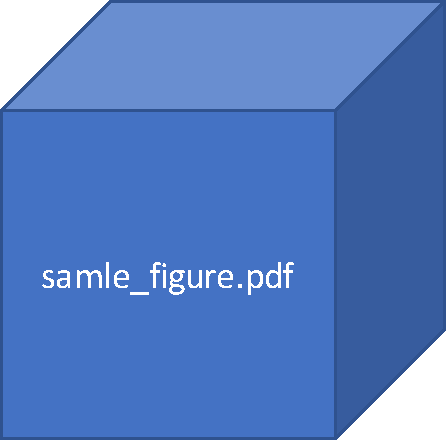
\includegraphics[width=0.5\hsize]{../figure/sample/sample_figure.pdf}
%   \caption{This is caption of sample figure.}
%   \label{Fig:Sample}
%  \end{center}
% \end{figure}

% \paragraph{Paragraph}

% \bibliographystyle{junsrt}
% \bibliography{}
\end{document}



\part{分子シミュレーションの解析方法}
\label{part:MDanalysis}
\documentclass[a4paper, 10.5pt, oneside, openany, uplatex]{jsarticle}

\author{山内 仁喬}
% 余白の設定.
% 参考文献:Latex2e 美文書作成入門, 14.3ページレイアウトの変更

% 行長の変更
\setlength{\textwidth}{40zw}           %全角40文字分

% 行間を制御するコマンド
\renewcommand{\baselinestretch}{0.9}

% 左マージンを変更
\setlength{\oddsidemargin}{25truemm}   % 左余白
\addtolength{\oddsidemargin}{-1truein} % 左位置デフォルトから-1inch

% 上マージンを変更
\setlength{\topmargin}{15truemm}       % 上余白
\addtolength{\topmargin}{-1truein}     % 上位置デフォルトから-1inch

% 本文領域の縦横の長さ変更
\setlength{\textheight}{242truemm}     % テキスト高さ: 297-(25+30)=242mm
\setlength{\textwidth}{160truemm}      % テキスト幅:  210-(25+25)=160mm
\setlength{\fullwidth}{\textwidth}     % ページ全体の幅


% 図・表の個数などの設定.
%% 図・表を入りやすさを制御するパラメーター
\setcounter{topnumber}{4}
\setcounter{bottomnumber}{4}
\setcounter{totalnumber}{4}
\setcounter{dbltopnumber}{3}
\setcounter{tocdepth}{1} % 項レベルまで目次に反映させるコマンド.
\renewcommand{\topfraction}{.95}
\renewcommand{\bottomfraction}{.90}
\renewcommand{\textfraction}{.05}
\renewcommand{\floatpagefraction}{.95}

% 使用するパッケージを記述.
\usepackage{amsmath} % 複雑な数式を使うときに便利
\usepackage{dcolumn}
\usepackage{color}
\usepackage{tabularx, dcolumn}
\usepackage{bm} % 数式環境内で太字を使うときに便利.
\usepackage{subcaption}  % 関連した複数の図を並べる時に使う
\usepackage[dvipdfmx]{graphicx} % 画像を挿入したり,テキストや図の拡大縮小・回転を行う.
\usepackage{verbatim} % 入力どおりの出力を行う.
\usepackage{makeidx} % 索引を作成できる.
\usepackage{dcolumn} % 表の数値を小数点で桁を揃える.
\usepackage{lscape} % 図表を90度横に倒して配置する.
\usepackage{setspace} % 行間調整.

\def\mbf#1{\mbox{\boldmath ${#1}$}}

% \newcolumntype{d}{D{+}{\,\pm\,}{4,5}}
% \newcolumntype{i}{D{+}{\,\pm\,}{-1}}
% \newcolumntype{.}{D{.}{.}{6,3}}

\begin{document}


\title{再重法(Reweighting Teqhnique)}

\maketitle
\section{単ヒストグラム再重法 (Single-Histogram Reweighting Techniques)}
単ヒストグラム最重法~\cite{Ferrenberg1988,Ferrenberg1989}を用いることで, あるパラメーターにおけるシミュレーショントラジェクトリーから, 他のパラメータにおける平均値を求めることができる. 
例えば, 温度$T$のシミュレーションから温度$T^{\prime}$における平均値を算出したり, マルチカノニカルシミュレーションの結果からある温度$T$における物理量の平均値を求めることが可能となる. 

\subsection{一般的な定式化}
ある重み$W(\lambda)$に基づく物理系を考える. 
パラメータ$\lambda$は例えばポテンシャルエネルギーなどであり, カノニカルアンサンブルの場合, $W(\lambda)$はボルツマン因子$W_{\mathrm{B}}(U) = e^{-U/k_{\mathrm{B}}T} = e^{-\beta U}$となる. 
パラメータ$\lambda$に関する系の状態密度$n(\lambda)$が分かっている場合, $\lambda$に関する確率分布と任意の物理量$A(\lambda)$の期待値は, 
\begin{alignat}{3}
    P(\lambda) &=
    \frac{n(\lambda)W(\lambda)}{\int d\lambda~ n(\lambda) W(\lambda)} &&=
    \frac{1}{Z} n(\lambda)W(\lambda)
    \label{Eq:ProbDist-Lambda}
    \\
    \langle A \rangle &=
    \frac{\int d\lambda~ A(\lambda)n(\lambda)W(\lambda)}{\int d\lambda~ n(\lambda) W(\lambda)} &&=
    \frac{1}{Z} \int d\lambda~ A(\lambda)n(\lambda)W(\lambda)
    \label{Eq:PhysAverage-Lambda}
\end{alignat}
と計算される. ここで, $Z$は分配関数である. 
系の状態密度が分かっていれば, 確率分布や物理量の期待値を得ることができる. 
しかし, 一般には系の状態密度は厳密には分かっていないため, 確率分布や物理量の期待値を計算するには分子シミュレーションを実行して状態密度を推定する必要がある. 

分子シミュレーションを実行して, $h$個のサンプルを得たとする. 
$\lambda$に関する確率分布は, 分子シミュレーションによって得られるパラメータ$\lambda$のヒストグラム$H(\lambda)$を用いて, 
\begin{equation}
    P(\lambda) = H(\lambda) / h
\end{equation}
と推定することができる. したがって, 式(\ref{Eq:ProbDist-Lambda})より, 状態密度は
\begin{equation}
    n(\lambda) = Z \frac{P(\lambda)}{W(\lambda)} = Z \frac{H(\lambda)}{h W(\lambda)}
    \label{Eq:Density-of-states-W}
\end{equation}
と推定できる. また, 物理量$A$の期待値は, 式(\ref{Eq:PhysAverage-Lambda})より
\begin{align}
    \langle A \rangle &=
    \frac{1}{Z} \int d\lambda A(\lambda) n(\lambda) W(\lambda) \\ &=
    \frac{1}{Z} \int d\lambda A(\lambda) Z \frac{P(\lambda)}{W(\lambda)} W(\lambda) \\ &=
    \int d\lambda A(\lambda) H(\lambda)/h
\end{align}
と計算できる. 

続いて, 重み$W(\lambda)$に基づいた分子シミュレーションのトラジェクトリーを用いて, 重み$W^{\prime}(\lambda)$に基づいた統計アンサンブルの確率分布と物理量の期待値を推定することを考える. 
この時, 確率分布と物理量の平均値は, 
\begin{alignat}{3}
    P(\lambda) &=
    \frac{n(\lambda)W^{\prime}(\lambda)}{\int d\lambda~ n(\lambda) W^{\prime}(\lambda)} &&=
    \frac{1}{Z} n(\lambda)W^{\prime}(\lambda)
    \label{Eq:ProbDist-Lambda-Prime}
    \\
    \langle A \rangle &=
    \frac{\int d\lambda~ A(\lambda)n(\lambda)W^{\prime}(\lambda)}{\int d\lambda~ n(\lambda) W^{\prime}(\lambda)} &&=
    \frac{1}{Z} \int d\lambda~ A(\lambda)n(\lambda)W^{\prime}(\lambda)
    \label{Eq:PhysAverage-Lambda-Prime}
\end{alignat}
と表される. 重み$W(\lambda)$に基づいた分子シミュレーションで得られた状態密度(\ref{Eq:Density-of-states-W})を代入すると, 
確率分布は, 
\begin{align}
    P(\lambda) =
    \frac{n(\lambda) W^{\prime}(\lambda)}{\int d\lambda~ n(\lambda) W^{\prime}(\lambda)} &=
    \frac{Z \frac{P(\lambda)}{W(\lambda)} W^{\prime}(\lambda)}{\int d\lambda~ Z \frac{P(\lambda)}{W(\lambda)} W^{\prime}(\lambda)} \\ &=
    \frac{\left\{H(\lambda)/W(\lambda)\right\} W^{\prime}(\lambda)}{\int d\lambda~ \left\{H(\lambda)/W(\lambda)\right\} W^{\prime}(\lambda)}
\end{align}
と推定することができる. 同様にして, 物理量の期待値は
\begin{align}
    \langle A \rangle  =
    \frac{\int d\lambda~ A(\lambda)\left\{H(\lambda)/W(\lambda)\right\} W^{\prime}(\lambda)}{\int d\lambda~ \left\{H(\lambda)/W(\lambda)\right\} W^{\prime}(\lambda)}
\end{align}
と推定できる. 

\subsection{カノニカルシミュレーションの場合}
温度$T$におけるカノニカルシミュレーションを実行し, $h$個のサンプルを得たとする. 
この時, ポテンシャルエネルギー$U$の確率分布は, 
\begin{equation}
    P_{NVT}(U;~T) = \frac{n(U)e^{-\beta U}}{\int dU~ n(U)e^{-\beta U}} = \frac{n(U)e^{-\beta U}}{Z(T)}
    \label{Eq:ProbDist-Potential-NVT}
\end{equation}
であり, 物理量の期待値は
\begin{equation}
    \langle A \rangle_{T} = \frac{\int dU~A(U)n(U)e^{-\beta U}}{Z(T)}
\end{equation}
である. ここで, $\beta = 1/k_{\mathrm{B}}T$, $k_{\mathrm{B}}$はボルツマン定数, $n(U)$は状態密度, $Z(T)$は分配関数である. 
式(\ref{Eq:ProbDist-Potential-NVT})より, 状態密度は
\begin{equation}
    n(U) = Z(T) P_{NVT}(U;~T) / e^{-\beta U}
\end{equation}
とかける. 通常, 状態密度は事前に分からないことが多く, シミュレーションを実行することで, はじめて系の状態密度を推定することができる. 
確率分布は, シミュレーションで得られたポテンシャル$U$のヒストグラム$H(U)$に比例し, 
\begin{equation}
    P_{NVT}(U;~T)= H(U)/h
\end{equation}
と書くことができる. したがって, 状態密度は
\begin{equation}
    n(U) = \frac{Z(T) H(U)}{he^{-\beta U}}
    \label{Eq:Density-of-states}
\end{equation}
と計算することができる. 
一方, 温度$T^{\prime}=1/k_{\mathrm{B}}\beta^{\prime}$における確率分布は
\begin{equation}
    P_{NVT}(U;~T^{\prime}) =
    \frac{n(U)e^{-\beta^{\prime} U}}{\int dU~ n(U)e^{-\beta^{\prime} U}}
\end{equation}
とかける. ここに温度$T$のカノニカルシミュレーションで得られた状態密度の式(\ref{Eq:Density-of-states})を代入すると, 
\begin{align}
    P_{NVT}(U;~T^{\prime}) &=
    \frac{\frac{Z(T) H(U)}{he^{-\beta U}} e^{-\beta^{\prime} U}}{\int dU~ \frac{Z(T) H(U)}{he^{-\beta U}}e^{-\beta^{\prime} U}} \\ &=
    \frac{\left\{H(U)/e^{-\beta U}\right\} e^{-\beta^{\prime} U}}{\int dU~ \left\{H(U)/e^{-\beta U}\right\}e^{-\beta^{\prime} U}} \\ &=
    \frac{H(U) e^{-U(\beta^{\prime} -\beta)}}{\int dU~ H(U) e^{-U(\beta^{\prime} -\beta)}}
\end{align}
を得る. また, 物理量の期待値は
\begin{equation}
    \langle A \rangle_{T^{\prime}} = \frac{\int dU~ A(U) H(U) e^{-U(\beta^{\prime} -\beta)}}{\int dU~ H(U) e^{-U(\beta^{\prime} -\beta)}}
\end{equation}
とかける. 
このように, 温度$T$のサンプルからの温度$T^{\prime}$における確率分布を推定式を得ることができる. 
一般的には, $T^{\prime}$が$T$近傍の値の時は比較的精度良く推定することができ, $T$と$T^{\prime}$の値が離れるにつれて, 推定された物理量の精度は悪くなってしまう. 


\section{多ヒストグラム再重法 (WHAM: Weighted Histogram Analysis Method)}

\subsection{WHAM方程式の導出}
WHAMを用いることで, $M$個のシミュレーションで得られたサンプルから, 任意のパラメータ設定における確率分布$P$についての最適な推定方法を得ることができる. 
ここでは, カノニカルシミュレーションの場合を考えていく. $m$番目のシミュレーションは温度$T_{m}=1/(k_{\mathrm{B}}\beta_{m})$で実行され, そこで得られたサンプルの数を$N_{m}$と表すことにする. 

\subsubsection{相関のある時系列データの統計的不確かさの評価法}
ここでは, 相関のある時系列データの統計的不確かさについて簡単にまとめる~\cite{Janke2002,Chodera2007}. 
定常で時間可逆な確率過程からサンプルされた観測量$A$について, データ間で相関のあるような連続した観測量の時系列$\{A_{i}\}_{i=1}^{N}$を考える. 
期待値$\langle A \rangle$は単純な算術平均で推定することができる:
\begin{equation}
    \hat{A} =
    \bar{A} =
    \frac{1}{N}\sum_{i=1}^{N} A_{i}
\end{equation}
上付きの$\hat{}$で推定値であることを表す. 
また, 上付きの$\bar{}$は算術平均であることを表す. 
ここでは$\langle A \rangle$と$\bar{A}$を区別して考える. 
$\langle A \rangle$は常数であり, 何かある値に求められるようなものである. 
一方, $\bar{A}$は期待値$\langle A \rangle$の推定値であるため, 取りうる値は期待値周辺を揺らぐ. 

ある物理量$A$の推定値$\hat{A}$について, 統計的不確かさについて考える. 
統計的不確かさは
\begin{align}
    \delta^{2} \hat{A} &\equiv
    \left\langle \left( \hat{A} - \langle \hat{A}\rangle \right)^{2} \right\rangle
    = \langle \hat{A}^{2} \rangle - \langle \hat{A} \rangle^{2}
    \notag \\ &=
    \frac{1}{N^{2}} \sum_{i,j=1}^{n} \langle A_{i} A_{j} \rangle -
    \frac{1}{N^{2}} \sum_{i,j=1}^{n} \langle A_{i} \rangle \langle A_{j} \rangle
\end{align}
と計算される. 
対角部分と非対角部分に分割すると, 
\begin{align}
    \delta^{2} \hat{A} =
    \frac{1}{N^{2}} \sum_{i=1}^{n}
    \left(\langle A_{i}^{2} \rangle - \langle A_{i}\rangle^{2} \right) +
    \frac{1}{N^{2}} \sum_{i \neq j = 1}^{n}
    \left(\langle A_{i}A_{j} \rangle - \langle A_{i}\rangle \langle A_{j}\rangle \right)
\end{align}
となる. 右辺第一項は観測量の分散に$1/N$を乗じたものであり, 右辺第二項は観測量の相関である. 
第二項について$i$と$j$の対称性を考えると, 和は$\sum_{i \neq j} = 2\sum_{i=1}^{N} \sum_{j=i+1}^{N}$とすることができる. さらに$k=|i-j|$を定めると, $i$と$j$に関する和は$k$についての和に置き直すことができる:
\begin{align}
    \sum_{i \neq j = 1}^{N}
    \left(\langle A_{i}A_{j} \rangle - \langle A_{i}\rangle \langle A_{j}\rangle \right)
    &=
    2\sum_{i=1}^{N} \sum_{j=i+1}^{N}
    \left(\langle A_{i}A_{j} \rangle - \langle A_{i}\rangle \langle A_{j}\rangle \right)
    \\
    &=
    2\sum_{k=1}^{N-1}
    \left(
        \langle A_{i}A_{i+k} \rangle - \langle A_{i}\rangle \langle A_{i+k}\rangle
    \right)
    \left( N - k \right)
\end{align}
ここで$(N-k)$は, ある$k$について$i<j$の時, $|i-j| = k$となるような整数の組の数に由来する. 
以上より, 統計的不確かさは
\begin{align}
    \delta^{2} \hat{A} &=
    \frac{1}{N}
    \left(\langle A_{i}^{2} \rangle - \langle A_{i}\rangle^{2} \right) +
    \frac{2}{N} \sum_{k=1}^{N-1}
    \frac{N-k}{N}
    \left(
        \langle A_{i}A_{i+k} \rangle - \langle A_{i}\rangle \langle A_{i+k}\rangle
    \right)
    \\
    &\equiv
    \frac{\sigma_{A}^{2}}{N} (1+2\tau)
    \\
    &\equiv
    \frac{\sigma_{A}^{2}}{N/g}
    \label{Eq:Statistical-Uncertainty-A}
\end{align}
と計算される. ここで, $\sigma_{A}^{2}$は分散, $g$は統計的非効率性因子, $\tau$は自己相関時間であり, それぞれ
\begin{align}
    \sigma_{A}^{2} &\equiv \langle A_{i}^{2} \rangle - \langle A_{i} \rangle^{2}
    \\
    \tau           &\equiv \sum_{k=1}^{N-1}\left(1 - \frac{k}{N}\right)C_{k}
    \\
    g              &\equiv 1 + 2\tau
\end{align}
と定義した. また$C_{k}$は
\begin{equation}
    C_{k} \equiv
    \frac{\langle A_{i} A_{i+k}\rangle - \langle A_{i} \rangle^{2}}{\langle A_{i}^{2} \rangle - \langle A_{i} \rangle^{2}}
\end{equation}
で定義される, 規格化された自己相関関数である. 
統計的非効率因子$g=1+2\tau$は1以上の値をもつ. $N/g$は時系列データに含まれる有効サンプル数(非相関データの数)を与える. 
$g$の値はシミュレーションにおいてサンプルを取得する時間ステップ間隔に依存する. 
より長い時間ステップ間隔でサンプリングすれば, $g$の値は1に近づく. 

\subsubsection{ヒストグラムの数学的定式化}
指示関数$\chi_{l}(A)$を, 観測量$A$が中心値$A_{l}$, 幅$\Delta A$のビンに含まれるかどうかを判定する関数として, 次のように定義する:
\begin{equation}
    \chi_{l}(A) =
    \begin{cases}
        1 ~~~~\text{if}~ X \in [A_{l} - \frac{\Delta A}{2},~ A_{l} + \frac{\Delta A}{2}) \\
        0 ~~~~\text{otherwise}
    \end{cases}
\end{equation}
ここで, $l$は$A$を離散化した時のビン番号を表す. また, 
$m$番目のシミュレーションの$n$番目の観測量を$A_{mn}$とすると, 指示関数の時系列は$\{\chi_{l}(A_{mn})\}_{n=1}^{N_m}$と表せる. 
$N_{m}$は$m$番目のシミュレーションのサンプル数である. 
$m$番目のシミュレーションに対する観測量$A_k$に関するヒストグラム$H_{m}$は
\begin{equation}
    H_{m}(A_{l}) = \sum_{n=1}^{N_m} \chi_{l}(A_{mn})
\end{equation}
と計算され, 全てのシミュレーションに渡って観測量をカウントしたヒストグラム$H$は
\begin{equation}
    H(A_{l}) = \sum_{m=1}^{M} \sum_{n=1}^{N_m} \chi_{l}(A_{mn})
\end{equation}
と計算することができる. 

\subsubsection{ヒストグラムの統計的不確かさ}
$m$番目のシミュレーションのヒストグラムは, 
\begin{equation}
    H_{m}(A_{l}) =
    \sum_{n=1}^{N_m} \chi_{l}(A_{mn}) =
    N_{m} \frac{1}{N_{m}} \sum_{n=1}^{N_m} \chi_{l}(A_{mn}) =
    N_{m} \hat{\chi}_{lm}
\end{equation}
と表すことができる. 統計的不確かさの式(\ref{Eq:Statistical-Uncertainty-A})より, 
\begin{align}
    \delta^{2} H_{m}(A_{l}) &=
    \delta^{2} \{N_{m} \hat{\chi}_{lm}\} =
    N_{m}^{2} \delta^{2} \hat{\chi}_{lm} =
    N_{m}^{2} \frac{\sigma_{\chi}}{N_{m}/g}
\end{align}
と書き下せる. これを具体的に計算すると, 
\begin{align}
    \delta^{2} H_{m}(A_{l}) &=
    \frac{g_{m}}{N_{m}} N_{m}^{2}
    \left(
        \langle \chi_{lm}^{2} \rangle - \langle \chi_{lm} \rangle^{2}
    \right)
    \\ &=
    \frac{g_{m}}{N_{m}} N_{m}^{2}
    \left(
        \langle \chi_{lm} \rangle - \langle \chi_{lm} \rangle^{2}
    \right)
    \\ &=
    g_{m} N_{m} \langle \chi_{lm} \rangle
    \left(1 - \langle \chi_{lm} \rangle \right)
    \\ &=
    g_{m} \langle H_{m}(A_{l}) \rangle
    \left(1 - \frac{\langle H_{m}(A_{l}) \rangle}{N_{m}} \right)
\end{align}
と計算される. 
ここで, $\chi_{lm}$は指示関数のため$\left[\chi_{l}(A_{m})\right]^{2} = \chi_{l}(A_{m})$であることを用いた. ヒストグラムの分布が疎であり, 十分な数のビンを用いている場合, $\langle H_{m}(A_{l})\rangle/N_{m} << 1$となるので, 
\begin{equation}
    \delta^{2} H_{m}(A_{l}) \simeq g_{m} \langle H_{m}(A_{l}) \rangle
    \label{Eq:Statistical-Uncertainty-Histogram}
\end{equation}
と近似することができる. 


\subsubsection{各シミュレーションの状態密度の推定}
ここでは, $m$番目のシミュレーションに対する状態密度$\Omega_{m}(U)$の推定方法を考える. 
そのためには, 確率密度分布を数学的に表現する方法が必要である. 
J.~D.~Choderaら\cite{Chodera2007}が指摘しているように, 確率密度分布の推定にノンパラメトリックを用いることもできるが, 
ここではより簡便な, Kumar\cite{Kumar1992}らやFerrenbergとSwendsen\cite{Ferrenberg1989b}が提案したヒストグラムに基づいた確率分布の推定方法を説明する. 

まず, カノニカルアンサンブルにおけるポテンシャルの確率分布は, 
\begin{align}
    P_{NVT}(U;~T_{m})
    =
    \frac{\Omega_{m}(U) e^{-\beta_{m}U}}{\int dU~\Omega_{m}(U)e^{-\beta_{m}U}}
    &=
    \frac{1}{Z(\beta_{m})} \Omega_{m}(U) e^{-\beta_{m}U}
    \\
    &=
    \Omega_{m}(U) \exp[f_{m} - \beta_{m}U]
    \label{Eq:WHAM-ProbDist-NVT}
\end{align}
と書くことができる. ここで, $Z_{m}(\beta_{m})$は分配関数であり, ヘルムホルツの自由エネルギー$F_{m}$あるいは無次元化されたヘルムホルツの自由エネルギー$f_{m}$を用いて
\begin{equation}
    Z(\beta_{m}) = e^{-\beta_{m}F_{m}} = e^{-f_{m}}
\end{equation}
と書かれることを用いた. 

続いて, シミュレーションで得られたサンプルから得られるヒストグラム$H$に基づいた確率分布の推定を考える. 
ヒストグラムを用いるとポテンシャルの確率分布は, 
\begin{equation}
    P_{NVT}(U_{l};~T_{m}) =
    \Omega_{m}(U) \exp[f_{m} - \beta_{m}U_{l}]
    \simeq
    \frac{1}{\Delta U} \frac{H_{m}(U_{l})}{N_{m}}
\end{equation}
のように見積もることができるため, 状態密度をヒストグラムを用いて
\begin{equation}
    \hat{\Omega}_{m}(U_{l}) =
    \frac{H_{m}(U_{l})}{N_{m}\Delta U \exp[f_{m}-\beta_{m}U_{l}]}
    \label{Eq:Density-of-States-Mth}
\end{equation}
と推定することができる. 


\subsubsection{状態密度の最良推定値$\hat{\Omega}(U)$の表現方法}

状態密度$\hat{\Omega}(U_{l})$の最良推定値を, $M$個のシミュレーションに対する状態密度の推定値$\hat{\Omega}_{m}(U)~~(m = 1,\ldots, M)$の重み付きの和で表す:
\begin{equation}
    \hat{\Omega}(U_{l}) = \sum_{m=1}^{M} w_{m}(U_{l}) \hat{\Omega}_{m}(U_{l})
    \label{Eq:WHAM-Estimation-Density-of-States}
\end{equation}
ここで, 重み$w_{i}$は拘束条件
\begin{equation}
    \sum_{m=1}^{M} w_{m}(U_{l}) =1
    \label{Eq:WHAM-Weight-Constrain}
\end{equation}
を満たす. 
WHAMでは, 状態密度$\hat{\Omega}(U_{l})$の最良推定値を得るような重み$w_{i}$の集合は, 状態密度の統計誤差$\delta^{2}\hat{\Omega}(U_{l})$を最小化することによって導出する. 
状態密度の統計誤差は具体的に, 
\begin{align}
    \delta^{2}\hat{\Omega}(U_{l}) &=
    \left[\hat{\Omega}(U_{l}) - \langle \hat{\Omega}(U_{l}) \rangle \right]^{2}
    \\ &=
    \left[
        \sum_{m=1}^{M} w_{m}(U_{l}) \hat{\Omega}_{m}(U_{l}) -
        \left\langle \sum_{m=1}^{M} w_{m}(U_{l}) \hat{\Omega}_{m}(U_{l}) \right\rangle
    \right]^{2}
    \\ &=
    \sum_{m=1}^{M} w_{m}^{2}(U_{l})
    \left[
        \hat{\Omega}_{m}(U_{l}) -
        \left\langle \hat{\Omega}_{m}(U_{l}) \right\rangle
    \right]^{2}
    \\ &=
    \sum_{m=1}^{M} w_{m}^{2}(U_{l}) \delta^{2}\hat{\Omega}_{m}(U_{l})
\end{align}
と計算される. 各シミュレーションの状態密度(\ref{Eq:Density-of-States-Mth})より
\begin{equation}
    \delta^{2} \hat{\Omega}_{m}(U_{l}) =
    \frac{\delta^{2}H_{m}(U_{l})}{\{N_{m} \Delta U \exp[f_{m} -\beta_{m}U_{l}]\}^{2}}
    \label{Eq:WHAM-Density-of-State-Mth-Estimation}
\end{equation}
であるので, 
\begin{equation}
    \delta^{2}\hat{\Omega}(U_{l}) =
    \sum_{m=1}^{M} w_{m}^{2}(U_{l})
    \frac{\delta^{2}H_{m}(U_{l})}{\{N_{m} \Delta U \exp[f_{m} -\beta_{m}U_{l}]\}^{2}}
\end{equation}
と表すことができる. 
このように, $\delta^{2}\hat{\Omega}(U_{l})$は, $M$個の見積もられた状態密度$\hat{\Omega}_{1}(U_{l}),\ldots,\hat{\Omega}_{M}(U_{l})$の統計誤差$\delta^{2}\hat{\Omega}_{1}(U_{l}),\ldots,\delta^{2}\hat{\Omega}_{M}(U_{l})$に由来するので, 結局はヒストグラムの統計誤差$\delta^{2}H_{1}(U_{l}),\ldots,\delta^{2}H_{M}(U_{l})$に依存する形で書かれる. 
式(\ref{Eq:Statistical-Uncertainty-Histogram})を用いると, ヒストグラムの統計誤差をヒストグラムの期待値$\langle H_{m}(U_{l})\rangle$で近似できる. ヒストグラムの期待値は, 得られるべき状態密度の最良推定値で置き直すと, 
\begin{align}
    \langle H_{m}(U_{l}) \rangle &=
    N_{m} \Delta U P_{NVT}(U_{l};~T_{m}) \\ &\simeq
    N_{m} \Delta U \hat{\Omega(U_{l})} \exp[f_{m}-\beta_{m}U_{l}]
\end{align}
となるので, 式(\ref{Eq:Statistical-Uncertainty-Histogram})を用いてヒストグラムの統計誤差を
\begin{align}
    \delta^{2} H_{m}(U_{l}) \simeq
    g_{m} \langle H_{m}(U_{l})\rangle \simeq
    g_{m} N_{m} \Delta U \hat{\Omega(U_{l})} \exp[f_{m}-\beta_{m}U_{l}]
\end{align}
と計算することができる. 
これを式(\ref{Eq:WHAM-Density-of-State-Mth-Estimation})に代入することで, 各シミュレーションに対する状態密度の推定値の統計誤差$\hat{\Omega_{m}}$を
\begin{align}
    \delta^{2} \Omega_{m} (U_{l}) &=
    \frac{\delta^{2} H_{m} (U_{l})}{\{N_{m} \Delta U \exp[f_{m} -\beta_{m}U_{l}]\}^{2}}
    % \\ &=
    % \frac{g_{m} N_{m} \Delta U \hat{\Omega(U_{l})} \exp[f_{m}-\beta_{m}U_{l}]}{\{N_{m} \Delta U \exp[f_{m} -\beta_{m}U_{l}]\}^{2}}
    % \\ &=
    % \frac{g_{m}\hat{\Omega(U_{l})}}{N_{m} \Delta U \exp[f_{m} -\beta_{m}U_{l}]}
    \\ &=
    \frac{\hat{\Omega(U_{l})}}{g_{m}^{-1}N_{m} \Delta U \exp[f_{m} -\beta_{m}U_{l}]}
    \label{Eq:WHAM-Density-of-States-Mth-Estimation}
\end{align}
と推定することができる. 


\subsubsection{重み$w_{i}$の決定: Lagrangeの未定乗数法}
状態密度の統計誤差$\delta^{2}\hat{\Omega}(U_{l})$が拘束条件(\ref{Eq:WHAM-Weight-Constrain})の下で最小になるような重み$w_{i}$の集合を得るために, Lagrangeの未定乗数法を用いる. ラグランジュ関数は
\begin{align}
    \mathcal{L} =
    \delta^{2}\hat{\Omega}(U_{l}) -
    \alpha \left[\sum_{m=1}^{M}w_{i}(U_{l}) - 1\right] =
    \left[\sum_{m=1}^{M} w_{m}^{2}(U_{l}) \delta^{2}\hat{\Omega}_{m}(U_{l}) \right] -
    \alpha \left[\sum_{m=1}^{M}w_{i}(U_{l}) - 1\right]
\end{align}
とかける. 
極値をとる条件$\partial \mathcal{L}/\partial \alpha = 0$, $\partial \mathcal{L}/\partial w_{m} = 0$より, 
\begin{align}
    \frac{\partial \mathcal{L}}{\partial \alpha} &=
    \sum_{m=1}^{M} w_{m}(U_{l}) - 1 = 0
    \\
    \frac{\partial \mathcal{L}}{\partial w_{m}} &=
    2 w_{m}(U_{l}) \delta^{2} \hat{\Omega}_{m}(U_{l}) - \alpha = 0
    \label{Eq:WHAM-Lagrange-Partial2}
\end{align}
を得る. 式(\ref{Eq:WHAM-Lagrange-Partial2})より, 
\begin{equation}
    \alpha =
    2 w_{1} (U_{l}) \delta^{2} \hat{\Omega}_{1} (U_{l}) =
    2 w_{2} (U_{l}) \delta^{2} \hat{\Omega}_{2} (U_{l}) =
    \ldots
    2 w_{M} (U_{l}) \delta^{2} \hat{\Omega}_{M} (U_{l})
\end{equation}
であるので, これを拘束条件(\ref{Eq:WHAM-Weight-Constrain})に代入すると
\begin{equation}
    w_{1}(U_{l}) +
    \frac{\delta^{2} \hat{\Omega}_{1}(U_{l})}{\delta^{2} \hat{\Omega}_{2}(U_{l})} w_{1}(U_{l}) +
    \frac{\delta^{2} \hat{\Omega}_{1}(U_{l})}{\delta^{2} \hat{\Omega}_{3}(U_{l})} w_{1}(U_{l}) +
    \ldots
    \frac{\delta^{2} \hat{\Omega}_{1}(U_{l})}{\delta^{2} \hat{\Omega}_{M}(U_{l})} w_{1}(U_{l}) =
    1
\end{equation}
を得る. これより, 
\begin{align}
    w_{1}(U_{l}) &=
    \frac
    {1}
    {\left\{
        \frac{1}{\delta^{2}\hat{\Omega}_{1}(U_{l})} +
        \frac{1}{\delta^{2}\hat{\Omega}_{2}(U_{l})} +
        \ldots
        \frac{1}{\delta^{2}\hat{\Omega}_{M}(U_{l})}
    \right\} \delta^{2}\hat{\Omega}_{1}(U_{l})
    }
    =
    \frac
    {\frac{1}{\delta^{2}\hat{\Omega}_{1}(U_{l})}}
    {\left\{\sum_{m=1}^{M} \frac{1}{\delta^{2}\hat{\Omega}_{m}(U_{l})}\right\}}
\end{align}
と計算される. 
その他の重みも同様に得ることができる:
\begin{align}
    w_{i}(U_{l}) =
    \frac
    {\frac{1}{\delta^{2}\hat{\Omega}_{m}(U_{l})}}
    {\left\{\sum_{m=1}^{M} \frac{1}{\delta^{2}\hat{\Omega}_{m}(U_{l})}\right\}}
    \label{Eq:WHAM-Weight}
\end{align}

\subsubsection{状態密度$\Omega(U)$の推定}
得られた重み(\ref{Eq:WHAM-Weight})と各シミュレーションに対する状態密度の推定値の統計誤差(\ref{Eq:WHAM-Density-of-States-Mth-Estimation})を用いると, 状態密度の推定値(\ref{Eq:WHAM-Estimation-Density-of-States})は
\begin{align}
    \hat{\Omega(U_{l})}
    &=
    \sum_{m=1}^{M} w_{m}(U_{l}) \hat{\Omega_{m}(U_{l})}
    \\ &=
    \sum_{m=1}^{M}
    \frac
    {
        [\delta^{2}\hat{\Omega}_{m}(U_{l})]^{-1} \hat{\Omega_{m}(U_{l})}
    }
    {
        [\sum_{i=1}^{M}\delta^{2}\hat{\Omega}_{i}(U_{l})]^{-1}
    }
    \\ &=
    \sum_{m=1}^{M}
    \frac
    {
        \frac{g_{m}^{-1}N_{m}\Delta U \exp[f_{m}-\beta_{m}U_{l}]}{\hat{\Omega}(U_{l})}
        \frac{H_{m}(U_{l})}{N_{m}\Delta U \exp[f_{m}-\beta_{m}U_{l}]}
    }
    {
        \left[
            \sum_{i=1}^{M}
            \frac{g_{i}^{-1} N_{i} \Delta U \exp[f_{i}-\beta_{i}U_{l}]}{\hat{\Omega}(U_{l})}
        \right]
    }
    \\ &=
    \sum_{m=1}^{M}
    \frac{g_{m}^{-1} H_{m}(U_{l})}{\sum_{i=1}^{M} g_{i}^{-1} N_{i} \Delta U \exp[f_{i}-\beta_{i}U_{l}]}
\end{align}
と計算できる. 

\subsubsection{確率分布と物理量の平均値}
以上より, 確率分布は
\begin{align}
    P(U_{l};~ T) =
    \hat{\Omega(U_{l})} e^{-\beta U_{l}}
    =
    \sum_{m=1}^{M}
    \frac{g_{m}^{-1} H_{m}(U_{l}) e^{-\beta U_{l}}}{\sum_{i=1}^{M} g_{i}^{-1} N_{i} \Delta U \exp[f_{i}-\beta_{i}U_{l}]}
\end{align}
と計算される. ここで, 各シミュレーションに対する無次元化されたヘルムホルツの自由エネルギーは
\begin{align}
    e^{-f_{m}} =
    \sum_{l} \hat{\Omega}(U_{l}) e^{-\beta U_{l}} =
    \sum_{l} P(U_{l};~ T)
\end{align}
である. また, 物理量の平均値は
\begin{equation}
    \left\langle A \right\rangle_{T} =
    \sum_{l}
    \frac{A(U_{l}) P(U_{l};~ T)}{P(U_{l};~ T)}
\end{equation}
で計算することができる. 

\subsection{WHAM法のまとめ: カノニカルアンサンブルの場合}
カノニカルアンサンブルにおける物理量$A(U)$の平均値は, 
\begin{equation}
    \langle T \rangle_{T} =
    \frac{\int dU~A(U) \omega(U) e^{-\beta U}}{\int dU~\omega(U) e^{-\beta U}}
\end{equation}
と計算できる. 
WHAMを用いることで, $M$個のシミュレーションで得られたサンプルを用いて系の状態密度を見積もることができる. 
ここで$k$番目のシミュレーションは温度$\beta_{k} = 1 / k_{\mathrm{B}} T_{k}$で実行されたカノニカルシミュレーションとする. 
また, $k$番目のシミュレーションで得られたサンプル数を$h_{k}$とする. 
状態密度$\Omega(U)$は, 無次元化されたヘルムホルツの自由エネルギー$f_{i}$を用いて, 
\begin{align}
    \Omega(U;~T) &=
    \frac{\sum_{m=1}^{M} g_{m} H_{m}(U)}{\sum_{m=1}^{M} g_{m} N_{m} e^{f_{m} - \beta_{m} U}}
    \label{Eq:WHAM-Density-of-states}
    \\
    e^{-f_{m}} &=
    \sum_{U} \Omega (U;~T_{m}) e^{-\beta_{m}U}
    \label{Eq:WHAM-Helmholtz-Free-Energy}
\end{align}
である. ここで, $H_{i}(U)$は$i$番目のシミュレーションによって得られた, ポテンシャルエネルギー$U$に関するヒストグラム, $f_{i} = \beta_{i} F_{i}$は無次元化されたヘルムホルツの自由エネルギーである. 
式(\ref{Eq:WHAM-Density-of-states})と式(\ref{Eq:WHAM-Helmholtz-Free-Energy})を自己無撞着に解くことで, 系の状態密度を推定することができる. 
$f_{i}$の値のセットの初期値は任意に取ることができるので, 全ての$f_{i}$に対して0としても大丈夫である. 

\section{多状態ベネット受容比法 (MBAR: Multistate Bennett Acceptance Ratio Estimator)}
\subsection{熱平衡状態の表式}
$K$個の同じ熱力学平衡状態(例えば, $NVT$, $NPT$, $\mu NT$アンサンブルなど)から$N_{i}$個の相関のないサンプルを得たとする. 
各サンプルに対する状態は, 用いたアンサンブルに応じて, 逆温度$\beta$, ポテンシャルエネルギー$U$, 圧力$p$, 化学ポテンシャル$\mu$などにより特徴づけられる. 
ここで, 熱平衡状態$i$に対する無次元ポテンシャル関数$u_{i}(\bm{x})$を
\begin{equation}
    u_{i}(\bm{x}) =
    \beta_{i}
    \left[
        U_{i}(\bm{x}) + p_{i}V(\bm{x}) + \bm{\mu}_{i}^{t} \bm{n}(\bm{x})
    \right]
\end{equation}
と定義する. 
ここで, $\bm{x} \in \Gamma$は位相空間$\Gamma$内の系の構造を表す. 
また, $V(\bm{x})$は体積(定圧アンサンブルの場合), $\bm{n}(\bm{x})$は$M$成分系における各成分の分子の数(グランドカノニカルアンサンブルの場合)を表す. 
アンブレラサンプリングなどバイアスポテンシャルを課している場合, $U$の中にはそのようなバイアスポテンシャルも含まれることに注意する. 

熱平衡状態$i$から得られたサンプル$\left\{\bm{x}_{in}\right\}_{n=1}^{N_{i}}$は, 確率分布$p_{i}$
\begin{align}
    p_{i} (\bm{x}) =
    \frac{q_{i}(\bm{x})}{\int_{\Gamma} d\bm{x}~q_{i}(\bm{x})} =
    \frac{q_{i}(\bm{x})}{c_{i}}
\end{align}
にしたがっている. 
ここで, $q_{i}$は非負の規格化されていない密度関数であり, $c_{i}$は規格化定数(統計力学では分配関数)である. 規格化定数が一般的に事前に分かっているという状況は多くない. 
温度や圧力制御されたモンテカルロ法や分子動力学法で得られたサンプル, あるいは実験で得られたデータの場合, 関数$q_{i}$はボルツマン因子で表される:
\begin{equation}
    q_{i}(\bm{x}) = e^{-u_{i}(\bm{x})}
\end{equation}
ただし, マルチカノニカルシミュレーションなどの非ボルツマン因子に基づいたシミュレーションでは, このように表すことができないアンサンブルがあることにも注意する必要がある. 

\subsection{平衡状態間の自由エネルギー差と物理量の期待値の表式}
無次元化された自由エネルギー差は, 
\begin{equation}
    \Delta f_{ij} \equiv
    f_{j} - f_{i} =
    - \ln \frac{c_{j}}{c_{i}} =
    - \ln \frac{\int_{\Gamma} d\bm{x}~q_{j}(\bm{x})}{\int_{\Gamma} d\bm{x}~q_{i}(\bm{x})}
\end{equation}
である. ただし, $f_{i}$は次元を持つ自由エネルギー$F_{i}$と$f_{i} = \beta_{i} F_{i}$の関係で結ばれている. 

平衡状態$i$における物理量$A$の期待値は, 
\begin{equation}
    \langle A \rangle_{i} \equiv
    \int_{\Gamma} d\bm{x}~ p_{i}(\bm{x}) A(\bm{x}) =
    \frac{\int_{\Gamma} d\bm{x}~ A(\bm{x})q_{i}(\bm{x})}{\int_{\Gamma} d\bm{x}~ q_{i}(\bm{x})}
    \label{Eq:MBAR-Expectation-PhysVal}
\end{equation}
新たに密度関数$q(\bm{x})=A(\bm{x})q_{i}(\bm{x})$を定義すれば, 物理量の期待値は規格化定数の比で計算することができる. この時, $q(\bm{x})$はもはや非負である必要はない. 

\subsection{拡張ブリッジサンプリング推定法 (Extended Bridge Sampling Estimators)}
規格化定数$c_{i}$の比を推定する方法を構築する. 
恒等式$c_{i} \langle \alpha_{ij} q_{j} \rangle_{i} = c_{j} \langle \alpha_{ij} q_{i} \rangle_{j}$が成立することは
\begin{align}
    c_{i} \left\langle \alpha_{ij}q_{j} \right\rangle_{i} &=
    \left[\int_{\Gamma}d\bm{x}~ q_{i}(\bm{x})\right]
    \frac{\int_{\Gamma}d\bm{x}~ q_{i}(\bm{x}) \alpha_{ij}(\bm{x}) q_{j}}{\int_{\Gamma} d\bm{x} q_{i}(\bm{x})}
    \\ &=
    \int_{\Gamma}d\bm{x}~ q_{i}(\bm{x}) \alpha_{ij}(\bm{x}) q_{j}
    \\ &=
    \left[\int_{\Gamma}d\bm{x}~ q_{j}(\bm{x})\right]
    \frac{\int_{\Gamma}d\bm{x}~ q_{j}(\bm{x}) \alpha_{ij}(\bm{x}) q_{i}}{\int_{\Gamma} d\bm{x} q_{j}(\bm{x})}
    \\ &=
    c_{j} \left\langle \alpha_{ij}q_{i} \right\rangle_{j}
\end{align}
から分かる. $\alpha_{ij}(\bm{x})$はゼロでない$c_{i}$について任意に選べる関数である. 

この恒等式について両辺共に$j$について和をとる. 
期待値は$\langle g \rangle_{i}$は, 経験的に, $\sum_{n=1}^{N_{i}}g(\bm{x}_{in})$のように算術平均で推定することができることを用いれば, $i = 1,\ldots,K$に対してK個の方程式を得る:
\begin{equation}
    \sum_{j=1}^{K} \frac{\hat{c}_{i}}{N_{i}}
    \sum_{n=1}^{N_{i}} \alpha_{ij} q_{j}(\bm{x}_{in}) =
    \sum_{j=1}^{K} \frac{\hat{c}_{j}}{N_{j}}
    \sum_{n=1}^{N_{j}} \alpha_{ij} q_{i}(\bm{x}_{jn})
    \label{Eq:MBAR-EstimateEq-Partition-Function}
\end{equation}
ここで, 上付のハット$\hat{}$は推定値であることを示している. $i = 1,\ldots,K$について, 全ての$\hat{c}_{i}$に関する方程式の組みを解くことで, サンプルされたデータから$c_{i}$の推定値$\hat{c}_{i}$を得ることができる. 

$\alpha_{ij}(\bm{x})$には様々な選び方が可能であり, その中にはリウェイティングで一般的に使用されるものもある. MBAR法では, 可能な$\alpha_{ij}(\bm{x})$の選び方の中でも, 最も小さい分散を持つという意味において最適な$\alpha_{ij}(\bm{x})$を用いる. 
具体的には, 以下のような$\alpha_{ij}(\bm{x})$を採用する:
\begin{equation}
    \alpha_{ij}(\bm{x}) =
    \frac{N_{j}\hat{c}_{j}^{-1}}{\sum_{k=1}^{K}N_{k}\hat{c}_{k}^{-1}q_{k}(\bm{x})}
    \label{Eq:MBAR-Alpha-ij}
\end{equation}
この推定式は, 漸近不偏量であり, 唯一の解を持つことが保証されている. 
式(\ref{Eq:MBAR-EstimateEq-Partition-Function})と式(\ref{Eq:MBAR-Alpha-ij})からでは, $\hat{c}_{i}$の組について閉じた方程式を導けないため, 直接解くことができない. 
代わりに, 自己無撞着にあるいはNewton-Raphson法を用いて, 数値的にこの非線形方程式を解くことができる. 

サンプルの数が大きい範囲では, 一般的には比$\hat{c}_{i} / \hat{c}_{j}$の誤差は分散される. 
漸近的な共分散行列$\bm{\Theta} = \textrm{cov}(\ln c_{i},~\ln c_{j}) \equiv \textrm{cov}(\theta_{i},~\theta_{j})$は次のように推定される:
\begin{equation}
    \hat{\bm{\Theta}} =
    \bm{W}^{\mathrm{T}}
    \left(\bm{I}_{N} - \bm{W}\bm{N}\bm{W}^{\mathrm{T}}\right)^{+}
    \bm{W}
    \label{Eq:MBAR-Estimation-Variance-Covariance}
\end{equation}
ここで, $\bm{I}_{N}$は$N \times N$の単位行列, 
$N=\sum_{i=1}^{M}N_{i}$は全サンプル数, 
$\bm{N} = \mathrm{diag}(N_{1},~N_{2},~\ldots,N_{M})$は各シミュレーションのサンプル数を成分に持つベクトル, 
上付の$+$はMoore-Penroseのような一般化逆行列を表している. 
また, $\bm{W}$は$N \times K$の重み行列で, 
\begin{equation}
    W_{ni} =
    \hat{c}_{i}^{-1}
    \frac{q_{i}(\bm{x}_{n})}
    {\sum_{k=1}^{M} N_{k} \hat{c}_{k}^{-1} q_{k}(\bm{x}_{n})}
    \label{Eq:MBAR-Weight-Matrix}
\end{equation}
と計算される. ここで, サンプルは1つのラベル$n=1,\ldots,N$でラベル付けしている. 
したがって, サンプル$\bm{x}_{n}$が, どの分布$p(\bm{x})$からサンプルされているかは, もはや関係なくなっている. 
また, 上記の定義において, 
\begin{align}
    \sum_{n=1}^{N} W_{ni}       &= 1, ~~~~(i = 1,\ldots,K) \\
    \sum_{n=1}^{K} N_{i} W_{ni} &= 1, ~~~~(n = 1,\ldots,N)
\end{align}
を満たす. 
$\hat{\bm{\Theta}}$を見積もるとき, $N \times N$の擬逆行列を見積もる計算コストは, $K \times K$行列の固有値を見積もる計算コストまで減らすことが可能である. 多くの場合で, 共分散行列は$K \times K$行列の操作で見積もられる. 
規格化定数に対数をとった$\theta_{i}$に関する任意の関数
$\phi(\theta_{1},\ldots,\theta_{K})$と
$\psi(\theta_{1},\ldots,\theta_{K})$に関する推定値の共分散は
$\hat{\bm{\Theta}}$から見積もられる:
\begin{equation}
    \mathrm{cov}(\hat{\phi},~\hat{\psi}) =
    \sum_{i,j=1}^{K}
    \frac{\partial \phi}{\partial \theta_{i}}
    \hat{\theta}_{ij}
    \frac{\partial \psi}{\partial \theta_{j}}
\end{equation}

\subsection{無次元化された自由エネルギーの推定}
構造がボルツマン統計, すなわち$q_{i} \equiv \exp[-u_{i}(\bm{x})]$からサンプリングされた時, 式(\ref{Eq:MBAR-EstimateEq-Partition-Function})と式(\ref{Eq:MBAR-Alpha-ij})から, 以下のような無次元自由エネルギーの推定式が得られる:
\begin{equation}
    \hat{f}_{i} =
    -\ln \sum_{j=1}^{K} \sum_{n=1}^{N_{j}}
    \frac
    {\exp[-u_{i}(\bm{x}_{jn})]}
    {\sum_{k=1}^{K} N_{k} \exp[\hat{f}_{k} - u_{k}(\bm{x}_{jn})]}
    \label{Eq:MBAR-Dimensionless-Free-Energy}
\end{equation}
この推定式は$\hat{f}_{i}$に対して自己無撞着に解くことができる. 

推定された自由エネルギー差の不確かさは式(\ref{Eq:MBAR-Estimation-Variance-Covariance})と式(\ref{Eq:MBAR-Weight-Matrix})より
\begin{align}
    \delta^{2} \Delta \hat{f}_{ij}
    &\equiv
    \mathrm{cov}
    \left(
        - \ln \frac{\hat{c}_{j}}{\hat{c}_{i}},~
        - \ln \frac{\hat{c}_{j}}{\hat{c}_{i}},~
    \right)
    \\ &=
    \hat{\Theta}_{ii} - 2\hat{\Theta}{ij} + \hat{\Theta}_{ji}
\end{align}
と計算される. 

\subsubsection{無次元化された自由エネルギーの推定式の導出}
式(\ref{Eq:MBAR-EstimateEq-Partition-Function})と式(\ref{Eq:MBAR-Alpha-ij})から, 無次元自由エネルギーの推定式(\ref{Eq:MBAR-Dimensionless-Free-Energy})を導出する. 
式(\ref{Eq:MBAR-EstimateEq-Partition-Function})と式(\ref{Eq:MBAR-Alpha-ij})をもう一度書いておくと, それぞれ
\begin{equation}
    \sum_{j=1}^{K} \frac{\hat{c}_{i}}{N_{i}}
    \sum_{n=1}^{N_{i}} \alpha_{ij} q_{j}(\bm{x}_{in}) =
    \sum_{j=1}^{K} \frac{\hat{c}_{j}}{N_{j}}
    \sum_{n=1}^{N_{j}} \alpha_{ij} q_{i}(\bm{x}_{jn})
    \notag
\end{equation}
\begin{equation}
    \alpha_{ij}(\bm{x}) =
    \frac{N_{j}\hat{c}_{j}^{-1}}{\sum_{k=1}^{K}N_{k}\hat{c}_{k}^{-1}q_{k}(\bm{x})}
    \notag
\end{equation}
であった. ここで, 
\begin{align}
    q_{i}(\bm{x}) = e^{-u_{i}(\bm{x})}
    \\ \notag
    c_{i} = e^{-f_{i}}
    \notag
\end{align}
である. 
式(\ref{Eq:MBAR-Alpha-ij})を式(\ref{Eq:MBAR-EstimateEq-Partition-Function})に代入することで, 
\begin{align}
\begin{split}
    \sum_{j=1}^{K}
    \frac{\hat{c}_{i}}{N_{i}}
    \sum_{n=1}^{N_{i}}
    \frac{N_{j}\hat{c}_{j}^{-1}}{\sum_{k=1}^{K} N_{k} \hat{c}_{k}^{-1} q_{k}(\bm{x}_{in})}
    q_{j}(\bm{x}_{in})
    &=
    \sum_{j=1}^{K}
    \frac{\hat{c}_{j}}{N_{j}}
    \sum_{n=1}^{N_{j}}
    \frac{N_{j}\hat{c}_{j}^{-1}}{\sum_{k=1}^{K} N_{k} \hat{c}_{k}^{-1} q_{k}(\bm{x}_{jn})}
    q_{i}(\bm{x}_{jn})
    \\
    &=
    \sum_{j=1}^{K}
    \sum_{n=1}^{N_{j}}
    \frac{q_{i}(\bm{x}_{jn})}{\sum_{k=1}^{K} N_{k} \hat{c}_{k}^{-1} q_{k}(\bm{x}_{jn})}
\end{split}
\end{align}
さらに, 左辺について, 
\begin{align}
\begin{split}
    \sum_{j=1}^{K}
    \frac{\hat{c}_{i}}{N_{i}}
    \sum_{n=1}^{N_{i}}
    \frac{N_{j}\hat{c}_{j}^{-1}}{\sum_{k=1}^{K} N_{k} \hat{c}_{k}^{-1} q_{k}(\bm{x}_{in})}
    q_{j}(\bm{x}_{in})
    &=
    \frac{\hat{c}_{i}}{N_{i}}
    \sum_{j=1}^{K}
    \sum_{n=1}^{N_{i}}
    \frac{N_{j}\hat{c}_{j}^{-1}}{\sum_{k=1}^{K} N_{k} \hat{c}_{k}^{-1} q_{k}(\bm{x}_{in})}
    q_{j}(\bm{x}_{in})
    \\ &=
    \frac{\hat{c}_{i}}{N_{i}}
    \sum_{j=1}^{K}
    \left[
        \frac
        {N_{j}\hat{c}_{j}^{-1} q_{j}(\bm{x}_{i1})}
        {\sum_{k=1}^{K} N_{k} \hat{c}_{k}^{-1} q_{k}(\bm{x}_{i1})}
        + \ldots +
        \frac
        {N_{j}\hat{c}_{j}^{-1} q_{j}(\bm{x}_{i N_{i}})}
        {\sum_{k=1}^{K} N_{k} \hat{c}_{k}^{-1} q_{k}(\bm{x}_{i N_{i}})}
    \right]
    \\ &=
    \frac{\hat{c}_{i}}{N_{i}}
    \left[
        \frac
        {\sum_{j=1}^{K} N_{j}\hat{c}_{j}^{-1} q_{j}(\bm{x}_{i1})}
        {\sum_{k=1}^{K} N_{k} \hat{c}_{k}^{-1} q_{k}(\bm{x}_{i1})}
        + \ldots +
        \frac
        {\sum_{j=1}^{K} N_{j}\hat{c}_{j}^{-1} q_{j}(\bm{x}_{i N_{i}})}
        {\sum_{k=1}^{K} N_{k} \hat{c}_{k}^{-1} q_{k}(\bm{x}_{i N_{i}})}
    \right]
    \\ &=
    \frac{\hat{c}_{i}}{N_{i}} N_{i}
    \\ &=
    \hat{c}_{i}
    \notag
\end{split}
\end{align}
と計算されるので, 
\begin{equation}
    \hat{c}_{i}
    =
    \sum_{j=1}^{K}
    \sum_{n=1}^{N_{j}}
    \frac{q_{i}(\bm{x}_{jn})}{\sum_{k=1}^{K} N_{k} \hat{c}_{k}^{-1} q_{k}(\bm{x}_{jn})}
\end{equation}
を得る. $q_{i} = e^{-u_{i}(\bm{x})}$, $c_{i} = e^{-f_{i}}$を用いると
\begin{equation}
    \hat{f}_{i} =
    -\ln \sum_{j=1}^{K} \sum_{n=1}^{N_{j}}
    \frac
    {\exp[-u_{i}(\bm{x}_{jn})]}
    {\sum_{k=1}^{K} N_{k} \exp[\hat{f}_{k} - u_{k}(\bm{x}_{jn})]}
\end{equation}
が導出される. 

\subsubsection{無次元化された自由エネルギーの効率的な解法}
非線形方程式である式(\ref{Eq:MBAR-Dimensionless-Free-Energy})を解くために, ここでは主に二つの方法を見ていく. 
一つは, 自己無撞着(self-consistent iteration)に解くことであり, もう一つはニュートンラフソン法を用いることである. 
自己無撞着法を用いた場合, 自由エネルギーの収束が遅いというデメリットがあるが, 安定して計算をすることができるため, 確実に解を求めることができる. 一方, ニュートンラフソン法を用いた場合, 自由エネルギーが早く収束するメリットがあるが, 初期値が適切でない場合に計算が破綻してしまうというデメリットがある. そこで, 最初は自己無撞着に解いて, 解がある程度収束したらニュートンラフソン法に切り替えると言った使い方も可能である. 

\paragraph{自己無撞着法}
非線形方程式(\ref{Eq:MBAR-Dimensionless-Free-Energy})を自己無撞着に解くには, 最後のイテレーションで得た自由エネルギーの推定値$\{\hat{f}_{i}^{(n)}\}_{i=1}^{K}$を次のイテレーションでの推定$\{\hat{f}_{i}^{(n+1)}\}_{i=1}^{K}$に使用する. すなわち, 
\begin{equation}
    \hat{f}_{i}^{(n+1)}
    =
    -\ln
    \sum_{j=1}^{K} \sum_{n=1}^{N_{j}}
    \frac{
        \exp[-u_{i}(\bm{x}_{jn})]
    }{
        \sum_{k=1}^{K}
        N_{k}
        \exp[\hat{f}_{k}^{(n)} - u_{k}(\bm{x}_{jn})]
    }
\end{equation}
を計算する. 
この式は, 初期推定値$\hat{f}_{i}^(0)$によらず収束することが保証されている. 最も簡単な初期推定値として$\hat{f}_{i}^(0)=0$と設定してもよいし, あるいは, より早い収束を期待して
\begin{equation}
    f_{k}^{(0)}
    =
    \frac{1}{N_{k}}
    \sum_{n=1}^{N_{k}} \ln q(\bm{x}_{kn})
    \label{Eq:MBAR-Self-Consistent-Iteration-f}
\end{equation}
としても良い. ここで, サンプルがボルツマン因子に従う場合, $q_{k}(\bm{x}) = \exp[-u_{k}(\bm{x})]$である. 

イテレーション中に推定値の変化の大きさがコントロールできなくなることを防ぎ, かつ一意的な解を得るため, $f_{1} = 0$と拘束する. つまり, イテレーションで推定値を更新したら, その都度$f_{i}$から$f_{1}$を引く:
\begin{equation}
    \hat{f}_{i}^{(n+1)} \leftarrow \hat{f}_{i}^{(n+1)} - \hat{f}_{1}^{(n+1)}
    ~~~~\mathrm{for~all}~i
\end{equation}
計算終了判定は次のように決める:
\begin{equation}
    \max_{i=2,\ldots,K}
    \left[
        \frac{|\hat{f}_{i}^{(n+1)} - \hat{f}_{i}^{(n)}|}{|\hat{f}_{i}^{(n)}|}
    \right]
    <
    \epsilon
\end{equation}
ここで$\epsilon$は例えば$10^{-7}$など十分小さい値を選択する. 
収束の速さは, 注目する系やサンプル数などによって異なるので, 可能な限りモニターすると良い. 

式(\ref{Eq:MBAR-Self-Consistent-Iteration-f})のような指数関数$e^{a}$の和の計算では, 指数関数が大きい値を持つために数値オーバーフローが起こりやすい. 
オーバーフローを避けるには, 指数関数の和について, 最も大きい値を持つ指数関数項$a_{m} \equiv \max_{n} a_{n}$で規格化した後で和を計算すると良い. すなわち
\begin{equation}
    \sum_{n=1}^{N} \exp[a_{n}]
    =
    \exp[a_{m}]
    \sum_{n=1}^{N}
    \frac{\exp[a_{n}]}{\exp[a_{m}]}
\end{equation}
と計算する. あるいは, 次のように表すこともできる:
\begin{equation}
    \ln \sum_{n=1}^{N} \exp[a_{n}]
    =
    a_{m} + \ln \sum_{n=1}^{N} \exp[a_{n} - a_{m}]
\end{equation}

\subsection{物理量の期待値の推定}
構造$\bm{x}$のみに依存する物理量$A(\bm{x})$の平衡分布における期待値は, 式(\ref{Eq:MBAR-Expectation-PhysVal})で与えられる. 
平衡分布における期待値は, 特徴付けられる2つの追加した状態$A$と状態$a$に対する規格化定数の比$c_{A}/c_{a}$として計算することができる. 
\begin{align}
    q_{A}(\bm{x}) &= A(\bm{x}) q(\bm{x}) \\
    q_{a}(\bm{x}) &= q(\bm{x})
\end{align}
ボルツマン因子に比例した期待値を要求する場合, $q(\bm{x}) \equiv \exp[-u(\bm{x})]$となる. 
$q_{A}(\bm{x})$はもはや正確には非負ではないが, サンプル数が$N_{A} = N_{a} = 0$なので期待値$\langle A \rangle$を求めるのに拡張ブリッジサンプリング推定法の式(\ref{Eq:MBAR-EstimateEq-Partition-Function})を使うことができる. 
同様にして, 重み行列(\ref{Eq:MBAR-Weight-Matrix})についても, $q_{A}(\bm{x})$, $q_{a}(\bm{x})$に対応する列$W_{nA}$, $W_{na}$を拡張すると, 
\begin{align}
    W_{nA} &=
    \hat{c}_{A}^{-1}
    \frac{
        A(\bm{x}_{n}) \exp[-u(\bm{x}_{n})]
    }{
        \sum_{k=1}^{K} N_{k} \exp[\hat{f}_{k} - u_{k}(\bm{x}_{n})]
    }
    \\
    W_{na} &=
    \hat{c}_{a}^{-1}
    \frac{
        \exp[-u(\bm{x}_{n})]
    }{
        \sum_{k=1}^{K} N_{k} \exp[\hat{f}_{k} - u_{k}(\bm{x}_{n})]
    }
\end{align}
と計算される. ここで, 規格化定数の推定値$\hat{c}_{A}$, $\hat{c}_{a}$は自己無撞着推定方程式で定義される:
\begin{align}
    \hat{c}_{A} &=
    \sum_{n=1}^{N}
    \frac{
        A(\bm{x}_{n}) \exp[-u(\bm{x}_{n})]
    }{
        \sum_{k=1}^{K} N_{k} \exp[\hat{f}_{k} - u_{k}(\bm{x}_{n})]
    }
    \\
    \hat{c}_{a} &=
    \sum_{n=1}^{N}
    \frac{
        \exp[-u(\bm{x}_{n})]
    }{
        \sum_{k=1}^{K} N_{k} \exp[\hat{f}_{k} - u_{k}(\bm{x}_{n})]
    }
\end{align}

ある平衡状態$\alpha$における物理量の期待値の推定値は, 
\begin{equation}
    \hat{A}_{\alpha} =
    \frac{\hat{c}_{A}}{\hat{c}_{a}} =
    \sum_{n=1}^{N} W_{na} A(\bm{x}_{n})
\end{equation}
と計算される. 具体的には, 
\begin{align}
    \hat{A}_{\alpha}
    &=
    \sum_{n=1}^{N} W_{na} A(\bm{x}_{n})
    \\ &=
    \sum_{n=1}^{N}
    \hat{c}_{a}^{-1}
    \frac{
        \exp[-u_{\alpha}(\bm{x}_{n})]
    }{
        \sum_{k=1}^{K} N_{k} \exp[\hat{f}_{k} - u_{k}(\bm{x}_{n})]
    }
    A(\bm{x}_{n})
    \\ &=
    \sum_{n=1}^{N}
    \frac{
        A(\bm{x}_{n}) \exp[\hat{f}_{\alpha} - u_{\alpha}(\bm{x}_{n})]
    }{
        \sum_{k=1}^{K} N_{k} \exp[\hat{f}_{k} - u_{k}(\bm{x}_{n})]
    }
    \\ &=
    \sum_{j=1}^{K} \sum_{n=1}^{N_{j}}
    \frac{
        A(\bm{x}_{jn}) \exp[\hat{f}_{\alpha} - u_{\alpha}(\bm{x}_{jn})]
    }{
        \sum_{k=1}^{K} N_{k} \exp[\hat{f}_{k} - u_{k}(\bm{x}_{jn})]
    }
\end{align}
とである. 途中, $\hat{c}_{a}^{-1} = e^{\hat{f}}$であることを用いた. 
また, 重み因子を
\begin{align}
    w(\bm{x}_{jn}) =
    \frac{
        \exp[-u(\bm{x}_{jn})]
    }{
        \sum_{k=1}^{K} N_{k} \exp[\hat{f}_{k} - u(\bm{x}_{jn})]
    }
\end{align}
と定義すれば, 期待値は
\begin{align}
    \hat{A}_{\alpha} =
    \frac{
        \sum_{j=1}^{K} \sum_{n=1}^{N_{j}} A(\bm{x}_{jn}) w(\bm{x}_{jn})
    }{
        \sum_{j=1}^{K} \sum_{n=1}^{N_{j}} w(\bm{x}_{jn})
    }
\end{align}
とかける. 不確かさは, 拡張した重み行列$\bm{W}$から計算される共分散行列$\hat{\bm{\Theta}}$を用いて
\begin{align}
    \delta^{2} \hat{A}
    \equiv
    \mathrm{cov}
    \left(
        \frac{\hat{c}_{A}}{\hat{c}_{a}},~
        \frac{\hat{c}_{A}}{\hat{c}_{a}}
    \right)
    =
    \hat{A}^{2}
    \left(
        \hat{\Theta}_{AA} + \hat{\Theta}_{aa} - 2\hat{\Theta}_{Aa}
    \right)
\end{align}
と計算される. 

\subsection{平均力ポテンシャル (PMF: Potential of Mean Force)}
描きたい反応座標を適当にビンに分ける. 
ビン$i$に系が見つかる確率は, 
\begin{align}
    p_{i} =
    \langle \chi_{i}(\bm{x}_{n}) \rangle =
    \sum_{n=1}^{N} W_{na} \chi_{i}(\bm{x}_{n})
\end{align}
と計算される. 
ここで, $\chi_{i}(\bm{x}_{n})$は指示関数(indicator function)であ利, サンプルがビン$i$にいる時に1をとり, それ以外の時は0の値となる. 
したがって, 自由エネルギーの推定値は, 
\begin{align}
    F_{i} = -k_{\mathrm{B}}T \ln(p_{i}/w_{i})
\end{align}
と計算される. ただし, $w_{i}$はビン幅の相対値である. ビン幅が全て等しい時は$1$とすることができる. 

% \section{TRAM}

\section{リウェイティング Tips}
指数関数の足し算や引き算は計算機のオーバーフローが発生しやすい. 
これを防ぐために,  対数関数の中で足し算・引き算を行うアルゴリズムを述べる.\cite{Berg2003}

$A>0$, $B>0$に対して$C = A + B$を計算するとき, $\ln A$や$\ln B$から$\ln C = \ln (A + B)$を計算する:
\begin{align}
 \ln C
&=
 \ln \left[ \mathrm{max} (A, B)
            \left\{1 + \frac{\mathrm{min}{(A, B)}}{\mathrm{max}{(A, B)}} \right\}
     \right]
\notag
\\
&=
 \mathrm{max (\ln A, \ln B)}
+\ln
 \left[ 1 + \exp
            \left\{ \mathrm{min}(\ln A, \ln B)- \mathrm{max}(\ln A, \ln B) \right\}
 \right]
\end{align}

一方, 引き算をしたい時は, $A>0$, $B>0$に対して$|C| = |A - B|$の計算を考える. 
すなわち, $\ln A$や$\ln B$から$\ln |C| = ln (|A - B|$を計算する:
\begin{align}
 \ln |C|
&=
 \ln \left[ \mathrm{max} (A, B)
            \left\{1 + \frac{\mathrm{min}{(A, B)}}{\mathrm{max}{(A, B)}} \right\}
     \right]
\notag
\\
&=
 \mathrm{max (\ln A, \ln B)}
+\ln
 \left[ 1 - \exp
            \left\{ \mathrm{min}(\ln A, \ln B)- \mathrm{max}(\ln A, \ln B) \right\}
 \right]
\end{align}

% 以下原文
% with the logarithms of sums and partial sums.
% We first consider sums of positive numbers and
% discuss the straightforward generalization to arbitrary
% signs afterwards. For C = A + B with A > 0 and
% B >0 we calculate lnC = ln(A + B) from the values
% lnA and lnB, without ever storing either A or B or C.
% The basic observation is that
% lnC = ln
% max(A,B)
% 1 + min(A,B)
% max(A,B)
% = max(lnA,lnB)+ ln
% 1 + exp
% min(lnA,lnB)
% − max(lnA,lnB)
% (20)
% holds. By construction the argument of the exponential
% function is negative, so that an underflow occurs
% when the difference between min(lnA,lnB) and
% max(lnA,lnB) becomes too big, whereas it becomes
% calculable when this difference is small enough.

% To handle alternating signs one needs in addition
% to Eq. (20) an equation for ln |C| = ln |A − B| where
% A > 0 and B >0 still holds. Assuming lnA = lnB,
% Eq. (20) converts for ln |C| = ln |A− B| into
% ln |C| = max(lnA,lnB)
% + ln
% 1 − exp
% min(lnA,lnB)
% − max(lnA,lnB)
% (21)
% and, because the logarithm is a strictly monotone
% function, the sign of C = A − B is positive for lnA>
% lnB and negative for lnA<lnB.

\clearpage
\bibliographystyle{junsrt}
\bibliography{reweighting-technique}
\end{document}


\documentclass[a4paper, 10.5pt, oneside, openany, uplatex]{jsarticle}

\author{山内 仁喬}
% 余白の設定.
% 参考文献:Latex2e 美文書作成入門, 14.3ページレイアウトの変更

% 行長の変更
\setlength{\textwidth}{40zw}           %全角40文字分

% 行間を制御するコマンド
\renewcommand{\baselinestretch}{0.9}

% 左マージンを変更
\setlength{\oddsidemargin}{25truemm}   % 左余白
\addtolength{\oddsidemargin}{-1truein} % 左位置デフォルトから-1inch

% 上マージンを変更
\setlength{\topmargin}{15truemm}       % 上余白
\addtolength{\topmargin}{-1truein}     % 上位置デフォルトから-1inch

% 本文領域の縦横の長さ変更
\setlength{\textheight}{242truemm}     % テキスト高さ: 297-(25+30)=242mm
\setlength{\textwidth}{160truemm}      % テキスト幅:  210-(25+25)=160mm
\setlength{\fullwidth}{\textwidth}     % ページ全体の幅


% 図・表の個数などの設定.
%% 図・表を入りやすさを制御するパラメーター
\setcounter{topnumber}{4}
\setcounter{bottomnumber}{4}
\setcounter{totalnumber}{4}
\setcounter{dbltopnumber}{3}
\setcounter{tocdepth}{1} % 項レベルまで目次に反映させるコマンド.
\renewcommand{\topfraction}{.95}
\renewcommand{\bottomfraction}{.90}
\renewcommand{\textfraction}{.05}
\renewcommand{\floatpagefraction}{.95}

% 使用するパッケージを記述.
\usepackage{amsmath} % 複雑な数式を使うときに便利
\usepackage{dcolumn}
\usepackage{color}
\usepackage{tabularx, dcolumn}
\usepackage{bm} % 数式環境内で太字を使うときに便利.
\usepackage{subcaption}  % 関連した複数の図を並べる時に使う
\usepackage[dvipdfmx]{graphicx} % 画像を挿入したり,テキストや図の拡大縮小・回転を行う.
\usepackage{verbatim} % 入力どおりの出力を行う.
\usepackage{makeidx} % 索引を作成できる.
\usepackage{dcolumn} % 表の数値を小数点で桁を揃える.
\usepackage{lscape} % 図表を90度横に倒して配置する.
\usepackage{setspace} % 行間調整.

\def\mbf#1{\mbox{\boldmath ${#1}$}}

% \newcolumntype{d}{D{+}{\,\pm\,}{4,5}}
% \newcolumntype{i}{D{+}{\,\pm\,}{-1}}
% \newcolumntype{.}{D{.}{.}{6,3}}

\begin{document}


\title{関数の近似と補完法}
\maketitle

\section{線形最小二乗法}
次のような$n$組みのデータのあてはめ問題を考える:
\begin{align}
    \mathrm{観測点:}~ & t_{1},~ t_{2},~\ldots,~ t_{n}\\
    \mathrm{測定値:}~ & f_{1},~ f_{2},~\ldots,~ f_{n}\\
    \mathrm{測定値の分散:}~ & \sigma_{1},~ \sigma_{2},~\ldots,~ \sigma_{n}
\end{align}
測定の誤差(分散)$\sigma_{i}^{2}$は, 測定値$f_{i}$の信頼性を表す尺度として考えることができる. 
このデータを, ある一次独立な関数系
\begin{equation}
    \phi_{1}(t),~ \phi_{2}(t),~\ldots,~ \phi_{m}(t)
\end{equation}
の一次結合
\begin{equation}
    f(t) = \sum_{j}^{m} x_{j} \phi_{j}(t)
\end{equation}
によってあてはめる. 
この形の$f(t)$は$\{\phi_{j}(t)\}$に関して線形であるから, 線形モデルと呼ばれる. 
一次独立な関数系として, 単項式
\begin{equation}
    \phi_{j}(t) = t^{j-1}
\end{equation}
が最も広く採用されている. 

最小二乗法は, 
\begin{align}
    S(x_{1},~ x_{2},~\ldots,~ x_{m})
    &=
    \sum_{i=1}^{n} \frac{[f_{i} - f(t_{i})]^{2}}{\sigma_{i}^{2}}
    \\ &=
    \sum_{i=1}^{n}
    \frac{[f_{i} - \sum_{j=1}^{n} x_{j} \phi_{j}(t_{i})]^{2}}
    {\sigma_{i}^{2}}
\end{align}
を最小にすることによって, 未知係数$x_{1},~\ldots,~x_{m}$の組みを決定する方法である. 
$S$を最小にする条件は, 
\begin{equation}
    \frac{\partial S}{\partial x_{k}} = 0,
    ~~~~
    k = 1,2,\ldots,m
\end{equation}
によって与えられるので, 
\begin{equation}
    \sum_{i=1}^{n}
    \frac{[f_{i} - \sum_{j=1}^{n} x_{j} \phi_{j}(t_{i})]\phi_{k}(t_{i})}
    {\sigma_{i}^{2}},
    ~~~~
    k = 1,2,\ldots,m
    \label{Eq:LSM-Minimum-Condition1}
\end{equation}
とかける. ここで$i$, $j$成分が
\begin{equation}
    A_{ij} = \frac{\phi_{j}(t_{j})}{\sigma_{i}},
    ~~~~
    (i = 1,2,\ldots,n,
    ~
    j = 1,2,\ldots,m)
\end{equation}
で定義される$n \times m$行列を導入する. 
この$A_{ij}$はヤコビアン行列あるいは計画行列と呼ばれている. 
このとき, 式(\ref{Eq:LSM-Minimum-Condition1})は
\begin{align}
    &
    \sum_{i=1}^{n} \sum_{j=1}^{m}
    \frac{\phi_{j}(t_{i})}{\sigma_{i}}
    \frac{\phi_{k}(t_{i})}{\sigma_{i}} =
    \sum_{i=1}^{n}
    \frac{\phi_{k}(t_{i})}{\sigma_{i}}
    \frac{f_{i}}{\sigma_{i}}
    \\
    \to &
    \sum_{j=1}^{m}
    \left(\sum_{i=1}^{n} A_{ik} A_{ij}\right) x_{j}
    =
    \sum_{i=1}^{n}
    A_{ik} \frac{f_{i}}{\sigma_{i}},
    ~~~~
    (k = 1,2,\ldots,m)
    \label{Eq:LSM-Minimum-Condition2}
\end{align}
となる. さらに
\begin{equation}
    b_{i} = \frac{f_{i}}{\sigma_{i}},
    ~~~~
    (i=1,2,\ldots,n)
\end{equation}
を第$i$成分にもつベクトル$\bm{b}$, 
$x_{j}$を第$j$成分にもつベクトルを$\bm{x}$とおくと, 式(\ref{Eq:LSM-Minimum-Condition2})
は次のようにかける:
\begin{equation}
    A^{t}A \bm{x} = A^{t} \bm{b}
\end{equation}
ここで, $A^{t}$は行列$A$の転置である. 
これを正規方程式という. 
この方程式を解けば, 未知係数$x_{i}$を求めることができる. 

\subsection{単純な多項式$\phi_{j}(t) = t^{j-1}$の場合}
単純な多項式$\phi_{j}(t) = t^{j-1}$を用いた, 最小二乗法を考える. 
\begin{align}
    f(t) &=
    \sum_{j=1}^{m} x_{j} t^{j-1} =
    x_{1} + x_{2} t + \ldots + x_{m}t^{m-1},
    \\
    A_{ij} &=
    \frac{t_{i}^{j-1}}{\sigma_{i}},
    \\
    A_{ik} &=
    \frac{t_{i}^{k-1}}{\sigma_{i}},
    \\
    b_{i} &=
    \frac{f_{i}}{\sigma_{i}}
\end{align}
であるので, 式(\ref{Eq:LSM-Minimum-Condition2})に代入すると, 
\begin{equation}
    \sum_{j=1}^{m}
    \left(
        \sum_{i=1}^{n}
        \frac{t_{i}^{k-1}}{\sigma_{i}}
        \frac{t_{i}^{j-1}}{\sigma_{i}}
    \right) x_{j}
    =
    \sum_{i=1}^{n}
    \frac{t_{i}^{k-1}}{\sigma_{i}}
    \frac{f_{i}}{\sigma_{i}}
\end{equation}
を得る. 行列形式で愚直に書くと, 
\begin{align}
    \begin{bmatrix}
        \sum_{i=1}^{n} \frac{1}{\sigma_{i}^{2}} t_{i}^{0} t_{i}^{0} &
        \sum_{i=1}^{n} \frac{1}{\sigma_{i}^{2}} t_{i}^{0} t_{i}^{1} &
        \ldots &
        \sum_{i=1}^{n} \frac{1}{\sigma_{i}^{2}} t_{i}^{0} t_{i}^{m-1}
        \\
        \sum_{i=1}^{n} \frac{1}{\sigma_{i}^{2}} t_{i}^{1} t_{i}^{0} &
        \sum_{i=1}^{n} \frac{1}{\sigma_{i}^{2}} t_{i}^{1} t_{i}^{1} &
        \ldots &
        \sum_{i=1}^{n} \frac{1}{\sigma_{i}^{2}} t_{i}^{1} t_{i}^{m-1}
        \\
        \vdots & \vdots & \ddots & \vdots
        \\
        \sum_{i=1}^{n} \frac{1}{\sigma_{i}^{2}} t_{i}^{m} t_{i}^{0} &
        \sum_{i=1}^{n} \frac{1}{\sigma_{i}^{2}} t_{i}^{m} t_{i}^{1} &
        \ldots &
        \sum_{i=1}^{n} \frac{1}{\sigma_{i}^{2}} t_{i}^{m} t_{i}^{m-1}
    \end{bmatrix}
    \begin{bmatrix}
        x_{0}  \\
        x_{1}  \\
        \vdots \\
        x_{m}
    \end{bmatrix}
    =
    \begin{bmatrix}
        \sum_{i=1}^{n} \frac{1}{\sigma_{i}^{2}} f_{i} \\
        \sum_{i=1}^{n} \frac{1}{\sigma_{i}^{2}} f_{i} t_{i} \\
        \vdots \\
        \sum_{i=1}^{n} \frac{1}{\sigma_{i}^{2}} f_{i} t_{i}^{m-1}
    \end{bmatrix}
\end{align}
となる. 
左辺の左の行列について, 
\begin{align}
    \bm{D} =
    \begin{bmatrix}
        \sum_{i=1}^{n} \frac{1}{\sigma_{i}^{2}} t_{i}^{0} &
        \sum_{i=1}^{n} \frac{1}{\sigma_{i}^{2}} t_{i}^{1} &
        \ldots &
        \sum_{i=1}^{n} \frac{1}{\sigma_{i}^{2}} t_{i}^{m-1}
        \\
        \sum_{i=1}^{n} \frac{1}{\sigma_{i}^{2}} t_{i}^{1} &
        \sum_{i=1}^{n} \frac{1}{\sigma_{i}^{2}} t_{i}^{2} &
        \ldots &
        \sum_{i=1}^{n} \frac{1}{\sigma_{i}^{2}} t_{i}^{m}
        \\
        \vdots & \vdots & \ddots & \vdots
        \\
        \sum_{i=1}^{n} \frac{1}{\sigma_{i}^{2}} t_{i}^{m-1} &
        \sum_{i=1}^{n} \frac{1}{\sigma_{i}^{2}} t_{i}^{m}   &
        \ldots &
        \sum_{i=1}^{n} \frac{1}{\sigma_{i}^{2}} t_{i}^{2m-1}
    \end{bmatrix}
    \label{Eq:LSM-Def-Matrix-D}
\end{align}
と置くと, 正規方程式は
\begin{align}
    \begin{bmatrix}
        x_{0}  \\
        x_{1}  \\
        \vdots \\
        x_{m}
    \end{bmatrix}
    &=
    \bm{D}^{-1}
    \begin{bmatrix}
        \sum_{i=1}^{n} \frac{1}{\sigma_{i}^{2}} f_{i} \\
        \sum_{i=1}^{n} \frac{1}{\sigma_{i}^{2}} f_{i} t_{i} \\
        \vdots \\
        \sum_{i=1}^{n} \frac{1}{\sigma_{i}^{2}} f_{i} t_{i}^{m-1}
    \end{bmatrix}
    \\
    &=
    \begin{bmatrix}
        D_{11}^{-1} & D_{12}^{-1} & \ldots & D_{1m}^{-1} \\
        D_{21}^{-1} & D_{22}^{-1} & \ldots & D_{2m}^{-1} \\
        \vdots & \vdots & \ddots & \vdots \\
        D_{m1}^{-1} & D_{m2}^{-1} & \ldots & D_{mm}^{-1} \\
    \end{bmatrix}
    \begin{bmatrix}
        \sum_{i=1}^{n} \frac{1}{\sigma_{i}^{2}} f_{i} \\
        \sum_{i=1}^{n} \frac{1}{\sigma_{i}^{2}} f_{i} t_{i} \\
        \vdots \\
        \sum_{i=1}^{n} \frac{1}{\sigma_{i}^{2}} f_{i} t_{i}^{m-1}
    \end{bmatrix}
    \\
    &=
    \begin{bmatrix}
        D_{11}^{-1} \sum_{i=1}^{n} \frac{1}{\sigma_{i}^{2}} f_{i} +
        D_{12}^{-1} \sum_{i=1}^{n} \frac{1}{\sigma_{i}^{2}} f_{i} t_{i} +
        \ldots +
        D_{1m}^{-1} \sum_{i=1}^{n} \frac{1}{\sigma_{i}^{2}} f_{i} t_{i}^{m-1}
        \\
        D_{21}^{-1} \sum_{i=1}^{n} \frac{1}{\sigma_{i}^{2}} f_{i} +
        D_{22}^{-1} \sum_{i=1}^{n} \frac{1}{\sigma_{i}^{2}} f_{i} t_{i} +
        \ldots +
        D_{2m}^{-1} \sum_{i=1}^{n} \frac{1}{\sigma_{i}^{2}} f_{i} t_{i}^{m-1}
        \\
        \vdots
        \\
        D_{m1}^{-1} \sum_{i=1}^{n} \frac{1}{\sigma_{i}^{2}} f_{i} +
        D_{m2}^{-1} \sum_{i=1}^{n} \frac{1}{\sigma_{i}^{2}} f_{i} t_{i} +
        \ldots +
        D_{mm}^{-1} \sum_{i=1}^{n} \frac{1}{\sigma_{i}^{2}} f_{i} t_{i}^{m-1}
    \end{bmatrix}
    \label{Eq:LSM-Coefficients-Solution}
\end{align}
のように解くことができる. 
また, 係数の誤差は, 
\begin{equation}
    \sigma_{xk}
    =
    \sqrt{
        \sum_{i=1}^{n}
        \left(\frac{\partial x_{k}}{\partial f_{i}} \sigma_{i}\right)^{2}
    }
\end{equation}
であるので, 式(\ref{Eq:LSM-Coefficients-Solution})を用いると具体的に
\begin{equation}
    \sigma_{xk}
    =
    \sqrt{
        \sum_{i=1}^{n}
        \left(
            \sum_{j=1}^{m} D_{kj}^{-1}
            \frac{1}{\sigma_{i}} t_{i}^{j-1}
        \right)^{2}
    }
\end{equation}
と計算される. 

\subsection{具体例: 一次関数$f(t) = x_{0} t + x_{1}$で最小二乗法}
一次関数$f(t) = x_{0} t + x_{1}$で最小二乗法を実行するときの, 具体的な未知係数と誤差の表式を見ていく. 
行列$(\ref{Eq:LSM-Def-Matrix-D})$を具体的に計算すると, 
\begin{equation}
    \bm{D}
    =
    \begin{bmatrix}
        \sum_{i=1}^{n} \frac{1}{\sigma_{i}^{2}} &
        \sum_{i=1}^{n} \frac{1}{\sigma_{i}^{2}} t_{i}
        \\
        \sum_{i=1}^{n} \frac{1}{\sigma_{i}^{2}} t_{i} &
        \sum_{i=1}^{n} \frac{1}{\sigma_{i}^{2}} t_{i}^{2}
    \end{bmatrix}
    \equiv
    \begin{bmatrix}
        \sum_{i=1}^{n} w_{i} &
        \sum_{i=1}^{n} w_{i} t_{i}
        \\
        \sum_{i=1}^{n} w_{i} t_{i} &
        \sum_{i=1}^{n} w_{i} t_{i}^{2}
    \end{bmatrix}
\end{equation}
なので, 逆行列は
\begin{align}
    \bm{D}^{-1}
    &=
    \frac{1}{\Delta}
    \begin{bmatrix}
        \sum_{i=1}^{n} w_{i} t_{i}^2&
        \sum_{i=1}^{n} w_{i} t_{i}
        \\
        \sum_{i=1}^{n} w_{i} t_{i} &
        \sum_{i=1}^{n} w_{i} t_{i}^{2}
    \end{bmatrix}
    \\
    \Delta
    &\equiv
    \left(\sum_{i=1}^{n} w_{i}\right)
    \left(\sum_{i=1}^{n} w_{i} t_{i}^{2}\right)
    -
    \left(\sum_{i=1}^{n} w_{i} t_{i}\right)^{2}
\end{align}
と計算される. ここで, $w_{i} = 1/\sigma_{i}^{2}$とおいた. 
したがって, 未知係数は
\begin{align}
    x_{0} &=
    \frac
    {
        \left(\sum_{i=1}^{n} w_{i} t_{i}^{2}\right)
        \left(\sum_{i=1}^{n} w_{i} f_{i}\right)
        -
        \left(\sum_{i=1}^{n} w_{i} t_{i}\right)
        \left(\sum_{i=1}^{n} w_{i} t_{i} f_{i}\right)
    }{\Delta}
    \\
    x_{1} &=
    \frac
    {
        \left(\sum_{i=1}^{n} w_{i} \right)
        \left(\sum_{i=1}^{n} w_{i} t_{i} f_{i}\right)
        -
        \left(\sum_{i=1}^{n} w_{i} t_{i}\right)
        \left(\sum_{i=1}^{n} w_{i} f_{i}\right)
    }{\Delta}
\end{align}
と計算される. 

続いて, 係数の誤差を求めていく. 
$x_{0}$の誤差は, 
\begin{equation}
    \sigma_{x_{0}}
    =
    \sqrt
    {
        \sum_{i=1}^{n}
        \left(\frac{\partial x_{0}}{\partial f_{i}} \sigma_{i}\right)^{2}
    }
\end{equation}
である. 以下, 具体的に計算をしていく:
\begin{align}
    \frac{\partial x_{0}}{\partial f_{i}} \sigma_{i}
    &=
    \frac{1}{\Delta}
    \left[
        \left(\sum_{i}^{n} w_{i} t_{i}^{2}\right) w_{i}
        -
        \left(\sum_{i}^{n} w_{i} t_{i}\right)w_{i} t_{i}
    \right]
    \sigma_{i}
    \\
    \left(\frac{\partial x_{0}}{\partial f_{i}} \sigma_{i}\right)^{2}
    &=
    \frac{1}{\Delta^{2}}
    \left[
        \left(\sum_{i=1}^{n} w_{i} t_{i}^{2}\right)^{2} w_{i}^{2}
        +
        \left(\sum_{i=1}^{n} w_{i} t_{i}\right)^{2} w_{i}^{2} t_{i}^{2}
        -
        2
        \left(\sum_{i=1}^{n} w_{i} t_{i}^{2}\right)
        \left(\sum_{i=1}^{n} w_{i} t_{i}\right) w_{i}^{2} t_{i}
    \right] \sigma_{i}^{2}
    \\ &=
    \frac{1}{\Delta^{2}}
    \left[
        \left(\sum_{i=1}^{n} w_{i} t_{i}^{2}\right)^{2} w_{i}
        +
        \left(\sum_{i=1}^{n} w_{i} t_{i}\right)^{2} w_{i} t_{i}^{2}
        -
        2
        \left(\sum_{i=1}^{n} w_{i} t_{i}^{2}\right)
        \left(\sum_{i=1}^{n} w_{i} t_{i}\right) w_{i} t_{i}
    \right]
\end{align}
最後の式変形には, $w_{i} = 1/\sigma_{i}^{2}$であることを用いた. 
さらに, $i$について和をとると, 
\begin{align}
    &
    \sum_{i=1}^{n}
    \left(\frac{\partial x_{0}}{\partial f_{i}} \sigma_{i}\right)^{2}
    \notag \\
    &=
    \frac{1}{\Delta^{2}}
    \left[
        \left(\sum_{i=1}^{n} w_{i} t_{i}^{2}\right)^{2}
        \left(\sum_{i=1}^{n} w_{i}\right)
        +
        \left(\sum_{i=1}^{n} w_{i} t_{i}\right)^{2}
        \left(\sum_{i=1}^{n} w_{i} t_{i}^{2} \right)
        -
        2
        \left(\sum_{i=1}^{n} w_{i} t_{i}^{2}\right)
        \left(\sum_{i=1}^{n} w_{i} t_{i}\right)^{2}
    \right]
    \notag
    \\ &=
    \frac{1}{\Delta^{2}}
    \left[
        \left(\sum_{i=1}^{n} w_{i} t_{i}^{2}\right)^{2}
        \left(\sum_{i=1}^{n} w_{i}\right)
        -
        \left(\sum_{i=1}^{n} w_{i} t_{i}\right)^{2}
        \left(\sum_{i=1}^{n} w_{i} t_{i}^{2}\right)
    \right]
    \notag
    \\ &=
    \frac{\sum_{i=1}^{n} w_{i} t_{i}^{2}}{\Delta^{2}}
    \left[
        \left(\sum_{i=1}^{n} w_{i} t_{i}^{2}\right)
        \left(\sum_{i=1}^{n} w_{i}\right)
        -
        \left(\sum_{i=1}^{n} w_{i} t_{i}\right)^{2}
    \right]
    \notag
    \\ &=
    \frac{\sum_{i=1}^{n} w_{i} t_{i}^{2}}{\Delta}
\end{align}
したがって, $x_{0}$の誤差は, 
\begin{equation}
    \sigma_{x_{0}} =
    \sqrt{\frac{\sum_{i=1}^{n} w_{i} t_{i}^{2}}{\Delta^{2}}}
\end{equation}
である. 

同様にして, $x_{1}$の誤差, 
\begin{equation}
    \sigma_{x_{1}}
    =
    \sqrt
    {
        \sum_{i=1}^{n}
        \left(\frac{\partial x_{1}}{\partial f_{i}} \sigma_{i}\right)^{2}
    }
\end{equation}
を計算する. 
\begin{align}
    \frac{\partial x_{1}}{\partial f_{i}} \sigma_{i}
    &=
    \frac{1}{\Delta}
    \left[
        \left(\sum_{i=1}^{n} w_{i}\right) w_{i} t_{i}
        -
        \left(\sum_{i=1}^{n} w_{i} t_{i}\right)w_{i}
    \right] \sigma_{i}
    \\
    \left(\frac{\partial x_{1}}{\partial f_{i}} \sigma_{i}\right)^{2}
    &=
    \frac{1}{\Delta^{2}}
    \left[
        \left(\sum_{i=1}^{n} w_{i}\right)^{2} w_{i}^{2} t_{i}^{2}
        +
        \left(\sum_{i=1}^{n} w_{i} t_{i}\right)^{2} w_{i}^{2}
        -
        2
        \left(\sum_{i=1}^{n} w_{i}\right)
        \left(\sum_{i=1}^{n} w_{i} t_{i}\right) w_{i}^{2} t_{i}
    \right] \sigma_{i}^{2}
    \\ &=
    \frac{1}{\Delta^{2}}
    \left[
        \left(\sum_{i=1}^{n} w_{i}\right)^{2} w_{i} t_{i}^{2}
        +
        \left(\sum_{i=1}^{n} w_{i} t_{i}\right)^{2} w_{i}
        -
        2
        \left(\sum_{i=1}^{n} w_{i}\right)
        \left(\sum_{i=1}^{n} w_{i} t_{i}\right) w_{i} t_{i}
    \right]
\end{align}
最後の式変形には, $w_{i} = 1/\sigma_{i}^{2}$であることを用いた. 
$i$について和をとると, 
\begin{align}
    &
    \sum_{i=1}^{n}
    \left(\frac{\partial x_{1}}{\partial f_{i}} \sigma_{i}\right)^{2}
    \notag \\
    &=
    \frac{1}{\Delta^{2}}
    \left[
        \left(\sum_{i=1}^{n} w_{i}\right)^{2}
        \left(\sum_{i=1}^{n} w_{i} t_{i}^{2}\right)
        +
        \left(\sum_{i=1}^{n} w_{i} t_{i}\right)^{2}
        \left(\sum_{i=1}^{n} w_{i}\right)
        -
        2
        \left(\sum_{i=1}^{n} w_{i}\right)
        \left(\sum_{i=1}^{n} w_{i} t_{i}\right)
        \left(\sum_{i=1}^{n} w_{i} t_{i}\right)
    \right]
    \notag
    \\ &=
    \frac{\sum_{i=1}^{n} w_{i}}{\Delta^{2}}
    \left[
        \left(\sum_{i=1}^{2} w_{i}\right)
        \left(\sum_{i=1}^{2} w_{i} t_{i}^{2}\right)
        -
        \left(\sum_{i=1}^{2} w_{i} t_{i}\right)^{2}
    \right]
    \notag
    \\ &=
    \frac{\sum_{i=1}^{n} w_{i}}{\Delta}
\end{align}
したがって, $x_{1}$の誤差は, 
\begin{equation}
    \sigma_{x_{1}}
    =
    \sqrt{\frac{\sum_{i=1}^{n} w_{i}}{\Delta}}
\end{equation}
である. 

\clearpage

\section{スプライン補完}
スプライン補完ではデータ点間の区画を補完する関数を決定する際に, 関数のつなぎ目において, できるだけ高次の微分まで滑らかになるように条件を課す.

\subsection{3次のスプライン補完}
\subsubsection{区分多項式}
データ点$x_{i}$と$x_{i+1}$の区間を次の3次関数で補完することを考える:
\begin{equation}
    S_{i} (x) =
    a_{i} +
    b_{i} (x - x_{i}) +
    c_{i} (x - x_{i})^{2} +
    d_{i} (x - x_{i})^{3}
    ,~~~~
    (i = 0,~1,~2,~\ldots,~N-1)
\end{equation}
この式を区分多項式と呼ぶ. N+1個のデータをつなぐためには, $N$個の区分多項式を使用する.
データを補完するには, 係数$a_{i}$, $b_{i}$, $c_{i}$, $d_{i}$が決める必要がある.
未知係数は全部で$4N$個であるので, $4N$個の方程式が必要である.
そこで, 以下の条件を課すことで未知係数を決定するための方程式を得る.
\begin{enumerate}
    \item 各$S_{i}(x)$に対して両端の値が決まっている. つまり, 全てのデータ点を通る.
    \begin{enumerate}
        \item 各区間の始点はデータ点の値をとる ($N$個の方程式).
        \item 隣合う区分多項式は, 境界点で同じ値をとる ($N$個の方程式).
    \end{enumerate}
    \item 各$S_{i}(x)$について, 境界点の一次微分は連続である ($N-1$個の方程式).
    \item 各$S_{i}(x)$について, 境界点の二次微分は連続である ($N-1$個の方程式).
    \item 自然なスプラインである条件: 最初と最後のデータ点$(j=0,N+1)$において, 二次微分がゼロである ($2$個の方程式).
\end{enumerate}
区分多項式の一次微分と二次微分はそれぞれ
\begin{alignat}{3}
    & S_{i}^{\prime} &&=
      b_{i} +
    2 c_{i} (x - x_{i}) +
    3 d_{i} (x - x_{i})^{2}
    \\
    & S_{i}^{\prime\prime} &&=
    2 c_{i} +
    6 d_{i} (x - x_{i})
\end{alignat}
である.

\subsubsection{未知係数の決定}

\paragraph{条件1-(a): 各区間の始点はデータ点の値をとる}
各区間の始点$S_{i}(x_{i})$でデータ点と同じ値であるとすると, 
\begin{equation}
    S_{i}(x_{i}) = y_{i}
    \notag
\end{equation}
すなわち, 
\begin{equation}
    a_{i} = y_{i}
\end{equation}
を得る.

\paragraph{条件4: 自然なスプラインである条件}
最初と最後のデータ点において, 二次微分がゼロであるので直ちに
\begin{alignat}{3}
    & c_{0}   &&= 0 \\
    & c_{N-1} &&= 0
\end{alignat}
を得る.

\paragraph{条件3: 境界点での二次微分の連続性}
境界点の二次微分は連続性は
\begin{equation}
    S_{i}^{\prime\prime} (x_{i+1})
    =
    S_{i+1}^{\prime\prime} (x_{i+1})
    \notag
\end{equation}
とかける. 具体的に計算すると,
\begin{equation}
    2 c_{i} + 6 d_{i} (x_{i+1} - x_{i})
    =
    2 c_{i+1} + 6 d_{i+1} (x_{i+1} - x_{i+1})
    \notag
\end{equation}
である. これより直ちに
\begin{equation}
    d_{i} = 
    \frac{c_{i+1} - c_{i}}{3(x_{i+1} - x_{i})}
    =
    \frac{c_{i+1} - c_{i}}{3 h_{i}}
\end{equation}
を得る. ここで$h_{i} \equiv x_{i+1} - x_{i}$を定義した.

\paragraph{条件1-(b): 隣合う区分多項式は, 境界点で同じ値をとる}
この条件を書き下すと
\begin{equation}
    S_{i}(x_{i+1}) = S_{i+1}(x_{i+1}) = y_{i+1}
    \notag
\end{equation}
とかける. 具体的に計算すると,
\begin{align}
    &
    a_{i} + b_{i} (x_{i+1} - x_{i}) +
    c_{i} (x_{i+1} - x_{i})^{2} + d_{i} (x_{i+1} - x_{i})^{3}
    \notag \\ =~
    &
    a_{i+1} + b_{i+1} (x_{i+1} - x_{i}) +
    c_{i+1} (x_{i+1} - x_{i})^{2} + d_{i+1} (x_{i+1} - x_{i})^{3}
    \notag \\
    \notag \\
    \to~
    &
    a_{i+1} = a_{i} + b_{i} h_{i} + c_{i} h_{i}^{2} + d_{i} h_{i}^{3}
    \notag
\end{align}
結果を整理すると, 
\begin{align}
    b_{i}
    &=
    \frac{a_{i+1} - a_{i}}{h_{i}} - c_{i} h_{i} - d_{i} h_{i}^{2}
    \notag \\
    &=
    \frac{a_{i+1} - a_{i}}{h_{i}} - c_{i} h_{i} -
    \frac{c_{i+1} - c_{i}}{3 h_{i}} h_{i}^{2}
    \notag \\
    &=
    \frac{a_{i+1} - a_{i}}{h_{i}} -
    \frac{h_{i}(c_{i+1} + 2c_{i})}{3}
\end{align}

\paragraph{条件2: 境界点での一次微分の連続性}
この条件を書き下すと
\begin{equation}
    S_{i}^{\prime} (x_{i+1}) = S_{i+1}^{\prime}(x_{i+1})
\end{equation}
とかける. 具体的に計算すると,
\begin{align}
    &
    b_{i} + 2 c_{i} (x_{i+1} - x_{i}) + 3 d_{i} (x_{i+1} - x_{i})^{2}
    \notag \\ = ~
    &
    b_{i+1} + 2 c_{i+1} (x_{i+1} - x_{i}) + 3 d_{i+1} (x_{i+1} - x_{i})^{2}
    \notag \\
    \notag \\ \to~
    &
    b_{i+1} = b_{i} + 2c_{i} (x_{i+1} - x_{i}) + 3 d_{i} (x_{i+1} - x_{i})^{2}
    \notag \\ \to~
    &
    b_{i+1} = b_{i} + 2c_{i} h_{i} + 3d_{i} h_{i}^{2}
    \notag
\end{align}
を得る. ここまでに得られた$a_{i}$, $b_{i}$, $d_{i}$の表式を代入すると,
\begin{align}
    \left[
        \frac{a_{i+2} - a_{i+1}}{h_{i}} -
        \frac{h_{i}(c_{i+2} + 2c_{i+1})}{3}
    \right]
    =
    \left[
        \frac{a_{i+1} - a_{i}}{h_{i}} -
        \frac{h_{i}(c_{i+1} + 2c_{i})}{3}
    \right]
    +
    2c_{i}h_{i}
    +
    3 \left(\frac{c_{i+1} - c_{i}}{3 h_{i}}\right) h_{i}^{2}
\end{align}
となる. さらに整理すると
\begin{align}
    h_{i+1} c_{i+2} + 2(h_{i+1} + h_{i}) c_{i+1} + c_{i}h_{i}
    &=
    \frac{3}{h_{i-1}}(a_{i+2} - a_{i+1}) -
    \frac{3}{h_{i}}(a_{i+1} - a_{i})
    \notag \\
    =
    \frac{3}{h_{i-1}}(y_{i+2} - y_{i+1}) -
    \frac{3}{h_{i}}(y_{i+1} - y_{i})
\end{align}
を得る. この式を行列形式で書くと
\begin{equation}
    \begin{pmatrix}
        1 & 0 &  0 & \cdots & 0 & 0 & 0 & 0\\
        h_{0} & 2(h_{0} - h_{1}) & h_{1} & 0 & 0& \cdots & 0 & 0\\
        0 & h_{1} & 2(h_{1} - h_{2}) & h_{2} & 0 & \cdots &  0 & 0\\
        0 & 0 & h_{2} & 2(h_{2} - h_{3}) & h_{3} & 0 & \cdots & 0 \\
        \vdots & \vdots & \vdots & &  \vdots \\
        0 & 0 &  0 & \cdots & 0 & 0 & 0 & 1
    \end{pmatrix}
    \begin{pmatrix}
        c_{0} \\ c_{1} \\ \vdots \\ \vdots \\ c_{N-2} \\ c_{N-1}
    \end{pmatrix}
    =
    \begin{pmatrix}
        0 \\
        \frac{3}{h_{1}}(y_{2} - y_{1}) - \frac{3}{h_{0}}(y_{1} - y_{0}) \\
        \vdots \\
        \vdots \\
        \frac{3}{h_{n-1}}(y_{n} - y_{n-1}) - \frac{3}{h_{i}}(y_{n-1} - y_{n-2}) \\
        0
    \end{pmatrix}
\end{equation}
となる. この連立方程式を解くと係数$c_{i}$を決定できる.

\clearpage
%\bibliographystyle{junsrt}
%\bibliography{}
\end{document}


\documentclass[a4paper, 10.5pt, oneside, openany, uplatex]{jsarticle}

\author{山内 仁喬}
% 余白の設定.
% 参考文献:Latex2e 美文書作成入門, 14.3ページレイアウトの変更

% 行長の変更
\setlength{\textwidth}{40zw}           %全角40文字分

% 行間を制御するコマンド
\renewcommand{\baselinestretch}{0.9}

% 左マージンを変更
\setlength{\oddsidemargin}{25truemm}   % 左余白
\addtolength{\oddsidemargin}{-1truein} % 左位置デフォルトから-1inch

% 上マージンを変更
\setlength{\topmargin}{15truemm}       % 上余白
\addtolength{\topmargin}{-1truein}     % 上位置デフォルトから-1inch

% 本文領域の縦横の長さ変更
\setlength{\textheight}{242truemm}     % テキスト高さ: 297-(25+30)=242mm
\setlength{\textwidth}{160truemm}      % テキスト幅:  210-(25+25)=160mm
\setlength{\fullwidth}{\textwidth}     % ページ全体の幅


% 図・表の個数などの設定.
%% 図・表を入りやすさを制御するパラメーター
\setcounter{topnumber}{4}
\setcounter{bottomnumber}{4}
\setcounter{totalnumber}{4}
\setcounter{dbltopnumber}{3}
\setcounter{tocdepth}{1} % 項レベルまで目次に反映させるコマンド.
\renewcommand{\topfraction}{.95}
\renewcommand{\bottomfraction}{.90}
\renewcommand{\textfraction}{.05}
\renewcommand{\floatpagefraction}{.95}

% 使用するパッケージを記述.
\usepackage{amsmath} % 複雑な数式を使うときに便利
\usepackage{dcolumn}
\usepackage{color}
\usepackage{tabularx, dcolumn}
\usepackage{bm} % 数式環境内で太字を使うときに便利.
\usepackage{subcaption}  % 関連した複数の図を並べる時に使う
\usepackage[dvipdfmx]{graphicx} % 画像を挿入したり,テキストや図の拡大縮小・回転を行う.
\usepackage{verbatim} % 入力どおりの出力を行う.
\usepackage{makeidx} % 索引を作成できる.
\usepackage{dcolumn} % 表の数値を小数点で桁を揃える.
\usepackage{lscape} % 図表を90度横に倒して配置する.
\usepackage{setspace} % 行間調整.

\def\mbf#1{\mbox{\boldmath ${#1}$}}

% \newcolumntype{d}{D{+}{\,\pm\,}{4,5}}
% \newcolumntype{i}{D{+}{\,\pm\,}{-1}}
% \newcolumntype{.}{D{.}{.}{6,3}}

\begin{document}


\title{主成分解析 (PCA: Principal Component Analysis)}
\maketitle

主成分解析\cite{1981Karplus}は, 多次元空間の中で生体分子がどの
ような挙動を示しているのか解析する際に用いられる.
蛋白質の揺らぎは異方性が高いため, 物理量とも関連付けられることができる
\cite{1991Kitao, 1999Kitao, 2001Kitao}.
また, シミュレーションで得られた構造のクラスタリングをする際にも主成分
解析は有用である.

\section{主成分解析の基礎}
主成分解析では, 原子座標$\mathbf{Q}$を原子座標の線形結合として表される独立な集団座標 (=主成分座標) $\mathbf{\Xi} = \{\xi_{ak}\}$ への線形変換を考える.
原子座標から主成分座標への変換行列を$\mathbf{A}^{\mathrm{t}}$とすると
\begin{align}
  \mathbf{\Xi} &= \mathbf{A}^{\mathrm{t}} \mathbf{Q}
\end{align}
とかける.
以降の便利のため, $k$番目の構造における座標ベクトルを$\mathbf{Q}_{k}$, $\mathbf{\Xi}_{k}$と書くことにする.
基底が正規直交であるとすると,
\begin{align}
  \mathbf{A}^{\mathrm{t}} \mathbf{A} =
  \mathbf{A} \mathbf{A}^{\mathrm{t}} =
  \mathbf{I}
\end{align}
が成立する.
ここで$\mathbf{I}$は単位行列である.
主成分分析では, 新たに得られた軸に置いてデータの分散が最大になるように線形変換を施す.
変換後の分散は
\begin{align}
  \Tilde{\sigma}^{2} (\mathbf{A}) &=
  \sum_{k=1}^{K} w_{k}
  (\mathbf{\Xi}_{k} - \langle \mathbf{\Xi} \rangle)^{\mathrm{t}}
  (\mathbf{\Xi}_{k} - \langle \mathbf{\Xi} \rangle)
  \notag
  \\
  &=
  \sum_{k=1}^{K} w_{k}
  \left\{
         \mathbf{A}^{\mathrm{t}}
         (\mathbf{Q}_{k} - \langle \mathbf{Q} \rangle)
  \right\}^{\mathrm{t}}
  \left\{
         \mathbf{A}^{\mathrm{t}}
         (\mathbf{Q}_{k} - \langle \mathbf{Q} \rangle)
  \right\}
  \notag
  \\
  &=
  \sum_{k=1}^{K} w_{k}
  \mathrm{Tr}
  \left[
        \mathbf{A}^{\mathrm{t}}
        (\mathbf{Q}_{k} - \langle \mathbf{Q} \rangle)
        (\mathbf{Q}_{k} - \langle \mathbf{Q} \rangle)^{\mathrm{t}}
        \mathbf{A}
  \right]
  \notag
  \\
  &=
  \mathrm{Tr}
  \left[
        \mathbf{A}^{\mathrm{t}}
        \sum_{k=1}^{K} w_{k}
        (\mathbf{Q}_{k} - \langle \mathbf{Q} \rangle)
        (\mathbf{Q}_{k} - \langle \mathbf{Q} \rangle)^{\mathrm{t}}
        \mathbf{A}
  \right]
  \notag
  \\
  &=
  \mathrm{Tr}
  \left[
        \mathbf{A}^{\mathrm{t}}
        \mathbf{\Sigma}
        \mathbf{A}
  \right]
  \label{eq:variance}
\end{align}
と計算される.
ここで, データの平均を計算するためにデータの重み$w_{k}$を導入した.
また, $\mathbf{\Sigma}$は分散共分散行列である.
また, 途中の式変形において
$\mathbf{x}^{\mathrm{t}}\mathbf{x} = \mathrm{Tr}(\mathbf{x}\mathbf{x}^{\mathrm{t}})$が成り立つことを使用た.
$\mathbf{A}^{\mathrm{t}}\mathbf{A}$の制約のもとで, 式(\ref{eq:variance})を最大にする$\mathbf{A}$を求める問題に帰着する:
 \begin{equation}
  J(\mathbf{A})
  \equiv
  \mathrm{Tr}
  [\mathbf{A}^{\mathrm{t}} \mathbf{\Sigma} \mathbf{A} ]
  -
  [ (\mathbf{A}^{\mathrm{t}}\mathbf{A} - \mathrm{I})\mathbf{\Sigma}  ]
 \end{equation}
つまり, $\Sigma$は対角行列である.
$\mathbf{A}$で偏微分すると
\begin{align}
  \frac{\partial J(\mathbf{A})}{\partial \mathbf{A}} =
  2 \mathbf{\Sigma}\mathbf{A} - 2 \mathbf{A} \mathbf{\Sigma} = 0
\end{align}
ここで, (n, m)行列$\mathbf{X}$, $n$次元正方行列$\mathbf{Y}$について
\begin{align}
  \frac{\partial}{\partial \mathbf{X}}
  \mathrm{Tr}
  \{ \mathbf{X}^{\mathrm{t}} \mathbf{Y} \mathrm{X} \} =
  (\mathbf{Y} + \mathbf{Y}^{\mathrm{t}}) \mathbf{X}
\end{align}
を用いた. ゆえに,
\begin{align}
  \mathbf{\Sigma} \mathbf{A} = \mathbf{A} \mathbf{\Sigma}
  \notag
  \\
  \mathbf{A}^{\mathrm{t}}\mathbf{\Sigma} \mathbf{A} = \mathbf{\Sigma}
\end{align}
となり, $\mathbf{A}^{\mathrm{t}}$は$\mathbf{\Sigma}$を対角化する行列となる.


\section{主成分解析のタンパク質への応用}
$N$個の原子からなる系を考える.
ここでは各原子の座標$x, y, z$を, より一般的な形である$q$で表すことにする.
実際に主成分解析を行う場合, 全原子を扱わずに主鎖の原子座標やC$_{\alpha}$原子の座標のみに適用することが多い.
その他の内部座標(例えば二面角や各アミノ酸残基の重心座標)を用いてもよい.
分子シミュレーションによって, $K$個の構造を得たとする.
各瞬間座標を, それぞれの平均座標からの変位に変換して, 質量の平方根で重み付けをする.
瞬間構造の座標を行方向, 時系列を列方向にまとめると, $3N \times K$行列
\begin{align}
 \mathbf{Q} =
 \left\{ Q_{ik} \right\} =
 \left\{
         \sqrt{m_{i}} \left(q_{ik} - \langle q_{i} \rangle\right)
 \right\}
\end{align}
を得る.
ここで, $\langle \mathbf{q}_{i} \rangle$は座標$\mathbf{q}_{ik}$の平均構造である.
$\langle \mathbf{q}_{i} \rangle$は以下の手順で求められる:
まず仮の$\mathbf{q}_{ik}^{\prime}$
\footnote{自由度の数が同じであれば, どんな座標値でもいい. 例えば, 初期構造$\mathbf{q}_{i1}$などを用いる.}
を定める. 続いて, $\mathbf{q}_{ik}^{\prime}$に対して$K$個の瞬間構造を全てbest fitさせて平均構造を求める.
さらに求めた平均構造に対して瞬間構造全てをbest fitし平均構造を計算する.
この操作を繰り返すことで平均構造を収束させる.
通常は数回のイテレーションで平均構造に収束するはずである.

主成分解析では, 原子座標$\mathbf{Q}$を原子座標の線形結合として表される独立な集団座標 (=主成分座標) $\mathbf{\Sigma} = \{\sigma_{ak}\}$ への線形変換を考える.
原子座標から主成分座標への変換行列を $\mathbf{P}^{\mathrm{t}}$ とすると
\begin{align}
  \mathbf{\Sigma} &= \mathbf{P}^{\mathrm{t}} \mathbf{Q} %~, \\
  %\mathbf{Q}      &= \mathbf{P} \mathbf{\Sigma}
\end{align}
とかける.
ここで, 分散共分散行列$\mathbf{R}$を与える:
\begin{align}
  \mathbf{R} &=
  \langle \mathbf{Q}^{\mathrm{t}} \mathbf{Q} \rangle
  \notag
  \\
  &=
  \left\{
  \sqrt{m_{i} m_{j}}
        \left\langle
                    \left( q_{ik} - \langle q_{i} \rangle \right)
                    \left( q_{jk} - \langle q_{j} \rangle \right)
        \right\rangle
  \right\}
  \notag
  \\
  &=
  \left\{
        \sqrt{m_{i} m_{j}}
        \left(
               \left\langle q_{ik} q_{jk} \right\rangle
             - \left\langle q_{i} \right\rangle
               \left\langle q_{j} \right\rangle
        \right)
  \right\} .
  \notag
\end{align}
この行列は明らかに対称行列である.
各構造に対して重み$w_{k}$が課せられているとすると, 平均は
\begin{align}
  \left\langle q_{i} \right\rangle
  &=
  \sum_{k=1}^{K} w_{k} q_{ik}
  \notag
  \\
  \left\langle q_{i} q_{j} \right\rangle
  &=
  \sum_{k=1}^{K} w_{k} (q_{ik} q_{jk})
  \notag
\end{align}
と計算される. ただし重み$w_{k}$は規格化されているものとする.

原子座標から主成分座標への変換行列$\mathbf{P}^{\mathrm{t}}$は, 原子座標の分散共分散行列$\mathbf{R}$の標準固有値問題 (対角化)から得られる.
\begin{align}
  \mathbf{R}\mathbf{P} =  \mathbf{P} \mathbf{\Lambda} % \\
 % \mathbf{P}\mathbf{P}^{\mathrm{t}} = \mathbf{P}^{\mathrm{t}} \mathbf{P} = \mathbf{I}
\end{align}
ここで$\mathbf{\Lambda}$は対角行列である. その成分 $\lambda_{a} (a = 1,2, \cdots, 3N)$ は固有値であり, 主成分座標方向の分散を表す:
 $\lambda_{a} = \langle \sigma_{ak} ^{2} \rangle$.
事前に原子座標に対してbest fitをして並進と回転の自由度を取り除いている場合, 6つの固有値がゼロとなる.
行列$\mathbf{P}$の各列は, 分散共分散行列$\mathbf{R}$の固有ベクトル$\mathbf{u}_{a}$である:
\begin{align}
  \mathbf{P} =
  \left[
        \begin{array}{cccc}
         \mathbf{u}_{1} &
         \mathbf{u}_{2} &
         \cdots &
         \mathbf{u}_{3N} \\
         \end{array}
  \right]~.
\end{align}
固有ベクトル$\mathbf{u}_{a}$はa番目の主成分軸に対応する.
また, 固有ベクトルは規格化されているものとする. つまり, 変換行列は
$\mathbf{P}\mathbf{P}^{\mathrm{t}} = \mathbf{P}^{\mathrm{t}} \mathbf{P} = \mathbf{I}$ を満たす.
原子座標$\mathbf{Q}$は平均構造からの変位であることから, 座標軸の原点は分布の平均値になっている.

主成分座標$\mathbf{\Sigma} = \{\sigma_{ak}\}$を得るには, $\mathbf{Q}$を主成分座標に射影すればよい:
\begin{align}
   \mathbf{\Sigma}
 = \{\sigma_{ak}\}
&= \mathbf{P}^{\mathrm{t}} \mathbf{Q}.
\end{align}
$\{\sigma_{ak}\}$の$a$行目の列ベクトル $(k = 1, 2, \cdots, K)$は
第$a$主成分座標の時系列$\sigma_{a}(t_{k})$であり, 具体的に次のように計算される:
\begin{align}
  \mathbf{\sigma}_{a} (t_{k}) &=
   \left[
         \begin{array}{cccc}
           u_{1}^{(1)}  & u_{1}^{(2)}  & \cdots & u_{1}^{(3N)}  \\
           u_{2}^{(1)}  & u_{2}^{(2)}  & \cdots & u_{2}^{(3N)}  \\
             \vdots     &   \vdots     & \ddots &  \vdots       \\
           u_{3N}^{(1)} & u_{3N}^{(2)} & \cdots & u_{3N}^{(3N)} \\
         \end{array}
  \right]
  \left[
        \begin{array}{c}
          Q_{1} (t_{k}) \\
          Q_{2} (t_{k}) \\
          \vdots \\
          Q_{3N} (t_{k})
        \end{array}
  \right]
\\
&=
  \left[
        \begin{array}{c}
          u_{1}^{(1)}  Q_{1} (t_{k}) + u_{1}^{(2)}  Q_{2} (t_{k}) +
          \cdots u_{1}^{(3N)}  Q_{3N} (t_{k})
          \\
          u_{2}^{(1)}  Q_{1} (t_{k}) + u_{2}^{(2)}  Q_{2} (t_{k}) +
          \cdots u_{2}^{(3N)}  Q_{3N} (t_{k})
          \\
          \vdots
          \\
          u_{3N}^{(1)} Q_{1} (t_{k}) + u_{3N}^{(2)} Q_{2} (t_{k}) +
          \cdots u_{3N}^{(3N)} Q_{3N} (t_{k})
        \end{array}
   \right] .
\end{align}

$\lambda_{a}$は$\sigma_{ak}$の$k$に関する分散であることから次の式が成立する:
\begin{align}
 \lambda_{a} =
 \langle \sigma_{ak}^{2} \rangle =
 \sum_{i=1}^{3N} v_{ik}^{2} \langle q_{ak}^{2} \rangle.
\end{align}
また, 分散の総和への主成分$a$の寄与率は
\begin{align}
  \frac{\lambda_{a}}{\sum_{a^{\prime}=1}^{3N-6} \lambda_{a^{\prime}}}
\end{align}
から計算することができる.

$\mathbf{\Sigma}$を標準偏差である$\lambda^{-\frac{1}{2}}$でスケールして
\begin{align}
  \mathbf{U}^{\mathrm{t}} =
  \lambda^{-\frac{1}{2}} \mathbf{\Sigma} =
  \lambda^{-\frac{1}{2}} \mathbf{P}^{\mathrm{t}} \mathbf{Q}
\end{align}
とすると, $\mathbf{U}^{\mathrm{t}}\mathbf{U} = \mathbf{I}$である.
$K \times 3N$行列$\mathbf{Q}^{\mathrm{t}}$の特異値分解
\begin{align}
  \mathbf{Q}^{\mathrm{t}} = \mathbf{U} \lambda^{\frac{1}{2}} \mathbf{P}^{\mathrm{t}}
\end{align}
からも変換行列$\mathbf{P}^{\mathrm{t}}$を得ることができる.

エネルギー面が完全に多次元のパラボラとなっている時は,
得られる変換行列は基準振動解析の値と一致する.
この時, 固有値$\lambda_{a}$は固有振動数$\omega_{a}$と, 次の関係を持つ\cite{1991Kitao, 1999Kitao, 2001Kitao}:
\begin{align}
  \lambda_{a} = \frac{k_{B}T}{\omega_{a}^{2}}.
\end{align}

\section{PCAの実行例}

簡単な例題を通して, PCAがどのように実行されるかを確認する. 
このような例は, プログラムを実装したときのデバッグに役に立つ. 

\subsection{PCAを解析的実行した例1}
次のデータの集合$\{\mathbf{x}_{i}\}$を考える:
\begin{align}
  \mathbf{x}_{1} = (1,2),~~
  \mathbf{x}_{2} = (2,4),~~
  \mathbf{x}_{3} = (3,6)
\end{align}
あるいは, データの平均がゼロになるようにシフトしたデータの集合$\{\mathbf{x}_{i}^{\prime}\}$
\begin{align}
  \mathbf{x}_{1}^{\prime} = (-1,-2),~~
  \mathbf{x}_{2}^{\prime} = (0,0),~~
  \mathbf{x}_{3}^{\prime} = (1,2)
\end{align}
を考えても得られる主成分軸は変わらないが, 今回は元の集合$\{\mathbf{x}_{i}\}$を考えていく. 
\footnote{実際は, シフトしたデータの集合$\{\mathbf{x}_{i}^{\prime}\}$を用いた方が, 分散共分散行列の$\langle x \rangle$や$\langle y \rangle$項が0となるため, 計算が楽である. }
分散共分散行列は, 
\begin{align}
  \begin{bmatrix}
    \langle x^{2} \rangle - \langle x \rangle^{2} &
    \langle xy    \rangle - \langle x \rangle \langle y \rangle \\
    \langle xy    \rangle - \langle x \rangle \langle y \rangle &
    \langle y^{2} \rangle - \langle y \rangle^{2}
  \end{bmatrix}
  &=
  \begin{bmatrix}
    \frac{1+4+9}{3} - \left(\frac{1+2+3}{3}\right)^{2} &
    \frac{2+9+18}{3} - \left(\frac{1+2+3}{3}\right)\left(\frac{2+4+6}{3}\right) \\
    \frac{2+9+18}{3} - \left(\frac{1+2+3}{3}\right)\left(\frac{2+4+6}{3}\right) &
    \frac{4+16+36}{3} - \left(\frac{2+4+6}{3}\right)^{2}
  \end{bmatrix}
  \notag \\ &=
  \begin{bmatrix}
    0.666\ldots & 1.333\ldots \\
    1.333\ldots & 2.666\ldots
  \end{bmatrix}
  \notag
\end{align}
と計算される. 
分散共分散行列の固有値と固有ベクトルを求めると
\begin{alignat}{4}
  \lambda_{1} &= 3.333\ldots, ~~~~&& \mathbf{u}_{1} &&=  ( 0.45, 0.89)^{t} \\
  \lambda_{2} &= 0.000\ldots, ~~~~&& \mathbf{u}_{2} &&=  (-0.89, 0.45)^{t}
\end{alignat}
を得る. 
最後に, 元のデータを主成分軸上に射影する. 
通常平均値が主成分軸の原点になるようにするので, シフトしたデータの集合$\{\mathbf{x}_{i}^{\prime}\}$を主成分軸上に射影して, 新たな座標の集合$\mathbf{y}$を得る. 
\begin{align}
  \mathbf{y} &=
  \begin{bmatrix}
     0.45 & 0.89 \\
    -0.89 & 0.45
  \end{bmatrix}
  \begin{bmatrix}
    -1 & 0 & 1 \\
    -2 & 0 & 2
 \end{bmatrix}
 \\
 &\simeq
 \begin{bmatrix}
  -2.23 & 0 & 2.23 \\
   0    & 0 & 0
\end{bmatrix}
\end{align}

\subsection{PCAを解析的実行した例2}
次のデータの集合$\{\mathbf{x}_{i}\}$を考える:
\begin{alignat}{3}
  \mathbf{x}_{1} &= (1,1),~~ &
  \mathbf{x}_{2} &= (3,3),~~ &
  \mathbf{x}_{3} &= (5,5),~~ \notag \\
  \mathbf{x}_{4} &= (2,4),~~ &
  \mathbf{x}_{5} &= (4,2)    &\notag
  %\mathbf{x}_{\mathrm{ave}} &= (3,~3)
\end{alignat}
なお, データ点の平均値は$\mathbf{x}_{\mathrm{ave}}= (3,~3)$である. 
データの平均がゼロになるようにシフトしたデータの集合$\{\mathbf{x}_{i}^{\prime}\}$は
\begin{alignat}{3}
  \mathbf{x}_{1}^{\prime} &= (-2,-2),~~&
  \mathbf{x}_{2}^{\prime} &= (0,0),~~  &
  \mathbf{x}_{3}^{\prime} &= (2,2),~~  \notag \\
  \mathbf{x}_{4}^{\prime} &= (-1,1),~~ &
  \mathbf{x}_{5}^{\prime} &= (1,-1),   &\notag
\end{alignat}
である. 
分散共分散行列は, 
\begin{align}
  \begin{bmatrix}
    \langle x^{2} \rangle - \langle x \rangle^{2} &
    \langle xy    \rangle - \langle x \rangle \langle y \rangle \\
    \langle xy    \rangle - \langle x \rangle \langle y \rangle &
    \langle y^{2} \rangle - \langle y \rangle^{2}
  \end{bmatrix}
  &=
  \begin{bmatrix}
    \frac{4+0+4+1+1}{5} & \frac{4+0+4-1-1}{5} \\
    \frac{4+0+4-1-1}{5} & \frac{4+0+4+1+1}{5} \\
  \end{bmatrix}
  \notag \\ &=
  \begin{bmatrix}
    2   & 1.2 \\
    1.2 & 2
  \end{bmatrix}
  \notag
\end{align}
分散共分散行列の固有値と固有ベクトルを求めると
\begin{alignat}{4}
  \lambda_{1} &= 3.2 ~~~~&& \mathbf{u}_{1} &&= ( 0.71, 0.71)^{t} \\
  \lambda_{2} &= 0.8 ~~~~&& \mathbf{u}_{2} &&= (-0.71, 0.71)^{t}
\end{alignat}
を得る. 
最後に, 元のデータを主成分軸上に射影する. 
通常平均値が主成分軸の原点になるようにするので, シフトしたデータの集合$\{\mathbf{x}_{i}^{\prime}\}$を主成分軸上に射影して, 新たな座標の集合$\mathbf{y}$を得る. 
\begin{align}
  \mathbf{y} &=
  \begin{bmatrix}
     0.71 & 0.71 \\
    -0.71 & 0.71
  \end{bmatrix}
  \begin{bmatrix}
    -2 & 0 & 2 & -1 &  1 \\
    -2 & 0 & 2 &  1 & -1
 \end{bmatrix}
 \\
 &\simeq
 \begin{bmatrix}
  -2.84 & 0 & 2.84 & 0    &  0 \\
   0    & 0 & 0    & 1.42 & -1.42
\end{bmatrix}
\end{align}


\bibliographystyle{junsrt}
\bibliography{pca}
\end{document}


\documentclass[a4paper, 10.5pt, oneside, openany, uplatex]{jsarticle}

\author{山内 仁喬}
% 余白の設定.
% 参考文献:Latex2e 美文書作成入門, 14.3ページレイアウトの変更

% 行長の変更
\setlength{\textwidth}{40zw}           %全角40文字分

% 行間を制御するコマンド
\renewcommand{\baselinestretch}{0.9}

% 左マージンを変更
\setlength{\oddsidemargin}{25truemm}   % 左余白
\addtolength{\oddsidemargin}{-1truein} % 左位置デフォルトから-1inch

% 上マージンを変更
\setlength{\topmargin}{15truemm}       % 上余白
\addtolength{\topmargin}{-1truein}     % 上位置デフォルトから-1inch

% 本文領域の縦横の長さ変更
\setlength{\textheight}{242truemm}     % テキスト高さ: 297-(25+30)=242mm
\setlength{\textwidth}{160truemm}      % テキスト幅:  210-(25+25)=160mm
\setlength{\fullwidth}{\textwidth}     % ページ全体の幅


% 図・表の個数などの設定.
%% 図・表を入りやすさを制御するパラメーター
\setcounter{topnumber}{4}
\setcounter{bottomnumber}{4}
\setcounter{totalnumber}{4}
\setcounter{dbltopnumber}{3}
\setcounter{tocdepth}{1} % 項レベルまで目次に反映させるコマンド.
\renewcommand{\topfraction}{.95}
\renewcommand{\bottomfraction}{.90}
\renewcommand{\textfraction}{.05}
\renewcommand{\floatpagefraction}{.95}

% 使用するパッケージを記述.
\usepackage{amsmath} % 複雑な数式を使うときに便利
\usepackage{dcolumn}
\usepackage{color}
\usepackage{tabularx, dcolumn}
\usepackage{bm} % 数式環境内で太字を使うときに便利.
\usepackage{subcaption}  % 関連した複数の図を並べる時に使う
\usepackage[dvipdfmx]{graphicx} % 画像を挿入したり,テキストや図の拡大縮小・回転を行う.
\usepackage{verbatim} % 入力どおりの出力を行う.
\usepackage{makeidx} % 索引を作成できる.
\usepackage{dcolumn} % 表の数値を小数点で桁を揃える.
\usepackage{lscape} % 図表を90度横に倒して配置する.
\usepackage{setspace} % 行間調整.

\def\mbf#1{\mbox{\boldmath ${#1}$}}

% \newcolumntype{d}{D{+}{\,\pm\,}{4,5}}
% \newcolumntype{i}{D{+}{\,\pm\,}{-1}}
% \newcolumntype{.}{D{.}{.}{6,3}}

\begin{document}


\title{タンパク質の2次構造判定:Dictionary of Protein Secondary Structure (DSSP)}
\maketitle

本章では, タンパク質の2次構造を判定するのによく使われるアルゴリズムである
Dictionary of Protein Secondary Structure (DSSP)\cite{Kabsch1983}を解説する.
DSSPは主鎖のカルボニル基(-CO)とイミノ基(-NH)間の静電相互作用エネルギーから水素結合を判定し,
水素結合のパターンでヘリックスやシートなどの2次構造を判定するアルゴリズムである.


\section{水素結合による構造}

\subsection{水素結合の定義}
DSSP判定ではタンパク質の主鎖のC, O原子上に$(+q_{1},~ -q_{1})$, N, H原子上に$(+q_{2},~ -q_{2})$
の部分電荷を割り振り, それらの静電相互作用によって水素結合を判定する:

\begin{equation}
 E = q_{1} q_{2}
     \left\{
              \frac{1}{r_{\mathrm{ON}}} + \frac{1}{r_{\mathrm{CH}}} 
            - \frac{1}{r_{\mathrm{CH}}} - \frac{1}{r_{\mathrm{CN}}} 
     \right\} * f .
\end{equation}
ここで$q_{1} = 0.42e$, $q_{2} = 0.20e$, $e$は電荷素量, $r_{\mathrm{AB}}$は原子A, B間
の距離(\AA)である. 
また, $f = 332$は無次元の係数であり, $E$の単位はkcal/molである.

静電相互作用$E$が$-0.5 \mathrm{kcal/mol}$よりも小さいとき, $i$番目の残基のC=Oと$j$番目の残基のN-H
間で水素結合が形成されていると定義する:

\begin{equation}
 \mathrm{H bond}[i,~ j]
 \equiv
 [E < -0.5 ~\mathrm{kcal/mol}] .
\end{equation}


\subsection{基本構造: nターン}
\paragraph{ターン構造の定義}
$i$番目のアミノ酸主鎖のCO基と$i+n$番目のアミノ酸主鎖のNH基が水素結合を形成している時, 
$i$番目の残基に$n$ターン構造を割り当てる.
\begin{equation}
 \mathrm{nTurn}[i]
 \equiv
 \mathrm{H bond}[i ,~ i  + n],
 ~~~
 n = 3,~ 4,~ 5.
\end{equation}

% \paragraph{ターン構造の表記}
% ターン構造のパターンが見つかったとき, 水素結合の端を''$>$'', ``$<$''で表し, 括弧の間は''n''で表記する:


\subsection{基本構造:平行/反平行ブリッジ}
平行/反平行ブリッジを判定する際には, 重なりの無い2つの領域
$[i-1,~ i,~ i+1]$, $[j-1,~ j,~ j+1]$を考える.
つまり, $i$番目と$j$番目のアミノ酸は3残基以上離れている必要がある.

\paragraph{平行ブリッジの定義}
i番目とj番目のアミノ酸残基間の平行ブリッジを以下の2つの水素結合パターンで定義する:
\begin{equation}
 \mathrm{Parallel}\mathrm{Bridge}~[i,~j]
 \equiv
 \begin{cases}
  \mathrm{H bond}[i  - 1,~ j]~ \mathrm{and}~ \mathrm{H bond}[j ,~ i  + 1], \mathrm{or}\\
  \mathrm{H bond}[j  - 1,~ i]~ \mathrm{and}~ \mathrm{H bond}[i ,~ j  + 1].
 \end{cases}
\end{equation}

\paragraph{反平行ブリッジの定義}
i番目とj番目のアミノ酸残基間の反平行ブリッジを以下の2つの水素結合パターンで定義する:
\begin{equation}
 \mathrm{Antiparallel}\mathrm{Bridge}~[i,~ j]
 \equiv
 \begin{cases}
  \mathrm{H bond}[i,~ j]~         \mathrm{and}~ \mathrm{H bond}[j,~ i], \mathrm{or}\\
  \mathrm{H bond}[i - 1,~ j + 1]~ \mathrm{and}~ \mathrm{H bond}[j - 1,~ i + 1].
 \end{cases}
\end{equation}


\subsection{協同的構造:ヘリックス}
\paragraph{ヘリックスの定義}
ヘリックスは2つの連続したターンで定義される.
\begin{align}
 \mathrm{3Helix}[i,~i+2]
&\equiv
 [\mathrm{3Turn}[i-1]~ \mathrm{and}~ \mathrm{3Turn}[i]], \\
 \mathrm{4Helix}[i,~i+3]
&\equiv
 [\mathrm{4Turn}[i-1]~ \mathrm{and}~ \mathrm{4Turn}[i]], \\
 \mathrm{5Helix}[i,~i+4]
&\equiv
 [\mathrm{5Turn}[i-1]~ \mathrm{and}~ \mathrm{5Turn}[i]].
\end{align}
例えば4Helixの場合, $\mathrm{Hbond}[i-1,~ i+3]$と$\mathrm{Hbond}[i,~ i+4]$の形成が
4Helixの判定に必要であると言い換えられる. つまり, $i+1$, $i+2$番目の残基の水素結合は必要
としないことに注意されたい.
3Helix, 4Helix, 5Helixはそれぞれ, 一般的に$3_{10}\mathrm{Helix}$, 
$\alpha\mathrm{Helix}$, $\pi\mathrm{Helix}$と呼ばれる.

\subsection{協同的構造:$\beta$ラダー, $\beta$シート構造}
\paragraph{ラダー構造の定義}
ラダー構造はブリッジ構造を基に判定される:
\begin{align}
 \mathrm{ladder}
&\equiv
 \mathrm{''連続した同じ種類のブリッジの集合''} %\\
%\mathrm{''set~of~one~or~more~consecutive~bridges~of~identical~type''} \\
%  \mathrm{sheet}
% &\equiv
%  \mathrm{''残基を共有して結合しているラダーの集合''}
%\mathrm{''set of one or more ladders connected by shared residues''}
\end{align}

\paragraph{シート構造の定義}
シート構造はラダー構造を基に判定される:
\begin{align}
%  \mathrm{ladder}
% &\equiv
%  \mathrm{''連続した同じ種類のブリッジの集合''} \\
%\mathrm{''set~of~one~or~more~consecutive~bridges~of~identical~type''} \\
 \mathrm{sheet}
&\equiv
 \mathrm{''残基を共有して結合しているラダーの集合''}
%\mathrm{''set of one or more ladders connected by shared residues''}
\end{align}

\subsection{2次構造に関連する量: TCO}
\paragraph{TCOの定義}
$i$番目の残基のC=Oと$i-1$番目の残基のC=Oが成す角度を$\theta$とする. 
TCOは, $\cos \theta$で定義される:
\begin{align}
 \mathrm{TCO} (i)
&\equiv 
 \cos \theta \\
&=
 \frac{ \overrightarrow{\mathrm{CO}}_{[i]} \cdot \overrightarrow{\mathrm{CO}}_{[i-1]}}
      {|\overrightarrow{\mathrm{CO}}_{[i]}|     |\overrightarrow{\mathrm{CO}}_{[i-1]}|}.
\end{align}

$\alpha$ヘリックス構造の場合, $\mathrm{TCO} \approx 1$ (つまり, $\theta \approx 0$)となる.
一方, $\beta$シート構造の場合, $\mathrm{TCO} \approx -1$ (つまり, $\theta \approx \pi$)となる.


\section{幾何構造}
\subsection{幾何構造に関連する量: Kappa}
\paragraph{Kaapaの定義}
$i$番目の残基に対するKappaは, $i-2$, $i$, $i+2$番目の残基の3つの$\mathrm{C}_{\alpha}$原子
の結合角で定義される:
\begin{align}
 \mathrm{Kappa}(i)
&\equiv
 \mathrm{Angle}
 \left[
        \left\{ \mathbf{C}_{\alpha}(i)   - \mathbf{C}_{\alpha}(i-2) \right\},~
        \left\{ \mathbf{C}_{\alpha}(i+2) - \mathbf{C}_{\alpha}(i)   \right\}
 \right].
\end{align}
あるいは, 
\begin{align}
 \bm{r}_{1} &= \mathbf{C}_{\alpha}(i-2) - \mathbf{C}_{\alpha}(i), \\
 \bm{r}_{2} &= \mathbf{C}_{\alpha}(i+2) - \mathbf{C}_{\alpha}(i),  \\
 \theta     &= \arccos
                  \left(
                         \frac{\bm{r}_{1} \cdot \bm{r}_{2}}{r_{1} r_{2}}
                  \right),
\end{align}
とすれば,
\begin{align}
 \mathrm{Kappa} = 180.0 - \theta
\end{align}
と計算される.

\subsection{幾何構造に関連する量: Alpha}
\paragraph{Alphaの定義}
$i$番目の残基に対するAlphaは, $i-1$, $i$, $i+1$, $i+2$番目の残基の4つの$\mathrm{C}_{\alpha}$
原子の二面角で定義される:

\begin{align}
 \mathrm{Alpha}(i)
 \equiv
 \mathrm{Dihedral}
 \left\{
         \mathbf{C}_{\alpha}(i-1),~ \mathbf{C}_{\alpha}(i),~
         \mathbf{C}_{\alpha}(i+1),~ \mathbf{C}_{\alpha}(i+2)  
 \right\}.
\end{align}

\subsection{幾何構造に関連する量: 主鎖の二面角 $\phi$}
\paragraph{主鎖の二面角 $\phi$の定義}
$i$番目の残基の主鎖に対する$\phi$は以下のように定義される:

\begin{align}
 \phi (i)
 \equiv
 \mathrm{Dihedral}
 \left\{
         \mathbf{C}(i-1),~        \mathbf{N}(i),~
         \mathbf{C}_{\alpha}(i),~ \mathbf{C}(i)  
 \right\}.
\end{align}

\subsection{幾何構造に関連する量: 主鎖の二面角 $\phi$}
\paragraph{主鎖の二面角 $\psi$の定義}
$i$番目の残基の主鎖に対する$\psi$は以下のように定義される:

\begin{align}
 \psi (i)
 \equiv
 \mathrm{Dihedral}
 \left\{
         \mathbf{N}(i),~ \mathbf{C}_{\alpha}(i),~
         \mathbf{C}(i),~ \mathbf{N}(i+1)  
 \right\}.
\end{align}


\subsection{曲がった構造 (Bend)}
\paragraph{Bend構造の定義}
$\mathrm{Kappa}(i)$が$70^{\circ}$以上の時, $i$番目の残基をBend構造と判定する.
\begin{align}
 \mathrm{Bend}(i)
 \equiv
 [
  \mathrm{Kappa} (i) > 70^{\circ}
 ]
\end{align}

\subsection{キラリティー (Chirality)}
\paragraph{Chiralityの定義}
$i$番目の残基のキラリティーは, $\mathrm{Alpha}(i)$の値を元にして判定する:
\begin{align}
 \mathrm{Chiraliry} (i)
 =
 \left\{
 \begin{array}{ccrl}
  -, & ~~~\textrm{if~} &-180^{\circ}& < \mathrm{Alpha}(i)~ < 0^{\circ} \\
  +, & ~~~\textrm{if~} &   0^{\circ}& < \mathrm{Alpha}(i)~ < 180^{\circ}
 \end{array} 
 \right.
\end{align}

\bibliographystyle{junsrt}
\bibliography{dssp}
\end{document}


\documentclass[a4paper, 10.5pt, oneside, openany, uplatex]{jsarticle}

\author{山内 仁喬}
% 余白の設定.
% 参考文献:Latex2e 美文書作成入門, 14.3ページレイアウトの変更

% 行長の変更
\setlength{\textwidth}{40zw}           %全角40文字分

% 行間を制御するコマンド
\renewcommand{\baselinestretch}{0.9}

% 左マージンを変更
\setlength{\oddsidemargin}{25truemm}   % 左余白
\addtolength{\oddsidemargin}{-1truein} % 左位置デフォルトから-1inch

% 上マージンを変更
\setlength{\topmargin}{15truemm}       % 上余白
\addtolength{\topmargin}{-1truein}     % 上位置デフォルトから-1inch

% 本文領域の縦横の長さ変更
\setlength{\textheight}{242truemm}     % テキスト高さ: 297-(25+30)=242mm
\setlength{\textwidth}{160truemm}      % テキスト幅:  210-(25+25)=160mm
\setlength{\fullwidth}{\textwidth}     % ページ全体の幅


% 図・表の個数などの設定.
%% 図・表を入りやすさを制御するパラメーター
\setcounter{topnumber}{4}
\setcounter{bottomnumber}{4}
\setcounter{totalnumber}{4}
\setcounter{dbltopnumber}{3}
\setcounter{tocdepth}{1} % 項レベルまで目次に反映させるコマンド.
\renewcommand{\topfraction}{.95}
\renewcommand{\bottomfraction}{.90}
\renewcommand{\textfraction}{.05}
\renewcommand{\floatpagefraction}{.95}

% 使用するパッケージを記述.
\usepackage{amsmath} % 複雑な数式を使うときに便利
\usepackage{dcolumn}
\usepackage{color}
\usepackage{tabularx, dcolumn}
\usepackage{bm} % 数式環境内で太字を使うときに便利.
\usepackage{subcaption}  % 関連した複数の図を並べる時に使う
\usepackage[dvipdfmx]{graphicx} % 画像を挿入したり,テキストや図の拡大縮小・回転を行う.
\usepackage{verbatim} % 入力どおりの出力を行う.
\usepackage{makeidx} % 索引を作成できる.
\usepackage{dcolumn} % 表の数値を小数点で桁を揃える.
\usepackage{lscape} % 図表を90度横に倒して配置する.
\usepackage{setspace} % 行間調整.

\def\mbf#1{\mbox{\boldmath ${#1}$}}

% \newcolumntype{d}{D{+}{\,\pm\,}{4,5}}
% \newcolumntype{i}{D{+}{\,\pm\,}{-1}}
% \newcolumntype{.}{D{.}{.}{6,3}}

\begin{document}


\title{自己相関関数}
\maketitle

\section{自己相関関数の定義}
自己相関関数$C(\tau)$は

\begin{equation}
    C(\tau)
    =
    \frac{\langle x(t) x(t + \tau) \rangle - \langle x(t) \rangle \langle x(t + \tau) \rangle}{\langle x(t) x(t) \rangle - \langle x(t) \rangle^{2}}
\end{equation}
と計算される.

\section{解析的に自己相関関数が計算できる関数の例}
ここでは解析的に自己相関関数が計算できる例として, 正弦波と余弦波の自己相関関数を紹介する.
このような例はプログラムを実装したときの確認として役に立つ.

\subsection{正弦波の自己相関関数}
正弦波を
\begin{equation}
    x(t) = a \sin(\omega t + \phi)
\end{equation}
とおく.
時刻$t+\tau$での正弦波は
\begin{align}
    x(t+\tau)
    &= a \sin(\omega (t + \tau) + \phi) \\
    &= a \sin(\omega t + \phi) \cos(\omega \tau)
     + a \cos(\omega t + \phi) \sin(\omega \tau)
\end{align}
であるので, その積は
\begin{align}
    x(t) x(t + \tau)
    &=
    a^{2} \sin^{2}(\omega t + \phi) \cos(\omega \tau) +
    a^{2} \sin(\omega t + \phi) \cos(\omega t + \phi) \sin(\omega \tau) \\
    &=
    \frac{a^{2}}{2} [1 - \cos(2\omega t + 2\phi)] \cos(\omega \tau) +
    \frac{a^{2}}{2} [\sin(2\omega t + 2\phi)] \sin(\omega \tau) \\
    &=
    \frac{a^{2}}{2}
    [ \cos(\omega \tau)
    + \sin(2\omega t + 2\phi)\sin(\omega \tau)
    - \cos(2\omega t + 2\phi)\cos(\omega \tau)] \\
    &=
    \frac{a^{2}}{2}
    [\cos(\omega \tau) - \cos (2\omega t + 2\phi + \omega \tau)]
\end{align}
と計算される.
続いて自己相関関数の計算に必要な平均を求めていく.
\begin{align}
    \langle x(t) \rangle = \langle a \sin(\omega t + \phi) \rangle = 0
\end{align}

\begin{align}
    \langle x(t+\tau) \rangle
    &=
    \langle
        a \sin(\omega t + \phi) \cos(\omega \tau) +
        a \cos(\omega t + \phi) \sin(\omega \tau)
    \rangle \\
    &=
    a [\cos(\omega \tau) \langle \sin(\omega t + \phi) \rangle +
       \sin(\omega \tau) \langle \cos(\omega t + \phi) \rangle ]\\
    &=
    0
\end{align}

\begin{align}
    \langle x(t) x(t+\tau) \rangle
    &=
    \frac{a^{2}}{2}
    \langle
        \cos(\omega \tau) - \cos(2\omega t + 2\phi + \omega \tau)
    \rangle \\
    &=
    \frac{a^{2}}{2} \cos(\omega \tau)
\end{align}

\begin{align}
    \langle x(t) x(t) \rangle
    &=
    \langle
        a^{2} \sin^{2} (\omega t + \phi)
    \rangle \\
    &=
    a^{2} \langle \sin^{2}(\omega t + \phi) \rangle
\end{align}
以上を用いると, 自己相関関数は
\begin{align}
    C(\tau)
    &=
    \frac{\langle x(t) x(t + \tau) \rangle - \langle x(t) \rangle \langle x(t + \tau) \rangle}{\langle x(t) x(t) \rangle - \langle x(t) \rangle^{2}} \\
    &=
    \frac{\frac{a^{2}}{2} \cos(\omega \tau)}{a^{2} \langle \sin^{2}(\omega t + \phi)
    \rangle} \\
    &=
    \frac{1}{2}
    \frac{\cos(\omega \tau)}{\langle \frac{1-\cos(2\omega t + 2\phi)}{2}\rangle} \\
    &=
    \frac{1}{2}
    \frac{\cos(\omega \tau)}{\frac{1}{2} [1 - \langle \cos(2\omega t + 2\phi) \rangle]} \\
    &=
    \cos(\omega \tau)
\end{align}
と計算される.
まとめると, 正弦波の自己相関関数は余弦波となる.


\subsection{余弦波の自己相関関数}
余弦波を
\begin{equation}
    x(t) = a \cos(\omega t + \phi)
\end{equation}
とおく.
時刻$t+\tau$での正弦波は
\begin{align}
    x(t+\tau)
    &= a \cos(\omega (t + \tau) + \phi) \\
    &= a \cos(\omega t + \phi) \cos(\omega \tau)
     + a \sin(\omega t + \phi) \sin(\omega \tau)
\end{align}
であるので, その積は
\begin{align}
    x(t) x(t + \tau)
    &=
    a^{2} \cos^{2}(\omega t + \phi) \cos(\omega \tau) -
    a^{2} \sin(\omega t + \phi) \cos(\omega t + \phi) \sin(\omega \tau) \\
    &=
    \frac{a^{2}}{2} [1 + \cos(2\omega t + 2\phi)] \cos(\omega \tau) -
    \frac{a^{2}}{2} [\sin(2\omega t + 2\phi)] \sin(\omega \tau) \\
    &=
    \frac{a^{2}}{2}
    [ \cos(\omega \tau)
    + \cos(2\omega t + 2\phi)\cos(\omega \tau)
    - \sin(2\omega t + 2\phi)\sin(\omega \tau)] \\
    &=
    \frac{a^{2}}{2}
    [\cos(\omega \tau) + \cos (2\omega t + 2\phi + \omega \tau)]
\end{align}
と計算される.
続いて自己相関関数の計算に必要な平均を求めていく.
\begin{align}
    \langle x(t) \rangle = \langle a \cos(\omega t + \phi) \rangle = 0
\end{align}

\begin{align}
    \langle x(t+\tau) \rangle
    &=
    \langle
        a \cos(\omega t + \phi) \cos(\omega \tau) -
        a \sin(\omega t + \phi) \sin(\omega \tau)
    \rangle \\
    &=
    a [\cos(\omega \tau) \langle \cos(\omega t + \phi) \rangle -
       \sin(\omega \tau) \langle \sin(\omega t + \phi) \rangle ]\\
    &=
    0
\end{align}

\begin{align}
    \langle x(t) x(t+\tau) \rangle
    &=
    \frac{a^{2}}{2} \cos(\omega \tau)
\end{align}

\begin{align}
    \langle x(t) x(t) \rangle
    &=
    \langle
        a^{2} \cos^{2} (\omega t + \phi)
    \rangle \\
    &=
    a^{2} \langle \frac{1}{2} [1 + \cos(2\omega t + 2\phi)] \rangle \\
    &=
    \frac{a^{2}}{2}
\end{align}
以上を用いると, 自己相関関数は
\begin{align}
    C(\tau)
    &=
    \frac{\langle x(t) x(t + \tau) \rangle - \langle x(t) \rangle \langle x(t + \tau) \rangle}{\langle x(t) x(t) \rangle - \langle x(t) \rangle^{2}} \\
    &=
    \frac{\frac{a^{2}}{2} \cos(\omega \tau)}{\frac{a^{2}}{2}} \\
    &=
    \cos(\omega \tau)
\end{align}
と計算される.
まとめると, 余弦波の自己相関関数は余弦波となる.

% \bibliographystyle{junsrt}
% \bibliography{}
\end{document}


\documentclass[a4paper, 10.5pt, oneside, openany, uplatex]{jsarticle}

\author{山内 仁喬}
% 余白の設定.
% 参考文献:Latex2e 美文書作成入門, 14.3ページレイアウトの変更

% 行長の変更
\setlength{\textwidth}{40zw}           %全角40文字分

% 行間を制御するコマンド
\renewcommand{\baselinestretch}{0.9}

% 左マージンを変更
\setlength{\oddsidemargin}{25truemm}   % 左余白
\addtolength{\oddsidemargin}{-1truein} % 左位置デフォルトから-1inch

% 上マージンを変更
\setlength{\topmargin}{15truemm}       % 上余白
\addtolength{\topmargin}{-1truein}     % 上位置デフォルトから-1inch

% 本文領域の縦横の長さ変更
\setlength{\textheight}{242truemm}     % テキスト高さ: 297-(25+30)=242mm
\setlength{\textwidth}{160truemm}      % テキスト幅:  210-(25+25)=160mm
\setlength{\fullwidth}{\textwidth}     % ページ全体の幅


% 図・表の個数などの設定.
%% 図・表を入りやすさを制御するパラメーター
\setcounter{topnumber}{4}
\setcounter{bottomnumber}{4}
\setcounter{totalnumber}{4}
\setcounter{dbltopnumber}{3}
\setcounter{tocdepth}{1} % 項レベルまで目次に反映させるコマンド.
\renewcommand{\topfraction}{.95}
\renewcommand{\bottomfraction}{.90}
\renewcommand{\textfraction}{.05}
\renewcommand{\floatpagefraction}{.95}

% 使用するパッケージを記述.
\usepackage{amsmath} % 複雑な数式を使うときに便利
\usepackage{dcolumn}
\usepackage{color}
\usepackage{tabularx, dcolumn}
\usepackage{bm} % 数式環境内で太字を使うときに便利.
\usepackage{subcaption}  % 関連した複数の図を並べる時に使う
\usepackage[dvipdfmx]{graphicx} % 画像を挿入したり,テキストや図の拡大縮小・回転を行う.
\usepackage{verbatim} % 入力どおりの出力を行う.
\usepackage{makeidx} % 索引を作成できる.
\usepackage{dcolumn} % 表の数値を小数点で桁を揃える.
\usepackage{lscape} % 図表を90度横に倒して配置する.
\usepackage{setspace} % 行間調整.

\def\mbf#1{\mbox{\boldmath ${#1}$}}

% \newcolumntype{d}{D{+}{\,\pm\,}{4,5}}
% \newcolumntype{i}{D{+}{\,\pm\,}{-1}}
% \newcolumntype{.}{D{.}{.}{6,3}}

\begin{document}


\title{慣性半径 (Radius of Gyration)}
\maketitle

慣性半径$R_{\mathrm{g}}$は, 
\begin{equation}
    R_{\mathrm{g}} =
    \sqrt{\frac{\sum_{i=1}^{N} m_{i} r_{i}^{2}}{\sum_{i=1}^{N} m_{i}}}
\end{equation}
で計算される. ここで, $N$は原子数, $r_{i}$は重心からの距離であり, $m_{i}$は原子の質量である. 
分子の重心は, 
\begin{equation}
    \bm{r}_{\mathrm{com}} =
    \frac{\sum_{i=1}^{N} m_{i} \bm{r}_{i}}{\sum_{i=1}^{N}}
\end{equation}
のように計算できる. 
慣性半径は, 分子の拡がり具合(質量がどの程度広がりを持って分布しているか)を表す指標として用いられる. 
また, 慣性半径はX線小角散乱から実験的に求めることもできるため, 分子動力学シミュレーションと実験を比較するときにも使用される. 


% \bibliographystyle{junsrt}
% \bibliography{}
\end{document}


\documentclass[a4paper, 10.5pt, oneside, openany, uplatex]{jsarticle}

\author{山内 仁喬}
% 余白の設定.
% 参考文献:Latex2e 美文書作成入門, 14.3ページレイアウトの変更

% 行長の変更
\setlength{\textwidth}{40zw}           %全角40文字分

% 行間を制御するコマンド
\renewcommand{\baselinestretch}{0.9}

% 左マージンを変更
\setlength{\oddsidemargin}{25truemm}   % 左余白
\addtolength{\oddsidemargin}{-1truein} % 左位置デフォルトから-1inch

% 上マージンを変更
\setlength{\topmargin}{15truemm}       % 上余白
\addtolength{\topmargin}{-1truein}     % 上位置デフォルトから-1inch

% 本文領域の縦横の長さ変更
\setlength{\textheight}{242truemm}     % テキスト高さ: 297-(25+30)=242mm
\setlength{\textwidth}{160truemm}      % テキスト幅:  210-(25+25)=160mm
\setlength{\fullwidth}{\textwidth}     % ページ全体の幅


% 図・表の個数などの設定.
%% 図・表を入りやすさを制御するパラメーター
\setcounter{topnumber}{4}
\setcounter{bottomnumber}{4}
\setcounter{totalnumber}{4}
\setcounter{dbltopnumber}{3}
\setcounter{tocdepth}{1} % 項レベルまで目次に反映させるコマンド.
\renewcommand{\topfraction}{.95}
\renewcommand{\bottomfraction}{.90}
\renewcommand{\textfraction}{.05}
\renewcommand{\floatpagefraction}{.95}

% 使用するパッケージを記述.
\usepackage{amsmath} % 複雑な数式を使うときに便利
\usepackage{dcolumn}
\usepackage{color}
\usepackage{tabularx, dcolumn}
\usepackage{bm} % 数式環境内で太字を使うときに便利.
\usepackage{subcaption}  % 関連した複数の図を並べる時に使う
\usepackage[dvipdfmx]{graphicx} % 画像を挿入したり,テキストや図の拡大縮小・回転を行う.
\usepackage{verbatim} % 入力どおりの出力を行う.
\usepackage{makeidx} % 索引を作成できる.
\usepackage{dcolumn} % 表の数値を小数点で桁を揃える.
\usepackage{lscape} % 図表を90度横に倒して配置する.
\usepackage{setspace} % 行間調整.

\def\mbf#1{\mbox{\boldmath ${#1}$}}

% \newcolumntype{d}{D{+}{\,\pm\,}{4,5}}
% \newcolumntype{i}{D{+}{\,\pm\,}{-1}}
% \newcolumntype{.}{D{.}{.}{6,3}}

\begin{document}


\title{平均2乗偏差 (RMSD: Root Mean Square Deviation)}
\maketitle

2つの$N$原子系の構造を重ね合わせることを考える.
各原子の座標ベクトルの組を$\mathbf{x}_{n}$, $\mathbf{y}_{n}$と表す.
$\mathbf{x}_{n}$は重ね合わせの対象となる構造(target), $\mathbf{y}_{n}$は重ね合わせの参照構造(model)である.
$n$の範囲は$1 \le n \le N$である. 
座標ベクトルをまとめて$3 \times N$行列$\mathcal{X}$と$\mathcal{Y}$で表す.
$\mathcal{X}$と$\mathcal{Y}$の$n$列目はそれぞれ$\mathbf{x}_{n}$と$\mathbf{y}_{n}$である.
直交変換(剛体の回転) $\mathcal{U}$ と並進移動 $\mathbf{t}$ を用いて,
\begin{align}
 E 
 \equiv
 \frac{1}{N} \sum_{n=1}^{N} w_{n} |\mathcal{U}\mathbf{x}_{n} + \mathbf{t} - \mathbf{y}_{n}|^{2}
 \label{eq:E}
\end{align}
を定義する.
$w_{n}$は各原子に対する重みであるが, 通常$w_{n}=1$として取り扱うので, 以降では$w_{n}$を取り除いた表式を考える.
RMSDは$E$の最小値の平方根で定義される:
\begin{align}
 \mathrm{RMSD} = \sqrt{E_{\mathrm{min}}} .
\end{align}
RMSDの計算は, $E$を最小化するような剛体の回転並進移動を求める問題へと帰着する.
回転行列を求める方法はいくつか提案されている.
例えば, W. Kabschが提案したLagrangeの未定乗数法から計算する方法\cite{1976Kabsch, 1978Kabsch}や,
特異値分解を用いた方法\cite{2004Coutsias}, 四元数を用いた方法\cite{2004Coutsias, 2007Karney, 2019Coutsias}などが提案されている.


%%%%%%%%%%%%%%%%%%%%%%%%%%%%%%%%%%%%%%%%%%%%%%%%%%%%%%%%%%%%%%%%%%%%%%%%%%%%%%%%
\section{並進移動$\mathbf{t}$の計算}
%%%%%%%%%%%%%%%%%%%%%%%%%%%%%%%%%%%%%%%%%%%%%%%%%%%%%%%%%%%%%%%%%%%%%%%%%%%%%%%%

まずはじめに並進移動$\mathbf{t}$を考える.
$E$の極値は
\begin{align}
 \sum_{n=1}^{N} (\mathcal{U}\mathbf{x}_{n} + \mathbf{t} - \mathbf{y}_{n}) = 0
\end{align}
を満たすので, これを解くと並進移動$\mathbf{t}$は
\begin{align}
  \mathbf{t} 
&=
  \frac{1}{N} \sum_{n=1}^{N} \mathbf{y}_{n} - \mathcal{U} \frac{1}{N} \sum_{n=1}^{N} \mathbf{x}_{n}
\notag \\
&= 
  \tilde{\mathbf{y}} - \mathcal{U} \tilde{\mathbf{x}}
\end{align}
と求まる. ここで$\tilde{\mathbf{x}}$と$\tilde{\mathbf{y}}$は重心座標である.
新たな座標
\begin{align}
 \tilde{\mathbf{x}}_{n} &= \mathbf{x}_{n} - \tilde{\mathbf{x}}, \\
 \tilde{\mathbf{y}}_{n} &= \mathbf{y}_{n} - \tilde{\mathbf{y}},
\end{align}
を導入すると, 計算すべき$E$は以下のように書き直すことができる:
\begin{align}
 E
 =
 \frac{1}{N}  \sum_{n=1}^{N} |\mathcal{U} \tilde{\mathbf{x}}_{n} -  \tilde{\mathbf{y}}_{n}|^{2}
%  \\
 =
 \frac{1}{N}  \sum_{n=1}^{N} |\tilde{\mathbf{x}}_{n}^{\prime} -  \tilde{\mathbf{y}}_{n}|^{2}.
 \label{eq:mod_E}
\end{align}
まとめると, 並進移動$\mathbf{t}$は2つの構造の重心を原点に移動させる操作である.
これから見ていく計算については, 事前に構造の重心を原点に移動させたものとしてチルダを省略して書くことにする.


%%%%%%%%%%%%%%%%%%%%%%%%%%%%%%%%%%%%%%%%%%%%%%%%%%%%%%%%%%%%%%%%%%%%%%%%%%%%%%%%
\section{Lagrange未定乗数法を使う場合\cite{1976Kabsch, 1978Kabsch}}
%%%%%%%%%%%%%%%%%%%%%%%%%%%%%%%%%%%%%%%%%%%%%%%%%%%%%%%%%%%%%%%%%%%%%%%%%%%%%%%%
\subsection{直交変換$\mathcal{U}$の導出}
直交行列$\mathcal{U}=\{u_{ij}\}$の拘束条件(直交条件) $\sum_{k=1}^{K}u_{ki}u_{kj} - \delta_{ij} = 0$ のもとで, 以下の関数の極値を求める:
\begin{align}
  E = \sum_{n=1}^{N} w_{n} |\mathcal{U} \mathbf{x}_{n} - \mathbf{y}_{n}|^{2}.
  \label{eq:E_Kabsch}
\end{align}
ラグランジュの未定乗数である対称行列$\mathcal{L}=\{l_{ij}\}$と, その補助関数
\begin{align}
 F = \sum_{i,j} l_{ij} \left(\sum_{k=1}^{K} u_{kl} u_{kj} - \delta_{ij}\right)
\end{align}
を定めると, ラグランジュ関数は
\begin{align}
  G
&= E + F
 \\
&= \sum_{n=1}^{N} w_{n} |\mathcal{U} \mathbf{x}_{k} - \mathbf{y}_{k}|^{2}
  +
   \sum_{i,j} l_{ij} \left(\sum_{k=1}^{K} u_{ki} u_{kj} - \delta_{ij}\right)
\end{align}
となる. 
それぞれの異なる直交条件について独立した$l_{ij}$が得られるので, 拘束条件下での$E$の極小値は$G$の極小値の中に含まれている. 
$G$が極小値を持つ条件は, 
\begin{align}
 \frac{\partial G}{\partial u_{ij}} 
 =
 \sum_{k=1}^{K} u_{ik} \left(\sum_{n=1}^{N} w_{n} x_{nk} x_{nj} + l_{kj}\right) - \sum_{n=1}^{N} w_{n} y_{ni}x_{nj} = 0
 \label{eq:dGdu}
\end{align}
であることと,
\begin{align}
 \frac{\partial^{2} G}{\partial u_{mk} \partial u_{ij}} 
=
 \delta_{ml} (\sum_{n=1}^{N} w_{n} y_{nk} x_{nj} + l_{kj})
 \label{eq:d2Gdudu}
\end{align}
が正値行列の要素であることである. 
$x_{nk}$と$y_{nk}$はそれぞれ$\bm{x}_{n}$と$\bm{y}_{n}$の$k$番目の要素である. 
ここで対称行列
\begin{align}
 \mathcal{R}_{ij} &= \sum_{n} w_{n} y_{ni} x_{nj} \\
 \mathcal{S}_{ij} &= \sum_{n} w_{n} x_{ni} x_{nj}
\end{align}
を定義すると, 式(\ref{eq:dGdu})は
\begin{align}
 \mathcal{U} (\mathcal{S} + \mathcal{L}) = \mathcal{R}
 \label{eq:d2Gdudu-2}
\end{align}
と書き直せる.
式(\ref{eq:d2Gdudu})より$i=m=1$に対して, ラグランジュ関数$G$の極小値は
$\mathcal{S} + \mathcal{L}$が正値であることを必要とする. 

式(\ref{eq:E_Kabsch})が極値となる直交行列$\mathcal{U}$を求めていく.
それには$\mathcal{U}$が直交となるような, ラグランジュの未定乗数の対称行列$\mathcal{L}$を見つければ良い. 
式(\ref{eq:d2Gdudu-2})の両辺にそれぞれの転置行列を作用させると,
\begin{align}
 [\mathcal{U} (\mathcal{S} + \mathcal{L})]^{\mathrm{t}} [\mathcal{U} (\mathcal{S} + \mathcal{L})]
&=
 (\mathcal{S} + \mathcal{L})^{\mathrm{t}} \mathcal{U}^{\mathrm{t}} \mathcal{U} (\mathcal{S} + \mathcal{L})
 \\
&=
 (\mathcal{S} + \mathcal{L})^{\mathrm{t}} (\mathcal{S} + \mathcal{L})
 \\
&=
 (\mathcal{S} + \mathcal{L}) (\mathcal{S} + \mathcal{L})
 \\
&=
 \mathcal{R}^{\mathrm{t}} \mathcal{R}.
\end{align}
となる.
$\mathcal{R}^{\mathrm{t}} \mathcal{R}$は正値対称行列であるので
\begin{align}
\mathcal{R}^{\mathrm{t}} \mathcal{R}
=
 \mathcal{P} \Lambda \mathcal{P}^{\mathrm{t}}
=
 \mathcal{P} \Lambda^{\frac{1}{2}} \mathcal{P}^{\mathrm{t}} \mathcal{P} \Lambda^{\frac{1}{2}} \mathcal{P}^{\mathrm{t}}
\end{align}
と対角化できる. 
$\mathcal{R}^{\mathrm{t}} \mathcal{R}$は固有値$\lambda_{k}$と固有ベクトル$\mathbf{a}_{k}$を持つ.
$\mathcal{S} +\mathcal{L}$も正値対称行列であるので, 固有値$\sqrt{\lambda}_{k}$と規格化された固有ベクトル$\mathbf{a}_{k}$を持つ.
対角化の表式から一般的な解として, 
\begin{align}
 \mathcal{S} + \mathcal{L} 
= 
 \{l_{ij} + s_{ij}\}
=
 \sum_{k=1}^{N} a_{ki} a_{kj} \cdot \sigma_{k} \sqrt{\lambda_{k}}
\end{align}
を得る. ここで, $\sigma_{k}=\pm1$となる量を導入した. 単位ベクトル$\mathbf{b}_{k}$を
\begin{align}
 \mathbf{b}_{k} 
 =
 \mathcal{U} \mathbf{a}_{k}
 =
 \frac{1}{\sigma_{k} \sqrt{\lambda_{k}}} \mathcal{U}(\mathcal{S} + \mathcal{L}) \mathbf{a}_{k}
 =
 \frac{1}{\sigma_{k} \sqrt{\lambda_{k}}} \mathcal{R} \mathbf{a}_{k}
\end{align}
と定義すると, 直交行列 $\mathcal{U}$ は最終的に
\begin{align}
 u_{ij} = \sum_{k=1}^{K} b_{kl} a_{kj}
\end{align}
と計算される.
極値点における$E$は
\begin{align}
   E
&=
   \sum_{n=1}^{N} w_{n} |\mathcal{U}\mathbf{x}_{n} - \mathbf{y}_{n}|^{2}
   \\
&=
    \sum_{n=1}^{N} w_{n} \left(\mathbf{x}_{n}^{2} + \mathbf{y}_{n}^{2} \right)
  -2\sum_{n=1}^{N} w_{n} \mathbf{y}_{n} \cdot (\mathcal{U}\mathbf{x}_{n})
   \\
&=
    \sum_{n=1}^{N} w_{n} \left(\mathbf{x}_{n}^{2} + \mathbf{y}_{n}^{2}\right)
  -2\sum_{n=1}^{N} w_{n} \left\{ \sum_{k=1}^{K} (\mathbf{b}_{k} \cdot \mathbf{y}_{k}) 
                                                (\mathbf{x}_{k} \cdot \mathbf{a}_{k}) \right\}
   \\
&=
    \sum_{n=1}^{N} w_{n} \left(\mathbf{x}_{n}^{2} + \mathbf{y}_{n}^{2}\right)
  -2\sum_{k=1}^{K} \mathbf{b}_{k} \cdot (\mathcal{R}\mathbf{a}_{k})
   \\
&=
     \sum_{n=1}^{N} w_{n} \left(\mathbf{x}_{n}^{2} + \mathbf{y}_{n}^{2}\right)
   -2\sum_{k=1}^{K} \sigma_{k} \sqrt{\lambda_{k}}
\end{align}
と計算される. 全ての$k$について$\sigma_{k}=-1$の時, $E$は最大となる.
一方, 全ての$k$について$\sigma_{k}=1$の時, $E$は最小となる.

もし$\mathrm{det} [\mathcal{R}] > 0$であるならば, $E$の最小値に対応する直交行列$\mathcal{U}$は適切な回転を与える.
しかし, $\mathrm{det} [\mathcal{R}] < 0$の場合, $E$の最小値に対して不適切な回転を与えてしまう.
この場合, 最も適切な回転に対応する$E$の最小値は, $\sigma_{1} = \sigma_{2} = 1, \sigma_{3} = -1$となる.
ただし, $\lambda_{3}$が最も小さい固有値であることを仮定した.
$\mathrm{det} [\mathcal{R}] < 0$の時, 固有値が縮退していると, 最も適切な回転行列を一意に決めることができない.

\subsection{アルゴリズム}
\begin{enumerate}
 \item 
       2つの構造の重心が原点となるように平行移動させる.
 \item 
       $\mathcal{R}^{\mathrm{t}}\mathcal{R}$を計算し, 固有値$\lambda_{k}$と対応する固有ベクトル$a_{k}$を求める.
       固有値は$\lambda_{1} \ge \lambda_{2} \ge \lambda_{3}$となるようにソートする.
       また右手系となるように, $\mathbf{a}_{3} = \mathbf{a}_{1} \times \mathbf{a}_{2}$と設定する.
 \item 
       $\mathcal{R}\mathbf{a}_{k}$ $(k = 1,2,3)$を計算する. 最初の二つのベクトルを規格化して, $\mathbf{b}_{1}, \mathbf{b}_{2}$
       を得る. $\mathbf{b}_{3} = \mathbf{b}_{1} \times \mathbf{b}_{2}$と設定する. $\lambda_{2} \ge \lambda_{3} =0$となっていないか
       確認する.
 \item 
       回転行列$\mathcal{U}$を計算する.
       もし$\mathbf{b}_{3} \cdot (\mathcal{R}\mathbf{a}_{3}) < 0$の時, $\sigma_{3} = -1$とする.
       それ以外の場合は$\sigma_{3} = 1$とする.
       これを用いて$E$の最小値を計算することができる.
\end{enumerate}

\clearpage
\section{特異値分解を用いた方法\cite{2004Coutsias}}
\subsection{直交変換$\mathcal{U}$の導出}
式(\ref{eq:mod_E})を変形すると
\begin{align}
 NE
&=
   \sum_{k=1}^{N} |\mathbf{x}_{k}^{\prime} -  \mathbf{y}_{k}|^{2}
 \notag
 \\
&=
   \mathrm{Tr}[ (\mathcal{X}^{\prime} - \mathcal{Y})^{\mathrm{t}} 
                (\mathcal{X}^{\prime} - \mathcal{Y}) ]
 \notag
 \\
&=
     \mathrm{Tr} [ \mathcal{X}^{\prime \mathrm{t}} \mathcal{X}^{\prime} ]
  +  \mathrm{Tr} [ \mathcal{Y}^{\mathrm{t}} \mathcal{Y}]
  - 2\mathrm{Tr} [ \mathcal{Y}^{\mathrm{t}} \mathcal{X}^{\prime} ]
 \notag
 \\
&=
    \sum_{k=1}^{N} |\mathbf{x}_{k}|^{2} + |\mathbf{y}_{k}|^{2} 
  - 2\mathrm{Tr} [\mathcal{Y}^{\mathrm{t}} \mathcal{X}^{\prime} ]
 \notag
  \label{Eq:Residue-SVD}
\end{align}
を得る. 
したがって, $E$の最小化問題は$\mathrm{Tr}[\mathcal{Y}^{\prime \mathrm{t}} \mathcal{X}^{\prime}]$の最大化問題に帰着する. トレースの値は行列の演算の順を入れ替えても同じ値となるため,
\begin{align}
  \mathrm{Tr} [ \mathcal{Y}^{\mathrm{t}} \mathcal{X}^{\prime} ]
=
  \mathrm{Tr} [ \mathcal{Y}^{\mathrm{t}} \mathcal{U} \mathcal{X} ]
=
  \mathrm{Tr} [ \mathcal{X} \mathcal{Y}^{\mathrm{t}} \mathcal{U} ]
=
  \mathrm{Tr} [ \mathcal{R} \mathcal{U} ]
\end{align}
が成立する. 
最後の式変形で, 以下のように定義される相関行列$\mathcal{R}$を導入した: 
\begin{align}
  \mathcal{R}
 &\equiv
  \mathcal{X} \mathcal{Y}^{\mathrm{t}}
  =
  \sum_{k=1}^{N} \mathbf{x}_{k} \mathbf{y}_{k}^{\mathrm{t}},
  \\ 
  \to
  R_{ij} 
 &= \sum_{k=1}^{N} x_{ik} y_{jk} ~ (i, j = 1, 2, 3).
 \end{align}
相関行列$\mathcal{R}$は
\begin{align}
 \mathcal{R} = \mathcal{V} \Sigma \mathcal{W}^{\mathrm{t}}
\end{align}
のように特異値分解できる. $\mathcal{V}$は左特異ベクトル, $\mathcal{W}$は右特異ベクトル, $\Sigma$は特異値行列(the positive semidefininite diagonal matrix of singular values)である.
相関行列$\mathcal{R}$のi番目の特異値を$\sigma_{i}$とおく. 
相関行列$\mathcal{R}$の特異値分解により
\begin{align}
%   \mathrm{Tr} [ \mathcal{Y}^{\prime \mathrm{T}} \mathcal{X}^{\prime} ]
% =
  \mathrm{Tr} [ \mathcal{R} \mathcal{U} ]
=
  \mathrm{Tr} [ \mathcal{V} \Sigma \mathcal{W}^{\mathrm{t}} \mathcal{U} ]
=
  \mathrm{Tr} [ \Sigma \mathcal{W}^{\mathrm{t}} \mathcal{U} \mathcal{V} ]
=
  \sum_{i=1}^{3} \sigma_{i} w_{i}^{\mathrm{t}} \mathcal{U} v_{i}
=
  \sum_{i=1}^{3} \sigma_{i} T_{ii}
\end{align}
を得る. 
ここで直交行列$\mathcal{T} = \mathcal{W}^{\mathrm{t}} \mathcal{U} \mathcal{V}$を導入した.
$|T_{ii}| \le 1$であるので,
\begin{align}
 \mathrm{Tr} [ \mathcal{Y}^{\mathrm{t}} \mathcal{X}^{\prime} ] 
 \le
 \sum_{i=1}^{3} \sigma_{i}
\end{align}
である.
$\mathrm{Tr}[\mathcal{Y}^{\prime \mathrm{t}} \mathcal{X}^{\prime}]$の最大値は
\begin{align}
  \mathrm{Tr} [ \mathcal{Y}^{\mathrm{t}} \mathcal{X}^{\prime} ] 
  =
  \sum_{i=1}^{3} \sigma_{i}
 \end{align}
であるので, 式(\ref{Eq:Residue-SVD})より$E$の最小値は
\begin{align}
  E_{\mathrm{min}} 
=
   \frac{1}{N} \sum_{k=1}^{N} |\mathbf{x}_{k}|^{2} + |\mathbf{y}_{k}|^{2} 
 - \frac{2}{N} (\sigma_{1} + \sigma_{2} + \chi\sigma_{3})
\end{align}
と計算される. 
%ここで, $\chi=\mathrm{sgn}[\mathrm{det} \mathcal{R}]$であり, 
%$\sigma_{i}$は相関行列$\mathcal{R}$のi番目の特異値で, $\sigma_{1} \ge \sigma_{2} \ge \sigma_{3} \ge 0$を満たす.
この時, $\mathrm{Tr}[\mathcal{Y}^{\prime \mathrm{t}} \mathcal{X}^{\prime}] = \sum_{i=1}^{N} \sigma_{i}$であるので, 回転行列$\mathcal{U}$は
\begin{align}
 \mathcal{U} = \mathcal{W} \mathcal{V}^{\mathrm{t}}
\end{align}
となる.
しかし, この行列は特異ベクトル行列$\mathcal{W}$あるいは$\mathcal{V}$が異なるカイラリティ, つまり$\mathrm{det} [R] < 0$の時, 不適切な回転になる. 
このような場合, もっとも適切な回転は
\begin{align}
 \mathcal{U} \mathbf{v}_{i} &= + \mathbf{w}_{i} ~ (\mathrm{for}~ i = 1, 2) \\ 
 \mathcal{U} \mathbf{v}_{i} &= - \mathbf{w}_{i} ~ (\mathrm{for}~ i = 3)
\end{align}
で与えられることが示せる(例えば, $\mathcal{X}$から$\mathcal{Y}$への回転を表すためにオイラー角を利用する).
このような理由で$E$の最小値は
\begin{align}
  E_{\mathrm{min}} 
=
   \frac{1}{N} \sum_{k=1}^{N} |\mathbf{x}_{k}|^{2} + |\mathbf{y}_{k}|^{2} 
 - \frac{2}{N} (\sigma_{1} + \sigma_{2} + \chi\sigma_{3})
\end{align}
と計算される. ここで, $\chi=\mathrm{sgn}[\mathrm{det} \mathcal{R}]$であり, 
$\sigma_{i}$は相関行列$\mathcal{R}$のi番目の特異値で, $\sigma_{1} \ge \sigma_{2} \ge \sigma_{3} \ge 0$を満たす.
この時, ターゲット構造と参照構造の最適な重ね合わせを実現する回転行列は
\begin{align}
  \mathcal{U} 
= \mathcal{W} 
  \left(
  \begin{array}{ccc}
   1 &   &    \\
     & 1 &    \\
     &   & \chi\\
  \end{array}
  \right)
  \mathcal{V}^{\mathrm{t}}
\end{align}
となる. 

\clearpage
%%%%%%%%%%%%%%%%%%%%%%%%%%%%%%%%%%%%%%%%%%%%%%%%%%%%%%%%%%%%%%%%%%%%%%%%%%%%%%%%
\section{四元数を用いる方法\cite{2004Coutsias, 2007Karney, 2019Coutsias}}
%%%%%%%%%%%%%%%%%%%%%%%%%%%%%%%%%%%%%%%%%%%%%%%%%%%%%%%%%%%%%%%%%%%%%%%%%%%%%%%%

\subsection{直交変換$\mathcal{U}$の導出}

$\mathbf{x}_{k}$と$\mathbf{y}_{k}$を純四元数を用いて,
\begin{align}
 \hat{x_{k}} &= [0,~ \mathbf{x}_{k}], \\
 \hat{y_{k}} &= [0,~ \mathbf{y}_{k}]
\end{align}
と拡張する. また座標の回転行列は
\begin{align}
  [0,~ \mathcal{U}(\hat{q}) \mathbf{x}_{k}] 
 =
  \hat{q} \hat{x_{k}} \hat{q}^{\mathrm{c}}
\end{align}
で書かれる. $E$の四元数表示$E_{q}$は
\begin{align}
   E_{q}
 =
   \frac{1}{N} \sum_{n=1}^{N} 
   (\hat{q} \hat{x_{k}} \hat{q}^{\mathrm{c}} - \hat{y}_{k})
   (\hat{q} \hat{x_{k}} \hat{q}^{\mathrm{c}} - \hat{y}_{k})^{\mathrm{c}}
 \label{eq:E_q}
\end{align}
である. 式(\ref{eq:E_q})を展開すると,
\begin{align}
   N E_{q}
&=
  \sum_{n=1}^{N}
  \{
     (\hat{q} \hat{x}_{k} \hat{q}^{\mathrm{c}})
     (\hat{q} \hat{x}_{k} \hat{q}^{\mathrm{c}})^{\mathrm{c}}
    +
      \hat{y}_{k} \hat{y}_{k}^{\mathrm{c}}
    - 
      (\hat{q} \hat{x}_{k} \hat{q}^{\mathrm{c}}) \hat{y}_{k}^{\mathrm{c}}
    -
      \hat{y}_{k} (\hat{q} \hat{x}_{k} \hat{q}^{\mathrm{c}})^{\mathrm{c}}
  \}
 \notag
 \\
&=
  \sum_{n=1}^{N}
  \{
      \hat{x_{k}} \hat{x}_{k}^{\mathrm{c}} 
    +
      \hat{y}_{k} \hat{y}_{k}^{\mathrm{c}}
    + 
      (\hat{q} \hat{x}_{k} \hat{q}^{\mathrm{c}}) \hat{y}_{k}
    +
      \hat{y}_{k} (\hat{q} \hat{x}_{k} \hat{q}^{\mathrm{c}})
  \}
 \label{eq:NEq}
\end{align}
となる. 途中式展開において, $\hat{q}\hat{q}^{\mathrm{c}}=1$であることと,
純四元数の性質である$\hat{y}_{k}^{\mathrm{c}}=-\hat{y}$であることを使用した.
さらに純四元数において, 
$\hat{a}\hat{b} + \hat{b}\hat{a} = 2[-\mathbf{a}\cdot\mathbf{b},~ \mathbf{0}]
= 2[\{\hat{a}\hat{b}\}_{0},~ \mathbf{0}]$が成立するので, 式(\ref{eq:NEq})の最後の2項は
\begin{align}
   (\hat{q} \hat{x}_{k} \hat{q}^{\mathrm{c}}) \hat{y}_{k}
 +
   \hat{y}_{k} (\hat{q} \hat{x}_{k} \hat{q}^{\mathrm{c}})
 =
   2[\{\hat{y}_{k} (\hat{q} \hat{x}_{k} \hat{q}^{\mathrm{c}})\}_{0},~ \mathbf{0}]
\end{align}
と計算される. さらに補足で定義されている
$\mathcal{A}_{\mathrm{L}},~\mathcal{A}_{\mathrm{R}}$
と$\mathcal{L}=(q_{0}, q_{1}, q_{2}, q_{3})^{\mathrm{t}}$を用いると
\begin{align}
  2\{\hat{y}_{k} (\hat{q} \hat{x}_{k} \hat{q}^{\mathrm{c}})\}_{0}
&=
  2\{(\hat{y}_{k} \hat{q} \hat{x}_{k}) \hat{q}^{\mathrm{c}}\}_{0}
 \notag
 \\
&=
  2\mathcal{L}^{\mathrm{t}} 
   \mathcal{A}_{\mathrm{L}} (y_{k}) \mathcal{A}_{\mathrm{L}} (x_{k})
   \mathcal{L}
\end{align}
と書き直せることから, 
\begin{align}
 NE_{q} = \sum_{n=1}^{N} (|\mathbf{x}_{k}|^{2} + |\mathbf{y}_{k}|^{2})
         - 2\mathcal{L}^{\mathrm{t}} \mathcal{F} \mathcal{L}
\end{align}
を得る. ここで
\begin{align}
 \mathcal{F} = - \sum_{n=1}^{N} 
                 \mathcal{A}_{\mathrm{L}} (y_{k})
                 \mathcal{A}_{\mathrm{R}} (x_{k})
\end{align}
と定義した. 成分をあらわに書き下すと,
\begin{align}
 \mathcal{F}
=
 \left(
   \begin{array}{cccc}
    R_{11} + R_{22} + R_{33} & R_{23} - R_{32} & R_{31} - R_{13} & R_{12} - R_{21}  \\
    R_{23} - R_{32} & R_{11} - R_{22} - R_{33} & R_{12} + R_{21} & R_{13} + R_{31}  \\
    R_{31} - R_{13} & R_{12} + R_{21} & -R_{11} + R_{22} - R_{33} & R_{23} + R_{32} \\
    R_{12} - R_{21} & R_{13} + R_{31} & R_{23} + R_{32} & -R_{11} - R_{22} + R_{33}
   \end{array}
 \right)
\end{align}
となる. ここで, 
\begin{align}
 R_{ij} = \sum_{n=1}^{N} x_{ik} y_{jk}, ~ \mathrm{for}~i,j = 1,2,3,
\end{align}
である.
$E_{q}$の最小値を求める問題は, 
2次形式$\mathcal{L}^{\mathrm{t}} \mathcal{F} \mathcal{L}$の最大値
を$\mathcal{L}^{\mathrm{t}}\mathcal{L}=1$の拘束条件のもとで
求める問題になっている. 
$\mathcal{L}^{\mathrm{t}} \mathcal{F} \mathcal{L}$は
対称行列$\mathcal{F}$のレイリー商であるので, 
その最大値は$\mathcal{F}$の最も大きい固有値$\lambda_{\mathrm{max}}$に等しい.
したがって, 固有値問題
\begin{align}
 \mathcal{F} \mathcal{L} = \lambda \mathcal{L}
\end{align}
を解けばいい.
$\lambda$は固有値, $\mathcal{L}$は固有ベクトルである.
$\mathcal{L}$の各成分は四元数である.
つまり, 固有ベクトル$\mathcal{L}$の成分$q_{0}, q_{1}, q_{2}, q_{3}$を用いれば, $E_{q}$の極値を与えるような回転行列を得ることができる:
\begin{align}
  \mathcal{U}(q)
 =
  \left(
    \begin{array}{ccc}
       q_{0}^{2} + q_{1}^{2} + q_{2}^{2} - q_{3}^{2} 
     & 2(q_{1} q_{2} - q_{0} q_{3})
     & 2(q_{1} q_{3} + q_{0} q_{2})
     \\
       2(q_{1} q_{2} + q_{0} q_{3})
     & q_{0}^{2} - q_{1}^{2} + q_{2}^{2} - q_{3}^{2} 
     & 2(q_{2} q_{3} - q_{0} q_{1})
     \\
       2(q_{1} q_{3} - q_{0} q_{2})
     & 2(q_{2} q_{3} + q_{0} q_{1})
     & q_{0}^{2} - q_{1}^{2} - q_{2}^{2} + q_{3}^{2} 
    \end{array}
 \right).
 \end{align}
一方で, Best-fit RMSD $e_{q}$は次のように計算される:
\begin{align}
  e_{q} 
=
 \sqrt{\mathrm{min} \{E_{q}\}}
=
 \sqrt{\frac{1}{N}
       \left\{
         \sum_{n=1}^{N} (|\mathbf{x}_{k}|^{2} + |\mathbf{y}_{k}|^{2})
         - 2\lambda_{\mathrm{max}}
       \right\}
       },
\end{align}
ここで$\lambda_{\mathrm{max}}$は行列$\mathcal{L}$の最大の固有値である.

%\subsection{計算アルゴリズム}

\clearpage
\section{補足(数学の基礎)}
\subsection{四元数\cite{2007Hori, 2008Dunn, 2007Yabe, 2004Coutsias, 2007Karney, 2019Coutsias}} 
四元数は複素数の一般化である.
複素数は2つの実数を用いて$a+ib$と表され, 平面のベクトルに対応することはよく知られている.
四元数は複素数を空間に拡張したものである.
四元数を用いると, オイラー角の回転に存在する特異点を無くすことができるなどのメリットがある.

\subsubsection{四元数の表記}
四元数$\hat{q}$はスカラー部分$q_{0}$とベクトル部分$\mathbf{q} = (q_{1}, q_{2}, q_{3})$から構成され,
\begin{align}
 \hat{q} 
 = q_{0}
 + q_{1} \mathbf{i}
 + q_{2} \mathbf{j}
 + q_{3} \mathbf{k}
\end{align}
あるいは4成分のベクトルを用いて
\begin{align}
\hat{q}=[q_{0}, q_{1}, q_{2}, q_{3}] \equiv [q_{0}, \mathbf{q}]
\end{align}
で表される. ここで$\mathbf{u}$は単位要素である. 
基底ベクトル$\mathbf{i}, \mathbf{j}, \mathbf{k}$は複素数的な性質を持つ:
\begin{align}
 \mathbf{i}^{2} = \mathbf{j}^{2} = \mathbf{k}^{2} = \mathbf{ijk} =- \mathbf{u},~~
 \mathbf{ij} =  -\mathbf{ji}  = \mathbf{k},~~
 \mathbf{jk} =  -\mathbf{kj}  = \mathbf{i},~~
 \mathbf{ki} =  -\mathbf{ik}  = \mathbf{j}.
\end{align}


\subsubsection{恒等四元数, 共役四元数, ノルム, 逆四元数}
恒等四元数$\hat{1}$, 共役四元数$\hat{q}^{\mathrm{c}}$, 二乗ノルム$N(\hat{q})$, 逆四元数$\hat{q}^{-1}$を以下のように定義する:
\begin{alignat}{3}
&\hat{1} &~\equiv~& [1, \mathbf{0}],
 \\
& \hat{q}^{\mathrm{c}} &~\equiv~& [q_{0}, -\mathbf{q}],
 \\
&N(\hat{q}) &~\equiv~& \hat{q}^{\mathrm{c}} \hat{q} 
            = \hat{q} \hat{q}^{\mathrm{c}} = q_{0}^{2} + \mathbf{q} \cdot \mathbf{q},
 \\
&\hat{q}^{-1} &~\equiv~& \frac{q^{\mathrm{c}}}{N(\hat{q})} 
              = \frac{[q_{0}, - \mathbf{q}]}{N(\hat{q})}.
\end{alignat}

\subsubsection{和, 積(外積)}
四元数の和と積は
\begin{align}
 \hat{p} + \hat{q} &= [p_{0} + q_{0},~ \mathbf{p} + \mathbf{q}], \\
 \hat{p} \hat{q}   &= [p_{0} q_{0} - \mathbf{p} \cdot \mathbf{q},~ 
                       p_{0}\mathbf{q} + q_{0}\mathbf{p} + \mathbf{p} \times \mathbf{q}]
\end{align}
と計算される. 
四元数の積では一般に結合法則$\hat{a}(\hat{b}\hat{c}) = (\hat{a}\hat{b})\hat{c}$は成り立つが, 非可換$\hat{a}\hat{b} \neq \hat{b}\hat{a}$である. 
四元数の積の式は, 次の計算から確かめることができる:
\begin{align}
 (p_{0} + p_{1} \mathbf{i} + p_{2} \mathbf{j} + p_{3} \mathbf{k})&
 (q_{0} + q_{1} \mathbf{i} + q_{2} \mathbf{j} + q_{3} \mathbf{k})
 \notag \\
 ~=~
   & p_{0} q_{0} - p_{1} q_{1} - p_{2} q_{2} - p_{3} q_{3}  \notag \\
 + &(p_{0} q_{1} + p_{1} q_{0} + p_{2} q_{3} - p_{3} q_{2}) \mathbf{i} \notag \\
 + &(p_{0} q_{2} + p_{2} q_{0} + p_{3} q_{1} - p_{1} q_{3}) \mathbf{j} \notag \\
 + &(p_{0} q_{3} + p_{3} q_{0} + p_{1} q_{2} - p_{2} q_{1}) \mathbf{k}.
\end{align}
四元数の積は行列の積で表すことができる.
四元数の積を計算すると,
\begin{align}
   \hat{p} \hat{q}
 &=
   \left(
     \begin{array}{c}
      p_{0} q_{0} - p_{1}q_{1} - p_{2}q_{2} - p_{3}q_{3} \\
      p_{1} q_{0} + p_{0}q_{1} - p_{3}q_{2} + p_{2}q_{3} \\
      p_{2} q_{0} + p_{3}q_{1} + p_{0}q_{2} - p_{1}q_{3} \\
      p_{3} q_{0} - p_{2}q_{1} + p_{1}q_{2} + p_{0}q_{3} \\
     \end{array}
   \right)
 \\
 &=
   \left(
     \begin{array}{cccc}
       p_{0} & -p_{1} & -p_{2} & -p_{3} \\
       p_{1} &  p_{0} & -p_{3} &  p_{2} \\
       p_{2} &  p_{3} &  p_{0} & -p_{1} \\
       p_{3} & -p_{2} &  p_{1} &  p_{0} \\
     \end{array}
   \right)
   \left(
     \begin{array}{c}
      q_{0} \\
      q_{1} \\
      q_{2} \\
      q_{3} \\
     \end{array}
   \right)
 \\
 &=
   \left(
     \begin{array}{cccc}
       q_{0} & -q_{1} & -q_{2} & -q_{3} \\
       q_{1} &  q_{0} &  q_{3} & -q_{2} \\
       q_{2} & -q_{3} &  q_{0} &  q_{1} \\
       q_{3} &  q_{2} & -q_{1} &  q_{0} \\
     \end{array}
   \right)
   \left(
     \begin{array}{c}
      p_{0} \\
      p_{1} \\
      p_{2} \\
      p_{3} \\
     \end{array}
   \right)
\end{align}
となる. そこで, 行列 $\mathcal{A}_{\mathrm{R}}$と$\mathcal{A}_{\mathrm{L}}$を
\begin{align}
 \mathcal{A}_{\mathrm{R}} (\hat{p})&=
   \left(
     \begin{array}{cccc}
       p_{0} & -p_{1} & -p_{2} & -p_{3} \\
       p_{1} &  p_{0} & -p_{3} &  p_{2} \\
       p_{2} &  p_{3} &  p_{0} & -p_{1} \\
       p_{3} & -p_{2} &  p_{1} &  p_{0} \\
     \end{array}
   \right),~
 \mathcal{A}_{\mathrm{L}} (\hat{p})&=
   \left(
     \begin{array}{cccc}
       p_{0} & -p_{1} & -p_{2} & -p_{3} \\
       p_{1} &  p_{0} &  p_{3} & -p_{2} \\
       p_{2} & -p_{3} &  p_{0} &  p_{1} \\
       p_{3} &  p_{2} & -p_{1} &  p_{0} \\
     \end{array}
   \right)
\end{align}
と定義することで, 四元数の積を次のように表すことができる:
\begin{align}
 \hat{p}\hat{q} \equiv \mathcal{A}_{\mathrm{L}} (\hat{p}) \mathcal{L},
 ~~ \hat{p}\mathrm{は左から}\hat{q}\mathrm{に作用する},
 \\
 \hat{q}\hat{p} \equiv \mathcal{A}_{\mathrm{R}} (\hat{p}) \mathcal{L}, 
 ~~ \hat{p}\mathrm{は右から}\hat{q}\mathrm{に作用する}.
\end{align}
ただし, $\mathcal{L} = (q_{0}, q_{1}, q_{2}, q_{3})^{\mathrm{t}}$は四元数$\hat{q}$の4成分列ベクトル表示である.

共役四元数, 逆四元数の積に関して次の関係式が成立する:
\begin{alignat}{3}
 &(\hat{p}\hat{q})^{\mathrm{c}} &~=~& \hat{q}^{\mathrm{c}} \hat{p}^{\mathrm{c}},
 \\
 &(\hat{p}\hat{q})^{-1} &~=~& \hat{q}^{-1} \hat{p}^{-1}.
\end{alignat}

\subsubsection{純四元数}
第0成分の値がゼロの四元数$\hat{q} = (0, \mathbf{q})$を純四元数と呼ぶ.
純四元数の場合, 積と共役四元数は
\begin{align}
 \hat{p} \hat{q} &= [-\mathbf{p} \cdot \mathbf{q},~ \mathbf{p} \times \mathbf{q}],
 \\
 \hat{q}^{\mathrm{c}} &= (0, -\mathbf{q}) = -\hat{q},
\end{align}
と計算される.

\subsubsection{内積}
四元数の内積は
\begin{align}
 \hat{p} \cdot \hat{q} = p_{0}q_{0} + \mathbf{p} \cdot \mathbf{q}
\end{align}
と計算される.
ベクトルの内積と同様, 四元数の内積もスカラーである.

%\subsubsection{対数($\log$), 指数($\exp$), スカラーによる乗算}

\subsection{四元数を用いた剛体の回転}
\subsubsection{回転を表す四元数}
回転角(スカラー)と回転軸(ベクトル)の4成分によって剛体の回転を四元数で表せる.
回転角$\theta$と単位ベクトル$\mathbf{v}$を用いて, 次の四元数を定義する:
\begin{align}
 \hat{q} 
=
 \left[\cos \frac{\theta}{2},~ \mathbf{v} \sin \frac{\theta}{2} \right]
\end{align}

\subsubsection{座標系を空間に固定して位置ベクトルを回転する場合}
$r=[0,~ \mathbf{r}]$を座標系を固定したまま位置ベクトルの回転によって得られた座標を
$r^{\prime}=[0,~ \mathbf{r}^{\prime}]$とする.
$r^{\prime}$と$r$は
\begin{align}
 r^{\prime} &= \hat{q} r \hat{q^{\mathrm{c}}}
 ,~~~~
 [0,~ \mathbf{r}^{\prime}]
 =
 [q_{0},~ \mathbf{q}] [0,~ \mathbf{r}] [q_{0},~ -\mathbf{q}]
 \equiv
 [0,~ \mathcal{U}(q)\mathbf{r}]
\end{align}
の関係で結ばれる. これを具体的に計算すると, 
\begin{align}
 [0,~ \mathbf{r}^{\prime}]
&=
 [q_{0},~ \mathbf{q}] [0,~ \mathbf{r}] [q_{0},~ -\mathbf{q}]
 \notag
 \\
&=
 [-\mathbf{q} \cdot \mathbf{r},~
  q_{0}\mathbf{r} + \mathbf{q} \times \mathbf{r}] 
 [q_{0},~ -\mathbf{q}]
 \notag
 \\
 &=
 [0,~
     (\mathbf{q} \cdot \mathbf{r}) \mathbf{q} 
    + q_{0}^{2} \mathbf{r}
    + 2q_{0} (\mathbf{q} \times \mathbf{r})
    + \mathbf{q} \times (\mathbf{q} \times \mathbf{r})
 ]
 \notag
 \\
 &=
 [0,~
     (\mathbf{qq}) \cdot \mathbf{r} 
    + q_{0}^{2} \mathbf{r}
    + 2q_{0} (\mathbf{I} \times \mathbf{q}) \cdot \mathbf{r}
    + (\mathbf{q} \cdot \mathbf{r}) \mathbf{q}
    - (\mathbf{q} \cdot \mathbf{q}) \mathbf{r}
 ]
 \notag
 \\
 &=
 [0,~ \left\{
          (q_{0}^{2}  - |\mathbf{q}|^{2}) \mathbf{I}
        + 2(\mathbf{qq} + q_{0}\mathbf{I} \times \mathbf{q})
     \right\}
     \cdot \mathbf{r}
 ]
 \notag
\end{align}
となる. 
途中, 第3行目から第4行目の展開において, 
parallel projection:
$(\mathbf{aa}) \cdot \mathbf{b} = (\mathbf{a} \cdot \mathbf{b})\mathbf{a}$,
cross operator:
$\mathbf{a} \times \mathbf{b}
= (\mathbf{I} \times \mathbf{a}) \cdot \mathbf{b}$,
$\mathbf{A} \times (\mathbf{B} \times \mathbf{C}) 
= (\mathbf{A} \cdot \mathbf{C}) \mathbf{B} 
- (\mathbf{A} \cdot \mathbf{B}) \mathbf{C}$
を用いた. 
回転角と単位ベクトルを用いて,
\begin{align}
  [0,~ \mathbf{r}^{\prime}] 
 =
  [0,~ 
  \{\mathbf{vv} + (\mathbf{I} - \mathbf{vv}) \cos \theta + (\mathbf{I} \times \mathbf{v}) \sin \theta \} \cdot \mathbf{r}]
\end{align}
ともかける.
$3 \times 3$の回転行列の成分を書き下すと次のようになる:
\begin{align}
 \mathcal{U}(q)
=
 \left(
   \begin{array}{ccc}
      q_{0}^{2} + q_{1}^{2} + q_{2}^{2} - q_{3}^{2} 
    & 2(q_{1} q_{2} - q_{0} q_{3})
    & 2(q_{1} q_{3} + q_{0} q_{2})
    \\
      2(q_{1} q_{2} + q_{0} q_{3})
    & q_{0}^{2} - q_{1}^{2} + q_{2}^{2} - q_{3}^{2} 
    & 2(q_{2} q_{3} - q_{0} q_{1})
    \\
      2(q_{1} q_{3} - q_{0} q_{2})
    & 2(q_{2} q_{3} + q_{0} q_{1})
    & q_{0}^{2} - q_{1}^{2} - q_{2}^{2} + q_{3}^{2} 
   \end{array}
\right).
\end{align}
$\mathcal{U}$は直交行列であるから$\mathcal{U}^{-1} = \mathcal{U}^{\mathrm{t}}$である.

\subsubsection{点を空間に固定して座標系を回転する場合}
$r^{\prime}=[0,~ \mathbf{r}^{\prime}]$は座標軸$r=[0,~ \mathbf{r}]$を
の回転によって得られた新たな座標軸とする. $r^{\prime}$
\begin{align}
 r^{\prime} &= \hat{q^{\mathrm{c}}} r \hat{q}
 ,~~~~
 [0,~ \mathbf{r}^{\prime}]
 % =
 % [q_{0},~ -\mathbf{q}] [0,~ \mathbf{r}] [q_{0},~ \mathbf{q}]
 % \equiv
 % [0, \mathcal{U}(q)\mathbf{r}]
\end{align}
という変換で得られる. 具体的に計算すると,
\begin{align}
  [0,~ \mathbf{r}^{\prime}]
&=
  [0, \mathcal{U}(\hat{q}) \mathbf{r}]
 \notag
 \\
&=
 [0,~ \left\{
          (q_{0}^{2}  - |\mathbf{q}|^{2}) \mathbf{I}
        + 2(\mathbf{qq} + q_{0}\mathbf{v} \times \mathbf{I})
     \right\}
     \cdot \mathbf{r}
 ]
 \\
&=
  [0,~ 
   \{\mathbf{vv} + (\mathbf{I} - \mathbf{vv}) \cos \theta + (\mathbf{v} \times \mathbf{I}) \sin \theta\} \cdot \mathbf{r}]
\end{align}
を得る. $3 \times 3$の回転行列は
\begin{align}
 \mathcal{U}(q)
=
 \left(
   \begin{array}{ccc}
      q_{0}^{2} + q_{1}^{2} + q_{2}^{2} - q_{3}^{2} 
    & 2(q_{1} q_{2} + q_{0} q_{3})
    & 2(q_{1} q_{3} - q_{0} q_{2})
    \\
      2(q_{1} q_{2} - q_{0} q_{3})
    & q_{0}^{2} - q_{1}^{2} + q_{2}^{2} - q_{3}^{2} 
    & 2(q_{2} q_{3} + q_{0} q_{1})
    \\
      2(q_{1} q_{3} + q_{0} q_{2})
    & 2(q_{2} q_{3} - q_{0} q_{1})
    & q_{0}^{2} - q_{1}^{2} - q_{2}^{2} + q_{3}^{2} 
   \end{array}
\right).
\end{align}
とかける.

\subsection{行列の対角化}
\subsubsection{ヤコビ法\cite{2019Kaneda}}
ヤコビ法は実対称行列(エルミート行列)の全ての固有値・固有ベクトルを求めるための数値的な解法である.
ヤコビ法では固有値が相似変換によって変化しないことを利用して,
ある直交行列の列$G_{1}, G_{2}, G_{3}$を用いた相似変換
\begin{align}
 A_{1} &= G_{1}^{\mathrm{t}} A G_{1} \notag \\
 A_{2} &= G_{2}^{\mathrm{t}} A G_{2} \notag \\
 A_{3} &= G_{3}^{\mathrm{t}} A G_{3} \notag 
\end{align}
により, 行列$A$が徐々に対角行列に近くようにする.
$A_{k}$が十分に対角行列に近くなると, (すなわち非対角成分の大きさが無視できる程度)
その対角成分を固有値とみなせる.

$A_{k}$が与えられた時, $A_{k+1}$を求めるには次のようにする.
まず, $A_{k}$の絶対値の最大の要素を$a_{pq}$とする.
$A_{k} \to A_{k+1}$の変形ではこの要素を相似変換により$0$にすることを考える.
そのため, $G_{k}$として次の行列を用いる.
\begin{align}
 G_{k} =
 \left[
 \begin{array}{ccc}
   \begin{array}{ccc}
     1 &        &    \\
       & \ddots &    \\
       &        & 1  \\
   \end{array}
   &  &  
   \\
   &
   \begin{array}{ccccc}
     \cos \theta  &   &        &   & \sin \theta \\
                  & 1 &        &   &             \\
                  &   & \ddots &   &             \\
                  &   &        & 1 &             \\
     -\sin \theta &   &        &   & \cos \theta \\
   \end{array}  
  & 
  \\
  & 
  & 
  \begin{array}{ccc}
     1 &        &    \\
       & \ddots &    \\
       &        & 1  \\
  \end{array}
  \\
 \end{array}
 \right]
\end{align}
$G_{k}$は単位行列の$pp$成分と$qq$を$\cos\theta$, $pq$成分を$\sin\theta$, $qp$成分を$-\sin\theta$と置き直したものである.
これは第$p$行第$q$列の2つの変数が作る平面内での回転行列であり, 直交行列である.
$G_{k}$による相似変換をGivens変換と呼ぶ.
Givens変換$A_{k+1} = G_{k}^{\mathrm{t}} A_{k} G_{k}$では変化を被る要素を第$p$行
または第$q$行に属する要素と第$p$列または第$q$列に属する要素のみである.
$A_{k}$の要素を$a_{ij}$, $A_{k+1}$の要素を$a_{ij}^{\prime}$と書くと,
$a_{ij}^{\prime}$は次のように表される:
\begin{alignat}{4}
 a_{ij}^{\prime} &= a_{ij} & & (i \neq p, q \mathrm{かつ} j \neq p, q) \notag \\
 a_{pj}^{\prime} &= a_{pj} \cos \theta - a_{pj} \sin \theta & & (j \neq p, q) \notag \\
 a_{qj}^{\prime} &= a_{pj} \sin \theta + a_{qj} \cos \theta & & (j \neq p, q) \notag \\
 a_{ip}^{\prime} &= a_{ip} \cos \theta - a_{iq} \sin \theta & & (i \neq p, q) \notag \\
 a_{iq}^{\prime} &= a_{ip} \cos \theta + a_{iq} \sin \theta & & (i \neq p, q) \notag \\
 a_{pp}^{\prime} &= a_{pp} \cos^{2}\theta + a_{qq} \sin^{2}\theta - 2 a_{pq} \sin\theta \cos\theta & &\notag \\
 a_{qq}^{\prime} &= a_{pp} \sin^{2}\theta + a_{qq} \cos^{2}\theta + 2 a_{pq} \sin\theta \cos\theta & &\notag \\
 a_{pq}^{\prime} &= \frac{1}{2} (a_{pp} - a_{qq}) \sin2\theta + a_{pq} \cos 2\theta \notag
\end{alignat}
ここで, $0$にしたい要素は$a_{pq}^{\prime}$である. つまり
\begin{align}
 a_{pq}^{\prime} &= \frac{1}{2} (a_{pp} - a_{qq}) \sin2\theta + a_{pq} \cos 2\theta = 0
\end{align}
であるから,
\begin{align}
 \tan 2\theta = \frac{-2 a_{pq}}{a_{pp} - a_{qq}}
\end{align}
となるような回転角$\theta$をえらぶ.
以上の相似変換を繰り返すことで, 固有値が$A_{k+1}$の対角成分として得られる.
固有ベクトルは
\begin{align}
 G_{1} G_{2} \cdots G_{k+1} E
\end{align}
の列ベクトルとして求まる.

%\subsection{特異値分解}

\bibliographystyle{junsrt}
\bibliography{rmsd}
\end{document}


\documentclass[a4paper, 10.5pt, oneside, openany, uplatex]{jsarticle}

\author{山内 仁喬}
% 余白の設定.
% 参考文献:Latex2e 美文書作成入門, 14.3ページレイアウトの変更

% 行長の変更
\setlength{\textwidth}{40zw}           %全角40文字分

% 行間を制御するコマンド
\renewcommand{\baselinestretch}{0.9}

% 左マージンを変更
\setlength{\oddsidemargin}{25truemm}   % 左余白
\addtolength{\oddsidemargin}{-1truein} % 左位置デフォルトから-1inch

% 上マージンを変更
\setlength{\topmargin}{15truemm}       % 上余白
\addtolength{\topmargin}{-1truein}     % 上位置デフォルトから-1inch

% 本文領域の縦横の長さ変更
\setlength{\textheight}{242truemm}     % テキスト高さ: 297-(25+30)=242mm
\setlength{\textwidth}{160truemm}      % テキスト幅:  210-(25+25)=160mm
\setlength{\fullwidth}{\textwidth}     % ページ全体の幅


% 図・表の個数などの設定.
%% 図・表を入りやすさを制御するパラメーター
\setcounter{topnumber}{4}
\setcounter{bottomnumber}{4}
\setcounter{totalnumber}{4}
\setcounter{dbltopnumber}{3}
\setcounter{tocdepth}{1} % 項レベルまで目次に反映させるコマンド.
\renewcommand{\topfraction}{.95}
\renewcommand{\bottomfraction}{.90}
\renewcommand{\textfraction}{.05}
\renewcommand{\floatpagefraction}{.95}

% 使用するパッケージを記述.
\usepackage{amsmath} % 複雑な数式を使うときに便利
\usepackage{dcolumn}
\usepackage{color}
\usepackage{tabularx, dcolumn}
\usepackage{bm} % 数式環境内で太字を使うときに便利.
\usepackage{subcaption}  % 関連した複数の図を並べる時に使う
\usepackage[dvipdfmx]{graphicx} % 画像を挿入したり,テキストや図の拡大縮小・回転を行う.
\usepackage{verbatim} % 入力どおりの出力を行う.
\usepackage{makeidx} % 索引を作成できる.
\usepackage{dcolumn} % 表の数値を小数点で桁を揃える.
\usepackage{lscape} % 図表を90度横に倒して配置する.
\usepackage{setspace} % 行間調整.

\def\mbf#1{\mbox{\boldmath ${#1}$}}

% \newcolumntype{d}{D{+}{\,\pm\,}{4,5}}
% \newcolumntype{i}{D{+}{\,\pm\,}{-1}}
% \newcolumntype{.}{D{.}{.}{6,3}}

\begin{document}


\title{溶媒接触表面積 (SASA: Solvent Accessible Surface Ares)}
\maketitle

\section{溶媒接触面積について\cite{2010TohHiroyuki}}
タンパク質と直接接触している水分子の数や, タンパク質の特定の部分と接触している水分子の数に興味があることがある. 
このような場合に, どの程度溶質が溶媒に露出しているかを測定する手段の一つが, 溶媒接触表面積(Solvent Accessible Surface Area)を計算することである. 

ここでは, 溶質(例えば, タンパク質)が水中に存在している状況を考える. つまり, 溶質分子の周りには多くの水分子が隙間なくギッチリと詰まっている. プローブ球を溶質分子のファンデルワールス表面に接するように, 満遍なく転がした時, プローブ球の中心点の軌跡が描く表面を溶媒接触表面と定義する. 
その面積が, 溶媒接触表面積である. 
水分子の半径を1.4 {\AA}とすれば, 溶媒接触表面積は溶質分子に含まれる, 各原子のファンデルワールス半径に1.4{\AA}を加えた半径を持つ球の集合体の表面積と言い換えられる. 


\subsection{溶媒接触表面積の計算方法}
溶媒接触表面積の具体的な計算方法として, 
\begin{itemize}
    \item 球面上にランダムに点を打ち, 露出した点を数えることで表面積を推定する, モンテカルロ的な方法
    \item 球面上に均一に点を割り振り, 球面を多面体で近似し(例えば, 正20面体), 多面体を構成する幾何構造の面積から近似する方法(DSSPプログラム)\cite{1983Kabsch}
    \item ガウス・ボンネの定理を用いた厳密解による計算法
    \item 円盤状に切断して近似計算するLee-Richardsの方法(NACCESSプログラム)\cite{1971Lee}
\end{itemize}

が挙げられる. 

\subsubsection{モンテカルロ法による溶媒接触表面積の計算方法}
溶媒分子に含まれる原子が球であると仮定して, 原子A, 原子B, 原子C, ...が配置している系を考える. 

\paragraph{Step.1} 原子Aの座標を原点に持ち, 原子Aのファンデルワールス半径にプローブ球の半径を足した, 半径
$r_{\mathrm{A, probe}} = r_{\mathrm{LJ}}^{\mathrm{A}} + r_{\mathrm{LJ}}^{\mathrm{probe}}$
を持つ球の球面上にランダムな点を複数打つ. 
原子Aのファンデルワールス半径にプローブ球の半径を足した半径を, 便利のために溶媒接触半径と呼ぶこととし, その球表面を原子Aの溶媒接触表面と呼ぶことにする. 
プローブ球として水分子を用いる場合, $r_{\mathrm{LJ}}^{\mathrm{probe}} = 1.4$ {\AA}と設定することが多い. 
球面座標は
\begin{align}
    x &= r \sin\theta \cos\phi \\
    y &= r \sin\theta \sin\phi \\
    x &= r \cos\theta
\end{align}
であるから, 半径$r$の球面上に一様に分布する点の座標$(x, y, z)$は, $z$軸の$\cos\theta (\equiv u)$と角度$\phi$の値をそれぞれ$-1$から$1$, $0$から$2\pi$の一様分布から取り出すことで決定できる. 
つまり, 2つの一様乱数
\begin{align}
    u    &\in [-1, 1] \\
    \phi &\in [0, 2\pi)
\end{align}
を用いると, 
\begin{equation}
    \sin \theta = \sqrt{1 - \cos^{2} \theta} = \sqrt{1 - u^{2}}
\end{equation}
であるから, 
\begin{alignat}{3}
    x &= r \sin\theta \cos\phi &&= r \sqrt{1 - u^{2}} \cos\phi \\
    y &= r \sin\theta \sin\phi &&= r \sqrt{1 - u^{2}} \sin\phi \\
    x &= r \cos\theta          &&= r u
\end{alignat}
のように決定できる. 

\paragraph{Step.2} ランダムに打った点が溶媒に対して露出しているかどうかを判定する. 
判定には, 原子Aと重なり合っている原子のみを考えればよい. 
つまり, 原子X (X = B, C, ...)に対して, 
$
r_{\mathrm{A, X}} \le r_{\mathrm{A, probe}} + r_{\mathrm{X, probe}}
$
のとき, 原子Aと原子Xの溶媒接触半径は重なりを持ち, 重なっている領域は溶媒に露出していない. 
したがって, ランダムに打った点が溶媒接触半径の重なり合う領域に存在しているかどうかを判定すればよい. 
原子Aの溶媒接触表面上に打った点と原子Xの中心との距離を計算する. 
この距離が$r_{\mathrm{X, probe}}$よりも小さい時, 原子Aと原子Xとの重なり合っている領域に存在しているため, 溶媒に露出していない点と定義する. そうでない時, 溶媒に露出している点と定義する. 
なお, 
$
r_{\mathrm{A, X}} > r_{\mathrm{A, probe}} + r_{\mathrm{X, probe}}
$
である時は, 原子Aと原子Xの溶媒接触半径は重なり合っていないので, 原子Xは考える必要がない. 
原子Aに関する溶媒接触表面積は
\begin{equation}
    \mathrm{SASA} (\mathrm{原子}A)
    =
    \frac{\mathrm{原子Aの球面上に打った点の内, 露出している点の数}}{\mathrm{原子Aの球面上に打った点の総数}} \times 4 \pi r_{\mathrm{A, probe}}^{2}
\end{equation}
と計算できる. 

\paragraph{Step.3} ある溶質分子の溶媒接触面積は, 溶質分子内の原子の溶媒接触面積の和
\begin{equation}
    SASA
    =
    \sum_{i=1}^{N} SASA(i)
\end{equation}
で計算される. 

\subsection{疎水性相互作用エネルギーとの関係性}
実験的に, 炭化水素など疎水的な水分子の疎水性相互作用エネルギーが溶媒接触表面積によい近似で比例することが知られている\cite{1970Nozaki, 2010TohHiroyuki}. 

\subsection{溶媒露出度(Solvent Accessibility)}
溶媒接触面積を用いて, 分子がどれだけ溶媒に露出しているかを定量化する場合, 大きいアミノ酸残基ほど溶媒接触面積への寄与が大きくなってしまう. 
そこで, 各アミノ酸の溶媒への露出度を評価するときには, 溶媒露出度(Solvent Accessibility)あるいは相対溶媒露出度(Relative Solvent Accessibility)と呼ばれる規格化された値が使用されることがある. 
溶媒露出度は, 
\begin{equation}
    Solvent~Accessibility (i_{\mathrm{res}}) =
    \frac{SASA(i_{\mathrm{res}})}{SASA(i_{\mathrm{res}_{\max}})} \in [0,~1]
\end{equation}
と計算される. 
ここで, $SASA(i_{\mathrm{res}_{\max}})$はアミノ酸の最大溶媒接触面積である. 
通常, アミノ酸の最大溶媒接触面積は, 二面角$\phi$と$\psi$を$\beta$シート領域になるように設定したペプチドGly-X-Gly(Xは目的のアミノ酸残基)から見積もる. 
溶媒露出度が大きい値(1に近い)ほど, その残基が溶媒に露出していることを意味し, 小さい値(0に近い)ほど他の残基と接触していることを意味する. 
また, 溶媒露出度の減少は他の残基との接触が増加していることを意味する. 


\bibliographystyle{junsrt}
\bibliography{solvent-accessible-surface-area}
\end{document}


\documentclass[a4paper, 10.5pt, oneside, openany, uplatex]{jsarticle}

\author{山内 仁喬}
% 余白の設定.
% 参考文献:Latex2e 美文書作成入門, 14.3ページレイアウトの変更

% 行長の変更
\setlength{\textwidth}{40zw}           %全角40文字分

% 行間を制御するコマンド
\renewcommand{\baselinestretch}{0.9}

% 左マージンを変更
\setlength{\oddsidemargin}{25truemm}   % 左余白
\addtolength{\oddsidemargin}{-1truein} % 左位置デフォルトから-1inch

% 上マージンを変更
\setlength{\topmargin}{15truemm}       % 上余白
\addtolength{\topmargin}{-1truein}     % 上位置デフォルトから-1inch

% 本文領域の縦横の長さ変更
\setlength{\textheight}{242truemm}     % テキスト高さ: 297-(25+30)=242mm
\setlength{\textwidth}{160truemm}      % テキスト幅:  210-(25+25)=160mm
\setlength{\fullwidth}{\textwidth}     % ページ全体の幅


% 図・表の個数などの設定.
%% 図・表を入りやすさを制御するパラメーター
\setcounter{topnumber}{4}
\setcounter{bottomnumber}{4}
\setcounter{totalnumber}{4}
\setcounter{dbltopnumber}{3}
\setcounter{tocdepth}{1} % 項レベルまで目次に反映させるコマンド.
\renewcommand{\topfraction}{.95}
\renewcommand{\bottomfraction}{.90}
\renewcommand{\textfraction}{.05}
\renewcommand{\floatpagefraction}{.95}

% 使用するパッケージを記述.
\usepackage{amsmath} % 複雑な数式を使うときに便利
\usepackage{dcolumn}
\usepackage{color}
\usepackage{tabularx, dcolumn}
\usepackage{bm} % 数式環境内で太字を使うときに便利.
\usepackage{subcaption}  % 関連した複数の図を並べる時に使う
\usepackage[dvipdfmx]{graphicx} % 画像を挿入したり,テキストや図の拡大縮小・回転を行う.
\usepackage{verbatim} % 入力どおりの出力を行う.
\usepackage{makeidx} % 索引を作成できる.
\usepackage{dcolumn} % 表の数値を小数点で桁を揃える.
\usepackage{lscape} % 図表を90度横に倒して配置する.
\usepackage{setspace} % 行間調整.

\def\mbf#1{\mbox{\boldmath ${#1}$}}

% \newcolumntype{d}{D{+}{\,\pm\,}{4,5}}
% \newcolumntype{i}{D{+}{\,\pm\,}{-1}}
% \newcolumntype{.}{D{.}{.}{6,3}}

\begin{document}


\title{熱力学量の算出}
\maketitle

\section{熱力学量}
シミュレーションから状態Aと状態B間の熱力学量差を計算する方法を説明する. 
状態Aと状態Bの存在確率をそれぞれ$f_{A}$, $f_{B}$とすると, 
2状態間のギブスの自由エネルギー差 $\Delta G$は次のように計算される:
\begin{equation}
    \Delta G = G_{B} - G_{A} =
    RT \log \left( \frac{f_{A}}{f_{B}} \right)
    \label{Eq:DeltaG}
\end{equation}
ここで$R$は気体定数であり, $R=8.3145$ J/(mol K). 
求めた$\Delta G$から, 
部分モルエンタルピー差$\Delta H$, 定圧比熱差$\Delta C_{P}$, 部分モル体積差$\Delta V$
はそれぞれ
\begin{alignat}{2}
    &\Delta H &&=
    \left[\frac{\partial \left(\Delta G / T\right)}{\partial \left( 1/T \right)}\right]_{P} =
    R \left[\frac{\partial \log (f_{A}/f_{B})} {\partial(1/T)} \right]_{P}
    \label{Eq:DeltaH} \\
    &\Delta C_{p} &&=
    - T \left(\frac{\partial^{2} \Delta G}{\partial T^{2}}\right)_{P}
    \label{Eq:DeltaCp} \\
    &\Delta V &&=
    \left[\frac{\partial \Delta G}{\partial P}\right]_{T} =
    RT \left[\frac{\partial \log (f_{A}/f_{B})}{\partial P} \right]_{T}
  \label{Eq:DeltaV}
\end{alignat}
と計算される. 
さらに, 内部エネルギー差$\Delta U$とエンタルピー差$\Delta S$はそれぞれ
\begin{align}
    \Delta U &= \Delta H - P \Delta V
    \label{Eq:DeltaU} \\
    \Delta S &= \frac{\Delta H - \Delta G}{T}
    \label{Eq:DeltaS}
\end{align}
と計算される. 

\section{Hawleyの方程式}
二状態間のギブスの自由エネルギー差$\Delta G$の温度・圧力依存性はHawley~\cite{Hawley1971}によって提案された式
\begin{align}
    \Delta G(T,P) &=
    \Delta G_{0} - \Delta S_{0} (T - T_{0}) - \Delta C_{P} \left[T \left\{ \ln \left(\frac{T}{T_{0}} \right) -1 \right\} + T_{0} \right]
    \notag \\ &+
    \Delta V_{0}(P-P_{0}) + \frac{\Delta \beta}{2}(P-P_{0})^{2} + \Delta \alpha (P-P_{0})(T-T_{0})
    \label{Eq:Hawley-DeltaG}
\end{align}
を用いてフィッティングすることができる. 
ここで, $T_{0}$と$P_{0}$はそれぞれ参照温度, 参照圧力である. 
$\Delta G_{0}$, $\Delta S_{0}$, $\Delta V_{0}$はそれぞれ
温度$T_{0}$, 圧力$P_{0}$におけるギブスの自由エネルギー差, エントロピー差, 部分モル体積差である. 
$\Delta C_{p}$は定圧比熱差である. 
また, $\Delta \alpha$は熱膨張係数$\Delta \beta$は熱圧縮率である. 
通常, $T_{0}$, $P_{0}$における$\Delta G_{0}$は基準点として事前に算出しておく. 
したがって, $\Delta S_{0}$, $\Delta V_{0}$, $\Delta C_{p}$
$\Delta \beta$, $\Delta \alpha$の5つがフィティングパラメータとなる. 

式~(\ref{Eq:Hawley-DeltaG})に基づくと, 圧力$P_{0}$における$\Delta G$の温度依存性と, 
温度$T_{0}$における$\Delta G$の圧力依存性は次の式でフィッティングできる. 
\begin{align}
 \Delta G(T) =
 & \Delta G_{0} - \Delta S_{0} (T - T_{0}) - \Delta C_{P} \left[T \left\{ \ln \left(\frac{T}{T_{0}} \right) -1 \right\} + T_{0} \right]
 \label{Eq:Hawley-DeltaG-T}
 \\
 \Delta G(P) =
 & \Delta G_{0} + \Delta V_{0}(P-P_{0}) + \frac{\Delta \beta}{2}(P-P_{0})^{2}
 \label{Eq:Hawley-DeltaG-P}
\end{align}

\subsection{Hawleyの式の導出}
ギブスの自由エネルギー
\begin{equation}
    \Delta G = \Delta U + P\Delta V - T \Delta S
\end{equation}
の全微分は
\begin{align}
    d(\Delta G) &=
    \frac{\partial \Delta G}{\partial T} dT +
    \frac{\partial \Delta G}{\partial P} dP
    \\ &=
    -\Delta S dT + \Delta V dP
    \label{Eq:d-DeltaG}
\end{align}
である. 
定圧比熱差$\Delta C_{p}$, 熱膨張係数$\Delta \alpha$, 熱圧縮率$\Delta \beta$は, 
\begin{align}
    \Delta \alpha &=
    \left. \frac{\partial}{\partial T} \right|_{P}
    \left. \frac{\partial \Delta G}{\partial P} \right|_{T} \\
    \Delta \beta &=
    \frac{\partial^{2} \Delta G}{\partial^{2}P} =
    \left. \frac{\partial V}{\partial P} \right|_{T} \\
    \Delta C_{p} &=
    \left. -T \frac{\partial^{2} \Delta G}{\partial^{2}T}\right|_{P} =
    \left. T \frac{\partial \Delta S}{\partial T}\right|_{P}
\end{align}
である. 
以下の導出において, 定圧比熱差$\Delta C_{p}$, 熱膨張係数$\Delta \alpha$, 熱圧縮率$\Delta \beta$は, 
温度・圧力に依存しない定数と仮定する. 
Hawlay式を得るために, 式(\ref{Eq:d-DeltaG})中の, $\Delta S$と$\Delta V$を具体的に計算する必要がある. 
$\Delta S$と$\Delta V$の独立変数は, 温度と圧力であるから, その全微分は
\begin{align}
    d(\Delta S) &=
    \frac{\partial \Delta S}{\partial T} dT + \frac{\partial \Delta S}{\partial P} dP \\ &=
    \frac{\partial \Delta S}{\partial T} dT - \frac{\partial \Delta V}{\partial T} dP \\ &=
    \frac{\Delta C_{p}}{T}dT - \Delta \alpha dP
\end{align}
である. 第一行目から第二行目の変形においてMaxwellの関係式
\begin{equation}
    \frac{\partial \Delta S}{\partial P} = - \frac{\partial \Delta V}{\partial T}
\end{equation}
を使用した. 
同様に, $\Delta V$の全微分は
\begin{align}
    d(\Delta V) &=
    \frac{\partial \Delta V}{\partial T} dT + \frac{\partial \Delta V}{\partial P} dP \\ &=
    \Delta \alpha dT + \Delta \beta dP
\end{align}
である. これらの式を積分すると, 
\begin{align}
    \Delta S &=
    \Delta S_{0} + \int_{T_{0}}^{T} \frac{\Delta C_{p}}{T}dT - \int_{P_{0}}^{P} \Delta \alpha dP \notag \\ &=
    \Delta S_{0} + \Delta C_{p} \ln(T/T_{0}) + \Delta \alpha (P - P_{0})
\end{align}
\begin{align}
    \Delta V &=
    \Delta V_{0} + \Delta \alpha (T - T_{0}) + \Delta \beta (P - P_{0})
\end{align}
を得る. 式(\ref{Eq:d-DeltaG})に代入すると, 
\begin{align}
    d(\Delta G) =
    &-
    \left[
            \Delta S_{0} + \Delta C_{p} \ln(T/T_{0}) + \Delta \alpha (P - P_{0})
    \right] dT \notag \\ &+
    \left[
            \Delta V_{0} + \Delta \alpha (T - T_{0}) + \Delta \beta (P - P_{0})
    \right] dP
\end{align}
となる. これを積分するとHawleyの式, 
\begin{align}
    \Delta G(T,P) &=
    \Delta G_{0} - \Delta S_{0} (T - T_{0}) -
    \Delta C_{P} \left[T \ln \left(\frac{T}{T_{0}} \right) - (T - T_{0}) \right]
    \notag \\ &+
    \Delta V_{0}(P-P_{0}) + \frac{\Delta \beta}{2}(P-P_{0})^{2} + \Delta \alpha (P-P_{0})(T-T_{0})
\end{align}
が得られる. 

\subsection{部分モルエンタルピーと部分モル体積}

式~(\ref{Eq:Hawley-DeltaG})を式~(\ref{Eq:DeltaH})と式~(\ref{Eq:DeltaV})に代入する. 
部分モルエンタルピー差$\Delta H$は
\begin{align}
 \Delta H (T,P)
 &=  \Delta G_{0} + T_{0} \Delta S_{0} + (T - T_{0})\Delta C_{p}
 \notag
 \\ &~~~~
  + \Delta V_{0} (P - P_{0}) + \frac{\Delta \beta}{2} (P - P_{0})^{2}
  - \Delta \alpha (P - P_{0})T_{0}
 \label{Eq:deltaHTP_Hawley}
\end{align}
と計算される. 導出の途中で, $1/T=x$と置いて, 
\begin{align}
    \frac{\partial}{\partial(1/T)} \ln \frac{T_{0}}{T}=
    \frac{dx}{d(1/T)}\frac{d}{dx} \ln(T_{0}x) =
    T_{0} \frac{1}{T_{0}x} =
    \frac{1}{x} =
    T
\end{align}
の関係式を用いた. 
また, 部分モル体積差$\Delta V$は
\begin{align}
 \Delta V (T,P)
 &= \Delta V_{0} + \Delta \beta (P - P_{0}) + \Delta \alpha (T - T_{0})
 \label{Eq:deltaVTP_Hawley}
\end{align}
と計算される. 

\bibliographystyle{junsrt}
\bibliography{thermodynamics-quantities}
\end{document}




%\part{数学関連}
%\label{part:Math}

\end{document}
